\documentclass[12pt,a4paper,openany]{book}
\usepackage[french,UKenglish]{babel}
\usepackage[utf8]{inputenc}
\usepackage[T1]{fontenc}
\usepackage[a4paper,left=2cm,top=3cm,right=2cm,bottom=2.5cm]{geometry}
\usepackage{amsmath, amsfonts, amssymb}
\usepackage{mathrsfs}
\usepackage[pdftex]{graphicx}
\usepackage{ragged2e}
\usepackage{setspace}
\usepackage{multirow}
\usepackage[T1]{fontenc} %para escurecer a cor da fonte
\usepackage{lmodern}
\usepackage[mathcal]{eucal}
\usepackage{pdfpages}
\usepackage{latexsym}
\usepackage{multicol}
\usepackage{minitoc}
\usepackage{pdftexcmds}
\usepackage{tikz}
\usepackage{subfigure}
\usepackage[version=3]{mhchem}
\usepackage{bm}
\usepackage{booktabs}
\usepackage[all]{xy}
\usepackage{makeidx}
\usepackage{float}
\usepackage{geometry}
\usepackage{longtable}
\usepackage{caption}
\usepackage[para,online,flushleft]{threeparttable}
\usepackage[multiple]{footmisc} %permite colocar virgulas entre footnotes
\usepackage{relsize} %permite aumentar o tamanho das integrais
\usepackage{pbox} %permite quebrar a linha numa tabela
\usepackage{paralist}
\usepackage[toc,page]{appendix}
\bibliographystyle{unsrt}
\sloppy
\newcommand{\ket}[1]{\ensuremath{|#1\rangle}\xspace} %mecanica quantica
\newcommand{\bra}[1]{\ensuremath{\langle #1|}\xspace} %mecanica quantica
\newcommand{\braket}[2]{\ensuremath{\langle #1|#2\rangle}\xspace} %mecanica quantica
\newcommand{\cent}[1]{$#1\,^{\circ}{\rm C}$} %degrees
% % % % % % % % % % % % % % % % % % % % % % % % % % % % % % % % % % % % %
\usepackage{fancyhdr} %para customizar o cabecalho
\pagestyle{fancy} %para customizar o cabecalho
\fancyhf{} %para customizar o cabecalho
\fancyhead[EL]{\nouppercase\leftmark} %para customizar o cabecalho
\fancyhead[OR]{\nouppercase\rightmark} %para customizar o cabecalho
\fancyhead[ER,OL]{\thepage} 

\usepackage{titlesec} %para centralizar o capitulo e o ti�tulo
\titleformat{\chapter}[display]%para centralizar o capitulo e o ti�tulo
{\normalfont\huge\bfseries\centering}{\chaptertitlename\ \thechapter}{20pt}{\Huge}%para centralizar o capitulo e o ti�tulo
\usepackage[shortcuts]{extdash} 
\usepackage[nointegrals]{wasysym}
\begin{document}
\newenvironment{romanpages}
{\setcounter{page}{1}
	\renewcommand{\thepage}{\roman{page}}}
{\newpage\renewcommand{\thepage}{\arabic{page}}\setcounter{page}{1}}
\newcommand{\PRESn}{}
\newcommand{\PRESp}{}
\newcommand{\PRESq}{}

\newcommand{\INVAn}{ }
\newcommand{\INVAp}{}
\newcommand{\INVAq}{}
\newcommand{\RAPAn}{Dr Jo\"{e}lle MASCETTI}
\newcommand{\RAPAp}{Universit\'e de Bordeaux 1, France}
\newcommand{\RAPAq}{Rapporteur}
\newcommand{\RAPBn}{Dr Benjamin HANOUNE}
\newcommand{\RAPBp}{Université de Lille 1, France}
\newcommand{\RAPBq}{Rapporteur}

\newcommand{\EXAAn}{}
\newcommand{\EXAAp}{}
\newcommand{\EXAAq}{}

\newcommand{\EXABn}{}
\newcommand{\EXABp}{}
\newcommand{\EXABq}{}

\newcommand{\EXACn}{}
\newcommand{\EXACp}{}
\newcommand{\EXACq}{}

\newcommand{\JURY}{
	\textbf{\large{\textbf{JURY}}}\\[\baselineskip]
	\begin{tabular}{l@{\protect\hspace{0.5cm}}l@{\protect\hspace{0.5cm}}l}
		%\textbf{\large{\textbf{Composition du jury :}}}
		\RAPAn &\RAPAp &\RAPAq\\
		\RAPBn &\RAPBp &\RAPBq\\
		\EXAAn &\EXAAp &\EXAAq\\
		%\EXABn &\EXABp &\EXABq\\
		\PRESn &\PRESp &\PRESq\\
		%\EXACn &\EXACp &\EXACq\\
		%\INVAn &\INVAp &\INVAq\\
	\end{tabular}
}

%\begin{minipage}[c]{15cm}
%\addtolength{\hoffset}{-0.5cm}
%\addtolength{\textwidth}{0.6cm} 
\thispagestyle{empty}
\newgeometry{left=2cm,bottom=2cm,right=2cm,top=1cm}
%\baselineskip=13pt
%\vspace*{-4cm}
\begin{center}

\includegraphics[height=2.2cm]{logo/uppa.png}
\end{center}
\begin{center}
	\hbox{\raisebox{0.4em}{\vrule depth 0pt height 1pt width 15cm}}\setlength{\baselineskip}{13pt}~\\
	{\Large{\textbf{THESE}}}\\[\baselineskip]
	préparée et présentée à \\[\baselineskip]
	L'UNIVERSIT\'E DE PAU ET DES PAYS DE L'ADOUR \\[\baselineskip]
	pour obtenir le grade de\\[\baselineskip]
		{\Large\textit{{\textbf{Docteur}}}}\\[\baselineskip]
	Spécialité : CHIMIE PHYSIQUE \\[\baselineskip]
	par\\[\baselineskip]
  	\baselineskip=20pt
	{\LARGE{\textbf{Patricia Guevara Level}}}\\
	Sujet de la thèse :\\
	\hbox{\raisebox{0.2em}{\vrule depth 0pt height 3.5pt width 17cm}}
	\setlength{\baselineskip}{4pt}
	\hbox{\raisebox{0.4em}{\vrule depth 0pt height 1pt width 17cm}}\setlength{\baselineskip}{10pt}~\\
	\vspace*{-5pt}
	{\Large\textbf{Vibrational spectra calculations, fingerprints allow to elucidate composition and reactivity of complex chemical systems: application to asphaltene systems}}~\\[\baselineskip]
	\hbox{\raisebox{0.4em}{\vrule depth 0pt height 1pt width 17cm}}~\\
	
	Directeur de Thèse: \textbf{Pr Didier B\'EGU\'E}\\[\baselineskip]
	Date de soutenance prévue le 28 Novembre 2016\\[\baselineskip]
	devant la commission d'examen composée de :\\[\baselineskip]~\\[\baselineskip] 
	
	\JURY
\end{center}

% Nom profession Qualite du president du jury
\newcommand{\President}[3]{%
	\renewcommand{\PRESn}{#1}%
	\renewcommand{\PRESp}{#2}%
	\renewcommand{\PRESq}{#3}%
}

% Nom Profession Qualité de l'invité
\newcommand{\Invite}[3]{%
	\renewcommand{\INVAn}{#1}%
	\renewcommand{\INVAp}{#2}%
	\renewcommand{\INVAq}{#3}%
}

% Nom Profession Qualite d'un rapporteur A
\newcommand{\RapporteurA}[3]{%
	\renewcommand{\RAPAn}{#1}%
	\renewcommand{\RAPAp}{#2}%
	\renewcommand{\RAPAq}{#3}%
}
% Nom Profession Qualite d'un rapporteur B
\newcommand{\RapporteurB}[3]{%
	\renewcommand{\RAPBn}{#1}%
	\renewcommand{\RAPBp}{#2}%
	\renewcommand{\RAPBq}{#3}%
}

%Prenom Nom Qualite d'un examinateur A
\newcommand{\ExaminateurA}[3]{%
	\renewcommand{\EXAAn}{#1}%
	\renewcommand{\EXAAp}{#2}%
	\renewcommand{\EXAAq}{#3}%
}
%Prenom Nom Qualite d'un examinateur B
\newcommand{\ExaminateurB}[3]{%
	\renewcommand{\EXABn}{#1}%
	\renewcommand{\EXABp}{#2}%
	\renewcommand{\EXABq}{#3}%
}

%Prenom Nom Qualite d'un examinateur C
\newcommand{\ExaminateurC}[3]{%
	\renewcommand{\EXACn}{#1}%
	\renewcommand{\EXACp}{#2}%
	\renewcommand{\EXACq}{#3}%
}



% une page blanche (deuxième de couverture)

\newpage\thispagestyle{empty}\addtocounter{page}{-5}
\null\newpage\thispagestyle{empty}

%\newpage\thispagestyle{empty}
%~\newpage\thispagestyle{empty}
%\newpage

\setcounter{secnumdepth}{3}
\setcounter{tocdepth}{3}

\newenvironment{bottompar}{\par\vspace*{\fill}}{\clearpage}
\restoregeometry
\include{remerciements/remerciements}
\include{epigrafe/epigrafe}
\include{dedic/dedic}
\include{resumes/ingles}
\include{resumes/frances}
\renewcommand*\contentsname{Table of Contents} %troca o nome do sumario para o que quiser
\tableofcontents \thispagestyle{empty} 
\listoffigures \thispagestyle{empty} 
\listoftables \thispagestyle{empty}
\newpage
\include{abrev/abrev}
\newpage
\newgeometry{textwidth=16cm}
	\chapter*{Introduction}
	\minitoc
	\restoregeometry
	
	
	Les asphaltènes représentent une fraction du pétrole brut, définie sur la seule base de ses propriétés de solubilité. Ainsi, appartiennent à la famille des asphaltènes les composés chimiques du pétrole solubles dans les solvants aromatiques, tels que le toluène, mais insolubles dans les $n$-alcanes, tels le $n$-pentane ou le $n$-hexane. Cette définition, limitée à une unique propriété physique, laisse comprendre implicitement que la nature chimique des asphaltènes, c'est-à-dire leur composition aussi bien que le type et la forme des différentes structures moléculaires qui les constituent, reste inconnue. En somme, ces systèmes chimiques sont pareils à un puzzle dont on ne possèderait que l'emballage. Les propriétés macroscopiques -- la solubilité -- correspondent à l'image du puzzle présentée sur la boîte, mais le nombre de pièces, de même que leurs formes et la manière dont elles s'assemblent, nous sont inconnus. Tel est le défi auquel font face depuis de nombreuses années les chercheurs, aidés de leur palette de techniques expérimentales et de méthodes théoriques. L'enjeu est de taille, tant cette famille de composés pose de problèmes, aux divers stades de l'extraction, de la production et du raffinage du pétrole. Dans l'industrie pétrolière, le seul mot \og asphaltène \fg{} est invariablement associé aux phénomènes d'agrégation caractéristiques de ces systèmes, responsables entre autres de l'obstruction des pipelines. \\
	
	Au fil des années, diverses techniques de caractérisation ont permis de lever le voile sur une partie des propriétés chimiques de ces systèmes. Il est désormais admis que les asphaltènes sont formés d'un ensemble de structures moléculaires composées de noyaux aromatiques poly-condensés, ramifiés par des chaînes alkyles. La majeure partie des propriétés physiques macroscopiques de ces systèmes, notamment leur propension à l'agrégation et leur comportement en solubilité, découlent toutefois de ce qu'ils présentent un taux significatif d'hétéroatomes (N, S et O) et de métaux (V et Ni), à l'origine d'interactions intermoléculaires caractéristiques, comme les liaisons hydrogène, les interactions acido-basiques, la formation de complexes métalliques, les phénomènes de \og $\pi-\pi$ stacking \fg{} et de \og $H-\pi$ stacking \fg{}. Comme il sera détaillé dans le \textbf{premier chapitre} du présent travail, l'ensemble des techniques de caractérisation potentiellement utilisables sur ces fractions les plus lourdes du pétrole brut ont été employées à maintes reprises, au gré des améliorations technologiques, pour tenter de percer à jour la structure chimique intime des asphaltènes. Bien que ces travaux aient pour certains offert des avancées remarquables, nombreuses sont les études -- expérimentales comme théoriques -- dont les conclusions \textit{a priori} contradictoires suscitent la controverse. Si l'on a pu jusqu'à présent identifier quelques-uns des atomes à l'origine des interactions responsables des phénomènes parasites observés aux différentes étapes de la production du pétrole, l'état actuel des connaissances ne nous permet pas de donner une définition structurale précise pour ces systèmes. \\
	
	Le présent travail de thèse prend naissance dans l'idée originale proposée en 2011 par J. Shaw et K. Michaelian, d'employer les spectroscopies infra-rouge (IR) et Raman -- en tant que techniques de caractérisation courantes -- à la base d'un \og protocole \fg{} innovant de caractérisation moléculaire des asphaltènes. Dans le projet proposé par ces chercheurs, la spectroscopie IR sert de pivot, et sa simplicité de mise en œuvre, en même temps que les principes physiques sur lesquels elle repose, permettent de la coupler aisément à une large variété de techniques expérimentales.\\
	
	En première étape à ce \og protocole \fg, J. Shaw et K. Michaelian proposent d'employer des analyses IR et Raman à la constitution d'une large base de données, dont le but serait de faciliter l'identification des motifs moléculaires constitutifs des asphaltènes. 
	Dans une seconde étape, le couplage des techniques d'IR lointain et de photo-acoustique permettrait de caractériser la présence -- ou non -- d'interactions de type $\pi-\pi$. Cet approfondissement présenterait alors le double intérêt de vérifier la validité des familles de molécules précédemment identifiées, et d'associer à ces interactions une fréquence et une intensité, deux paramètres physiques caractéristiques. \\
	
	Pour répondre à ces attentes, le soutien des méthodes de la chimie quantique pour la caractérisation des propriétés vibrationnelles apparaît crucial, et c'est dans ce cadre que s'inscrit ce travail de thèse. En aidant à l'identification des signatures caractéristiques des différentes familles de composés et des modes inter-moléculaires qui leurs sont associés, la chimie calculatoire offre un guide précieux aux expérimentateurs, et contribue à la construction des deux étapes du schéma proposé par J. Shaw et K. Michaelian.\\
	
	Au vu de la diversité des asphaltènes, du point de vue de la nature chimique et de la taille, la première partie de ce travail de thèse a consisté en une réflexion en termes de stratégie calculatoire et méthodologique, le but étant d'accéder aux données vibrationnelles calculées dans les hypothèses harmonique et anharmonique. Ce travail préliminaire, véritable clé de voûte de notre investigation théorique, sera détaillé dans le \textbf{second chapitre} du présent manuscrit.\\
	
	Au-delà de la stratégie calculatoire, la nature méconnue des asphaltènes et leur mélange au sein des fractions lourdes du pétrole posent de nombreux problèmes de mise en œuvre. 
	Tout d'abord, la diversité des composés chimiques constitutifs de ces systèmes nous a contraint à faire le choix de molécules modèles judicieuses, aptes à représenter les différentes classes de composés postulées comme présentes au sein des asphaltènes. 
	Par ailleurs, le comportement en mélange de ces différentes familles de composés induit, dans le cadre des modélisations, deux problématiques majeures, que sont : 
	\begin{itemize}
	\item la prise en compte des effets de l'environnement chimique d'un système, de sorte à apporter une description théorique aussi proche que possible des conditions de mesure
	\item la traduction, en termes de description quantique, de l'ensemble des interactions identifiées entre ces systèmes, et notamment les interactions longue portée.
	\end{itemize}
	
	La taille des systèmes à l'étude a imposé le recours aux méthodes de la théorie de la fonctionnelle de la densité (DFT). Toutefois, il est bien connu que le talon d'Achille de ces méthodes demeure la description des forces de dispersion, pour laquelle les avancées méthodologiques sont encore lentes et parfois mises en défaut. La nécessité, dans la présente étude, de traduire les effets d'interactions de type longue portée, nous impose de présenter, dans le \textbf{troisième chapitre}, les solutions proposées jusqu'à ce jour pour palier certains des défauts de la DFT dans ce domaine. Cette partie abordera notamment la notion de fonctionnelle hybride et détaillera le principe des approches employées dans ce travail, qui ajoutent \textit{ad hoc} à un calcul Kohn-Sham (KS) usuel des fonctions semi-empiriques. Ces approches sont reconnues aujourd'hui comme étant les plus aptes à rendre compte des effets de dispersion dans le cadre de l'utilisation des méthodes de la DFT. \\
	
	À la suite de ces trois chapitres, indispensables pour établir la méthodologie suivie pour répondre à notre problématique, nous reviendrons dans une quatrième partie sur la mise en œuvre pratique de notre stratégie calculatoire. Celle-ci présentera donc les calculs préliminaires menés sur des molécules test (à savoir des composés thiophéniques), pour lesquelles nous disposions d'une grande quantité d'informations moléculaires de référence, afin d'évaluer la fiabilité des approximations auxquelles nous avons eu recours. En effet, comme il aura été explicité plus avant, le traitement quantique de ces systèmes de grande dimension, qui repose sur la résolution de l'équation vibrationnelle de Schrödinger (REVS) dans la double hypothèse des anharmonicités électrique et mécanique, requiert de réduire la taille de l'espace actif des configurations vibrationnelles. De fait, dans l'objectif de parvenir à un ratio acceptable temps \textit{versus} précision des calculs réalisés, nous nous sommes employés à la construction de bases réduites de modes normaux. L'emploi de ces bases réduites, déduites des couplages observées entre les modes inter-moléculaires et les modes de torsion angulaire et de stretching des liaisons C-H, sera donc corroboré et justifié par les résultats présentés au \textbf{chapitre 4}.  \\
	
	Les trois derniers chapitres de ce manuscrit présentent l'ensemble des résultats obtenus par le biais des stratégies calculatoires mises en place, en gardant à l'esprit que notre travail se veut traiter des différentes problématiques inhérentes aux asphaltènes, que sont : leur nature chimique, et particulièrement le rôle des hétéroéléments, l'influence de l'environnement et les interactions à l'origine de l'agrégation caractéristique de ces systèmes.\\ 
	
	C'est pourquoi le \textbf{chapitre 5} se propose de décrire les résultats des calculs moléculaires réalisés dans le but d'élucider le rôle singulier des hétéroatomes dans les signatures vibrationnelles de ces systèmes. Ces calculs, qui emploient les outils méthodologiques développés pour la REVS, ont pour double objectif : 
	\begin{itemize}
	\item de déterminer la signature propre de molécules modèles isolées
	\item d'analyser les modifications respectives de ces signatures sous l'effet des interactions inter-moléculaires, simulées sur des dimères. 
	\end{itemize}

	Afin d'assurer une analyse complète, nous avons mené nos calculs sur une collection de six motifs moléculaires, pour les trois hétéroéléments (N, S et O), ainsi que sur des motifs identiques pris pour références, ne comportant que des atomes de carbone.\\


	Le \textbf{chapitre 6} se concentre quant à lui sur l'effet de l'environnement, simulé par des calculs à l'état solide. Ce dernier constitue en effet l'état le plus proche des conditions réelles, pour lequel nous possédons des données expérimentales de référence obtenues en photo-acoustique sur des systèmes cristallins. Le passage de l'état moléculaire à l'état solide induit bien évidemment de profondes modifications dans la description des modes de vibration intermoléculaires. Nos calculs visent ainsi à caractériser explicitement ces modes en identifiant des singularités dans les signatures spectrales, avec pour objectif final de fournir aux expérimentateurs des caractéristiques précises leur permettant d'identifier ou non la présence de systèmes associés. \\ 
	
	Enfin, le \textbf{chapitre 7} de ce manuscrit développe les conclusions de travaux menés dans le sens d'une meilleure compréhension des phénomènes d'agrégation des asphaltènes. Les calculs réalisés dans cet objectif se placent donc à une toute autre échelle et permettent d'inscrire le présent travail dans une étude complète de type \og bottom-up \fg menée au laboratoire. Seront ainsi présentées dans cette partie des simulations en dynamique moléculaire, dont l'objectif est de comprendre le rôle des interactions intermoléculaires dans la nano-agrégation (les échelles supérieurs étant la micro agrégation et  la floculation toutes deux responsables des désagréments observés par les industriels à chaque fois que des asphaltènes sont présents dans les matrices de pétrole). Ces simulations seront de deux types, chacune présentant un objectif distinct : 
	\begin{itemize}
	\item dans un premier temps, nous considèrerons des systèmes modèles des asphaltènes, dans le but de comprendre l'influence de la position des hétéroéléments au sein de la moléculle. En effet, suivant leur position, différentes sortes d'interactions spécifiques se créent (liaisons hydrogène, interactions $\pi-\pi$ ou $\pi-H$, \textit{etc.})
	\item dans un second temps, nous nous baserons sur des systèmes moléculaires mis en évidence très récemment par le biais de la spectroscopie XPS, et pouvant être considérés \textit{a priori} comme plus réalistes. L'intérêt est ici d'étudier le comportement des agrégats suivant les proportions dans lesquelles sont mélangés ces systèmes et suivant la nature et la teneur des hétéroatomes qui les constituent.   
	\end{itemize} 




 









 	
	
	
	
	

		
	
	
	
\newgeometry{textwidth=16cm}
\chapter{Généralités -- Contexte de l'étude}
\minitoc
\restoregeometry

\newpage	
	\section*{Introduction}
	
Les enjeux environnementaux mondiaux nous imposent depuis plusieurs années de repenser notre rapport aux énergies et, notamment, de revoir l'exploitation des énergies fossiles, première ressource mondiale devant la filière nucléaire, et ressource épuisable. En 2016, aucun scénario ni aucune projection ne peut encore, raisonnablement, se passer des ressources pétrolières, impliquant des réflexions et des recherches poussées pour faire évoluer les procédés industriels actuels d'extraction et de raffinage du pétrole. En premier lieu, la raréfaction des réserves de pétrole brut léger a progressivement conduit à l'exploitation de fractions plus lourdes du pétrole brut, \textit{via} l'introduction d'étapes de désulfuration dans le processus industriel de distillation du pétrole. En second lieu, les enjeux liés à l'amélioration de ces procédés reposent tant sur l'amélioration de la qualité des produits de distillation (au travers de procédés de désulfuration plus adaptés) que sur la distillation de fractions toujours plus lourdes de pétrole brut, permettant une exploitation plus durable de l'énergie fossile.\\

Dans cette optique, il est indispensable de comprendre qu'une amélioration des procédés passe obligatoirement par une meilleure compréhension de la composition chimique des différents produits de distillation du pétrole brut. En effet, il ne s'agit pas simplement de dériver les méthodes d'extraction et de raffinage employées communément pour le traitement des fractions plus légères du pétrole brut ; le traitement des fractions lourdes nécessite de sonder plus précisément la nature chimique des molécules qui les constituent pour comprendre les propriétés physiques qui en découlent et être à même de créer des procédés innovants assurant un raffinage efficace d'un nombre croissant de fractions du pétrole brut. De façon logique, il apparaît indispensable d'étudier aussi bien la composition chimique des constituants \og exploitables\fg{} de ces fractions lourdes que des constituants \og non exploitables \fg, dont le comportement physico-chimique induit de nombreux désagréments au cours des différentes phases de l'exploitation industrielle du pétrole. Les asphaltènes, objets de la présente étude, appartiennent à cette dernière catégorie. La méconnaissance de ces systèmes engendre de sérieuses limitations, qui vont de la baisse de rendement à l'obstruction des pipelines. La caractérisation des asphaltènes constitue donc un enjeu considérable.\\ 

Le présent chapitre se veut une présentation du cadre de ce travail de thèse, au travers d'une définition des asphaltènes et d'un état des lieux des connaissances établies sur ces systèmes. Après une description générale de la composition chimique du pétrole, et une description des systèmes asphalténiques au moyen d'un historique des études expérimentales publiées jusqu'à ce jour, nous verrons comment la modélisation s'impose comme un outil indispensable dans la caractérisation de ces composés complexes. 




\section{Généralités}

\subsection{Composition du pétrole brut}

\subsubsection{Définitions}

Le pétrole brut est un matériau provenant de la transformation physico-chimique de résidus animaux et végétaux sur de longues périodes géologiques. Les variations locales de température et de pression au sein des couches géologiques en font un matériau non uniforme, dont la composition chimique varie sensiblement suivant de multiples paramètres, tels que la localisation géographique, l'âge du filon exploité ou encore la profondeur de forage. Constitué en majeure partie de carbone et d'hydrogène, sa composition chimique fait néanmoins apparaître en proportions non négligeables des hétéroélements (azote, oxygène, soufre), de même que des métaux (majoritairement du nickel et du vanadium). Speight \cite{speight1979some} résume la composition chimique du pétrole en termes de distribution élémentaire : 

\begin{table}[h!]
	\begin{center}
		\begin{tabular}{r|c}
			\hline
			Élément chimique & Proportions \\
			\hline
			Carbone & 83.0--87.0\% \\
			Hydrogène & 10.0--14.0\% \\
			Azote & 0.1--2.0\% \\
			Oxygène & 0.05--1.5\% \\
			Soufre & 0.05--6.0\% \\
			Métaux (Nickel, Vanadium) & $<$1000 ppm \\
			\hline
		\end{tabular}
	\end{center}
	\caption{Composition chimique du pétrole en termes de distribution élémentaire, selon les données recueillies par Speight \textit{et al.}}
	\label{DESpeight}
\end{table}

Les données rassemblées par Speight et son équipe font apparaître des fenêtres de distribution relativement étroites, qui engendrent pourtant de grandes variations dans les propriétés physiques observées (volatilité, viscosité, gravité spécifique, couleur, etc.). De fait, la définition des nombreuses fractions du pétrole découle souvent de leurs propriétés physiques, et particulièrement des propriétés de viscosité et de densité. Les définitions les plus communes font intervenir la densité API (baptisée ainsi car conçue par le \og American Petroleum Institute \fg{} et exprimée en \degre API), échelle spécifique au pétrole brut, calculée suivant la formule suivante : 

\begin{equation}
d_{API}=\dfrac{141.5}{d_{60F}}-131.5
\end{equation}

où $d_{60F}$ représente la densité de la fraction de pétrole brut à 60\degre Farenheit.\\ 

Suivant cette formule, plus la fraction étudiée est légère - autrement dit plus sa densité est faible - plus la densité API est élevée.\\ 

De nombreux termes courants ont été définis suivant cette échelle spécifique. Ainsi, le terme "huile lourde" désigne une fraction dont la densité API n'excède pas 20\degre API. Faisant partie des huiles lourdes, et souvent considérés comme huiles "extra-lourdes', les sables bitumeux sont parfois définis comme des fractions de densité API inférieure à 12\degre API. 

\subsubsection{Classification des différentes fractions du pétrole brut}

Comme évoqué dans le paragraphe précédent, le pétrole est un matériau non-homogène de composition chimique complexe. L'industrie pétrolière divise communément les constituants chimique du pétrole en trois catégories, que sont : 

\begin{itemize}
	\item les \textit{paraffines}, hydrocarbures saturés de taille variable (de type n-alcane et \textit{iso}-alcane) ;
	\item les \textit{naphtènes}, constitués majoritairement d'hydrocarbures saturés cycliques (en majorité des cycloalcanes) ;
	\item les \textit{aromatiques}, dont le benzène et ses dérivés.
\end{itemize} 

Les résines et les asphaltènes appartiennent à cette dernière catégorie, en tant que molécules de grande taille comportant de nombreux cycles aromatiques ainsi que plusieurs hétéroatomes. Le paragraphe qui suit revient plus en détail sur les caractéristiques physico-chimiques des asphaltènes, objets de la présente étude. 

\subsection{Une fraction lourde du pétrole brut : les asphaltènes}


\subsubsection{Définition}

Les asphaltènes sont des molécules de grande taille, généralement observées sous forme de poudre noire, hautement polaires, constituées de noyaux aromatiques condensés, substitués par des chaînes aliphatiques et naphténiques. Ces arrangements hétérocycliques comportent plusieurs hétéroéléments (azote, oxygène, soufre), en proportion variable suivant le procédé d'extraction employé, comme évoqué dans les paragraphes précédents \cite{calles2007properties}. 

Historiquement, le premier emploi du terme \og asphaltène \fg{} est attribué au français Boussingault, qui l'utilise dès 1837 pour caractériser certains des produits de distillation de l'asphalte\cite{goual2012petroleum}. Dans ce contexte, les \og asphaltènes \fg{} sont définis comme les constituants solides insolubles dans l'alcool mais solubles dans l'essence de térébenthine, par opposition aux \og pétrolènes\fg, constituants volatils solubles dans l'éther.
Désormais obsolète, cette définition des asphaltènes fait néanmoins appel aux propriétés de solubilité de ces systèmes, caractéristique que l'on emploie de nouveau aujourd'hui pour tenter de définir ces composés sur la base de leurs propriétés physiques. Ainsi, à l'heure actuelle, les asphaltènes sont définis comme une fraction du pétrole soluble dans les solvants aromatiques "légers" (tels que le benzène) mais insolubles dans les solvants paraffiniques (tels que les n-alcanes). Une définition plus précise passe par une classification des asphaltènes suivant le type de solvant paraffinique apte à provoquer leur précipitation. L'étude menée par Speight \textit{et al.} [ref !!] tend à montrer la corrélation existant entre le caractère aromatique de l'asphaltène (indiqué par le rapport entre le nombre d'atomes d'hydrogène et le nombre d'atomes de carbone) et la masse molaire de la fraction d'asphaltène précipitée dans le solvant paraffinique.  

Si l'on considère les propriétés physico-chimiques des asphaltènes et la nature des constituants chimiques qui composent les différentes fractions du pétrole, il apparaît rapidement qu'il existe des incompatibilités physiques, qui rendent problématique la présence des asphaltènes dans les différentes phases de distillation et de raffinage du pétrole. En effet, les asphaltènes ayant tendance à précipiter au contact de solvants de type paraffiniques, leur mélange aux autre constituants du pétrole déclenche un phénomène d'agrégation. Les asphaltènes forment des agrégats baptisés micelles, et le système constitué par les asphaltènes et les fractions hydrocarbonées du pétrole forme une solution colloïdale. Les procédés intervenant à tous les stade de la production industrielle du pétrole se doivent de tenir compte de ce système colloïdal, en retenant les micelles ou en les solvatant. Cette problématique est rendue un peu plus complexe encore par les nécessaires changements de température et/ou de pression aux différents stades de la distillation et du raffinage, paramètres qui influent notablement sur les propriétés de précipitation des asphaltènes. 

\subsubsection{Composition chimique des asphaltènes : une teneur importante en hétéroéléments}

\paragraph{Soufre}

Au sein du pétrole, la composition élémentaire en soufre varie généralement entre 1\% et 4\%. La majorité (60 à 80\%) des composés soufrés se retrouve dans la fraction asphalténique du pétrole, ce qui les rend \textit{a priori} plus complexes à caractériser. On suppose néanmoins que les dérivés soufrés proprement caractérisés au sein des fractions légères du pétrole sont semblables aux composés soufrés présents dans les fractions asphalténiques, mais en proportions différentes. 
En règle générale, ces dérivés se divisent en cinq grandes classes chimiques : thiols, sulfures, disulfides, sulfoxydes et thiophènes. 


\begin{table}[h!]
	\begin{center}
		\begin{tabular}{rl}
			\hline
			RSH & Thiols \\
			RSR' & Sulfures \\
			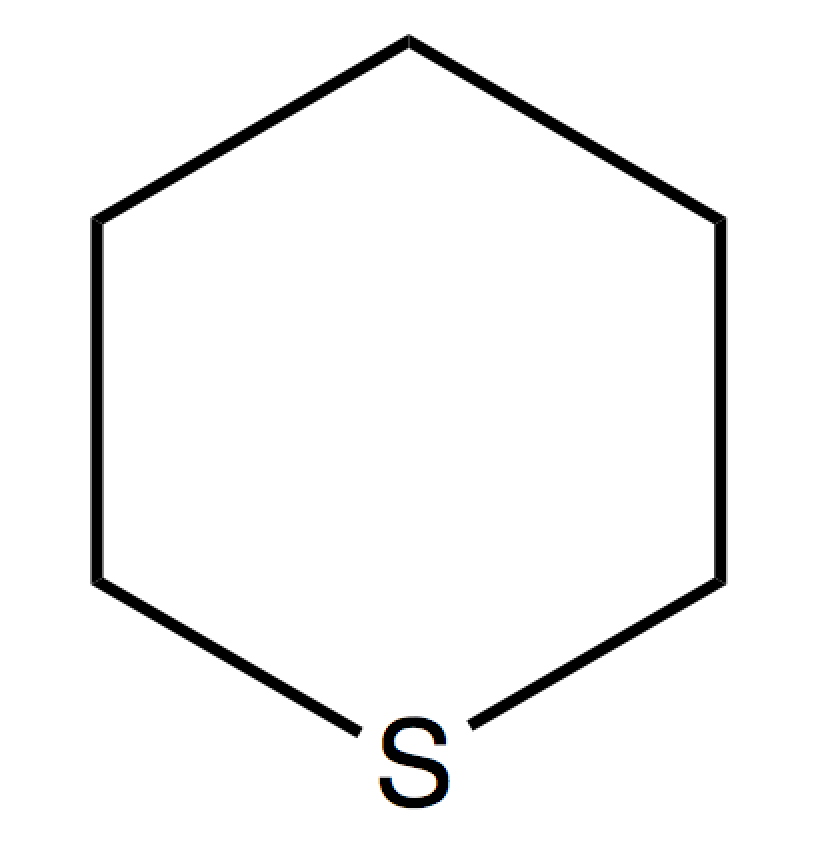
\includegraphics[scale=0.08]{image/sulfure-cycle} & Sulfures cycliques \\
			RSSR' & Disulfures \\
			 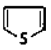
\includegraphics[scale=0.08]{image/thiophene} & Thiophène \\
			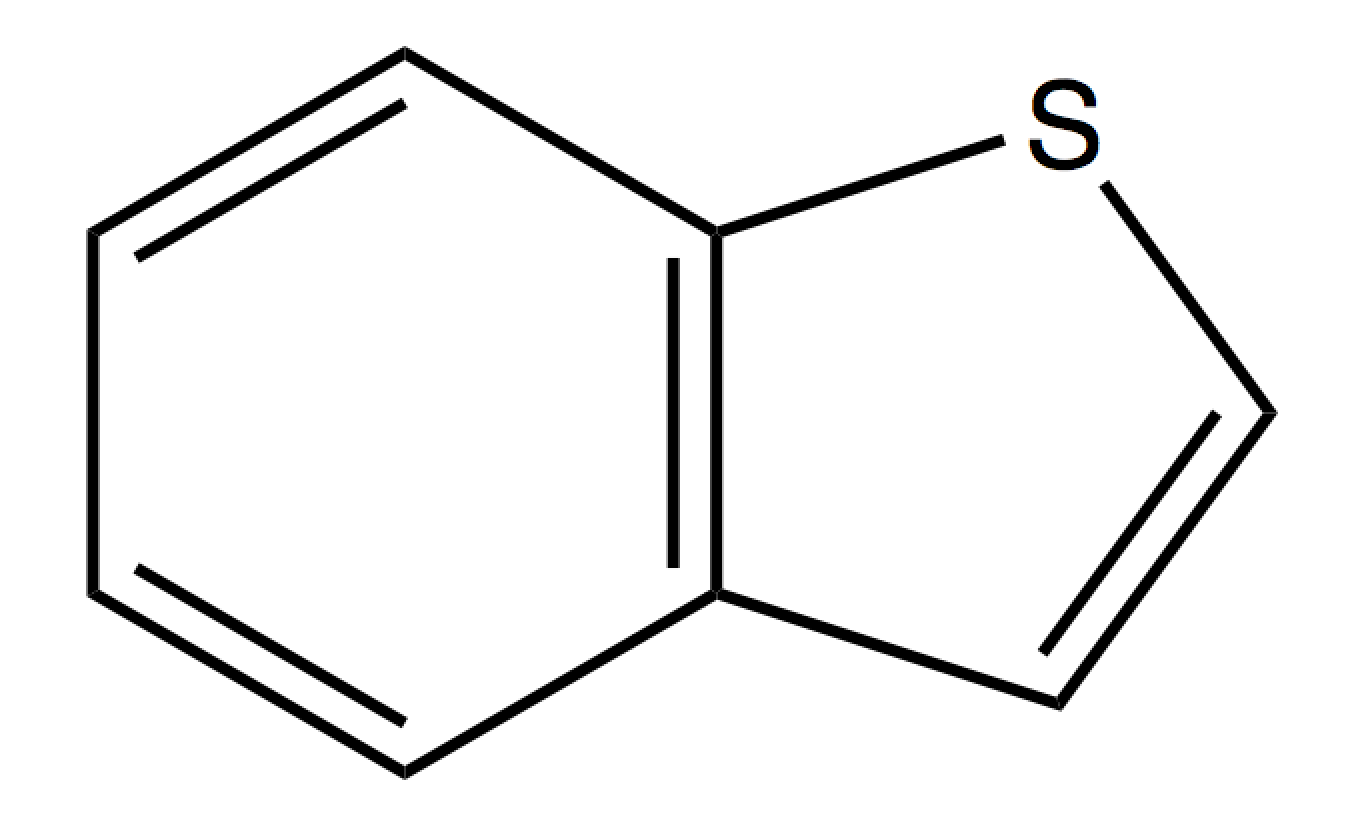
\includegraphics[scale=0.08]{image/benzothiophene} & Benzothiophène \\
			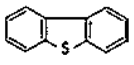
\includegraphics[scale=0.08]{image/dibenzothiophene} & Dibenzothiophène \\
			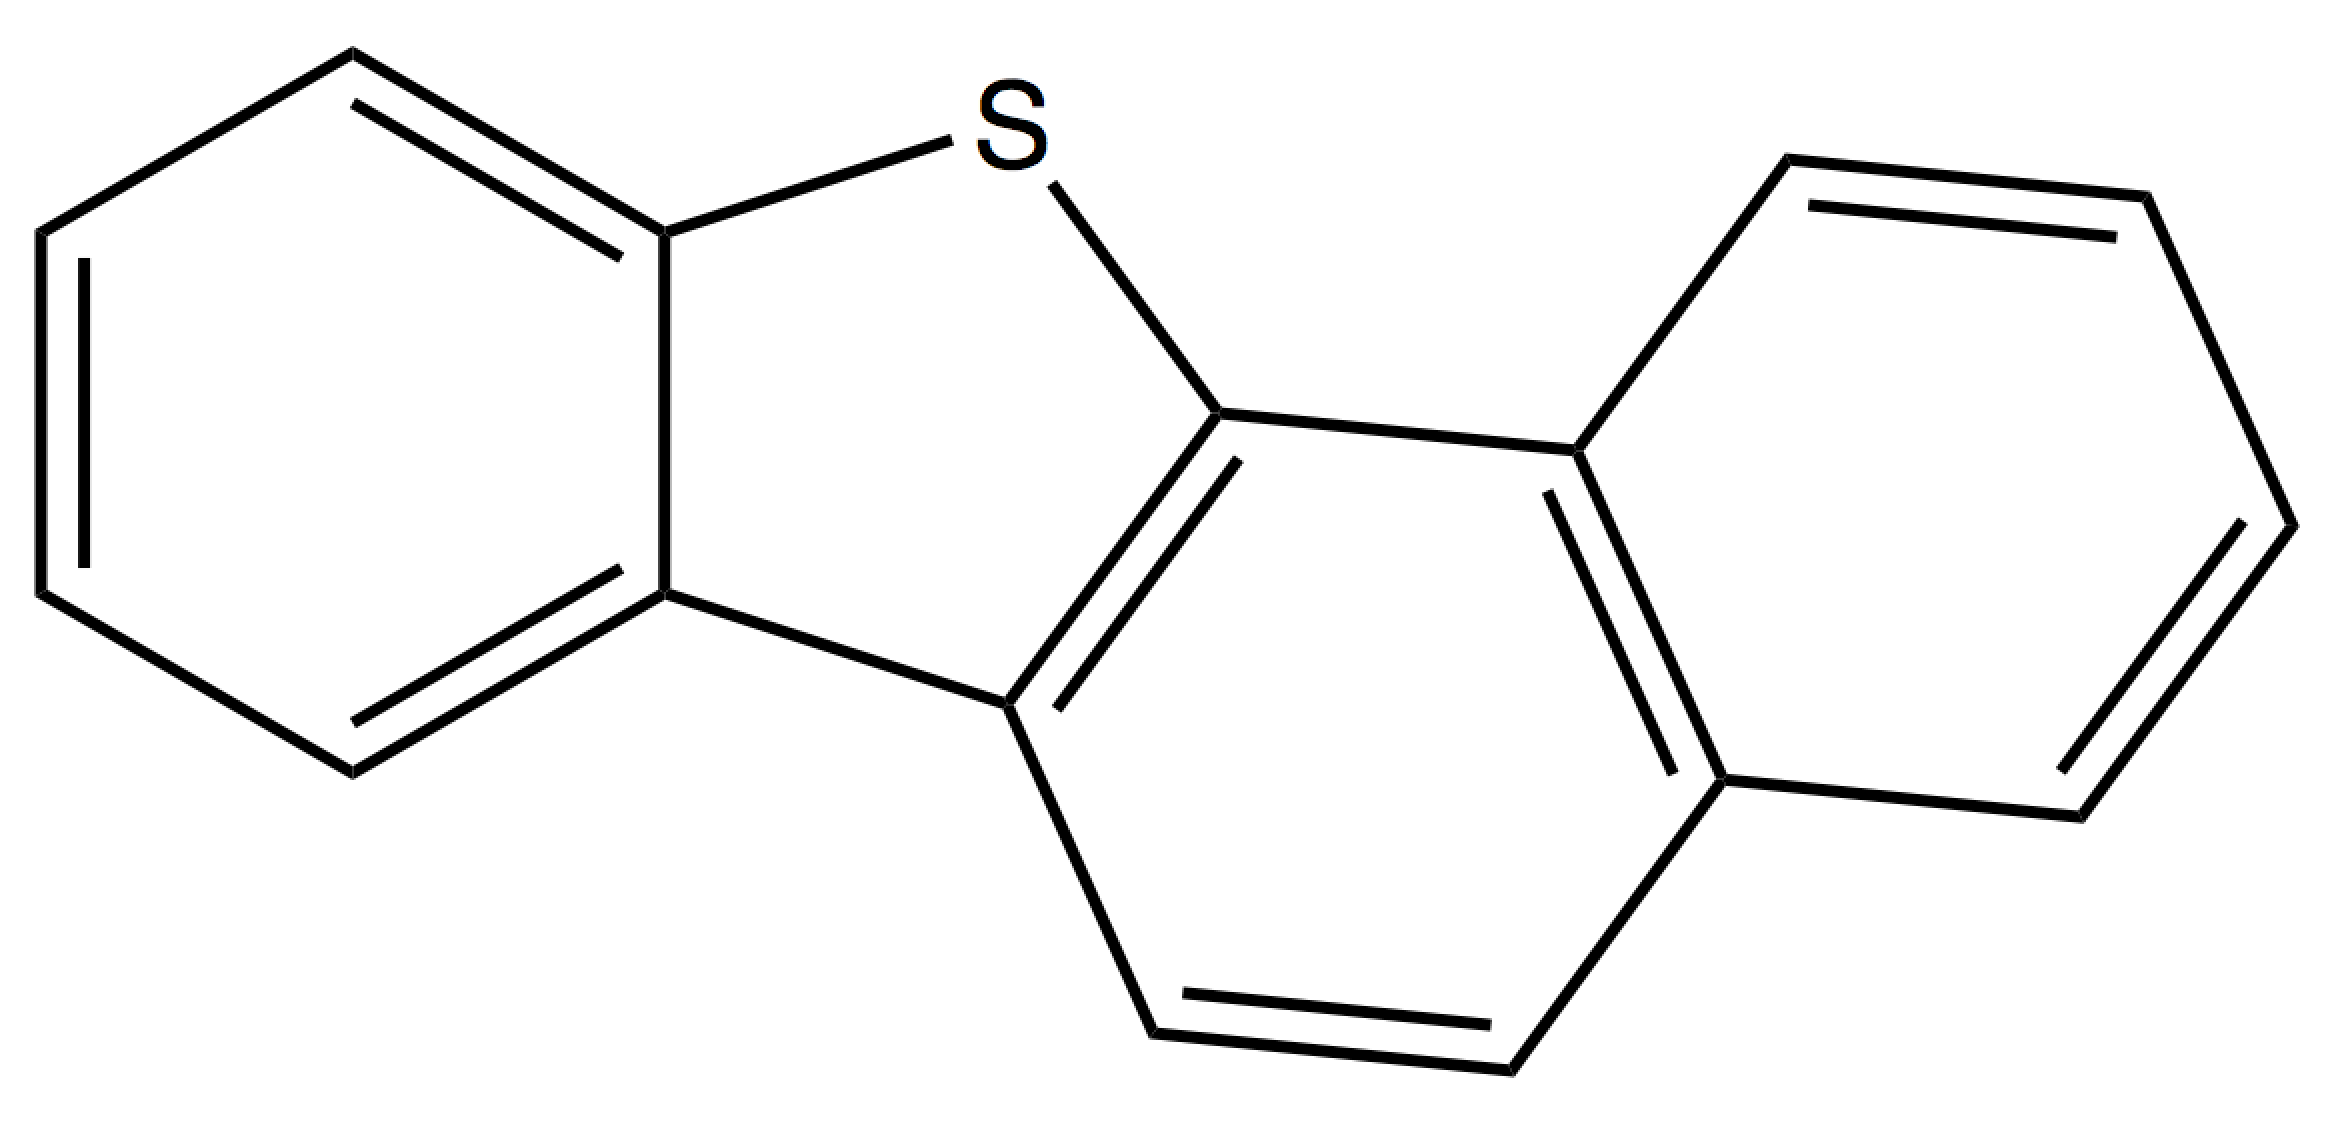
\includegraphics[scale=0.08]{image/naphto1} & Naphtobenzothiophènes \\
			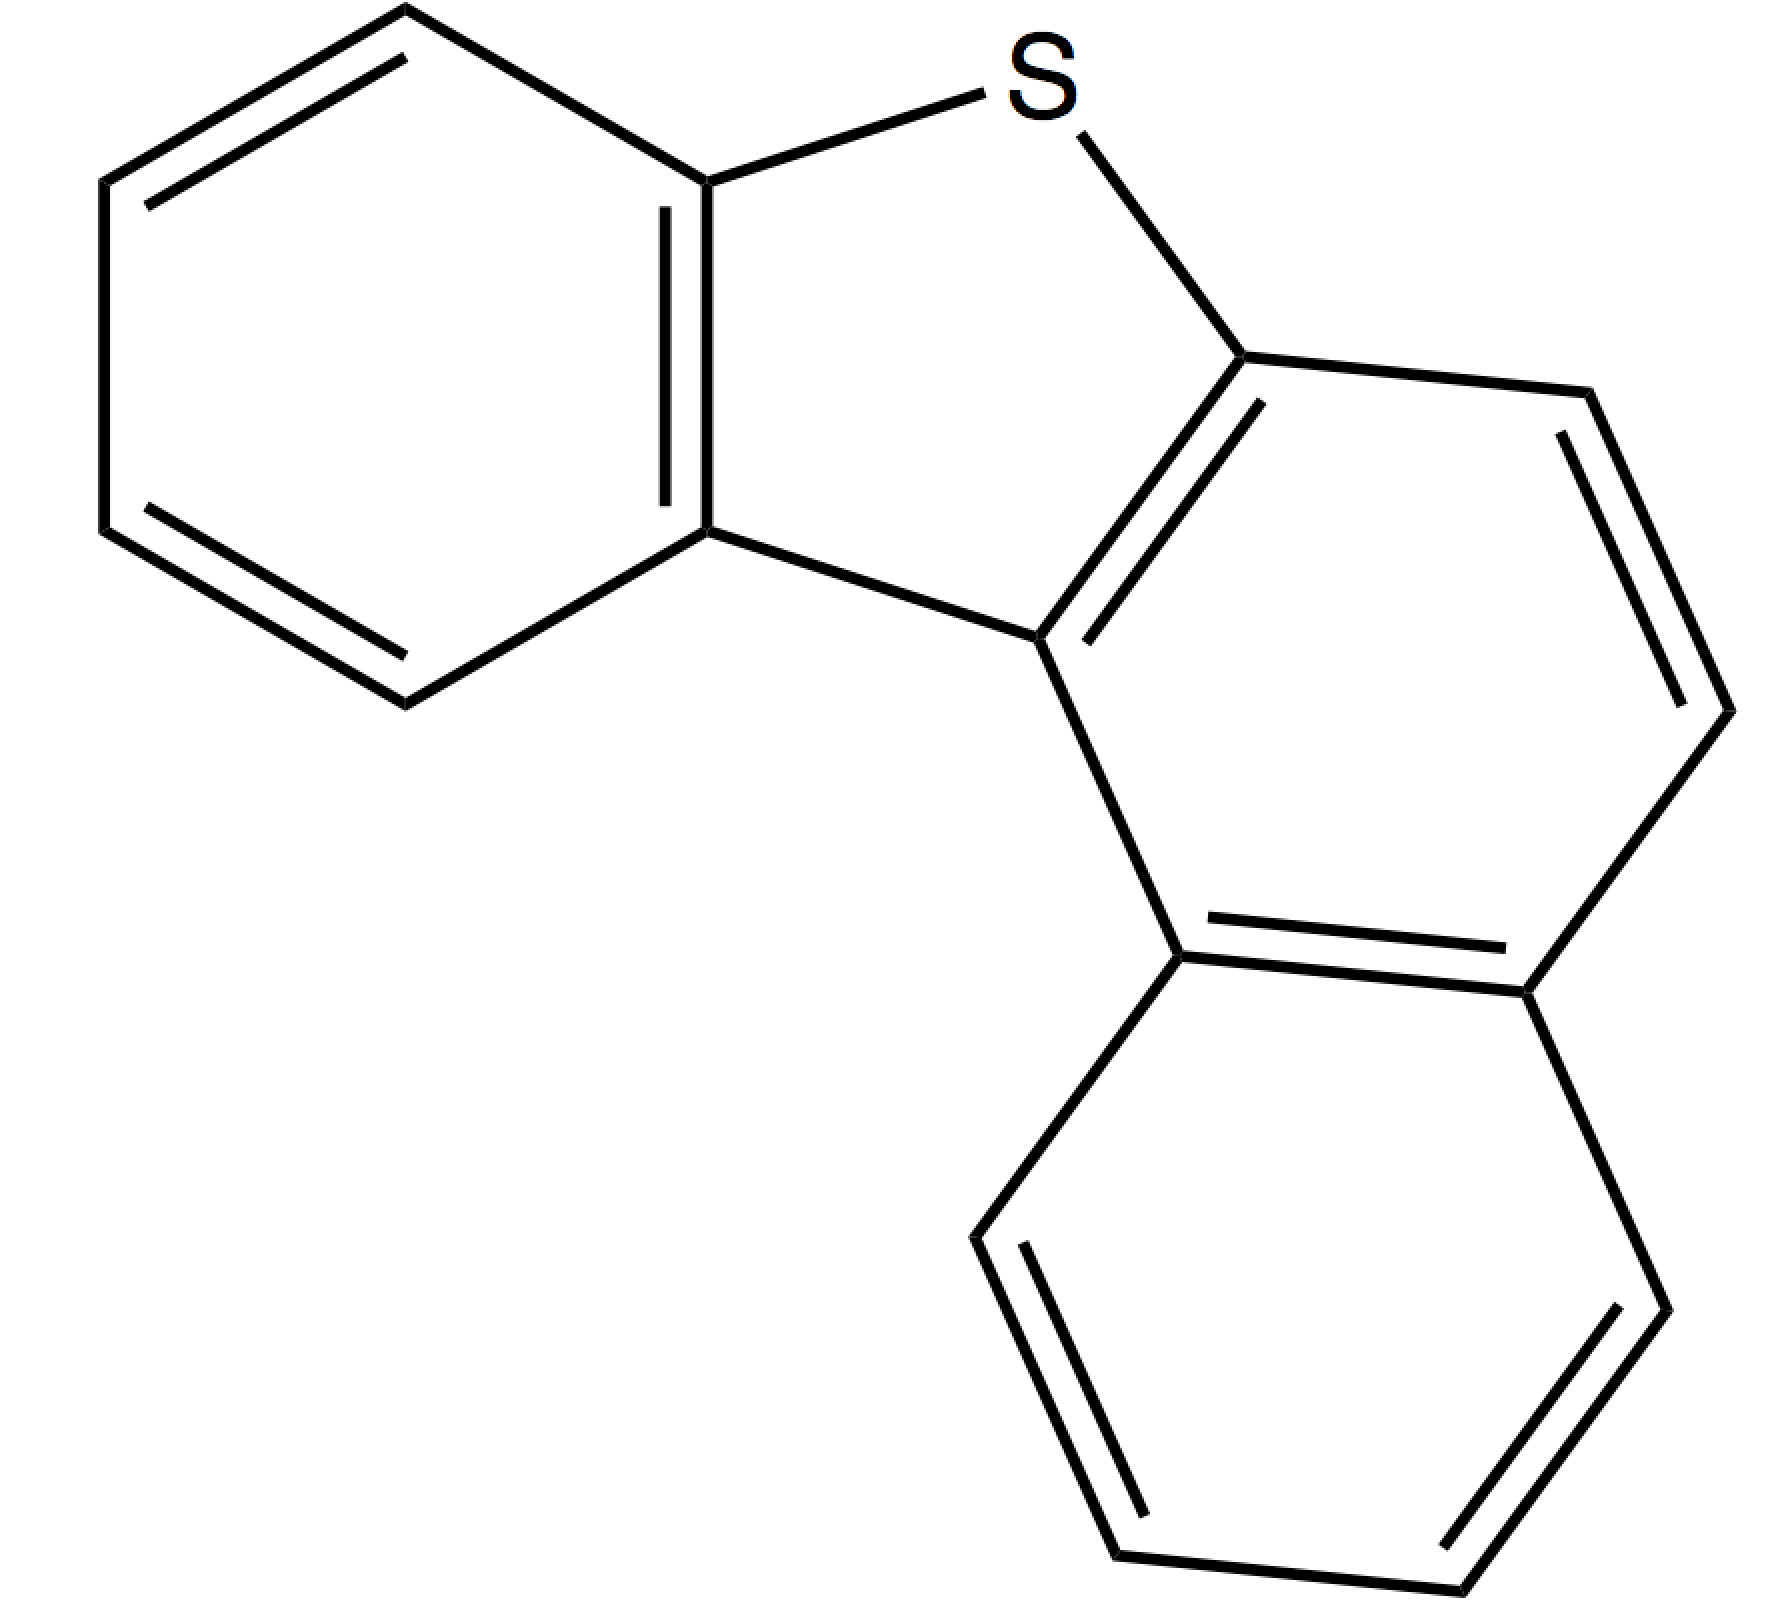
\includegraphics[scale=0.08]{image/naphto2} & \\
			\hline 
		\end{tabular}
	\end{center}
	\caption{Famille de composés soufrés caractérisés au sein du pétrole brut}
	\label{tab:soufre}
\end{table}


Thiols, sulfures, sulfoxydes et disulfides peuvent être classés plus précisément suivant leur nature cyclique ou acyclique, soit suivant l'organisation du squelette carboné (alkyle, aryle ou alkyl-aryle). Les dérivés thiophéniques, quant à eux, sont des structures polyaromatiques condensées autour d'un noyau thiophène (benzo, dibenzo, naphtobenzo-thiophènes, etc.). Au sein des fractions lourdes, la majorité des espèces soufrées sont des dérivés thiophéniques (cf. tableau \ref{tab:soufre-ex}), suivi par des dérivés sulfures (cycliques et acycliques). Enfin, des espèces de type sulfoxydes ont été mises en évidence, dans des proportions très variables, leur teneur variant entre 0.3\% et 10.3\% \cite{merdrignac2007physicochemical, speight2004petroleum}.

\begin{table}[h!]
	\begin{center}
		\begin{tabular}{rl}
			\hline
			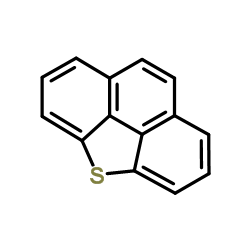
\includegraphics[scale=0.4]{image/phenanthro-thiophene} & Phénanthro-thiophènes \\
			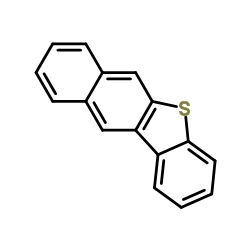
\includegraphics[scale=0.4]{image/benzo-naphto-thiophene} & Benzonaphto-thiophènes \\
			\hline 
		\end{tabular}
	\end{center}
	\caption{Exemples de dérivés thiophéniques courants identifiés au sein des fractions lourdes : phénanthro-thiophènes et benzonaphto-thiophènes}
	\label{tab:soufre-ex}
\end{table}


\paragraph{Azote}
En dépit des faibles proportions dans lesquelles il est présent, les dérivés de l'azote sont particulièrement étudiés, puisqu'à l'origine de la destruction des catalyseurs employés lors du craquage. Comme leurs analogues soufrés, les composés azotés se retrouvent en majeure partie au sein des fractions lourdes et des résidus de distillation du pétrole. \\
On distingue communément deux classes de composés azotés, à savoir les dérivés dits \og \textit{basiques} \fg, qui regroupent les homologues de la pyridine, et les dérivés dits \og \textit{neutres} \fg, qui rassemblent des systèmes de type pyrrole, indole et carbazole.  
En règle générale, environ un tiers des composés azotés sont des dérivés "basiques", la part restante revenant donc aux composés dits "neutres", bien que ces proportions puissent varier sensiblement en fonction des paramètres géochimiques de provenance du pétrole. \\
Comme indiqué dans le tableau \ref{tab:azote}, les structures "basiques" identifiées sont des analogues de la pyridine, tels que la quinoléine ou l'iso-quinoléine, comprenant entre deux et quatre cycles aromatiques condensés avec différents degrés d'alkylation ; des benzo- et dibenzoquinoléines, tétrahydroquinoléines, ainsi que des azapyrènes, ont par exemple pu être caractérisés, qui forment autant de systèmes à haut encombrement stérique. \\

\begin{table}[h!]
	\begin{center}
		\begin{tabular}{rl}
			\hline
			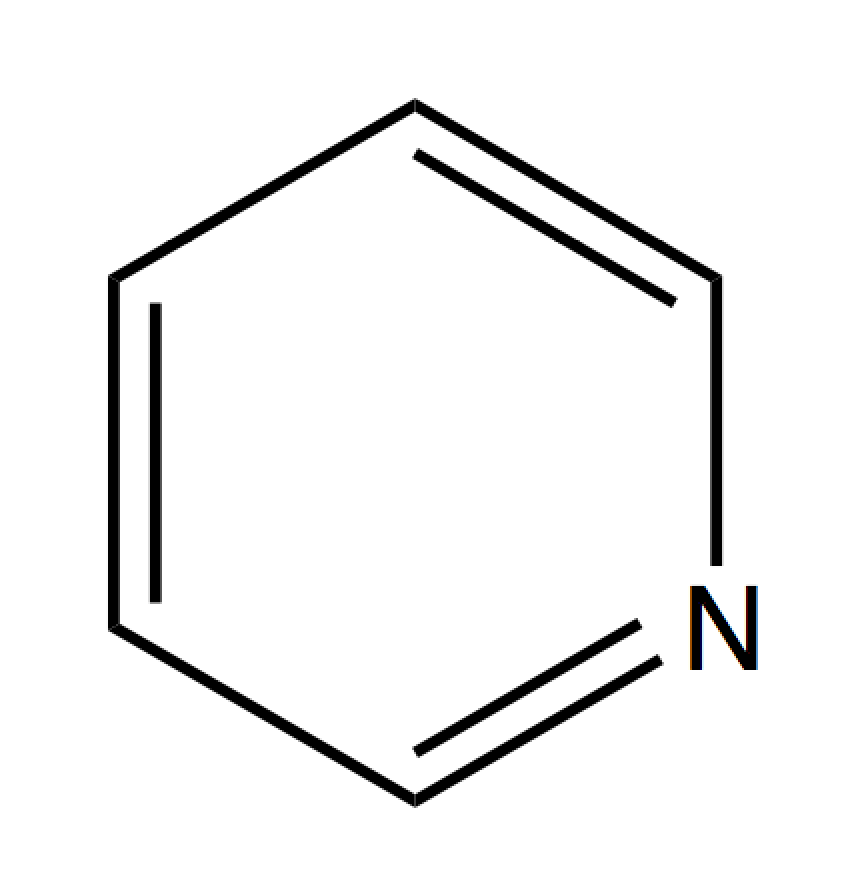
\includegraphics[scale=0.08]{image/pyridine} & Pyridine \\
			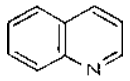
\includegraphics[scale=0.08]{image/quinoline} & Quinoline \\
			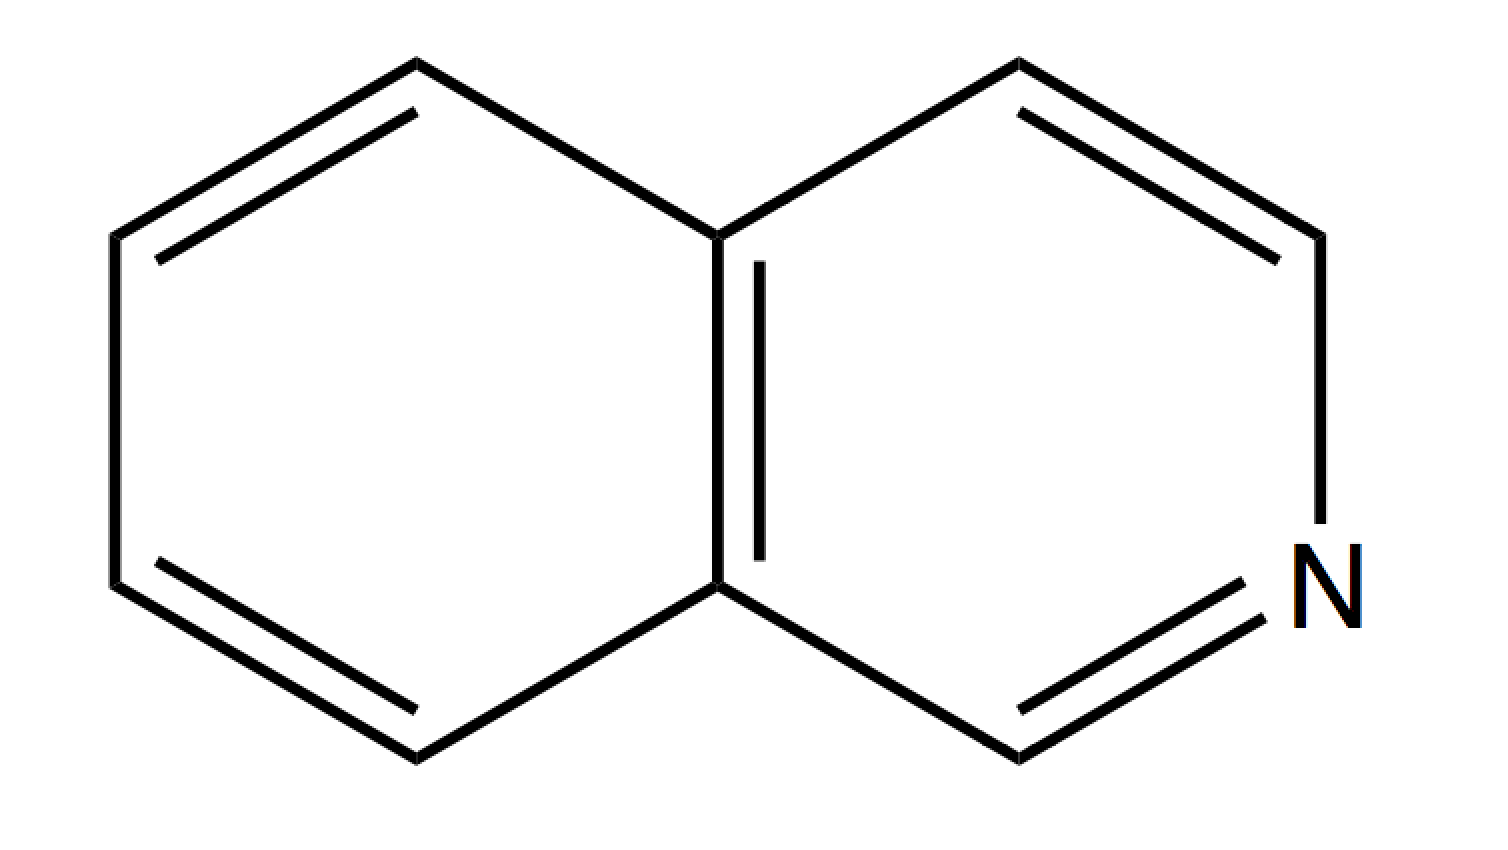
\includegraphics[scale=0.08]{image/isoquinoline} & Isoquinoline \\
			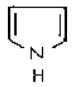
\includegraphics[scale=0.08]{image/pyrrole} & Pyrrole \\
			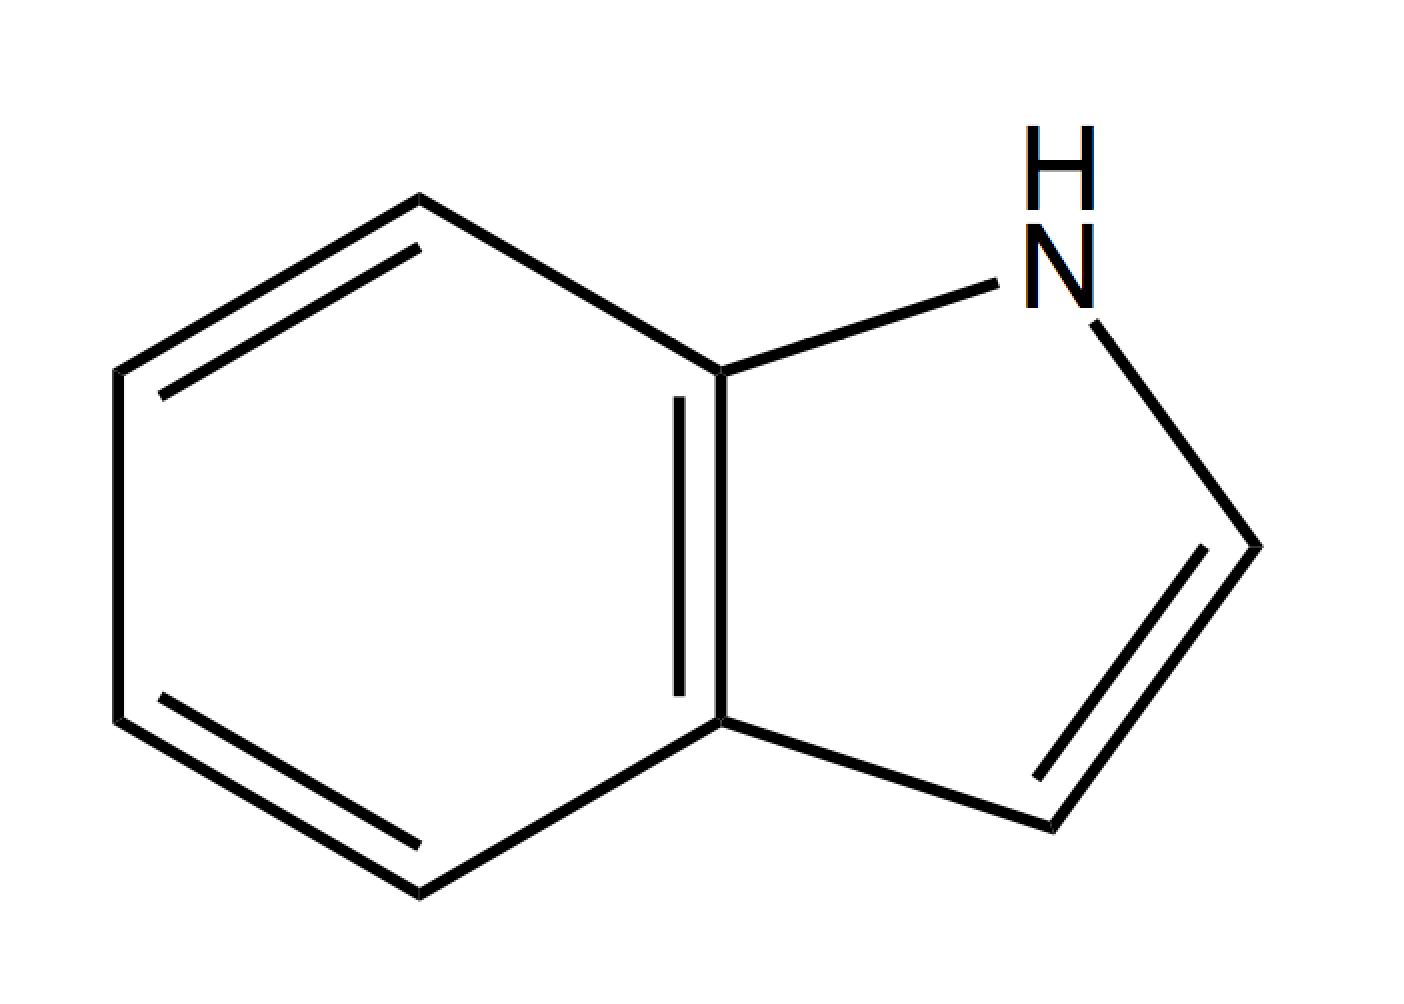
\includegraphics[scale=0.08]{image/indole} & Indole \\
			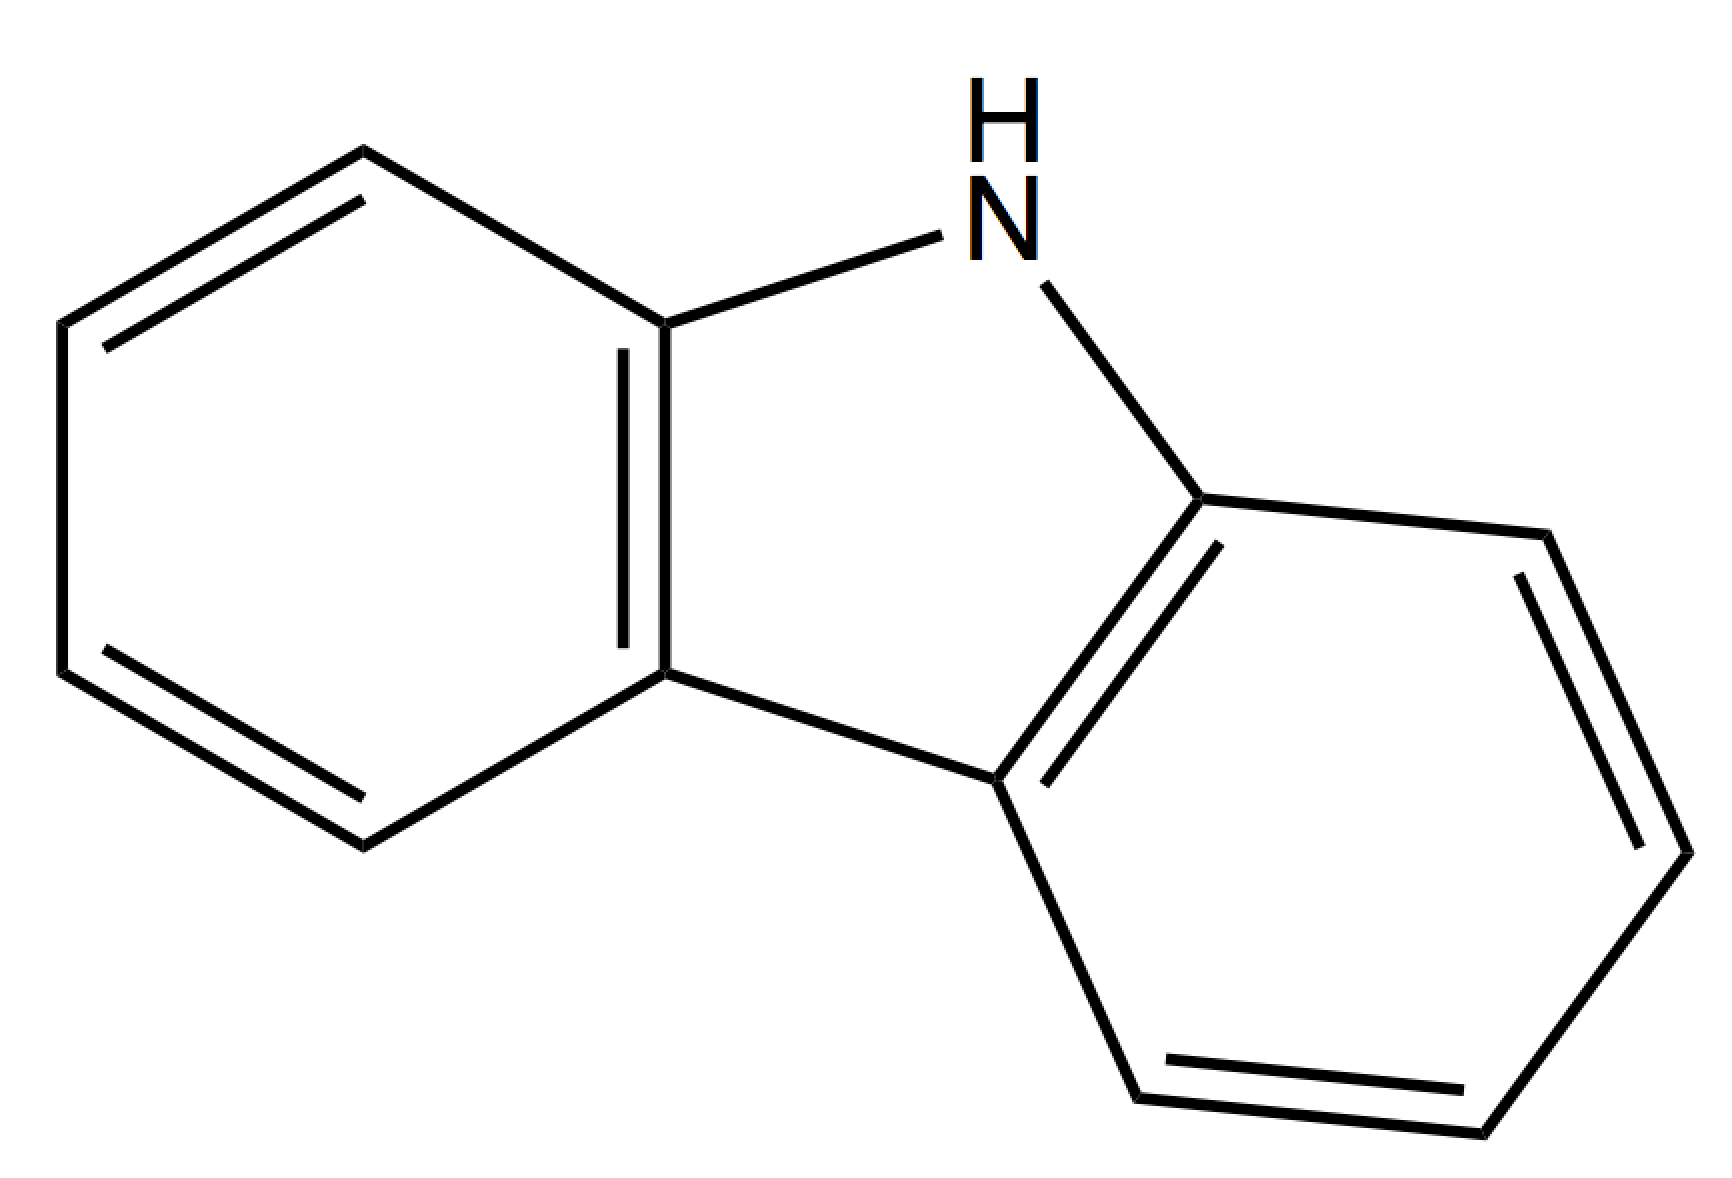
\includegraphics[scale=0.08]{image/carbazole} & Carbazole \\
			\hline 
		\end{tabular}
	\end{center}
	\caption{Famille de composés azotés caractérisés au sein du pétrole brut}
	\label{tab:azote}
\end{table}


Les structures "neutres", majoritaires, sont essentiellement représentées par les dérivés carbazolés (benzo-carbazoles, dibenzo-carbazole, etc.). C'est également au sein de cette classe de composés que l'on trouve les porphyrines qui, bien que présentes en proportions plus anecdotiques, possèdent une stabilité remarquable. La brique élémentaire de ces systèmes de grande taille est la molécule de pyrrole, et la plus simple des porphyrines est constituée par l'assemblage de quatre molécules de pyrrole [figure porphine !!!], reliées par des ponts méthylène =CH--. Le large système de résonance ainsi formé augmente considérablement la stabilité des structures ainsi formées. Par ailleurs, les porphyrines ont tendance à former des complexes métalliques avec les ions nickel et vanadium présents au sein du pétrole, par substitution des deux atomes d'hydrogène liés aux atomes d'azote de la structure porphyrinique. La proportion de ces structures au sein du pétrole dépend une nouvelle fois de l'origine géochimique de ce dernier, et un nombre croissant d'études s'intéresse à la part de métaux présents dans les huiles brutes. On estime aujourd'hui que ces complexes porphyrine-métaux représentent entre 0.6 et 3.3\% des fractions lourdes extraites\cite{merdrignac2007physicochemical, speight2004petroleum}.

\paragraph{Oxygène}
Au sein des fractions lourdes qui nous intéressent, la teneur en composés oxygénés varie entre 0.3 et 4.9\% \cite{speight2004petroleum}. Ces composés oxygénés figurent parmi les premières espèces caractérisées du pétrole. Les premiers travaux reportant la présence d'espèces acides au sein du pétrole remontent à 1874, et il faudra attendre quelques années de plus avant que celles-ci ne soient formellement identifiées comme étant des acides carboxyliques. Avec les dérivés du phénol, les acides carboxyliques représentent la majorité des espèces oxygénées constituant le pétrole, que l'on retrouve aussi bien dans les fractions lourdes qu'au sein de fractions plus légères. L'ensemble des études réalisées sur le sujet tend à établir que la structure de ces acides carboxyliques correspond à la structure de l'hydrocarbure prévalent. En d'autres termes, la structure de l'acide dépend du nombre d'atomes de carbone que compte le squelette carboné de l'hydrocarbure. Ainsi, lorsque l'acide comporte moins de huit atomes de carbone, ce qui correspond à un hydrocarbure de type paraffinique comme évoqué ci-avant, sa structure sera de type aliphatique. Suivant cette logique, des acides comportant un cycle commencent à apparaître à partir de six atomes de carbone et ces structures monocycliques prédominent jusqu'à quatorze atomes de carbone environ. \\
Une caractérisation plus fine des groupements carboxyles en présence révèle également la coexistence d'esters, de cétones, d'amides, d'anhydrides, d'éthers et de sulfoxydes. Néanmoins, à la différence des acides carboxyliques, plus aisés à caractériser puisque présent tant dans les fractions lourdes que dans les fractions légères, ces composés oxygénés se retrouvent majoritairement dans les fractions lourdes et leurs structures sont de fait plus complexes à identifier. Il est par ailleurs à noter que certains de ces composés sont supposés provenir de réactions entre les résidus de distillation et l'oxygène soufflé, qui intervient notamment dans les procédés de production de l'asphalte. De fait, il est difficile de conclure quant au fait que toutes ces espèces sont ou non des constituants du pétrole brut. 


\subsubsection{Débat autour du poids moléculaire des asphaltènes}

Un rapide passage en revue de la bibliographie des asphaltènes révèle tout le débat autour de leur poids moléculaire. En effet, la distribution, en termes de poids moléculaire, varie entre 400 et 1500 Da pour les fractions de faible poids moléculaire, et peut atteindre $10^{6}$ Da pour les fractions de haut poids moléculaire \cite{mullins2008contrasting}. Le phénomène d'agrégation des asphaltènes est une des raisons avancées pour justifier qu'à l'heure actuelle aucune méthode n'ait permis de déterminer avec précision le véritable poids moléculaire de ces espèces. De nombreux procédés ont été employés pour tenter de résoudre ce problème, mais ceux-ci conduisent à des résultats ambigüs, qu'il serait hasardeux de généraliser. À titre d'exemple, des mesures par osméométrie à tension de vapeur font apparaître des résultats fortement dépendants du type de solvant employé ; en présence d'un solvant apolaire tel que le toluène, les résultats apparaissent surestimés, au contraire de l'utilisation d'un solvant polaire tel que la pyridine ou le nitrobenzène. 
%S'agissant d'autres méthodes d'analyse, Groenzin et Mullins\cite{groenzin2000molecular} parviennent, par spectroscopie de fluorescence résolue en temps, à un poids moléculaire moyen de 750 Da environ, pour une distribution de 500 à 1000 Da, là où Pinkston et col.\cite{pinkston2009analysis} rapportent une distribution de 350 à 1050 Da pour une étude par spectrométrie de masse de résonance cyclotronique ionique à transformée de Fourier (FT-ICR). Ces derniers supposent l'existence de fragments de plus bas poids moléculaires, non détectés même à haute énergie électronique du fait de la stabilisation des intermédiaire obtenus par les chaînes alkyles des asphaltènes. 

%Merdrignac et col.\cite{merdrignac2006evolution} rapportent l'évolution du poids moléculaire des asphaltènes et comparer les changements causés par le procédé d'hydroconvertion. 


%\subsubsection{Une inconnue : la structure des asphaltènes}

\section{État des lieux des connaissances sur les systèmes asphalténiques}

La description de la structure des asphaltènes repose à l'heure actuelle sur deux modèles construits sur la base des résultats de diverses caractérisations expérimentales.  
Le premier modèle, baptisé modèle \og continental \fg, représente les asphaltènes comme de larges cœurs constitués de quatre à dix cycles aromatiques condensés, ramifiés par des chaînes alkyles courtes \cite{groenzin2000molecular} (cf. figure \ref{figZ1}). Ce modèle a été proposé par Zhao \textit{et al.} \cite{zhao2001molecular} après caractérisation des asphaltènes obtenus par fractionnement avec du pentane supercritique, puis remployé par Rogel et Carbognani \cite{rogel2003density} dans leur travail sur des asphaltènes stables et instables extraits de pétrole provenant du Vénézuela. 
Ce type de représentations est corrélé par des analyses en spectroscopie RMN, diffraction des rayons X et spectroscopie de fluorescence résolue en temps (TRDF). 



\begin{figure}[h!]
	\centering
	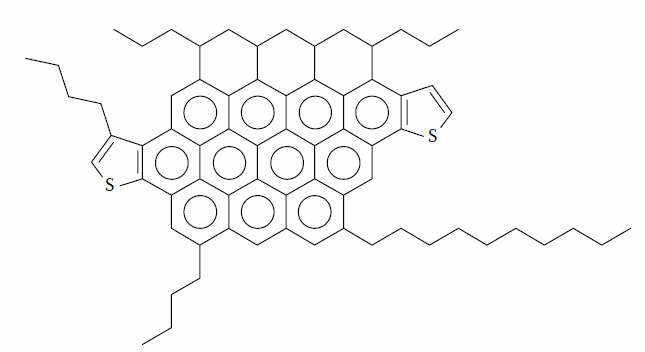
\includegraphics[height=5cm]{image/Zhao}
	\caption[Structure moyenne du modèle continental des asphaltènes]{Structure moyenne du modèle continental des asphaltènes (Zhao et col. \cite{zhao2001molecular})}
	\label{figZ1}
\end{figure}


Le modèle "archipel" présente quant à lui ces systèmes comme un ensemble de régions à caractère aromatique, constituées de deux à trois cycles condensés, reliées par des chaînes carbonées. Ce modèle s'appuie sur des analyses par pyrolyse, oxydation, dégradation thermique et dispersion angulaire neutronique, telles que rapportées par Gawrys \textit{et al.} \cite{gawrys2003role}. Sheremata \textit{et al.}\cite{sheremata2004quantitative} ont notamment employé ce modèle pour la description des asphaltènes, comme le présente la figure reproduite ci-après (figure \ref{fig2}). 

\begin{figure}[h!]
	\centering
	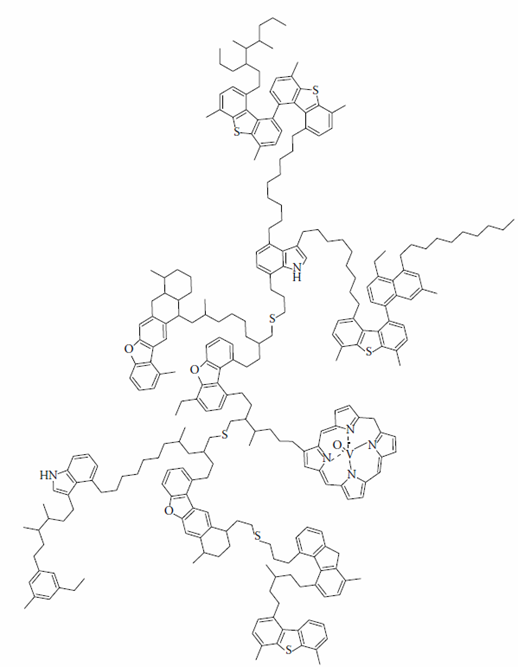
\includegraphics[height=8cm]{image/Sher}
	\caption[Molecule d'asphaltènes type archipel]{Représentation d'asphaltènes à l'aide du modèle archipel, proposé par Sheremata \textit{et al.}\cite{sheremata2004quantitative}}
	\label{fig2}
\end{figure}

Ces deux modèles, basés sur des structures moléculaires bien distinctes, conduisent néanmoins à des propriétés physico-chimiques différentes. La description des agrégats d'asphaltènes ainsi que leur solubilité dans le pétrole brut seront nettement impactées par l'emploi de l'une ou l'autre de ces représentations. Du fait de la planéité induite par la présence d'un grand nombre de cycles aromatiques condensés, la représentation d'un agrégat d'asphaltènes dans le cadre du modèle continental conduit à un empilement de plans. À l'inverse, les chaînes alkyles du modèle archipel confèrent une toute autre géométrie à ces systèmes : les asphaltènes peuvent se courber par le biais d'interactions intermoléculaires pour former des macro-agrégats globulaires susceptibles de piéger les molécules de solvant. \bigskip

Le paragraphe qui suit se veut résumer les nombreuses analyses expérimentales menées sur ces systèmes, analyses qui ont dans un premier temps permis l'émergence des deux modèles que nous venons d'évoquer, avant de travailler à les confirmer ou les infirmer. 

\subsection{Revue des données expérimentales}

\subsubsection{Analyses par spectroscopie RMN}

La spectroscopie de résonance magnétique nucléaire est couramment employée pour l'analyse structurale et la caractérisation de matériaux et de substances organiques. 
%Elle est fondée sur les propriétés magnétiques de certains noyaux atomiques.Les noyaux les plus étudiés, dans le cadre de la chimie organique sont l'hydrogène $^{1}H$ et le carbone $^{13}C$. 
Cette technique représente donc une méthode d'analyse de choix pour l'étude des asphaltènes et a, à ce titre, permis d'acquérir les premiers résultats visant à résoudre leur composition chimique. Dès 1982, les travaux de Murphy \textit{et al.} \cite{murphy1982determination} révèlent que la structure primaire des asphaltènes se compose de multiples cycles aromatiques condensés (l'indice de condensation relevé sur ces systèmes étant de 3 au moins) ainsi que d'une grande variété de chaînes aliphatiques, longues et ramifiées. Par la suite, les travaux de Yen \textit{et al.} en RMN $^{1}H$ ont donné une première idée de la proportion d'hydrocarbures saturés en regard de la fraction d'hydrocarbures aromatiques au sein de molécules d'asphaltènes  \cite{yen1984study}. Enfin, plus récemment, Durand \textit{et al.} ont employé les résultats de leurs analyses par RMN $^{13}C$ pour évaluer les indices de substitution et de condensation d'échantillons d'asphaltènes de différentes origines \cite{durand2010effect}. Leur étude tend à démontrer qu'au sein d'agrégats d'asphaltènes cohabitent les deux modèles structuraux évoqués ci-avant, à savoir le modèle continental et le modèle archipel. 


\subsubsection{Analyses par diffraction des rayons X}  

Une étude du caractère aromatique et des paramètres cristallins des asphaltènes, des résines et des gilsonites issus du pétrole a été présentée par Yen \textit{et al.} sur la base d'analyses en diffraction des rayons X \cite{yen1961investigation}. Leurs résultats, confortés par les travaux réalisés par Shirokoff \textit{et al.} sur quatre échantillons d'asphaltènes issus d'huiles brutes provenant d'Arabie Saoudite \cite{shirokoff1997characterization}, représentent les asphaltènes comme des feuillets de cycles aromatiques condensés portant des ramifications de natures naphténiques et aromatiques.
Toutefois, Altget et Boduszynky rappellent judicieusement dans leur étude \cite{altgeltcomposition} qu'il convient de prendre avec précaution les résultats provenant d'analyses de diffraction, lorsque les données géométriques fournies par l'analyse servent de base pour construire un modèle structural du système étudié. Leurs travaux semblent en outre indiquer que la détermination du caractère aromatique des asphaltènes est, par ce biais, inappropriée sinon arbitraire. 



\subsubsection{Analyses par spectroscopie de fluorescence résolue en temps} 

Cette méthode d'analyse a été employée à plusieurs reprises pour tenter d'élucider plus précisément la taille et la structure de molécules d'asphaltènes faiblement agrégées.  
Les premiers travaux en ce sens, réalisés par Groenzin et Mullins  \cite{groenzin1999asphaltene}, tendent à montrer que les molécules d'asphaltènes ne seraient constituées que d'un seul groupe chromophore. En effet, le faible poids moléculaire obtenu pour ces systèmes, comme la coloration des molécules, sont autant d'éléments recueillis incompatibles avec la représentation des asphaltènes sous forme de larges structures pseudo-polymériques constitués de deux ou trois cycles aromatiques reliés entre eux par de longues chaînes aliphatiques. En définitive, ces premières analyses par spectrométrie de fluorescence semblent conforter la représentation des asphaltènes par le modèle continental. \\
Par la suite, Souza \textit{et al.} ont rapporté l'agrégation persistante des asphaltènes à la faible concentration de 0.8 g/L, soit sous le seuil de concentration critique de nanoagrégation \cite{souza2009study}. Leurs travaux corroborent par ailleurs les résultats de Groenzin \textit{et al.}\cite{groenzin1999asphaltene} quant à la structure de type \og continental \fg{} des molécules d'asphaltènes, en cela qu'ils concluent à une structure primaire constituée d'un anneau polyaromatique de quatre cycles ou plus. 




\subsubsection{Analyses par spectroscopie infrarouge}

La caractérisation d'un système chimique en termes de composition passe nécessairement par des analyses en spectroscopie infrarouge, laquelle permet l'identification des groupements fonctionnels. Toutefois, dans le cadre de l'étude des fractions lourdes du pétrole, la diversité chimique et la taille des espèces présentes rendent complexe l'utilisation de la spectroscopie IR. C'est ce que soulignent Yuan \textit{et al.}, qui relèvent l'existence d'un faible nombre d'analyses employant l'infrarouge moyen pour la caractérisation physique et chimique des huiles lourdes \cite{hongfu2006determination}. 
Parmi les travaux notables, l'étude couplée en spectroscopies IR et UV-sisible menée par El-Bassoussi \textit{et al.}\cite{el2010characterization} sur deux échantillons d'asphaltènes provenant d'Egypte a permis de classifier les espèces présentes en mono, di et polyaromatiques. En accord avec les deux modèles de représentation des asphaltènes, les espèces prédominantes sont les espèces di ou polyaromatiques. En 2007, Rodrigues Coelho \textit{et al.} \cite{coelho2007characterization} démontrent l'existence d'une corrélation linéaire entre les intensités des bandes infrarouges symétriques et antisymétriques associées aux atomes d'hydrogène aromatiques de type arènes méthyl-substitués dans les régions 2900-3100 $cm^{-1}$ et 700-900 $cm^{-1}$. Enfin, Laxalde \textit{et al.} \cite{laxalde2014combining} rapportent une interprétation, toutefois ajustée sur les structures modèles des asphaltènes, en repérant les vibrations de stretching des liaisons C-H (hors du plan) et C=C.

\bigskip

\subsubsection{Conclusion : les asphaltènes, une coexistence de structures moléculaires ?}

La compilation de l'ensemble de ces résultats expérimentaux tend à suggérer que les deux modèles structuraux des asphaltènes peuvent coexister au sein des fractions lourdes. Cette idée est appuyée par les résultats d'Acevedo \textit{et al.} \cite{acevedo2004structural, gutierrez2001fractionation} qui ont montré que les asphaltènes pouvaient se diviser en deux fractions : une fraction insoluble dans le toluène, baptisée A1, qui serait rigide et plane, conformément au modèle continental, et une fraction soluble dans le toluène grace à de nombreuses interactions intermoléculaires, baptisée A2 et qui correspondrait au modèle archipel. Sur la base de ces éléments, Acevedo et son équipe ont mis en place une nouvelle représentation des agrégats d'asphaltènes. Le système colloïdal consisterait en une fraction d'asphaltènes A1, entourés par une couche d'asphaltènes A2, ces derniers aidant à la solubilisation de l'ensemble. \\
En définitive, une revue bibliographique des analyses expérimentales menées à ce jour sur les asphaltènes montre qu'aucun modèle structural définitif valide n'a encore émergé pour ce type de systèmes. De nombreux travaux cherchent encore à clarifier l'architecture moléculaire des asphaltènes, à deux échelles distinctes. En premier lieu, l'étude de la microstructure correspond à des systèmes de poids moléculaires variant entre 500 et 10 000 Da, soit à des nano-agrégats d'asphaltènes. En second lieu, les travaux sur la macrostructure de ces entités correspondent à l'étude d'assemblages de ces nano-agrégats d'asphaltènes et sont intimement liés au milieu. 



\subsection{La modélisation, outil indispensable dans l'élucidation des structures asphalténiques}

\subsubsection{Des nombreux intérêts de la modélisation des asphaltènes}

La chimie computationnelle a révolutionné notre façon d'appréhender la structure et la réactivité des molécules, de sorte que la simulation est désormais une des clés de voûte de l'avancée scientifique. \\
Comme nous l'avons souligné dans le paragraphe précédent, la nature et la complexité des asphaltènes rendent impossible leur caractérisation exhaustive par le seul biais de données expérimentales. Dans ce cadre, l'intérêt des simulations est incontestable et nombreux sont les travaux qui se sont déjà penchés sur la configuration moléculaire, les interactions intermoléculaires, la stabilité ou les phénomènes d'agrégation de ces systèmes.  
Concernant ce dernier point, la modélisation moléculaire a permis de justifier que l'agrégation des asphaltènes représentait la conformation la plus stable, sur la base d'une double approche structurale et thermodynamique révélant les interactions avec les résines, présentes au sein des fractions lourdes, et les solvants \cite{murgich1996molecular}. Selon ces travaux, l'interaction responsable de la formation comme de la stabilité des micelles formés d'asphaltènes et de résines serait la force d'attraction qui s'exerce entre les plans aromatiques. 
D'autres études théoriques se fondent sur les modèles structuraux proposés pour les asphaltènes. Les orbitales moléculaires de dimères d'asphaltènes, envisagés successivement par les modèles continental et archipel, ont été étudiés dans une approche semi-empirique ZINDO après optimisation des structures en DFT (théorie de la fonctionnelle de la densité). Du point de vue de la stabilité, la configuration continentale, représentée dans les simulations par des dimères empilés pour symboliser les plans d'asphaltènes propres à ce modèle, s'avère globalement plus stable que la configuration archipel \cite{alvarez2013island}. 


\subsubsection{Construction de la structure moléculaire des asphaltènes}

La construction d'un modèle moléculaire utilisable en simulation se fait sur la base des données expérimentales recueillies, suivant deux méthodes principales. \\
La première méthode repose sur une corrélation des résultats empiriques utilisés pour déduire des informations structurales. Dans le cas des asphaltènes, l'existence de nombreux cycles aromatiques et l'ensemble des données obtenues concernant la longueur des chaînes aliphatiques ont permis à Takanohashi \textit{et al.} d'étudier trois structures distinctes d'asphaltènes générées par la méthode de Sato par le biais de simulation en dynamique moléculaire \cite{takanohashi2004structural}. \\
La seconde méthode consiste à identifier des caractéristiques structurales propres au système, ainsi que sa composition moléculaire, en suivant un processus stochastique. Le modèle structural se construit alors par addition des données expérimentales et/ou par recoupement de ces résultats avec une base de données existantes. Cette méthode a été poursuivie aussi bien par Elyashberg \textit{et al.} \cite{elyashberg2008computer}, qui ont développé un algorithme permettant la construction d'une structure sur la base de données RMN, que par Todeschini \textit{et al.} \cite{todeschini1995weighted} qui ont quant à eux employé des propriétés physiques telles que l'hydrophobie, le point de fusion et le point d'ébullition. 
La construction d'un modèle moléculaire des asphaltènes peut en dernier lieu se faire initialement de façon plus intuitive, les informations expérimentales servant ensuite à optimiser le modèle de départ \cite{faulon1996stochastic}, \cite{al2012systematic}, \cite{de2012monte}. 





\newgeometry{textwidth=16cm}
\chapter{Partie vibrationnelle}
\minitoc
\restoregeometry

\newpage


% % % % % % % % % % % % % % % % % % % % % % % % % % % % % % % % % % % % % % % % % % % % % % % % % % % % % % % % 
% % % % % % % % % % % % % % % % % % % % % % % % % % % % % % % % % % % % % % % % % % % % % % % % % % % % % % % % 
% % % % % % % % % % % % % % % % % % % % % % % % % % % % % % % % % % % % % % % % % % % % % % % % % % % % % % % % 

\section*{Introduction}
\markright{INTRODUCTION}{}

La littérature consacrée aux applications des spectrométries vibrationnelles dans le domaine de la caractérisation des constituants présents dans les pétroles est relativement peu abondante, et ce bien que la spectrométrie infrarouge soit devenue une technique d'analyse de \og routine \fg{} dans de très nombreux laboratoires, académiques comme industriels. La raison de cette faible abondance réside essentiellement dans la complexité des mélanges qui constituent un pétrole, un asphaltène, etc.. Pourtant, les champs d'application de cette technique se sont considérablement développés depuis l'apparition sur le marché de spectrophotomètres à transformée de \textsc{Fourier}.
Après avoir vu sa position privilégiée menacée par d'autres méthodes, telles que la spectroscopie RMN\footnote{\og Nuclear Magnetic Resonance Spectroscopy \fg{}.} ou la spectrométrie de masse, la spectrométrie infrarouge à transformée de \textsc{Fourier} (IRTF) a connu de nouvelles avancées technologiques, parmi lesquelles la spectrométrie photoacoustique que nous avons employée dans ce travail, qui lui confèrent à l'heure actuelle une précision d'analyse permettant d'atteindre des informations détaillées sur :

\begin{itemize}
	\item la structure chimique de molécules, de macromolécules : identification de l'unité de base, des ramifications ; analyses des extrémités de chaînes ; identification des défauts, d'éventuelles impuretés\dots{}
	\item les interactions intra et inter-moléculaires, la conformation des chaînes, l'orientation des molécules et des macromolécules, les auto-associations éventuelles, \dots{}
\end{itemize}

Cette partie a pour but essentiel de définir le vocabulaire et les notions fondamentales que nous emploierons par la suite, le développement détaillé du traitement classique de la vibration se trouvant dans de nombreux ouvrages et repris dans de nombreuses thèses. Parallèlement à ces développements expérimentaux, la modélisation en spectroscopie vibrationnelle a connu ces dernières décennies de très grandes mutations. Ce chapitre vise également à rappeler les fondements essentiels de la résolution de l'équation vibrationnelle de Schr\"{o}dinger, qui sous-tendent les principales méthodes -- que nous développerons -- actuellement disponibles pour tenter de répondre aux problématiques posées par les expérimentateurs. 


Le domaine de la pétrochimie qui nous intéresse dans ce travail, et précisément la thématique visant à l'élucidation de la composition de ces mélanges complexes, composés de milliers de molécules différentes non encore identifiées, est un domaine au champ d'investigation large et pour lequel les attentes sont grandes en termes de caractérisation comme de compréhension des processus d’interaction et d’agrégation de ces molécules. Dans ce domaine encore, la spectrométrie IRTF est certainement un des outils les plus efficaces pour élucider les mécanismes impliqués, mais les données résultantes sont complexes et de fait difficilement interprétables et justifiables sans un support théorique adapté.

L'Équipe de Chimie Physique (ECP) de l'IPREM est depuis très longtemps spécialisée dans les développements méthodologiques et logiciels dans la double hypothèse des anharmonicités électriques et mécaniques. Pour ces compétences, les expérimentateurs font généralement appel à la modélisation, dans le but d'interpréter leurs données spectrales.
Le problème qui nous a été posé dans ce travail a cependant constitué un challenge qui nous a contraint à adapter nos méthodes de calculs pour proposer, \textit{in fine}, une méthode de type variation-perturbation adaptée et simplifiée permettant une interprétation des données dans des gammes spectrales non usuelles (très bas nombres d’ondes) et sur un ensemble de molécules suffisamment large et représentatif de quelques familles moléculaires supposées présentes dans les asphaltènes. 


\newpage

% % % % % % % % % % % % % % % % % % % % % % % % % % % % % % % % % % % % % % % % % % % % % % % % % % % % % % % % 
% % % % % % % % % % % % % % % % % % % % % % % % % % % % % % % % % % % % % % % % % % % % % % % % % % % % % % % % 
\section{Généralités}

L'identification des principaux composés -- ou, pour le moins, des familles de composés -- chimiques fait l'objet, depuis de nombreuses années, de recherches intensives.

En soit, la thématique liée à l'identification et à la caractérisation des molécules au sein d'un milieu chimique donné n'a rien de novatrice. En effet, depuis de nombreuses décennies, les chimistes de tous domaines recherchent ce \og graal \fg{} avec plus ou moins de succès. Parmi les techniques expérimentales couramment utilisées pour répondre à ce problème, la spectroscopie vibrationnelle est indubitablement celle qui a permis le plus grand nombre de progrès dans des domaines aussi variés que la biochimie, l'agroalimentaire, la chimie interstellaire ou encore la chimie des matériaux. Le point commun à l'ensemble de ces études est qu'elles sont toutes basées sur une connaissance \textit{a minima} des molécules constituant le milieu étudié. La complexité des problèmes de suivi et de devenir d’un ensemble de molécules mal défini et ayant évolué dans des conditions extrêmes sur une échelle de temps démesurée (en terme de réactivité chimique) rend toutefois l'utilisation de cette technique plus délicate et plus hasardeuse, si bien qu'il est indispensable de faire appel à des techniques complémentaires ou de recourir au soutien de la modélisation prédictive. Il est en effet indéniable que les progrès conjoints des techniques de modélisation et des moyens informatiques font aujourd'hui de cet outil un support indispensable et performant à l'identification de systèmes moléculaires de plus en plus variés.\\

Le développement de ces modélisations en spectroscopie vibrationnelle fait état depuis une vingtaine d'années de progrès fulgurants. Les techniques mathématiques développées par les générations précédentes sont désormais largement éprouvées et mises en application au service des expérimentateurs.
Il ne se passe plus une seule année sans que les limites calculatoires et les précisions atteintes par ces simulations ne soient repoussées, grâce au développement de méthodes adaptées et développées dans le cadre d'hypothèses mathématiques précises et contrôlées. \\

Le travail présenté dans ce chapitre s'inscrit donc dans le cadre de ces développements mathématiques au service de l'identification de systèmes chimiques complexes. Les calculs que nous développons sont réalisés dans le cadre de la Résolution de l'Equation Vibrationnelle de Sch\"{o}dinger (REVS), dans la double hypothèse des approximations anharmoniques électriques et mécaniques permettant d'accéder à la détermination des intensités et des fréquences de tous les modes de vibrations intrinsèques à un système chimique donné, dans un environnement donné. Il est encore communément admis qu'un calcul mené dans une hypothèse plus simple, dite harmonique, suffit aux identifications. En réalité, les raisons fondamentales qui poussent les chercheurs à préférer l'approximation harmonique sont aussi bien liées au problème de coût calculatoire qu'au manque d'implémentation d'approches de type anharmonique dans les grands codes de calculs commerciaux. Dans la stratégie que nous développons, nos calculs se distinguent des études menées dans le domaine en cela qu'ils se placent précisément dans l'hypothèse anharmonique. Néanmoins, il est important de savoir qu'un calcul réalisé dans l'hypothèse harmonique engendre une erreur que le modélisateur à pour habitude de \og contrôler \fg{} par un facteur correctif adapté qu'il applique à ses résultats selon les conditions de calculs utilisées lors de la REVS. Malheureusement, cette technique de calcul, utilisée depuis une cinquantaine d'années, et qui a fait de la modélisation en spectroscopie vibrationnelle une méthode quelque peu empirique dans l'esprit des expérimentateurs, est toujours assujettie à un doute quant à l'identification précise des vibrateurs, car il n'est fondamentalement pas concevable que l'erreur commise sur chaque mode soit la même pour tous et que la correction proposée soit universellement applicable à tous les système étudiés quels que soient les milieux dans lesquels ils se trouvent. De plus, les calculs développés dans cette hypothèse ne permettent pas d'identifier d'autres vibrateurs que les modes fondamentaux puisqu'aucun couplage entre modes n'est pris en compte.

En résumé, toute modélisation en spectroscopie vibrationnelle, qu’elle soit développée dans l’hypothèse harmonique ou anharmonique, est directement dépendante de la qualité de la fonction d’onde moléculaire électronique, donc de la prise en compte de la corrélation électronique. S’il est aujourd’hui commun de réaliser la REVS pour des systèmes de petite taille (3--4 atomes), ce critère devient toutefois pratiquement rédhibitoire lorsqu'il s'agit de résoudre ces mêmes problèmes dans l’hypothèse anharmonique sur des systèmes de taille plus importante.

Ce chapitre constituera avant tout une occasion pour moi de recenser les difficultés inhérentes au développement méthodologique vibrationnel et de montrer les pistes avancées pour l'étude des systèmes moléculaires dont la taille excède la vingtaine d'atomes, taille minimale nécessaire à la caractérisation des motifs/familles de base présents dans les asphaltènes. Ces activités s’inscrivent dans le prolongement et en complément des actions antérieures menées au sein de l'ECP, notamment pour le développement de méthodes de variation-perturbation et de calcul des intensités IR de petits systèmes moléculaires \cite{krusic1991electron}. 



% % % % % % % % % % % % % % % % % % % % % % % % % % % % % % % % % % % % % % % % % % % % % % % % % % % % % % % % 
% % % % % % % % % % % % % % % % % % % % % % % % % % % % % % % % % % % % % % % % % % % % % % % % % % % % % % % % 
\section[Séparation des mouvements]{Séparation des mouvements rotationnels et vibrationnels}

Cette partie a pour but essentiel de définir le vocabulaire et les notions fondamentales que nous emploierons par la suite, le développement détaillé du traitement classique de la vibration se trouvant dans de nombreux ouvrages~\cite{barchewitz1971spectroscopie,wilson1955molecular,wilson1955molecular} et repris dans de nombreuses thèses~\cite{pouchan1978approche,zaki1996etude}.

Dans une approximation d'ordre 0 supplémentaire à celle de \textsc{Born}- \textsc{Oppenheimer}, les mouvements nucléaires peuvent être séparés en deux classes : les mouvements de rotation et les mouvements de vibration.
Pour ce faire, il est nécessaire d'expliciter l'expression de l'énergie cinétique des noyaux au sens classique et de repérer la molécule dans un référentiel respectant les conditions d'\textsc{Eckart}~\cite{eckart1935some}.
Considérons dans cet espace un repère mobile $oxyz$, lié à la molécule, et un repère fixe $OXYZ$, définissant les mouvements de translation et de rotation du repère mobile. Le mouvement du trièdre mobile par rapport au trièdre fixe est défini par la distance $R$ et la vitesse angulaire instantanée $\alpha$.
Le mouvement de la molécule est défini par le trièdre mobile représentant à chaque instant la position $\stackrel{\rightarrow}{r_{\alpha}}$ des noyaux $\alpha$ par rapport à leur position d'équilibre $\stackrel{\rightarrow}{a_{\alpha}}$. Soit : 

\begin{equation}
\stackrel{\rightarrow}{\rho_{\alpha}} = \stackrel{\rightarrow}{r_{\alpha}} - \stackrel{\rightarrow}{a_{\alpha}}
\end{equation}

La vitesse $\stackrel{\rightarrow}{v_{\alpha}}$ du $\alpha^{ieme}$ noyau est donc : $\stackrel{\rightarrow}{v_{\alpha}} =\stackrel{\rightarrow}{\dot{r_{\alpha}}} =  \stackrel{\rightarrow}{\dot{\rho_{\alpha}}}$ puisque, par définition, $\stackrel{\rightarrow}{a_{\alpha}}$ est constant dans le temps.

Ainsi, dans le repère fixe, la vitesse de ce noyau s'écrit :

\begin{equation}
\stackrel{\rightarrow}{V_{\alpha}} = \stackrel{\rightarrow}{\dot{R}} + \left(\stackrel{\rightarrow}{\omega} \wedge \stackrel{\rightarrow}{r_{\alpha}}\right) + \stackrel{\rightarrow}{v_{\alpha}}
\end{equation}

On peut facilement déduire de cette expression l'énergie cinétique totale des noyaux :

\begin{align}\label{2T-Eckart}
2T = \dot{R}^2 \sum_{\alpha}m_{\alpha}\left(\stackrel{\rightarrow}{\omega} \wedge \stackrel{\rightarrow}{r_{\alpha}}\right)^2 &+ \sum_{\alpha}m_{\alpha}v^2_{\alpha} \\ \notag
&+ 2\stackrel{\rightarrow}{\dot{R}}\sum_{\alpha}m_{\alpha}\stackrel{\rightarrow}{v_{\alpha}} \\ \notag 
&+ 2\left(\stackrel{\rightarrow}{\dot{R}} \wedge  \stackrel{\rightarrow}{\omega}\right)\sum_{\alpha}m_{\alpha}\stackrel{\rightarrow}{r_{\alpha}} \\ \notag
&+ 2\stackrel{\rightarrow}{\omega}\sum_{\alpha}m_{\alpha}\left(\stackrel{\rightarrow}{r_{\alpha}} \wedge \stackrel{\rightarrow}{v_{\alpha}}\right)
\end{align}

Si nous supposons que les noyaux ne possèdent aucun mouvement de translation dans le système mobile et que l'origine de ce dernier correspond au centre de gravité de la molécule, alors :

\begin{equation}
\sum_{\alpha}m_{\alpha}\stackrel{\rightarrow}{v_{\alpha}} = 0
\end{equation}
\noindent et
\begin{equation}
\sum_{\alpha}m_{\alpha}\stackrel{\rightarrow}{r_{\alpha}} = 0
\end{equation}

Si, de plus, nous considérons que dans le trièdre mobile la molécule ne possède aucun mouvement de rotation, nous pouvons écrire :

\begin{equation}
\sum_{\alpha}m_{\alpha}\left(\stackrel{\rightarrow}{a_{\alpha}} \wedge \stackrel{\rightarrow}{v_{\alpha}}\right) = 0
\end{equation}
\noindent et donc
\begin{equation}
\sum_{\alpha}m_{\alpha}\left(\stackrel{\rightarrow}{r_{\alpha}} \wedge \stackrel{\rightarrow}{v_{\alpha}}\right) = \sum_{\alpha}m_{\alpha}\left(\stackrel{\rightarrow}{\rho_{\alpha}} \wedge \stackrel{\rightarrow}{v_{\alpha}}\right)
\end{equation}

Les deux conditions ci-dessus portent le nom de conditions d'\textsc{Eckart} et simplifient l'expression~\ref{2T-Eckart} :

\begin{equation}
2T = \dot{R}^2\sum_{\alpha}m_{\alpha} + \sum_{\alpha}m_{\alpha}\left(\stackrel{\rightarrow}{\omega} \wedge \stackrel{\rightarrow}{r_{\alpha}}\right)^2 + \sum_{\alpha}m_{\alpha}v^2_{\alpha} + 2\stackrel{\rightarrow}{\omega}\sum_{\alpha}m_{\alpha}\left(\stackrel{\rightarrow}{r_{\alpha}} \wedge \stackrel{\rightarrow}{v_{\alpha}}\right)
\end{equation}

Le premier terme correspond à l'énergie cinétique de translation de la molécule. Il ne contribue pas à la quantification de l'énergie. Le second terme correspond  à l'énergie cinétique de rotation. Le troisième terme correspond à l'énergie de vibration moléculaire. Le dernier terme est appelé terme de \textsc{Coriolis}. Il est relatif à l'interaction entre la rotation et la vibration, et peut être négligé si nous considérons que les mouvements vibrationnels sont de faible amplitude : $\stackrel{\rightarrow}{r_{\alpha}} \approx \stackrel{\rightarrow}{a_{\alpha}}$. Cette approximation,  appelée condition de \textsc{Casimir}~\cite{casimir1931rotation}, est généralement vérifiée pour les vibrations d'élongation, par opposition aux modes très mous de torsion, qui restent souvent mal traduits dans ce cadre.

En conséquence, l'énergie cinétique des noyaux peut s'écrire, en première approximation, comme la somme d'un terme rotationnel et d'un terme vibrationnel :

\begin{equation}
2T_n = 2T_R + 2 T_V \text{ en supposant }2T_{VR} = 0
\end{equation}

D'un point de vue quantique, les considérations ci-dessus conduisent à séparer les mouvements rotationnels et vibrationnels de l'équation nucléaire en deux équations distinctes :

\begin{align}
\psi^n_{R_{\alpha}} &= \psi^R_{R_{\alpha}} \bullet \psi^V_{R_{\alpha}} \\
E_n &= E_V + E_R
\end{align}
\begin{flushleft}
	\begin{tabular}{@{}lrp{10cm}}
		avec & $\psi^R_{R_{\alpha}}$ : & fonction d'état rotationnelle, \\
		& $\psi^V_{R_{\alpha}}$ : & fonction d'état vibrationnelle,\\
		& $E_R$ : & énergie correspondant à la fonction d'état rotationnelle,\\
		& $E_V$ : & énergie correspondant à la fonction d'état vibrationnelle.
	\end{tabular}
\end{flushleft}

On obtient ainsi l'équation de Schr\"{o}dinger décrivant les mouvements vibrationnels :

\begin{equation}
\left(\hat{T}_V + \hat{V}_V\right) \psi^V_{R_{\alpha}} = E_V \psi^V_{R_{\alpha}}
\end{equation}

\noindent et l'équation de Schr\"{o}dinger décrivant les mouvements rotationnels, dans l'hypothèse où les liaisons interatomiques ne s'allongent pas pendant la rotation (hypothèse du rotateur rigide):

\begin{equation}
T_R \psi^R_{R_{\alpha}} = E_R \psi^R_{R_{\alpha}}
\end{equation}


% % % % % % % % % % % % % % % % % % % % % % % % % % % % % % % % % % % % % % % % % % % % % % % % % % % % % % % % 
% % % % % % % % % % % % % % % % % % % % % % % % % % % % % % % % % % % % % % % % % % % % % % % % % % % % % % % % 
\section{Energie cinétique de vibration }

L'énergie cinétique de vibration d'une molécule composée de $n$ atomes dans le repère d'\textsc{Eckart} s'écrit :

\begin{equation}
2T_V = \sum^n_{\alpha}m_{\alpha}\left( \dot{x}^2_{\alpha} + \dot{y}^2_{\alpha} + \dot{z}^2_{\alpha}\right)
\end{equation}

\begin{flushleft}
	\begin{tabular}{@{}lrp{10cm}}
		avec & $\dot{x}_{\alpha}, \dot{y}_{\alpha}, \dot{z}_{\alpha}$ : & composantes de la vitesse $\stackrel{\rightarrow}{\dot{\rho}}_{\alpha}$ de l'atome $\alpha$. 
	\end{tabular}
\end{flushleft}

En exprimant cette énergie dans le système des coordonnées cartésiennes pondérées par les masses $(q_x = m^{1/2}_{\alpha}x_{\alpha}, q_y = m^{1/2}_{\alpha}y_{\alpha} et q_z = m^{1/2}_{\alpha}z_{\alpha} )$, et sans labelliser les axes cartésiens, nous obtenons une écriture simplifiée, fonction explicite de $3n$ coordonnées :

\begin{equation}
2T_V = \sum^{3n}_i \dot{q}^2_i
\end{equation}

Matriciellement, l'équation ci-dessus prend la forme :

\begin{equation}
2T_V = \left[\dot{q}\right]^t\left[\dot{q}\right]
\end{equation}

\begin{flushleft}
	\begin{tabular}{@{}lrp{10cm}}
		avec & $\dot{q}_i$ : & dérivée de $q_{i}$ en fonction du temps $\left( \dfrac{dq_i}{dt} \right)$,\\
		& $\left[\dot{q}\right]^t$ : & matrice transposée de $\left[\dot{q}\right]$.
	\end{tabular}
\end{flushleft}

Notons que, dans l'espace des coordonnées cartésiennes non pondérées, nous avons :

\begin{equation}
2T_V = \left[\dot{x}\right]^t \left[M_{\alpha}\right] \left[\dot{x}\right]
\label{eq_nrj_cin_vib}
\end{equation}

% % % % % % % % % % % % % % % % % % % % % % % % % % % % % % % % % % % % % % % % % % % % % % % % % % % % % % % % 
% % % % % % % % % % % % % % % % % % % % % % % % % % % % % % % % % % % % % % % % % % % % % % % % % % % % % % % % 
\section{Energie potentielle harmonique}\label{E-harmonique}

La fonction potentielle s'écrit généralement comme un développement en série de \textsc{Taylor} au voisinage de la position d'équilibre. Dans l'espace des coordonnées ci-dessus, elle prend la forme d'un polynôme caractéristique d'ordre $n$, dont nous limitons le développement à l'ordre 2 dans l'hypothèse harmonique :

\begin{equation}
V = V_{eq} + \sum^{3n}_i\left(\frac{\partial V}{\partial q_i}\right)_{eq} q_i + \frac{1}{2!} \sum^{3n,3n}_{i\leq j}\left(\frac {\partial^2 V}{\partial q_i \partial q_j}\right)_{eq} q_iq_j
\end{equation}

Les coefficients de ce polynôme représentent les dérivées $n^{ièmes}$ de la fonction potentielle à la structure géométrique d'équilibre. Pour cette configuration d'équilibre, $V$ est égale à $V_{eq}$ ; ce terme d'ordre 0 peut être pris comme référence. De plus, si l'état électronique est un état stable, ce qui est le cas lorsque la molécule peut vibrer, les dérivées premières $\left(\frac{\partial V}{\partial q_i}\right)_{eq}$ sont nulles. Les coefficients d'ordre 2 sont appelés constantes de forces quadratiques ou harmoniques (notées $f^{(q)}_{ij}$ dans cet espace) et constituent le champ de force harmonique.
Ainsi, la fonction potentielle harmonique s'écrit :

\begin{equation}
2V = \sum^{3n,3n}_{i\leq j} f^{(q)}_{ij} q_iq_j
\end{equation}

\noindent soit, sous sa forme matricielle :

\begin{equation}
2V = \left[q\right]^t\left[ f^q\right]\left[q\right]
\end{equation}


% % % % % % % % % % % % % % % % % % % % % % % % % % % % % % % % % % % % % % % % % % % % % % % % % % % % % % % % 
% % % % % % % % % % % % % % % % % % % % % % % % % % % % % % % % % % % % % % % % % % % % % % % % % % % % % % % % 
\section{Équations de \textsc{Lagrange}}

% % % % % % % % % % % % % % % % % % % % % % % % % % % % % % % % % % % % % % % % % % % % % % % % % % % % % % % % 
\subsection{Espace des coordonnées cartésiennes pondérées par les masses}\label{esp_pond_masse}
La détermination des $3n$ mouvements vibrationnels et de leur fréquence s'effectue en résolvant les $3n$ équations de \textsc{Lagrange} à partir de la connaissance des deux fonctions fondamentales de la mécanique, exprimées dans les deux sous-paragraphes précédents :

\begin{equation}
\frac{d}{dt}\left(\frac{\partial T}{\partial \dot{q}_i}\right) + \frac{\partial V}{\partial q_i} = 0
\end{equation}

\noindent soit : 
\begin{equation}
\ddot{q}_i + \sum^{3n}_j f^{(q)}_{ij} q_j
\end{equation}

Les solutions sont de la forme $q_i = q_i^{\check{r}} \cos \lambda^{1/2} t$, où $q_i^{\check{r}}$ est l'amplitude maximale du mode i et $\lambda^{1/2}$ est relié à sa fréquence de vibration. Pour déterminer la valeur des $3n$ fréquences, nous injectons ces solutions particulières dans les $3n$ équations. Matriciellement, cette opération revient tout simplement à diagonaliser la matrice $\left[ f^q\right]$.
On obtient 6 valeurs propres nulles qui correspondent aux trois mouvements de translation et aux trois mouvements de rotation de la molécule (deux mouvements de rotation si la molécule est linéaire) et $3n-6$ valeurs propres non nulles (5 dans le cas d'une molécule linéaire), correspondant aux mouvements de vibration de la molécule. Nous déduisons de ces valeurs propres les nombres d'ondes $\varpi$ (exprimés en cm$^{-1}$) et les fréquences de vibration $\omega$ (en Hz) par la relation :

\begin{equation}
\lambda^{1/2} = 2\pi c\varpi = 2\pi\omega
\label{varpi}
\end{equation}
\begin{flushleft}
	\begin{tabular}{@{}lrp{10cm}}
		avec & $c$ : & célérité de la lumière dans le vide. 
	\end{tabular}
\end{flushleft}

Lorsque certaines valeurs propres sont identiques, ce qui correspond à deux ou trois mouvements vibrationnels différents mais de même fréquence, ces modes sont dits doublement ou triplement dégénérés.
Les vecteurs propres représentent le mouvement des atomes en coordonnées cartésiennes pondérées par les masses, induits par les $3n-6$ (ou $3n-5$) vibrations. Ces mouvements, propres à chaque vibration, se nomment \og modes normaux de vibration \fg. Ce nouvel espace, représenté par un repère orthonormé où chaque dimension correspond à un mouvement vibrationnel harmonique de la molécule, constitue une base de construction du Hamiltonien vibrationnel dans le traitement quantique.



% % % % % % % % % % % % % % % % % % % % % % % % % % % % % % % % % % % % % % % % % % % % % % % % % % % % % % % % 
\subsection{Espace des coordonnées internes : résolution par la méthode de \textsc{Wilson}}

Le choix de cet espace permet de réduire la dimension des équations à traiter en éliminant les valeurs propres nulles correspondant aux mouvements de translation et de rotation de la molécule. Ceci est possible si nous choisissons un référentiel qui obéit aux conditions d'\textsc{Eckart}. De plus, les vibrations moléculaires sont étudiées en fonction des variations des longueurs de liaison et des déformations angulaires, ce qui permet d'attribuer un sens physique aux constantes de force calculées dans cet espace.

Ici, l'expression de l'énergie cinétique est plus complexe, car il est nécessaire de définir une matrice de passage de dimension $(3n-6)\times3n$ (notée $\left[B\right]$) entre les coordonnées cartésiennes de déplacements $x$ et les coordonnées de déplacement $r$ : $\left[r\right] = \left[B\right]\left[x\right]$. D'après l'équation~\ref{eq_nrj_cin_vib}, et dans l'hypothèse d'une transformation à coefficients constants, valable pour les petits mouvements, l'énergie cinétique s'écrit~:

\begin{equation}
2T = \left[\dot{r}\right]^t\left[G^{-1}\right]\left[\dot{r}\right] 
\end{equation}
\noindent où :
\begin{equation}
\left[G^{-1}\right] = \left[B^{-1}\right]^t \left[M_{\alpha}\right]\left[B^{-1}\right]
\end{equation}

L'énergie potentielle s'écrit en fonction des constantes de force harmoniques exprimées dans la base des coordonnées internes :

\begin{equation}
2V = \left[r\right]^t \left[f^{(r)}\right] \left[r\right]
\end{equation}

La résolution des $3n-6$ équations de \textsc{Lagrange} revient à diagonaliser le produit matriciel $\left[G\right]\left[f^{(r)}\right]$ :

\begin{equation}
\left[G\right]\left[f^{(r)}\right]\left[L\right] = \left[\lambda\right]\left[L\right]
\end{equation}
\begin{flushleft}
	\begin{tabular}{@{}lrp{10cm}}
		où & $\left[L\right]$ est la matrice des vecteurs propres. 
	\end{tabular}
\end{flushleft}


% % % % % % % % % % % % % % % % % % % % % % % % % % % % % % % % % % % % % % % % % % % % % % % % % % % % % % % % 
\subsection{Espace des coordonnées internes de symétrie}

Une coordonnée interne de symétrie (notée $s_i$) est une combinaison linéaire de coordonnées internes et peut représenter un mode local de vibration. Un mode de vibration peut être constitué à son tour d'une combinaison linéaire de plusieurs modes locaux possédant la même symétrie. Cette propriété est extrêmement importante puisque, dans cet espace, il est possible de déterminer \textit{a priori} les constantes de force harmoniques $f^{(s)}_{ij}$ nulles par simple application des règles de calcul du produit direct issues de la théorie des groupes. Les matrices $\left[G^{(s)}\right]$ et $\left[f^{(s)}\right]$ ont ici la propriété d'être bloc-symétriques. Une étude intéressante a été menée par \textsc{Pulay}~\cite{pulay1979systematic} sur la construction de cet espace en fonction des différents groupements fonctionnels de composés organiques.


% % % % % % % % % % % % % % % % % % % % % % % % % % % % % % % % % % % % % % % % % % % % % % % % % % % % % % % % 
% % % % % % % % % % % % % % % % % % % % % % % % % % % % % % % % % % % % % % % % % % % % % % % % % % % % % % % % 
\section{Traitement quantique de la vibration}

Que l'approche classique soit menée dans l'espace des coordonnées cartésiennes, internes ou internes de symétrie, la finalité est d'exprimer les coordonnées normales, seules capables de conduire au traitement quantique de l'équation vibrationnelle. Dans cet espace, les deux énergies s'expriment sous forme quadratique :

\begin{align}
2T &= \sum^{3n-6(5)}_{i=1} \dot{Q}^2_i = \left[\dot{Q}\right]^t\left[\dot{Q}\right] \\
2V &= \sum^{3n-6(5)}_{i=1} \lambda_i Q^2_i = \left[Q\right]^t\left[\lambda\right]\left[Q\right]
\end{align}

\noindent et le Hamiltonien correspondant s'écrit :

\begin{equation}
\hat{H} = \hat{T} + \hat{V} = \frac{1}{2} \sum^{3n-6(5)}_{i=1} \left(\dot{Q}^2_i + \lambda_i Q^2_i\right)
\end{equation}

En associant à ces grandeurs leur opérateur correspondant,

\begin{align}
\hat{Q} &= Q \\
\hat{\dot{Q}} &= \hat{P} = -i\hbar \frac{\partial}{\partial Q}
\end{align}

\noindent nous obtenons l'équation de Schr\"{o}dinger vibrationnelle :

\begin{equation}
\sum^{3n-6(5)}_{i=1} \frac{\partial^2 \Psi}{\partial Q^2_i} + \frac{2}{\hbar^2}\left(E - \frac{1}{2} \sum^{3n-6(5)}_{i=1} \lambda_i Q^2_i\right) \Psi = 0
\label{schro_vib}
\end{equation}

Cas de l'oscillateur non dégénéré :

Considérons les séparations de variables suivantes :

\begin{align}
\Psi(Q_1,Q_2,\ldots,Q_{3n-6}) &= \Psi_1(Q_1) \Psi_2(Q_2)\ldots \Psi_{3n-6}(Q_{3n-6}) \\
E &= E_1 +E_2 + \ldots + E_{3n-6}
\end{align}

L'équation~\ref{schro_vib} revient donc à résoudre $(3n-6)$ équations à une seule variable~:

\begin{equation}
\frac{d^2 \Psi_i(Q_i)}{dQ^2_i} + \frac{2}{\hbar^2}\left(E - \frac{\lambda_i}{2} Q^2_i\right) \Psi_i\left(Q_i\right) = 0	
\end{equation}

Habituellement, les coordonnées normales $Q_i$ sont remplacées par les coordonnées normales sans dimension $q_i$ (à ne pas confondre avec les coordonnées cartésiennes pondérées par les masses définies dans la partie~\ref{esp_pond_masse}) \textit{via} l'application de la relation :

\begin{equation}
Q_i = \left(\frac{\hbar^2}{\lambda_i}\right)^{1/4} q_i
\end{equation}

Dans ce système de coordonnées, l'équation de Schr\"{o}dinger vibrationnelle monodimensionnelle prend la forme bien connue :

\begin{equation}
\frac{d^2 \Psi_i(q_i)}{dq^2_i} + \left(\frac{2E_i}{\hbar\lambda^{1/2}_i} - q^2_i\right) \Psi_i\left(q_i\right) = 0	
\end{equation}

Il existe une infinité de couples $(E_i, \Psi_i)$ solution de cette équation, dont les caractéristiques dans l'espace des coordonnées normales sans dimension sont les suivantes :

\begin{align}
\Psi_i\left(q_i\right) &= N_{v_i} H_{v_i} \left(q_i\right) e^{-\frac{q^2_i}{2}} \\
E_i &= \int \Psi_i H_i \Psi_i dq_i = hc \varpi_i\left(v_i + \frac{1}{2}\right)
\end{align}
\begin{tabular}{@{}lrp{14cm}}
	avec & $v_i$ : & nombre quantique vibrationnel de la coordonnée $q_i$, entier positif,\\
	& $N_{v_i}$ : & facteur de normation des fonctions d'état vibrationnelles (\ref{f_norm_f_etat_vib}),\\
	& $H_{v_i}(q_i)$ : & un polynôme d'\textsc{Hermite} (\ref{poly_hermite}).\\
\end{tabular}


\begin{equation}
N_{v_i} = \left(2^{v_i} v_i ! \sqrt{\pi} \right)^{-1/2}
\label{f_norm_f_etat_vib}
\end{equation}
\begin{equation}
H_{v_i}(q_i) = (-1)^{\upsilon_i} e^{q_{i}^{2}} \frac{d^{\upsilon_i}}{dq_{i}^{\upsilon_i}} \left(e^{-q_{i}^{2}} \right)
\label{poly_hermite}
\end{equation}

Notons de plus que d'après la partie~\ref{esp_pond_masse}, ces fonctions d'état s'expriment en fonction des coordonnées normales et sont donc, de fait, orthogonales.
Ce traitement est le plus général et peut bien entendu s'appliquer lorsque certaines valeurs propres sont dégénérées. Dans ce cas, nous ne discernons pas de façon explicite un mode à dégénerescence multiple mais de multiples modes à dégénerescence simple de même valeur propre. Nous appellerons ce type de traitement \og traitement implicite de la dégénerescence \fg{} par opposition au \og traitement explicite de la dégénerescence \fg{} que nous abordons dans le sous-paragraphe suivant.




% % % % % % % % % % % % % % % % % % % % % % % % % % % % % % % % % % % % % % % % % % % % % % % % % % % % % % % % 
% % % % % % % % % % % % % % % % % % % % % % % % % % % % % % % % % % % % % % % % % % % % % % % % % % % % % % % % 
\section{La fonction potentielle anharmonique}

Le concept de mode normal de vibration est basé sur l'hypothèse de déplacements infinitésimaux autour de la position d'équilibre. En réalité, les états vibrationnels excités ou les modes mous correspondent à des mouvements de large amplitude. De fait, l'expression du potentiel développée dans la partie~\ref{E-harmonique} n'est plus suffisante, et les termes d'ordres supérieurs à 2 de la fonction potentielle doivent être pris en compte pour modéliser plus exactement le spectre vibrationnel de la molécule étudiée. Dans l'espace des coordonnées internes curvilignes de symétrie $s_i$\footnote{Dans le cas d'oscillateurs fortement anharmoniques, des coordonnées de type \textsc{Simons-Parr-Finlan}~\cite{simons1973new} ou des coordonnées de type \textsc{Morse}~\cite{meyer1986abinitio} peuvent être aussi utilisées.}, la forme analytique de cette fonction devient :

\begin{align} \label{V-Taylor-si}
V_v = V_{eq} + \sum^{3n-6}_i\left(\frac{\partial V}{\partial s_i}\right)_{eq} s_i &+ \frac{1}{2} \sum^{3n-6}_{i\leq j} \left(\frac{\partial^2 V}{\partial s_i \partial s_j}\right)_{eq} s_i s_j \\ \notag
&+ \frac{1}{3} \sum^{3n-6}_{i\leq j\leq k} \left(\frac{\partial^3 V}{\partial s_i \partial s_j \partial s_k}\right)_{eq} s_i s_j s_k \\ \notag
&+ \frac{1}{4} \sum^{3n-6}_{i\leq j\leq k\leq l} \left(\frac{\partial^4 V}{\partial s_i \partial s_j \partial s_k \partial s_l}\right)_{eq} s_i s_j s_k s_l \\ \notag
&+ \ldots
\end{align}

Les dérivées d'ordre 2, 3 et 4 sont appelées respectivement constantes de force quadratique, cubique et quartique. 
La troncature à l'ordre 4 de l'expression du potentiel est, selon \textsc{Maslen}~\cite{maslen1991higher}, suffisante pour étudier correctement les modes de stretching fortement excités jusqu'à 10~000~cm$^{-1}$.
Les différentes constantes de force sont déterminées, soit classiquement par calcul \textit{ab initio} (ou DFT) de l'énergie moléculaire pour plusieurs configurations nucléaires autour de la position d'équilibre, soit par une procédure de différences finies des dérivées secondes ou premières de l'énergie électronique par rapport aux coordonnées nucléaires.

La fonction potentielle est ensuite exprimée dans l'espace des modes normaux sans dimension, de manière à pouvoir construire le Hamiltonien dans cette base. Elle prend alors la forme :

\begin{equation}
\frac{V_v}{hc} = \frac{1}{2!} \sum_i \varpi_i q^2_i + \frac{1}{3!} \sum_{i,j,k} \phi_{ijk}q_i q_j q_k + \frac{1}{4!} \sum_{i,j,k,l} \phi_{ijkl}q_i q_j q_k q_l
\end{equation}

\noindent où $\phi_{ijk}$ et $\phi_{ijkl}$ sont, respectivement, les constantes de force cubique et quartique, exprimées en $cm^{-1}$. Les relations entre les dérivées d'ordre 3 et 4 de l'équation~\ref{V-Taylor-si} et les $\phi$, qui s'obtiennent par les termes de la matrice de passage $[L]$, sont détaillées dans la référence~\cite{hoy1972anharmonic}.
Lorsqu'il est nécessaire d'expliciter la dégénérescence des coordonnées, nous utiliserons la notation de \textsc{Nielsen}~\cite{nielsen1951vibration} dans la base des modes normaux sans dimension :

\begin{align} \label{V-Nielsen}
V_{pot} = \sum_i^{3n-6} \frac{\omega_i}{2} q_i^2 + \sum_{{\vert \vert S \vert \vert}_1 = 3}^{S} K_S \prod_{i=1}^{3n-6} q_i^{S_i}
\end{align}

avec $\omega_i$ la fréquence harmonique (en $cm^{-1}$) associée à la coordonnée $q_i$, ${\vert \vert S \vert \vert}_1$ la somme des éléments du multi-indice S=($S_1$, $S_2$, …, $S_{3n-6}$) et S le degré maximal de la PES. 

Les valeurs numériques des constantes de force peuvent être déterminées de plusieurs façons. Il est important de noter préalablement que le nombre de coefficients de la PES est fonction du nombre de vibrateurs et de l’ordre de son développement (même si certains termes peuvent être simplement déterminés par la prise en compte de la symétrie moléculaire). On distingue trois grandes familles de méthodes pour la détermination des constantes de force : 
\begin{itemize}
\item les méthodes analytiques : elles consistent à rechercher l’expression analytique des dérivées secondes, troisièmes et quatrièmes de l’énergie et à calculer ces dérivées à la configuration d’équilibre. \\
\item les méthodes numériques : il s’agit ici de calculer la valeur du potentiel pour différentes structures géométriques du système étudié, pour ensuite ajuster une fonction analytique sur la grille de points ainsi obtenue. L’expression de cette fonction est déterminée par des procédés de régression linéaire. C’est cette approche qui est le plus couramment employée, car elle conduit à des résultats de précision satisfaisante à condition de disposer d’une redondance d’informations convenables et d’une disposition correcte des points sur le domaine de calcul. En contrepartie, l’effort calculatoire devient très vite gigantesque, contraignant l’utilisateur à \og dégrader \fg{} la qualité de la méthode de calcul de la fonction d’onde moléculaire pour pouvoir mener à bien l’acquisition de la PES. \\
\item les méthodes analytiques-numériques : ces approches, proposées par Peter Pulay \cite{pulay1969ab}, représentent un compromis entre les deux procédés de dérivation précédents. On construit ici par différences finies un champs de force d’ordre $n$ à l’aide des dérivées analytiques d’ordre $n-x$ disponibles. Cette méthode requiert, certes, moins de calculs que l’approche précédente, mais est numériquement très sensible, conduisant parfois à des résultats difficilement exploitables lorsque l’on veut connaître la forme analytique d’un potentiel d’ordre 4 pour des systèmes de grande dimension. Ainsi, une molécule de 10 atomes conduit à 20475 calculs \textit{ab initio}, nombre que l’on double généralement pour assurer la convergence des résultats. 
\end{itemize}
Indépendamment de la famille de méthodes utilisée pour la détermination des constantes de force, il est important de souligner le fait que la dimension du problème augmente de façon vertigineuse avec le nombre d’atomes du système à étudier. Il suffit, pour s’en persuader, de rappeler que l’étude d’une molécule de 12 atomes conduit à 46376 calculs $\it{ab initio}$, soit plus du double de calculs nécessaires pour traiter le système à 10 atomes précédemment cité. De plus, il est également important de rappeler que chacun des termes (constantes de force) qui constitue l’expression analytique de la PES ne contribue pas avec la même intensité à la description des couplages entre tous les modes. Enfin, compte-tenu de la dimension des molécules à l'étude dans le présent travail (présentant toutes plus de 20 atomes), il nous est apparu très rapidement nécessaire de trouver un moyen pour : \textit{(i)} ne pas avoir à calculer l’ensemble des termes de la PES jusqu’à l’ordre 4 ou \textit{(ii)} chercher à ne tenir compte que des termes qui traduisent les couplages principaux entre modes, en essayant d’influer le moins possible sur la précision des calculs vibrationnels résultants. 
Deux pistes sont actuellement en cours de développement au sein de  notre équipe. La première consiste à supprimer de la PES les monômes d’ordre 3 et 4 inférieurs à une constante de force prédéterminée par l’utilisateur. Cette stratégie \og arbitraire \fg{} a été employée avec succès dans le travail relatif à la famille des acènes, qui sera présenté au chapitre xx. La seconde piste, développée très récemment dans le cadre d’un stage de Master \cite{fradet2016}, consiste à prendre en compte la notion de \og proximité énergétique \fg{} afin d’éliminer de la PES les monômes d’ordre 3 et 4 qui couplent les états vibrationnels les plus éloignés énergétiquement. L’un et l’autre de ces critères sont intimement liés aux formules énergétiques issues de la méthode standard de perturbation dite de \textsc{Rayleigh-Schrödinger}, que nous développerons ci-après et qui permet d’évaluer la correction énergétique apportée par chaque état vibrationnel à l’énergie d’un état donné à travers l’ahnarmonicité mécanique. Le premier critère est directement corrélé à la valeur numérique des constantes de forces $Ks$ envisagées (présentes au numérateur des formules de perturbation), alors que le second critère est, quant à lui, directement corrélé à la différence énergétique des modes couplés par cette constante (terme présent au dénominateur des formules perturbatives). Cette observation devrait nous permettre, dans un proche avenir, de disposer d’un outil de contrôle efficace et moins \og arbitraire \fg{} pour réduire de façon efficace la dimension de la PES utile à la REVS. 






% % % % % % % % % % % % % % % % % % % % % % % % % % % % % % % % % % % % % % % % % % % % % % % % % % % % % % % %
% % % % % % % % % % % % % % % % % % % % % % % % % % % % % % % % % % % % % % % % % % % % % % % % % % % % % % % % 
\section[Représentation matricielle du Hamiltonien]{Représentation matricielle du Hamiltonien, calcul d'intégrales}

Le premier terme de l'équation (\ref{V-Nielsen}) représente le Hamiltonien d'ordre 0. Ce terme est diagonal. De ce fait, les $j \ \left(j\in\left[1,N\right]\right)$ fonctions propres normées $\psi^{(0)}_{j,v}$, produits  d'oscillateurs harmoniques $\Theta^{(0)}_{j,v}(q_k)$ issues du traitement de l'équation vibrationnelle d'ordre 0 forment un système orthogonal complet~:

\begin{equation}
\psi^{(0)}_{j,v} = \prod^{nv}_{k=1} \Theta^{(0)}_{j,v}(q_k) \text{ avec } \left\langle \Theta^{(0)}_{j,v} \right| \Theta^{(0)}_{j,v} \rangle = \delta_{v_k v_{k'}}
\end{equation}

Ce système constitue une base de développement des $i$ $\left(i\in\left[1, N_s\right.]\right) \left(N_s\leq N\right.)$ fonctions d'onde vibrationnelles recherchées $\left.|v\right.\rangle_i$, construites comme des combinaisons linéaires de fonctions propres d'ordre 0 :

\begin{equation}
\left.|v\right.\rangle_i = \left.|v_1, v_2, \ldots, v_{nv}\right.\rangle_i = \sum_j C_j \psi^{(0)}_{j,v}
\end{equation}

Dans le cas des modes doublement dégénérés, nous noterons la fonction d'onde vibrationnelle associée à l'oscillateur dégénéré $i$ : $\left.\left.\right|v,l\right\rangle_i$.

Il s'agit alors de résoudre l'équation de Schr\"{o}dinger vibrationnelle anharmonique~:

\begin{equation} \label{Eq-Schrod-anhar}
\hat{H}_{v,l} \left.\left.\right|v,l\right\rangle_i = E_{v,l} \left.\left.\right|v,l\right\rangle_i
\end{equation}

Cette résolution se fait habituellement à l'aide de méthodes de perturbation ou de variation, ou bien encore à l'aide de méthodes combinées de type variation-perturbation.

Pour résoudre des systèmes d'équations tels que l'équation~(\ref{Eq-Schrod-anhar}), l'outil informatique prend toute sa valeur. Par conséquent, il est commode de résoudre le problème sous sa forme algébrique, c'est-à-dire de le représenter matriciellement. Pour cela, nous définissons la représentation matricielle du Hamiltonien par la projection de ce dernier dans sa base de fonctions harmoniques non dégénérées et doublement dégénérées. Les éléments matriciels $H_{(v,l)(v',l')}$ sont définis par la relation :

\begin{align}
H_{(v,l)(v',l')} &= \int \Psi^{(0)}_{(v,l)} \hat{H} \Psi^{(0)}_{(v',l')}dq_{(i,j,\ldots ,nv)} \\
&= \left\langle (v,l)^{(0)}\right| \hat{H} \left| (v',l')^{(0)} \right\rangle 
\end{align}

\noindent dans laquelle $\hat{H}$ est partitionné de la manière suivante : 

\begin{equation}
\hat{H} = \hat{H}^0 + \hat{H}^1 + \hat{H}^2 
\end{equation}

\noindent où $\hat{H}^0$ se rapporte au Hamiltonien harmonique, $\hat{H}^1$ et $\hat{H}^2$ traduisent l'anharmonicité et font intervenir respectivement les opérateurs $q^3$ et $q^4$, ces derniers pouvant être décomposés en un produit d'opérateurs $q$~\cite{barchewitz1961spectroscopie} : $q^3 = \displaystyle{\prod^3_{i,j,k}q_iq_jq_k}$ , $q^4 = \displaystyle{\prod^4_{i,j,k,l}q_iq_jq_kq_l}$.
Les variables étant séparables, chaque terme matriciel se décompose en un produit d'intégrales monomodes.

\subsubsection*{Cas des modes non dégénérés}

Soit l'intégrale $\left\langle v_{\alpha}\left|q \right|v'_{\alpha} \right\rangle$. Les fonctions monomodes étant dans ce cas caractérisées par des polynômes d'\textsc{Hermite}, notés ici $\textsl{\textbf{H}}$, l'intégrale s'écrit :

\begin{equation}
\left\langle v \left|q \right|v' \right\rangle = N_v N_{v'} \int e^{-q^2} \textsl{\textbf{H}}_v q \textsl{\textbf{H}}_{v'} dq
\end{equation}

On peut montrer qu'il existe des relations de récurrence entre les polynômes, ce qui conduit à \cite{wilson1955molecular} :

\begin{equation}
\left\langle v \left|q \right|v' \right\rangle = N_v N_{v'} \int e^{-q^2} \textsl{\textbf{H}}_{v'}\left(v\textsl{\textbf{H}}_{v-1} + \frac{1}{2} \textsl{\textbf{H}}_{v+1}\right) dq
\end{equation}

Ces polynômes étant orthogonaux, cette intégrale est non nulle si $v' = v\pm 1$ et nous obtenons :

\begin{align}
\left\langle v \left|q \right| v+1\right\rangle &= \left\langle v+1 \left|q \right| v\right\rangle = \sqrt{\frac{v+1}{2}} \\
\left\langle v \left|q \right| v-1\right\rangle &= \left\langle v-1 \left|q \right| v\right\rangle = \sqrt{\frac{v}{2}}
\end{align}

Comme le développement limité de la fonction potentielle est tronqué à l'ordre 4 dans notre étude, les opérateurs présents dans le Hamiltonien sont de type $p^2,q,q^2,q^3,q^4$. Le résultat des intégrales correspondantes est tabulé~\cite{carbonniere2002calcul}.



% % % % % % % % % % % % % % % % % % % % % % % % % % % % % % % % % % % % % % % % % % % % % % % % % % % % % % % %
% % % % % % % % % % % % % % % % % % % % % % % % % % % % % % % % % % % % % % % % % % % % % % % % % % % % % % % %
\section{Méthodes perturbationnelles}

Il existe deux méthodes de calcul perturbationnel, à savoir la méthode dite de \og transformation de contact \fg, issue des travaux de \textsc{Van Vleck}~\cite{papousek1982molecular,van1929sigma}, et la méthode standard dite de \textsc{Rayleigh-Schrödinger} \cite{oka1967vibration}.
Cette dernière est relativement simple à mettre en place et conduit aux expressions bien connues de l'énergie :

\begin{equation}
E^{Tot}_{(v,l)} = E^{(0)}_{(v,l)} + H^{(2)}_{(v,l),(v,l)} + \sum_{v\neq v'} \frac{(H^{(1)}_{(v,l),(v',l')})^2}{E^{(0)}_{(v,l)} - E^{(0)}_{(v',l')}}
\end{equation}

$E^{(0)}_v$ et $E^{(0)}_{v'}$ étant respectivement les énergies harmoniques des états $v$ et $v'$.
Le développement de la fonction d'onde est habituellement déduit d'un traitement perturbationnel d'ordre 1 :

\begin{equation}
\left| v,l \right\rangle^{(1)} = \left| v,l \right\rangle^{(0)} + \sum_{v \neq v'} \frac{H_{(v,l),(v',l')}}{E^{(0)}_{(v,l)} - E^{(0)}_{(v',l')} } * \left| v',l' \right\rangle^{(0)}
\end{equation}

Quelle que soit l'approche  envisagée, l'expression perturbationnelle de l'énergie totale de vibration peut se formuler de la façon suivante :

\begin{align}
E_{(v,l)} &= \sum_s \omega_s \left(v_s + \frac{1}{2}\right) + \sum_t	\omega_t \left(v_t + 1\right) + \sum_{s\geq s'} x_{ss'}\left(v_s + \frac{1}{2}\right)\left(v_{s'} + \frac{1}{2}\right) \\ \notag
&+ \sum_{s,t} x_{st} \left(v_s + \frac{1}{2}\right)\left(v_t + 1\right) + \sum_{t\geq t'}\left(v_t + 1\right)\left(v_{t'} + 1\right) + \sum_{t\geq t'} g_{tt'}l_t l_{t'} + \ldots
\end{align}

\noindent soit encore\footnote{On pose pour des raisons pratiques : $q_{\pm} = q_x \pm iq_y$} :

\begin{align}
E_{(v,l)} &= \sum_s \omega_s \left\langle v_s \right| q^2_s\left| v_s\right\rangle +\sum_t \omega_t \sum_l \left\langle v_t, l \right| q^2_t\left| v_t, l\right\rangle \\ \notag
&+ \sum_{s \neq s'} k_{sss's'} \left\langle v_s \right| q^2_s\left| v_s\right\rangle \left\langle v_{s'} \right| q^2_{s'}\left| v_{s'}\right\rangle + \sum_{s=s'} k_{ssss} \left\langle v_s \right| q^4_s\left| v_s\right\rangle \\ \notag
&+ \sum_{s,t} k_{sstt} \left\langle v_s \right| q^2_s\left| v_s\right\rangle \left(\sum_l \left\langle v_t,l \right| q_{t_+}q_{t_-}\left| v_t,l\right\rangle\right) \\ \notag
&+ \sum_{t \neq t'} k_{ttt't'} \left( \sum_l \left\langle v_t,l \right| q_{t_+}q_{t_-}\left| v_t,l\right\rangle\right) \left( \sum_{l'}\left\langle v_{t'},l' \right| q_{{t'}_+}q_{{t'}_-}\left| v_{t'},l'\right\rangle\right) \\ \notag
&+ \sum_{t=t'} k_{tttt} \left( \sum_l \left\langle v_t,l \right| q^2_{t_+}q^2_{t_-}\left| v_t,l\right\rangle\right) \\ \notag
&- \frac{1}{2} \sum_{t=t'} k_{tttt} l^2_t + \Theta(q^3)
\end{align}

\noindent où les indices $s$ et $t$ se rapportent successivement aux états non et doublement dégénérés, $x$ et $g$ sont les constantes d'anharmonicité dépendantes des termes cubique et quartique. Si la méthode de perturbation est facile à programmer, et malgré le fait qu'elle soit une des techniques les plus utilisées pour calculer un spectre anharmonique~\cite{frisch2015gaussian}, il n'en demeure pas moins que son utilisation reste limitée puisqu'elle ne s'adresse, en toute rigueur, qu'au calcul des fréquences les plus basses d'un spectre, zone spectrale où la densité d'états vibrationnels est peu élevée. Cette limitation de la théorie de perturbation est due aux phénomènes de résonance (type \textsc{Fermi}~\cite{fermi1931ramaneffekt} ou bien encore \textsc{Darling-Dennison}~\cite{darling1940water}) et au fait que, en tronquant la fonction à l'ordre 4 (termes (semi) diagonaux), il n'est pas possible de prendre en compte tous les termes d'interaction indispensables au traitement des bandes chaudes et de combinaison.

Des solutions ont été developpées ces dix dernières années afin de résoudre ce problème. Nous pouvons citer, par exemple, la méthode du Hamiltonien vibrationnel à transformée de contact, couplée à une procédure automatisée pour mettre en place et résoudre les résonances pertinentes propres aux systèmes de \textsc{Martin} et \textsc{Taylor}~\cite{martin1997accurate}, la théorie de perturbation canonique de grand ordre de \textsc{Van Vleck}~\cite{nielsen1951vibration}, ou encore l'approximation du champ vibrationnel auto-cohérent (VSCF, pour \og Vibrational Self-Consistent Field \fg{}) qui inclus les corrections concernant la corrélation entre les modes par la théorie de la perturbation développée par \textsc{Jung}, \textsc{Gerber} et \textsc{Norris}. Elle se nomme CC-VSCF pour \og Correlation Corrected VSCF \fg ~\cite{jung1996vibrational,norris1996mo}. 


% % % % % % % % % % % % % % % % % % % % % % % % % % % % % % % % % % % % % % % % % % % % % % % % % % % % % % % %
% % % % % % % % % % % % % % % % % % % % % % % % % % % % % % % % % % % % % % % % % % % % % % % % % % % % % % % %
\section{Méthodes variationnelles}\label{methodesvariationnelles}

La résolution approchée de l'équation de Schr\"{o}dinger vibrationnelle par la méthode variationnelle consiste à développer les états propres de $H_v$ dans la base des fonctions propres connues du Hamiltonien d'ordre 0, $H^{(0)}_v$, puis de diagonaliser la représentation matricielle de ce Hamiltonien. 

Le problème revient donc à calculer les coefficients $C_j$ des fonctions propres $\left|v,l\right\rangle_i$ solutions du Hamiltonien vibrationnel $H_v$, de sorte que :

\begin{itemize}
	\item $\left|v,l\right\rangle$ soit normé : 
	\begin{equation}
	\left\langle v,l\right|\left. v ,l\right\rangle = \sum^N_j C^2_j
	\end{equation}
	\item l'énergie vibrationnelle : 
	\begin{align}
	E_{v,l} = \left\langle v,l\right. \left|H_{v,l}\right|\left. v,l\right\rangle &= \sum^N_j C^2_j \left\langle \psi^{(0)}_{j,v}\right. \left|H_{v,l}\right|\left. \psi^{(0)}_{j,v}\right\rangle + \sum^N_j \sum^N_{k\neq j}C_jC_k \left\langle \psi^{(0)}_{j,v}\right. \left|H_{v,l}\right|\left. \psi^{(0)}_{j,v}\right\rangle \\
	E_{v,l} &= \sum^N_j C^2_j H_{jj} + 2 \sum^N_j \sum^N_{k\neq j} C_jC_k H_{jk}
	\end{align}
	\noindent soit minimale compte-tenu de la condition de normalisation.
	\item la variation sur l'énergie conduise à l'obtention d'un extremum : 
	\begin{equation}
	dE_{v,l} = \sum^N_{j=1} \frac{\partial E_{v,l}}{\partial C_j}dC_j = 0 	
	\end{equation}
	\noindent où
	\begin{equation}
	\frac{\partial E_{v,l}}{\partial C_j}dC_j = 2C_jH_{jj} + 2\sum^N_{k\neq j} C_kH_{jk}
	\end{equation}
\end{itemize}


Les variations $(\partial C_j)$ ne sont pas indépendantes les unes des autres puisqu'il faut qu'elles vérifient simultanément la condition de normation. La méthode des multiplicateurs de Lagrange permet de prendre en compte ces conditions. L'application du théorème de variation conduit donc à calculer la transformation unitaire $(C)$ qui diagonalise la représentation du Hamiltonien $(H)$ :

\begin{equation}
(H)(C) = E (C)
\end{equation}

\noindent dans la base des fonctions propres du Hamiltonien non perturbé afin d'obtenir les valeurs propres -- énergies des niveaux vibrationnels -- et vecteurs propres -- états vibrationnels -- correspondants. Les solutions vibrationnelles seront d'autant plus proches des solutions exactes que la base $(N)$ de développement tendra vers l'infini. Cette dernière étant toujours finie et limitée, le problème repose alors sur le choix des configurations de l'espace à diagonaliser.


Les stratégies de sélection sont nombreuses~\cite{pouchan1997ab,carter1997vibrational,koput2001ab,cassam2003alternative,gohaud2005new,culot1995vibrational} et très proches de celles pratiquées en chimie quantique pour les méthodes permettant d'atteindre l'énergie de corrélation électronique. 


% % % % % % % % % % % % % % % % % % % % % % % % % % % % % % % % % % % % % % % % % % % % % % % % % % % % % % % %
\subsubsection*{Choix de l'espace à diagonaliser} 

Le choix de l'espace à diagonaliser $(N_s)$ influe grandement sur la précision et la rapidité de convergence des méthodes variationnelles. La troncature de l'espace complet $(N)$ est un problème délicat sur lequel il est nécessaire de s'attarder tant il est à l'origine des particularités singulières des différentes approches.

Pour une meilleure interprétation d'un spectre vibrationnel résonant, il est donc préférable d'employer une méthode variationnelle, même si ce type de méthodes conduit à des écueils connus. En effet, l'ensemble des données extraites à partir de la fonction potentielle $V$ croît rapidement avec la taille de la molécule, i.e. proportionnellement au nombre de vibrateurs et au terme noté $g$ qui représente le nombre de termes non nuls de la PES. Il est possible de montrer que cette croissance se comporte en $O(gN)$ \cite{colaud2016}. Or, la précision de la méthode est entièrement dépendante de la qualité de $V$ et de l'obligation de prendre en compte un maximum des $N$ configurations vibrationnelles dans l’espace actif variationnel. La solution recherchée sera d'autant plus proche de le solution exacte que la base $N$ tendra vers l'infini ; toutefois, cette dernière étant forcément finie et limitée, le problème réside donc dans le choix des configurations $N_{s}$ à diagonaliser. Ce point est crucial car de ce choix dépendent grandement la précision et la rapidité de convergence de la méthode variationnelle. La troncature faite sur l'espace $N$ est ainsi devenue un axe de recherche majeur, qui a conduit à différentes méthodes possédant chacune ses spécificités.

Ces méthodes de sélection sont très proches de celles employées pour le calcul de l'énergie de corrélation électronique en chimie quantique. Il y a presque autant de stratégies sélectives que de programmes basés sur l'interaction de configuration (CI, pour \og Configuration Interaction \fg{}). En accord avec les deux algorithmes de \textsc{Wyatt} etal~\cite{wyatt1995toward}, nous avons initialement commencé par implémenter une méthode dite P\_MWCI (Parallel Multiple Windows CI) basée sur la construction itérative et parallélisée ($\gamma$ cycles) de $\langle H_{v} \rangle$ de l’espace de configuration. Les détails sont reportés dans la référence~\cite{begue2007comparison}. Plus récemment, une méthode plus efficace, appelée A-VCI (Adaptative Variational CI) a été mise au point au laboratoire pour sélectionner, non plus la matrice complète du problème, mais une sous-matrice suffisamment représentative du problème pour nous permettre d’être en mesure de calculer les premières valeurs propres d’intérêt pour nos analyses (sans jamais avoir à diagonaliser la matrice globale du problème variationnel). Notre analyse est basée sur une méthode hiérarchique apparentée à la méthode de Rayleigh-Ritz variationnelle utilisant une nouvelle façon d’écrire l’erreur résiduelle commise entre deux itérations \cite{garnier2016adaptive}. Cet algorithme adaptatif a donc été développé afin de corréler trois conditions simultanément, à savoir : un espace approprié de départ qui ne comporte aucun \og trou \fg{} énergétique, un critère de convergence contrôlé et une procédure d’enrichissement de l'espace actif raisonnée. L’utilisation \textit{a postériori} du résidu nous permet de contrôler la/les direction(s) la (les) plus pertinente(s), dans laquelle (lesquelles) il est nécessaire d’enrichir l’espace actif de travail.

Ces méthodes ne sont cependant pas uniques et, parmi les différentes méthodes variationnelles développées, nous pouvons citer en exemple le travail innovant de \textsc{Bowman} et \textsc{Gerber} relatif à l'approche VSCF~\cite{bowman1978self,bowman1986self,gerber1988self,gerber1979semiclassical}, au développement du MULTIMODE~\cite{carter2009high} et à la très efficace approche VCC (\og Vibrational Coupled Cluster \fg{}) récemment développée par \textsc{Christiansen}~\cite{sparta2010using}. Plus récemment encore, une extension de la VSCF par l'introduction de la théorie de la perturbation des états quasi-dégénérés (QDPT, pour \og Quasi-Degenerate Perturbation Theory \fg{}) a été développée, afin d'améliorer la description de la résonance vibrationnelle dans le cas de molécules polyatomiques~\cite{yagi2008vibrational}. Il est cependant important de rappeler ici que la précision moyenne actuelle concernant les calculs variationnels sur les petits systèmes organiques est de 1 à 15~cm$^{-1}$, suivant la nature des mouvements étudiés. Celle-ci est à la fois dépendante de la qualité et de la forme analytique choisie pour décrire le champ de forces. Notons enfin que ces approches en cours de développement ne sont destinées, pour le moment, qu’à l’étude de systèmes comportant moins de 10 atomes au total.


% % % % % % % % % % % % % % % % % % % % % % % % % % % % % % % % % % % % % % % % % % % % % % % % % % % % % % % %
\subsubsection{Les méthodes de variation-perturbation}


Face à l’impossibilité de résoudre le problème séculaire de grande dimension associé à une interaction de configuration (CI) complète, nous avons fait le choix dans ce travail d’avoir recours à une méthode de variation-perturbation similaire à celle développée dans le domaine de la spectroscopie électronique CIPSI \cite{huron1973iterative}, dont l’équipe ECP s’est fait une spécialité depuis plus de 20 ans. Dans cette méthode, on cherchera à diagonaliser la représentation du Hamiltonien vibrationnel dans une base construite de façon itérative, et l’espace des fonctions générées à partir d’un sous espace initial $S_0$ verra l’information qu’il contient traitée de manière plus approximative par une méthode de perturbation de type Rayleigh-Schrödinger à l’ordre 2 (sur l’énergie).

Le processus itératif pour l’enrichissement de la base se fait par rapport aux coefficients de fonctions générées qui seront testées dans la correction de la fonction d’onde d’ordre 0 au premier ordre de perturbation. Seules les fonctions qui ont un poids $(C_{jj})^2$ important, défini par l’utilisateur, seront incluses dans la base pour l’itération suivante. 
Ce choix réside dans le fait que l’on cherche à décrire le mieux possible les fonctions d’onde associées aux états étudiés. On améliore donc la description de la fonction  d’onde en lui adjoignant une correction qui tient compte des excitations de cette dernière, à l’aide d’une méthode de perturbation de Rayleigh-Schrödinger au second ordre. Pour chacun des états, la norme de la correction apportée à la fonction initiale est calculée, cette norme permettant de suivre l’importance de la correction et de juger si le choix de la base (l’espace générateur) est judicieux. Le choix de la base de départ $S_0$ détermine donc la qualité du calcul. Il faut nécessairement y inclure toutes les fonctions vibrationnelles (fonctions produit d’oscillateurs harmoniques) que l’on juge importantes pour décrire les états étudiés. Dans la pratique, la dimension de la base peut être de l’ordre de 200 tandis que l’espace total généré peut être de plusieurs milliers ou dizaines de milliers.

Un détail plus précis de la méthode de variation-perturbation est donné ci-après.

Le but de l'algorithme est de construire une base de fonctions vibrationnelles (les fonctions propres $\psi^{(0)}$ de $H^{(0)}$) sur laquelle seront développés les états propres de H ($H=H^{(0)} + H'$)

\begin{equation}
H^{(0)} \psi^{(0)}_{i} = E^{(0)}_{i}  \psi^{(0)}_{i} 
\end{equation}

avec

\begin{equation}
\psi^{(0)}_{i} = \prod^{nv}_{k=1} \Theta^{(0)}_{v_k}(q_k) \text{ avec } v_k = 0,1,2, ...
\end{equation}

A chaque itération, le processus de génération des fonctions $\psi^{(0)}$ à partir des fonctions contenues dans S se fait suivant :

\begin{equation} 
\left\langle \psi^{(0)}_{i} \right \vert H' \left  \vert \psi^{(0)}_{k} \right\rangle \text{ avec }  \psi^{(0)}_{k} \notin S_0
\end{equation}

Soient ($S^{(n)}_{m}$, $\psi^{(n)}_{0m}$, $\eta^{(n)}_{m}$, $\psi^{(n)}_{1m}$, $E^{(n)}_{0m}$, $E^{(n)}_{m}$) représentant respectivement le sous-espace $S$, la fonction d'onde d'ordre 0, le seuil de sélection, la fonction d'onde d'ordre 1, l'énergie d'ordre 0 et l'énergie corrigée à la (n)$^{ième}$ itération. La diagonalisation du Hamiltonien dans le sous-espace $S^{(n)}_{m}$ nous permet d'obtenir la fonction d'onde $\psi^{(n)}_{0m}$ associée à l'état étudié, de valeurs propres associées $E^{(n)}_{0m}$ :


\begin{align} \label{dev}
\psi^{(n)}_{0m} =  \sum_{i \in  S^{(n)}_{m}}  C_i \psi^{(0)}_{i}
\end{align}

\begin{equation}
\left\langle \psi^{(n)}_{0m} \right| H \left| \psi^{(n)}_{0m} \right\rangle 
\end{equation}

A l'itération n, l'énergie associée à l'état étudié sera :

\begin{equation}
E^{(n)}_{m} = E^{(n)}_{0m} + \epsilon^{(n)}_{m}
\end{equation}

\begin{equation}
\epsilon^{(n)}_{m} =  \sum_{j \notin  S^{(n)}_{m}}  \frac{\left| \left\langle \psi^{(0)}_{i} \right| H' \left| \psi^{(0)}_{j} \right\rangle \right|^2}       {E^{(0)}_{(i)} - E^{(0)}_{(j)}}
\end{equation}

$\epsilon^{(n)}_{m}$ est la correction due à la perturbation de l'état $m$, décrit par la fonction d'onde $\psi^{(n)}_{0m}$ par toutes les fonctions générées à partir des fonctions de $S^{(n)}_{m}$.
Ceci donne lieu à la fonction :


\begin{equation}
\left| \psi^{(n)}_{1m} \right\rangle  =  \left| \psi^{(n)}_{0m} \right\rangle + \sum_{j \notin  S^{(n)}_{m}}  \frac{| \left\langle \psi^{(0)}_{i} \right| H' \left| \psi^{(0)}_{j} \right\rangle |} {E^{(0)}_{i} - E^{(0)}_{j}}  \left| \psi^{(0)}_{j} \right\rangle = \left| \psi^{(n)}_{0m} \right\rangle  + \sum_{j \notin  S^{(n)}_{m}} C_{ij}^{(n)} \left| \psi^{(0)}_{j} \right\rangle
\end{equation}

Seules les fonctions générées $\left \vert \psi^{(0)}_{j} \right \rangle$ dont les coefficients du développement satisfont la condition :


\begin{equation}
\left| C_{ij}^{(n)} \right| > \eta^{(n)}_{m}
\end{equation}

vont contribuer à la correction au premier ordre de la fonction d'onde vibrationnelle. Le sous-espace $S^{(n)}_{m}$ sera enrichi par les fonctions qui ont un poids $(C_{ij}^{(n)})^2$ important (supérieur à un seuil choisi par l'utilisateur) servant à définir ainsi le sous-espace $S^{(n+1)}_{m}$ qui nous permettra, par diagonalisation, d'engendrer la fonction $\psi^{(n+1)}_{0m}$ et de recommencer un cycle, jusqu'à obtenir un résultat stable. Précisons toutefois que cette notion de \og résultat stable \fg{} reste délicate à définir, comme l'on prouvé nos récents développements concernant la notion de résidu \cite{garnier2016adaptive}. Néanmoins, de façon générale, la fonction d'onde vibrationnelle s'améliore au cours des itérations, cette amélioration étant obtenue en diminuant le seuil de sélection ($\eta^{(n)}_{m}$) ainsi que le poids ($C_{ij}^{(n)})^2)$ des fonctions choisies. A la fin du processus itératif, on aura donc :
\begin{itemize}
\item un sous-espace S judicieusement choisi, qui sera traité par une méthode variationnelle. Les fonctions propres obtenues sont de bonnes approximations des solutions vraies pour les états de plus basse énergie.
\item un sous-espace généré, dont on va évaluer la contribution à l'énergie vibrationnelle en faisant la somme des contributions à la correction de perturbation au second ordre de chacune des fonctions qui le composent. Les fonctions du sous-espace générateur doivent interagir faiblement avec celles de l'espace complémentaire, de sorte que la fonction d'onde $\psi^{(n)}_{1m}$ soit normalisée, ce qui correspond à :

\begin{equation}
\sum_{j \notin  S^{(n)}_{m}}  \left| C_{ij}^{(n)} \right|^2  \cong 0
\end{equation}
\end{itemize}



	
	
	\newgeometry{textwidth=16cm}
	\chapter[Interactions à longue portée]{Systèmes en interaction à longue portée - De la nécessité des approches DFT}
	\renewcommand{\chaptername}{Chapitre}
	\minitoc
	\restoregeometry
	
	\newpage
	
	\section*{Introduction}
	\markright{INTRODUCTION}{}
	
	Un des challenges qui nous ont été proposés initialement par les expérimentateurs était celui de la caractérisation des molécules et de leurs interactions au sein des mélanges d’asphaltènes. Comme nous l’avons rappelé dans le chapitre 1, très peu d’informations sont connues à ce sujet à l’heure actuelle. Aucune technique de caractérisation, qu'elle soit physique ou chimique, n’est véritablement à même de répondre précisément à cette question. J. Shaw a proposé, bien avant les autres acteurs du domaine, que ces systèmes \og associés \fg{} soient caractérisés à l’aide des spectroscopies Infra-Rouge et Raman, en utilisant notamment la technique de la photo acoustique, dans le but d’accéder aux informations spectrales de très bas nombres d’ondes (zone spectrale suspectée de contenir la signature des modes de libration associés aux interactions intermoléculaires). Au-delà des difficultés inhérentes au manque d’informations, aussi bien quant à la nature des molécules et des familles qui constituent ces mélanges complexes que concernant le rôle des hétéroéléments, une autre des difficultés qui s’est imposée à nous concernait le traitement quantique vibrationnel de systèmes de grande dimension et, qui plus est, en interaction. En admettant même que les deux problèmes vibrationnels majeurs, i.e. la détermination de la PES (Potential Energie Surface) et la résolution de l’équation vibrationnelle de Schr\"{o}dinger, soient absents et indépendants de la dimension du problème (ce qui n’a bien entendu aucun sens, comme nous l’avons montré dans le chapitre 2), la prise en compte dans nos modèles quantiques des interactions est à elle seule un des problèmes majeurs qu’il nous a fallu intégrer dès le départ, sous peine de ne pouvoir fournir aux expérimentateurs des données suffisamment fiables pour rendre compte des observations spectroscopiques. 
	
	Ainsi, pour ce qui concerne le traitement quantique des interactions intermoléculaires, qui fait l’objet principal de ce chapitre, il est important de rappeler que notre travail ne se situe pas dans un contexte de développement méthodologique mais plutôt dans un contexte de recherche des stratégies calculatoires les plus adaptées pour traiter de problèmes vibrationnels concernant des systèmes chimiques en interaction, de grandes dimensions, qu’une méthode fortement corrélée ne permet pas encore d’atteindre\footnote{malgré les progrès particulièrement significatifs réalisés au cours de ces dernières années, tels que l’emploi de bases cc-pVXZ-F12 (X=D,T,Q) développées pour l’utilisation de méthodes explicitement corrélées (citons notamment les bases dédiées à la résolution des approximations d'identité RI (en anglais « Resolution Identity »)), des approximations d'ajustement de la densité DF (en anglais « Density Fitting ») pour le calcul d’intégrales, la non-linéarité des facteurs de corrélation, etc.}. L’utilisation de la DFT s’est donc naturellement imposée à nous.
	
	Force est de constater les progrès réalisés depuis une décennie dans la description du formalisme de la théorie de la fonctionnelle de la densité, qui rendent son utilisation quasi-systématique. Bien loin des effets de mode, on constate les réussites frappantes de la DFT dans la description de propriétés telles que les liaisons, les structures, la cohésion aussi bien au niveau moléculaire que dans les solides. Néanmoins, il est des domaines dans lesquels les progrès sont encore lents et où les méthodes sont encore mises en défaut, tels que : le traitement des atomes lourds, les systèmes possédant des électrons fortement corrélés, le traitement crucial en réactivité des états multi-déterminantaux, le problème de la correction de la self-itération et, bien entendu, le problème qui nous occupe directement de la description des forces de dispersion \cite{gerber2005description}. Cette dernière problématique n’est pas récente puisqu'elle émerge des premiers travaux de Gordon et Kim \cite{gordon1972theory}. Elle s’avère particulièrement prégnante pour l’étude des systèmes fortement liés (tels certains oxydes métalliques) et dans les cas où les forces de van der Waals sont prédominantes (matière molle, complexes de van der Waals, biomolécules et autres matériaux lamellaires). L’origine de ce problème est désormais clairement identifiée : les effets de corrélation électronique des forces de dispersion sont purement non locaux et en aucun cas une approximation locale ou semi-locale ne pourra en rendre compte. Si la fonctionnelle d’échange-corrélation exacte pouvait être connue, il serait cependant possible de répondre à la question posée par la description des forces de van der Waals dans le formalisme Kohn-Sham (KS). Cela fait plus d’une décennie que la recherche dans ce domaine est extrêmement active. L’idée qui prévaut aujourd’hui est celle de développer des méthodes ayant les moyens, pour un moindre coût calculatoire, d’incorporer des corrections au formalisme KS sans perdre de vue les avantages de la DFT, aussi bien au niveau moléculaire que dans le calcul en conditions périodiques. 
	
	Rappelons que l’utilisation pratique de la DFT dans son formalisme KS repose sur l’approximation de la fonctionnelle d’échange-corrélation. L’approximation originelle, i.e. l’Approximation de Densité Locale (LDA pour l’anglais \og Local Density Approximation \fg), s’est révélée étonnamment efficace et difficile à améliorer de manière systématique. Il a été montré que la LDA, étant locale par construction, est particulièrement adaptée pour décrire les corrélations à très courte portée inter-électronique, mais échoue à décrire quantitativement les corrélations à longue portée électronique. Ceci reste vrai avec la plupart des améliorations post-LDA classiques (que nous n’aborderons pas dans ce travail), qui demeurent par essence des approximations de nature locale. Différentes solutions existent désormais pour traiter ce problème. Citons par exemple sans aucune volonté d’exhaustivité, avec différents niveaux d’empirisme, les travaux autour de paramétrisations spécifiques de nouvelles fonctionnelles GGA ou méta-GGA \cite{valero2006nonadiabatic}, les travaux de type DFT+D incluant des corrections de dispersion de Grimme pour ne citer que le plus connu \cite{grimme2006semiempirical,grimme2010consistent}, les travaux de type Symmetry-Adapted Perturbation Theory (SAPT) ou SAPT(DFT) même si ces derniers ne s’attachent plus tout à fait à la recherche d’une fonctionnelle d’échange-corrélation, et les travaux qui vont finalement s’atteler à donner une forme explicite de la fonctionnelle d’échange-corrélation \cite{klimevs2012perspective,tran2013nonlocal}, en recherchant son caractère non-local (notamment au travers de l’application du théorème de fluctuation-dissipation combiné à la connexion adiabatique, comme dans les méthodes AC-FDT, DRSLL \cite{dion2004van,wellendorff2012density}  et Bayesian error estimation functional BEEF \cite{wellendorff2012density}. Parmi ces dernières solutions non-empiriques, on peut citer notamment les modèles d’Anderssson-Langreth-Lundqvist (ALL) ou ceux de type Random Phase Approximation (RPA) qui ont très récemment fait l’objet d’études approfondies de la part, par exemple, de S. Lebègue \textit{et al} \cite{lebegue2010cohesive,mussard2013modelisations}.\\
	
	
	Pour résumer, on peut rappeler que, d’un point de vue théorique, l’énergie d’interaction intermoléculaire est une observable que l’on peut soit calculer directement (à l’aide d’une approche globale de type \og supermolécule \fg), soit chercher à interpréter par différentes décompositions auxquelles on peut adjoindre, dans la mesure du possible, un sens physique. Nous avons fait le choix arbitraire, dans la première partie de ce chapitre, de présenter les termes d’interaction à partir de la théorie de perturbation développée jusqu’au second ordre. Cette présentation nous semblait justifiée par le fait qu’une fois les hypothèses de travail définies et les fonctions de réponses -- nécessaires au calcul des termes d’interaction -- établies, le détail des approches méthodologiques les plus avancées dans ce domaine s’en trouve facilité. De plus, parce qu’il est désormais acquis qu’un tel traitement conduit généralement à une mauvaise convergence de la série de perturbation, nous profiterons de cette présentation pour introduire l’approche SAPT (\og Symmetry-Adapted Perturbation Theory \fg), qui corrige ces divergences et qui est considérée aujourd’hui comme l’une des plus précises pour le calcul des énergies d’interaction intermoléculaires. 
	De façon formelle, toutes les approches présentées dans cette première partie n’imposent pas l’utilisation des approches de la DFT. Néanmoins, de façon pratique, de par la dimension et la diversité des systèmes que l’on cherche à étudier, le recours aux approches DFT est indispensable. Ainsi, après avoir donné, dans la seconde partie de ce chapitre, quelques rappels sur les fondements théoriques de la méthodologie DFT, nous présenterons la notion de fonctionnelle hybride puis présenterons le principe des approches employées dans ce travail, qui ajoutent \textit{ad hoc} à un calcul KS usuel des fonctions semi-empiriques rendant compte des effets de dispersion.\\
	
	
	
	
	
	
	
	
	
	
	
	
	%%%%%%%%%%%%%%%%%%%%%%%%%%%%%%%%%%%%%%%%%%%%%%
	%%%%%%%%%%%%%%%%%%%%%%%%%%%%%%%%%%%%%%%%%%%%%%
	%%%%%%%%%%%%%%%%%%%%%%%%%%%%%%%%%%%%%%%%%%%%%%
	%%%%%%%%%%%%%%%%%%%%%%%%%%%%%%%%%%%%%%%%%%%%%%
	\section[Théorie des perturbations]{Théorie des perturbations}
	%%%%%%%%%%%%%%%%%%%%%%%%%%%%%%%%%%%%%%%%%%%%%%
	%%%%%%%%%%%%%%%%%%%%%%%%%%%%%%%%%%%%%%%%%%%%%%
	%%%%%%%%%%%%%%%%%%%%%%%%%%%%%%%%%%%%%%%%%%%%%%
	%%%%%%%%%%%%%%%%%%%%%%%%%%%%%%%%%%%%%%%%%%%%%%
	
	Au-delà des liaisons hydrogène et des interactions de nature électrostatique (\textit{e.g.} charge-charge, charge-dipôle, dipôle-dipôle), l’interaction non covalente parmi les plus étudiées à l’heure actuelle est probablement celle impliquant les systèmes aromatiques \cite{grimme2008special}. Ces interactions entre cycles aromatiques, dénommées \og $\pi$-stacking \fg{} (peut-être à mauvais escient \cite{martinez2012rethinking}), sont notamment considérées comme responsables de la stabilité d’un très grand nombre de structures remarquables \cite{mcgaughey1998pi}, dont celles qui préfigurent certainement la structure des asplhaltènes. L’étude expérimentale de ces interactions représente encore un défi car il est généralement complexe de séparer les interactions de type $\pi$-stacking des interactions secondaires ou des effets de l’environnement. Du fait de ces difficultés expérimentales, les études en chimie computationnelle apparaissent comme une alternative de choix pour comprendre aussi bien la nature fondamentale de ces interactions non covalentes, que leur influence sur les systèmes chimiques étudiés.Le travail de revue réalisé par Martinez et Iverson recense les principales définitions et les principaux modèles employés pour décrire ces interactions particulières \cite{martinez2012rethinking}.
	Le \og graal \fg{}, pour les expérimentateurs comme pour les théoriciens, serait d’arriver \textit{in fine} à caractériser séparément la contribution de chacune de ces interactions non covalentes et de prévoir tout à la fois leur rôle et leur intensité.\\
	
	À ce jour, nous savons que l’énergie d'interaction intermoléculaire d'un ensemble de molécules se situe généralement entre 1 et 20 kcal/mol selon le nombre et le type de molécules impliquées. Cependant, l'énergie d'une liaison chimique covalente se mesure entre 100 et 300 kcal/mol, et se situe donc dans un autre ordre de grandeur. De même, la portée d’une liaison chimique dépasse rarement quelques Angströms, tandis que les interactions intermoléculaires s'étendent théoriquement jusqu'à l'infini (électrostatique) et de manière pratique entre 2 et 10 Angströms selon la taille et la nature du système.\\
	
	D’un point de vue théorique l’énergie d’interaction intermoléculaire est une observable que l’on peut interpréter par différentes décompositions auxquelles on cherche à adjoindre, dans la mesure du possible, un sens physique. Buckingham \cite{buckingham1967permanent} proposait déjà, en 1967, une décomposition de l’énergie d’interaction intermoléculaire en quatre grandes contributions : l’électrostatique $E_{elec}$, l’induction $E_{ind}$, l’échange-répulsion $E_{rep}$, et la dispersion $E_{disp}$.\\
	
	\begin{equation}
	\Delta E = E_{elec} + E_{ind} + E_{rep} + E_{disp}
	\end{equation} 
	
	L’interaction électrostatique est l’ensemble des interactions coulombiennes existant entre deux densités de charges isolées. Elle est additive et peut être répulsive ou attractive selon l’orientation relative des molécules. Elle constitue la plus grande partie de l’interaction intermoléculaire. 
	
	L’énergie d’induction est quant à elle due à la déformation de la densité électronique d’un atome ou d’une molécule par l’effet du champ électrique d’une molécule voisine. Cette énergie est non additive et toujours attractive.\\
	
	Ces deux contributions sont très bien définies en physique classique, contrairement aux termes de dispersion et d'échange, qui sont liés à des effets quantiques.\\
	
	La répulsion émane du principe de Pauli, qui stipule que deux électrons ne peuvent occuper le même spin au sein d’une même orbitale. C’est une interaction toujours répulsive et qui apparaît seulement à courte distance.\\
	
	Enfin, la dispersion n’a pas d’équivalent classique puisqu'il s'agit d'une interaction liée à la corrélation électronique de deux densités de charge en interaction (fluctuation quantique des distributions de charges). Elle est attractive et existe dans tous les complexes.\\
	
	Il y a, de façon pratique, deux manières différentes de calculer une énergie d’interaction intermoléculaire. La première est la méthode dite « supermolécules », tandis que la seconde consiste en la construction de l’interaction intermoléculaire à partir de la connaissance des réponses des fonctions d’onde des monomères séparés (au sein du dimère) soumis à l’action de perturbations externes.\\
	
	%%%%%%%%%%%%%%%%%%%%%%%%%%%%%%%%%%%%%%%%%%%%%%
	%%%%%%%%%%%%%%%%%%%%%%%%%%%%%%%%%%%%%%%%%%%%%%
	%%%%%%%%%%%%%%%%%%%%%%%%%%%%%%%%%%%%%%%%%%%%%%
	\subsection{L’approche en « supermolécules »}
	%%%%%%%%%%%%%%%%%%%%%%%%%%%%%%%%%%%%%%%%%%%%%%
	%%%%%%%%%%%%%%%%%%%%%%%%%%%%%%%%%%%%%%%%%%%%%%
	%%%%%%%%%%%%%%%%%%%%%%%%%%%%%%%%%%%%%%%%%%%%%%
	
	Dans la méthode supermoléculaire, l’énergie d’interaction intermoléculaire est obtenue par différence entre l’énergie totale du dimère et la somme des énergies totales de chacun des monomères.
	
	\begin{equation}
	\Delta E = E_{AB} - E_{A} - E_{B} \label{eq2}
	\end{equation}
	
	\noindent où $A$ et $B$ représentent les monomères et $AB$ le dimère. En procédant ainsi, une erreur subtile peut être induite autour de l’énergie d’interaction. Cette erreur est connue sous le nom de \og Basis Set Superposition Error \fg{} (BSSE) \cite{sherrill2010counterpoise}. En calculant les deux monomères dans leur base spécifique, puis le dimère dans l’ensemble des fonctions de base des monomères, on peut utiliser les orbitales virtuelles d’un monomère pour agrandir la base disponible pour la distribution de charge de l’autre monomère, et vice versa. Il en résulte une augmentation de la qualité de la base pour le dimère vis-à-vis des monomères, et par conséquent une surestimation de l’énergie d'interaction. Afin de corriger l’erreur de BSSE, une possibilité consiste à travailler dans une base complète ou saturée pour les monomères et le dimère. Toutefois, la méthode la plus couramment employée reste la méthode dite \og counterpoise \fg, proposée par Boys et Bernardi \cite{boys1970calculation}, dans laquelle les énergies respectives des monomères sont calculées dans la base du dimère. Cette corrections implique donc le calcul, pour chaque distance intermoléculaire, de l’énergie totale du dimère et des monomères.\\
	
	L’énergie sans correction donnée pour l’équation \ref{eq2} peut-être modifiée pour l'estimation de la quantité pour laquelle le monomère A est stabilisé artificiellement pour la base supplémentaire du monomère B et vice versa, avec la relation suivante:
	
	\begin{equation}
	E_{BSSE}(A) = E_{A}^{AB}(A) - E_{A}^{A}(A)
	\end{equation}
	
	\begin{equation}
	E_{BSSE}(B) = E_{B}^{AB}(B) - E_{B}^{B}(B)
	\end{equation}
	
	\noindent où l'exposant désigne la base utilisée, l'indice désigne la géométrie, et le symbole entre parenthèses est le système chimique considéré.
	L'énergie d'interaction corrigée est donc donnée par l'expression suivante :
	
	\begin{equation}
	E^{CP} = E_{A-B}^{A-B}(A-B) - E_{A}^{A-B}(A) - E_{B}^{A-B}(B)
	\end{equation}
	
	Dans ces conditions, les électrons de chaque fragment du système bénéficient de la base d'orbitales des autres fragments. La correction de la BSSE est par définition la différence entre l'énergie d'interaction non corrigée et l'énergie corrigée :
	
	\begin{equation}
	\Delta E^{CP} = E - E^{CP} = (E_{A-B}^{A-B}(A-B) - E_{A}^{A}(A) - E_{B}^{B}(B)) - (E_{A-B}^{A-B}(A-B) - E_{A}^{A-B}(A) - E_{B}^{A-B}(B))
	\end{equation}
	
	\begin{equation}
	\Delta E^{CP} =  E_{A}^{A-B}(A) - E_{B}^{A-B}(B) - E_{A}^{A}(A) - E_{B}^{B}(B)
	\end{equation}
	
	Les bases ayant une extension spatiale finie, cette erreur est d'autant moins importante que les molécules sont éloignées les une des autres, la BSSE étant nulle dans la limite des bases infinies. En pratique, le calcul de la BSSE doit donc être effectué pour chaque conformation d’énergie minimale déterminée pour chacune des distances intermoléculaires qui séparent les espèces A et B. Plus la base est petite, plus cette erreur est importante. À l'inverse, dans la limite d’une base complète, la BSSE s’annule.
	Les calculs Hartree-Fock (HF) et Kohn-Sham (KS) souffrent moins des effets de la BSSE \cite{garza2005role} que les calculs post-HF (MPn, CCSD(T)), du fait en particulier du traitement de l’espace des états virtuels, nécessaire pour ces approches.\\
	
	
	Malheureusement, le calcul direct d’une énergie d’interaction par la méthode \og supermolécules \fg{} est extrêmement coûteux et ne donne aucune information sur la nature des interactions mises en jeu.\\
	
	%%%%%%%%%%%%%%%%%%%%%%%%%%%%%%%%%%%%%%%%%%%%%%
	%%%%%%%%%%%%%%%%%%%%%%%%%%%%%%%%%%%%%%%%%%%%%%
	%%%%%%%%%%%%%%%%%%%%%%%%%%%%%%%%%%%%%%%%%%%%%%
	\subsection{Détermination théorique des coefficients du développement multipolaire de l’énergie d'interaction à grande distance : potentiel électrostatique}
	%%%%%%%%%%%%%%%%%%%%%%%%%%%%%%%%%%%%%%%%%%%%%%
	%%%%%%%%%%%%%%%%%%%%%%%%%%%%%%%%%%%%%%%%%%%%%%
	%%%%%%%%%%%%%%%%%%%%%%%%%%%%%%%%%%%%%%%%%%%%%%
	
	
	La première théorie proposée en mécanique quantique pour déterminer la nature des interactions intermoléculaires a été développée dès 1927 par Wang \cite{wang1927mutual} puis reprise et très largement étendue à partir de 1930 par London \textit{et al.} \cite{london1930z}. Nous avons fait le choix, dans les paragraphes qui vont suivre, de ne mener le recensement des termes d’interaction introduits par London qu'aux plus bas ordres de perturbation, ceux-ci contenant les termes porteurs du sens physique. Notamment, le second ordre de perturbation contient \textit{a priori} les termes de distorsion et de dispersion que l’on peut naturellement relier aux propriétés électroniques des fragments en interaction. Les choix du modèle et de la troncature sont eux aussi totalement arbitraires, puisqu’il existe aujourd’hui d’autres modèles tels ceux de Kitaura et Morokuma \cite{morokuma1977molecules} ou de Stevens et Fink \cite{stevens1987frozen}, pour ne citer qu’eux. Le modèle perturbatif est celui qui, selon nous, permet la meilleure compréhension de la physique qui se cache derrière les forces de dispersion. Il présente l'avantage de rendre compte des coefficients dits de van der Waals ainsi que des fonctions de réponse qui leur sont associées telles que les polarisabilités multipolaires, elles-mêmes reliées aux fonctions spectrales telles que les forces d’oscillateur et les énergies d’excitation \cite{begue1999dynamic}. Enfin, le choix de présenter les termes d’interaction à partir de la théorie de perturbation nous semblait justifié par le fait qu’une fois les hypothèses de travail définies et les fonctions de réponse établies, la présentation des approches de type SAPT (Symmetry-Adapted Perturbation Theory) et des méthodes basées sur la détermination des fonctions semi-empiriques rendant compte des effets de dispersion s’en trouve facilitée et justifiée.
	
	
	Dans ce paragraphe consacré aux interactions à longues distances, nous allons donner les expressions générales du Hamiltonien d'interaction, et établir à l'aide de la méthode de perturbation les équations du problème.\\ 
	
	Soient deux systèmes $a$ et $b$ qui, à l'état isolé, sont susceptibles de se trouver dans les états $\phi_{0}^{a}$ ... $\phi_{p}^{a}$ et $\phi_{0}^{b}$ ... $\phi_{q}^{b}$, respectivement fonctions propres des Hamiltoniens $H_{0}(a)$ et $H_{0}(b)$, auxquels correspondent les énergies $E_{0}^{a}$ ... $E_{p}^{a}$ et $E_{0}^{b}$ ... $E_{q}^{b}$. Lorsque ces deux systèmes interagissent, on peut exprimer le Hamiltonien global $H$ du système comme : 
	
	\begin{equation}
	H = H_{0}(a) + H_{0}(b) + H'
	\end{equation}
	
	L'association [$a-b$] de ces deux systèmes engendre au niveau de $b$ un potentiel électrostatique $\Phi_{Kb}$ avec lequel les charges de $a$ interagissent, donnant naissance à une énergie d'interaction (et réciproquement au niveau de $a$).
	
	%%%%%%%%%%%%%%%%%%%%%%%%%%%%%%%%%%%%%%%%%%%%%%
	%%%%%%%%%%%%%%%%%%%%%%%%%%%%%%%%%%%%%%%%%%%%%%
	\subsubsection{Hamiltonien à l'ordre zéro pour le système [$a-b$]}
	%%%%%%%%%%%%%%%%%%%%%%%%%%%%%%%%%%%%%%%%%%%%%%
	%%%%%%%%%%%%%%%%%%%%%%%%%%%%%%%%%%%%%%%%%%%%%%
	
	A distance suffisamment grande pour que les distributions de charges liées aux systèmes $a$ et $b$ ne se recouvrent pas (de telle sorte que l'on puisse les considérer comme séparées), le Hamiltonien à l'ordre zéro associé au système [$a-b$] est simplement la somme des Hamiltoniens propres du système $a$ et du système $b$. Soit : 
	
	\begin{equation}
	H_{0} = H_{0}(a) + H_{0}(b) \label{1.2}
	\end{equation}
	
	\noindent avec : 
	
	\begin{equation}
	H_{0}(a) = -\frac{1}{2} \sum_{k_{a}=1}^{n_{a}} \triangledown^{2} k_{a} - \sum_{k_{a}=1}^{n_{a}} \frac{Z_{a}}{r_{k_{a}}} + \sum_{k'_{a}>k_{a}} \frac{1}{r_{k_{a},k'_{a}}} + H_{l.s}(a)  \label{1.3}
	\end{equation}
	
	Où $\triangledown_{k_{a}}$, $Z_{a}$, $r_{k_{a}}$ et $r_{k_{a},k'_{a}}$ représentent respectivement l'opérateur énergie cinétique, la charge du noyau de $a$, les distances noyau- électron $k_{a}$ et électron $k_{a}$- électron $k'_{a}$. L'expression de $H_{0}(b)$ se déduit facilement de celle de $H_{0}(a)$ en remplaçant les coordonnées des $n_{a}$ électrons du système $a$ par les coordonnées des $n_{b}$ électrons du système $b$. $H_{l.s}(a)= \sum_{k_{a}=1}^{n_{a}} \zeta_{k_{a}} \widehat{l_{k_{a}}} \widehat{S_{k_{a}}}$ est le hamiltonien de spin-orbite de l'atome $a$, avec $\widehat{l_{k_{a}}}$ et $\widehat{S_{k_{a}}}$ les opérateurs moment orbital et moment de spin de l'électron $k_{a}$, et $\zeta_{k_{a}}$ une constante de couplage spin-orbite pour le même électron.
	
		
	
	%%%%%%%%%%%%%%%%%%%%%%%%%%%%%%%%%%%%%%%%%%%%%%
	%%%%%%%%%%%%%%%%%%%%%%%%%%%%%%%%%%%%%%%%%%%%%%
	\subsubsection{Fonction d'onde moléculaire à l'ordre zéro}
	%%%%%%%%%%%%%%%%%%%%%%%%%%%%%%%%%%%%%%%%%%%%%%
	%%%%%%%%%%%%%%%%%%%%%%%%%%%%%%%%%%%%%%%%%%%%%%
	
	La structure électronique d'un système moléculaire et les propriétés qui en découlent peuvent être déterminées à partir de la résolution de l'équation de Schr\"{o}dinger. Pour un système constitué de $N$ électrons se déplaçant dans le champ électrostatique créé par les noyaux, cette équation s'écrit : $H\Psi = E\Psi$. La résolution de l'équation intégro-différentielle de Schr\"{o}dinger aux états stationnaires pour les systèmes pluriélectroniques n'est pas envisageable sans approximations. Les fonctions propres du Hamiltonien $H$ décrivent les états du système dont l'énergie est égale à la valeur propre correspondante. A partir de l'expression \ref{1.2} du Hamiltonien non perturbé, on peut exprimer la fonction d'onde $\Psi_{00}$ décrivant l'interaction entre deux atomes $a$ et $b$ comme : 
	
	\begin{equation}
	\Psi_{00} = \phi_{0}^{a} \cdot \phi_{0}^{b}
	\end{equation}
	
	\noindent qui n'est autre que le produit non antisymétrisé des fonctions d'onde $\phi_{0}^{a}$ et $\phi_{0}^{b}$ des systèmes $a$ et $b$ non perturbés. En toute rigueur, le simple produit des fonctions $\phi_{0}^{a}$ et $\phi_{0}^{b}$ n'est pas correct du point de vue des lois de la mécanique quantique puisque le principe d'indiscernabilité n'est pas vérifié. Néanmoins, pour de grandes distances interatomiques -- pour lesquelles les électrons ne peuvent s'échanger d'un atome à l'autre -- on peut raisonnablement négliger le recouvrement entre les fonctions d'onde atomiques (et par conséquent ne pas tenir compte des termes d'échange).\\
	
	Le dernier terme de l'expression \ref{1.3} -- $H_{l.s}(a) = \sum_{k_{a}=1}^{n_{a}} \zeta_{k_{a}} \widehat{l_{k_{a}}} \widehat{S_{k_{a}}}$ -- traduit le couplage spin-orbite engendré par l'interaction entre les deux dipôles magnétiques, ou plus précisément par le spin et le mouvement de chacun des électrons sur son orbite. Ce terme de couplage est ainsi de nature relativiste. Dans ce travail, nous négligerons les interactions des spins avec les orbites des autres spins, ainsi que les interactions spin-spin, approximations d'autant plus justifiées que le terme répulsif est faible. Cette approximation est dite \og non couplée \fg{} \cite{fontana1961theory,fontana1962theory} et les fonctions d'onde moléculaires correspondantes représentant le système [$a-b$] ont pour expression générale : 
	
	\begin{equation}
	\Psi_{00}^{\nu} = \sum_{k=1}^{n_{\nu}} \alpha_{\nu k}| S_{k} L_{k} M_{S_{k}} M_{L_{k}} \rangle _{a} | S'_{k} L'_{k} M'_{S_{k}} M'_{L_{k}} \rangle _{b}
	\end{equation}
	
	\noindent où $S_{k}$, $L_{k}$, $M_{S_{k}}$ et $M_{L_{k}}$ représentent respectivement les nombres quantiques de spin, orbitalaire et magnétique de l'atome $a$. Les termes $S'_{k}$, $L'_{k}$, $M'_{S_{k}}$ et $M'_{L_{k}}$ représentent de même les nombres quantiques associés au système $b$.
	
	%%%%%%%%%%%%%%%%%%%%%%%%%%%%%%%%%%%%%%%%%%%%%%
	%%%%%%%%%%%%%%%%%%%%%%%%%%%%%%%%%%%%%%%%%%%%%%
	\subsubsection{Perturbation}
	%%%%%%%%%%%%%%%%%%%%%%%%%%%%%%%%%%%%%%%%%%%%%%
	%%%%%%%%%%%%%%%%%%%%%%%%%%%%%%%%%%%%%%%%%%%%%%
	
	Deux atomes ou molécules à couches fermées engendrent toujours une énergie d'interaction due aux forces de van der Waals. Cette énergie d'interaction peut être calculée à l'aide d'une méthode de perturbation. En effet, aux grandes distances interatomiques $R>>R_{eq}$, l'énergie d'interaction est proche de l'énergie associée aux deux molécules placées à l'infini l'une de l'autre.  
	Tout le problème consiste donc à évaluer le déplacement de l'état fondamental du à l'introduction de $H'$, et en particulier sa dépendance à $R$. L'interaction coulombienne $V$, entre les électrons et le noyau de $a$ et les électrons et le noyau de $b$ sera traitée comme une perturbation, en considérant que $H'$ reste faible devant le Hamiltonien du système global isolé ($H_{0}(a)+ H_{0}(b)$). 
	
	
	\begin{equation}
	V = - \sum_{k_{a}=1}^{n_{a}} \frac{Z_{b}}{r_{bk_{a}}} - \sum_{k_{b}=1}^{n_{b}} \frac{Z_{a}}{r_{ak_{b}}} + \sum_{k_{a}=1}^{n_{a}} \sum_{k_{b}=1}^{n_{b}} \frac{1}{r_{k_{a}k_{b}}} + \frac{Z_{a} Z_{b}}{R}
	\end{equation}
	
	%%%%%%%%%%%%%%%%%%%%%%%%%%%%%%%%%%%%%%%%%%%%%%
	%%%%%%%%%%%%%%%%%%%%%%%%%%%%%%%%%%%%%%%%%%%%%%
	\subsubsection{Le Hamiltonien d'interaction}
	%%%%%%%%%%%%%%%%%%%%%%%%%%%%%%%%%%%%%%%%%%%%%%
	%%%%%%%%%%%%%%%%%%%%%%%%%%%%%%%%%%%%%%%%%%%%%%
	
	Soit un système dans lequel les charges sont localisées. Le Hamiltonien d'interaction $H'$ s'exprime en fonction du potentiel électrostatique ($\Phi_{K_{b}}= \sum_{k_{a}=1}^{N_{a}} \frac{e_{k_{a}}}{r_{k_{a}}}$) induit par les charges du système $a$ sur les charges du système $b$ (ou réciproquement par son équivalent $\Phi_{K_{a}}$ relatif au système $a$).
	
	\begin{equation}
	H' = \sum_{k_{b}=1}^{N_{b}} e_{k_{b}} \Phi_{k_{b}} = \sum_{k_{a}=1}^{N_{a}} \sum_{k_{b}=1}^{N_{b}} \frac{e_{k_{a}} e_{k_{b}}}{r_{k_{a}k_{b}}}
	\end{equation}
	
	En développant le potentiel $\Phi_{K_{b}}$ en série de Taylor par rapport au centre de la distribution de charges de $b$ (noté $o$) :
	
	\begin{equation}
	\Phi_{K_{b}} = \Phi_{o} + (\triangledown_{\alpha} \Phi)_{o} r_{K_{b}\alpha} + \frac{1}{2} (\triangledown_{\alpha} \triangledown_{\beta} \Phi)_{o} r_{K_{b}\alpha} r_{K_{b}\beta} + \ldots
	\end{equation}
	
	On obtient pour expression de $H'$ : 
	
	\begin{equation}
	H' = \sum_{K_{b}=1}^{N_{b}} e_{K_{b}} \left(\Phi_{o} + (\triangledown_{\alpha} \phi)_{o} r_{K_{b}\alpha} + \frac{1}{2}(\triangledown_{\alpha} \triangledown_{\beta}\phi)_{o} r_{K_{b}\alpha} r_{K_{b}\beta} + \ldots \right)
	\end{equation}
	
	\noindent où $\alpha,\beta=$ (x, y ou z) et où l'indice $k_{b}$ se rapporte indifféremment au noyau et aux électrons du système $b$ ($N_{b}$). $\triangledown_{\alpha}$ correspond à une des trois composantes de l'opérateur gradient ($\frac{\partial}{\partial x}$, $\frac{\partial}{\partial y}$ ou $\frac{\partial}{\partial z}$) et $r_{K_{b}\alpha}$ représente la composante rayon du vecteur décrivant la particule $k_{b}$. En tenant compte des définitions des moments multipolaires centrés sur l'origine du système : 
	
	\begin{flushleft}
		\begin{equation*}
		\sum_{k_{b}=1}^{N_{b}} e_{k_{b}} = q^{b} \hspace{8.1cm}\textup{charge électrique de la molecule $b$}     
		\end{equation*}
	\end{flushleft}
	
	\begin{flushleft}
		\begin{equation*}
		\sum_{k_{b}=1}^{N_{b}} e_{k_{b}} r_{k_{b}\alpha} = \mu_{\alpha}^{b}  \hspace{4.8cm} \textup{composante du moment dipolaire de $b$ à l'origine}
		\end{equation*}
	\end{flushleft}
	
	
	\begin{flushleft}
		\begin{equation*}
		\frac{1}{2} \sum_{k_{b}=1}^{N_{b}} e_{k_{b}} (3r_{k_{b}\alpha} r_{k_{b}\beta}- r^{2}_{k_{b}}\delta_{\alpha \beta}) = \theta_{\alpha \beta}^{b}  \hspace{1cm} \textup{élément $\alpha\beta$ du tenseur moment quadripolaire de $b$}
		\end{equation*}
	\end{flushleft}
	
	Ainsi que des définitions du champ :
	
	\begin{equation}
	F_{\alpha}^{b} = - \left(\frac{\partial \phi_{k_{b}}}{\partial r_{\alpha}}\right)_{o} = - (\triangledown_{\alpha} \phi_{k_{b}})_{o} \label{1.11}
	\end{equation}
	
	et du gradient du champ électrique en $o$ : 
	
	\begin{equation}
	F_{\alpha\beta}^{b} = - \left(\frac{\partial^{2} \phi_{k_{b}}}{\partial r_{\alpha} \partial r_{\beta}}\right)_{o} = - (\triangledown_{\alpha} \triangledown_{\beta} \phi_{k_{b}})_{o} \label{1.12}
	\end{equation}
	
	on retrouve l'expression classique du Hamiltonien d'interaction : 
	
	\begin{equation}
	H' = \Phi_{o} q^{b} - \sum_{\alpha} F_{\alpha}^{b} \mu_{\alpha}^{b} - \frac{1}{3} \sum_{\alpha\beta} F_{\alpha\beta}^{b} \theta_{\alpha\beta}^{b} + \ldots
	\end{equation}
	
	En posant le vecteur $\overrightarrow{R_{k}}= \overrightarrow{R} - \overrightarrow{r_{k}}$ qui représente la distance de la particule $k$ à l'origine de la distribution des charges, le potentiel $\Phi_{o}$ créé en $o$ peut s'écrire soit sous sa forme classique \ref{1.14}:
	
	\begin{equation}
	\Phi_{o} = \frac{q^{a}}{R} + \sum_{\alpha} \mu_{\alpha}^{a} \frac{R_{\alpha}}{R^{3}} + \sum_{\alpha\beta} \theta_{\alpha,\beta}^{a} \frac{R_{\alpha} R_{\beta}}{R^{4}} + \ldots \label{1.14}
	\end{equation}
	
	soit sous une forme plus simplifiée : 
	
	\begin{equation}
	\Phi_{o} = q^{a} T - \sum_{\alpha} \mu_{\alpha}^{a} T_{\alpha} + \sum_{\alpha\beta} \theta_{\alpha\beta}^{a} T_{\alpha\beta} + \ldots
	\end{equation}
	
        \noindent dans laquelle, les quantités $T$, $T_{\alpha}$ et $T_{\alpha\beta}$ sont posées égales à :
	
	\begin{equation}
	\begin{cases}
	T = R^{-1} \\
	T_{\alpha} = \triangledown_{\alpha} R^{-1} = - \frac{R_{\alpha}}{R^{3}}\\
	T_{\alpha\beta} = \triangledown_{\alpha} \triangledown_{\beta} R^{-1} = \frac{3R_{\alpha} R_{\beta}- R^{2}\delta_{\alpha\beta}}{R^{5}}
	\end{cases}
	\end{equation}
	
	$F_{\alpha}^{b}$ (\ref{1.11}) et $F_{\alpha\beta}^{b}$ (\ref{1.12}) sont exprimés en fonction des moments multipolaires \cite{buckingham1965general} précédemment définis : 
	
	\begin{equation}
	F_{\alpha}^{b} = -(\triangledown_{\alpha}\phi_{B})_{o} = -q^{a} T_{\alpha} + \mu_{\alpha}^{a} T_{\alpha\beta} - \frac{1}{3} \theta_{\beta\gamma}^{a} T_{\alpha\beta\lambda} + \ldots 
	\end{equation}
	
	\begin{equation}
	F_{\alpha\beta}^{b} = -(\triangledown_{\alpha} \triangledown_{\beta}\phi_{B})_{o} = q^{a} T_{\alpha\beta} + \mu_{\delta}^{a} T_{\alpha\beta\lambda} - \frac{1}{3} \theta_{\gamma\delta}^{a} T_{\alpha\beta\gamma\delta} + \ldots 
	\end{equation}
	
	Le Hamiltonien d'interaction devient alors : 
	
	\begin{equation}
	H' = q^{a} q^{b} T + T_{\alpha}(q^{a} \mu_{\alpha}^{a}) + T_{\alpha\beta} (\frac{1}{3}q^{a}\delta^{b}_{\alpha\beta}+ \frac{1}{3} q^{b}\delta^{a}_{\alpha\beta} - \mu_{\alpha}^{a}\mu_{\beta}^{b}) + \ldots  \label{1.19}
	\end{equation}
	
	\noindent et $H'$ apparaît comme la somme d'une infinité de termes : 
	
	\begin{itemize}
		\item contribution de la charge totale du système : $\frac{q^{a}q^{b}}{R}$. Ce terme représente le potentiel en ($1/R$) que créent les charges des systèmes $a$ et $b$.
		\item contribution du moment dipolaire électrique du système : interaction charge de $a$--moment dipolaire de $b$ et charge de $b$--moment dipolaire de $a$. Au total, on obtient un terme variant en $T_{\alpha}$ soit en ($1/R^{2}$).	
		\item un terme d'interaction dipôle--dipôle et deux termes charge de $a$--quadrupole de $b$ et charge de $b$--quadrupole de $a$, variant en ($1/R^{3}) \ldots$
	\end{itemize}
	
	La première contribution au potentiel d'interaction des moments multipolaires est généralement due au terme d'interaction dipôle--dipôle variant en ($1/R^{3}$). Aux grandes distances interatomiques, la contribution des termes au développement \ref{1.19} décroit très vite et seuls les premiers termes suffisent à exprimer le potentiel d'interaction. Nous verrons dans les applications les conséquences que cela entraîne sur le développement de l'énergie d'interaction, dont l'expression analytique sera obtenue à l'aide des termes de van der Waals ($C_{3}, C_{5}, C_{6}, \ldots$).\\
	
	
	%%%%%%%%%%%%%%%%%%%%%%%%%%%%%%%%%%%%%%%%%%%%%%
	%%%%%%%%%%%%%%%%%%%%%%%%%%%%%%%%%%%%%%%%%%%%%%
	\subsubsection{Développement à un centre du potentiel électrostatique dû à une distribution de charges discrètes.}
	%%%%%%%%%%%%%%%%%%%%%%%%%%%%%%%%%%%%%%%%%%%%%%
	%%%%%%%%%%%%%%%%%%%%%%%%%%%%%%%%%%%%%%%%%%%%%%
	
	Le système de coordonnées cartésiennes est le système le plus utilisé et le plus naturel puisqu'il s'appuie sur la tridimensionnalité de notre espace quotidien. Néanmoins, son utilisation devient très vite complexe lorsque l'on cherche à traiter des problématiques d'interaction. Il existe ainsi un système de référence plus adapté à l'étude de ce type de propriétés, qui s'appuie sur le principe simple de proportionnalité entre les harmoniques sphériques. Ce référentiel est le système de coordonnées sphériques. Nous étudierons dans ce chapitre les développements à un et deux centres du potentiel électrostatique dû à une distribution de charges discrètes.\\
	
	Soit $\Phi_{\rho}$, le potentiel électrostatique créé par une distribution de charges centrée en $a$, pour un point $\rho$ extérieur à cette distribution : 
	
	\begin{equation}
	\Phi_{\rho} = \sum_{k_{a}=1}^{n_{a}} \frac{e_{k_{a}}}{r_{k_{a}\rho}} \label{1.20}
	\end{equation}
	
	\noindent où $e_{k_{a}}$ représente la charge de la $k_{a}^{\text{ème}}$ particule et $r_{k_{a}\rho}$ la distance qui sépare cette charge du point $\rho$ considéré. Le développement de $\Phi_{\rho}$ sera effectué dans le système de coordonnées sphériques, en utilisant la formulation de Laplace pour le développement de la quantité $\frac{1}{r_{k_{a}\rho}}$.
	
	\begin{equation}
	\frac{1}{r_{k_{a}\rho}} = \sum_{i=0}^{\infty} \sum_{m=-i}^{+i} \frac{(i-|m|)!}{(i+ |m|)!} \frac{r^{i}<}{r^{i+1}>} P_{m}^{i} (\cos\theta_{k_{a}}) P^{i}_{m}(\cos\theta_{\rho})e^{im(\phi_{k_{a}}- \phi_{\rho})} \label{1.21}
	\end{equation}
	
	où $r <$ correspond à $\min \{r_{k_{a}}, r_{\rho}\} \equiv r_{k_{a}}$ et
	$r >$ correspond à $\max \{r_{k_{a}}, r_{\rho}\} \equiv r$
	et où les termes $P_{m}^{i} (\cos\theta_{\rho})$ représentent les fonctions associées au polynôme de Legendre de première espèce. Ces fonctions s'identifient aux harmoniques sphériques $Y_{i}^{m}(\theta,\phi)$ à un facteur près : 
	
	\begin{equation}
	P_{m}^{i}(\cos\theta) = (-1)^{m-|m|} \frac{\sqrt{4\pi}}{\sqrt{2i+ 1}} \frac{\sqrt{(i+ |m|)!}}{\sqrt{(i-|m|)!}} e^{-im\phi} Y_{i}^{m}(\theta,\phi) \label{1.22}
	\end{equation}
	
	D'après les équations \ref{1.21} et \ref{1.22}, le développement de Laplace pour l'inverse de la distance $r_{k_{a}\rho}$ entre la charge $q_{a}$ appartenant à la distribution $a$ et le point $\rho(r_{\rho}, \theta_{\rho}, \phi_{\rho})$ qui lui est extérieur, s'exprime comme : 
	
	\begin{equation}
	\frac{1}{r_{k_{a}\rho}} = \sum_{i=0}^{\infty} \sum_{m=-i}^{+i} (-1)^{|m|} \frac{4\pi}{2i +1} \frac{r_{k_{a}}^{i}}{r_{\rho}^{i+1}} Y^{m}_{i} (\theta_{k_{a}}, \phi_{k_{a}}) Y_{i}^{-m} (\theta_{\rho},\phi_{\rho})  \label{1.23}
	\end{equation}
	
	En remplaçant l'expression \ref{1.23} dans la formulation du potentiel électrostatique \ref{1.20}, l'expression de $\Phi_{\rho}$ obtenue dépend de $\theta$ et $\phi$ : 
	
	\begin{equation}
	\Phi_{\rho} = \sum_{i=0}^{\infty} \sum_{m=-i}^{+i} (-1)^{|m|}\frac{4\pi}{2i +1} \frac{1}{r_{\rho}^{i+1}} Y_{i}^{-m} (\theta_{\rho},\phi_{\rho}) \sum_{k_{a}} e_{k_{a}}r^{i}_{k_{a}} Y^{m}_{i} (\theta_{k_{a}}, \phi_{k_{a}})
	\end{equation}
	
	Dans un souci de simplification, nous poserons la variable $Q_{m}^{i}(a)$ égale à : 
	
	\begin{equation}
	Q_{m}^{i}(a)= \frac{\sqrt{4\pi}}{\sqrt{2i + 1}} \sum_{k_{a}} e_{k_{a}}r_{k_{a}}^{i} Y_{i}^{m} (\theta_{k_{a}}, \phi_{k_{a}}) \label{1.25}
	\end{equation}
	
	\noindent d'où il vient que :
	
	\begin{equation}
	\Phi_{\rho} = \sum_{i=0}^{\infty} \sum_{m=-i}^{+i} (-1)^{|m|} \frac{4\pi}{2i +1} \frac{1}{r_{\rho}^{i+1}} Y_{i}^{-m} (\theta_{\rho},\phi_{\rho})Q_{m}^{i}(a)
	\end{equation}
	
	Physiquement, les quantités $Q_{m}^{i}(a)$ représentent les combinaisons linéaires des composantes des opérateurs moment dipolaire du système $a$. 
	
	\begin{itemize}
		\item i=0, m=0 \hspace{0.9cm} $Q_{0}^{0}(a) = \sum_{k_{a}} e_{k_{a}} = q^{a}$ \hspace{3.5cm} charge de $a$
		\item i=1, m=0 \hspace{0.9cm} $Q_{_{0}^{1}}(a)= \sum_{k_{a}} e_{k_{a}} r_{k_{a}} P^{0}_{1} (\cos\theta_{k_{a}}) = \mu_{z}^{a}$ \hspace{1cm} composante z de l'opérateur	
		\item i=1, m=1 \hspace{0.9cm} $Q_{1}^{1}(a)= \sum_{k_{a}} \frac{1}{\sqrt{2}}e_{k_{a}} r_{k_{a}} P^{1}_{1} (\cos\theta_{k_{a}}) e^{i\phi k_{a}}$ \hspace{0.6cm} moment dipolaire de l'atome $a$
		\item i=1, m=-1 \hspace{0.9cm} $Q_{-1}^{1}(a) = -\sum_{k_{a}} \frac{1}{\sqrt{2}}e_{k_{a}} r_{k_{a}} P^{1}_{-1} (\cos\theta_{k_{a}}) e^{-i\phi k_{a}}$
	\end{itemize}
	
	Si l'on considère que l'axe $z$ est l'axe de plus haute symétrie, les formulations des composantes perpendiculaires $x$ et $y$ du moment dipolaire électrique du système s'expriment de la façon suivante : 
	
	\begin{equation}
	\mu_{x}^{a} = \frac{1}{\sqrt{2}} (Q_{1}^{1}(a)- Q_{-1}^{1}(a))
	\end{equation}
	
	\begin{equation}
	\mu_{y}^{a} = \frac{1}{\sqrt{2i}} (Q_{1}^{1}(a)+ Q_{-1}^{1}(a))
	\end{equation}
	
	Les autres composantes du tenseur d'ordre deux seront obtenues en remplaçant $m$ par ses valeurs permises ($m=\pm 1, m=\pm 2$).
	
	Les propriétés de ces opérateurs sont indépendantes du système étudié et satisfont à un ensemble de règles de sélection sur lesquelles nous ne reviendrons pas dans ce travail \cite{hall2015lie}. 
	
	\begin{itemize}
		\item i=2, m=0 \hspace{1cm} $Q_{0}^{2}(a) = \theta_{zz}^{a}$ \hspace{1cm} composante $z$ de l'opérateur moment quadripolaire 
	\end{itemize}
	
	%%%%%%%%%%%%%%%%%%%%%%%%%%%%%%%%%%%%%%%%%%%%%%
	%%%%%%%%%%%%%%%%%%%%%%%%%%%%%%%%%%%%%%%%%%%%%%
	\subsubsection{Développement à deux centres de l'interaction coulombienne entre deux distributions de charges ne se recouvrant pas}
	%%%%%%%%%%%%%%%%%%%%%%%%%%%%%%%%%%%%%%%%%%%%%%
	%%%%%%%%%%%%%%%%%%%%%%%%%%%%%%%%%%%%%%%%%%%%%%
	
	De nombreux travaux \cite{buehler1951bipolar,hylleraas1931elektronenterme,proctor1977long,davison1968atomic} ont montré que l'inverse de la distance $r_{ij}$ existant entre une charge $i$ et une charge notée $j$ peut s'écrire sous forme d'un développement bipolaire dans le système de coordonnées de deux distributions (système de coordonnées bipolaires).
	
	\begin{equation}
	\frac{1}{r_{k_{a}k_{b}}} = \sum_{i,j=0}^{\infty} \sum_{-l<}^{l>} B_{ij}^{|m|}(r_{k_{a}}, r_{k_{b}}; R) P_{i}^{m} (\cos\theta_{k_{b}}) P_{j}^{m}(\cos\theta_{k_{a}}) e^{im(\phi_{k_{a}}-\phi_{k_{b}})}
	\end{equation}
	
	\noindent où $l<$ = $\inf (i,j)$
	
	
	Dans l'hypothèse où les deux distributions de charges ne se recouvrent pas, on peut considérer que $R> r_{i} +r_{j}$ et poser : 
	
	\begin{equation}
	B_{ij}^{|m|}(r_{k_{a}}, r_{k_{b}}; R) = \frac{(1-)^{j+|m|} (i+j)!}{(i+|m|)! (j+|m|)!} r^{i}_{k_{a}} r_{k_{a}}^{j} \frac{1}{R^{i+j+1}}
	\end{equation}
	
	Le potentiel d'interaction entre les deux distributions de charges s'écrit : 
	
	\begin{equation}
	V = \sum_{k_{a}=1}^{N_{a}} \sum_{k_{b}=1}^{N_{b}} \frac{e_{k_{a}}e_{k_{b}}}{r_{k_{a}k_{b}}}
	\end{equation}
	
	
	Le polynôme de Legendre associé s'exprime en fonction des harmoniques sphériques : 
	
	\begin{equation}
	V = \sum_{i,j=0}^{\infty} \frac{1}{R^{i+j+1}} \sum_{-l<}^{l>} \frac{(-1)^{j} (i+j)!} {\sqrt{(i+m)! (i-m)! (j-m)! (j+m)!}}
	\end{equation}
	
	\begin{equation}
	\frac{\sqrt{4\pi}}{\sqrt{2i}+ 1} \sum_{k_{a}=1}^{N_{a}} e_{k_{a}} r_{k_{a}}^{i} Y_{i}^{m} (\theta_{k_{a}},\phi_{k_{a}}) \frac{\sqrt{4\pi}}{\sqrt{2j+ 1}} \sum_{k_{b}=1}^{N_{b}} e_{k_{b}}r_{k_{b}}^{j} Y_{j}^{-m}(\theta_{k_{b}},\phi_{k_{b}})
	\end{equation}
	
	\noindent où $V$ se développe en fonction des opérateurs moments multipolaires de $a$ et de $b$, définis par la relation \ref{1.25}.
	
	En posant la quantité $\frac{(-1)^{j} (i+j)!} {\sqrt{(i+m)! (i-m)! (j-m)! (j+m)!}}=d_{m}(i,j)$ on obtient pour expression simplifiée du potentiel d'interaction l'équation générale suivante : 
	
	\begin{equation}
	V = \sum_{i,j=0}^{\infty} \frac{1}{R^{i+j+1}} \sum_{-l<}^{l>} d_{m}(i,j) Q_{m}^{i}(a) Q_{-m}^{j} (b) = \sum_{i=0}^{\infty} \sum_{j=0}^{\infty} \frac{V_{ij}(a,b)}{R^{i+j+1}} \label{1.33}
	\end{equation}
	
	Les opérateurs multipolaires $Q_{m}^{i;j}$ (charge, dipôle, quadripôle,...) contiennent toute l'information sur la distribution de charges du système considéré. Le potentiel $V(a,b)$ contient donc chacune de ces informations pour chacun des deux systèmes $a$ et $b$ pris isolément. En prenant l'ensemble des valeurs de $i$ et de $j$ permises, les différentes interactions intervenant entre les multipôles (induits ou permanents) des deux systèmes sont :
	
	\begin{itemize}
		\item $i=j=0$ : $V_{00}$ représente l'interaction entre la charge de $a$ et la charge de $b$. Ce terme est nul pour les systèmes neutres. 	
		\item $i=0$ et $j=1$ : $V_{01}$ représente l'interaction entre la charge de $a$ et le dipôle de $b$. 	
		\item $i=j=1$ : $V_{11}$ représente l'interaction entre le dipôle de $a$ et le dipôle de $b$.
	\end{itemize}
	
	$i$ et $j$ prennent des valeurs théoriquement infinies, mais nous verrons que l'expression \ref{1.33} peut être tronquée pour des valeurs de $i$ et $j$ faibles. De plus, suivant la nature des espèces en présence, toutes les combinaisons des paramètres $i$ et $j$ ne sont pas permises.
	
	
	
	
	%%%%%%%%%%%%%%%%%%%%%%%%%%%%%%%%%%%%%%%%%%%%%%
	%%%%%%%%%%%%%%%%%%%%%%%%%%%%%%%%%%%%%%%%%%%%%%
	\subsubsection{Calcul de l’énergie électrostatique.}
	%%%%%%%%%%%%%%%%%%%%%%%%%%%%%%%%%%%%%%%%%%%%%%
	%%%%%%%%%%%%%%%%%%%%%%%%%%%%%%%%%%%%%%%%%%%%%%
	
	
	Les deux parties qui vont suivre seront consacrées au recensement des coefficients du développement multipolaire de l’énergie d'interaction à grande distance (énergie d’interaction décomposée en l'énergie électrostatique et en l'énergie de polarisation) obtenus à partir d'un calcul au premier et au second ordre de perturbation. Nous présenterons également les termes prépondérants d'ordre 6 et 8 que nous pouvons estimer \cite{saute1982calculated}.
	
	%%%%%%%%%%%%%%%%%%%%%%%%%%%%%%%%%%%%%%%%%%%%%%
	\paragraph{Expression des éléments de matrice de l'énergie électrostatique}
	%%%%%%%%%%%%%%%%%%%%%%%%%%%%%%%%%%%%%%%%%%%%%%
	
	\begin{equation}
	E_{1} = \langle \psi_{00}^{\nu}|V| \psi_{00}^{\lambda}\rangle
	\end{equation}
	
	
	En remplaçant l'opérateur $V_{ij}$ de perturbation par son expression \ref{1.33}, l'énergie électrostatique d'un système [$a-b$] s'exprime sous la forme d'une suite infinie : 
	
	\begin{equation}
	E = \sum_{i=0}^{\infty} \sum_{j=0}^{\infty} \frac{E_{ij} (\nu,\lambda)}{R^{i+j+1}} = \sum_{m} \frac{C_{m}}{R^{m}}
	\end{equation}
	
	\noindent dans laquelle les coefficients $C_{m}$ représentent directement les éléments de matrice $E_{ij}$ de l'énergie d'interaction électrostatique entre deux états $\nu$ et $\lambda$ : 
	
	\begin{equation}
	E_{ij}(\nu, \lambda) = \langle \psi_{00}^{\nu}|V_{ij}(a,b)|\psi_{00}^{\lambda} \rangle = C_{m}
	\end{equation}
	
	\noindent avec $m= i+j+1$ \\
	En reprenant les expressions des fonctions d'onde :
	
	\begin{equation}
	F_{l}^{m} (\theta,\phi) = \lambda (l)Y_{l}^{m} (\theta,\phi)
	\end{equation}
	
	Les éléments de matrice $E_{ij}$ s'expriment en fonction du terme d'interaction induit par les multipôles électrostatiques de $a$ et de $b$ : 
	
	\begin{equation*}
	E_{ij} (\nu , \lambda) = \sum_{k=1}^{n_{\nu}} \sum_{l=1}^{n_{\lambda}} \alpha_{\nu k} \alpha_{\lambda l}
	\end{equation*}
	
	\begin{equation}
	\langle S_{k}L_{k}M_{S_{k}}M_{L_{k}}|\langle S'_{k}L'_{k}M'_{S_{k}}M'_{L_{k}}| V_{ij}(a,b)| S_{l}L_{l}M_{S_{l}} M_{L_{l}} \rangle| S'_{l}L'_{l}M'_{S_{l}}M'_{L_{l}} \rangle
	\end{equation}
	
	\noindent avec : 
	
	\begin{equation}
	V_{ij}(a,b) = \sum_{m=-l<}^{l>} d_{m}(i,j) Q_{m}^{i}(a) Q_{-m}^{j}(b) 
	\end{equation}
	
	Le terme $V_{ij}$ apparaît comme le produit d'un opérateur tensoriel irréductible de rang $i$, agissant sur les seules coordonnées de $a$, par l'opérateur tensoriel irréductible de rang $j$ n'agissant que sur les coordonnées de $b$. Dans le cadre de cette propriété, les éléments de matrice de l'énergie électrostatique se décomposent en deux parties : une partie relative au système $a$ et l'autre relative au système $b$. 
	
	\begin{equation*}
	E_{ij}(\nu , \lambda)= \sum_{k=1}^{n_{\nu}} \sum_{l=1}^{n_{\lambda}} \alpha_{\nu k} \alpha_{\lambda l} \sum_{m=-l<}^{l>} d_{m}(i,j)
	\end{equation*}
	
	\begin{equation}
	\langle S_{k}L_{k}M_{S_{k}}M_{L_{k}}| Q_{m}^{i} (a)| S_{l}L_{l}M_{S_{l}}M_{L_{l}}\rangle \langle S'_{k}L'_{k}M'_{S_{k}}M'_{L_{k}}| Q_{-m}^{j} (b) | S'_{l}L'_{l}M'_{S_{l}}M'_{L_{l}}\rangle
	\end{equation}
	
	%%%%%%%%%%%%%%%%%%%%%%%%%%%%%%%%%%%%%%%%%%%%%%
	\paragraph{Règles de sélection pour la détermination des coefficients de dispersion $C_{m}$}
	%%%%%%%%%%%%%%%%%%%%%%%%%%%%%%%%%%%%%%%%%%%%%%
	
	Les règles de sélection nous ont conduits aux relations :
	
	\begin{equation}
	\begin{cases}
	L_{k} + i + L_{l} = entier\ pair \\
	|L_{k} - L_{l}| \leq i \leq L_{k} + L_{l} \\
	L'_{k} + j + L'_{l} = entier\ pair \\
	|L'_{k} - L'_{l}| \leq j \leq L'_{k} + L'_{l}
	\end{cases}
	\end{equation}
	
	\begin{itemize}
		\item Si $L_{k} + L_{l}$ est pair, $i$ est nécessairement pair (idem pour $j$). Il s'ensuit que $i + j$ est pair.	
		\item Si $L_{k} + L_{l}$ est impair, $i$ est nécessairement impair (idem pour j). Il en découle que $i + j$ est pair.
	\end{itemize}
	
	Ainsi, quelles sue soient les valeurs des moments orbitaux, $i + j$ est toujours pair. L'énergie électrostatique : 
	
	\begin{equation}
	E(l) = \sum_{n=0}^{\infty} \frac{C_{i+j+1}}{R^{i+j+1}}
	\end{equation}
	
	sera donc toujours représentée par un développement en puissance impaire ($i+ j + 1$) de $R$.
	
	\begin{itemize}
		\item pour $L_{k}=L_{l}=L'_{k}=L'_{l} = 0$, nous aurons donc $i=j=0$ ; interaction charge-charge ($Q_{0}^{0}- Q_{0}^{0}$)	
		\item pour $L_{k}=L_{l}=0$, $L'_{k}=L'_{l}=1$, les sommes $i+1$ et $j+1$ sont entières et paires. Soit $i=j=1$, alors l'énergie électrostatique possède un terme de résonance non nul d'ordre trois : $C_{3}/R^{3}$.
		\item pour $L_{k}=L_{l}=L'_{k}=L'_{l}=1$, les sommes $i+2$ et $j+2$ sont entières et paires. Ces règles impliquent que $i=j=2$. L'énergie électrostatique possède un terme d'ordre cinq non nul : $C_{5}/R^{5}$.
	\end{itemize}
	
	
	%%%%%%%%%%%%%%%%%%%%%%%%%%%%%%%%%%%%%%%%%%%%%%
	%%%%%%%%%%%%%%%%%%%%%%%%%%%%%%%%%%%%%%%%%%%%%%
	\subsubsection{Calcul de l’énergie de polarisation}
	%%%%%%%%%%%%%%%%%%%%%%%%%%%%%%%%%%%%%%%%%%%%%%
	%%%%%%%%%%%%%%%%%%%%%%%%%%%%%%%%%%%%%%%%%%%%%%
	
	L'énergie de polarisation représente l'énergie au second ordre des perturbations. Elle se compose de deux termes : un terme de dispersion impliquant simultanément les états excités de $a$ et de $b$, et un terme d'induction ne faisant intervenir qu'un seul ensemble d'états excités issu de l'un des deux systèmes. En reprenant l'expression \ref{1.33} de l'opérateur de perturbation, on obtient pour expression de l'énergie au second ordre : 
	
	\begin{equation}
	E(2) = \sum_{i,j=0}^{\infty} \sum_{i',j'=0}^{\infty} \frac{E_{disp}^{ii'jj'} (\nu , \lambda) + E_{induc}^{ii'jj'}(\nu , \lambda)}{R^{i+i'+j+j'+2}} = \sum_{i+i'+j+j'+2=2}^{\infty} \frac{C_{i+i'+j+j'+2}}{R^{i+i'+j+j'+2}} \label{2.21}
	\end{equation}
	
	Le domaine de validité d'un tel développement est limité pour les très grandes distances. Pour les faibles distances où le recouvrement orbitalaire ne peut plus être négligé, l'équation \ref{2.21} n'est plus valable et l'on doit prendre en compte l'énergie de répulsion. Pour des distances comprises entre ces deux domaines, où il n'existe généralement que très peu d'informations expérimentales, les méthodes dites asymptotiques peuvent apporter de précieux résultats.
	
	
	%%%%%%%%%%%%%%%%%%%%%%%%%%%%%%%%%%%%%%%%%%%%%%
	\paragraph{Energie de dispersion}
	%%%%%%%%%%%%%%%%%%%%%%%%%%%%%%%%%%%%%%%%%%%%%%
	
	L'énergie de dispersion fait intervenir simultanément les états excités de $a$ et de $b$, que nous noterons respectivement $\Psi_{r}(a)$ et $\Psi_{t}(b)$.
	
	\begin{equation}
	E_{disp}^{ii'jj'} (\nu , \lambda) = - \sum_{r0}^{\infty} \sum_{t0}^{\infty} \frac{\langle \Psi_{0}^{\nu} (a) \Psi_{0}^{\nu} (b)| V_{ij}|\Psi_{r} (a) \Psi_{t} (b) \rangle  \langle \Psi_{r} (a) \Psi_{t} (b) |V_{i'j'}| \Psi_{0}^{\lambda} (a) \Psi_{0}^{\lambda}(b) \rangle}{(E_{r} (a) - E_{0} (a)) + (E_{t} (b) - E_{0} (b))} \label{2.22}
	\end{equation}
	
	En reprenant la forme générale des fonctions d'onde dépendantes des nombres quantiques orbitaux, magnétiques et de spin de chacun des systèmes pris isolément, l'équation \ref{2.22} peut s'écrire : 
	
	\begin{equation}
	\begin{array}{c}
	E_{disp}^{ii'jj'} (\nu , \lambda) = - \sum_{k=1}^{n_{\nu}} \sum_{l=1}^{n_{\lambda}} \alpha_{\nu , k} \alpha_{\lambda , l} \hspace{1cm} \times \\
	\\
	\sum_{w"_{a} w"_{b}} \frac{\langle S_{k} L_{k} M_{S_{K}} M_{L_{K}} (a) |\langle S'_{k} L'_{k} M'_{S_{K}} M'_{L_{K}} (b)| V_{ij} (ab) | S"_{a} L"_{a} M"_{S_{a}} M"_{L_{a}} (a)\rangle| S"_{b} L"_{b} M"_{S_{b}} M"_{L_{b}(b)} \rangle}{(E_{n_{a}^{"}} - E_{0}(a)) + (E_{n_{b}^{"}} - E_{0}(b))} \hspace{0.5 cm} \times \\
	\\
	\frac{\langle S"_{a} L"_{a} M"_{S_{a}} M"_{L_{a}} (a)| \langle S"_{b} L"_{b} M"_{S_{b}} M"_{L_{b}} (b) | V_{i'j'}(a,b)| S_{l} L_{l} M_{S_{l}} M_{L_{l}} (a) \rangle | S'_{l} L'_{l} M'_{S_{l}} M'_{L_{l}} (b) \rangle}{(E_{n_{a}^{"}} - E_{0} (a)) + (E_{n_{b}^{"}} - E_{0}(b))}
	\end{array}
	\end{equation}
	
	\noindent avec $w"_{a} = (n"_{a}, l"_{a}, S"_{a}, L"_{a}, M"_{S_{a}}, M"_{L_{a}})$. L'indice \og seconde \fg{} sera réservé aux états excités. 
	
	Comme pour l'énergie électrostatique, la démarche adoptée consiste à séparer les parties relatives au système $a$ de celles relatives au système $b$. \\
	
	Par application des règles de sélection sur les termes de Wigner qui composent la partie purement radiale, on obtient les valeurs de $i, j, i'$ et $j'$ permises :
	
	\begin{equation}
	\begin{cases}
	l_{k} + i + l"_{a} = entier\ pair \\
	|l_{k} - l"_{a}| \leq i \leq l_{k} + l"_{a} \\
	l"_{a} + i' + l_{l} = entier\ pair \\
	|l"_{a} - l_{l}| \leq i' \leq l"_{a} + l_{l} \\
	l'_{k} + j + l"_{b} = entier\ pair \\
	|l'_{k} - l"_{b}| \leq j \leq l'_{k} + l"_{b} \\
	l'_{l} + j' + l"_{b} = entier\ pair \\
	|l'_{l} - l"_{b}| \leq j' \leq l'_{l} + l"_{b}
	\end{cases}
	\end{equation}
	
	Par exemple, pour $l_{k}=l_{l}=l’_{k}=l’_{l}=0$, $i=i'=l"_{a}$ et $j=j'=l"_{b}$. L'ensemble des combinaisons $(i, i', j, j')$ permises sont telles que $i=i'$ et $j=j'$. En tenant compte de la définition de l'énergie de dispersion \ref{2.21},
	
	\begin{equation}
	E_{disp}(2) = \sum_{i+i'+j+j'+2}^{\infty} \frac{C_{i+i'+j+j'+2}}{R^{i+i'+j+j'+2}}
	\end{equation}
	
	il est possible de dénombrer et connaître les différentes contributions des coefficients de dispersion (encore appelés coefficients de van der Waals) à la correction énergétique au second ordre sur l'énergie du système [$a - b$].
	
	La combinaison (1,1,1,1) représente la contribution du coefficients $C_{1+1+1+1+2} = C_{6}$.
	
	Les combinaisons (1,1,2,2) et (2,2,1,1) représentent les deux contributions au coefficient $C_{8}$, etc..
	
	
	%%%%%%%%%%%%%%%%%%%%%%%%%%%%%%%%%%%%%%%%%%%%%%
	\paragraph{Energie d’induction}
	%%%%%%%%%%%%%%%%%%%%%%%%%%%%%%%%%%%%%%%%%%%%%%
	
	Contrairement à l'énergie de dispersion, l'énergie d'induction ne fait intervenir que les états excités de l'un ou l'autre des systèmes $a$ et $b$ : 
	
	\begin{equation}
	E_{ind}(2) = \sum_{i,j=0}^{\infty} \sum_{i',j'=0}^{\infty} \frac{E_{ind}^{ii'jj'} (a; \nu , \lambda) + E_{ind}^{ii'jj'} (b; \nu , \lambda)}{R^{i+i'+j+j'+2}} = \sum_{i+j+j'+i'+1=2}^{\infty} \frac{C_{i+i'+j+j'+2}}{R^{i+i'+j+j'+2}} \label{2.42}
	\end{equation}
	
	Soit par exemple l'énergie d'induction du système $a$ :
	
	\begin{equation}
	E_{ind}^{ii'jj'} (a;\nu , \lambda) = \sum_{r \neq 0}^{\infty} \sum_{t\neq 0}^{\infty} \frac{\langle \Psi_{0}^{\nu} (a) \Psi_{0}^{\nu} (b) |V_{ij} (a,b)|\Psi_{r} (a) \Psi_{0} (b) \rangle  \langle \Psi_{r} (a)\Psi_{0} (b) |V_{i'j'} (a,b)|\Psi_{0}^{\lambda} (a) \Psi_{0}^{\lambda}(b) \rangle}{(E_{r} (a) - E_{0}(a)}
	\end{equation}
	
	\noindent avec $\Psi_{0}^{\nu} (a) = |S_{k} L_{k} M_{S_{k}} M_{L_{k}}\rangle$ et $\Psi_{r}(a) = |S"_{a} L"_{a} M"_{S_{a}} M"_{L_{a}}\rangle$. On pourra trouver de même une formule similaire $E_{ind}^{ii'jj'} (b;\nu , \lambda)$ pour le système $b$. Chaque terme est calculé séparément.\\
	
	Les règles de sélection concernant le système $a$ sont identiques à celles énoncées pour l'énergie de dispersion.
	Les règles de sélection propres au système $b$ sont : 
	
	\begin{equation}
	\begin{cases}
	L_{b} + j + L'_{k} = entier\ pair \\
	|L'_{k} - L_{b}| \leq j \leq L'_{k} + L_{b} \\
	L_{b} + j' + L'_{l} = entier\ pair \\
	|L'_{l} - L_{b}| \leq j' \leq L'_{l} + L_{b}
	\end{cases}
	\end{equation}
	
	\begin{itemize}
		\item pour $l_{k}=l_{l}=0$ et  $L'_{k}=L'_{l}=0$, on a $i=i'=l"_{a}$ et $j=j'=0$. Les combinaisons (i,i',j,j') permises seront celles pour lesquelles $i = i'$; (i,i,0,0). La somme $i + i'$ est paire. Les termes d'induction sont donc pairs d'ordre 4. Ces termes représentent les interactions dipôle de $a$--charge de $b$, quadrupôle de $a$--charge de $b$, etc., et sont toujours nuls dans le cas de systèmes neutres. Il est évident que le résultat demeure identique en considérant les états excités de $b$ plutôt que ceux de $a$. 
		\item pour $l_{k} = l_{l} = 1 $ et  $L'_{k} = L'_{l} = 0$, les règles de sélection conduisent pour $b$ aux mêmes conclusions que dans le cas précédent (j = j' = 0). Ce terme est toujours nul dans le cas des atomes neutres.
		\item pour $l_{k} = l_{l} = 0 $ et  $L'_{k} = L'_{l} = 1$, les règles de sélection conduisent pour $b$ à $j=0, 2$ et $j'=0, 2$ et pour $a$ à $i = i'$. Dans ce cas, les combinaisons permises sont (1,1,2,2) pour le terme d'ordre 8, (2,2,2,2) pour le terme d'ordre 10, etc. Notons que la valeur 0 est interdite pour les systèmes neutres. Le premier terme qui contribue à la valeur de l'énergie d'induction est donc le terme d'ordre 8 ($C_{8}$) et cette énergie s'exprime comme : 
		
		\begin{equation}
		E_{ind}^{ii'22} (a;\nu , \lambda) = \sum_{i=i'=1}^{\infty} \frac{C_{i+i'+6}}{R^{i+i'+6}} \hspace{2cm} avec \hspace{0.5cm} j = 2
		\end{equation}
		
	\end{itemize}
	
	\ldots
	
	
	%%%%%%%%%%%%%%%%%%%%%%%%%%%%%%%%%%%%%%%%%%%%%%
	%%%%%%%%%%%%%%%%%%%%%%%%%%%%%%%%%%%%%%%%%%%%%%
	%%%%%%%%%%%%%%%%%%%%%%%%%%%%%%%%%%%%%%%%%%%%%%
	\subsection{Symmetry-Adapted Perturbation Theory (SAPT)}
	%%%%%%%%%%%%%%%%%%%%%%%%%%%%%%%%%%%%%%%%%%%%%%
	%%%%%%%%%%%%%%%%%%%%%%%%%%%%%%%%%%%%%%%%%%%%%%
	%%%%%%%%%%%%%%%%%%%%%%%%%%%%%%%%%%%%%%%%%%%%%%
	\markright{Symmetry-Adapted Perturbation Theory}{}
	
	
	Comme nous l’avons déjà mentionné, les interactions de van der Waals ne se distinguent clairement des autres types d’interactions qu’à longue distance. Dans la région intermédiaire, qui inclut la région du minimum, il est même particulièrement difficile de décomposer de manière univoque l’énergie d'interaction totale en différentes contributions. Plusieurs schémas de décomposition ont néanmoins été proposés au fil du temps (comme celui présenté ci-avant). Le principe de ces dernières approches est d’évaluer par morceaux les différentes contributions, telles que l’électrostatique, l’induction ou encore la dispersion. Cependant, ces méthodes possèdent le défaut majeur de conduire à des processus non convergés (ou mal convergés) de la série perturbationnelle, tant du fait d'une troncature à des ordres souvent trop bas que du fait de leur non complétude. C’est pour palier ce dernier défaut que la théorie SAPT (Symmetry-Adapted Perturbation Theory) a été proposée. Dans cette approche, chacune des composantes précédentes inclut une correction d’échange afin de rendre compte de la nature anti-symétrique de la fonction d’onde du complexe formé. Cette théorie a par ailleurs été développée en partant du constat que le terme de polarisation se révèle en grande partie responsable de la divergence de la série perturbative, ce que vise à corriger l'introduction d'une correction d'échange. \\ 
		
	L’approche SAPT est en quelque sorte une théorie de double perturbation : l’une concerne le potentiel intermoléculaire, tandis que l’autre traite du potentiel de corrélation intra-moléculaire. Afin de comprendre cette remarque, il est nécessaire de développer \textit{a minima} les principes mathématiques sur lesquels repose la théorie SAPT.\\
	
	Un moyen simple de présenter cette méthode est de considérer une partition classique du Hamiltonien d'un complexe moléculaire constitué de deux monomères A et B :
	
	\begin{equation}
	H = H^{A} + H^{B} + V
	\end{equation}
	
	\noindent dans laquelle le terme $V$ représente la perturbation intermoléculaire.\\
	
	Le Hamiltonien total s'écrit encore :
	
	\begin{equation}
	H = H_{0}^{A} + W^{A} + H_{0}^{B} + W^{B} + V
	\end{equation}
	
	\noindent dans lequel les termes $H_{0}^{A/B}$ sont les opérateurs de Fock des monomères A et B, $W^{A/B}$ représentent les termes de perturbation intramoléculaire des monomères et traduisent donc la corrélation \og normale \fg{} de chaque fragment (\textit{i.e.} des opérateurs de Möller-Plesset des monomères A et B), et où V représente toujours la perturbation intermoléculaire (\textit{i.e.} l’interaction électrostatique entre A et B).\\
	
	Le premier niveau de perturbation s’obtient en ne tenant pas compte, dans un premier temps, de la corrélation intramoléculaire, soit en considérant l’interaction classique intramoléculaire. Dans ce cas, et en introduisant un terme noté $\zeta$ visant à moduler la perturbation (due à la partie intermoléculaire), $H = H_0 + \zeta.V$, l’équation de Schr\"{o}dinger s’écrit :
	
	\begin{equation}
	(H_{0} + \xi V) \psi (\xi) = (E_{int} + E_{0}) \psi (\xi)
	\end{equation}
	
	ou encore :
	
	\begin{equation}
	(H_{0} - E_{0}) \psi (\xi) = (E_{int} - \xi V) \psi (\xi)
	\end{equation}
	
	La théorie des perturbations de Rayleigh-Schr\"{o}dinger nous fournit une série de corrections pour l’énergie \cite{chipman1973perturbation}, de formes identiques à celles déjà fournies pour le seul ordre 2 dans le paragraphe précédent (voir formules \ref{2.22} et \ref{2.42}). Par souci de simplification, nous noterons ces termes :
	
	\begin{equation}
	E_{pol}^{(n)} = \langle \phi_{0}|V| \phi_{pol}^{(n)} \rangle
	\end{equation}
	
	\noindent dans lesquels $n$ représente l’ordre de la première perturbation. Le terme \og $pol$ \fg{} rappelle que l'on se place dans l'approximation de polarisation, sans effet lié à l’échange d’électron entre les monomères, violant ainsi le principe d’antisymétrie. Les fonctions issues d’un tel développement ne sont ni orthogonalisées, ni relaxées.\\
	
	Il est malheureusement courant de constater que la série perturbationnelle ne converge pas (il arrive même qu'elle diverge), ce même en réalisant un développement aux ordres supérieurs à 2. Pour assurer la convergence de la fonction et de l’énergie, on emploie un terme d’atténuation asymptotique : 
	
	\begin{equation}
	E_{int} = \sum_{n=1}^{N} E_{pol}^{(n)} + O(1/R^{2 (N+1)})
	\end{equation}
	
	Afin de rétablir le principe d’antisymétrie, un opérateur d’antisymétrisation classique est initialement appliqué sur la fonction d’onde $\mathscr{A} \phi_{pol}^{(n)}$, permettant ainsi d’établir l’expression de l’énergie SRS (Symmetrized Rayleigh-Schr\"{o}dinger), d’ou découle le nom de la théorie SAPT, corrigée des différents ordres $n$ de perturbation :
	
	\begin{equation}
	E_{RS}^{(n)} = \frac{1}{\langle\phi_{0}|\mathscr{A}\phi_{0}\rangle} \left[\langle\phi_{0} | V| \mathscr{A} \phi_{pol}^{(n-1)}\rangle - \sum_{\kappa=1}^{n-1} E_{RS}^{\kappa} \langle \phi_{0}|\mathscr{A} \phi_{pol}^{(n-\kappa)}\rangle\right]
	\end{equation}
	
	soit :
	
	\begin{equation}
	E_{SRS}^{(1)} = E_{pol}^{(1)} + E_{exch}^{(1)}
	\end{equation}
	
	\begin{equation}
	E_{SRS}^{(2)} = E_{pol}^{(2)} + E_{exch}^{(2)}
	\end{equation}
	
	jusqu’à un ordre de perturbation $n$ déterminé et suffisamment poussé pour contenir toute l’information à longue portée (rappelons que $pol$ = $disp$ (variant à minima en $R^{-6}$) + $ind$).\\
	
	
	Suivant la méthodologie SAPT, le second niveau de perturbation s’obtient en tenant compte de la corrélation intramoléculaire (à présent qu'a été incluse la perturbation intermoléculaire). Ainsi, sur chaque ordre de perturbation intermoléculaire $k$, on peut ajouter une série de perturbations intramoléculaires propres au monomère A (d’ordre $m$ représentatif pour développer l’opérateur $W^{A}$) et au monomère B (d’ordre $p$ représentatif pour développer l’opérateur $W^{B}$). La somme sur tous les ordres, $m$ et $p$, conduit aux formules correctives suivantes :
	
	\begin{equation}
	E_{pol}^{(k)} = \sum_{m,p} E_{pol}^{(kmp)}
	\end{equation}
	
	\begin{equation}
	E_{exch}^{(k)} = \sum_{m,p} E_{exch}^{(kmp)}
	\end{equation}
	
	soit une énergie d’interaction corrigée globale :
	
	\begin{equation}
	E_{int} = \sum_{k=1}^{N} ( \sum_{m,p} E_{pol}^{(kmp)} + \sum_{m,p} E_{exch}^{(kmp)} ) + O(1/R^{2 (N+1)})
	\end{equation}
	
	\noindent dans laquelle $E_{pol}^{(kmp)}$ représente l'énergie de polarisation, identique aux corrections obtenues \textit{via} la théorie des perturbations de Rayleigh-Schr\"{o}dinger. Les corrections d'échange $E_{exch}^{(kmp)}$ proviennent de l'utilisation de l'opérateur d'antisymétrisation permettant l'échange des électrons entre les monomères lorsqu'ils sont suffisamment proches les uns des autres. Le défaut de la théorie des perturbations de Rayleigh-Schr\"{o}dinger classique est donc corrigé. A une distance interatomique R suffisamment grande pour négliger les termes d'échange, la théorie SAPT est similaire à la théorie des perturbations de Rayleigh-Schr\"{o}dinger.\\
	
	En pratique, dans une approche SAPT, quelques termes seulement sont calculés de manière exacte, les autres termes (non tronqués dans les séries perturbationnelles) étant calculés à partir des fonctions d’ondes corrélées sur les monomères. Jeziorski et coll \cite{patkowski2004unified,jeziorski1994perturbation} rapportent dans leur travail l’ensemble des termes non nuls issus des séries perturbationnelles développées et montrent que l’on peut aisément séparer la contribution Hartree-Fock à l’énergie d’interaction, des contributions calculées, au moyen d’approches post-HF nécessaires à l’estimation de l’énergie de corrélation pour chaque monomère. 
	
	\begin{equation}
	E_{int}^{HF} =  E_{pol}^{(100)} + E_{exch}^{(100)} + E_{ind}^{(200)} + E_{exch-ind}^{(200)} + \delta E_{int}^{HF}
	\end{equation}
	
	Le terme $\delta E_{int}^{HF}$ contient ainsi tous les termes d'induction et d'échange d’ordres supérieurs à deux.
	
	En s’arrêtant à l’ordre deux de perturbation intermoléculaire, il est possible de calculer explicitement la correction de la partie intermoléculaire sur l’énergie d’interaction :
	
	\begin{equation}
	\Delta E_{int}^{inter} =  E_{disp}^{(200)} + E_{exch-disp}^{(200)}
	\end{equation}
	
	Il est de même possible d’accéder à la correction de la partie intramoléculaire sur l’énergie d’interaction, permettant ainsi d’atteindre une décomposition énergétique globale. À terme pour le présent travail, il sera alors intéressant de relier cette décomposition de l'énergie aux phénomènes physiques spécifiques, tels que la nature des interactions. \\
	
	Jeziorski \textit{et al} \cite{patkowski2004unified,jeziorski1994perturbation} relèvent dans leurs travaux que le développement en série du terme d’échange n’est pas unique et a conduit à plusieurs variantes de méthodes SAPT. Ainsi, il est évident que si l’expression des termes $E_{exch}^{(kmp)}$ est propre à chacune de ces méthodes, la convergence n'est pas équivalente entre les différentes versions de la théorie SAPT. Il est bon de noter que, pour l’étude de systèmes non polaires, dominés principalement par des forces de van der Waals, les différences reportées ci-dessus sont minimes puisque ce sont alors les termes du second ordre (pratiquement identiques dans chaque approche) qui dominent la série perturbationnelle. Le choix de l’approche SAPT n’a dans ce cas pratiquement aucune incidence et il n’est pas nécessaire de pousser l’ordre de perturbation au delà du second ordre. Cette remarque n’est pas sans conséquence, lorsque l’on connaît le coût, en termes de temps de calcul, du recours aux approches SAPT pour l’étude de systèmes moléculaires. Il est à noter également que l’approche Symmetrized Rayleigh-Schr\"{o}dinger (SRS), présentée et utilisée dans ce travail, est actuellement considérée comme la méthode la plus adaptée à l’étude des systèmes à faible interaction intermoléculaire, comme les interactions $\pi-\pi$ pour lesquelles il n’existe, à notre avis, que très peu d’informations.\\
	
	
	En pratique, l’énergie d'interaction SAPT peut être calculée à différents niveaux de corrélation intramonomère. Ainsi, d’autres variantes de la méthode SAPT existent.
	Le recensement exhaustif de ses approches figure dans le travail de Jeziorski \textit{et al}. Mais nous citerons toutefois l’approche SAPT(DFT) principalement développée par 
	Misquitta \textit{et al.} \cite{misquitta2005intermolecular}, Heßelmann et Jansen \cite{hesselmann2002first}, initiée à partir les idées de Williams et Chabalowski \cite{williams2001using} et basée sur le développement de la corrélation électronique des monomères à partir d’un formalisme KS (principalement PBE0), incluant les énergies dispersives calculées au niveau TDDFT. \textit{A priori}, seuls les termes intermoléculaires restent donc à évaluer par le biais du formalisme SAPT.\\
	
	
	Enfin, et toujours de façon pratique, un calcul SAPT utilise en principe les orbitales des monomères non relaxées. Aussi, le terme de transfert de charge est partiellement absent. Pour éviter cet écueil, nous avons réalisé, dans nos approches SAPT, pour chaque situation géométrique considérée, une ré-optimisation de chaque paramètre structural (à l'exception du paramètre fixant la distance entre deux monomères). L’importance de ces termes s’est révélée pratiquement négligeable dans nos études.\\
	
	A titre d’exemple, nous reportons dans ce chapitre un calcul SAPT(DFT) réalisé sur une molécule de référence, choisie tant pour ce qu'elle présente les interactions de type $\pi-\pi$ stacking qui ont motivé notre travail, que pour l'ensemble de calculs et de mesures expérimentales dont regorge la littérature à son sujet : le dimère du benzène. \\
	
	Krause \textit{et al.} \cite{krause1991binding} ont reporté une estimation de l’énergie de liaison du dimère, obtenue à partir de la mesure des énergies de dissociation de l'ion et des potentiels d’ionisation du dimère et du monomère : $D_{0}= 1.6 \pm 0.2$ kcal mol$^{1}$. Cette valeur est toutefois éloignée de celle reportée initialement par Grover \textit{et al.} \cite{grover1987dissociation}, qui avançaient $2.4 \pm 0.4$ kcal mol$^{-1}$. 
	L’ensemble des études expérimentales (et théoriques) disponibles traitent toutes de trois configurations, comme reportées dans la figure ci-dessous \ref{figprot} .
	
	\begin{figure}[H]
		\centering
		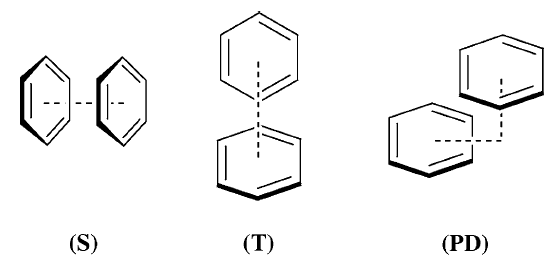
\includegraphics[scale=0.8]{image/Prot} 
		\caption[Structures du dimère de Benzène]{Structures possibles des dimères de benzène : (S) Sandwich, (T) En forme de T et (PD) Parallèle Déplacé} \label{figprot}
	\end{figure}
	
	L’analyse de ces travaux montre que le débat visant à déterminer la conformation la plus stable est loin d’être clos. La majorité des travaux annoncent les formes T et PD comme les formes les plus stables. Toutefois, intuitivement, il n'est pas illogique de penser que la configuration S, dite \og en sandwich \fg, qui correspond à une superposition maximale des deux monomères et de fait à une maximisation des interactions dispersives, puisse apparaitre comme stable. La configuration parallèle déplacée est, par exemple, souvent observée dans les expériences réalisées à l’état cristallin sur des composés purement aromatiques \cite{hunter1991pi,fyfe1997synthetic,rebek1996assembly} ou dans des études visant à caractériser les interactions des chaînes latérales aromatiques de protéines \cite{hunter1991pi,burley1985aromatic}. Klemperer \textit{et al.} \cite{janda1975benzene} ont, quant à eux, rapporté que la configuration en T était prédominante à l’état gazeux. D’autres travaux, par Arunan et Gutowsky \cite{arunan1993rotational}, issus de l'analyse des spectres rotationnels et en accord avec les études Raman de Henson \textit{et al.} \cite{henson1992raman}, rapportent que les structures favorables du dimère de benzène s’approchent de la conformation T sans pour autant la confirmer.\\ 
	
		\begin{table}[H]
			\caption{Energies d'interaction (en kcal/mol) du dimère de benzène calculées au niveau CCSD(T) et DFT-SAPT (PBE0)} \label{table-benprot}
			\begin{center}
				\begin{tabular}{l c r r r c r r c r r r}
					\toprule
					& & & \multicolumn{2}{p{2cm}}{\centering S}  &	& \multicolumn{2}{p{2cm}}{\centering
						T}& &\multicolumn{3}{p{3cm}}{\centering PD}\\
					\cline{4-12}
					& & & & R & &  &  R & & & R$_{1}$ & R$_{2}$ \\
					\midrule
					Park et Lee$^{1}$ & & & &  & &-2,67& 5,0 & &-3,03 & 3,5 & 1,8\\
					Tsuzuki et al$^{2}$ & & & -1,48& 3,8 &  &-2,46& 5,0&  & -2,48 & 3,5& 1,8\\
					Sinnokrot et al$^{3}$ & & & -1,81 & 3.8 & &-2,74& 5,0&  & -2,78 & 3,4 & 1,6\\
					Hobza et al$^{4}$ & & &-1,12 & 4.1 &  &-2,17& 5,1& & -2,01 & 3,6 & 1.8\\
					Sherrill et al$^{5}$& &  & -1,65 & 3,9 & & -2,69& 5,0 & & -2,67 & 3,5 & 1,7 \\
					Rocca$^{6}$ & & & -1,06& 3,9& & -2,15& 5,0 & & -1,82 & 3,4 & 1,8\\ 
					DFT-SAPT (PBE0)$^{7}$ & & & -1,47 & 3.9 &  &-2,44 &5,0& & -2,35& 3,5 &1,7\\
					\bottomrule
				\end{tabular}
			\end{center}
			\centering
			\footnotemark[1]{ref \cite{park2006accurate}}, CCSD(T)/CBS,
			\footnotemark[2]{ref \cite{tsuzuki2002origin}}, CCSD(T)/CBS,
			\footnotemark[3]{ref \cite{sinnokrot2002estimates}}, CCSD(T)/CBS,
			\footnotemark[4]{ref \cite{hobza1996potential}}, CCSD(T)/aug-cc-pVDZ
			\footnotemark[5]{ref \cite{sherrill2009assessment}}, CCSD(T)/CBS,
			\footnotemark[6]{ref \cite{rocca2014random}}, RPA, 
			\footnotemark[7]{SAPT(PBE0)/aug-cc-pVTZ (notre travail)}
			
			\label{benzene}
		\end{table}
		
	Il existe dans la littérature une très grande variété d’approches théoriques concernant l’étude des dimères du benzène. Nous faisons le choix de ne reporter, dans le tableau ci-dessous, que les modélisations conduisant aux résultats faisant référence, jugés \textit{a priori} comme les plus précis du fait des méthodes employées. Les travaux de Park et Lee \cite{park2006accurate}, de Tsuzuki \textit{et al.} \cite{tsuzuki2002origin} et de Sinnokrot \textit{et al.} \cite{hobza1996potential} ont tous été obtenus à partir de calculs CCSD(T) avec extrapolation CBS de base (en anglais \og Complete Basis Set extrapolation \fg). Cette méthode est une technique de calcul empirique basée sur un minimum de trois calculs séparés utilisant des bases de plus en plus complètes, telles que les bases de type cc-pVXZ (X=T, Q, 5 …). Ceci revient à obtenir une estimation approchée du résultat que l'on obtiendrait en utilisant une base de dimensions infinies. Elle permet donc d’atteindre la limite de précision de la méthode de calcul la plus performante. Nous avons reporté dans le tableau \ref{table-benprot} les résultats que nous avons obtenu, entre autre, sur la forme PD, cette forme nous intéressant \textit{a priori} plus spécifiquement puisqu'elle a pu être caractérisée expérimentalement à l'état solide (état dans lequel seront les structures à modéliser dans le présent travail, après extraction des données IR obtenues en photo acoustique). On peut remarquer, en accord avec toutes les données actuellement disponibles par le biais des approches SAPT, que notre valeur d’énergie d’interaction calculée au niveau SAPT(PBE0)/aug-cc-pVTZ est conforme à la valeur attendue. Sans surprise, l’approche SAPT permet donc de reproduire avec une excellente vélocité les énergies d’interaction de systèmes en interaction $\pi-\pi$ et d’atteindre la précision nécessaire pour reproduire des variations aussi faibles que 1 à 2 kcal/mol.
	

	
	
	
	
	
	
	\newpage
	%%%%%%%%%%%%%%%%%%%%%%%%%%%%%%%%%%%%%%%%%%%%%%
	%%%%%%%%%%%%%%%%%%%%%%%%%%%%%%%%%%%%%%%%%%%%%%
	%%%%%%%%%%%%%%%%%%%%%%%%%%%%%%%%%%%%%%%%%%%%%%
	%%%%%%%%%%%%%%%%%%%%%%%%%%%%%%%%%%%%%%%%%%%%%%
	\section{De la nécessité de la DFT}
	%%%%%%%%%%%%%%%%%%%%%%%%%%%%%%%%%%%%%%%%%%%%%%
	%%%%%%%%%%%%%%%%%%%%%%%%%%%%%%%%%%%%%%%%%%%%%%
	%%%%%%%%%%%%%%%%%%%%%%%%%%%%%%%%%%%%%%%%%%%%%%
	%%%%%%%%%%%%%%%%%%%%%%%%%%%%%%%%%%%%%%%%%%%%%%
	
	Dans ce chapitre, nous rappellerons dans un premier temps les fondements de la théorie de la fonctionnelle de la densité, abrégée en DFT, par le biais de l'évolution des différents modèles qui ont été proposés. Nous verrons ensuite comment les théorèmes de Hohenberg et Kohn prouvent que la seule connaissance de la densité électronique permet de résoudre l'équation de Schr\"{o}dinger dans le cadre de la DFT. La fonctionnelle universelle $F_{HK}[\rho]$, qui permettrait une résolution exacte du problème, restant inconnue, nous aborderons dans une troisième sous-partie l'approche KS qui contourne ce problème et légitime certaines approximations. Ces dernières donnant naissance à différents types de fonctionnelles. Après une présentation succincte, nous introduirons la notion de fonctionnelle hybride puis détaillerons le principe des approches qui ajoutent \textit{ad hoc} à un calcul KS usuel des fonctions semi-empiriques rendant compte des effets de dispersion.
	
	%%%%%%%%%%%%%%%%%%%%%%%%%%%%%%%%%%%%%%%%%%%%%%
	%%%%%%%%%%%%%%%%%%%%%%%%%%%%%%%%%%%%%%%%%%%%%%
	%%%%%%%%%%%%%%%%%%%%%%%%%%%%%%%%%%%%%%%%%%%%%%
	\subsection{Les fondements de la DFT}
	%%%%%%%%%%%%%%%%%%%%%%%%%%%%%%%%%%%%%%%%%%%%%%
	%%%%%%%%%%%%%%%%%%%%%%%%%%%%%%%%%%%%%%%%%%%%%%
	%%%%%%%%%%%%%%%%%%%%%%%%%%%%%%%%%%%%%%%%%%%%%%
	
	Contrairement aux méthodes Hartree-Fock (HF), et \textit{a fortiori} post-HF, qui décrivent le système électronique par une fonction d'onde $\Psi_{(\vec{r})}$, la théorie de la fonctionnelle de la densité le décrit par la densité électronique, notée $\rho_{(\vec{r})}$, qui est liée à la fonction d'onde $\Psi_{(\vec{r})}$ par la relation suivante~:
	
	\begin{align}
	\rho_{(\vec{r})} &= \int \Psi_{(\vec{r})}^{*} \Psi_{(\vec{r})} \\
	&= \int |\Psi_{(\vec{r})}^{2}| \notag
	\end{align}
	
	\begin{flushleft}
		\begin{tabular}{@{}lrp{10cm}}
			avec & $\vec{r}$ : & ensemble des coordonnées électroniques. 
		\end{tabular}
	\end{flushleft}
	
	
	L'énergie de l'état fondamental est ainsi une fonctionnelle de la densité électronique, c'est-à-dire que $E_{0} = E_{(\rho)}$.
	
	%%%%%%%%%%%%%%%%%%%%%%%%%%%%%%%%%%%%%%%%%%%%%%
	%%%%%%%%%%%%%%%%%%%%%%%%%%%%%%%%%%%%%%%%%%%%%%
	\subsubsection{Modèle de \textsc{Thomas-Fermi}}
	%%%%%%%%%%%%%%%%%%%%%%%%%%%%%%%%%%%%%%%%%%%%%%
	%%%%%%%%%%%%%%%%%%%%%%%%%%%%%%%%%%%%%%%%%%%%%%
	
	Le terme d'énergie cinétique a été exprimé comme une fonctionnelle de la densité pour la première fois en 1927 par Thomas et Fermi:
	
	\begin{equation}
	\hat{T}_{TF}[\rho] = \frac{3}{10} (3\pi)^{2/3} \int \rho_{(\vec{r})}^{5/3} .d\vec{r}
	\label{ener_cin_thom_ferm}
	\end{equation}
	
	Cette fonctionnelle est alors combinée aux expressions classiques des interactions électron-noyau et électron-électron, exprimées elles aussi en fonction de la densité électronique :
	
	\begin{equation}
	E_{TH}[\rho] = T_{TH}[\rho] + V_{Ne}[\rho] + V_{ee}[\rho]
	\end{equation}
	
	%%%%%%%%%%%%%%%%%%%%%%%%%%%%%%%%%%%%%%%%%%%%%%
	%%%%%%%%%%%%%%%%%%%%%%%%%%%%%%%%%%%%%%%%%%%%%%
	\subsubsection{Modèle de \textsc{Thomas-Fermi-Dirac}}
	%%%%%%%%%%%%%%%%%%%%%%%%%%%%%%%%%%%%%%%%%%%%%%
	%%%%%%%%%%%%%%%%%%%%%%%%%%%%%%%%%%%%%%%%%%%%%%
	
	Le terme d'échange, résultant du principe d'exclusion de Pauli, a été ajouté par Dirac en 1930 afin d'affiner le modèle :
	
	\begin{align}
	K[\rho] = E_{x}[\rho] &= \int \rho_{\vec{r}} \epsilon_{x}[\rho] .d\vec{r} \\
	&= -\frac{3}{4} \left(\frac{3}{\pi}\right)^{1/3} \int \rho_{(\vec{r})}^{4/3} .d\vec{r} \notag
	\end{align}
	
	\begin{flushleft}
		\begin{tabular}{@{}lrp{10cm}}
			avec & $\epsilon_{X}[\rho]$ : & énergie d'échange par électron. 
		\end{tabular}
	\end{flushleft}
	
	Le modèle de Thomas-Fermi-Dirac est défini par la combinaison de cette expression avec l'équation~\ref{ener_cin_thom_ferm} et le potentiel d'interaction électrons-noyaux $V_{Ne}[\rho]$. 
	
	
	%%%%%%%%%%%%%%%%%%%%%%%%%%%%%%%%%%%%%%%%%%%%%%
	%%%%%%%%%%%%%%%%%%%%%%%%%%%%%%%%%%%%%%%%%%%%%%
	\subsection{Modèle de \textsc{Slater}}
	%%%%%%%%%%%%%%%%%%%%%%%%%%%%%%%%%%%%%%%%%%%%%%
	%%%%%%%%%%%%%%%%%%%%%%%%%%%%%%%%%%%%%%%%%%%%%%
	
	Partant d'une approche basée sur la méthode HF, Slater propose en 1951 de substituer le terme d'énergie d'échange par une fonctionnelle de la densité issue de l'énergie d'échange de Dirac. Ce terme d'échange dans le formalisme HF peut être généralisé en introduisant le paramètre $\alpha$ :
	
	\begin{equation}
	E_{x}[\rho] = - \frac{9\alpha}{8} \left(\frac{3}{\pi}\right)^{1/3} \int \rho_{(\vec{r})}^{4/3} .d\vec{r}
	\end{equation}
	
	Des analyses empiriques basées sur différents types de systèmes chimiques ont conduit à une valeur de $3/4$ pour $\alpha$, offrant une meilleure précision que la valeur originelle de l'expression de Dirac ($2/3$).
	
	%%%%%%%%%%%%%%%%%%%%%%%%%%%%%%%%%%%%%%%%%%%%%%
	%%%%%%%%%%%%%%%%%%%%%%%%%%%%%%%%%%%%%%%%%%%%%%
	%%%%%%%%%%%%%%%%%%%%%%%%%%%%%%%%%%%%%%%%%%%%%%
	\subsection{Les théorèmes de \textsc{Hohenberg} et \textsc{Kohn}}
	%%%%%%%%%%%%%%%%%%%%%%%%%%%%%%%%%%%%%%%%%%%%%%
	%%%%%%%%%%%%%%%%%%%%%%%%%%%%%%%%%%%%%%%%%%%%%%
	%%%%%%%%%%%%%%%%%%%%%%%%%%%%%%%%%%%%%%%%%%%%%%
	
	Tous ces modèles, bien qu'ils constituent les fondements de la DFT, ne démontrent pas formellement que seule la connaissance de la densité est importante pour accéder à l'énergie totale d'un système. C'est ainsi que Hohenberg et Kohn eurent l'idée, en 1965, de démontrer, par le biais de deux théorèmes, que l'équation de Schr\"{o}dinger pouvait être résolue de façon exacte dans le cadre de l'approximation de Born-Oppenheimer, uniquement grâce à la densité électronique.
	
	%%%%%%%%%%%%%%%%%%%%%%%%%%%%%%%%%%%%%%%%%%%%%%
	%%%%%%%%%%%%%%%%%%%%%%%%%%%%%%%%%%%%%%%%%%%%%%
	\subsubsection{Premier théorème : preuve d'existence}
	%%%%%%%%%%%%%%%%%%%%%%%%%%%%%%%%%%%%%%%%%%%%%%
	%%%%%%%%%%%%%%%%%%%%%%%%%%%%%%%%%%%%%%%%%%%%%%
	
	Ce premier théorème énonce que l'ensemble des propriétés du système, notamment l'énergie, peuvent être calculées à partir de la seule densité électronique de l'état fondamental. Elles peuvent donc être décrites comme une fonctionnelle de la densité électronique, et l'énergie totale s'écrit :
	
	\begin{equation}
	E[\rho] = F_{HK}[\rho] + \int \rho_{(\vec{r})} \nu_{ext} .d\vec{r}
	\label{Hohen_Kohn}
	\end{equation}
	\noindent où :
	\begin{align}
	F_{HK}[\rho] &= T_{e}[\rho] + V_{ee}[\rho] \\
	\nu_{ext} &= V_{Ne}[\rho] \notag
	\end{align}
	
	Notons que la fonctionnelle universelle $F_{HK}[\rho]$, qui regroupe les termes d'énergie cinétique des électrons et celui d'énergie potentielle d'interaction électron-électron, n'est pas liée au potentiel externe $\nu_{ext}$. L'énergie de l'état fondamental est \textit{a priori} accessible de manière exacte car cette fonctionnelle ne repose sur aucune approximation.
	
	%%%%%%%%%%%%%%%%%%%%%%%%%%%%%%%%%%%%%%%%%%%%%%
	%%%%%%%%%%%%%%%%%%%%%%%%%%%%%%%%%%%%%%%%%%%%%%
	\subsubsection{Second théorème : théorème variationnel}
	%%%%%%%%%%%%%%%%%%%%%%%%%%%%%%%%%%%%%%%%%%%%%%
	%%%%%%%%%%%%%%%%%%%%%%%%%%%%%%%%%%%%%%%%%%%%%%
	
	Basé sur l'équation~\ref{Hohen_Kohn}, Hohenberg et Kohn ont ensuite établi un principe variationnel pour déterminer la densité électronique de l'état fondamental :
	
	\begin{equation}
	E[\rho] \geq E[\rho_{0}]
	\end{equation}
	
	\begin{flushleft}
		\begin{tabular}{@{}lrp{10cm}}
			avec & $\rho_{0}$ : & densité électronique de l'état fondamental, \\
			& $\rho$ : & densité électronique quelconque.
		\end{tabular}
	\end{flushleft}
	
	Dans cette équation, à une densité d'essai $\rho$ correspond une seule énergie potentielle $\int \rho_{(\vec{r})} \nu_{ext} .d\vec{r}$ et une seule fonction d'onde $\Psi_{\rho}$. La méthode de double minimisation, \textit{i.e.} sous contrainte de Levy, permet de différencier la fonction d'onde $\Psi_{\rho_{0}}$, correspondant à l'état fondamental, parmi le jeu infini des fonctions d'ondes $\Psi_{\rho}$ donnant la même densité. Ainsi, nous pouvons déterminer, parmi toutes les densités, celle qui minimisera l'énergie par la relation suivante :
	
	\begin{equation}
	E[\rho_{0}] = \min\limits_{\rho}\, (\min\limits_{\Psi\rightarrow\rho}\, (F[\rho] + \int \rho_{\vec{r}} \nu_{\vec{r}}\, .d\vec{r}\, ))
	\end{equation}
	
	Si les théorèmes de Hohenberg et Kohn démontrent une correspondance unique entre une densité $\rho_{\vec{r}}$ et la fonction d'onde $\Psi$ du système, la fonctionnelle universelle $F_{HK}[\rho]$ reste cependant inconnue.
	
	%%%%%%%%%%%%%%%%%%%%%%%%%%%%%%%%%%%%%%%%%%%%%%
	%%%%%%%%%%%%%%%%%%%%%%%%%%%%%%%%%%%%%%%%%%%%%%
	%%%%%%%%%%%%%%%%%%%%%%%%%%%%%%%%%%%%%%%%%%%%%%
	\subsection{Approche Kohn-Sham}\label{Kohn-Sham}
	%%%%%%%%%%%%%%%%%%%%%%%%%%%%%%%%%%%%%%%%%%%%%%
	%%%%%%%%%%%%%%%%%%%%%%%%%%%%%%%%%%%%%%%%%%%%%%
	%%%%%%%%%%%%%%%%%%%%%%%%%%%%%%%%%%%%%%%%%%%%%%
	
	Afin de contourner ce problème, Kohn et Sham substituèrent au Hamiltonien réel, décrivant un système de $n$ particules en interaction, un Hamiltonien de référence décrivant un système de $n$ particules sans interaction mais ayant la même densité que le système réel. Le problème est ainsi réduit à la résolution de $n$ équations monoélectronique couplées, analogues aux équations HF. L'opérateur monoélectronique de Kohn-Sham $\hat{K}_{KS}$ s'exprime ainsi :
	
	\begin{equation}
	\hat{H}_{KS} = -\frac{1}{2} \nabla^{2} + \nu_{H}[\rho] + \nu_{xc}[\rho] + \nu_{ext}[\rho]
	\end{equation}
	
	\noindent où :
	\begin{align}
	\nu_{H}[\rho] &= \int \frac{\rho_{(\vec{r})} - \rho_{(\vec{r}')}}{|\vec{r} - \vec{r}'|} .d\vec{r}' \\
	\nu_{xc}[\rho] &= \frac{\partial E_{xc}[\rho_{(\vec{r})}]}{\partial\rho_{(\vec{r})}}
	\end{align}
	
	\noindent $\nu_{H}[\rho]$ et $\nu_{xc}[\rho]$ étant respectivement le potentiel de Hartree et le potentiel d'échange et de corrélation, dans lequel $E_{xc}[\rho_{(\vec{r})}]$ est l'énergie d'échange et de corrélation.
	
	En définissant un potentiel fictif $\nu_{eff(\vec{r})}$ pouvant être appliqué à des systèmes sans interaction de densité $\rho$ :
	
	\begin{equation}
	\nu_{eff(\vec{r})} = \nu_{H}[\rho] + \nu_{xc}[\rho] + \nu_{ext}[\rho]
	\end{equation}
	
	\noindent nous introduisons un jeu d'orbitales $\psi_{(\vec{r})}$, appelées orbitales de Kohn-Sham, et nous obtenons un jeu d'équations aux valeurs propres :
	
	\begin{equation}
	\hat{H}_{KS} \psi_{i(\vec{r})} = \epsilon_{i} \psi_{i(\vec{r})}
	\end{equation}
	
	Comme dans le cas de la méthode HF, l'énergie du système peut être minimisée en résolvant ce jeu d'équations de façon auto-cohérente grâce à l'utilisation des orbitales de Kohn-Sham. L'énergie du système est alors donnée par :
	
	\begin{equation}
	E_{KS}^{tot}[\rho] = T_{s}[\rho] + J[\rho] + E_{xc}[\rho] + \int V_{ext(\vec{r})}\rho_{(\vec{r})} .d\vec{r}
	\end{equation}
	
	\begin{flushleft}
		\begin{tabular}{@{}lrp{10cm}}
			avec & $T_{s}[\rho]$ : & énergie cinétique des électrons sans interaction, \\
			& $J[\rho]$ : & énergie d'interaction coulombienne entre les électrons, \\
			& $E_{xc}[\rho]$ : & énergie d'échange et de corrélation, \\
			& $\int V_{ext(\vec{r})}\rho_{(\vec{r})} .d\vec{r}$ : & énergie d'interaction avec le potentiel externe. 
		\end{tabular}
	\end{flushleft}
	
	D'après les théorèmes de Hohenberg et Kohn, $E_{KS}^{tot}[\rho]$ doit être égale à l'énergie totale du système réel $E_{reel}^{tot}[\rho]$, qui peut être décrite comme suit :
	
	\begin{equation}
	E_{reel}^{tot}[\rho] = T[\rho] + V_{ee}[\rho] + \int V_{ext(\vec{r})}\rho_{(\vec{r})} .d\vec{r}
	\end{equation}
	
	Le terme d'échange-corrélation peut ainsi être explicité comme la somme de la correction à l'énergie cinétique due à l'interaction entre électrons ($T[\rho] - T_{s}[\rho]$) et des corrections non classiques à la répulsion électron-électron ($V_{ee}[\rho] - J[\rho]$) :
	
	\begin{equation}
	E_{xc}[\rho] = T[\rho] - T_{s}[\rho] + V_{ee}[\rho] - J[\rho]
	\end{equation}
	
	La théorie de la fonctionnelle de la densité de Kohn-Sham (KS) a connu un grand succès parmi les méthodes de calcul appliquées aux systèmes de grande dimension, du fait de son ratio coût calculatoire/performance très intéressant. C'est pour cet avantage indéniable qu'elle sert de base à de nombreuses évolutions de la DFT.
	
	%%%%%%%%%%%%%%%%%%%%%%%%%%%%%%%%%%%%%%%%%%%%%%
	%%%%%%%%%%%%%%%%%%%%%%%%%%%%%%%%%%%%%%%%%%%%%%
	%%%%%%%%%%%%%%%%%%%%%%%%%%%%%%%%%%%%%%%%%%%%%%
	\subsection{Les différentes classes de fonctionnelles}
	%%%%%%%%%%%%%%%%%%%%%%%%%%%%%%%%%%%%%%%%%%%%%%
	%%%%%%%%%%%%%%%%%%%%%%%%%%%%%%%%%%%%%%%%%%%%%%
	%%%%%%%%%%%%%%%%%%%%%%%%%%%%%%%%%%%%%%%%%%%%%%
	
	Formellement, la DFT est donc une méthode exacte, dans la limite de la connaissance de la fonctionnelle universelle $F_{HK}[\rho]$ ou de sa fonctionnelle exacte d’échange et de corrélation $F_{xc}[\rho]$. Malheureusement, la forme exacte de l’énergie d’échange et de corrélation est inconnue, si bien qu’il est nécessaire de faire des approximations. Dans la pratique, l’énergie d’échange et de corrélation $E_{xc}[\rho]$ est calculée à l’aide de fonctionnelles d’échange et de corrélation définies comme suit :
	
	\begin{equation}
	\int F_{xc}[\rho_{(\vec{r})}].d\vec{r} = E_{xc}[\rho_{(\vec{r})}]
	\end{equation}
	
	L’énergie d’échange et de corrélation est généralement séparée en deux termes distincts, l’un d’échange -- $E_{x}[\rho]$ -- et l’autre de corrélation -- $E_{c}[\rho]$ :
	
	\begin{equation}
	E_{xc}[\rho_{(\vec{r})}] = E_{x}[\rho_{(\vec{r})}] + E_{c}[\rho_{(\vec{r})}]
	\end{equation}
	
	Plusieurs fonctionnelles ont donc été développées pour traiter chacune de ces contributions, de façon simultanée ou indépendante. Nous allons ici donner un bref aperçu -- non exhaustif -- des différentes familles de fonctionnelles, en suivant le critère de classification élaboré par Perdew et couramment appelé \og échelle de Perdew \fg{}. Il a proposé de classer les fonctionnelles en fonction du degré d’informations non locales contenues dans leur forme analytique. Au premier échelon se trouvent les fonctionnelles qui dépendent uniquement de la densité électronique, dites fonctionnelles LDA (\og Local Density Approximation \fg{}). Viennent ensuite les fonctionnelles corrigées par gradient, dites GGA (\og Generalized Gradient Approximation \fg{}), dans lesquelles la non-localité est introduite grâce à leur dépendance vis-à-vis du gradient de la densité. A ce même niveau se trouvent également les fonctionnelles de type méta-GGA, dépendant aussi de l’énergie cinétique (calculée à partir des orbitales moléculaires remplies). Il faut noter que, d’un point de vue mathématique, toutes ces familles de fonctionnelles sont strictement locales. Pour parvenir à des fonctionnelles véritablement non locales, il faut encore monter d’un cran dans l’échelle de Perdew, jusqu’aux fonctionnelles dites hybrides, où la présence d’un pourcentage (variable) d’échange HF calculé en utilisant les orbitales KS, permet d’introduire un véritable terme non local. Plus récemment une autre famille de fonctionnelles hybrides a été développée (dite à longue portée ou encore à séparation de portée) dans laquelle le pourcentage d’échange calculé de façon HF n’est pas constant mais dépend de la distance inter-électronique. Enfin, des fonctionnelles non locales montrant une dépendance explicite des orbitales KS occupées et vacantes représentent le dernier niveau dans l’échelle de Perdew.
	
	%%%%%%%%%%%%%%%%%%%%%%%%%%%%%%%%%%%%%%%%%%%%%%
	%%%%%%%%%%%%%%%%%%%%%%%%%%%%%%%%%%%%%%%%%%%%%%
	\subsubsection{Local Density approximation (LDA)}\label{lda}
	%%%%%%%%%%%%%%%%%%%%%%%%%%%%%%%%%%%%%%%%%%%%%%
	%%%%%%%%%%%%%%%%%%%%%%%%%%%%%%%%%%%%%%%%%%%%%%
	
	L’approximation locale de la densité est l’approximation la plus grossière, dans laquelle l’énergie d’échange et de corrélation $E_{xc}$ n’est fonction que de la seule densité électronique :
	
	\begin{equation}
	E_{xc}^{LDA}[\rho_{(\vec{r})}] = \int \rho_{(\vec{r})} \epsilon_{xc}[\rho_{(\vec{r})}].d\vec{r}
	\end{equation}
	
	\noindent où la valeur de $\epsilon_{xc}$ à une position $\vec{r}$ est calculée exclusivement à partir de la valeur de la densité électronique $\rho$ à cette position. En pratique, $\epsilon_{xc}$ décrit l’énergie d’échange et de corrélation par particule pour un gaz uniforme d’électrons de densité $\rho$. Le potentiel d’échange et de corrélation correspondant est alors :
	
	\begin{equation}
	\nu_{xc(\vec{r})}^{LDA} = \epsilon_{xc}[\rho_{(\vec{r})}] + \rho_{(\vec{r})} \frac{\partial \epsilon_{xc}[\rho_{(\vec{r})}]}{\partial \rho}
	\end{equation}
	
	Malgré le fait que les résultats obtenus soient généralement en bon accord avec les résultats expérimentaux, notamment au niveau de la géométrie et de la structure électronique, cette approximation reste une approximation locale, dans laquelle il n'est pas tenu compte de l’inhomogénéité de la densité électronique.
	
	%%%%%%%%%%%%%%%%%%%%%%%%%%%%%%%%%%%%%%%%%%%%%%
	%%%%%%%%%%%%%%%%%%%%%%%%%%%%%%%%%%%%%%%%%%%%%%
	\subsubsection{Generalized Gradient Approximation (GGA)}
	%%%%%%%%%%%%%%%%%%%%%%%%%%%%%%%%%%%%%%%%%%%%%%
	%%%%%%%%%%%%%%%%%%%%%%%%%%%%%%%%%%%%%%%%%%%%%%
	
	L’idée directrice de l’approximation du gradient généralisé est donc de mieux tenir compte de l’inhomogénéité de la densité du système, en introduisant une dépendance de la densité $\rho$ à son gradient $\nabla \rho$. L’expression générale des fonctionnelles de type GGA est la suivante :
	
	\begin{equation}
	E_{xc}^{GGA}[\rho_{(\vec{r})}] = A_{x} \int \rho_{(\vec{r})}^{4/3} E^{GGA}(s) .d\vec{r}^{3}
	\end{equation}
	
	\noindent où $s$, gradient de la densité réduite, est tel que :
	
	\begin{equation}
	s = \frac{|\nabla \rho_{(\vec{r})}|}{2 k_{F} \rho_{(\vec{r})}}
	\end{equation}
	
	\noindent avec $k_{F} = (3 \pi^{2} \rho_{(\vec{r})})^{1/3}$. Ainsi, on fait apparaître par le biais du terme $s$ un terme quasi-local, dépendant non seulement de la densité électronique mais également de son gradient au voisinage de $\vec{r}$.
	
	Un exemple de fonctionnelle GGA est celle de Perdew, Burke et Ernzherhof, notée PBE~\cite{perdew1996generalized}.
	
	%%%%%%%%%%%%%%%%%%%%%%%%%%%%%%%%%%%%%%%%%%%%%%
	%%%%%%%%%%%%%%%%%%%%%%%%%%%%%%%%%%%%%%%%%%%%%%
	\subsubsection{Fonctionnelles hybrides}
	%%%%%%%%%%%%%%%%%%%%%%%%%%%%%%%%%%%%%%%%%%%%%%
	%%%%%%%%%%%%%%%%%%%%%%%%%%%%%%%%%%%%%%%%%%%%%%
	
	La dernière grande famille de fonctionnelles est celle des fonctionnelles hybrides. L’idée consiste à introduire une fraction d’échange calculée de façon exacte (telle qu’utilisée dans la méthode HF) dans une fonctionnelle d’échange de type GGA. L’expression de $E_{xc}$ devient alors :
	
	\begin{equation}
	E_{xc}^{hybride}[\rho_{(\vec{r})}] = (1- \alpha) E_{xc}^{GGA}[\rho_{(\vec{r})}] + \alpha E_{xc}^{HF}[\rho_{(\vec{r})}]
	\end{equation}
	
	\noindent où le coefficient de la combinaison $\alpha$ donne le rapport HF/DFT. \\
	La fonctionnelle PBE0~\cite{adamo1999toward}, par exemple, présente 25\% d’échange HF~\cite{adamo1997toward} dans une fonctionnelle GGA de type PBE~\cite{perdew1996generalized} :
	
	\begin{equation}
	E_{xc}^{PBE0} = E_{xc}^{PBE} + \frac{1}{4} (E_{x}^{HF} - E_{x}^{PBE})
	\end{equation}
	
	Elle a l’avantage d’être non paramétrée (car le pourcentage d’HF inclus n’est pas empirique mais basé sur des arguments de théorie perturbationnelle), et de fournir des résultats très précis, tant au niveau du calcul des structures moléculaires et électroniques que pour le calcul de propriétés spectroscopiques \cite{adamo1999toward}.
	
	Dans cette catégorie figure également la fonctionnelle la plus utilisée pour traiter des systèmes moléculaires, à savoir la fonctionnelle B3LYP \cite{becke1993density}. Comme son nom l’indique, elle inclus trois paramètres et se base sur les fonctionnelles GGA d’échange et de corrélation de Becke (B) \cite{becke1988density} et Lee, Yang et Parr (LYP) \cite{chengteh1988development}, suivant l’expression :
	
	\begin{equation}
	E_{xc}^{B3LYP} = (1-a) E_{x}^{LSDA} + a E_{x}^{HF} + b \Delta E_{x}^{B} + (1-c) E_{c}^{LSDA} + c E_{c}^{LYP}
	\label{B3LYP}
	\end{equation}
	
	\noindent avec $a$, $b$ et $c$ fixés respectivement à 0,20 , 0,72 et 0,81.
	
	
	%%%%%%%%%%%%%%%%%%%%%%%%%%%%%%%%%%%%%%%%%%%%%%
	%%%%%%%%%%%%%%%%%%%%%%%%%%%%%%%%%%%%%%%%%%%%%%
	\subsubsection{Nécessité d'une fonctionnelle « longue portée »}
	%%%%%%%%%%%%%%%%%%%%%%%%%%%%%%%%%%%%%%%%%%%%%%
	%%%%%%%%%%%%%%%%%%%%%%%%%%%%%%%%%%%%%%%%%%%%%%
	
	Bien que la théorie de la fonctionnelle de la densité connaisse un large succès, elle conduit toujours à des écueils dès lors que l'on tente de l'employer pour l'étude de systèmes chimiques où les forces de van der Waals sont prédominantes. 
	En effet, les effets de corrélation électronique des forces de dispersion étant purement non-locaux, l'approximation locale ou non-locale qui fait le fondement de la DFT reste problématique. Se pose alors la question de savoir comment modéliser uniformément ces interactions.
	 Comme nous allons l'expliciter, les fonctionnelles hybrides dites \og à longue portée \fg{} permettent de répondre, au premier degré de l'échelle de précision, à cette problématique. 
	
	
	%%%%%%%%%%%%%%%%%%%%%%%%%%%%%%%%%%%%%%%%%%%%%%
	%%%%%%%%%%%%%%%%%%%%%%%%%%%%%%%%%%%%%%%%%%%%%%
	%%%%%%%%%%%%%%%%%%%%%%%%%%%%%%%%%%%%%%%%%%%%%%
	\subsection[LC-DFT-D hybride : $\omega$BXD]{Construction d'une LC-DFT-D hybride : cas de la $\omega$BXD}
	%%%%%%%%%%%%%%%%%%%%%%%%%%%%%%%%%%%%%%%%%%%%%%
	%%%%%%%%%%%%%%%%%%%%%%%%%%%%%%%%%%%%%%%%%%%%%%
	%%%%%%%%%%%%%%%%%%%%%%%%%%%%%%%%%%%%%%%%%%%%%%
	Les fonctionnelles hybrides avec correction à longue portée basées sur la théorie Kohn-Sham ont naturellement rencontré un grand engouement puisque la précision apportée n'accroît pas le coût calculatoire par comparaison aux méthodes DFT hybrides.
	
	%%%%%%%%%%%%%%%%%%%%%%%%%%%%%%%%%%%%%%%%%%%%%%
	%%%%%%%%%%%%%%%%%%%%%%%%%%%%%%%%%%%%%%%%%%%%%%
	\subsubsection{B88}
	%%%%%%%%%%%%%%%%%%%%%%%%%%%%%%%%%%%%%%%%%%%%%%
	%%%%%%%%%%%%%%%%%%%%%%%%%%%%%%%%%%%%%%%%%%%%%%
	
	Comme nous l'avons vu dans le cadre des approximations de la fonctionnelle de la densité \footnote{\og Density Functional Approximations \fg{} }, notées DFAs, la décroissance exponentielle du potentiel d'échange-corrélation engendre une mauvaise représentation des interactions à longue distance, qui varient quant à elles en $1/r$. Cette erreur, baptisée erreur d'auto-interaction (ou SIE, pour \og self-interaction error \fg{}), est liée au fait que ces approximations se basent sur la densité de spin locale (LSDA, pour \og local spin density approximation \fg{}). De fait, elles décrivent mal l'état fondamental qui devrait être, dans le cadre de la DFT pure, strictement sans auto-interaction.     
	C'est pourquoi, afin d'introduire un effet non-local de l'échange-corrélation dans le modèle KS-DFT (partie~\ref{Kohn-Sham}), Becke proposa en 1988 d'incorporer dans sa fonctionnelle d'échange B88~\cite{becke1988density} une fraction d'échange calculée de façon exacte Hartree-Fock. 
	
	Dans le cadre général des DFAs, l'énergie d'échange-corrélation s'écrit donc :
	
	\begin{equation}
	E_{xc} = c_{x}E_{x}^{HF} + E_{xc}^{DFA}
	\label{xcB88}
	\end{equation}
	
	\noindent où $c_{x}$ prend généralement des valeurs comprises entre 0,2 et 0,25~\cite{becke1993density} pour traduire au mieux les propriétés thermodynamiques, et entre 0,4 et 0,6~\cite{boese2004development} pour traduire au mieux les données cinétiques.
	
	Basée sur ce modèle, la désormais bien connue DFT hybride B3LYP \cite{becke1993density} (équation~\ref{B3LYP}) donne des résultats comparables à ceux obtenus à partir de la théorie perturbative M\o ller-Plesset à l'ordre 2 \cite{moller1934note} (MP2), souvent utilisée comme référence, dans le cadre de systèmes fortement liés. Depuis, de nombreuses recherches ont porté sur l'amélioration constante de ce potentiel d'échange-corrélation $E_{xc}[\rho]$.
	
	À ce stade, il me paraît essentiel de rappeler le caractère quelque peu \og erratique \fg{} des résultats de nombre de travaux menés en DFT, caractère qui tient au choix de la fonctionnelle d'échange et/ou de corrélation. 
	 Lorsque, pour un système donné, une fonctionnelle d’échange-corrélation se révèle capable de traduire des paramètres physiques avec une précision satisfaisante autour de la position d’équilibre, rien ne garantit qu’elle soit en mesure de donner la même précision pour un autre (type de) système(s). Il en va de même pour l’étude de dimères (atomiques ou moléculaires). Dans le présent travail, une attention toute particulière a donc été portée au choix de la fonctionnelle d’échange-corrélation, s'agissant d'une étude portant sur une très grande variété de systèmes, \textit{i.e.} non seulement des familles de molécules comportant un ou plusieurs hétéroatome(s) mais les homo-dimères correspondants. La fonctionnelle $\omega$b97X a retenu notre attention dans ce travail.
	
	
	%%%%%%%%%%%%%%%%%%%%%%%%%%%%%%%%%%%%%%%%%%%%%%
	%%%%%%%%%%%%%%%%%%%%%%%%%%%%%%%%%%%%%%%%%%%%%%
	\subsubsection{B97}
	%%%%%%%%%%%%%%%%%%%%%%%%%%%%%%%%%%%%%%%%%%%%%%
	%%%%%%%%%%%%%%%%%%%%%%%%%%%%%%%%%%%%%%%%%%%%%%
	
	Une avancée significative a de nouveau été faite par Becke en 1997 dans le domaine des KS-DFT. Par une méthode similaire à la combinaison linéaire d'orbitales atomiques \footnote{\og Linear Combination of Atomic Orbitals \fg{}.}, notée LCAO, Becke a proposé un modèle mathématique basé sur l'approximation de densité de spin local (LSDA), sa première dérivée et une petite fraction d'échange HF pour décrire le potentiel d'échange-corrélation $E_{xc}[\rho]$. Une optimisation systématique des coefficients linéaires à partir d'un jeu classique de données expérimentales a conduit à l'apparition de la méthode B97~\cite{becke1997density}. La base de données contient notamment des valeurs relatives à l'interaction entre systèmes conjugués.
	
	Cette méthodologie a été reprise par F. A. Hamprecht \textit{et al.}, P. J. Wilson \textit{et al.} et T. W. Keal \textit{et al.} pour respectivement conduire à la B97-1 \cite{hamprecht1998development} (1998), la B97-2 \cite{wilson2001hybrid} (2001) et la B97-3 \cite{keal2005semiempirical} (2005). Il s'agissait alors de réoptimisations des coefficients linéaires par rapport à de nouvelles bases de données expérimentales, plus complètes.
	
	Mais cette nouvelle paramétrisation empirique du terme d'échange-corrélation ne résout pas le problème de sa non-décroissance en $1/r$. La prise en compte totale du terme d'échange HF $E_{x}^{HF}$ ($c_{x}$=1 dans l'équation~\ref{xcB88}) pourrait résoudre ce problème mais serait incompatible avec le terme de corrélation DFA $E_{c}^{DFA}$, engendrant une mauvaise compensation des erreurs respectives.
	
	%%%%%%%%%%%%%%%%%%%%%%%%%%%%%%%%%%%%%%%%%%%%%%
	%%%%%%%%%%%%%%%%%%%%%%%%%%%%%%%%%%%%%%%%%%%%%%
	\subsubsection{$\omega$B97}
	%%%%%%%%%%%%%%%%%%%%%%%%%%%%%%%%%%%%%%%%%%%%%%
	%%%%%%%%%%%%%%%%%%%%%%%%%%%%%%%%%%%%%%%%%%%%%%
	
	L'idée de séparer le traitement des interactions courtes (SR, pour \og short range \fg{}) et longues portées (LR, pour \og long range \fg{}) s'est alors présentée comme le choix le plus évident, aussi bien au niveau de la compréhension des phénomènes que sur le plan mathématique. Le principe est de traiter séparément, à l'aide d'une fonction erreur $(erf)$, les interactions à courte et à longue distance. Les interactions à courte distance sont représentées par une fonctionnelle de la densité, tandis que les interactions à longue distance sont traduites par une fonction d'onde. Ce principe conduit naturellement à l'élaboration d'une fonctionnelle hybride à séparation de portée. L'introduction de la fonction erreur, avec un paramètre libre, permet de contrôler le rayon d'action des interactions à courte portée.
	
	Iikura \textit{et al.} \cite{iikura2001long} ont été parmi les premiers à proposer ce type de solutions. Leur méthode consiste à traiter la partie d'échange (LR) par la théorie HF, tandis que la partie SR est approximée par une DFA ; le terme de corrélation est quant à lui le même que celui de Coulomb, quelle que soit la distance :
	
	\begin{equation}
	E_{xc}^{LC-DFA} = E_{x}^{LR-HF} + E_{x}^{SR-DFA} + E_{c}^{DFA}
	\end{equation}
	
	Ce schéma de séparation de portée a l'avantage de conduire à des temps de calcul très proches des DFT hybrides. Reste toutefois à développer une fonctionnelle d'échange SR précise ainsi qu'une fonctionnelle de corrélation compatible avec la fonctionnelle d'échange.
	
	Le type d'opérateur de coupure le plus utilisé dans le cadre des LC-DFT hybrides est la fonction d'erreur standard, notée $(erf)$ :
	
	\begin{equation}
	\frac{1}{r} = \frac{erf(\omega r_{12})}{r_{12}} + \frac{erfc(\omega r_{12})}{r_{12}}
	\label{erf}
	\end{equation}
	
	\begin{flushleft}
		\begin{tabular}{@{}lrp{10cm}}
			avec & $\frac{erf(\omega r_{12})}{r_{12}}$ : & interaction de courte portée, \\
			& $\frac{erfc(\omega r_{12})}{r_{12}}$ : & interaction complémentaire, \\
			& $r_{12}$ : & distance entre les particules 1 et 2, \\
			& $\omega$ : & paramètre contrôlant la séparation.
		\end{tabular}
	\end{flushleft}
	
	Dans cette équation, l'introduction du paramètre $\omega$, qui s'exprime comme l'inverse d'une distance, permet de donner un sens physique à la fonction d'erreur, puisqu'il est étroitement lié à une longueur caractéristique de la séparation.
	Naturellement, il existe différents types de fonctions erreur $(erf)$, qui facilitent son intégration mathématique dans les codes de calculs. Dans le cas de la fonctionnelle $\omega$B97 \cite{chai2008long} et de ses améliorations (à savoir les fonctionnelles $\omega$B97X et $\omega$B97X-D), c'est la fonction $erf/erfc$ qui a été choisie par Jeng-Da Chai et Martin Head-Gordon dans leurs travaux. 
	Le choix des auteurs s'est porté sur un terme d'échange exact HF longue portée $E_{x}^{LR-HF}$, calculé à partir des spin-orbitales occupées $\phi_{i \sigma}(r)$, et une forme analytique du terme d'échange $E_{x}^{SR-DFA}$ obtenue par intégration du carré de la matrice densité LSDA :
	
	\begin{align}
	E_{x}^{LR-HF} &= -\frac{1}{2} \sum_{\sigma} \sum_{ij}^{occ.} \iint \phi_{i \sigma}^{*}(r_{1}) \phi_{j \sigma}^{*}(r_{1}) \frac{erf(\omega r_{12})}{r_{12}} \phi_{i \sigma}(r_{2}) \phi_{j \sigma}(r_{2}).dr_{1}.dr_{2}, \\
	E_{x}^{SR-LSDA} &= \sum_{\sigma} \int \underbrace{-\frac{3}{2}\left(\frac{3}{4\pi}\right)^{1/3}\rho_{\sigma}^{4/3} (r) F(a_{\sigma})}_{e_{x \sigma}^{SR-LSDA} (\rho_{\sigma}) .dr}.
	\end{align}
	
	\noindent où :
	\begin{align}
	k_{F \sigma}&=(6\pi^{2}\rho_{sigma}(r))^{1/3},\nonumber\\
	F(a_{\sigma})&=1-\frac{8}{3}a_{\sigma}\left[\sqrt{\pi}\: erf\left(\frac{1}{2a_{\sigma}}\right)-3a_{\sigma}+4a_{\sigma}^{3}+(2a_{\sigma}-4a_{\sigma}^{3}) \: exp\left(-\frac{1}{4a_{\sigma}^{2}}\right)\right],\nonumber\\
	a_{\sigma}&=\frac{\omega}{2k_{F\sigma}}.\nonumber
	\end{align}
	
	\begin{flushleft}
		\begin{tabular}{@{}lrp{10cm}}
			avec & $k_{F\sigma}$ : & vecteur d'onde local de Fermi,\\
			& $F(a_{\sigma})$ : & fonction d'atténuation,\\
			& $a_{\sigma}$ : & paramètre de contrôle (sans unité) de la fonction d'atténuation $F(a_{\sigma})$.
		\end{tabular}
	\end{flushleft}
	
	En retenant une fonctionnelle de corrélation basée elle aussi sur la LSDA $E_{c}^{LSDA}$, la plus simple des DFT hybrides à correction de longue portée (RSHX-LDA pour l’anglais \og Range Separated Hybrid eXchange \fg{} \cite{angyan2005van} s'écrit~:
	
	\begin{equation}
	E_{xc}^{RSHXLDA} = E_{x}^{LR-HF} + E_{x}^{SR-LSDA} + E_{c}^{LSDA}
	\end{equation}
	
	La fonctionnelle $\omega$B97\cite{chai2008long} s'écrit alors :
	
	\begin{equation}
	E_{xc}^{\omega B97} = E_{x}^{LR-HF} + E_{x}^{SR-B97} + E_{c}^{B97}
	\end{equation}
	
	Il est à noter que celle-ci ne possède pas d'échange Hartree-Fock à courte portée (SR), comme la plupart des fonctionnelles hybrides à correction de portée.
	
	En dépit de nombreuses études visant à optimiser la valeur du paramètre $\omega$, la précision calculatoire reste insuffisante du point de vue de la thermochimie. En effet, comme nous l'avons souligné ci-avant, une valeur trop élevée du paramètre $\omega$ engendrerait une incompatibilité entre le terme d'échange non-local, $E_{x}^{LR-HF}$, et le terme local de corrélation, $E_{c}^{LSDA}$. De plus, d'après l'équation~\ref{erf}, plus $\omega$ est petit, plus la contribution du terme d'échange (SR), $E_{x}^{SR-LSDA}$, sera importante. Attribuer à $\omega$ une valeur trop faible reviendrait alors à traiter le problème dans un cadre très proche de la LDA classique qui, comme nous l'avons vu dans la partie~\ref{lda}, est incapable de traduire correctement le terme d'échange à courte portée.
	
	%%%%%%%%%%%%%%%%%%%%%%%%%%%%%%%%%%%%%%%%%%%%%%
	%%%%%%%%%%%%%%%%%%%%%%%%%%%%%%%%%%%%%%%%%%%%%%
	\subsubsection{$\omega$B97X}
	%%%%%%%%%%%%%%%%%%%%%%%%%%%%%%%%%%%%%%%%%%%%%%
	%%%%%%%%%%%%%%%%%%%%%%%%%%%%%%%%%%%%%%%%%%%%%%
	
	Afin de remédier à ce problème, une partie d'échange (SR) HF, notée $E_{x}^{SR-HF}$, est ajoutée à $E_{x}^{SR-LSDA}$ dans une proportion d'environ 16\%, de la même manière que Becke dans la fonctionnelle B88. Ceci présente l'avantage de ne pas perturber la partie LR, qui est quant à elle correcte. La nouvelle fonctionnelle comporte donc désormais un paramètre, noté $c_{x}$, contrôlant la proportion d'échange exact HF à courte distance :
	
	\begin{equation}
	E_{xc}^{LC-DFA} = E_{x}^{LR-HF} + c_{x}E_{x}^{SR-HF} + E_{x}^{SR-DFA} + E_{c}^{DFA}
	\end{equation}
	
	\noindent où :
	
	\begin{equation}
	E_{x}^{SR-HF} = -\frac{1}{2} \sum_{\sigma} \sum_{ij}^{occ.} \iint \phi_{i \sigma}^{*}(r_{1}) \phi_{j \sigma}^{*}(r_{1}) \frac{erfc(\omega r_{12})}{r_{12}} \phi_{i \sigma}(r_{2}) \phi_{j \sigma}(r_{2}).dr_{1}.dr_{2}, \\
	\end{equation}
	
	C'est ainsi que la fonctionnelle $\omega$B97X\cite{chai2008long} se décompose de la façon suivante~:
	
	\begin{equation}
	E_{xc}^{\omega B97X} = E_{x}^{LR-HF} + c_{x}E_{x}^{SR-HF} + E_{x}^{SR-B97} + E_{c}^{B97}
	\end{equation}
	
	La valeur de $\omega$ et les valeurs des coefficients de développement linéaire et de développement à l'ordre $m$ des fonctionnelles $\omega$B97 et $\omega$B97X, ont été déterminées par la méthode des moindres carrés appliquée à une base de données composées de 412 valeurs précises, expérimentales et théoriques.
	
	Malgré toutes ces optimisations conduisant à une bien meilleure représentation des systèmes en interaction, ces fonctionnelles connaissent encore des lacunes quant à la traduction des interactions de dispersion entre atomes (\textit{i.e.} les forces de London). Comme nous allons le voir dans le cas de la fonctionnelle $\omega$B97X-D, ces écueils peuvent être corrigés par une prise en compte empirique des effets de dispersion.
	
	%%%%%%%%%%%%%%%%%%%%%%%%%%%%%%%%%%%%%%%%%%%%%%
	%%%%%%%%%%%%%%%%%%%%%%%%%%%%%%%%%%%%%%%%%%%%%%
	\subsubsection{$\omega$B97X-D}
	%%%%%%%%%%%%%%%%%%%%%%%%%%%%%%%%%%%%%%%%%%%%%%
	%%%%%%%%%%%%%%%%%%%%%%%%%%%%%%%%%%%%%%%%%%%%%%
	
	Cette dernière correction pourrait naturellement passer par le calcul de l'énergie de dispersion entre chaque atome, mais ceci engendrerait une augmentation démesurée du coût calculatoire. C'est pourquoi Jeng-Da Chai et Martin Head-Gordon ont fait le choix d'introduire cette correction de façon empirique au travers de l'ajout d'un terme, noté $E_{disp}$, à la fonctionnelle KS-DFT (dans le cadre du présent travail, la fonctionnelle $\omega$B97X). L'expression de l'énergie de la fonctionnelle $\omega$B97X-D \cite{chai2008long} ainsi obtenue devient alors :
	
	\begin{equation}
	E_{DFT-D}=E_{\omega B97X}+E_{disp}
	\end{equation}
	
	L'énergie de dispersion $E_{disp}$ est définie par rapport à une fonction d'amortissement $f_{damp}$ :
	
	\begin{equation}
	E_{disp}=-\sum_{i-1}^{N_{at}-1} \sum_{j-i+1}^{N_{at}} \frac{C_{6}^{ij}}{R_{ij}^{6}}f_{damp} (R_{ij})
	\end{equation}
	
	\noindent où :
	\begin{equation}
	f_{damp} (R_{ij})=\frac{1}{1+a(\frac{R_{ij}}{R_{r}})^{-12}}
	\end{equation}
	
	En conclusion, les travaux de Jeng-Da Chai et Martin Head-Gordon ont conduit à la fonctionnelle $\omega$B97X-D, de type LC-DFT-D hybride, dans laquelle la totalité de l'échange exact HF est prise en compte à longue distance, en même temps qu'une petite partie -- environ 22 \% -- de l'échange exact HF est introduite à courte distance pour compléter une fonctionnelle d'échange B97 modifiée ; une correction empirique de la dispersion est finalement appliquée. La partie empirique a été paramétrée par rapport à la base de données précédemment employée pour les fonctionnelles $\omega$B97 et $\omega$BX97.
	
	%%%%%%%%%%%%%%%%%%%%%%%%%%%%%%%%%%%%%%%%%%%%%%
	%%%%%%%%%%%%%%%%%%%%%%%%%%%%%%%%%%%%%%%%%%%%%%
	%%%%%%%%%%%%%%%%%%%%%%%%%%%%%%%%%%%%%%%%%%%%%%
	\subsection{DFT+D}
	%%%%%%%%%%%%%%%%%%%%%%%%%%%%%%%%%%%%%%%%%%%%%%
	%%%%%%%%%%%%%%%%%%%%%%%%%%%%%%%%%%%%%%%%%%%%%%
	%%%%%%%%%%%%%%%%%%%%%%%%%%%%%%%%%%%%%%%%%%%%%%
	
	Les fonctionnelles DFT-D -- \textit{i.e.} BLYP-D, B3LYP-D, B97-D, PBE-D, M05-2x et M06-2x -- sont traditionnellement incluses dans la famille des fonctionnelles dites \og {semi-empirical dispersion-corrected functionals \fg. En effet, pour ces fonctionnelles, les effets de corrélation à longue distance sont exclusivement traités par une correction empirique de dispersion selon trois niveaux d’empirisme notés respectivement DFT-D1, DFT-D2 et DFT-D3. 
	
	%%%%%%%%%%%%%%%%%%%%%%%%%%%%%%%%%%%%%%%%%%%%%%
	%%%%%%%%%%%%%%%%%%%%%%%%%%%%%%%%%%%%%%%%%%%%%%
	\subsubsection{DFT-D2}
	%%%%%%%%%%%%%%%%%%%%%%%%%%%%%%%%%%%%%%%%%%%%%%
	%%%%%%%%%%%%%%%%%%%%%%%%%%%%%%%%%%%%%%%%%%%%%%
	
	S. Grimme \cite{grimme2006semiempirical} propose en 2006 une première amélioration de sa correction empirique initiale de la dispersion \cite{grimme2004accurate}, appelée D2, dans le but de corriger trois défauts principalement constatés : 
	\begin{itemize}
	\item les coefficients C$_{6}$ n’étaient disponibles, dans la version originale, que pour les atomes les plus légers de la classification périodique
	\item l’utilisation des données tabulées pour les atomes de la troisième période conduisaient à des erreurs systématiques
	\item les résultats obtenus ne permettaient pas de retrouver certains principes usuels de la thermochimie.  
	\end{itemize}
	
	Conformément à ce que nous avons reporté dans le paragraphe précédent, l’expression de l'énergie de la fonctionnelle s’exprime toujours comme :
	
	\begin{equation}
	E_{DFT-D2} = E_{KS-DFT} + E_{disp}^{(2)}
	\end{equation}
	
	L'énergie de dispersion $E_{disp}$ est quant à elle de nouveau définie par rapport à une fonction d'amortissement $f_{damp}$ :
	
	\begin{equation}
	E_{disp}^{(2)}=-s_{6} \sum_{i=1}^{N_{at}-1} \sum_{j=i+1}^{N_{at}} \frac{C_{6}^{ij}}{R_{ij}^{6}} f_{d,6} (R_{ij})
	\end{equation}
	
	\noindent où :
	\begin{equation}
	f_{d,6} (R_{ij})= \frac{s_{6}}{1+exp^{(-d(\frac{R_{ij}}{s_{R}R_{Oij}}-1)}}  
	\end{equation}
	
	dans laquelle le paramètre $s_{6}$ est optimisé suivant la fonctionnelle d’échange-corrélation utilisée. Les coefficients de van der Waals d’ordre 6 et les rayons de van der Waals des espèces en interaction sont calculés à partir des données tabulées sur les atomes à partir des expressions suivantes :
	
	\begin{equation}
	C_{6ij} =\sqrt{C_{6ii}C_{6jj}}  
	\end{equation}
	
	\begin{equation}
	C_{6ii} = 0.05NI_{p}{i} \alpha_{i}
	\end{equation}
	
	et 
	
	\begin{equation}
	R_{Oij} = R_{Oi} + R_{Oj}
	\end{equation}
	
	Les termes $I_{p}{i}$ et $\alpha_{i}$ représentent respectivement le potentiel d’ionisation atomique et la polarisabilité statique de l’élément $i$.
	
	La correction D2 a été principalement testée par Grimme \cite{grimme2006semiempirical} pour l’étude des systèmes de référence que sont les gaz diatomiques, le benzène ainsi que de petites molécules aromatiques telles que l’anthracène. Quelques années plus tard, Park \textit{et al.} \cite{park2011ab} ont étudié des systèmes graphitiques et ont rapporté d’excellentes corrélations avec les données expérimentales, notamment en ce qui concerne la description des paramètres de maille. D’autres auteurs tels que Lee \textit{et al.} \cite{lee2013sum} ont commencé à publier, dès 2013, des travaux dont le but était de calculer des fréquences de vibration à l’aide du logiciel VASP.
	
	%%%%%%%%%%%%%%%%%%%%%%%%%%%%%%%%%%%%%%%%%%%%%%
	%%%%%%%%%%%%%%%%%%%%%%%%%%%%%%%%%%%%%%%%%%%%%%
	\subsubsection{DFT-D3}
	%%%%%%%%%%%%%%%%%%%%%%%%%%%%%%%%%%%%%%%%%%%%%%
	%%%%%%%%%%%%%%%%%%%%%%%%%%%%%%%%%%%%%%%%%%%%%%
	
	Quatre ans plus tard, en 2010, S. Grimme \cite{grimme2006semiempirical} propose une nouvelle amélioration de sa correction empirique initiale de la dispersion \cite{grimme2004accurate}, baptisée D3. Dans cette version, la majorité des termes empiriques sont calculés au niveau KS-DFT.
	
	L'énergie de la fonctionnelle s’exprime désormais comme :
	
	\begin{equation}
	E_{DFT-D3} = E_{KS-DFT} + E_{disp}^{(2)} + E_{disp}^{(3)}
	\end{equation}
	
	où : 
	
	\begin{equation}
	E_{disp}^{(2)}=- \sum_{i>j} \sum_{n=6,8,10,…} s_{n} \frac{C_{n}^{ij}}{R_{ij}^{n}} f_{damp}^{n} (R_{ij})
	\end{equation}
	
	\begin{equation}
	E_{disp}^{(3)}= -\sum_{i>j>k}^{N_{at}} \frac{C_{9}^{ijk}(3\cos\theta_{I}\cos\theta_{J}\cos\theta_{K}+ 1)}{(R_{ij} R_{jk} R_{ki})^{3}} f_{damp}^{(3)} (\overline{R}_{ijk})
	\end{equation}
	
	Dans cette dernière expression, les termes $\theta_{I}$, $\theta_{J}$ et $\theta_{K}$ représentent les angles internes du triangle $ijk$. Deux fonctions d'amortissement complètent l’expression de l’énergie :
	
		\begin{equation} f_{damp}^{n} (R_{ij}) =\frac{1}{1+6(R_{ij} / (s_{r,n} R_{O}^{ij}))^{-\alpha_{n}}} \end{equation}  
		  
		\begin{equation} f_{damp}^{(3)} (\overline{R}_{ijk}) =\frac{1}{1+6(\overline{R}_{ijk} / (4 R_{O}^{ijk}/3))^{-16}}\end{equation}

	
	Dans cette équation : 
	\begin{itemize}
	\item les rayons de coupure $R_{O}^{ij}$ et $R_{O}^{ijk}$ sont évalués de façon semi-empirique,
	\item les coefficients $s_{n}$ ($n$ = 8,10, \dots) sont ajustés à partir de références dont les valeurs sont ajustées selon la fonction d’échange-corrélation utilisée
	\item les coefficients de van der Waals sont évalués au moyen de calculs Time Dependant (TDKS) et à l’aide de relations récursives,
	\item le terme $C_{6}^{ij}$, jusque-là calculé au moyen de formules d’interpolation dérivées de manière empirique est, dans la version D3, évalué à partir de l’expression de Casimir et Polder selon la procédure rappelée en annexe de ce travail (Annexe A): 
	\end{itemize}
	
	\bigskip
	\begin{equation}
	C_{6}^{ij} = \frac{3}{\pi}\int_{0}^{\infty} \alpha^{i} (i\omega) \alpha^{j} (i\omega) d\omega
	\end{equation}
	\bigskip
	
	Les coefficients d’ordre supérieur sont quant à eux évalués à l’aide des formules de récursivité établies par Starkschall et Gordon \cite{starkschall1972error} : 
	
		\begin{equation}{C}_{8}^{ij} = 3{C}_{6}^{ij}\sqrt {{Q}_{i}{Q}_{j}}\end{equation} avec
		\begin{equation}Q_{i} = s\sqrt{Z^{i}} \frac{\langle r^{4}\rangle r^{i}}{\langle r^{2}\rangle r^{i}}\end{equation}
	
	
	
		\begin{equation} {C}_{10}^{ij}=\frac {49}{40} \frac{{\left({C}_{8}^{ij} \right)}^{2}}{{C}_{6}^{ij}} \end{equation} et
		\begin{equation} {C}_{n+4}^{ij}={C}_{n-2}^{ij}{\left(\frac{ {C}_{n+2}^{ij} }{ {C}_{n}^{ij} }\right)}^{3} \end{equation}
	
	
	En plus de fournir un potentiel aux longues distances plus précis, les potentiels DFT-D3 fournissent également une séparation plus nette entre les termes de courte et de longue portée. 
	
	
	%%%%%%%%%%%%%%%%%%%%%%%%%%%%%%%%%%%%%%%%%%%%%%
	%%%%%%%%%%%%%%%%%%%%%%%%%%%%%%%%%%%%%%%%%%%%%%
	\subsubsection{La méthode de Tkatchenko-Scheffer (DFT-TS)}
	%%%%%%%%%%%%%%%%%%%%%%%%%%%%%%%%%%%%%%%%%%%%%%
	%%%%%%%%%%%%%%%%%%%%%%%%%%%%%%%%%%%%%%%%%%%%%%
	
	Cette méthode a été proposée en 2009 par Tkatchenko et Scheffler\cite{tkatchenko2009accurate}. De nombreux travaux, essentiellement dédiés à l’étude de structures cristallines, ont été menés en utilisant cette correction. A titre d'exemple, citons notamment Kronik et Tkatchenko\cite{kronik2014understanding}, qui ont étudié la structure du cristal d'Hemozoin, substance potentiellement responsable des fortes fièvres caractéristiques du paludisme. Les auteurs ont démontré la fiabilité de la méthode en calculant en particulier les paramètres de maille du cristal. D’autres cristaux ont été ainsi caractérisés, tels que le cristal de Brushite -- qui n’est autre qu’un phosphate de calcium hydraté -- au moyen de calculs de modes de vibration. Très récemment, Bu\u{c}ko \textit{et al}. \cite{buvcko2014extending} ont montré que cette méthode pouvait également servir à l’étude de systèmes ioniques, à condition d’apporter quelques modifications au calcul du volume effectif et des charges des atomes. 
	
	Dans cette méthode, l’expression de l'énergie de dispersion est identique à celle établie pour la méthode DFT-D2. La différence majeure réside dans le calcul des coefficients de dispersion et de la fonction de damping qui sont, dans cette approche, dépendants de la densité de charge. Par ailleurs, la méthode DFT-TS est, en toute rigueur, également capable d'inclure les variations des contributions atomiques intervenant dans le calcul de l’énergie d’interaction, au moyen d'une prise en compte des effets d'environnement. 
	
	Les coefficients de dispersion, la polarisabilité et les rayons atomiques sont calculés à partir des expressions suivantes :
	
	
		\begin{equation} \alpha_{i} = \nu_{i} \alpha_{i}^{free} \end{equation}
		\begin{equation} C_{6ii} = \nu_{i}^{2} C_{6ii}^{free} \end{equation}
		\begin{equation} R_{0i} = \left(\frac{\alpha_{i}}{\alpha_{i}^{free}}\right)^{\frac{1}{3}} R_{0i}^{free} \end{equation}

	
	\noindent expressions dans lesquelles $\alpha_{i}^{free}$ est tel que :
	
	\begin{equation}
	\alpha_{i}^{free} = \frac{V_{i}^{eff}}{V_{i}^{libre}}
	\end{equation}
	
	Le terme $\alpha$ représente le rapport entre le volume effectif occupé par un atome $i$ dans une molécule ou un solide (noté $V_{i}^{eff}$), et le volume de l’atome isolé (noté $V_{i}^{libre}$) obtenu à l’aide d’une partition de Hirschfeld de la densité \cite{buvcko2014extending} :
	
	\begin{equation}
	\nu_{i} = \frac{V_{i}^{eff}}{V_{i}^{libre}} = \frac{\int r^{3} w_{i}(r)n(r)d^{3}r}{\int r^{3} n_{i}^{free} (r)d^{3}r}
	\end{equation}
	
	où $n_{i}^{free}$ est la densité sphérique moyenne de l’atome isolé $i$ et où $w_{i}(r)$ représente le poids de Hirschfeld, définit à partir des densités atomiques libres : 
	
	\begin{equation}
	w_{i}(r)= \frac{n_{i}^{free}(r)}{\sum_{j=1}^{N} n_{j}^{free}(r)}
	\end{equation}
	\bigskip
	
	Les paramètres $\alpha_{i}^{free}$, $C_{6ii}^{free}$ et $R_{0i}^{free}$ sont tabulés pour tous les éléments des premières périodes de la classification périodique, à l'exception des lanthanides.
	
	
	%%%%%%%%%%%%%%%%%%%%%%%%%%%%%%%%%%%%%%%%%%%%%%
	%%%%%%%%%%%%%%%%%%%%%%%%%%%%%%%%%%%%%%%%%%%%%%
	\subsubsection{Self-consistent screening de la méthode de Tkatchenko-Scheffer (DFT-TS-SCS)}
	%%%%%%%%%%%%%%%%%%%%%%%%%%%%%%%%%%%%%%%%%%%%%%
	%%%%%%%%%%%%%%%%%%%%%%%%%%%%%%%%%%%%%%%%%%%%%%
	
	En l'absence de champ électrostatique, les interactions entre deux systèmes sont décrites en fonction de leurs moments permanents et des polarisabilités statiques. Pour un champ périodique de pulsation $\omega$, les interactions sont modifiées et les polarisabilités dépendent de cette pulsation. L'étude des forces de dispersion à longue distance nécessite alors la connaissance d'intégrales qui tiennent compte de l'ensemble des fréquences $\omega$. Pour des raisons mathématiques évidentes, les intégrations de fonctions discontinues restent complexes. Il convient alors de se ramener à la connaissance de la variation des polarisabilités dépendantes des fréquences imaginaires de chacun des deux systèmes pris isolement, puisque ces fonctions sont continues (certains détails figurent en Annexe de ce travail). \\
	
	La variante DFT-TS-SCS de la méthode Tkatchenko-Scheffler (DFT-TS) a été proposée en 2012 par Tkatchenko \textit{et al}.\cite{tkatchenko2012accurate} avec pour objectif de tenir compte de la perturbation due à un champ oscillant de fréquence $\omega$. Par la méthode DFT-TS-SCS, la polarisabilité dynamique s'obtient à partir de la résolution de l’équation auto-cohérente :
	
	\begin{equation}
	\alpha_{i}^{SCS}(i \omega) = \alpha_{i}^{TS}(i \omega) - \alpha_{i}^{TS}(i \omega) \sum_{i\neq j} \tau_{ij} \alpha_{j}^{SCS}(i \omega)
	\end{equation} 
	
	dans laquelle $\alpha_{i}^{TS}(i \omega)$ représente la polarisabilité effective dynamique dépendante du champ, approximée par l’expression : 
	
	\begin{equation}
	\alpha_{i}^{TS}(i \omega) = \frac{\alpha_{i}^{TS}(0)}{1 + (\omega/\omega_{i})^{2}}
	\end{equation}
	
	La fréquence/pulsation du champ est estimée au moyen d’une formule empirique du type : 
	
	\begin{equation}
	\omega_{i} = \frac{4}{3} \frac{C_{6,ii}^{TS}}{(\alpha_{i}^{TS})^{2}}
	\end{equation}
	
	dans laquelle les termes statiques de polarisabilité $\alpha_{i}^{TS}$ et les coefficients de van der Waals d’ordre six $C_{6,ii}^{TS}$ sont estimés selon les équations présentées ci-avant lors de la présentation de la méthode DFT-TS.
	
	Finalement, les coefficients de dispersion d’ordre 6 utilisés dans l’expression de l’énergie de dispersion $E_{disp}$-D2 sont évalués au moyen de l’expression de Casimir-Polder :
	
	\begin{equation}
	C_{6}^{ij} = \frac{3}{\pi} \int_{0}^{\infty} \alpha_{i}^{SCS} (i\omega) \alpha_{i}^{SCS} (i\omega) d\omega
	\end{equation}
	
	et les rayons de van der Waals des atomes sont recalculés au moyen de l’expression : 	
	\begin{equation}
	R_{i}^{SCS} = \left(\frac{\alpha_{i}^{SCS}}{\alpha_{i}^{TS}}\right)^{1/3} R_{i}^{TS}
	\end{equation}
	
	\noindent qui fait intervenir les expressions des rayons atomiques, calculés par la méthode de Tkatchenko (DFT-TS).

	
	Tout comme dans l’approche DFT-D2, le paramètre empirique $s_{R}$ figurant dans l’expression de la fonction d’amortissement est généralement fixé à 0,97 (pour la fonctionnelle PBE) conformément aux recommandations de Bu\u{c}ko, Lebègue et al \cite{buvcko2013tkatchenko}.
	
	La méthode DFT-TS-SCS est disponible dans le code VASP (code que nous allons utiliser dans la thèse) grâce à Bu\u{c}ko, Lebègue \textit{et al}.\cite{buvcko2013tkatchenko}. Les auteurs ont étudié une large variété de solides (gaz nobles, cristaux ioniques et solides moléculaires), ainsi que des structures de type chaîne et des métaux. La méthode se révèle traduire avec une précision raisonnable les propriétés structurales et les énergies de cohésion, hormis pour les solides ioniques. La détermination des propriétés structurales, du volume de la maille, etc., sont autant de facteurs qu’il nous faut estimer avec le plus grand soin pour mener à bien les calculs de fréquences de vibration. Toutes les informations nécessaires à la comparaison des approches D2, D3, TS et TS-SCS seront données dans ce manuscrit dans le chapitre 6. Par ailleurs, les auteurs ont également montré que les effets dynamiques du champ périodique traités dans la méthode TS-SCS sont en général négligeables pour des systèmes en interaction faible, comme c'est le cas des atomes et des molécules neutres qui nous intéressent de prime abord dans ce travail.
		

\newgeometry{textwidth=16cm}
\chapter[Discerning inter- and intramolecular vibrations]{Discerning inter- and intramolecular vibrations of sulfur polyaromatic compounds}
\minitoc
\restoregeometry

\newpage	
	
\vspace*{6cm}	
	\textit{Thiophenes are an important class of molecules in fields as diverse as petrochemistry, molecular electronics, and optoelectronics. Thiophenic submolecular motifs are thought to play a role in molecular association and nano-aggregation phenomena in both pure materials and natural and synthetic mixtures. Vibrational (infrared and Raman) spectroscopy provides the means to characterize these species. In this work far-infrared photoacoustic and low-frequency Raman spectra of a series of polycyclic aromatic hydrocarbons containing sulfur have been measured and interpreted using DFT calculations based on a perturbational-variational method coupled with potential truncation. The approach and outcomes illustrate how inter- and intramolecular vibrations for thiophenic systems in single and multicomponent mixtures can be discriminated. This work offers the perspective to search the inter- and intra-molecular signatures of the main submolecular motifs and heteroelements postulated as being present in the asphaltenes.}


	\newpage
	
	\section{Introduction}
	
	Thiophenes are an important class of molecules in various domains of chemistry including petrochemistry, \cite{waldo1991sulfur,mitra1998determination,lobodin2015separation}  molecular electronics,\cite{katz2004recent,ong2008thiophene,vivas2011linear,silva2011controlling} and optoelectronics.\cite{kim2010one} In particular, they are of great interest in all that concerns oil upgrading. \cite{kishita2003upgrading,samokhvalov2011heterogeneous,chen2015acylation} Their presence as aromatic fragments in asphaltenes has been revealed by methods such as thermolysis analysis,\cite{strausz1992molecular} mass spectroscopy,\cite{liu2010molecular,karimi2011quantitative}  and NMR and IR spectroscopies. \cite{coelho2012elucidation,alhumaidan2016impact} Importantly, thiophenes are hypothesized to play a key role in the aggregation of asphaltenes\cite{widany2001electronic,liu2014adjusting} which is of uppermost importance to the oil extraction process. Asphaltenes are known to cause the blocking of pipelines and refinery equipment.\\
	
	The molecular structure of asphaltenes is difficult to determine since they are formed by thousands of molecules that tend to stick together in solution. Over the past six decades, the composition, molecular structure and colloidal state of asphaltenes in crude oil and bitumen have been considered a central enigma of petroleum chemistry.\cite{speight2014chemistry} The noncovalent interactions responsible for molecular recognition among components determine the microstructure of the aggregates. Two contrasting molecular architectures have been proposed to describe the dominant molecular motifs in asphaltenes: the island model in which asphaltene molecules contain one polyaromatic core with pendant aliphatic chains; and the archipelago model in which several aromatic motifs are bridged together via aliphatic chains.\cite{mullins2012advances,sheremata2004quantitative} Interactions indicated by the island model are dominated by $\pi$-stacking among polyaromatic cores and steric repulsion among pendant chains. In the archipelago model diverse interactions arise from van der Waals forces, hydrogen bonding and interactions among heteroatom groups. Porphyrins also play major roles. The identification of interactions in asphaltenes, the understanding of how they influence molecular arrangements, and finally the experimental method by which they are identified, are major issues in production, transport, and refinery system design and operation.\cite{speight1999desulfurization} For example, understanding the impact of inter- and intramolecular interactions occurring between thiophene-like molecules is a missing and necessary refinement to asphaltene aggregation models,\cite{groenzin1999asphaltene,mackie2010importance,mullins2012advances} that will lead to better process designs for cracking asphaltene aggregates and facilitate refining of thiophene-rich crude oils.\\
	
	Several types of interactions coexist among aromatic molecules containing sulfur, mainly $\pi$-$\pi$-stacking between aromatic rings, and $\pi$-S between an aromatic ring and a sulfur atom. The interaction between aromatic rings and sulfur atoms has been shown by Morgan \textit{et al}\cite{morgan1978chains}  to play an important role in stabilizing the folded conformations of 8 different proteins. Tauer \textit{et al}\cite{tauer2005estimates} studied the H$_{2}$S-benzene dimer system in order to visualize molecular structures resulting from sulfur-$\pi$ interactions, and to establish an appropriate computational method capable of describing these interactions. The interactions driving the spatial arrangement of thiophene molecules have been studied theoretically by Tsuzuki \textit{et al}\cite{tsuzuki2002model} who showed that the major interaction among thiophene molecules was dispersive, whereas the electrostatic interactions were responsible for the orientation of the molecules.\\
	
	In our previous work,\cite{spillebout2014discerning} we showed that interactions responsible for $\pi$-$\pi$ stacking for acene molecules could be visualized in infrared and Raman spectra. The frequencies related to these interactions were found between 15 and 100 cm$^{-1}$. This range of frequencies is difficult to measure experimentally using conventional methods but with the development of terahertz spectroscopy, including synchrotron-based photacoustic (PA) IR measurements, it is now possible to identify absorption bands specific to intermolecular interactions that occur at very low frequencies and to evaluate their importance.\\
	
	In the current study we (1) identify the presence of thiophene-type molecules in complex systems, (2) identify $\pi$-stacking interactions when they are predominant in a complex system by means of vibrational spectroscopy experiments and high-precision quantum mechanical calculations, and (3) develop a new variation-perturbation method adapted to the resolution of the vibrational Schrödinger equation at very low wavenumbers for large-size systems (bigger than 15 atoms) and their dimers. These results are used to characterize and identify IR and Raman signatures of vibration modes found at very low wavenumbers that are characteristic of association, e.g. dimerization. More specifically, infrared and Raman spectra of benzothiophene \textbf{1\textit{a}}, dibenzothiophene \textbf{1\textit{b}}, 4.6-dimethyldibenzothiophene \textbf{1\textit{c}} and 4-methyldibenzothiophene \textbf{1\textit{d}} are reported. The observed bands are assigned using high level calculations based on anharmonic electrical and mechanical approximations. Fundamental bands previously assigned by Bree \textit{et al}\cite{bree1971vibrations} are confirmed, and additional combination bands are identified. The approach and outcomes illustrate how inter- and intramolecular vibrations in single- and multi-component mixtures can be discriminated.
	
	\begin{figure}[H]
		\centering
		%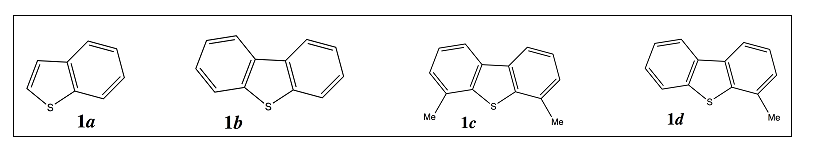
\includegraphics[scale=0.7]{image/P1-F1}
		\caption{Molecular structures studied:  from left to right: benzothiophene \textbf{1\textit{a}}, dibenzothiophene \textbf{1\textit{b}}, 4.6-dimethyldibenzothiophene \textbf{1\textit{c}} and 4-methyldibenzothiophene \textbf{1\textit{d}}}
	\end{figure}
	
	
	\section{Experimental Spectra}
	
	Dibenzothiophene \textbf{1\textit{b}}, 4.6-dimethyldibenzothiophene \textbf{1\textit{c}} and 4-methyldibenzothiophene \textbf{1\textit{d}} were obtained from commercial sources at purity levels of at least 98 per cent and analyzed as received. In some cases, samples were ground manually prior to acquisition of their spectra. 
	
	\bigskip
	
	\subsection{Raman spectra}	

	Raman spectra were obtained using two spectrometers at CanmetENERGY (Devon, Alberta). In one set of experiments, a Renishaw InVia microscope-based system was coupled to a Spectra Physics 125 He-Ne laser, which provided excitation at 633 nm. Several milligrams of each solid were examined with the use of a 50$\times$microscope objective. Spectra were acquired with a spherically focused incident beam; typical resolution was better than 2 cm$^{-1}$. Total accumulation time was 5 min for each spectrum. The second group of experiments was performed with a Bruker IFS 88 FT spectrometer and FRA 106 Raman accessory. Excitation of the FT-Raman spectra was effected with a 1064-nm Nd:YAG laser at power levels between 90 and 260 mW. Ten 32-scan spectra with a resolution of 8 cm$^{-1}$ were averaged for each sample. \\
	
	\subsection{Far-infrared spectra}
	
	\bigskip
	
	PA far-infrared spectra were acquired at a resolution of 6 cm$^{-1}$ using two different Bruker IFS 66v/S Fourier transform infrared (FT-IR) spectrometers. The first instrument, at CanmetENERGY, was operated in both rapid- and step-scan modes. The He-Ne laser modulation frequency was 1.6 kHz for the rapid-scan measurements. Large amplitude phase modulation\cite{michaelian2009far} was employed in the step-scan experiments, with a Signal Recovery lock-in amplifier being utilized for demodulation. The second spectrometer was located at the Canadian Light Source (Saskatoon, Saskatchewan). Rapid-scan spectra were acquired under conditions similar to those just mentioned. A thermal (globar) source was employed with this instrument.\\
	
	Standard MTEC 300 gas-microphone PA accessories were used with both spectrometers; the sample cells were fitted with polyethylene windows. Helium was employed as the carrier gas. Multilayer mylar beam splitters were installed in the interferometers. Spectra were recorded between about 50 and 700 cm$^{-1}$, due to limits imposed by the optical materials. Carbon black powder or an MTEC carbon black reference yielded reference spectra that were used to correct sample spectra for the wavenumber-dependent response of each instrument.\\
	
	\subsection{Mid-infrared spectra}
	
	\bigskip
	
	PA mid-infrared spectra were recorded at a resolution of 6 cm$^{-1}$ using the Bruker IFS 88 spectrometer mentioned above. The laser frequency was either 1.6 or 2.2 kHz. An MTEC 200 PA cell was utilized. Nitrogen was used to purge the spectrometer and as a carrier gas. A KBr window sealed the PA cell, and a Ge/KBr beam splitter was used in the spectrometer. Ten 32-scan spectra were averaged for each sample. Spectra were acquired from about 400 to 4000 cm$^{-1}$. Carbon black powder was used to obtain reference spectra in these experiments.
	
	
	\section{Calculation method for thiophene-type molecules and their dimers}
	
	\subsection{Structural details }
	
	The molecular structures of thiophene-like molecules and their respective dimers were calculated using Density Functional Theory (DFT) with the $\omega$B97X-D exchange-correlation functional and the   6-311++G** basis set, implemented in the Gaussian 09 suite of programs. The $\omega$B97X-D functional developed by Chai \textit{et al}\cite{chai2008systematic} is based on optimized long-range corrected hybrid density functionals, which employ 100\% Hartree-Fock (HF) exchange for long-range electron-electron interaction correction. This method, tested by Salzner \textit{et al}\cite{salzner2011improved} for $\pi$-conjugated oligomers, was also benchmarked successfully for interacting polycondensed aromatic molecules, \cite{spillebout2014discerning} thus proving it overcomes the failure of standard DFT calculation approaches to describe long-distance interactions. The 6-311++G** basis set is of triple-zeta quality for the valence electrons. Among the basis sets tested by Wiberg, \cite{wiberg2004basis} including the Dunning correlation basis sets such as aug-cc-pVTZ and aug-cc-pVQZ, the 6-311++G** basis set gave accurate geometries and frequencies at a relatively small computational cost. The calculations use planar ‘C$_{2}$v symmetry’ for dibenzothiophene, 4.6-dimethyldibenzothiophene, and C$_{s}$ for benzothiophene and 4-dimethyldibenzothiophene. The geometrical parameters of the molecules are benchmarked with experimental data when available.\\
	
	For dimers, as an alternative to the supermolecular treatment, an approach based on symmetry-adapted perturbation theory (SAPT)\cite{jeziorski1994perturbation} which utilizes the description of the interacting monomers in terms of Kohn-Sham (KS) orbitals was used in this work. The DFT-based SAPT approach,\cite{hesselmann2005density} denoted as SAPT-DFT in this work, is exact for all major components of the interaction energy (asymptotically for exchange interactions) in the sense that these energies would be exact if the DFT description of the monomers were exact. It provides accurate results for small dimers such as (C$_{6}$H$_{6}$)$_{2}$ where results for the much more computationally expensive CCSD(T) method are well approximated.\cite{podeszwa2006potential} The SAPT-DFT calculations were performed using the MOLPRO2012 package.\cite{MOLPRO_brief} The PBE0 functional\cite{adamo1999toward} was utilized as a monomer DFT functional in SAPT, using the aug-VTZ basis set. All computational outcomes are reported in the SI.
	
	\section{Resolution of the vibrational Schr\"{o}dinger equation  (RVSE)}
	
	Without any consideration of molecular size, the theoretical process generally developed to solve the Vibrational Schrödinger Equation in the mechanical anharmonic hypothesis requires two restricted steps: the construction of the potential energy surface (PES), and the resolution of the vibrational equation (RVE) in order to obtain the energy levels and consequently the fundamental, overtone and harmonic wavenumbers comprising vibrational spectra. Calculations of the intensities in the electrical anharmonic hypothesis generally complete the analysis of the spectra.\\ 
	
	Owing to the size of the systems studied in this work, we wondered about the precision we could get on PES that include hundreds of thousands of terms. The search for an optimal analytical expression of the PES is an ongoing topic of discussion, even in cases of low-dimensional systems. The skills and experience of some research groups such as that of V. Barone\cite{barone2014fully} show that the PES of large-size systems can be developed by expressing the potential function in a simple way, \textit{i.e.}, a Taylor series expansion using curvilinear displacement coordinates. These series were generally truncated at fourth order. Quadratic, cubic, and quartic force constants were obtained by fitting the electronic energy data generally calculated by DFT methods for various nuclear configurations close to the respective optimized geometry.\\  
	
	Of course, vibrational spectroscopy modeling outcomes are directly dependent on the quality of the potential energy surface (PES) but also depend on the mathematical method used to solve the Schrödinger vibrational equation. In our last work,\cite{garnier2016adaptive} where we focused on the search for a new variational approach to solve this equation, we compiled some methods - direct or indirect, variational or perturbative - that appeared among the most accurate from our point of view. It is generally assumed that variational or VCC (Vibrational Coupled Cluster) approaches take into account the main couplings between the $3N - 6$ vibrational modes of a given system more efficiently than the perturbational approaches. However, the use of such methods is restricted to low-dimension systems (including less than 10 atoms) or highly symmetrical systems. Conversely, vibrational studies of larger systems are now common since the VPT2 approach is implemented in most quantum chemistry codes. To improve the description of perturbations, other combined approaches that attempt to take advantage of both variational and perturbational approaches are utilized. These are known as variation-perturbation methods. Within these approaches, only a few vibrational states $\phi_0^n (q)$ (from tens to thousands constructed from linear combinations of the $3N - 6$ normal modes - see ref\cite{garnier2016adaptive} for notations) strongly coupling the state(s) for which the vibrational characteristics are to be determined are selected by a procedure of interactively enriching the variational space. The energetic correction of all the non-selected states $\varphi_0^n (q)$ is later estimated by perturbation theory. The sum $\textbf{B} = \phi_0^n (q) + \varphi_0^n (q)$ represents the global work basis. Use of these approaches reduces the dimension of the variational problem dramatically\cite{baraille2001calculation,scribano2008iterative} since the dimension of the active space to be diagonalized is, now, under control. At each iteration only a small predetermined number of vibrational states ($\sim$ 100) is needed to obtain the variational space containing the most important couplings. While this procedure converges the active space in a few cycles and leads to matrices (representations of the vibrational Hamiltonian on the basis of the normal modes) of only a few thousand terms for small systems, this approach has yet to converge for systems larger than 20-25 atoms. Here we show that a compromise is always possible in order to reduce the active space dimension that is required to converge the variational problem. Considering that all $3N-6$ vibrational modes of a molecule are not strongly coupled, two ‘truncated’ approaches were developed and tested.\\
	
	Truncation approach n$^{\circ}$1 includes verifying the influence of the truncation of the basis $B$ for studying a mode $x$ (belonging to the T = $3N-6$ ensemble) taking into account, besides the mode being studied, only the X’ = $x$ + $a’$ ($a’$ $\in$ $\mathbb {N}$) lower-frequency and the Y’ = $[3N-6]-y’$ higher-frequency normal modes (where $y’$ stands for the last non-selected mode within the active space) (see Figure \ref{P1-fig2}). Thus, one has a truncated problem dimension equal to T’ = X’ + Y’ $< [3N-6]$. The choice behind this truncation method relies on the fact that large amplitude modes, such as torsion and rotation, are generally coupled to the elongation modes that act on lighter atoms, such as hydrogen. We are interested in these particular modes. Within this truncation, only a few vibrational states ${\phi'}_{0}^{n} (q)$, strongly coupled to the state(s) for which the vibrational characteristics are to be determined, are selected by a procedure that enriches the variational space. The energetic correction of all the non-selected states ${\varphi'}_{0}^{n} (q)$ is then estimated by perturbation theory. The sum $\textbf{B’} = {\phi'}_{0}^{n} (q) + {\varphi'}_{0}^{n} (q)$ represents the new reduced global work basis.\\
	
	Truncation approach n$^{\circ}$2 was used to verify a hypothesis normally assumed to be true - that every $x$ state is \textit{a priori} more strongly coupled with its closest energetic neighbors. To do so, we have prepared an alternate selection criterion. Concerning the selection of the lower-frequency modes, we state a new criterion based on the selection of X'': in order to study a vibrational state $x$, one must select $2x"$ normal modes within the basis ($x"$ being a positive integer) (see Figure \ref{P1-fig2}). The selected $2x"$ normal modes within the truncated basis are exactly those that are energetically as close as possible to $x$. This basis has X''=1+$2x"$ lower-frequency and Y’’=Y’ higher-frequency states. The final dimension of this new basis is T''=X''+Y''. If $x"$ equals zero, this is the same as studying the influence of high-energy stretching modes on $x$. This new procedure generates a new working basis denoted $\textbf{B''}$.
	
	\begin{figure}[H]
		\begin{center}
			
			\begin{tikzpicture}[thick, scale=.5, >=stealth]
			\draw[black] (1, 0) -- (24, 0);
			\draw[line width=3pt, red] (1, 0) -- (9, 0) (18, 0) -- (24, 0);
			\foreach \x in {1, 2, ..., 24} {
				\draw (\x, -.2) -- (\x, .2);
			}
			\node at (6, .5) {$x$};
			\node at (17, .5) {$y$};
			\node at (1, .5) {$1$};
			\node[right] at (24, .5) {$3N-6$};
			\draw[<->] (6, -1) -- (9, -1) node[below, pos=.5] {$a'$};
			\draw[<->] (1, -.5) -- (9, -.5) node[below, pos=.5] {X'};
			\draw[<->] (18, -.5) -- (24, -.5) node[below, pos=.5] {Y'};
			\end{tikzpicture}
			
			\begin{tikzpicture}[thick, scale=.5, >=stealth]
			\draw[black] (1, 0) -- (24, 0);
			\draw[line width=3pt, red] (4, 0) -- (8, 0) (18, 0) -- (24, 0);
			\foreach \x in {1, 2, ..., 24} {
				\draw (\x, -.2) -- (\x, .2);
			}
			\node at (6, .5) {$x$};
			\node at (17, .5) {$y$};
			\node at (1, .5) {$1$};
			\node[right] at (24, .5) {$3N-6$};
			\draw[<->] (4, -1.65) -- (6, -1.65) node[below, pos=.5] {$x''$};
			\draw[<->] (6, -1.65) -- (8, -1.65) node[below, pos=.5] {$x''$};
			\draw[<->] (18, -.5) -- (24, -.5) node[below, pos=.5] {Y''};
			\draw[<->] (4, -.5) -- (8, -.5) node[below, pos=.5] {X''};
			\end{tikzpicture}  
			
		\end{center}
		\caption{Selection of normal modes which are stored in the expression of the PES  : methodologies applied to realize the !truncation of the vibrational basis a) truncation n$^{\circ}$1 T’=X’+Y’; b) truncation n$^{\circ}$2 T’’=X’’+Y’’} \label{P1-fig2}
	\end{figure}
	
	\section{Results and Discussion}
	
	\subsection{Monomers}
	
	Benzothiophene (N=15) and dibenzothiophene (N=21) were chosen to test basis truncation. For each of these systems, a fully converged calculation of the variation-perturbation type was performed. The ensembles of the results obtained using the two truncated bases for the first twelve modes for benzothiophene are reported in Figures 3 (truncation n$^{\circ}$1) and 4 (truncation n$^{\circ}$2).  Of these twelve modes, modes 1, 2, 4, 5, 8, 10 and 12 occur in the C$_{s}$ plane whereas modes 3, 6, 7 and 9 are out of the C$_{s}$ plane. Since the outcomes of the test for the first nine modes of dibenzothiophene are comparable, they are provided in the supporting information as Figure S2.\\
	
	For truncation n$^{\circ}$1, the main results are reported here in Figures 3a - 3l. The information reported in these graphs represents the difference obtained on the calculation of a target vibration frequency in the reduced basis $\textbf{B’}$ from the result that would be obtained using the same variation–perturbation method with the full basis $\textbf{B}$. For example, the analysis of the target mode 1 (X’=1, Figure 3a) shows that the presence of only the higher-frequency $\omega_{CH}$ stretching modes suffices to describe the vibrational problem concerning this mode. This observation accords well with the hypothesis that only the large amplitude modes are strongly coupled with the elongation ones involving lighter atoms. The analysis of the other out-of-plane C$_{s}$ deformation modes (2, 4, 5 and 8) leads to similar conclusions. The results of the calculation on mode 2 are closer to those obtained for mode 1, which seems logical since these two vibrational modes are \textit{de facto} similar. Concerning modes 4 and 5, regardless of the number of selected states within the basis created from the X’ criterion, one can note the need to work with at least 13 modes on the Y’ basis in order to be as close as possible to the reference calculation. On the other hand, one observes that it is not necessary to take into account all the lower-frequency modes within the basis for the calculation to converge. This will be confirmed shortly by the analysis of the second truncation. Another striking observation also emerges from this analysis: if it is desirable to introduce some of the wagging, scissoring and stretching modes in the basis, the calculation will converge satisfactorily only if all of these modes are introduced at the beginning. Concerning mode 8, it can be noted that no truncation seems capable of leading to an acceptable convergence.\\
	
	We have added the results for modes 10 and 12 although they do not belong to the same low-frequency category considered in this study. These two modes lie at the interface between the low-frequency and the other modes. The main conclusion one can derive from them is that taking into account only the low frequency and $\omega_{CH}$ modes in the basis no longer suffices for convergence of the calculations. These conclusions are generalized beyond mode 12.\\
	
	The modes taking place in the plane of the molecule, \textit{i.e.} modes 3, 6, 7, 9 and 11, again corroborate our hypothesis; particularly for low-frequency mode 3. In addition, the $x’$ modes that are close to mode 3 seem to have no effect on the quality of the converged result. The descriptions of modes 6 and 7 show again that the results are not greatly dependent on the basis truncation unless all the $\omega_{CH}$ modes were previously selected. Analyzing the results for modes 9 and 11 leads to the same conclusion, except that a strong truncation of Y’ would cause a much more important deviation of the results from those observed for modes 3, 6 and 7.\\
	
	The analysis of the results concerning the second truncation allows one to confirm even more the observations just presented. Only the results obtained for the modes 4, 5, 6 and 8 are reported here. Representations of these results were added as a second layer to those obtained beforehand (Figure 4a-d insets); the two situations are connected by a series of points they share in common, \textit{i.e.} when $a’$=$x"$. The main information we can derive from these studies is that no low-frequency mode requires its closest neighbors to ensure a good convergence of the results. Every argument indicates that these modes are only coupled to those involving $\omega_{CH}$ stretching. Only modes 4 and 5 seem to slightly depend on each other.\\
	
	\begin{figure}[H]
		\begin{center}
			\begin{tabular}{c c c}
				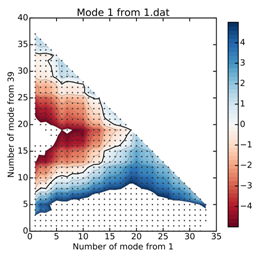
\includegraphics{image/P1-F311} & 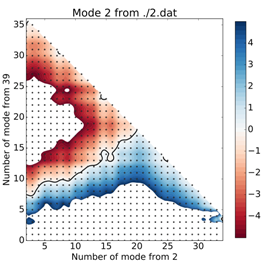
\includegraphics{image/P1-F312} &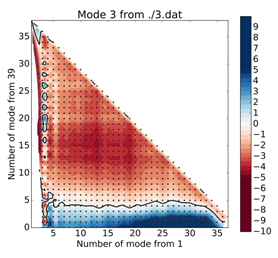
\includegraphics{image/P1-F313} \\
				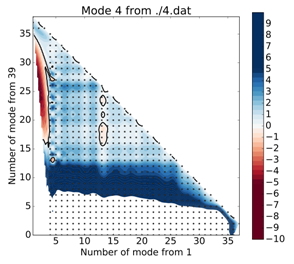
\includegraphics{image/P1-F321} & 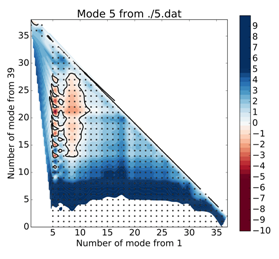
\includegraphics{image/P1-F322} & 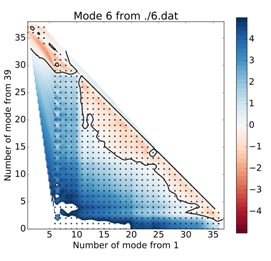
\includegraphics{image/P1-F323} \\
				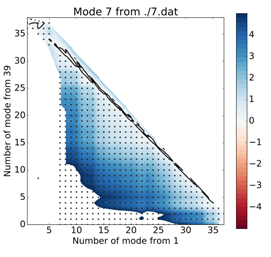
\includegraphics{image/P1-F331} & 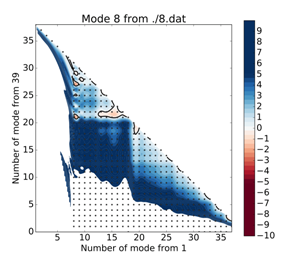
\includegraphics{image/P1-F332} & 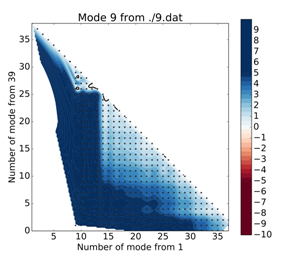
\includegraphics{image/P1-F333} \\
				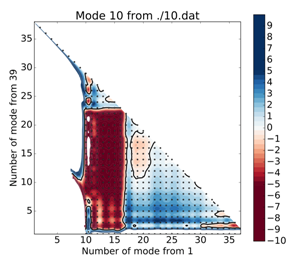
\includegraphics{image/P1-F341} & 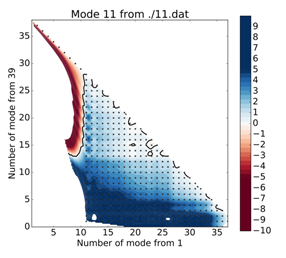
\includegraphics{image/P1-F342} & 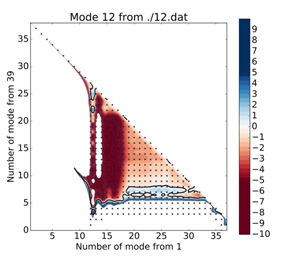
\includegraphics{image/P1-F343}\\   \label{P1-F3}
			\end{tabular}
		\end{center}
		\caption[Ensemble of results obtained using truncation n$^{\circ}$1 for the first twelve modes of a benzothiophene molecule]{Ensemble of results obtained using truncation n$^{\circ}$1 for the first twelve modes of a benzothiophene molecule. Mode 1: Figure 3a; Mode 2: Figure 3b … Mode 12: Figure 3l.
			In the $z$ axis are reported the values of the difference obtained on calculating a frequency without any truncation and the same frequency calculated in base $\textbf{B’}$ (T’=X’+Y’; X’ axis $x$; Y’ axis $y$; in accordance with the notation used in Figure \ref{P1-fig2}).}
	\end{figure}
	
	In summary, variational-perturbational studies using a truncated basis taking into account the closest neighbors of the low-frequency modes seems not to be an essential requirement for describing their vibrational properties as opposed to their coupling with the high-frequency stretching $\omega_{CH}$ modes. Finally, variational-pertubational studies using a truncated basis were performed for systems \textbf{1\textit{a}} (benzothiophene), \textbf{1\textit{b}} (dibenzothiophene), \textbf{1\textit{c}} (4,6-dimethyldibenzothiophene) and \textbf{1\textit{d}} (4-methyldibenzothiophene). The same was done for their dimers and compared against experimental results obtained by IR and Raman spectroscopy.
	
	
	\begin{figure}[H]
		\begin{center}
			\begin{tabular}{c c}
				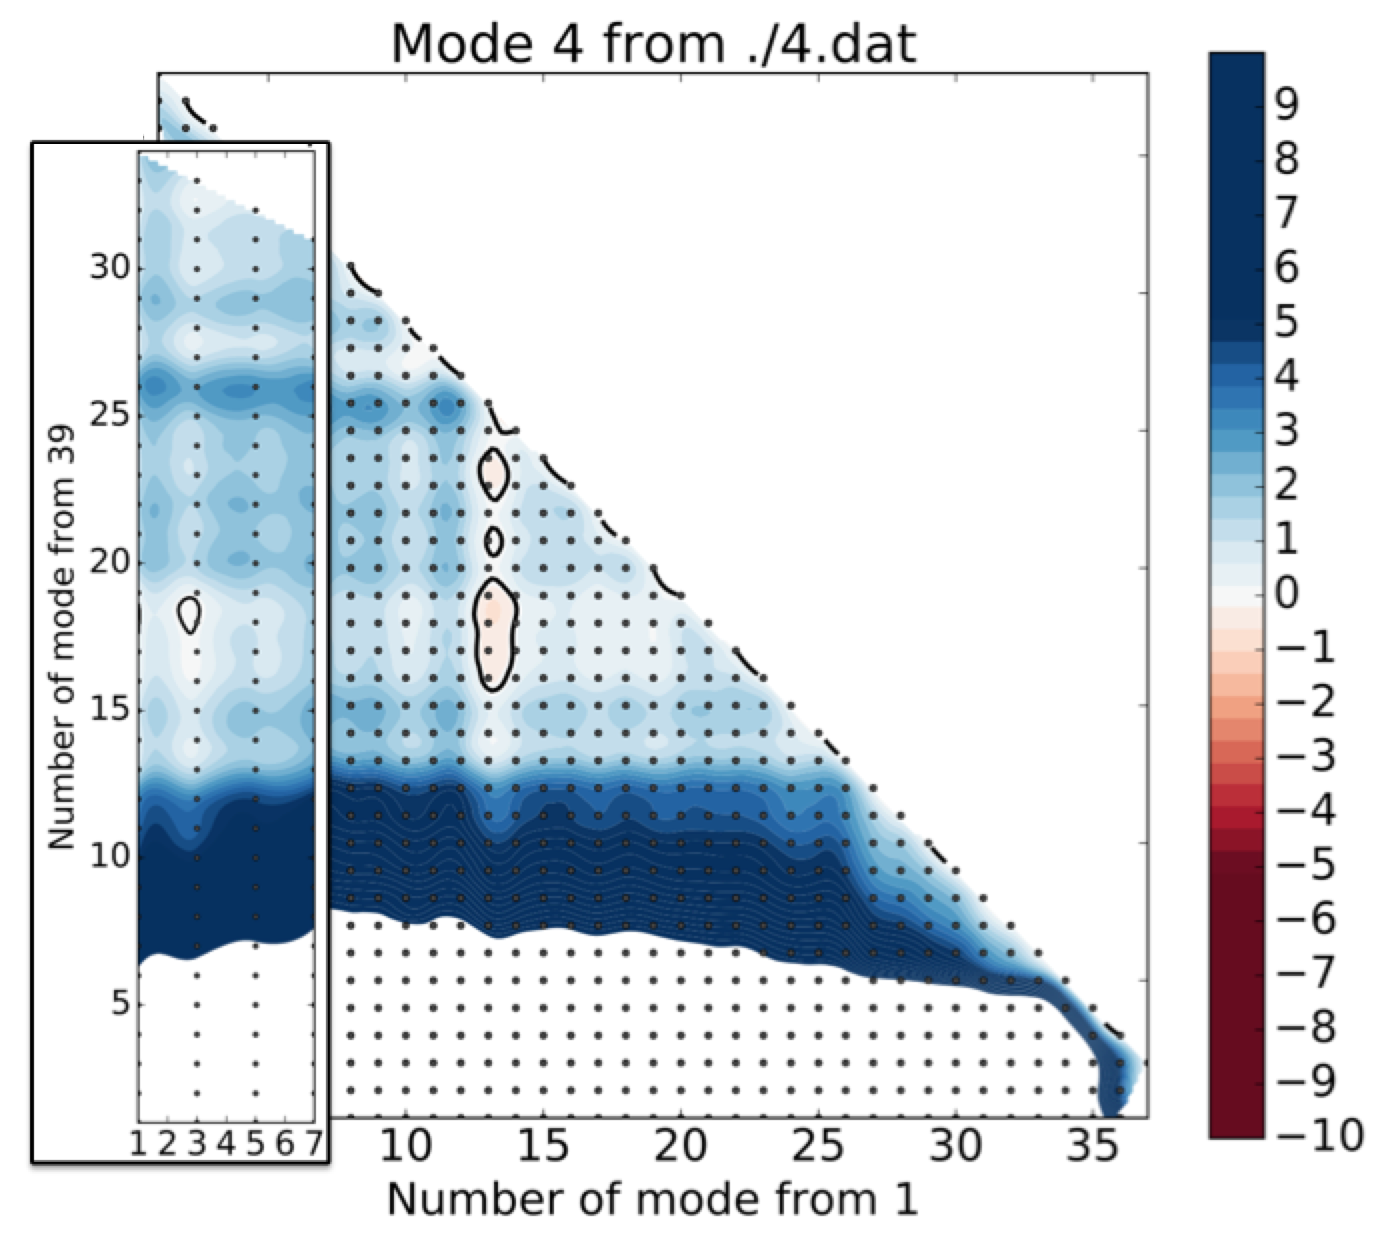
\includegraphics[scale=0.2]{image/P1-41} & 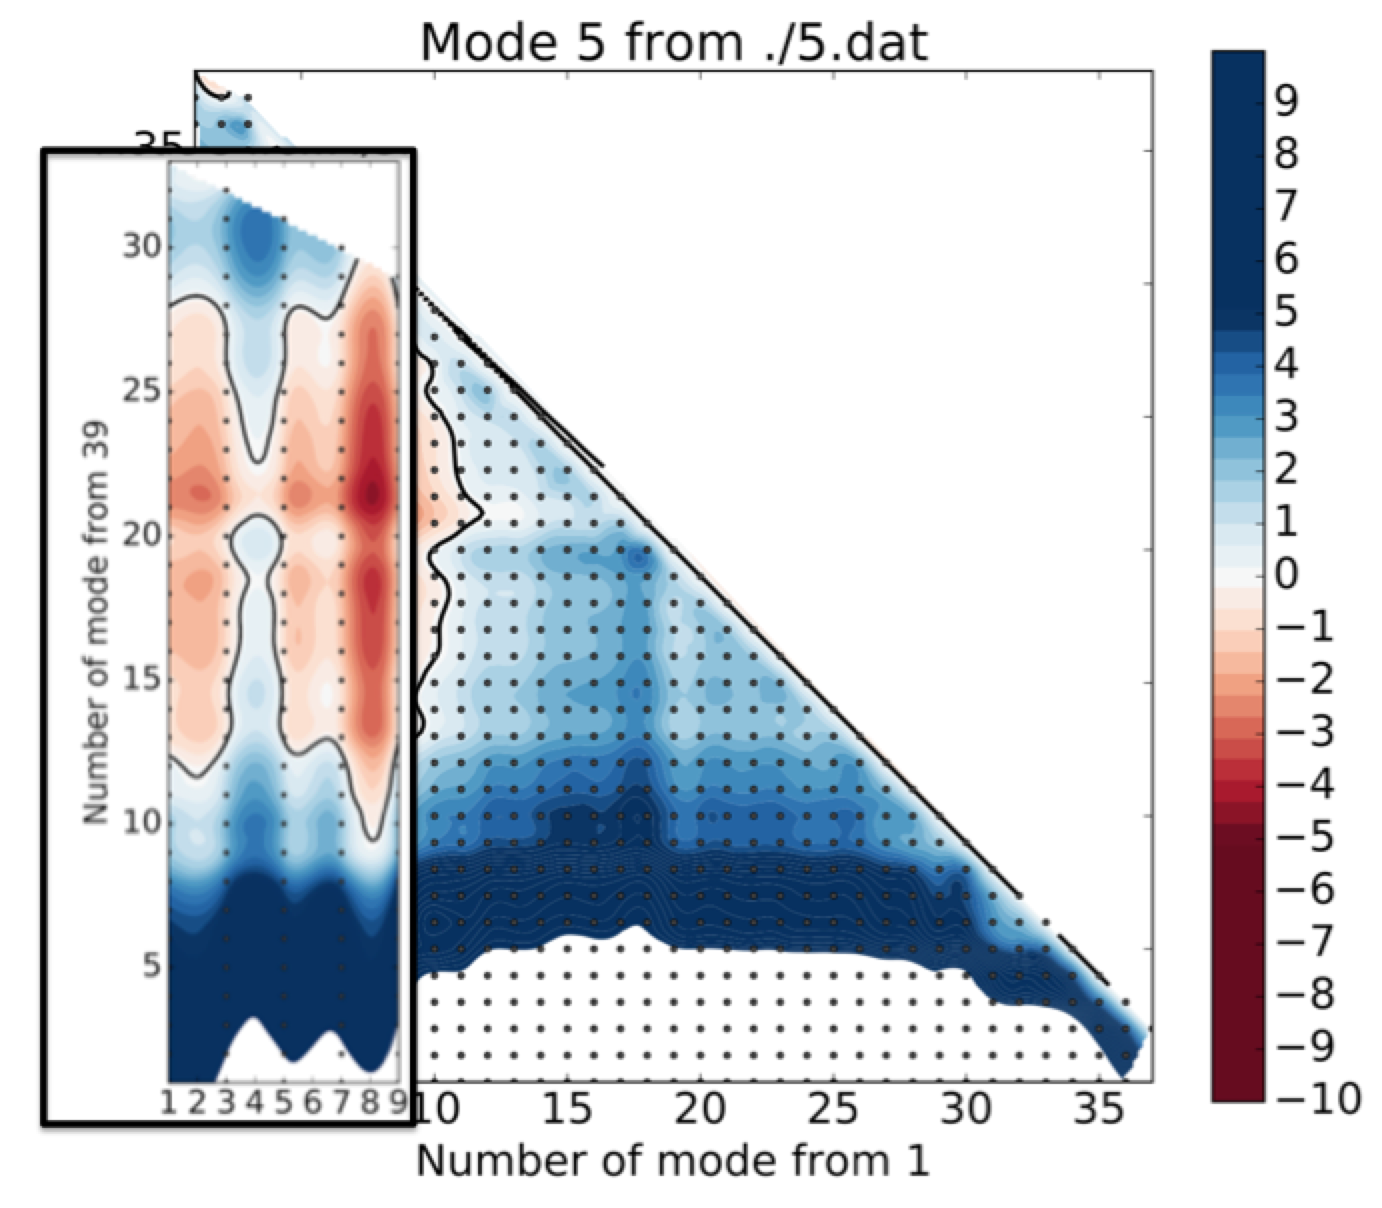
\includegraphics[scale=0.2]{image/P1-42}\\
				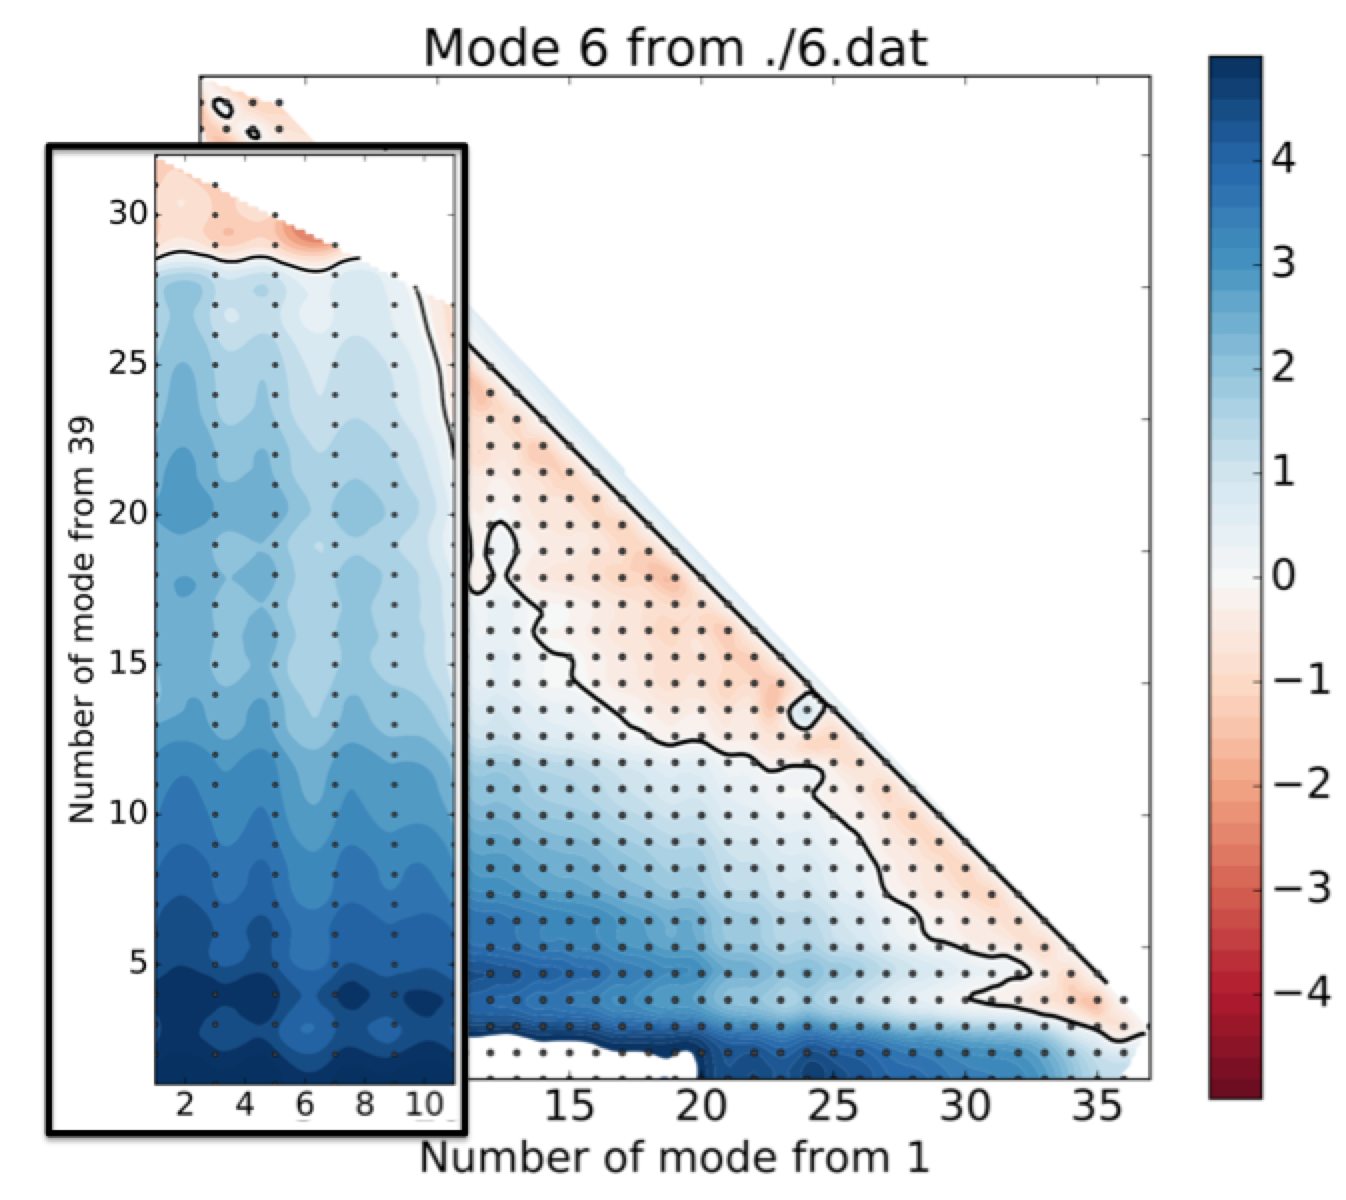
\includegraphics[scale=0.2]{image/P1-43} & 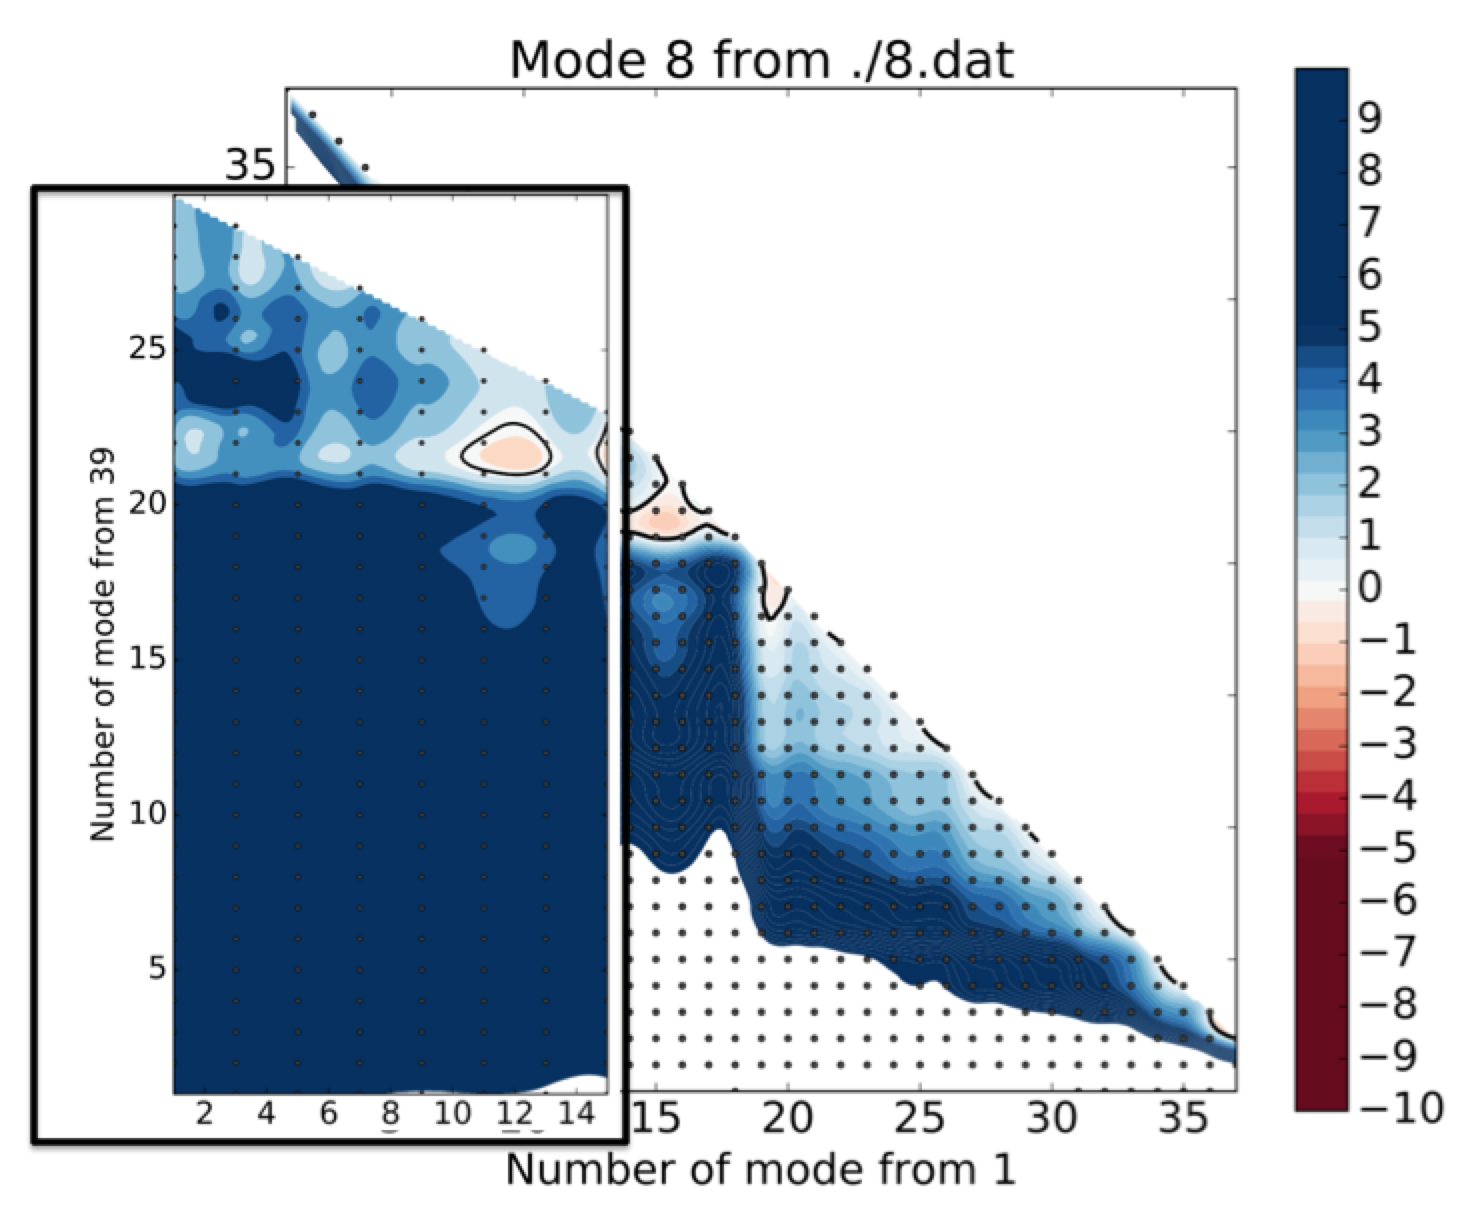
\includegraphics[scale=0.2]{image/P1-44}\\
			\end{tabular}
		\end{center}
		\caption[Ensemble of results using the truncation n$^{\circ}$2 for the first twelve vibration modes of a benzothiophene molecule]{Ensemble of results using the truncation n$^{\circ}$2 for the first twelve vibration modes of a benzothiophene molecule. Mode 4: Figure 4a; Mode 5: Figure 4b; Mode 6: Figure 4c;  Mode 8: Figure 4d.
			In the z axis are reported the values of the difference obtained on calculating a frequency without any truncation and the same frequency calculated in base $\textbf{B’’}$ (T’’=X’’+Y’’; X’’ axis $x$; Y’’=Y’ axis $y$; in accordance with the notation used in Figure \ref{P1-fig2}).}
	\end{figure}
	
	
	PA infrared and Raman spectra of \textbf{1\textit{b}} (dibenzothiophene), \textbf{1\textit{c}} (4,6-dimethyldibenzothiophene) and \textbf{1\textit{d}} (4-methyldibenzothiophene) were interpreted in light of the quantum chemistry calculations. Data for \textbf{1\textit{a}} (benzothiophene) were taken from the literature. The low-wavenumber and “fingerprint” regions (comprising, together, the 20–2000 cm$^{-1}$ range) were studied in detail in these investigations. In addition to the predicted infrared-active bands, the PA spectra of these hydrocarbons display many features due to overtones and combinations. Moreover, numerous Raman-active (gerade) vibrations also give rise to bands in the PA spectra, which thus convey considerable information regarding the structures of these compounds.\\
	
	
	\textit{Low wavenumber region (~100–700 cm$^{-1}$)}: both Raman and infrared spectroscopy results for \textbf{1\textit{a}} benzothiophene and \textbf{1\textit{b}} dibenzothiophene are reported in Tables 1 and 2. Raman and PA infrared results for \textbf{1\textit{c}} 4,6-dimethyldibenzothiophene and \textbf{1\textit{d}} 4-methyldibenzothiophene are given in Tables S8 and S9.\\
	
	
	For the benzothiophene molecule, the reported Raman spectrum has no significant features in this region. The IR spectrum is dominated by three intense bands at 471, 560 and 690 cm$^{-1}$ which are characteristic of wagging modes. Two other combination modes are IR-active. They are not easily detected since they have very low intensity and also due to the fact that the $\nu_{2}+ \nu_{5}$ mode has a signature very close to that of the active fundamental mode $\nu_{9}$. The analysis of the active modes of the dibenzothiophene molecule (Figure 5) shows that two of the three most intense wagging modes (\textit{obs} 497 and 704 cm$^{-1}$), which are, incidentally, characteristic of benzothiophene, can be clearly distinguished and do not allow one to easily separate the molecules from each other. However, one should note that a characteristic shift towards higher frequencies is found for these two modes of the dibenzothiophene system. Also note, in comparison to benzothiophene, an extinction (near 560 cm$^{-1}$) of the wagging signature because of symmetry induction and a new intense characteristic vibration located around 615 cm$^{-1}$. Moreover, the IR spectrum of this molecule for the region between 100 and 450 cm$^{-1}$ is more complex and richer in spectral features. As a matter of fact, other stronger and medium intensity modes signify the presence of the second benzyl moiety within the dibenzothiophene molecule. This observation agrees very well with our calculations. The analysis of the eigenfunctions generated by the variational-perturbational process shows that these modes are mainly developed on the basis of vibrational states that are characteristic of torsion ($\nu_{3}$(a$_{1}$) 213 cm$^{-1}$; \textit{calc} 217 cm$^{-1}$), breathing ($\nu_{4}$(b$_{1}$) 228 cm$^{-1}$; \textit{calc} 221 cm$^{-1}$) and ($\nu_{6}$(a$_{1}$) 404 cm$^{-1}$; \textit{calc} 416 cm$^{-1}$) and wagging ($\nu_{8}$(b$_{1}$) 425 cm$^{-1}$; \textit{calc} 433 cm$^{-1}$) combination modes of the benzenic rings. \\
	
	The Raman signature of the dibenzothiophene molecule is also more complex than that of benzothiophène. In the present context, this fact introduces only limited information since most of the active Raman modes are already the most intense and characteristic of the IR spectrum. All the other active modes have very low intensities which are again in agreement with our calculations. It is worth noting the confirmation provided by the Raman results concerning the shoulder observed in the IR spectrum around 419 cm$^{-1}$. 
	Similarly to the benzothiophene molecule two combination modes are foreseen by the calculations that can be, mainly for the $\nu_{2}+\nu_{8}$ mode, reasonably assigned experimentally.\\
	
	In addition to some frequency shifts, the spectra of both 4-methyldibenzothiophene and 4,6-dimethyldibenzothiophene exhibit important changes in the intensities of the vibrations in the 100 - 500 cm$^{-1}$ region as compared with the spectrum of dibenzothiophene. The clearest change occurs in the 400-460 cm$^{-1}$ region; the presence of substituents induces a significant change in intensity, ranging from very intense modes down to nearly zero (notably for the $\nu_{10}$ mode of 4-methyldibenzothiophene). These differences are even more pronounced in the Raman spectra. Whilst the presence of a single methyl group does not significantly change the Raman signature of the dibenzothiophene molecule, a second substitution in the 4,6 position does so very pronouncedly. The main change concerns the most characteristic mode of the di-substitution found at 598 cm$^{-1}$, which represents an in-phase breathing mode of the three rings.
	
	\begin{table}[H]
		\begin{center}
			\caption[Low wavenumber Raman and infrared spectra of benzothiophene]{Low wavenumber Raman and infrared spectra of benzothiophene (\textit{C$_s$ symmetry})}
			\begin{threeparttable}[b]
				\begin{tabular}{c c c c c}
					\toprule
					\multicolumn{2}{p{5cm}}{\centering \textbf{Observed$^{b}$}} & \multicolumn{3}{p{10cm}}{\centering \textbf{Calculation}} \\
					Raman & Infrared & Mode & $\omega^{a,c}$ & $\nu^{d}$ \\
					\midrule
					&  &   &    &   \\
					192 vw & 192 vw & $\nu_{1}$ (A") & 196 (0.22) [0.27] & 194 (0.20)\\
					& 198-212 w & $\nu_{2}$ (A") & 204 (4.11) [0.12] & 199 (2.97) \\
					340 vw & 340 vw & $\nu_{3}$ (A') & 351 (2.82) [2.11] & 345 (2.08) \\
					387 vw &   & $\nu_{1} + \nu_{2}$ &  & 391 (0.03) \\
					& 405-411 vw & $\nu_{4}$ (A") & 427 (3.45) [0.77] & 414 (2.50)\\
					& 471 m & $\nu_{5}$ (A") & 482 (5.88) [0.53] & 478 (6.02) \\
					491 vw & 491-497 vw & $\nu_{6}$ (A') & 500 (0.30) [10.64] & 494 (0.29) \\
					526 vw &  & $\nu_{7}$ (A') & 538 (0.25) [6.54] & 533 (0.36) \\
					& 558-564 m & $\nu_{8}$ (A") & 578 (5.88) [0.70] & 563 (5.24)\\
					& 669 vw & $\nu_{9}$ (A') & 683 (2.32) [1.47] & 675 (1.70)\\
					&  & $\nu_{2} + \nu_{5}$ &  & 679 (0.10) \\
					& 690 s & $\nu_{10}$ (A") & 710 (34.70) [0.23] & 692 (28.22)\\
					\bottomrule 
				\end{tabular}
				
				\begin{tablenotes}
					\item[a] Infrared intensities (in parentheses) in km/mol and Raman intensities [in brackets] in A$^{4}$/AMU.
					\item[b] Experimental data. Relative intensities: vw = very weak, w = weak, m = medium, s = strong, vs = very strong, sh = shoulder.
					\item[c] Unscaled DFT frequencies calculated using $\omega$B97X-D/6-311++G**.
					\item[d] Anharmonic $\omega$B97X-D/6-311++G** calculation using the A-VCI algorithm\cite{garnier2016adaptive}.
				\end{tablenotes}
			\end{threeparttable}
		\end{center}
	\end{table}
	
	
	\begin{figure}[H]
		\centering
		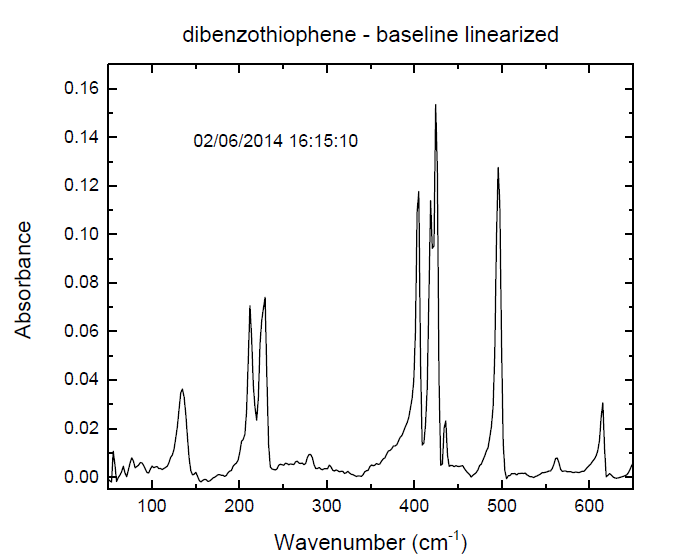
\includegraphics[scale=0.53]{image/Spectra-diben}  \label{P1-spectradiben}
		\caption{Far-infrared PA spectra of dibenzothiophene}
	\end{figure}
	
	
	
	\begin{table}[H]
		\begin{center}
			\caption[Low wavenumber Raman and infrared spectra of dibenzothiophene]{Low wavenumber Raman and infrared spectra of dibenzothiophene (\textit{C$_{2v}$ symmetry})}
			\begin{threeparttable}[b]
				\begin{tabular}{c c c c c}
					\toprule
					\multicolumn{2}{p{5cm}}{\centering \textbf{Observed$^{b}$}} & \multicolumn{3}{p{10cm}}{\centering \textbf{Calculation}} \\
					Raman & Infrared & Mode & $\omega^{a,c}$ & $\nu^{d}$ \\
					\midrule
					&  &   &    &   \\
					138 w & 135 m & $\nu_{1}$ (b$_{1}$) & 102 (1.54) [0.28] & 101 (0.66) \\
					171 w &  & $\nu_{2}$ (a$_{2}$) & 135 (0.00) [0.07] & 133 (0.01)\\
					217 m & 213 m & $\nu_{3}$ (a$_{1}$) & 217 (0.85) [1.25] & 208 (1.23) \\
					232 w & 228 m & $\nu_{4}$ (b$_{1}$) & 221 (1.46) [1.03] & 223 (1.42) \\
					& 269 vw &  &  &  \\
					282 w & 282 vw & $\nu_{5}$ (a$_{2}$) & 279 (0.00) [2.90] & 274 (0.00)\\
					287 sh & &  &  & \\
					410 s & 404 s & $\nu_{6}$ (a$_{1}$) & 416 (2.83) [13.05] & 409 (2.80)\\
					& 419 sh & $\nu_{7}$ (b$_{2}$) & 428 (0.14) [2.72] & 425 (0.15) \\
					419 m & 425 s & $\nu_{8}$ (b$_{1}$) & 433 (7.15) [0.01] & 425 (5.06) \\
					437 vw & 436 w & $\nu_{9}$ (a$_{2}$) & 444 (0.00) [0.06] & 438 (0.00) \\
					& 460 vw  &  &   & \\
					496 w & 497 s & $\nu_{10}$ ($_{1}$) & 505 (0.28) [4.76] & 499 (0.22) \\
					&  & $\nu_{12}$ (b$_{2}$) & 511 (1.23) [4.67] & 497 (1.48)\\
					504 vw & 512 w & $\nu_{11}$ (b$_{1}$) & 510 (2.74) [0.03] & 504 (1.18) \\
					& 565 w & $\nu_{2} + \nu_{8}$ (b$_{2}$) &   & 562 (0.12)\\
					&   &   $\nu_{13}$ (a$_{2}$) & 580 (0.00) [0.24] & 568 (0.00) \\
					& 615 m & $\nu_{14}$ (b$_{2}$) & 635 (5.09) [0.04] & 627 (4.62)\\
					& 667 w & $\nu_{17}$ (b$_{1}$) & 730 (0.82) [0.00] & 666 (0.15)\\
					&   &  $\nu_{3} + \nu_{10}$ (b$_{2}$) &  & 675 (0.01)\\
					703 s &704 vs &  $\nu_{15}$ (b$_{2}$) & 724 (6.53) [5.58] & 713 (6.43) \\
					\bottomrule 
				\end{tabular}
				
				\begin{tablenotes}
					\item[a] Infrared intensities (in parentheses) in km/mol and Raman intensities [in brackets] in A$^{4}$/AMU .
					\item[b] Experimental data from this work and ref\cite{bree1971vibrations}. Relative intensities: vw = very weak, w = weak, m = medium, s = strong, vs = very strong, sh = shoulder.
					\item[c] Unscaled DFT frequencies calculated using $\omega$B97X-D/6-311++G**.
					\item[d] Anharmonic $\omega$B97X-D/6-311++G** calculation using the A-VCI algorithm\cite{garnier2016adaptive}.
				\end{tablenotes}
			\end{threeparttable}
		\end{center}
	\end{table}
	
	
	
	
	
	\section*{Dimers}
	
	Characterization of the spectral signatures of “isolated” thiophene molecules constitutes the first part of this study. The second aim of this work lays in the identification and characterization of the IR and Raman signatures of the vibration modes at very low wavenumbers which are characteristics of associated systems such as dimers. In order to foresee and identify the spectral signatures typical of these interactions, we have first identified all the stable forms of benzothiophene (and its derivatives) dimers, \textit{i.e.}, \textbf{2\textit{a}} d-benzothiophene, \textbf{2\textit{b}} d-dibenzothiophene, \textbf{2\textit{c}} d-4-methyldibenzothiophene and \textbf{2\textit{d}} d-4,6-dimethylbenzothiophene. Among all the possible dimer configurations, eight types of benzothiophene dimers have been calculated; these are represented in Figure 6. In all tables and figures, the letter \textit{d} means dimer. The geometrical parameters are summarized in SI.  Our interest lies in $\pi$-stacking interactions, hence we have considered the molecules placed such that $\pi-\pi$ stacking interactions are favored.
	
	Although $\pi-\pi$ stacking interactions have been proven to be predominant, electrostatic interactions also induce specific configurations \cite{liu2014adjusting}. In order to validate the calculation method used, additional calculations using SAPT-DFT have been performed and geometrical parameters as well as interaction energies calculated with the two methods are compared. The energies for the different configurations of the benzothiophene molecule are reported in Table 3. The energies for all the configuration for the three other systems (\textbf{2\textit{b}}-\textbf{2\textit{c}}), the graphical representations and optimized structures can be found in the SI.
	
	
	\begin{figure}[H]
		\centering
		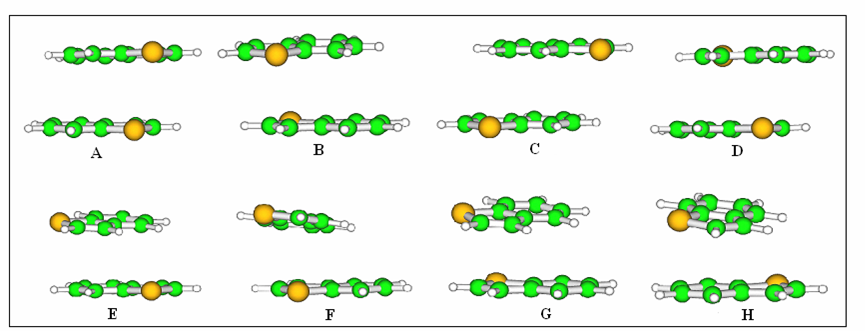
\includegraphics[scale=0.88]{image/P1-F6} \label{P1-F6}
		\caption{Configurations of benzothiophene dimers optimized at the $\omega$B97X-D/6-311++G** level of theory.}
	\end{figure}
	
	\begin{figure}[H]
		\centering
		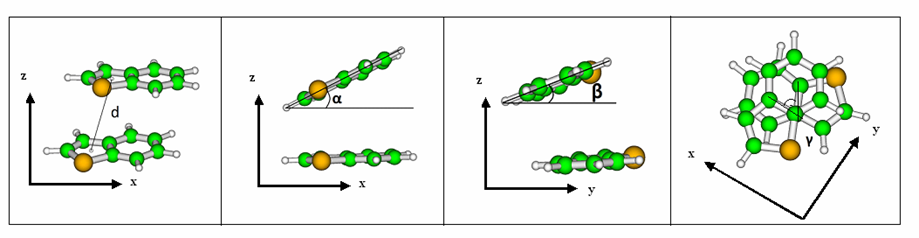
\includegraphics[scale=0.88]{image/P1-F7}  \label{P1-F7}
		\caption{Structural parameters of benzothiophene dimers}
	\end{figure}
	
	\noindent d = Intermolecular distance between thiophene rings center of benzothiophene dimers.\\
	$\alpha$ = Angle between the molecules inside $x$, $z$ plane. \\
	$\beta$ = Angle between the molecules inside $y$, $z$ plane.\\
	$\gamma$ = Angle of rotation in $z$ axis.\\
	
	
	\begin{table}[H]
		\caption[Interaction energies of benzothiophene dimers]{(a) Interaction energies of benzothiophene dimers (kcal/mol) in 8 different configurations using $\omega$B97X-D/6-311++G**, and compared with other methods. (b) Intermolecular distance between thiophene rings center of benzothiophene dimers (Å) (c) Angle between ring planes of benzothiophene dimers ($^{\circ}$) according to Figure 6. (d) Angle between ring planes of benzothiophene dimers ($^{\circ}$) according to Figure 6. Energies taking into account zero-point energy (ZPE) and Basis Set Superposition Error (BSSE) corrections.}
		\begin{center}
			\begin{threeparttable}[b]
				\resizebox{17cm}{!}{
					\begin{tabular}{c c c c c c c c c c}
						(a) &  &   &   &   &  &  &  &  & \\
						\toprule
						&	&  \textbf{A} & \textbf{B} & \textbf{C} & \textbf{D} & \textbf{E} & \textbf{F} & \textbf{G}& \textbf{H} \\
						\midrule
						\multicolumn{2}{p{5cm}}{\centering \small{$\omega$B97x-D/} \\ \small{6-311++G**}}  & -6.41 &  -7.05 & -6.83 & -7.11 & -7.23 & -7.01 & -7.02 & -7.00 \\
						\multicolumn{2}{p{5cm}}{\centering \small{DFT-SAPT(PBE0)} \\ \small{aug-cc pVTZ}}  & -5.33 & -5.73 & -5.56 & -5.95 & -5.83 & -5.87 & -5.72 & -5.63 \\
						\multicolumn{2}{p{5cm}}{\centering \small{B971/} \\ \small{6-31+G(d,p)-DCP$^{a}$}}  & -5.46 & -5.80 & -5.72 & -5.68 & -5.13 & -5.40 & -5.10 & -4.76 \\
						\bottomrule 
						\\
						\\
						\raggedleft (b)&  & & &   &  &  &  &   & \\
						\toprule
						& & \textbf{A} & \textbf{B} & \textbf{C} & \textbf{D} & \textbf{E} & \textbf{F} & \textbf{G}& \textbf{H} \\
						\midrule
						\multicolumn{2}{p{5cm}}{\centering \small{$\omega$B97x-D/} \\ \small{6-311++G**}}  & 3.94 & 3.81 & 5.28 & 3.72 & 4.49 & 3.56 & 3.74 & 4.37 \\
						\multicolumn{2}{p{5cm}}{\centering \small{DFT-SAPT(PBE0)} \\ \small{aug-cc pVTZ}}  & 3.98 & 3.80 & 5.16 & 3.75 & 4.53 & 3.65 & 3.70 & 4.30\\
						\multicolumn{2}{p{5cm}}{\centering \small{B971/} \\ \small{6-31+G(d,p)-DCP$^{a}$}} & 3.99 & 3.84 & 4.65 & 3.83 & 5.03 & 3.66 & 3.75 & 3.70\\
						\bottomrule
						\\
						\\
						(c) &   &   &   &  &  & &   &   & \\
						\toprule
						& &  \textbf{A} & \textbf{B} & \textbf{C} & \textbf{D} & \textbf{E} &  \textbf{F} & \textbf{G}& \textbf{H}  \\
						\midrule
						\multicolumn{1}{p{3cm}}{\centering \textbf{$\alpha$}} & &2.94 &1.73 &1.06 &0.44 &2.23  &4.38   &2.05  &6.37 \\
						\multicolumn{1}{p{3cm}}{\centering \textbf{$\beta$}}  & &3.59 &4.23 &3.14 &0.51 &5.07  &13.28  &9.03  &5.64 \\
						\multicolumn{1}{p{3cm}}{\centering \textbf{$\gamma$}} & &     &     &     &     &68.92 &100.06 &51.71 &77.25\\
						\bottomrule
						\\
						\\
						(d) &   &   &   &  &  & &   &   & \\
						\toprule
						& & \textbf{A} & \textbf{B} & \textbf{C} & \textbf{D} & \textbf{E}  &  \textbf{F} & \textbf{G}& \textbf{H} \\
						\midrule
						\multicolumn{1}{p{4cm}}{\centering \textbf{$\alpha$}} & &2.11 & 1.60 & 2.36 &1.49 & 3.50 & 2.66 & 11.90 & 7.97\\
						\multicolumn{1}{p{4cm}}{\centering \textbf{$\beta$}}& &4.00 & 3.67 &2.33 &2.00 &12.76 & 2.37 & 15.79 & 5.82\\
						\multicolumn{1}{p{4cm}}{\centering \textbf{$\gamma$}} & & &  &  &  &  108.52 & 105.27 & 107.62 & 51.44\\
						\bottomrule
					\end{tabular}}
					
					\begin{tablenotes}
						\item[a] ref\cite{mackie2010importance}
					\end{tablenotes}
				\end{threeparttable}
			\end{center}
			\label{P1-table3}
		\end{table}
		
		
		Eight conformations were highlighted for the benzothiophene dimer species. Benchmark energy calculations were performed using the DFT-SAPT(PBE0)/aug-cc pvtz level of theory. The $\omega$B97X-D/ 6-311++G** calculations, from which the vibrational calculations were performed taking into account both electrical and mechanical anharmonicities, lead to the same conclusions concerning the stability of these eight conformers (average deviation on the order of 1.25 kcal/mol). Regardless of the theory level that is employed, the two most stable conformations are \textbf{D} and \textbf{E}. In these conformations, the sulfur atoms are opposed to each other. This is also the case for the majority of the other systems studied in this work. The analysis of the energetic contributions linked to the intermolecular association phenomena is reported in Table 4.\\
		
		Before commenting on the results obtained by these contributions, one should recall the basis of the SAPT method used here. The van der Waals interactions, responsible for the cohesion of the dimers reported in this work, are clearly distinct to other types of long-range interactions. In the intermediate region that includes the minimum, it is very difficult to unequivocally decompose the total interaction energy into different contributions. Several decomposition schemes based on the Rayleigh-Schr\"{o}dinger perturbation theory have been proposed over the years. The principle of these approaches is the separation of the different contributions, such as electrostatic, induction and dispersion. On the other hand, the greatest drawback is the difficulty regarding convergence of the perturbative series (mainly the polarisation part, i.e., induction + dispersion), due to their truncation at low orders or their incompleteness. SAPT has been proposed to address this \cite{jeziorski1994perturbation}. In this approach, each of the aforementioned components should also include one exchange correction in order to take the antisymmetric nature of the wave function of the created complex into account. 
		
		A simple way to briefly present this theory is to start from a classical partition of a molecular dimer Hamiltonian of two monomers, say A and B:
		
		\begin{equation}
		H = H^{A} + H^{B} + V
		\end{equation}
		
		where $V$ stands for the intermolecular perturbation.\\
		
		The total Hamiltonian can be rewritten as:
		
		\begin{equation}
		H = H_{0}^{A} + W^{A} + H_{0}^{B} + W^{B} + V
		\end{equation}
		
		For which the $H_{0}^{A/B}$ terms are the Fock operators of both monomers A and B, $W^{A/B}$ stands for the monomer's intramolecular perturbation terms and can be understood as the « normal » correlation of each fragment (i.e. monomers A and B Moller-Plesset operators), and $V$ stands for the monomer's intermolecular perturbation term (i.e. the electrostatic attraction between A and B).\\
		
		The first perturbation level of order $N$ is obtained, in the first instance, from not considering the intramolecular correlation. The Rayleigh-Schr\"{o}dinger perturbation theory provides a series of well-known corrections for the interaction energy.\cite{chipman1973perturbation} However, it is usual to note that the perturbative series is seldom converged even though high-order terms (>2) are employed. Sometimes these series can even diverge. In order to avoid such behaviour, an asymptotic attenuation term is used for the energy in the form:
		
		\begin{equation}
		E_{int} = \sum_{n=1}^{N} E_{pol}^{(n)} + O(1/R^{2 (N+1)})
		\end{equation}
		
		Moreover, so that the anti-symmetric principle can be established within the SAPT approach, a classical anti-symmetrization operator is initially applied to the wave function of the systems allowing to establish the expression of the SRS (Symmetrized Rayleigh-Schr\"{o}dinger - which is the origin of the SAPT name) energy corrected from different perturbation orders up to a given $n$ large enough to contain all the long-range information.\\
		
		The second perturbation level of this methodology is obtained considering the intramolecular correlation (once the intermolecular perturbation has been treated accordingly). In this way, each intermolecular perturbation order $k$ one adds an intramolecular perturbative series respective to monomer A and B (of $m$ or $p$ order to develop the $W^{A}$ or $W^{B}$ operator, respectively). The summation over all the $m$ and $p$ orders leads to the following correction formula:
		
		\begin{equation}
		E_{pol}^{(k)} = \sum_{m,p} E_{pol}^{(kmp)}
		\end{equation}
		
		\begin{equation}
		E_{exch}^{(k)} = \sum_{m,p} E_{exch}^{(kmp)}
		\end{equation}
		
		which leads to a globally corrected interaction energy: 
		
		\begin{equation}
		E_{int} = \sum_{k=1}^{N} ( \sum_{m,p} E_{pol}^{(kmp)} + \sum_{m,p} E_{exch}^{(kmp)} ) + O(1/R^{2 (N+1)})
		\end{equation}
		
		or even:
		
		\begin{equation}
		E_{int} = E_{int} ({\scriptstyle HF,like}) + E_{corr-inter} + E_{corr-intra}
		\end{equation}
		
		with the term 
		
		\begin{equation}
		E_{int} ({\scriptstyle HF, like}) = E^{1,0,0}_{pol} + E^{1,0,0}_{exch} + E^{2,0,0}_{ind} + E^{2,0,0}_{exch-ind}
		\end{equation}
		
		representing the term calculated « without correlation » (from where the use of the ${\scriptstyle HF, like}$ acronym originates). 
		Moreover, one also has the corrected term to the intermolecular correlation :
		
		\begin{equation}
		E_{corr-inter} = E^{2,0,0}_{disp} + E^{2,0,0}_{exch-disp}
		\end{equation}
		
		One should note that the SAPT approach used for the study of non-polar complex systems (for which van der Waals forces are predominant) brings up little information and it is unnecessary to develop the perturbation beyond the second order.The so-obtained results (truncated at the order 2) for the four dimers $\textbf{B}$, $\textbf{D}$, $\textbf{E}$ and $\textbf{F}$ of the benzothiophene system are reported in Table 4. The very small numerical differences observed show that the nature of the interaction energies for different conformers does not make it possible to prove the existence of one as opposed to the others. Accordingly one could propose the concomitant presence of all these conformations as representative of inhomogeneous mixtures of asphaltenes, justifying the analysis made herein.
		
		\begin{spacing}{1.3}
			\begin{table}[H]
				\caption{Interaction energies components in kcal/mol of benzothiophene dimers using DFT-SAPT(PBE0)/aug-cc pVTZ}
				\begin{center}
					\begin{tabular}{c c c c c}
						\toprule
						&\textbf{B} &\textbf{D} &\textbf{E} &\textbf{F} \\
						\midrule
						\multicolumn{1}{p{5cm}}{\centering \textbf{$E^{1,0,0}_{pol}$}}       & -3.52     & -3.93     & -3.48     & -4.48     \\
						\multicolumn{1}{p{5cm}}{\centering \textbf{$E^{1,0,0}_{exch}$}}      & 10.99     & 11.04     & 10.76     & 10.41     \\
						\multicolumn{1}{p{5cm}}{\centering \textbf{$E^{2,0,0}_{ind}$}}       & -4.65     & -4.83     &-4.46      & -4.69     \\
						\multicolumn{1}{p{5cm}}{\centering \textbf{$E^{2,0,0}_{exch-ind}$}}  & 4.38      & 4.54      & 4.19      & 4.38      \\
						\multicolumn{1}{p{5cm}}{\centering \textbf{$E^{2,0,0}_{disp}$}}      & -14.01    & -13.78    & -13.97    & -12.37    \\
						\multicolumn{1}{p{5cm}}{\centering \textbf{$E^{2,0,0}_{exch-disp}$}} & 2.01      & 2.00      & 1.97      & 1.80      \\
						\multicolumn{1}{p{5cm}}{\centering \textbf{$E_{int} (\scriptstyle HF, like)$}}    & 7.20      & 6.82      & 7.01      & 5.62      \\
						\multicolumn{1}{p{5cm}}{\centering \textbf{$E_{corr-inter}$}}        & -12.00    & -11.78    & -12.00    & -10.57    \\
						\multicolumn{1}{p{5cm}}{\centering \textbf{$E_{corr-intra}$}}        & -0.93     & -0.99     & -0.84     & -0.92     \\
						\multicolumn{1}{p{5cm}}{\centering \textbf{$E_{int}$}}               & -5.73     & -5.95     & -5.83     & -5.87     \\
						\bottomrule
					\end{tabular}
				\end{center}
			\end{table}
		\end{spacing}
		
		In this work the Non-Covalent Interactions (NCI) formalism developed by Johnson and coworkers\cite{johnson2010revealing} was also used to analyze the energetic differences between all stable dimer forms. This formalism is based on the reduced electronic density gradient ($s$), a fundamental quantity in DFT theory which describes the deviation of the electronic density of a system ($\rho$) from the homogeneous case. Plotting $s$ versus $\rho$ reveals the basics of intramolecular interactions: for small $\rho$ and large $s$, one can identify the exponential decay of the density far from the nuclei. For small $s$ and large $\rho$, the points correspond to the covalent bond between the atoms. Situations where $\rho$ and $s$ are small are diagnostic for non-covalent interactions. To distinguish between attractive and repulsive non-covalent interactions, one needs to consider the Laplacian of the density ($\nabla^{2} \rho$).\\
		
		The components of the decomposition along the three coordinates are the three eigenvalues $\lambda_{i}$ of $\rho$'s Hessian matrix in a way that $\nabla^{2} \rho = \lambda_{1} + \lambda_{2} + \lambda_{3}$ is true for $\lambda_{3} \geq \lambda_{2} \geq \lambda_1$. Around the nuclei, there is a maximum for $\rho$ and all $\lambda_i$ are negative. For the interatomic regions between bonded atoms, the situation $\lambda_{3} > 0$ and $\lambda_{1}$ and $\lambda_{2} < 0$ exists. In this formalism, for covalent interactions, the negative contributions are dominant and the Laplacian is then negative. On the other hand, for non-covalent interactions, the Laplacian in the interatomic region is positive, irrespective of the bonding or non-bonding character of the interaction. Bonding interactions are, in this way, identified by a negative value of $\lambda_{2}$ whereas a positive value indicates non-bonding contacts. In other words, the sign of this eigenvalue is used to distinguish bonded $\lambda_{2} < 0$ and non-bonded interactions $\lambda_{2} > 0$.  $\rho$ itself indicates the strength of the interaction, as can be seen from Figures 8a-h.\\
		
		
		\begin{figure}[H]
			\begin{center}
				\begin{tabular}{c c c}
					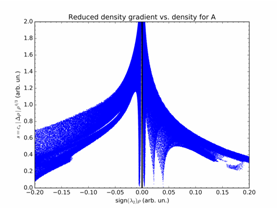
\includegraphics{image/P1-F811} & 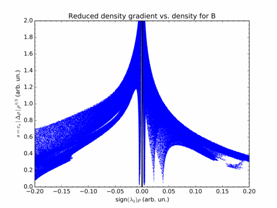
\includegraphics{image/P1-F812} & 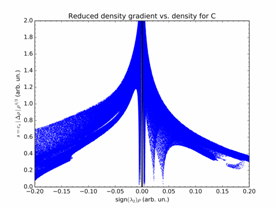
\includegraphics{image/P1-F813}\\
					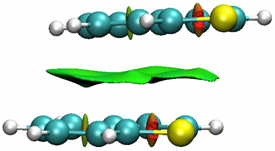
\includegraphics{image/P1-F821} & 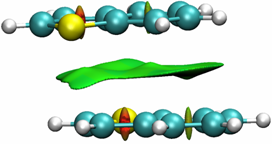
\includegraphics{image/P1-F822} & 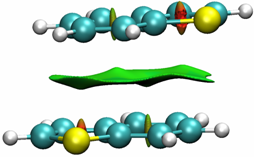
\includegraphics{image/P1-F823}\\
					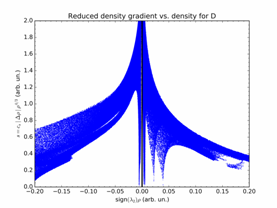
\includegraphics{image/P1-F831} & 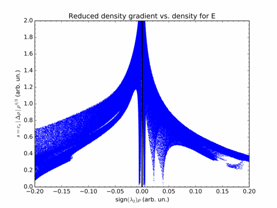
\includegraphics{image/P1-F832} & 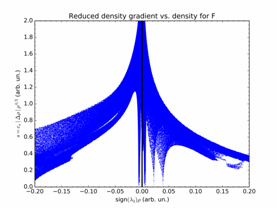
\includegraphics{image/P1-F833}\\
					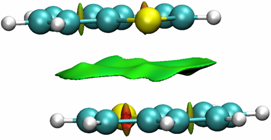
\includegraphics{image/P1-F841} & 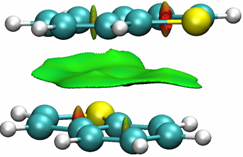
\includegraphics{image/P1-F842} & 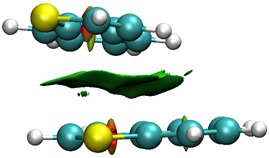
\includegraphics{image/P1-F843}\\
					\includegraphics{image/P1-F851} & \includegraphics{image/P1-F852} & \\
					\includegraphics{image/P1-F861} & \includegraphics{image/P1-F862} & \\
				\end{tabular}
			\end{center}
			\caption{Plots of the electronic reduced gradient density's against against the density $\rho$ times the sign of $\lambda_{2}$}
		\end{figure}
		
		In this Figure, the low density, high gradient regions correspond to the exponential decay of the electronic density away from the nuclei of the molecules. The regions of gradient values around 0.5 arbitrary units and density values around $\pm$ 0.2 au correspond to the covalent interactions: in the positive region this is related to the repulsive character of the covalent intramolecular bonds and the negative region is correlated with attractive character.\\
		
		Moreover, the plots of these surfaces allow one to visualize the regions of space where the interactions are stronger. The color mapping indicates their repulsive character (towards red) or attractive (toward green). The intra-ring nuclear repulsion can be clearly distinguished from the interaction surfaces between the molecules of the dimer system in this way.\\
		
		From these plots, one can deduce that the conformations of the dimers have, to a limited extent, some influence on the non-covalent interactions. Although very little can be said from the reduced density gradient versus the density plots, the non-covalent surfaces show singular features for the studied conformers: conformer \textbf{F} has attractive interactions between the hydrogen atoms of one molecule and the carbon atoms of the other while conformer H has regions where no interaction takes place or where they mutually cancel (indicated by the holes on the surface). Moreover, analysis of the positioning of the intra-ring nuclear repulsion interactions shows that systems \textbf{C}, \textbf{D} and \textbf{E} have the surfaces of each benzyl or thiophene ring in opposition to each other. This increased interaction between the planes might indicate that the translational (sliding) vibration modes of one plane over the other should be slighty shifted to higher wavenumbers.\\
		
		\textit{Very Low wavenumber region (~30–100 cm$^{-1}$):}
		
		The first conclusion to be drawn from our calculations for all conformations for all species is that the very low wavenumber features in the spectra for all of the dimers are very similar to each other.\\
		
		
		This observation is also consistent with our spectra recorded between 5 and 26 cm$^{-1}$ for the dibenzothiophene \textbf{1\textit{b}},  4,6-dimethyldibenzothiophene \textbf{1\textit{c}} and 4-methyldibenzothiophene \textbf{1\textit{d}} systems (see Figure \ref{mole-verylow}). The assignation of the six libration modes of the most stable conformers for the four species (\textbf{2\textit{a}}-\textbf{2\textit{d}}) is reported in Table 5. The parameters of the variation-perturbation calculations used for each species are also reported in this table. These results show that the modes with the lowest wavenumbers, \textit{i.e.}, the sliding mode along the $xy$ plane (Figure 7) and the rotation around the main axis perpendicular to the plane of the isolated molecules (y direction) are mainly coupled; these modes are also coupled with several CH stretching modes. On the other hand, the other libration modes and, particularly, the sixth corresponding to the $\alpha$-type rocking mode are coupled, at the same time, to the stretching and wagging $\omega_{CH}$ modes. This justifies why these modes must imperatively be present in basis $\textbf{B’}$ (or $\textbf{B’’}$) in which the variation-perturbation work is performed so that convergence can be achieved. The calculated frequencies for each one of the dimers are reported in Table 6. Moreover, the results concerning the dibenzothiophene molecule are reported in Table 7 and compared to the only experimental data available in the literature and also to our PA measurements. All the results that were gathered from the literature do not lead to the same frequency due to the different methodologies in use but rather to a dispersion (around the frequency found by us). This is unsurprising since the measurement conditions differ among these experiments. The calculations performed for the dibenzothiophene dimer are in good agreement with the ensemble of experimental observations. They confirm that the very low-intensity bands observed experimentally are indeed the signatures of the intermolecular modes. The results in Table 6 also show that the rocking modes, found between 60 and 100 cm$^{-1}$, are not strongly dependent on the specie under study, and have more intense signatures than the libration modes. The rotation and sliding modes are much less intense and their locations are more dependent on the type of molecule. They are also more difficult to characterize in all types of spectroscopy: however, we have recently identified weak infrared absorption bands that may correspond to the sliding mode in spectra acquired using coherent synchrotron radiation (Figure \ref{mole-verylow}). Finally, the presence of one or several substituents at different positions on the molecule can also change the intensity of the signatures of the libration modes significantly, particularly for those implying, through vibration, the movement of the substituents towards each other, which gives rise to new intermolecular interactions.\\
		
		Previously, our group showed the extent to which these interactions play a significant role in the aggregation of molecules constituting the asphaltenes and the importance of characterizing them.\cite{silva2016molecular} Among these interactions, a non-negligible part consists in intermolecular interactions. Characterizing them through spectroscopy is then crucial for understanding the aggregation phenomena of asphaltene mixtures and, thus, estimating the energies required to separate them during the refining process and avoid the asphaltene sedimentation phenomenon widely observed in the pipelines. Our work using molecular dynamics sheds some light on the nature of the intermolecular interactions that can take place in the mixture for different heteroatoms, different lateral chains, etc. Among our future aims is the identification of characteristic features in vibrational spectra which permit identification of each interacting species for different heteroatoms and lateral chains that may be present in these aggregated systems.\\
		
		In summary, the present work shows that: 1) solving the vibrational Schr\"{o}dinger equation for isolated molecules allows one to identify, for molecules containing the sulfur heteroatom, the vibration modes for different molecular moieties as well as their singular spectroscopic properties; 2) utilizing both IR and Raman spectroscopy is very useful towards the full identification of these modes; 3) variation-pertubation calculations in the 100-700 cm$^{-1}$ region make it possible to complete the assignment of the modes of each monomer (which was previously initiated in the literature); 4) in the same region, vibrational modes of the dimers correspond to those of the isolated molecules making it possible to determine based solely on these modes, whether the molecules are interacting or not; 5) these intermolecular interaction modes are expected only at very low wavenumbers, and 6) in the region below 100 cm$^{-1}$, each molecule containing different configurations has characteristic signatures in the vibrational spectrum: these signatures arise from the sliding or rotation modes of one molecular plane with respect to another and can be in- or out-of-phase. Even though no general rule could be established concerning the behavior of these modes for different species or configurations, it is clear that their possible existence can serve as a marker for the presence or absence of intermolecular aggregation.\\ 
		
		Additionally use of the NCI formalism on a wide range of molecules cointaining different substituents and different heteroatoms should enable us to characterize the nature of these interactions in the future, and to quantify the energies involved in these interactions. This will make it possible to predict the behaviors for different molecular architectures and heteroatom arrangements.\\
		
		
		Finally, the description of the intermolecular modes chosen in this work is a first step of a project aimed at fully characterizing the aggregation interactions. In future work, we plan to a) perform solid state calculations, which are closer to actual experimental conditions since these interaction modes are linked to the deformations of the crystalline network of the solid (related results were already published by our group concerning the vibrational modes near 100 cm$^{-1}$ for a family of acenes); and b) study families of molecules with different chemical substituents and different heteroatoms (N, O and S).
		
		\begin{table}[H]
			\caption{Parameters used in the variation-perturbation process (values of X’ and Y as defined in Figure \ref{P1-fig2} parameters and dimension of of the variational  problem $\textbf{B’’}$) for each intermolecular mode of the four most stable dimers \textbf{2a-2d}}
			\begin{center}
				\resizebox{17.2cm}{!}{
					\begin{tabular}{c c c c c c c c c}
						\toprule
						& \multicolumn{2}{p{4cm}}{\centering \textbf{Benzothiophene}} & \multicolumn{2}{p{4cm}}{\centering \textbf{Dibenzothiophene}} & \multicolumn{2}{p{4cm}}{\centering \textbf{4-methyl} \\ \textbf{dibenzothiophene}} & \multicolumn{2}{p{4cm}}{\centering \textbf{4,6-dimethyl} \\ \textbf{dibenzothiophene}}\\
						Mode & type & X’’ ; Y’’ ; $\textbf{B’’}$ & type & X’’ ; Y’’ ; $\textbf{B’’}$ & type & X’’ ; Y’’ ; $\textbf{B’’}$ &type & X’’ ; Y’’ ; $\textbf{B’’}$\\ 
						\\
						1 & $x$,$y$  & 1 ; 7  ; 2500 & $\gamma$            &  1 ; 10 ;  3200 & $\gamma$            &  1 ; 14 ;  8100 & $\gamma$            &  1 ; 17 ; 10300 \\
						2 & $\gamma$ & 3 ; 7  ; 2500 & $x$,$y$             &  3 ; 10 ;  4100 & $x$,$y$             &  3 ; 14 ;  9000 & $x$,$y$             &  3 ; 17 ; 15100 \\
						3 & $x$,$y$  & 5 ; 7  ; 3000 & $x$,$y$             &  5 ; 10 ;  4500 & $x$,$y$             &  5 ; 14 ; 10500 & $x$,$y$             &  5 ; 17 ; 16600 \\
						4 & $\alpha$ & 7 ; 12 ; 3600 & $\alpha$            &  7 ; 15 ;  8800 & $\alpha$            &  7 ; 20 ; 12700 & $\alpha$            &  7 ; 23 ; 20500 \\
						5 & $\beta$  & 3 ; 12 ; 3500 & $\beta$             &  3 ; 15 ;  6300 & $\beta$             &  3 ; 20 ;  9900 & $\beta$             &  3 ; 23 ; 17400 \\
						6 & $\alpha$ & 9 ; 12 ; 4200 & $\alpha$ + $\omega$ & 11 ; 15 ; 15000 & $\alpha$ + $\omega$ & 11 ; 20 ; 17200 & $\alpha$ + $\omega$ & 11 ; 23 ; 24900 \\
						\bottomrule
					\end{tabular}}
				\end{center}
			\end{table}
			
			
			\begin{table}[H]
				\caption{calculated intermolecular vibrations modes of the four most stable dimers \textbf{2a-2d}}
				\begin{center}
					\resizebox{17.2cm}{!}{
						\begin{tabular}{c c c c c c c c c}
							\toprule
							& \multicolumn{2}{p{4cm}}{\centering \textbf{Benzothiophene}} & \multicolumn{2}{p{4cm}}{\centering \textbf{Dibenzothiophene}} & \multicolumn{2}{p{4cm}}{\centering \textbf{4-methyl} \\ \textbf{dibenzothiophene}} & \multicolumn{2}{p{4cm}}{\centering \textbf{4,6-dimethyl} \\ \textbf{dibenzothiophene}}\\
							Mode &  $\omega^{a}$ (I)$^{b}$ & $\nu^{a}$ & $\omega^{a}$ (I)$^{b}$ & $\nu^{a}$ & $\omega^{a}$ (I)$^{b}$ & $\nu^{a}$ & $\omega^{a}$ (I)$^{b}$ & $\nu^{a}$\\
							\\
							1 & 17 (0.02) &   &  18 (0.05) &  &  22 (0.01) &  &  17 (0.00)  &  \\
							2 & 18 (0.08) &  & 28 (0.01) & 24 & 36 (0.17) & 32 & 22 (0.01) & \\
							3 & 45 (0.06) & 39 & 36 (0.09) & 35 & 37 (0.01) & 31 & 41 (0.01) & 38\\
							4 & 67 (0.32) & 58 & 70 (0.32) & 66 & 65 (0.07) & 55 & 74 (0.52) & 66\\
							5 & 74 (0.02) & 67 & 89 (0.01) & 82 & 81 (0.03) & 67 & 83 (0.07) & 69\\
							6 & 91 (0.06) & 88 & 93 (0.56) & 92 & 96 (0.06) & 85 & 84 (0.01) & 78\\
							\bottomrule
						\end{tabular}}
						
						\begin{tablenotes}
							\item[a] : cm$^{-1}$
							\item[b] : km/mol
						\end{tablenotes}
					\end{center}
				\end{table}
				
				
				
				
				\begin{table}[H]
					\caption{Experimental and calculated intermolecular vibration modes (cm$^{-1}$) of dibenzothiophene dimer (\textbf{B}) }
					\begin{center}
						\begin{threeparttable}[b]
							\begin{tabular}{c c c c c c c c}
								\toprule
								& \multicolumn{2}{p{5cm}}{\centering \textbf{$\omega$B97x-D/6-311++G**}} & & & \textbf{IR$^{a}$} & \textbf{Raman$^{a}$} & \multicolumn{1}{p{2.5cm}}{\centering \textbf{IR$^{b}$} \\ \textbf{}}\\
								Mode & $\omega$ (I)$^{c}$ [I$^{Raman}$]$^{d}$ & $\nu$ & & & \multicolumn{3}{p{6cm}}{\centering $\nu$}\\
								\cline {1-3} \cline{6-8}
								\\
								1 & 18 (0.05) [0.62] &    & & &            &           &       \\
								2 & 28 (0.01) [7.96] & 24 & & &            &           &       \\
								3 & 36 (0.09) [9.15] & 35 & &  &53 w        & 48 - 49   & 56 w  \\
								4 & 70 (0.32) [0.51] & 66 & & &72 w        & 63        & 69 vw \\
								5 & 89 (0.01) [0.51] & 82 & & &89 vw       & 79 - 82   & 78 vw \\
								6 & 93 (0.56) [3.33] & 92 & & &104 - 101 w & 103 - 106 & 88 vw \\
								&                  &    & & &109 w       & 126       &       \\
								\bottomrule
							\end{tabular}
							
							\begin{tablenotes}
								\item[a] : liquid/crystal ref\cite{bree1971vibrations}.
								\item[b] : this work (crystal) 
								\item[c] : km/mol
								\item[d] : A$^{4}$/AMU
							\end{tablenotes}
						\end{threeparttable}
					\end{center}
				\end{table}
				
				\begin{figure}[H]
					\centering
					\subfigure[dibenzothiophene]{\includegraphics[scale=0.45]{image/dibenzo-verylow}}
					\subfigure[4,6-dimethyldibenzothiophene]{\includegraphics[scale=0.45]{image/4m-verylow}}
					\subfigure[4-methyldibenzothiophene]{\includegraphics[scale=0.45]{image/46m-verylow}}
					\caption{Far-infrared spectra of dibenzothiophene \textbf{1\textit{b}}, 4,6-dimethyldibenzothiophene \textbf{1\textit{c}} and 4-methyldibenzothiophene \textbf{1\textit{d}}. Data were acquired using coherent synchrotron radiation and a Bruker IFS 125HR FT-IR spectrometer.}  \label{mole-verylow}
				\end{figure}
	
	
\newgeometry{textwidth=16cm}
\chapter[Vibrational spectra calculations]{Heteroatoms}
\minitoc
\restoregeometry

\newpage
	
	
	\section*{Introduction}


The chemical complexity of asphaltenes, which represent the heaviest fraction of oil, make their analysis and modelling very challenging, since the detailed molecular composition remains up to now unknown. However, some studies have reported that they consist of a heterogeneous mixture of polycondensed molecules, containing heteroatoms $X$ such as sulfur, oxygen, and nitrogen. On the other hand, vibrational spectroscopy has shown to be a tool for the identification and characterization of molecules in ill-defined mixtures, in combination with predictive modelling.\\

Considering this, in this chapter, the far- and mid-infrared spectra of a series of heteroaromatic (N, O and S) hydrocarbons and their dimers have been calculated using Density Functional Theory (DFT) within the $\omega$B97X-D/6-311++G** level of theory. The perturbational-variational method presented in the previous chapter coupled with potential truncation was incorporated in order to provide anharmonic corrections of monomers. Identification and quantification of peaks from \textit{inter} and \textit{intra}-molecular vibrations in experimental spectra have been performed. Also, experimental IR bands in the far-IR region were identified, allowing the differentiation of the \textit{inter}-molecular and \textit{intra}-molecular vibrations. In addition, the interaction energies were studied using DFT-SAPT\footnote{The symmetry-adapted perturbation theory based on density functional theory) at the PBE0/aug-cc-pVTZ level of theory.} \\
	
	These methods reproduce energies in the same order of magnitude and identify $\pi-\pi$ stacking as the dominant electronic interaction. Understanding the interaction between these primary units helped us to enrich the knowledge of the \textit{inter} and \textit{intra}molecular interactions in asphaltenes and why they tend to aggregate and then flocculate from the oil condensed phase. This outcome illustrates that the spectral signatures of heteroaromatic compounds can be used to probe the molecular and sub-molecular composition, and the \textit{inter}-molecular interactions present in asphaltenes by spectral decomposition.\\
	
	
	\section{Structural details}
	
	The molecular structures of thiophene, benzofuran, carbazole and fluorene-like molecules and their respective dimers were calculated using Density Functional Theory (DFT) with the $\omega$B97X-D exchange-correlation functional and the   6-311++G** basis set, implemented in the Gaussian 09 suite of programs. The $\omega$B97X-D functional developed by Chai \textit{et al}\cite{chai2008systematic} is based on optimized long-range corrected hybrid density functionals, which employ 100\% Hartree-Fock (HF) exchange for long-range electron-electron interaction correction. This method, tested by Salzner \textit{et al}\cite{salzner2011improved} for $\pi$-conjugated oligomers, was also benchmarked successfully for interacting polycondensed aromatic molecules,\cite{spillebout2014discerning} thus proving it overcomes the failure of standard DFT calculation approaches to describe long-distance interactions. The 6-311++G** basis set is of triple-zeta quality for the valence electrons. Among the basis sets tested by Wiberg,\cite{wiberg2004basis} including the Dunning correlation basis sets such as aug-cc-pVTZ and aug-cc-pVQZ, the 6-311++G** basis set gave accurate geometries and frequencies at a relatively small computational cost. The geometrical parameters of the molecules are benchmarked with experimental data when available.\\
	
	
	For dimers, as an alternative to the supermolecular treatment, an approach based on symmetry-adapted perturbation theory (SAPT)\cite{jeziorski1994perturbation} which utilizes the description of the interacting monomers in terms of Kohn-Sham (KS) orbitals was used in this work. The DFT-based SAPT approach,\cite{hesselmann2005density} denoted herein as SAPT-DFT, is exact for all major components of the interaction energy (asymptotically for exchange interactions) in the sense that these energies would be exact if the DFT description of the monomers were exact. The SAPT-DFT calculations were performed using the MOLPRO2012 package.\cite{MOLPRO_brief} The PBE0 functional\cite{adamo1999toward} was used as a monomer DFT functional in SAPT, using the aug-cc-pVTZ basis set. 
	
\section{Results and Discussion}


\subsection{Global analysis}

The methodology behind this part of the work is close to that of the ‘design of experiments’ \cite{goupy2013introduction}. Indeed, studying all the moieties, all the heteroatoms, all the substituents as well as all the allowed \textit{inter}-molecular associations of the hypothetical constituents of the asphaltenes (for which, \textit{cf.} chapter 1, both the composition and formulation are unknown) is utopic and unrealistic. The general principles behind the approaches of the type “design of experiments” rely on the organisation and limitation of the experiments/calculations when a link between a response function $y$ and variables $x_i$ (designated a ‘factor’) is sought after. Within the context of this work, the searched response function is knowing whether or not, for any given compound constituted of a given moiety, presenting or not an heteroatom, interacting or not among them, owns an active vibrational signature. These three criteria represent the three principle factors taken into account in our calculations. Unluckily, our problem is more complex since, besides being active, this vibrational mode should also be identifiable within a spectral zone where the density of modes is weak enough to avoid hiding the signature that is looked for. The notion of spectral zone is the last factor that has been considered in this study.\\

Actually, we also could have multiplied the chemical moieties \textit{ad infinitum} and accumulate more and more vibrational information for these systems, but it would be very complicated and hard to manage and explore all these data. We have chosen to concentrate on a strict domain of definition for which the main pieces of information are controlled so that useful information can be provided to spectroscopists:  “is it possible for a given asphaltene to use IR and Raman to characterise the presence of associated systems?” and, “is it possible to assign these signatures to the presence of the three main heteroatoms (oxygen, sulphur and nitrogen)?”\\


Infrared and Raman spectra of  indene \textbf{1\textit{a}}, fluorene \textbf{1\textit{b}}, benzofluorene \textbf{1\textit{c}}, cyclopentaphenanthrene \textbf{1\textit{d}}, 1-methyl-fluorene \textbf{1\textit{e}}, 1,8-di methyl-fluorene \textbf{1\textit{f}},
indole \textbf{2\textit{a}}, carbazole \textbf{2\textit{b}}, benzocarbazole \textbf{2\textit{c}}, 4,5 iminophenanthrene \textbf{2\textit{d}}, 1-methyl-carbazole\textbf{1\textit{e}}, 1,8-di methyl-carbazole \textbf{1\textit{f}},
benzofuran \textbf{3\textit{a}}, dibenzofuran \textbf{3\textit{b}}, benzonaphtofuran \textbf{3\textit{c}}, tribenzofuran \textbf{3\textit{d}}, 4-methyl-dibenzofuran\textbf{3\textit{e}}, 1,8-di methyl-dibenzofuran \textbf{3\textit{f}},
benzothiophene \textbf{4\textit{a}}, dibenzothiophene \textbf{4\textit{b}}, benzonaphtothiophene \textbf{4\textit{c}}, tribenzothiophene \textbf{4\textit{d}}, 4-methyl dibenzothiophene \textbf{4\textit{e}} and 4.6-dimethyl dibenzothiophene \textbf{4\textit{f}} were studied in this work. In complement, the observed bands of the monomers are assigned using high level calculations based on anharmonic electrical and mechanical approximations. All computational outcomes are reported in the annexe xx.
	
	\begin{figure}[H]
		\begin{center}
			\begin{tabular}{c c c}
				\includegraphics[scale=0.15]{image/benzo} & \includegraphics[scale=0.13]{image/dibenzo} & \includegraphics[scale=0.12]{image/benzonaphto}\\
				\textbf{1} & \textbf{2}& \textbf{3}\\
				\includegraphics[scale=0.12]{image/tribenzo-lajolie} & 
				\includegraphics[scale=0.13]{image/methyl-benzo} & \includegraphics[scale=0.13]{image/dimethyl-benzo} \\
				\textbf{4} & \textbf{5} & \textbf{6}\\
			\end{tabular}
		\end{center}
		\caption{Molecular structures studied: \textbf{a} Benzo, \textbf{b} Dibenzo, \textbf{c} Benzonaphtho, \textbf{d} Tribenzo, \textbf{e} methyldibenzo, \textbf{f} dimethyldibenzo. X= \textbf{1} C, \textbf{2} N, \textbf{3} O and \textbf{4} S.}
	\end{figure}
	
	The two first factors we studied were: 1- the nature of the heteroatom (factor $x_1$), for which the bounds were arbitrarly set to $x_{1(min)}=C$ and $x_{1(max)}=S$; 2- the nature of the chemical moeity, which is discrete and not easily quantifiable ($x_{2(min)}=benzo$ and $x_{2(max)}=tribenzo$.). The spectral zone is then a third factor to be considered and which definition is also discrete. 
	Four spectral zones were defined: the very low wavenumbers one ($x_{3(min)}=1$), which displays the signatures of the \textit{inter}-molecular modes (represented on the figures by the “$ + $” symbol), butterfly-like (“$\ocircle$”) and torsion (“$\triangle$ and $\lozenge$”) modes, which are particularly active in this region; another one ($x_3=2$), covering the signatures of the cycle breathing and scissoring (“$\lhd$”), twist (“$\triangledown$”) and wagging modes that are impacted by the presence of the hetero atom (pure: $\pentagon$, X-H: $\octagon$, wagging/carbon backbone wagging: $\square$); $x_3=3$ covering the C-X ($\varhexagon$) streching, the CCC and CXC angular deformations ($\bigstar$) modes of the aromatic cycles and the C-H wagging modes ones; and, finally, the $x_3=4$ zone covering carbon-carbon and C-H streching modes found beyond 1300 cm$^{-1}$.  A table summarizing the modes that are followed in this study as well as their respective symbols is presented in Figure XX. The modes of interest and which are represented in our Figures by the use of pictograms are the ones for which the hetero atom contribution is strong for the ensemble of the 24 studied molecules, in average. The last factor considered in this work concerns the presence ($x_{4(min)}=yes$) or not ($x_{4(max)}=no$) of \textit{inter}-molecular interactions by analysing the dimers and monomers, respectively. However, one should note that this chapter only reports the results of the work done in the molecular state for which the only aim is defining if it is relevant to consider one or several spectra signatures (\textit{intra}- and \textit{inter}-molecular) that could allow one to characterise the heteroatoms present in the asphaltene mixtures and their associated vibrational modes. In chapter XXX, the description of the \textit{inter}-molecular modes will be discussed in more details by the development of solid state calculations taking into account this time of the global environment of the studied systems.\\
	
	The implementation of an “ordered” strategy able to take into account the characteristics discriminating spectroscopically all the systems is justified when one take a look at Figure \ref{figP2-2}. In this figure, the ensemble of the calculated modes of the 24-monomer systems is reported without distinction neither of the spectral zone nor the intensity. We can easily realise the extent of the data available to treat this problem. Only the modes for which the heteroatom is directly implied  in the development of a given vibration are reported in Figure \ref{figP2-2} as colored points.
	
	
	\begin{figure}[H]
		\begin{center}
			\includegraphics[scale=0.7]{image/P22}
		\end{center}
		\caption{Vibration modes heteroatoms contributions > 5\% for studied molecules.} \label{figP2-2}
	\end{figure}
	
Several pieces of informations can be extracted from this figure. First of all, the number of modes having an influence of the heteroatom X = C, N and O is of the order of 50\% of all the modes, regardless of the molecule. This percentage is reduced by half for the molecules of the thiophene family.The contributing modes are, in this case, concentrated in the low wavenumber spectral zones ($x_3=1$ and 2 – what is due to a simple mass effect). This first analysis also shows that within the three first spectral zones localised below 1300 cm$^{-1}$ there are much more similarities between the signatures of $x_1=N$ and $O$ heteroatoms than there are between $S$ and $C$. Lastly, and except for sulfur, it is clear that below 1000 cm$^{-1}$ the signature of each moiety is singular. This observation is particularly pronounced in the lowest spectral zone $x_3=1$, where the torsion and deformation modes of the backbone can be found (including, this time, the thiophenic molecules). The moiety seems to be, at this stage, a major discriminatory criterion of the spectral signature of these molecules. 
	
	
	
	
		\begin{figure}[H]
			\begin{center}
				\includegraphics[scale=0.7]{image/P2-3}
			\end{center}
			\caption{Vibration modes heteroatoms contributions > 5\% for dimers configurations}  \label{figP2-3}
		\end{figure}
	
	
In figure \ref{figP2-3}, the same information reported in figure 2 is presented for the ensemble of the most stable dimer of each specie. Figure \ref{figP2-2} and \ref{figP2-3} look alike apart from the emergence of \textit{inter}-molecular modes at very low wavenumbers for which the contribution of the hetero atoms are strong. Another remarkable difference concerns the nitrogen heteroatom since it seems that it is the only one with a density and rate of contributing modes evolving. This is particularly true for the zones $x_3=1$ around 150 cm$^{-1}$ and $x_3=2$ around 400-500 cm$^{-1}$. No other significant difference can be highlighted from figure \ref{figP2-3}. This corroborates the idea stating that the signatures of the \textit{intra}-molecular modes specific to each molecule constituting the dimers are, except these two precedent observations, the very same reported for the monomers. 
Another difference that can be noted is the spectral behaviour of the 24 molecules within the study domain depiced in Figure \ref{figP2-4}. In this figure the spectral signatures taking into account the intensities and filtrated by each moiety are reported. For each one of them, one can observe again at the lowest frequencies a singular behaviour of the signatures associated to the molecules of the carbazol family. The modes associated seem to own more intense signature for which the position seems to depend on the moiety more than for any other heteroatom.	
	
	
	\begin{figure}[H]
		\begin{center}
			\includegraphics[scale=0.5]{image/P2-4}
		\end{center}
		\caption{Calculated vibrational spectra for all molecules, motifs and heteroatoms comparisons. }  \label{figP2-4}
	\end{figure}
	
Another information concerns now the thiophene family of molecule. If in figure \ref{figP2-2} and \ref{figP2-3} one could verify a non-negligible translation of contributing modes towards the low-wavenumber zone, figure \ref{figP2-4} shows that, in the 700-1600 cm$^{-1}$ (sparsely populated, though) the activity of the remaining modes have not (or very little) lowered in comparison to the equivalent signatures observed for the other hetero atoms (for those, there are no sparsely populated region). The reason behind it is very simple: the majority of the remaining modes imply vibrations of the carbonic backbone that are not very dependant on the hetero atom and are common to all moieties. In this way, it is clear that this spectral zone is of no (or a little) interest to discriminate the spectral behaviours of the different systems. The $x_3=3$ zone is also not very well suited to the discrimination of the vibrators, since it concentrates the most active modes (common to all systems) which the amplitude of the signals can hide all the other signatures. Finally, zones $x_3=1$ and $2$ seem to be more adapted to this discrimination. A finer analysis, mode per mode of these two spectral zones is still necessary in order to identify the singularities of each moiety and each hetero atom, what is reported hereafter.

\subsection{Analyse}

At this point, we should remember that such analysis has a sense only if one tries to product a global information of the spectral behaviour of the molecules (or moieties) potentially present in asphaltenes and, particularly, the signatures of \textit{inter}-molecular signatures on the basis of the samples of chosen model molecules. Of course, if we had the exact formulation of the molecules present in the asphaltenic medium available, it would suffice to model the spectrum of each molecule, for every single moiety and every single heteroatom in order to find, for each molecule, one or several singular characteristics able to discriminate it among the others. Employing mathematical methods dedicated to the resolution of the vibrational Schr\"{o}dinger equation such the ones already presented in chapter XX (developed within the anharmonic hypothesis) would be enough to provide to spectroscopists useful information (fundamental bands, combination bands, overtones, medium and near IR, Raman, …) The full description of the 24 molecules studied in this work can be found in the Appendix of the manuscript.\\  

The afore reported analysis allows one to bring to light the singular behaviours linked to the presence of heteroatoms and the associated molecules. Despite the fact that this analysis is qualitative and does not allow to conclude concerning the role of each factor. A more detailed analysis of the different modes implicated in each molecule was then necessary to address this problem. In view of the very specific role that the nitrogen hetero atom seem to play, a first detailed study of the carbazole molecule is presented, for which experimental data is available. This will be followed by a second one performed on the dibenzothiophene molecule for which exhaustive experimental data is also available. We should finish by resuming the ensemble of data for each one of the 24 molecules studied in this work, focusing on the differences observed in the $x_3=1$ and $2$ spectral zones (which were previously identified as the one allowing one to discriminate plus efficiently the role of each moiety and heteroatom on the association process).	

\section{Carbazole}

The molecules of the carbazole family are the ones for which the heteroatom contribution to the vibrational modes are the strongest. Another particularity of this family is that the most intense contributions can be found in the lower zones of the spectra. The carbazole monomer presented in figure \ref{figP2-5} depicts these observations. 

 \begin{figure}[H]
 	\begin{center}
 		\includegraphics[scale=0.8]{image/P2-5}
 	\end{center}
 	\caption{Atomic percentage contributions to vibrational modes in Carbazole molecule.} \label{figP2-5}
 \end{figure}
	
	
	

	
	Similarly, it becomes clear from this picture that the variations of heteroatom contributions spread over the three spectral zones $x_3=1-3$ and are, exception made to mode 4 ($\omega_{N-H}$), perfectly correlated to the contributions linked to the case where carbon is the heteroatom. These three spectral zones, distributed over around 900 cm$^{-1}$, characterise the ensemble of the signatures of the 25 first modes of carbazole. Among these 25 modes, those for which the contribution of the heteroatom is the most important are repported in figure \ref{figP2-6} by the aforementioned pyctograms. One can note that, except the C-X stretching mode ($\varhexagon$), all the modes depicted by pictograms can be found for carbazole. This information is not enough to allow a rigorous analysis of carbazole’s spectrum. To do so, it is also necessary to take into account at the same time the intensity of each mode and having in hand simultaneously the equivalent information for the dimer molecules if one wishes to characterise the signatures of the \textit{inter}-molecular modes. The ensemble of these pieces of information is reported in Figure \ref{figP2-7}.
	 
	 
	\begin{figure}[H]
		\begin{center}
			\includegraphics[scale=0.6]{image/P2-6}
		\end{center}
		\caption{Calculated vibrational spectra of Carbazole molecule, showing heteroatom contribution and important modes.}  \label{figP2-6}
	\end{figure}
	

	
	
	The information present in this picture reveals several distinct signs of monomeric and associated carbazole. 1 – a first category of modes seems to distinguish themselves from the others, i.e., those which have a strong contribution of the hetero atom and a strong intensity at the same time. For instance, carbazole’s first modes to own the two characteristics are the twist ($\triangledown$) and wagging ($\square$) ones, found between 550 and 600 cm$^{-1}$. Even if the response of these modes seems to be the most accessible of a spectroscopic point of view, we also could realise that these characteristics are also identically present for the simulations of carbazole dimers. Because of these strong similarities, these modes are thus not useful to our analysis. 2- the presence of \textit{inter}-molecular modes is, on the other hand, more useful. This has been brought to light by our calculations based on the appearing of low intensity signatures at very low wavenumbers which positioning, at least apparently, agrees well with the experimental data reported by K. Michaelin and J. Shaw (figure \ref{figP2-8}). We shall present in this chapter only the results of these specific modes. The quantical treatment of these \textit{inter}-molecular modes will be the subject of development in chapter XX of this work. However, we should note that these modes are particularly coupled with the others of the deformation type, such as the “butterfly” mode ($\ocircle$). 
	 Consequently, these couplings induce the presence of distinctive differences between the signatures of the monomers and of the dimers within the region nearby the one associated to the \textit{inter}-molecular modes, as it is depicted in Figure \ref{figP2-8}. This is then a zone of interest to us that shall need a very precise description when we will model the vibrational signatures of the systems at the solid state (chapter XX).
	 
	 
	 	\begin{figure}[H]
	 		\begin{center}
	 			\includegraphics[scale=0.5]{image/P2-7}
	 		\end{center}
	 		\caption{Calculated vibrational spectra of Carbazole monomer and dimer, between 0- 800 cm$^{-1}$, showing heteroatom contribution and important modes.}  \label{figP2-7}
	 	\end{figure}
	 	
	 		\begin{figure}[H]
	 			\begin{center}
	 				\includegraphics[angle=90,scale=0.32]{image/8}
	 			\end{center}
	 			\caption{Comparison between calculated vibrational spectra of monomer and dimer with IR experimental at 0- 250 cm$^{-1}$ of Carbazole} \label{figP2-8}
	 		\end{figure}
	 		
	 		
	 \subsection{}
	
	another category of modes that are specific to the carbazole family will allow us to highlight the presence of moieties associated as shown by the experiments conducted by K. Michaelian. So that the characterisation of these specific modes can be done, we have reported in figure 9 the evolution of the density of vibrational states against the vibrational frequencies for carbazole’s monomer and dimer. It appears distinctly in figure \ref{figP2-9} two zones with strong densities within the zone $x_3=2$ (comprised between 250-500 cm$^{-1}$) that should indicate strictly the presence of two spectral zones in the experimental spectrum. Yet, one can found in this spectrum only intense zone centered at 450 cm$^{-1}$. Nevertheless, a very weak activity is noted around 300 cm$^{-1}$, precisely at the same place where there is a strong density of vibrational states. 
	
	\begin{figure}[H]
		\begin{center}
			\includegraphics[angle=90,scale=0.5]{image/9}
		\end{center}
		\caption{Comparison of density of modes at low wavenumber region of Carbazole.}  \label{figP2-9}
	\end{figure}
	
	
	Our calculations also show that all the dimer’s modes (however more numerous than those of the monomers in this zone) present around 300 cm$^{-1}$ are practically all inactive. On the other side, if the density of modes for the monomer in this region is weaker than the one of the dimer, the 280-300 cm$^{-1}$ zone remains potentially the place where detectable signatures could be found for this specie (as it is depicted in figure \ref{figP2-7}). The analysis of a second regions centred at 450 cm$^{-1}$ reveals this time that two species (monomer and dimer) have both of them a stronger density of modes, but oppositely to the dimer, no monomer’s vibration mode localised within this region have a strong signature. Another very important information concerns the N-H wagging modes ($\pentagon$ and $\octagon$)
	  at the origin of monomer’s spectral signature in the 280-350 cm$^{-1}$ zone. As a result of the presence of \textit{inter}-molecular interactions, the position of these modes is strongly displaced towards higher wavenumbers for the dimer. Surprisingly, they are displaced to around 450 cm$^{-1}$, what induces an augmentation of the dimer’s modes density in this region. Experimentally, this region is where a strong, wide spectral band having several bumps can be found and this seems to agree well with what was calculated for the associated specie (and reported in figure \ref{figP2-10}, on which the modes’ intensities are also shown alongside their densities). Moreover, the 280-350 cm$^{-1}$ zone is here the experimental spectral signatures are weak and this corroborates a little more the fact that carbazole is not present as a monomer (at least not predominantly)  when the spectrum was recorded.
	 
	 	\begin{figure}[H]
	 		\begin{center}
	 			\includegraphics[angle=90,scale=0.5]{image/10}
	 		\end{center}
	 		\caption{Comparison of calculated vibrational spectra and experimental data taking into account theoretical intensities for Carbazole.}  \label{figP2-10}
	 	\end{figure}
	 
	 Given the fact that we do not have experimental data for the other molecules of the carbazole family, we can not verify the validity of our hypothesis for all the species. But we can report the shifts of the N-H wagging modes predicted by our calculations and show that they are not specific to the carbazole system only for the family having nitrogen as the heteroatom (figures \ref{figP2-11ad}). Yet, the spectra reported in figures \ref{figP2-11ad} clearly show that the shifts of the wagging modes signatures are not all equivalent and apparently they strongly depend on the system in question. In figure 1\ref{figP2-12}, the pieces of information concerning these shifts were regrouped aiming to find an explanation concerning the influence of the substituent or the moiety. Unluckily, no direct link connecting the intensity of these shifts and any particular symmetry of these moieties, or the position of the substituent in the molecule, the number of them, etc, for instance, could be found. On the other hand, these results clearly show that these shifts concern only the species of the carbazole family. A deeper study will then be presented in the following paragraphs. 
	
	
	\begin{figure}[H]
		\begin{center}
			\resizebox{17cm}{!}{
			\begin{tabular}{c c}
				\includegraphics[scale=0.3]{image/P2-11a} & \includegraphics[scale=0.3]{image/P2-11b} \\
				\includegraphics[scale=0.3]{image/P2-11c} & \includegraphics[scale=0.3]{image/P2-11d}\\
		\end{tabular}}
	\end{center}
		\caption{Comparison between momoner and dimer calculated vibrational spectra for \textbf{a} Indole, \textbf{b} 4,5-iminophenanthrene, \textbf{c} 1-methylcarbazole and \textbf{d} 1,8-dimethylcarbazole at 0- 800 cm$^{-1}$ interval.} \label{figP2-11ad}
	\end{figure}
	
	
	\begin{figure}[H]
		\begin{center}
			\includegraphics[scale=0.33]{image/P2-12}
		\end{center}
		\caption{Variation of D and I modes between monomer- dimer of studied molecules} \label{figP2-12}
	\end{figure}
	
	
	In summary, two type of modes characteristic to the associated systems bearing nitrogen as the heteroatom were highlighted in our work: they are \textit{inter}-molecular modes localised at very low wavenumbers and N-H wagging modes for which the frequency, \textit{in fine}, strongly depends on the presence or not of \textit{inter}-molecular interactions. 
	
	
	
	\section{Dibenzothiophene}
	
	
	For dibenzothiophene monomer and dimer, their results are very similar for what concerns the frequency, intensity and sulphur contribution to all the vibrations. The only exceptions are the particularities listed for the nitrogen as heteroatom case (N-H wagging).
	
	
	\begin{figure}[H]
		\begin{center}
			\includegraphics[scale=0.4]{image/P2-13}
		\end{center}
		\caption{Monomer and dimer comparison of calculated vibrational spetra of Dibenzothiophene} \label{figP2-13}
	\end{figure}
	
		Analysing the 0-800 cm$^{-1}$ spectral zone for which we had particularly noted modifications (on frequencies and intensities) due to the wagging of nitrogen shows now no particularity when we have sulphur as hetero atom, neither for frequency’s positioning (figure \ref{figP2-14}) nor mode densities (figure \ref{figP2-15}). In any case and for all the spectral zones, there is an excellent theory-experiment agreement. The strong similarities found for dibenzothiophene’s monomer and dimer show that it is probably not possible to discriminate spectroscopically the presence of associated systems, exception made for the spectral zone $x_3=1$ relative to the \textit{inter}-molecular modes and the ones coupled to them, such as the butterfly ones).
	
	
		\begin{figure}[H]
			\begin{center}
				\includegraphics[scale=0.4]{image/P2-14}
			\end{center}
			\caption{Calculated vibrational spectra of Carbazole monomer and dimer, between 0- 800 cm$^{-1}$, showing heteroatom contribution and important modes.} \label{figP2-14}
		\end{figure}
		
		
			\begin{figure}[H]
				\begin{center}
					\includegraphics[scale=0.31]{image/P2-15}
				\end{center}
				\caption{Comparison between monomer, dimer calculated and experimental spectra, Densite of modes at the top and normal vibrational modes and IR intensities at the bottom.} \label{figP2-15}
			\end{figure}
	

	These ensembles of conclusions are also valid for all the other molecules of the thiophene family (figure \ref{figP2-16ad}). They also apply to the ensemble of molecules studied in this work having oxygen or carbon as heteroatom (figure \ref{figP2-17ae} and \ref{figP2-18ae}). Finally, apart the \textit{inter}-molecular modes and the ones that are coupled with them, only the N-H wagging mode for the molecules of the nitrogen family have enough singularities to allow the discrimination of the monomeric and associated states.
	
		
		\begin{figure}[H]
			\begin{center}
				\resizebox{17cm}{!}{
					\begin{tabular}{c c}
						\includegraphics[scale=0.3]{image/P2-16a} & \includegraphics[scale=0.3]{image/P2-16b} \\
						\includegraphics[scale=0.3]{image/P2-16c} & \includegraphics[scale=0.3]{image/P2-16d}\\
					\end{tabular}}
				\end{center}
				\caption{Comparison between momoner and dimer calculated vibrational spectra for \textbf{a} Benzothiophene, \textbf{b} Tribenzothiophene, \textbf{c} 4-methyldibenzothiophene and \textbf{d} 4,6-dimethyldibenzothiophene at 0- 800 cm$^{-1}$ interval.}  \label{figP2-16ad}
			\end{figure}
	
	
	\begin{figure}[H]
		\begin{center}
			\resizebox{17cm}{!}{
				\begin{tabular}{c c}
					\includegraphics[scale=0.3]{image/P2-17a} & \includegraphics[scale=0.3]{image/P2-17b} \\
					\includegraphics[scale=0.3]{image/P2-17c1} & \includegraphics[scale=0.3]{image/P2-17c}\\
					\includegraphics[scale=0.3]{image/P2-17d} & \includegraphics[scale=0.3]{image/P2-17e}\\
				\end{tabular}}
			\end{center}
			\caption{Comparison between momoner and dimer calculated vibrational spectra for \textbf{a} Benzofuran, \textbf{b} Dibenzofuran, \textbf{c} Benzonaphthofuran, \textbf{d} Tribenzofuran, \textbf{e} 4-methyldibenzofuran and \textbf{f} 4,6-dimethyldibenzofuran at 0- 800 cm$^{-1}$ interval.} \label{figP2-17ae}
		\end{figure}
		
		
			\begin{figure}[H]
				\begin{center}
					\resizebox{17cm}{!}{
						\begin{tabular}{c c}
							\includegraphics[scale=0.3]{image/P2-18a} & \includegraphics[scale=0.3]{image/P2-18b} \\
							\includegraphics[scale=0.3]{image/P2-18c} & \\ \includegraphics[scale=0.3]{image/P2-18d}&
							\includegraphics[scale=0.3]{image/P2-18e}  \\
					\end{tabular}}
					\end{center}
					\caption{Comparison between momoner and dimer calculated vibrational spectra for \textbf{a} Indene, \textbf{b} Fluorene, \textbf{c} Cyclopentaphenanthrene, \textbf{d} 1-methylfluorene and \textbf{e} 1,8-dimethylfluorene at 0- 800 cm$^{-1}$ interval.} \label{figP2-18ae}
				\end{figure}
		
		

	

\newgeometry{textwidth=16cm}
\chapter[Network modes identification]{Network modes identification}
\minitoc
\restoregeometry

\newpage


%-------------------------------------------------------------------------------------------------------------------------
%-------------------------------------------------------------------------------------------------------------------------
%-------------------------------------------------------------------------------------------------------------------------
\section*{Introduction}
\markright{INTRODUCTION}{}
%-------------------------------------------------------------------------------------------------------------------------
%-------------------------------------------------------------------------------------------------------------------------
%-------------------------------------------------------------------------------------------------------------------------

The aim of the present chapter is to perform high-precision quantum mechanical calculations to compute spectra for systems in solid state in order to characterize the signature of the inter molecular vibration for a large variety of aromatic compounds.\\

First, acenes, a family of linear polynuclear aromatic compounds possessing only $\pi-\pi$ interactions \cite{campbell1962crystal,mattheus2001polymorphism,brock1982temperature,facelli1993determination,brock1990temperature}, for which high precision experimental data are available up to pentacene \cite{michaelian2012far}, comprise a first benchmark example of this chapter that illustrates both the potential and the computational challenges found in this line of inquiry.\\

Second, additional calculations were performed for other compounds of the acene family, as well as other systems of the aromatic polycycle molecules family. The aim of these additional calculations is verifying if the position and activity of the network modes identified for the acene molecules in the solid state, and particularly the more active mode, depend on the size, length, the moiety or on the presence of hetero elements of the polycycle system in study.\\



%-------------------------------------------------------------------------------------------------------------------------
%-------------------------------------------------------------------------------------------------------------------------
%-------------------------------------------------------------------------------------------------------------------------
\section{Computational details}
%-------------------------------------------------------------------------------------------------------------------------
%-------------------------------------------------------------------------------------------------------------------------
%-------------------------------------------------------------------------------------------------------------------------


Spectral assignments, determined on the basis of both wavenumber and relative intensity values, has already been made primarily using computed spectra for individual molecules, and dimers \cite{spillebout2014discerning}.
Figure \ref{figure9}, derived from this work, gives a direct comparison of experimental and calculated spectra. Unfortunately,in this study both calculations and experiments do not give information about very low-wavenumbers and no real assignment of the inter molecular modes has been achieved. However, this experimental information exist. Far-infrared spectra provide information about intermolecular and inter-ring interactions and about $\pi$-stacking in particular. For example, by using coherent synchrotron radiation it is now becoming possible to make experimental photoacoustic IR measurements in the range 7 to 30 cm$^{-1}$ as demonstrated recently by Billinghurst and Michaelian\cite{billinghurst2010photoacoustic}. Concerning acene, Hineno \textit{et al} \cite{hineno1975far}  measured spectra of naphthalene and anthracene in the region 190-50 cm$^{-1}$ at liquid helium temperature. In the same way, bands in the experimental vibrational spectra of tetracene and pentacene that cannot be interpreted by Hineno \textit{et al} \cite{hineno1975far} based on computed wavenumbers for a single molecule are expected to arise from lattice modes. the failure of these calculations is normal. The accurate description of these network modes requires solid state calculations. In this chapter we propose to use this approach in order to describe these network modes. These calculations were finally carried out with the use of two approaches:\\



First, the calculations were carried out with the projector augmented wave (PAW) implementation of Vienna Ab initio Simulation Package (VASP) \cite{kresse1996efficient}. The generalized gradient approximation (GGA) in the PBE parameterization was considered as the exchange correlational functional \cite{perdew1996generalized}. Structural optimizations (triclinic tetracene crystal) were achieved by setting the convergence criteria for total energies below $5*10^{-6}$ eV, residual forces to be less than $1*10^{-3}$ eV/Å, and stresses limited to 0.02 GPa. To correct the missing dispersion interactions, we have used several recently proposed methods such as PBE functional with pair potential methods D2, D3 (BJ), TS, and TS+SCS. The details of the implementations and usage of these methods can be found elsewhere \cite{grimme2006semiempirical,grimme2011effect,tkatchenko2009accurate,tkatchenko2012accurate,dion2004van}. To obtain accurate band gaps, we have used the GW approximation \cite{bowman2008variational}.  For getting accurate quasiparticle eigenvalues, we used 200 bands for the summation over the bands in the polarizability and the self-energy formulas, and the polarizability matrices were calculated up to a cutoff  of 500 eV.\\ 

Second, periodic calculations for tetracene were also performed in order to calculated IR intensities with CRYSTAL14 program \cite{dovesi2014crystal14}, using PBE functional and STO-6G (Pople's STO-6G) basis set. Default criteria were used to consider accuracy and SCF convergence. Vibrational frequencies at the $\Gamma$ Point (Brillouin center) were calculated for the optimized geometry. The empirical dispersion correction by Grimme \cite{grimme2006semiempirical} was performed to take into account weak interactions. \\

 \begin{figure}[H]
 	\centering
 	\includegraphics[scale=0.8]{image/final-exp}
 	\caption[Final assignment of the experimental infrared transitions for tetracene and pentacene]{Final assignment of the experimental infrared transitions for a) tetracene and b) pentacene. Calculated wavenumbers are indicated on the spectra with orange lines, and corresponding values above. Experimental values are indicated for comparison, and represented with dark lines} \label{figure9}
 \end{figure}

Only the 0-150 cm$^{-1}$ zone is herein commented in this chapter since it is where the signatures we intend to identify are located. Notwithstanding, for the ensemble of systems, the calculated data were also extended to englobe the 150-400 cm$^{-1}$, allowing in this way both the validation of our calculations in a better experimentally identified zone and the identification of the specific modes of the ‘non interacting’ modes. As such, the solid state calculations herein performed are generally in a very good agreement with the available experimental data. This also contributes to the validation of the results using the same calculation conditions for the regions below 150 cm$^{-1}$.\\




%-------------------------------------------------------------------------------------------------------------------------
%-------------------------------------------------------------------------------------------------------------------------
%-------------------------------------------------------------------------------------------------------------------------
\section{A first case: Tetracene}
%-------------------------------------------------------------------------------------------------------------------------
%-------------------------------------------------------------------------------------------------------------------------
%-------------------------------------------------------------------------------------------------------------------------

We performed first-principle calculations for tetracene in order to clarify its structural and electronic properties of the solid-state system (see figure \ref{tetra-crystal-a}, \ref{tetra-crystal-b} and \ref{tetra-crystal-c}). These calculations strongly suggest the necessity to go beyond the standard DFT approach. First, we have shown that dispersion corrected methods are necessary to provide an improvement in the calculated lattice parameters and volume of the unit cell to compare with experimental values. The complete list of resulting lattice parameters, angles, and volumes along with experimental results for the tetracene compound are presented in Table \ref{table13}. Furthermore, the mean absolute deviations observed for the calculation of these parameters for all the methods under consideration depend on the type of dispersion correction, and the relative errors on structural properties calculated using each method, in particular concerning the volume, may vary significantly. As mentioned by Lebegue et al \cite{appalakondaiah2015dispersion}, it has been demonstrated that one has to test all the dispersion corrected DFT methods for the C-, H-, N- and O- based energetic solids before concluding the ground state properties. Since the D3 correction yields the most accurate structural descriptions of this model system, it has been used to calculate the vibrational, structural and electronic properties.\\
 
 \begin{table}[t]
 	\caption{Lattice parameters of Tetracene molecule calculated in VASP code} \label{table13}
 	\begin{center}
 	\begin{threeparttable}
 		\begin{tabular}{c c c c c c c}
 			\toprule
 			 & \textbf{D2} & \textbf{D3} & \textbf{TS} & \textbf{TS-SCS} & \textbf{PBE*} & \textbf{Exp} ref\cite{campbell1962crystal} \\
 			 \midrule
 			 \textbf{a} &7.54 (7.41) &  7.92 & 7.71 & 7.70 & 9.25 & 7.90\\
 			 \textbf{b}& 5.96 (5.83) & 6.00 & 5.99 & 6.08 & 7.21 & 6.03 \\
 			 \textbf{c}& 13.28 (13.39) & 13.38 & 13.38 & 13.47 & 16.62 & 13.53 \\
 			 \textbf{$\alpha$} & 102.10 (102.21) & 101.21 & 101.36 & 100.97 & 101.36 &100.30\\
 			 \textbf{$\beta$} & 114.33 (113.23) & 113.26 & 113.61 & 114.39 & 112.14 & 113.20\\
 			 \textbf{$\gamma$} &85.20 (85.11) & 85.89 & 85.74 & 85.68 & 86.67 & 86.30\\
 			 \textbf{Volume ($\AA^{3}$)} & 531.41 (519.01) & 572.96 & 554.74 &  563.74 & 1007.16 & 582.85\\
 			 \bottomrule
 		\end{tabular} 
 		
 		\begin{tablenotes}
 			\item[*] without dispersion correction
 			\item[()] Parenthesis values were calculated with CRYSTAL program
 		\end{tablenotes}
 	\end{threeparttable}
 	\end{center}
 \end{table}
 
 \begin{figure}[h]
 	\centering
 	\includegraphics[scale=0.6]{image/T-a}
 	\caption{The \textit{bc} plane of Tetracene Crystal}  \label{tetra-crystal-a}
 \end{figure}
 
 \begin{figure}[h]
 	\centering
 	\includegraphics[scale=0.6]{image/T-b}
 	\caption{The \textit{ac} plane of Tetracene Crystal} \label{tetra-crystal-b}
 \end{figure}
 
 \begin{figure}[h]
 	\centering
 	\includegraphics[scale=0.6]{image/T-c}
 	\caption{The \textit{ab} plane of Tetracene Crystal}  \label{tetra-crystal-c}
 \end{figure}
 
 Table \ref{table14} reports all the results obtained for tetracene, from the isolated up to the solid-state system. Beyond the numerical differences due to the various Hamiltonians used for these calculations, the results show significant differences on both vibration frequencies and intensities that are to be attributed to the effect of the chemical environment. Indeed, the signatures of some particular modes (such as $\nu_{2}$ and $\nu_{8}$) are modified with respect to the isolated system due to intermolecular interactions. Besides, the previous study on tetracene dimers revealed that intermolecular interactions induced the appearance of some characteristic spectral signatures at very low wavenumbers. For instance, the mode experimentally found at 106 cm$^{-1}$, which has been assigned, with aid of calculations, to a libration mode, is part of the characteristic signatures of intermolecular vibrations of acenes; the same mode was also assigned at 102 cm$^{-1}$ for the pentacene system in a previous work \cite{spillebout2014discerning}. In fact, this mode cannot be only associated to a dimer: it results from the vibrations of the whole tetracene molecules within the network that constitutes the aggregate or the cristalline system. Our VASP calculations clearly show that this vibration mode is linked to distortions of the  crystalline network, which can be seen as the « breathing » of the network. Such a deformation was already partially taken into account in the study of a dimer. Some other modes of the crystalline network constitute, to a lesser extent, the remaining characteristic signatures of the intermolecular vibrations. More difficult to detect experimentally, these modes are theoretically found at 69.7 cm$^{-1}$ ($\nu_{1}$), 128.5 cm$^{-1}$ ($\nu_{3}$) and 320.8-323.8 cm$^{-1}$ ($\nu_{8}$). Unfortunately, there is no experimental data available below 100 cm$^{-1}$ for the tetracene system. But it seems that the $\nu_{3}$ and $\nu_{8}$ modes can now be identified as the modes of medium intensity reported from experimental data at 142 and 322 cm$^{-1}$, respectively. Not fundamental mode nor combination mode of the isolated tetracene can be associated with the presence of those new experimental signatures.
 
 From all the modes calculated between 200-400 cm$^{-1}$, whatever their intensities are, they do not seem to be coupled to the vibration of the crystalline network. It suggests that calculations of the isolated molecule (or its dimer) are a sufficient approximation to identify these vibration modes. In the present case, it explains the fact that no assignation problem was found for regions beyond 200 cm$^{-1}$ during the molecular study of tetracene and its dimer.


The tetracene molecule is a favorable case to detect the network signature. Indeed, as indicated in Table \ref{table14}, the isolated tetracene molecule strictly owns a single signature in the zone of study (93 cm$^{-1}$) that could potentially hide the network’s one. Nevertheless, as the intensity of this mode for the monomer is expected to be zero accordingly to our calculations, one should not have problems assigning it. This situation is very favorable and does not represent the most common situation. Occasional overlap of vibrators could be a limiting factor for our capability to identify the nature of these observed vibrators in some cases. Still, this fact does not question the presence of these active network modes that we intend to identify, neither the fact that these modes can always be associated to one or two intra molecular vibrations. \\

 
 To conclude, the use of a model able to describe the chemical environment was essential to identify the spectral signatures of the inter-molecular modes that we try to characterize in our study of asphaltenes (or, at least, of acenes systems). The calculated phonon spectrum thus seems to answers, even if our calculations up to now do not account for both mechanical and electrical anharmonicities. Such conditions are all the more necessary for an exhaustive study of the modes of each isolated molecule. Particularly, it allows an identification of the combination modes as well as the harmonics for which the signatures have been clearly evidenced by photo-acoustic measurements. Only a double approach (both molecular and solid-state) can allow one to completely identify the spectroscopic results of acenes molecules in the crystalline state.
 
 \begin{table}[H]
 	\singlespacing
 	\caption{ Calculated vibrational frequencies (cm$^{-1}$) of the monomer, dimer and solid-state (PBE tetracene system).} \label{table14}
 	\begin{center}
 		\begin{threeparttable}
 		\begin{tabular}{c c c c c}
 			\toprule
 			\multicolumn{2}{p{4.5cm}}{\centering \textbf{Monomer}} & \textbf{Dimer} & \multicolumn{1}{p{4cm}}{\centering \textbf{Experimental} \\ \textbf{(P.A.) this work}} & \textbf{VASP/CRYSTAL}\\
 			Assignment & $\nu$(cm$^{-1}$) & $\nu$(cm$^{-1}$) & $\nu$(cm$^{-1}$) & $\omega$(cm$^{-1}$) \\
 			& Int(km/mol) & Int(km/mol) & & Int(relative) \\
 			\midrule
 			& & \textit{15 (<0.01)} & & \\
 			& & \textit{31 (0)} & & \\
 			& & \textit{52 (0)} & & \\
 		   $\nu_{1}$& 57 (0.8) & 59 (0.6) &  & 69.7 (8.2) \\
 		   & & \textit{80 (1.0)} & & \\
 		   & & \textit{87 (0.1)} & & \\
 		  & & 94 (0) & & \\
 		  & & 112 (0) & & \\
 		  $\nu_{2}$ & 93 (0) & 117 (0.3) & 106 (m) + sh & \multicolumn{1}{p{4cm}}{\centering 102.4 (2.1) \\ \textit{105.7 (9.5)}}\\
 		  & & 124 (0) & & \\
 		  3$\nu_{1}$& 132 (<0.01) & & & \\
 		  $\nu_{3}$& 153 (0.01) &  & 142 (m) & \multicolumn{1}{p{4cm}}{\centering 128.5 (7.1) \\ 148 (0.1)}\\ 
 		  & & 162 (0)&  & \\
 		  $\nu_{4}$& 164 (1.3) & 168 (1.7) & 166 (s) + sh & 164.6 (15.5) \\
 		  & & 169 (0) & & \\
 		  $\nu_{5}$ & 199 (0.05) & 176 (0.2) & 197 (w) & 170.1 (0.1) \\
 		  $\nu_{1}+\nu_{3}$ & 201 (<0.01) &  &  & \\
 		  & & 208 (0) & & \\
 		  &  & 212 (0.09) & 217 (w) & \\
 		  $\nu_{1}+ 2\nu_{2}$ & 228 (<0.01) & & & \\
 		  $\nu_{2}+\nu_{3}$& 247 (0.01) &  & 252 (vw) & \\
 		  $\nu_{6}$ & 275 (1.03) & 282 (1.6) & 271 (m) & 267.4 (3.0)\\
 		  	&  & 286 (0) &  & 274.6 (2.6)\\
 		  	$\nu_{2}+ \nu_{5}$ & 293 (<0.01) &  & 306 (vw) & \\
 		  	& & 316 (0) & & \\
 		   & & 316 (0.03) & & \\
 		    &  & 324 (0) & 322 (w) & 320.8 (0.9)\\
 		    $\nu_{8}$& 322 (<0.01) & 325 (0.06) & & 323.8 (0.5)\\
 		    &  & 335 (0.03) & 342 (w) & \\
 		    & & 335 (0) & & \\
 		    $\nu_{1}+ 2\nu_{3}$ & 353 (<0.01) & &  & \\	
 		    $\nu_{1}+ \nu_{8}$ & 379 (<0.01) & & & \\
 		    $\nu_{10}$ & 385 (0.04) & 390 (0.02) &  392 (w) & \\
 		    2$\nu_{1}+ \nu_{6}$ & 380 (<0.01) &  & & \\
 		    \bottomrule	    
 		  \end{tabular}
 		  
 		  \begin{tablenotes}
 		  	\item[] Italic: Intermolecular modes
 		  \end{tablenotes}
 		\end{threeparttable}
 	\end{center}
 \end{table}
 






%-------------------------------------------------------------------------------------------------------------------------
%-------------------------------------------------------------------------------------------------------------------------
%------------------------------------------------------------------------------------------------------------------------- 
\section{Impact of the chain-length parameter on the vibrational signature of the crystalline network.}
%-------------------------------------------------------------------------------------------------------------------------
%-------------------------------------------------------------------------------------------------------------------------
%-------------------------------------------------------------------------------------------------------------------------

 
 We are aware that it is not possible to jump to conclusions on the basis of the results of a single system. In the same way, additional calculations were performed within this work for other compounds of the acene family, as well as other systems of the aromatic polycycle molecules family. The aim of these additional calculations is verifying if the position and activity of the network modes identified for the tetracene molecule, and particularly the mode clearly localise at around 106 cm$^{-1}$, depend on the size, length or on the moiety of the polycycle system in study.\\
 
 The first parameter we studied is the chain-length within the acene family. A series of calculations on the benzene, naphthalene, anthracene and pentacene calculations was performed. The crystalline structures from which we were able to do our calculation are presented hereafter. More particularly, the benzene molecule has three different phases: Phase I correspond to an orthorhombic Pbca space group that contain four molecules per unit cell. In opposite, the two other phases called II and III contain two molecules in the unit cell and crystallizes in a monoclinic system (space group P21/c) at high pressure \cite{meijer1996density,katrusiak2010association}. In that case molecule configuration observed by differents study is T-Shape \cite{katrusiak2010association}. Under ambient conditions of temperature and under low-pressure, crystals of the naphthalene belong to the monoclinic system (space group P21/a) and contain two molecules per unit cell \cite{fabbiani2006exploration}. Under the same conditions, the crystals of both anthracene and tetracene crystallize in a monoclinic phase P21/a \cite{brock1990temperature} and in a triclinic phase P\={1} \cite{sondermann1985x} respectively. Crystals of the pentacene system crystallize into a triclinic phase (space group P\={1}); it is reported to have two polymorphs structures in its bulk phase, polymorph C \cite{campbell1961crystal} and polymorph H \cite{mattheus2001polymorphism}. The ensemble of the numerical results relative to the cell parameters and cell volumes can be found in Tables \ref{table-benzsol}-7. A representation of these crystalline cells is given in Figures \ref{fig-benzsol}-8.
 
 \begin{figure}[H]
 \begin{center}
 	\resizebox{20cm}{!}{
 	\begin{tabular}{c c}
 	\includegraphics[scale=0.5]{image/Benzene-b} & \includegraphics[scale=0.5]{image/Benzene-c} \\	
 	\end{tabular}}
 	\caption{The \textit{ac} and \textit{ab} planes of Benzene crystal}  \label{fig-benzsol}
 \end{center}
  \end{figure}
 
 	 	
 	
 	\begin{table}[H]
 		\caption{Lattice parameters of Benzene molecule calculated in VASP code} \label{table-benzsol}
 		\begin{center}
 			\begin{threeparttable}
 			\begin{tabular}{c c c c c c c}
 				\toprule
 				& \textbf{D2} & \textbf{D3} & \textbf{TS} & \textbf{TS-SCS} & \textbf{PBE*} & \textbf{Exp} ref\cite{meijer1996density} \\
 				\midrule
 				\textbf{a} &7.24 (6.90)& 7.45 & 7.32 & 7.33  & 8.29 & 7.36\\
 				\textbf{b}& 9.09 (9.13) & 9.54 & 9.41 & 9.42 & 10.35 & 9.37\\
 				\textbf{c}& 6.63 (6.55) & 6.84 & 6.71 & 6.72 & 7.73 & 6.70 \\
 				\textbf{Volume ($\AA^{3}$)}& 434.57 (412.45) & 485.94& 462.14 & 463.15 & 662.85 & 465.60\\
 				\bottomrule
 			\end{tabular}
 			
 			\begin{tablenotes}
 				\item[*] without dispersion correction
 				\item[()] Parenthesis values were calculated with CRYSTAL program
 			\end{tablenotes}
 		\end{threeparttable}
 		\end{center}
 	\end{table}
 
 
 \begin{figure}[H]
 	\begin{center}
 		\resizebox{20cm}{!}{
 			\begin{tabular}{c c}
 			\includegraphics[scale=0.5]{image/Naphthalene-b}	& \includegraphics[scale=0.5]{image/Naphthalene-c} \\	
 			\end{tabular}}
 		\caption{The \textit{ac} and \textit{ab} planes of Naphthalene crystal} \label{fig-Naphsol}	
 		\end{center}
 	\end{figure}
 

 	
 	\begin{table}[H]
 		\caption{Lattice parameters of Naphthalene molecule calculated in VASP code} \label{table-Naphsol}
 		\begin{center}
 			\begin{threeparttable}
 			\begin{tabular}{c c c c c c c}
 				\toprule
 				& \textbf{D2} & \textbf{D3} & \textbf{TS} & \textbf{TS-SCS} & \textbf{PBE*} & \textbf{Exp} ref\cite{fabbiani2006exploration} \\
 				\midrule
 				\textbf{a} &7.71 (7.78) & 8.00 & 7.85 & 7.89 & 9.64 & 8.03\\
 				\textbf{b}& 5.84 (5.74) & 6.07 & 6.01 & 6.03 & 6.51 & 5.89 \\
 				\textbf{c}& 8.50 (8.57) & 8.68 & 8.63 & 8.65 & 9.14 & 8.57 \\
 				\textbf{$\beta$} & 125.18 (125.25) & 123.40 & 123.68 & 123.69 & 121.46 & 123.59\\
 				\textbf{Volume ($\AA^{3}$)} & 313.24 (312.75) & 351.97 & 338.45 & 342.52 & 488.96 & 337.65\\
 				\bottomrule
 			\end{tabular}
 			
 			\begin{tablenotes}
 				\item[*] without dispersion correction
 				\item[()] Parenthesis values were calculated with CRYSTAL program
 			\end{tablenotes}
 		\end{threeparttable}
 		\end{center}
 	\end{table}
 


\begin{figure}[H]
	\begin{center}
		\resizebox{20cm}{!}{
			\begin{tabular}{c c}
				\includegraphics[scale=0.5]{image/Anthracene-b} & \includegraphics[scale=0.5]{image/Anthracene-c} \\	
			\end{tabular}}
			\caption{The \textit{ac} and \textit{ab} planes of Anthracene crystal}  \label{fig-Anthrasol}
		\end{center}
	\end{figure}



 
 	\begin{table}[htb]
 		\caption{Lattice parameters of Anthracene molecule calculated in VASP code} \label{table-Anthrasol}
 		\begin{center}
 			\begin{threeparttable}
 			\begin{tabular}{c c c c c c c}
 				\toprule
 				& \textbf{D2} & \textbf{D3} & \textbf{TS} & \textbf{TS-SCS} & \textbf{PBE*} & \textbf{Exp} ref\cite{brock1990temperature} \\
 				\midrule
 				\textbf{a} &8.04 (8.40) & 8.39 &8.23 & 8.26 & 9.97 &8.55 \\
 				\textbf{b}& 5.99 (5.67) & 6.12 & 6.03 & 6.07 & 6.54 & 6.02 \\
 				\textbf{c}& 11.14 (11.30) & 11.25 & 11.17 & 11.21 & 11.60 & 11.17 \\
 				\textbf{$\beta$} & 126.09 (128.26) & 124.95 & 125.46 & 125.42 & 121.61 & 124.60\\
 				\textbf{Volume ($\AA^{3}$)} & 433.85 (422.71) & 473.17 & 452.06 & 457.75 & 644.25 & 473.17\\
 				\bottomrule
 			\end{tabular}
 			
 			\begin{tablenotes}
 				\item[*] without dispersion correction
 				\item[()] Parenthesis values were calculated with CRYSTAL program
 			\end{tablenotes}
 		\end{threeparttable}
 		\end{center}
 	\end{table}
 
 \begin{figure}[H]
 	\begin{center}
 		\resizebox{20cm}{!}{
 			\begin{tabular}{c c}
 			\includegraphics[scale=0.5]{image/PentaceneC-b} &  \includegraphics[scale=0.5]{image/PentaceneC-c}  \\
 			\end{tabular}}
 			\caption{The \textit{ac}, \textit{ab} planes of Pentacene polymorph C.}  \label{fig-Pentasol}	
 		\end{center}
 	\end{figure}
 
 
 
  \begin{figure}[H]
  	\begin{center}
  		\resizebox{20cm}{!}{
  			\begin{tabular}{c}
  			  \includegraphics[scale=0.2]{image/PentaceneH-a}\\
  			\end{tabular}}
  			\caption{The \textit{bc} plane of Pentacene polymorph H at the bottom} 	
  		\end{center}
  	\end{figure}

 		
 	
 	\begin{table}[htb]
 		\caption{Lattice parameters of Pentacene molecule (Polymorphe H) calculated in VASP code} \label{table-penta}
 		\begin{center}
 			\begin{threeparttable}
 			\begin{tabular}{c c c c c c c}
 				\toprule
 				& \textbf{D2} & \textbf{D3} & \textbf{TS} & \textbf{TS-SCS} & \textbf{PBE*} & \textbf{Exp} ref\cite{mattheus2001polymorphism} \\
 				\midrule
 				\textbf{a} &6.16 (6.18) & 6.27 & 6.13 & 6.37 & 6.93 & 6.27\\
 				\textbf{b}& 7.25 (7.32) & 7.77 & 7.54 & 7.68 & 8.79 & 7.78 \\
 				\textbf{c}& 13.96 (13.98) & 14.48 & 14.33 & 14.46 & 15.36 & 14.53 \\
 				\textbf{$\alpha$} & 78.99 (78.92) & 76.72 & 77.89 & 77.62 & 72.10 &76.48\\
 				\textbf{$\beta$} & 88.69 (90.73) & 88.19 & 87.76 & 87.66 & 86.85 & 87.68\\
 				\textbf{$\gamma$} & 83.83(83.00) & 84.43 & 84.49 & 84.42 & 85.07 & 84.68\\
 				\textbf{Volume ($\AA^{3}$)} & 608.37 (615.63) & 683.04 & 644.52 & 687.62  & 886.39 & 685.15\\
 				\bottomrule
 			\end{tabular}
 			
 			\begin{tablenotes}
 				\item[*] without dispersion correction
 				\item[()] Parenthesis values were calculated with CRYSTAL program
 			\end{tablenotes}
 		\end{threeparttable}
 		\end{center}
 	\end{table}
 	
 	\begin{table}[H]
 		\caption{Lattice parameters of pentacene molecule (polymorphe C) calculated in VASP code} \label{table-pentaC}
 		\begin{center}
 			\begin{threeparttable}
 			\begin{tabular}{c c c c c c c}
 				\toprule
 				& \textbf{D2} & \textbf{D3} & \textbf{TS} & \textbf{TS-SCS} & \textbf{PBE*} & \textbf{Exp} ref\cite{campbell1961crystal} \\
 				\midrule
 				\textbf{a} &7.40 (7.02) & 7.81 & 7.67 & 7.61 & 9.03 & 7.90\\
 				\textbf{b}& 5.98 (5.70) & 6.09 & 6.02 & 6.09 & 6.54 & 6.06 \\
 				\textbf{c}& 15.70 (15.68) & 15.97 & 15.82 & 15.92 & 16.23 & 16.01 \\
 				\textbf{$\alpha$} & 102.67 (89.98) & 101.97 & 102.08 & 101.40 & 101.91 & 101.90\\
 				\textbf{$\beta$} & 113.48 (97.19) & 112.31 & 112.73 & 112.57 & 110.91 & 112.60\\
 				\textbf{$\gamma$} &84.98 (90.00) & 85.33 & 85.53 & 85.63 & 86.42 & 85.80\\
 				\textbf{Volume ($\AA^{3}$)} & 622.05 (622.95) & 686.75 & 659.16 & 668.18  & 878.28 & 692.38\\
 				\bottomrule
 			\end{tabular}
 			
 				\begin{tablenotes}
 					\item[*] without dispersion correction
 					\item[()] Parenthesis values were calculated with CRYSTAL program
 				\end{tablenotes}
 			\end{threeparttable}
 		\end{center}
 	\end{table}


The results associated to the acene family, i.e., benzene, naphthalene, anthracene and pentacene, are reported in Tables \ref{table-benzsol}- 7 hereafter. The calculation conditions in this piece of modelling are identical to those used just before for the tetracene molecule. The main conclusions arising from the study of these systems are in agreement with those obtained for the tetracene system. Indeed, for these systems, the structural parameters and unit cell volumes are better described by the PBE-D3 level of theory if a comparison is made with the other methods used in this work (except for the two anthracene and benzene systems where the TS and the TSC data are in relative better agreement in comparison to the experimental data \cite{buvcko2013tkatchenko}). The agreement between our theoretical and experimental data meets the requirements to the frequency calculation of the crystalline network. Moreover, the inclusion of the dispersive terms (like D3 or the modified D2:TS) must be introduce onto the frequency calculation because of the well-known dispersive character of the intermolecular modes to describe. The vibrational results calculated for these systems are reported in Table \ref{table-freqBen}- 11 in which the frequency values can also be found for each acene family-member monomer and dimer. According to the conclusions drawn for the tetracene system case, one can find for these systems at least an active signature associated to a network vibrational mode around 100 cm$^{-1}$ (88 and 106 cm$^{-1}$ for naphthalene, 98 cm$^{-1}$ for anthracene, and 102 cm$^{-1}$ for pentacene). One should note that the benzene molecule (also in the acene family) in its T-Shape conformation needs a specific analysis. As a matter of fact, for this conformation, the intermolecular interactions of the crystal network do not correspond any longer to the simple $\pi$-$\pi$ interactions (as it is the case of the other systems herein studied) but to interactions of the type $\pi$-H, as demonstrated by Katrusiak et al \cite{katrusiak2010association}. Yet, although the interactions are of different nature, our calculations show that the main active vibrational signature of the crystalline network remains localised in the 100-130 cm$^{-1}$ region. Moreover, in the following paragraphs, it will be shown that the spectral position remains unchanged for different systems only for this (these) specific mode(s). For all the other modes, depending on the symmetry of the system and on the strength of the long-range interactions between neighbour molecules, the spectral signatures can vary in position and in intensity. This observation only constitutes the major information to be extracted from our calculations given the aim of this work.	
 	
 				
 				\begin{table}[H]
 					\caption{ Calculated vibrational frequencies (cm$^{-1}$) of the monomer, dimer and solid-state (PBE Benzene system).}  \label{table-freqBen}
 					\begin{center}
 						\begin{threeparttable}
 						\begin{tabular}{c c c c c}
 							\toprule
 							\multicolumn{2}{p{4.5cm}}{\centering \textbf{Monomer}} & \textbf{Dimer} & \multicolumn{1}{p{4cm}}{\centering \textbf{Experimental}} & \textbf{VASP/CRYSTAL}\\
 							Assignment & $\nu$(cm$^{-1}$) & $\nu$(cm$^{-1}$) & $\nu$(cm$^{-1}$) & $\omega$(cm$^{-1}$) \\
 							& Int(km/mol) & Int(km/mol) & & Int(km/mol) \\
 							\midrule
 							&  &  \textit{7 (0.04)}& & \\
 							&  & \textit{12 (<0.01)} &  & \\
 							&  & \textit{48 (<0.01)}&  & \\
 							& & \textit{56 (0.07)} &  & \\
 							&  & \textit{63 (0.08)}&  & \textit{63 (0.69)} \\
 							&  & \textit{75 (0.03)} &  & \textit{71 (0.05)} \\
 							&   &  &    &  \textit{101 (0.69)}\\
 							&   & &  & \textit{119 (4.24)}\\
 							&   &   &   &  \textit{126 (1.11)}\\
 							&   &   &   & \textit{128 (4.83)}\\
 							\multirow{2}{2cm}{\centering $\nu_{1}$}& \multirow{2}{2cm}{\centering 426 (0)} & 424 (0.003) &   & 410 (0.05)\\
 							&   &   425 (0.003) &  & 419 (0.79)\\ 
 							\bottomrule	    
 						\end{tabular}
 						
 						\begin{tablenotes}
 							\item[] Italic: Intermolecular modes
 						\end{tablenotes}
 					\end{threeparttable}
 					\end{center}
 				\end{table}	
 				
 	
 	
 	\begin{table}[H]
 		\caption{ Calculated vibrational frequencies (cm$^{-1}$) of the monomer, dimer and solid-state (PBE Naphthalene system).} \label{table-freqNaph}
 		\begin{center}
 			\begin{threeparttable}
 				\begin{tabular}{c c c c c}
 					\toprule
 					\multicolumn{2}{p{4.5cm}}{\centering \textbf{Monomer}} & \textbf{Dimer} & \multicolumn{1}{p{4cm}}{\centering \textbf{Experimental} \\ ref \cite{krainov1964vibrational}} & \textbf{VASP/CRYSTAL}\\
 					Assignment & $\nu$(cm$^{-1}$) & $\nu$(cm$^{-1}$) & $\nu$(cm$^{-1}$) & $\omega$(cm$^{-1}$) \\
 					& Int(km/mol) & Int(km/mol) & & Int(km/mol) \\
 					\midrule
 					&  & \textit{33 (0.04)} & & \\
 					&  & \textit{36 (0)} &  & \\
 					&  & \textit{55 (0)} &  & \\
 					&  & \textit{75 (0.21)} &  & \textit{88 (1.74)}\\
 					&  & \textit{88 (0.08)} &  & \textit{106 (1.78)}\\
 					&  & \textit{101 (0)} &  & \\
 					\\
 					\multirow{2}{2cm}{\centering $\nu_{1}$} & \multirow{2}{2cm}{\centering 177 (3.2)}& 181 (3.8) & \multirow{2}{2cm}{\centering 176} & \multirow{2}{2cm}{\centering 174 (2.60)}\\
 					&   &   188 (0) &  & \\
 					\multirow{3}{2cm}{\centering $\nu_{2}$} & \multirow{3}{2cm}{\centering 191 (0)}& 201 (1.2) & \multirow{3}{2cm}{\centering 195} & 190 (0.04)\\
 					&   &   201 (0) &  & 208 (0.03)\\
 					&   &    &   & 210 (1.26)\\
 					\multirow{2}{2cm}{\centering $\nu_{3}$} & \multirow{2}{2cm}{\centering 379 (1.5)}& 372 (2.2) & \multirow{2}{2cm}{\centering 359} & 362 (0.35)\\
 					&   &   372 (0) &  & 364 (1.54)\\
 					\multirow{2}{2cm}{\centering $\nu_{4}$} & \multirow{2}{2cm}{\centering 403 (0)}& \multirow{2}{2cm}{\centering 396 (0.02)} &  & 386 (0)\\
 					&   &   &  & 391 (0)\\
 					\bottomrule	    
 				\end{tabular}
 				
 				\begin{tablenotes}
 					\item[] Italic : Intermolecular modes
 				\end{tablenotes}
 			\end{threeparttable}
 		\end{center}
 	\end{table}	
 	
 	
 	\begin{spacing}{1.1}
 		\begin{table}[H]
 			\caption{ Calculated vibrational frequencies (cm$^{-1}$) of the monomer, dimer and solid-state (PBE Anthracene system).} \label{table-freqAnthra}
 			\begin{center}
 				\begin{threeparttable}
 				\begin{tabular}{c c c c c}
 					\toprule
 					\multicolumn{2}{p{4.5cm}}{\centering \textbf{Monomer}} & \textbf{Dimer} & \multicolumn{1}{p{4cm}}{\centering \textbf{Experimental} \\ ref \cite{kalescky2013description}/ ref \cite{bree1968infrared}} & \textbf{VASP/CRYSTAL}\\
 					Assignment & $\nu$(cm$^{-1}$) & $\nu$(cm$^{-1}$) & $\nu$(cm$^{-1}$) & $\omega$(cm$^{-1}$) \\
 					& Int(km/mol) & Int(km/mol) & & Int(km/mol) \\
 					\midrule
 					&  &  \textit{22 (0.004)} & & \\
 					&  & \textit{34 (0)} &  & \\
 					& & \textit{57 (0)} &63 (m) & \\
 					&  & \textit{75 (0.05)} & 72 (w)& \\
 					&  & \textit{87 (0.8)} & & \textit{98(1.37)}\\
 					\\
 					\multirow{2}{2cm}{\centering $\nu_{1}$} & \multirow{2}{2cm}{\centering 93 (1.5)} & 111 (0.8)& \multirow{1}{2cm}{\centering 106/104(m)} & 101 (4.03)\\
 					& & 112 (1.2) & 110 (s) & 119 (0.05)\\
 					\multirow{2}{2cm}{\centering $\nu_{2}$} & \multirow{2}{2cm}{\centering 124 (0)}& 148 (0.6) & \multirow{1}{2cm}{\centering 137/126(s)} & 153 (1.77)\\
 					&  & 149 (0.02) &166 (s) & 155 (0.07)\\
 					\multirow{2}{2cm}{\centering $\nu_{4}$}& \multirow{2}{2cm}{\centering 243 (1.4)} & 244 (2.1) & \multirow{2}{2cm}{\centering 234 \\ 235 (s)} & 239 (1.25)\\
 					& & 244 (0) &  & 239 (0.33)\\ 
 					\multirow{2}{2cm}{\centering $\nu_{5}$}& \multirow{2}{2cm}{\centering 276 (1.1)} & 250 (0) & \multirow{2}{2cm}{\centering 244}& 236 (0)\\
 					&  & 253 (0.2) &  & 237 (0)\\
 					&   & 285 (0.02) & \multirow{2}{2cm}{\centering 287}& 278 (0)\\
 					& & 286 (0.08) &  & 281 (0)\\
 					\multirow{2}{2cm}{\centering $\nu_{6}$} & \multirow{2}{2cm}{\centering 394 (0.05)}& 396 (0.2) & \multirow{1}{2cm}{\centering 380/361(vw)} & 375 (0.23)\\
 					& & 396 (0.04) & 380 (w) & 379 (0.36)\\
 					\multirow{2}{2cm}{\centering $\nu_{7}$} &\multirow{2}{2cm}{\centering 407 (0)} & 407 (0) & \multirow{2}{2cm}{\centering 397} & 389 (0)\\
 					& & 407 (0.04) & & 391 (0)\\
 					\bottomrule	    
 				\end{tabular}
 				
 				\begin{tablenotes}
 					\item[] Italic: Intermolecular modes 
 				\end{tablenotes}
 			\end{threeparttable}
 			\end{center}
 		\end{table}
 	\end{spacing}
 		
 		
 			\begin{table}[H]
 				\caption{ Calculated vibrational frequencies (cm$^{-1}$) of the monomer, dimer and solid-state (PBE Pentacene system).} \label{table-freqPenta}
 				\begin{center}
 					\begin{threeparttable}
 					\begin{tabular}{c c c c c}
 						\toprule
 						\multicolumn{2}{p{5cm}}{\centering \textbf{Monomer}} & \textbf{Dimer} & \multicolumn{1}{p{4cm}}{\centering \textbf{Experimental} \\ \textbf{(P.A.) ref \cite{spillebout2014discerning}}} & \textbf{VASP/CRYSTAL}\\
 						Assignment & $\nu$(cm$^{-1}$) & $\nu$(cm$^{-1}$) & $\nu$(cm$^{-1}$) & $\omega$(cm$^{-1}$) \\
 						& Int(km/mol) & Int(km/mol) & & Int(relative) \\
 						\midrule
 						& & \textit{19 (<0.01)} & & \\
 						& & \textit{27 (0.0)} & & \\
 						&  38 (0.5) & 42 (0.4) &  & 58 (0.46) \\
 						& & \textit{57 (0.0)} & & \\
 						& & \textit{72 (0.9)} & & \\
 						& & \textit{74 (0.07)} & & \\
 						&  & 84 (0) & & \\
						& & \textit{95 (0.0)} & & \\
 						\\
 						\multirow{2}{2cm}{\centering $\nu_{3}$} & \multirow{2}{2cm}{\centering 97(0.003)} & 101 (0.002) & \multirow{2}{2cm}{\centering 102 (m)}  & \multirow{2}{2cm}{\centering \textit{102 (5.17)}}\\
 						& & 108 (0.2) & & \\
 						\multirow{2}{2cm}{\centering $\nu_{4}$}& \multirow{2}{2cm}{\centering 122 (1.0)} &\multirow{2}{2cm}{\centering 122 (1.5)} &\multirow{2}{2cm}{\centering 122 (m)} &117 (0.99)\\
 						&  &   &   &  127 (0.21)\\
 						&   &  125 (0.0) &   &  \multirow{2}{2cm}{\centering 134 (6.1)}\\
 						&  &  130 (0.08) &  &  \\
 						\multirow{2}{2cm}{\centering $\nu_{1} + \nu_{3}$} &\multirow{2}{2cm}{\centering 144 (0.04)} &  & \multirow{2}{2cm}{\centering 141 (m)} & 140 (0.68)\\
 						&  &   &   &  148 (1.58)\\ 
 						\multirow{2}{2cm}{\centering $\nu_{2}+ \nu_{3}$} & \multirow{2}{2cm}{\centering 164(<0.01)} & 168 (0.2) & \multirow{2}{2cm}{\centering 165 (vw)} &  \\
 						& & 168 (0.05) & & \\
 						&  &   & 188 (w) & 180 (2.54)\\
 						$\nu_{6}$ & 194 (1.4) & 204 (2.2) & 198 (m) & 204 (2.36) \\
 						$\nu_{3}+\nu_{4}$ & 224 (0.0) & \multirow{2}{2cm}{\centering 210(0.002)} & \multirow{2}{2cm}{\centering 223 (vw)} & \\
 						$\nu_{2}+ \nu_{5}$ & 222 (0.002) & & & \\
 						$\nu_{1}+ 2\nu_{3}$& 251 (0.0) & 247 (0.05) & \multirow{2}{2cm}{\centering 257 (w)} & \multirow{2}{2cm}{\centering 254 (0.29)}\\
 						$\nu_{9}$ & 265 (0.03) & 255 (0.02) &  & \\
 						$2\nu_{1}+ \nu_{6}$ & 274 (<0.01) &  & 272 (vw) & 272 (0.45)\\
 						$\nu_{3}+ \nu_{6}$& 291 (<0.01) & 302 (0.005) & \multirow{2}{2cm}{\centering 296 (w)} & \\
 						$\nu_{1}+ \nu_{9}$ & 292 (<0.01) & 303 (0.07)&  & \\	
 						$\nu_{2}+ \nu_{7}$ & 316 (<0.01) & & 317 (w)& \\
 						$\nu_{3}+ \nu_{8}$ & 346 (0.03) &  &  344 (vw) & \\
 						\multirow{2}{2cm}{\centering $\nu_{12}$} & \multirow{2}{2cm}{\centering 374 (0.1)} &  & \multirow{2}{2cm}{\centering 357 (w)} &352 (1.12)\\
 						&  &   &   & 355 (0.27)\\
 						\multirow{2}{2cm}{\centering $\nu_{13}$} & \multirow{2}{2cm}{\centering 374 (0.03)} &  & \multirow{2}{2cm}{\centering 381 (m)} & 382 (0.01)\\
 						&   &    &   & 386 (0.34)\\
 						\bottomrule	    
 					\end{tabular}
 					
 					\begin{tablenotes}
 						\item[] Italic: Intermolecular modes
 					\end{tablenotes}
 				\end{threeparttable}
 				\end{center}
 			\end{table}





%-------------------------------------------------------------------------------------------------------------------------
%-------------------------------------------------------------------------------------------------------------------------
%-------------------------------------------------------------------------------------------------------------------------
\section{Impact of both the chain-length and "widths" parameters on the vibrational signature of the crystalline network.}
%-------------------------------------------------------------------------------------------------------------------------
%-------------------------------------------------------------------------------------------------------------------------
%-------------------------------------------------------------------------------------------------------------------------

 	
The second parameter is the one characterising at the same time the chain lengths and “widths”. Calculations for the Phenanthrene, Pyrene, Chrysene and Perylene molecules were then performed. Furthermore, an additional calculation was performed for the fluorene molecule in order to verify that the signature of the interaction modes does not depend of the nature of the aromatic cycles composing the studied systems. The crystalline structures used for our modelling correspond to those already found in literature for low-pressure room-temperature conditions, \textit{i.e.}, monoclinic P21 \cite{fabbiani2006exploration}, monoclinic P21/a \cite{fabbiani2006exploration}, monoclinic I2/c \cite{burns1960refinement}, monoclinic P21/c \cite{nather1998solvent} and orthorombic Pnam  \cite{belsky1984fluorene}, for phenanthrene, pyrene, chrysene, perylene and fluorene, respectively. The numerical results so-obtained are reported in Tables \ref{table-phenan}-21, and the corresponding crystalline cells are shown in Figures \ref{fig-Phenansol}-14.
 	
 	
 	\begin{figure}[H]
 		\begin{center}
 			\resizebox{20cm}{!}{
 				\begin{tabular}{c c}
 				\includegraphics[scale=0.5]{image/Phenanthrene-b} & \includegraphics[scale=0.5]{image/Phenanthrene-c}  \\
 				\end{tabular}}
 				\caption{The \textit{ac} and \textit{ab} planes of Phenanthrene crystal} \label{fig-Phenansol}		
 			\end{center}
 		\end{figure}
 	
 	
 
 		
 		\begin{table}[H]
 			\caption{Lattice parameters of Phenanthrene molecule calculated in VASP code} \label{table-phenan}
 			\begin{center}
 				\begin{threeparttable}
 					\begin{tabular}{c c c c c c c}
 						\toprule
 						& \textbf{D2} & \textbf{D3} & \textbf{TS} & \textbf{TS-SCS} & \textbf{PBE*} & \textbf{Exp} ref\cite{fabbiani2006exploration} \\
 						\midrule
 						\textbf{a} & 7.91 (8.61) & 8.31 & 8.12 & 8.14 & 9.59 & 8.47\\
 						\textbf{b}& 6.04 (5.46) & 6.13 & 6.06 & 6.09 & 6.86 & 6.17\\
 						\textbf{c}& 9.30 (9.24) & 9.44 & 9.35 & 9.37 & 10.08 & 9.47\\
 						\textbf{$\beta$} & 95.89 (95.32) & 97.18 & 96.73 & 96.73 & 100.43 & 98.01\\
 						\textbf{Volume ($\AA^{3}$)}& 441.56 (432.83) & 477.42 & 456.69 & 460.92 & 651.81 & 489.72\\
 						\bottomrule
 					\end{tabular}
 					
 					\begin{tablenotes}
 						\item[*] without dispersion correction
 						\item[()] Parenthesis values were calculated with CRYSTAL program
 					\end{tablenotes}
 				\end{threeparttable}
 			\end{center}
 		\end{table}
 	
 	\begin{figure}[H]
 		\begin{center}
 			\resizebox{19cm}{!}{
 				\begin{tabular}{c c}
 				\includegraphics[scale=0.5]{image/Pyrene-b} &
 			\includegraphics[scale=0.5]{image/Pyrene-c}  \\
 				\end{tabular}}
 			\caption{The \textit{ac} and \textit{ab} planes of Pyrene crystal}  \label{fig-pyrenesol}		
 			\end{center}
 		\end{figure}
 	
 
 	
 	\begin{table}[H]
 		\caption{Lattice parameters of Pyrene molecule calculated in VASP code}  \label{table-pyresol}
 		\begin{center}
 			\begin{threeparttable}
 			\begin{tabular}{c c c c c c c}
 				\toprule
 				& \textbf{D2} & \textbf{D3} & \textbf{TS} & \textbf{TS-SCS} & \textbf{PBE*} & \textbf{Exp} ref\cite{fabbiani2006exploration} \\
 				\midrule
 				\textbf{a} & 14.64 (13.22) & 14.93 & 15.02 & 15.10 & 16.17 & 15.35\\
 				\textbf{b}& 3.98 (4.41) & 4.04 & 3.93 & 4.00 & 4.64 & 3.85\\
 				\textbf{c}& 8.03 (8.01) & 8.42 & 8.43 & 8.42 & 9.10 & 8.65\\
 				\textbf{$\beta$} & 101.56 (98.28) & 101.88 & 102.02 & 101.83 & 103.82 & 103.03\\
 				\textbf{Volume ($\AA^{3}$)}& 470.08 (461.94) & 497.74 & 487.22 & 497.70 & 690.67 & 498.00\\
 				\bottomrule
 			\end{tabular}
 			
 			\begin{tablenotes}
 				\item[*] without dispersion correction
 				\item[()] Parenthesis values were calculated with CRYSTAL program
 			\end{tablenotes}
 		\end{threeparttable}
 		\end{center}
 	\end{table}
 	
 	
 	\begin{figure}[H]
 		\begin{center}
 			\resizebox{20cm}{!}{
 				\begin{tabular}{c c}
 				\includegraphics[scale=0.5]{image/Chrysene-b} & \includegraphics[scale=0.5]{image/Chrysene-C}  \\
 				\end{tabular}}
 			\caption{The \textit{ac} and \textit{ab} planes of Chrysene crystal}  \label{fig-chrysol}			
 			\end{center}
 		\end{figure}
 	
 
 	
 		
 		\begin{table}[H]
 			\caption{Lattice parameters of Chrysene molecule calculated in VASP code} \label{table-chrysol}
 			\begin{center}
 				\begin{threeparttable}
 				\begin{tabular}{c c c c c c c}
 					\toprule
 					& \textbf{D2} & \textbf{D3} & \textbf{TS} & \textbf{TS-SCS} & \textbf{PBE*} & \textbf{Exp} ref\cite{burns1960refinement} \\
 					\midrule
 					\textbf{a} & 7.85 (8.67) & 8.18 & 8.13 & 8.04 & 9.61 & 8.39\\
 					\textbf{b}& 6.08 (5.40) & 6.23 & 6.13 & 6.13 & 6.54 & 6.20\\
 					\textbf{c}& 25.10 (24.88) & 25.39 & 25.19 & 25.15 & 26.10 & 25.20\\
 					\textbf{$\beta$} & 117.05 (114.80) & 116.39 & 116.56 & 116.87& 115.76 & 116.20\\
 					\textbf{Volume ($\AA^{3}$)}& 1067.63 (1057.28)& 1157.58 & 1123.04 & 1105.90 & 1476.90 & 1175.00\\
 					\bottomrule
 				\end{tabular}
 				
 					\begin{tablenotes}
 						\item[*] without dispersion correction
 						\item[()] Parenthesis values were calculated with CRYSTAL program
 					\end{tablenotes}
 				\end{threeparttable}
 			\end{center}
 		\end{table}
 		
 	
 	\begin{figure}[H]
 		\begin{center}
 			\resizebox{20cm}{!}{
 				\begin{tabular}{c c}
 				\includegraphics[scale=0.5]{image/Perylene-b} & \includegraphics[scale=0.5]{image/Perylene-a} \\
 				\end{tabular}}
 			\caption{The \textit{ac} and \textit{bc} planes of Perylene crystal}  \label{fig-perylenesol}		
 			\end{center}
 		\end{figure}
 				
 					
 					
 					\begin{table}[H]
 						\caption{Lattice parameters of Perylene molecule calculated in VASP code} \label{table-perysol}
 						\begin{center}
 							\begin{threeparttable}
 								\begin{tabular}{c c c c c c c}
 									\toprule
 									& \textbf{D2} & \textbf{D3} & \textbf{TS} & \textbf{TS-SCS} & \textbf{PBE*} & \textbf{Exp} ref\cite{nather1998solvent}\\
 									\midrule
 									\textbf{a} & 9.99 (10.37)  & 10.29 & 10.21 & 10.27 & 10.80 &10.27 \\
 									\textbf{b}& 10.67 (10.27) & 11.00 & 10.91 & 10.98 & 11.41 & 10.84\\
 									\textbf{c}& 10.51 (10.91) & 10.92 & 10.64 & 10.83 & 12.85 & 11.28\\
 									\textbf{$\beta$} & 99.54 (103.62) & 99.70 & 99.25 &99.55 & 102.75 & 100.53 \\
 									\textbf{Volume ($\AA^{3}$)}& 1105.54 (1128.72)& 1218.72 & 1169.03 & 1203.94 & 1544.16 & 1234.29\\
 									\bottomrule
 								\end{tabular}
 								
 								\begin{tablenotes}
 									\item[*] without dispersion correction
 									\item[()] Parenthesis values were calculated with CRYSTAL program
 								\end{tablenotes}
 							\end{threeparttable}
 						\end{center}
 					\end{table}
 		
 		\begin{figure}[H]
 			\begin{center}
 				\resizebox{18cm}{!}{
 					\begin{tabular}{l}
 						\includegraphics[scale=0.005]{image/Fluorene-c} \\
 						\includegraphics[scale=0.005]{image/Fluorene-b} \\
 					\end{tabular}}
 					\caption{The \textit{ab} and \textit{ac} planes of Fluorene crystal}  \label{fig-fluorenesol}
 				\end{center}
 			\end{figure}
 			 		 	
 			
 			
 				\begin{table}[H]
 					\caption{Lattice parameters of Fluorene molecule calculated in VASP code}  \label{table-fluorenesol}
 					\begin{center}
 						\begin{threeparttable}
 						\begin{tabular}{c c c c c c c}
 							\toprule
 							& \textbf{D2} & \textbf{D3} & \textbf{TS} & \textbf{TS-SCS} & \textbf{PBE*} & \textbf{Exp} ref\cite{belsky1984fluorene}\\
 							\midrule
 							\textbf{a} & 7.96 (8.25) & 8.30 & 8.08 & 8.16 & 9.77 & 8.48 \\
 							\textbf{b}& 18.40 (18.61) & 18.90 & 18.77 & 18.82 & 19.54 & 18.92\\
 							\textbf{c}& 5.54 (5.26) & 5.72 & 5.64 & 5.68 & 6.16 & 5.72\\
 							\textbf{Volume ($\AA^{3}$)}& 810.91 (807.12) & 897.69 & 855.73 & 871.59 & 1176.23 & 916.60\\
 							\bottomrule
 						\end{tabular}
 						
 						\begin{tablenotes}
 							\item[*] without dispersion correction
 							\item[()] Parenthesis values were calculated with CRYSTAL program
 						\end{tablenotes}
 					\end{threeparttable}
 					\end{center}
 				\end{table}
 				

 	\begin{spacing}{1.1}		
 		\begin{table}[H]
 			\caption{ Calculated vibrational frequencies (cm$^{-1}$) of the monomer, dimer and solid-state (PBE Phenanthrene system).}  \label{table-freqPhen}
 			\begin{center}
 				\begin{threeparttable}
 				\begin{tabular}{c c c c c}
 					\toprule
 					\multicolumn{2}{p{4.5cm}}{\centering \textbf{Monomer}} & \textbf{Dimer} & \multicolumn{1}{p{4cm}}{\centering \textbf{Experimental} \\ ref \cite{godec1976interpretation}/ ref \cite{bree1972vibrational}} & \textbf{VASP/CRYSTAL}\\
 					Assignment & $\nu$(cm$^{-1}$) & $\nu$(cm$^{-1}$) & $\nu$(cm$^{-1}$) & $\omega$(cm$^{-1}$) \\
 					& Int(km/mol) & Int(km/mol) & & Int(km/mol) \\
 					\midrule
 					&  &  \textit{11 (0.003)}& & \\
 					&  & \textit{14 (0.005)} &  & \\
 					&  & \textit{42 (0.02)}&  & \textit{57 (0.4)}\\
 					&  & \textit{69 (0.2)} &  & \textit {63 (1.05)}\\
 					&  & \textit{74 (0.06)}&  & \textit{73 (0.01)}\\
 					&  & \textit{81 (0.02)} & 89 & \textit{88 (0.91)} \\
 					&   &    &    &  \textit{93 (1.88)}\\
 					\\
 					\multirow{2}{2cm}{\centering $\nu_{1}$}& \multirow{2}{2cm}{\centering 99 (0)} & 102 (1.04) & \multirow{2}{2cm}{\centering 97}& 103 (0.34)\\
 					&   & 113 (0.61)  &    & 118 (1.88)\\
 					\multirow{2}{2cm}{\centering $\nu_{2}$} & \multirow{2}{2cm}{\centering 103 (1.06)}& 123 (0.44)& \multirow{1}{2cm}{\centering 124/127} & 119 (0.05)\\
 					&  &  126 (0.02) & 143 (sh)  & 127 (0.53)\\
 					\multirow{2}{2cm}{\centering $\nu_{3}$} &  \multirow{2}{2cm}{\centering 235 (5.01)}& 239 (9.23)& \multirow{2}{2cm}{\centering 229(w)/ \\ 233 (s)} & 231 (0.44)\\
 					&  & 244 (0.35)  &   & 241 (0.86)\\
 					\multirow{2}{2cm}{\centering $\nu_{4}$} & \multirow{2}{2cm}{\centering 251 (0)} & 250 (0.31) & \multirow{4}{4cm}{\centering 248(s)/ \\ 250 (m)} & 241 (0.12) \\
 					&  &  255 (0.5)&   & 243 (4.21)\\
 					\multirow{2}{2cm}{\centering $\nu_{5}$} & \multirow{2}{2cm}{\centering 255 (0.43)} & 255 (0.21)&  & 250 (2.51)\\
 					&   &  259 (0.13) &  & 251 (0.04) \\
 					&   &   & 289(w) & \\
 					&  &    &  \multirow{2}{2cm}{\centering 398(vw)/ \\ 395 (vw)}& 394 (0.34)\\
 					&  &    &   & 395 (0.11)\\
 					\multirow{2}{2cm}{\centering $\nu_{6}$} & \multirow{2}{2cm}{\centering 412 (0)} & 411 (0.03)& \multirow{2}{2cm}{\centering 409(w)/ \\ 408 (ms)} & 403 (0.1)\\
 					&   &  415 (0.28) &  & 408 (0.63)\\
 					\bottomrule	    
 				\end{tabular}
 				
 				\begin{tablenotes}
 					\item[] Italic: Intermolecular modes
 				\end{tablenotes}
 			\end{threeparttable}
 			\end{center}
 		\end{table}
 	\end{spacing}
 		
 		
 		\begin{table}[H]
 			\caption{ Calculated vibrational frequencies (cm$^{-1}$) of the monomer, dimer and solid-state (PBE Pyrene system).}  \label{table-freqPyr}
 			\begin{center}
 				\begin{threeparttable}
 				\begin{tabular}{c c c c c}
 					\toprule
 					\multicolumn{2}{p{4.5cm}}{\centering \textbf{Monomer}} & \textbf{Dimer} & \multicolumn{1}{p{4cm}}{\centering \textbf{Experimental} \\ ref \cite{michaelian2009far}} & \textbf{VASP/CRYSTAL}\\
 					Assignment & $\nu$(cm$^{-1}$) & $\nu$(cm$^{-1}$) & $\nu$(cm$^{-1}$) & $\omega$(cm$^{-1}$) \\
 					& Int(km/mol) & Int(km/mol) & & Int(km/mol) \\
 					\midrule
 					&  &  \textit{17 (<0.01)}& & \\
 					&  & \textit{30 (0)} &  & \\
 					&  & \textit{40 (0)}&  & \\
 					&  & \textit{69 (0.01)} &  & \textit {50 (0.05)}\\
 					&  & \textit{94 (0.01)}& 83 (m) & \textit{94 (5.98)}\\
 					&  & \textit{95 (0)} &  & \\
 					\\
 					\multirow{2}{2cm}{\centering $\nu_{1}$}& \multirow{2}{2cm}{\centering 100 (0.66)} & \multirow{2}{2cm}{\centering 115 (1.60)} & \multirow{2}{2cm}{\centering 98 (m)}& \textit{97 (2.31)}\\
 					&   &   &    & 105 (0.33)\\
 					&   &   &  121 (w)& \\
 					&   &   &  138 (vw) & 135 (2.71)\\
 					\multirow{2}{2cm}{\centering $\nu_{2}$} & \multirow{2}{2cm}{\centering 157 (0)}& \multirow{2}{2cm}{\centering 162 (0.03)}& \multirow{2}{2cm}{\centering 157 (w)} & 157 (0.77)\\
 					&  &   &   & 162 (4.27)\\
 					&  &   & 181 (vw) & \\
 					&   &   & 197 (vw) &  \\
 					\multirow{2}{2cm}{\centering $\nu_{3}$} &  \multirow{2}{2cm}{\centering 220(12.56)}& \multirow{2}{2cm}{\centering 225(24.34)}& \multirow{2}{2cm}{\centering 221 (m)} & 211 (4.64)\\
 					&  &   &   & 231 (7.89)\\
 					$\nu_{4}$ & 260 (0) & 264 (0) & \multirow{2}{2cm}{\centering 260 (w)} & 261 (0) \\
 					$\nu_{5}$ & 269 (0) & 275 (0.18)&  & 264 (0)\\
 					&   &   & 284 (w) &  \\
 					&   &   & 305 (vw) & \\
 					&  &   & 323 (w) &  \\
 					\multirow{2}{2cm}{\centering $\nu_{6}$} & \multirow{2}{2cm}{\centering 370 (1.54)} & \multirow{2}{2cm}{\centering 370 (2.05)}& \multirow{2}{2cm}{\centering 353 (m)} & 349 (0.53)\\
 					&   &   &   & 350 (1.71)\\
 					\multirow{2}{2cm}{\centering $\nu_{7}$} & \multirow{2}{2cm}{\centering 412 (0)}& \multirow{2}{2cm}{\centering 416(0.004)} & \multirow{2}{2cm}{\centering 396 (vw)}& 391 (0.82)\\
 					&   &   &   & 394 (0.04)\\
 					\bottomrule	    
 				\end{tabular}
 				
 				\begin{tablenotes}
 					\item[] Italic: Intermolecular modes
 				\end{tablenotes}
 			\end{threeparttable}
 			\end{center}
 		\end{table}
 				
 	
 	\begin{spacing}{1.1}
 		\begin{table}[H]
 			\caption{ Calculated vibrational frequencies (cm$^{-1}$) of the monomer, dimer and solid-state (PBE Chrysene system).}  \label{table-freqChry}
 			\begin{center}
 				\begin{threeparttable}
 				\begin{tabular}{c c c c c}
 					\toprule
 					\multicolumn{2}{p{4.5cm}}{\centering \textbf{Monomer}} & \textbf{Dimer} & \multicolumn{1}{p{4cm}}{\centering \textbf{Experimental} \\ ref \cite{zhang1996far}} & \textbf{VASP/CRYSTAL}\\
 					Assignment & $\nu$(cm$^{-1}$) & $\nu$(cm$^{-1}$) & $\nu$(cm$^{-1}$) & $\omega$(cm$^{-1}$) \\
 					& Int(km/mol) & Int(km/mol) & & Int(km/mol) \\
 					\midrule
 					&  &  \textit{15 (0.002)}& & \\
 					&  & \textit{26 (0.02)} &  & \\
 					&  & \textit{34 (0)}&  & \textit{41 (0.01)}\\
 					$\nu_{1}$ & 50 (0.21) & 53 (0.2) &  & 69 (0.11)\\
 					$\nu_{2}$ &79 (0.34)  & 76 (0.02)&  & \\
 					&  & \textit{86 (0)} &  &  \\
 					&   &  \textit{88 (0.18)}  &    &  \textit{112 (2.88)}\\
 					&   & \textit{95 (0.95)}&  & \textit{114 (3.19)}\\
 					\\
 					&   &  100 (0) &  & \multirow{2}{2cm}{\centering 100 (0.09)}\\
 					&   &  115 (0)&  &  \\
 					\multirow{2}{2cm}{\centering $\nu_{3}$}& \multirow{2}{2cm}{\centering 138 (0)} & 145 (0) & & 134 (0.63)\\
 					&   & 157 (0.01)  &    & 158 (0.26)\\
 					\multirow{2}{2cm}{\centering $\nu_{4}$} & \multirow{2}{2cm}{\centering 181 (0)} & 190 (0) &  &   \\
 					&   &  194 (0.13) &  &  \\
 					\multirow{2}{2cm}{\centering $\nu_{5}$} & \multirow{2}{2cm}{\centering 192 (0.52)}& 194 (0.73)&  & \multirow{2}{2cm}{\centering 189 (0.82)}\\
 					&   &  195 (0)&  &  \\
 					\multirow{2}{2cm}{\centering $\nu_{6}$} & \multirow{2}{2cm}{\centering 243 (7.50)} & 248 (14.70) & \multirow{2}{2cm}{\centering 232} & 247 (1.18)\\
 					&   &  254 (0)&  & 251 (10.72)\\
 					\multirow{2}{2cm}{\centering $\nu_{7}$} & \multirow{2}{2cm}{\centering 300 (0)} & 302 (0) &  &  \\
 					&   & 303 (0.06)&  & \\
 					\multirow{2}{2cm}{\centering $\nu_{8}$} & \multirow{2}{2cm}{\centering 301 (0.24)} & 308 (0) &  & 292 (2.56)\\
 					&  &  309 (0.44)&  & 295 (0.09)\\
 					\multirow{2}{2cm}{\centering $\nu_{9}$} & \multirow{2}{2cm}{\centering 396 (0)} & 396 (0.005) &   &  \\
 					&   & 396 (0) &  & \\
 					\bottomrule	    
 				\end{tabular}
 				
 				\begin{tablenotes}
 					\item[] Italic: Intermolecular modes
 				\end{tablenotes}
 			\end{threeparttable}
 			\end{center}
 		\end{table}
 	\end{spacing}
 	
 	
 	\begin{spacing}{1.1}
 		\begin{table}[H]
 			\caption{ Calculated vibrational frequencies (cm$^{-1}$) of the monomer, dimer and solid-state (PBE Perylene system).}  \label{table-freqPery}
 			\begin{center}
 				\begin{threeparttable}
 					\resizebox{17cm}{!}{
 					\begin{tabular}{c c c c c}
 						\toprule
 						\multicolumn{2}{p{4.5cm}}{\centering \textbf{Monomer}} & \textbf{Dimer} & \multicolumn{1}{p{4cm}}{\centering \textbf{Experimental} \\ ref \cite{michaelian2009far}} & \textbf{VASP/CRYSTAL}\\
 						Assignment & $\nu$(cm$^{-1}$) & $\nu$(cm$^{-1}$) & $\nu$(cm$^{-1}$) & $\omega$(cm$^{-1}$) \\
 						& Int(km/mol) & Int(km/mol) & & Int(km/mol) \\
 						\midrule
 						\multirow{2}{2cm}{\centering $\nu_{1}$}& \multirow{2}{2cm}{\centering 17 (0.00)}& 14 (0.001) &   &   \\
 						&   &   33(0.00) &   &  \\
 						&  & \textit{31 (0.00)}&  & \textit{39 (0.12)}\\
 						&  & \multirow{2}{2cm}{\centering \textit{35 (0.00)}} &  & \textit{45 (0.06)}\\
 						&  &   &   &  \textit{48 (0.17)}\\	
 						&  & \textit{73 (0.10)} & \multirow{2}{2cm}{\centering 83 (m)} & \multirow{2}{2cm}{\centering \textit{87 (3.61)}}\\
 						&  &  \textit{84 (0.15)} &  &  \\
 						&   &  \textit{89 (0.00)}&   &  \\
 						\\
 						\multirow{3}{3cm}{\centering $\nu_{2}$}& \multirow{3}{3cm}{\centering 100 (1.00)} & \multirow{3}{3cm}{\centering 110 (2.00) \\ 126 (0.00)} & \multirow{3}{3cm}{\centering 98 (m)}& 95 (0.29)\\
 						&   &   &    & \textit{103 (1.03)}\\
 						&   &   &  & \textit{104 (9.86)}\\
 						&   &   &  \multirow{2}{2cm}{\centering 117 (m)} & 111 (7.38)\\
 						&  &   &    &  117 (2.72)\\
 						&   &   &  124 (vw) & 127 (0.52)\\
 						\multirow{2}{2cm}{\centering $\nu_{3}$} & \multirow{2}{2cm}{\centering 128 (0.00)}& 138 (0.00)& 142 (w) & 148 (0.68)\\
 						&  &  144 (0.08) &  157 (w) & 152 (1.73)\\
 						\multirow{3}{3cm}{\centering $\nu_{4}$} & \multirow{3}{3cm}{\centering 182 (8.02)}&\multirow{3}{3cm}{\centering 190 (15.52) \\ 192 (0.00)} & \multirow{3}{3cm}{\centering 185 (m)} & 185 (1.10)\\
 						&  &   &  & 187 (16.72)\\
 						&  &   &  & 189 (0.55)\\
 						\multirow{2}{2cm}{\centering $\nu_{5}$} & \multirow{2}{2cm}{\centering 212 (0.00)} & 218 (0.00) & 205 (vw) & 219 (0.00)\\
 						&  & 223 (0.02) & 222 (vw) & 233 (0.06)\\
 						\multirow{3}{3cm}{\centering $\nu_{6}$} & \multirow{3}{3cm}{\centering 245 (0.00)}&\multirow{3}{3cm}{\centering 249 (0.09) \\ 253 (0.00)}& \multirow{3}{3cm}{\centering 254 (w)}& 244 (0.03)\\
 						&  &  &  & 249 (0.20)\\
 						&  &  &  & 250 (0.01)\\
 						\multirow{2}{2cm}{\centering $\nu_{7}$} & \multirow{2}{2cm}{\centering 264 (0.19)} & 264 (0.00) & \multirow{2}{2cm}{\centering 283 (vw)} & 299 (0.02)\\
 						&  &  264 (0.27)&  & 300 (0.62)\\
 						\multirow{2}{2cm}{\centering $\nu_{8}$} & \multirow{2}{2cm}{\centering 307 (0.00)} & 312 (0.00)& 311 (vw) & \\
 						&   & 315 (0.72)& 323 (vw) & 348 (0.04) \\
 						\multirow{3}{3cm}{\centering $\nu_{9}$} & \multirow{3}{3cm}{\centering 366 (0.00)}&  \multirow{3}{3cm}{\centering 367 (0.00) \\ 367 (0.04)} &  \multirow{3}{3cm}{\centering 354 (w)} & 350 (0.06)\\
 						&  &    &  &  361 (0.13)\\
 						&  &  &  & 363 (0.14)\\
 						\multirow{2}{2cm}{\centering $\nu_{10}$} & \multirow{2}{2cm}{\centering 375 (0.00)} & 375 (0.00) & \multirow{2}{2cm}{\centering 395 (vw)} & \multirow{2}{2cm}{\centering 410 (0.31)}\\
 						&  & 375 (0.04)&  &  \\
 					\bottomrule	    
 					\end{tabular}}
 					
 					\begin{tablenotes}
 						\item[] Italic: Intermolecular modes
 					\end{tablenotes}
 				\end{threeparttable}
 			\end{center}
 		\end{table}
 	\end{spacing}
 	
 	
 		
 				
 		\begin{table}[H]
 			\caption{ Calculated vibrational frequencies (cm$^{-1}$) of the monomer, dimer and solid-state (PBE Fluorene system).}  \label{table-freqFluore}
 			\begin{center}
 				\begin{threeparttable}
 				\begin{tabular}{c c c c c}
 					\toprule
 					\multicolumn{2}{p{4.5cm}}{\centering \textbf{Monomer}} & \textbf{Dimer} & \multicolumn{1}{p{4cm}}{\centering \textbf{Experimental} \\ ref \cite{michaelian2014raman}} & \textbf{VASP/CRYSTAL}\\
 					Assignment & $\nu$(cm$^{-1}$) & $\nu$(cm$^{-1}$) & $\nu$(cm$^{-1}$) & $\omega$(cm$^{-1}$) \\
 					& Int(km/mol) & Int(km/mol) & & Int(km/mol) \\
 					\midrule
 					&  &  \textit{20 (0.01)}& & \\
 					&  & \textit{23 (0.06)} &  & \\
 					&  & \textit{35 (0.02)}&  & \\
 					& & \textit{74 (0.06)} &  & \\
 					&  & \textit{85 (0.1)}&  & \textit{83 (0.07)} \\
 					&  & \textit{89 (0.02)} &  & \textit{88 (1.02)} \\
 					\\
 					\multirow{2}{2cm}{\centering $\nu_{1}$}& \multirow{2}{2cm}{\centering 100 (0.84)} & 119 (1.16) & \multirow{2}{2cm}{\centering 108 (m)}  & \textit{100 (5.17)}\\
 					&   &   124 (0.02) &  & 101 (2.18)\\
 					&   &   & \multirow{2}{2cm}{\centering 122 (w)} & 110 (1.13)\\
 					&   &   &   & 118 (0.83)\\
 					\multirow{2}{2cm}{\centering $\nu_{2}$} & \multirow{2}{2cm}{\centering 140 (0)} & 148 (0.04) & \multirow{2}{2cm}{\centering 140 (w)} & \multirow{2}{2cm}{\centering 123 (0.93)}\\ 
 					&    &   162 (0.04) &   &   \\
 					&    &    & 151 (vw) &  \\
 					&    &    &  172 (w) & 160 (0.02)\\
 					\multirow{2}{2cm}{\centering $\nu_{3}$} & \multirow{2}{2cm}{\centering 220 (0.22)} & 221 (0.18)& \multirow{2}{2cm}{\centering 217 (m)} & 222 (0.04)\\
 					&   &  222 (0.17) &  & 226 (2.87)\\
 					\multirow{2}{2cm}{\centering $\nu_{4}$} & \multirow{2}{2cm}{\centering 254 (9.39)} & 265 (6.20) & \multirow{2}{2cm}{\centering 256 (m)} & \multirow{2}{2cm}{\centering 248(14.23)}\\
 					&    &   277 (16.91) &  & \\
 					&    &     & \multirow{2}{2cm}{\centering 266 (m)}& 262 (42.37)\\
 					&   &    &   &  266 (0.01)\\
 					\multirow{2}{2cm}{\centering $\nu_{5}$} & \multirow{2}{2cm}{\centering 286 (0)} & 292 (0.04) & \multirow{2}{2cm}{\centering 302 (w)} &  \\
 					&     &  297 (0.11) &   &  \\
 					\multirow{2}{2cm}{\centering $\nu_{6}$} & \multirow{2}{2cm}{\centering 429 (0.45)} & 430 (0.54) & \multirow{4}{4cm}{\centering 411 (s)} & 405 (9.39)\\
 					&   &   430 (0.23) &    & 405 (4.71)\\
 					\multirow{2}{2cm}{\centering $\nu_{7}$} & \multirow{2}{2cm}{\centering 439 (8.29)} &  440 (19.00)  &  & \multirow{2}{2cm}{\centering 407(19.44)}\\
 					&   &    442 (1.09) &   &  \\   
 					\bottomrule	    
 				\end{tabular}
 				
 				\begin{tablenotes}
 					\item[] Italic: Intermolecular modes
 				\end{tablenotes}
 			\end{threeparttable}
 			\end{center}
 		\end{table}	
 
 \newpage


The vibrational data obtained within the same calculation conditions for the polyaromatic phenanthrene, pyrene, chrysene and perylene molecule lead to the same conclusions: each system owns at least one active signature found around 100 cm$^{-1}$ and inherent to the network (93 cm$^{-1}$ for phenanthrene, 94 and 97 cm$^{-1}$ for pyrene, 112 and 114 cm$^{-1}$ for chrysene, 87, 103 and 104 cm$^{-1}$ for perylene). The fluorene molecule, besides having a different aromatic constitution (other than benzenic rings) leads to the similar results, for which the modes were estimated to be found at 88 and 100 cm$^{-1}$.\\
 	
The available vibrational data for these  systems are not easily exploitable for the network modes characterization. For these modes, indeed, either the data is incomplete or the intramolecular signatures (highlighted by the calculations of the monomers) overlap the intermolecular ones in the 100-150 cm$^{-1}$ zone.  For example, the modes associated to pyrene (monomer calc 100 cm$^{-1}$ int 0.66 km.mol$^{-1}$ – solid state calc 97 cm$^{-1}$ int 2.31 km.mol$^{-1}$) and fluorene (monomer calc 100 cm$^{-1}$ int 0.84 km.mol$^{-1}$ – solid state calc 100 cm$^{-1}$ int 5.71 km.mol$^{-1}$) are respectively measured at 98 and 108 cm$^{-1}$, illustrating this problem.


%-------------------------------------------------------------------------------------------------------------------------
%-------------------------------------------------------------------------------------------------------------------------
%------------------------------------------------------------------------------------------------------------------------- 	
\section{Impact of heteroatoms on the vibrational signature of the crystalline network.}
%-------------------------------------------------------------------------------------------------------------------------
%-------------------------------------------------------------------------------------------------------------------------
%-------------------------------------------------------------------------------------------------------------------------


			
 	Third and last parameter studied was heteroatoms influence inside intermolecular modes. Calculations for Carbazole, Dibenzofuran and Dibenzothiophene were performed, those molecules are nitrogen, oxygene and sulphur analogues of Fluorene. The crystallines structures used for our calculations correspond to low- pressure and room- temperature conditions found in literature. All unit cell contain four molecules and crystallize in an orthorhombic Pbnm \cite{belskii1985structure}, orthorhombic Pnam \cite{dideberg1972crystal} and monoclinic P21/c \cite{schaffrin1970structure}, for carbazole, dibenzofuran and dibenzothiophene respectively. Results for lattices parameter are reported in tables \ref{table-carbazolesol}- 24, and the corresponding crystallines cells are shown in Figures \ref{fig-carbazolesol}- 17. In the same way calculations with D3 dispersion correction exhibit the better values for network systems, except for dibenzothiophene where TS-SCS is comparable to D3.
 	

Intermolecular mode around 100 cm$^{-1}$ appear not to depend to the side and ring cycle structure. Heteroatoms influence was studied by fluorene analogues, vibrational calculation for monomer, dimer and solid state are shown in tables \ref{table-freqCarbaz}- 27. These systems present actives network modes at 72, 114 and 118 cm$^{-1}$ for carbazole; 106, 108 cm$^{-1}$ for dibenzofuran and 91, 108 and 113 cm$^{-1}$ for dibenzothiophene, accordingly our previous results for acenes family and other systems heteroatoms presence have not impact in frequence values for these actives bands which are produced by intermolecular interactions. 

 
 \begin{figure}[H]
 	\begin{center}
 		\resizebox{20cm}{!}{
 			\begin{tabular}{c c}
 			\includegraphics[scale=0.5]{image/Carbazole-a} & 
 		\includegraphics[scale=0.5]{image/Carbazole-c}	 \\
 			\end{tabular}}
 		\caption{The \textit{bc} and \textit{ab} planes of Carbazole crystal}  \label{fig-carbazolesol}
 		\end{center}
 	\end{figure}
 
 	
 		\begin{table}[H]
 			\caption{Lattice parameters of Carbazole molecule calculated in VASP code}  \label{table-carbazolesol}
 			\begin{center}
 				\begin{threeparttable}
 					\begin{tabular}{c c c c c c c}
 						\toprule
 						& \textbf{D2} & \textbf{D3} & \textbf{TS} & \textbf{TS-SCS} & \textbf{PBE*} & \textbf{Exp} ref\cite{belskii1985structure} \\
 						\midrule
 						\textbf{a} & 5.59 (5.51) & 5.77 & 5.70 & 5.70 & 6.07 & 5.71 \\
 						\textbf{b}& 7.27 (7.21) & 7.64 & 7.39 & 7.44 & 8.67 & 7.78\\
 						\textbf{c}& 18.75 (18.86) & 19.20 & 19.08 & 19.07 & 19.67 & 19.11\\
 						\textbf{Volume ($\AA^{3}$)}& 762.34 (749.46) & 846.60 & 804.18 & 808.71 & 1035.61 & 848.88\\
 						\bottomrule
 					\end{tabular}
 					
 					\begin{tablenotes}
 						\item[*] without dispersion correction
 						\item[()] Parenthesis values were calculated with CRYSTAL program
 					\end{tablenotes}
 				\end{threeparttable}
 			\end{center}
 		\end{table}
 
 
 \begin{figure}[H]
 	\begin{center}
 		\resizebox{20cm}{!}{
 			\begin{tabular}{c c}
 			\includegraphics[scale=0.5]{image/Dibenzofuran-b} & \includegraphics[scale=0.5]{image/Dibenzofuran-c}		 \\
 			\end{tabular}}
 		\caption{The \textit{ac} and \textit{bc} planes of Dibenzofuran crystal}  \label{fig-dibenzofuransol}
 		\end{center}
 	\end{figure}
 	
 	
 	\begin{table}[H]
 	\caption{Lattice parameters of Dibenzofuran molecule calculated in VASP code}  \label{table-dibenzofuransol}
 	\begin{center}
 		\begin{threeparttable}
 			\begin{tabular}{c c c c c c c}
 				\toprule
 				& \textbf{D2} & \textbf{D3} & \textbf{TS} & \textbf{TS-SCS} & \textbf{PBE*} & \textbf{Exp} ref\cite{dideberg1972crystal} \\
 				\midrule
 				\textbf{a} & 7.17 (6.94) & 7.52 & 7.36 &7.34 & 8.68 & 7.70 \\
 				\textbf{b}& 5.69 (5.65) & 5.86& 5.78 & 5.79 & 6.29 & 5.83\\
 				\textbf{c}& 18.84 (20.26) & 19.22 & 19.05 & 19.08 & 19.81 & 19.19\\
 				\textbf{Volume ($\AA^{3}$)}& 769.27 (793.69) & 847.16 & 810.05 & 810.10 & 1082.30 & 860.72\\
 				\bottomrule
 			\end{tabular}
 			
 				\begin{tablenotes}
 					\item[*] without dispersion correction
 					\item[()] Parenthesis values were calculated with CRYSTAL program
 				\end{tablenotes}
 			\end{threeparttable}
 		\end{center}
 	\end{table}
 	
 	
 	\begin{figure}[H]
 		\begin{center}
 			\resizebox{20cm}{!}{
 				\begin{tabular}{c c}
 				\includegraphics[scale=0.5]{image/Dibenzothiophene-b} & \includegraphics[scale=0.5]{image/Dibenzothiophene-z}		 \\
 				\end{tabular}}
 			\caption{The \textit{ac} plane and other view of molecular arrangement of Dibenzothiophene crystal}  \label{fig-dibenzothiophenesol}	
 			\end{center}
 		\end{figure}
 	
 	
 
 	
 	\begin{table}[H]
 		\caption{Lattice parameters of Dibenzothiophene molecule calculated in VASP code} \label{table-dibenzothiophenesol}
 		\begin{center}
 			\begin{threeparttable}
 				\begin{tabular}{c c c c c c c}
 					\toprule
 					& \textbf{D2} & \textbf{D3} & \textbf{TS} & \textbf{TS-SCS} & \textbf{PBE*} & \textbf{Exp} ref\cite{schaffrin1970structure}\\
 					\midrule
 					\textbf{a} &  8.26 (8.59) & 8.56 & 8.36 & 8.54 & 9.83 & 8.67\\
 					\textbf{b}&5.86 (5.68)  & 6.03 & 5.95 & 6.05 & 6.48 & 6.00\\
 					\textbf{c}& 17.94 (17.83) & 18.44 & 18.04 & 18.39 & 20.95 & 18.70\\
 					\textbf{$\beta$} & 111.54 (112.66) & 112.07 & 111.87& 111.79& 119.32 & 113.90 \\
 					\textbf{Volume ($\AA^{3}$)}&808.18 (802.53) &882.92 &847.06  & 883.16 & 1163.07 & 889.36\\
 					\bottomrule
 				\end{tabular}
 				
 				\begin{tablenotes}
 					\item[*] without dispersion correction
 					\item[()] Parenthesis values were calculated with CRYSTAL program
 				\end{tablenotes}
 			\end{threeparttable}
 		\end{center}
 	\end{table}
 

 	
 		\begin{table}[H]
 			\caption{ Calculated vibrational frequencies (cm$^{-1}$) of the monomer, dimer and solid-state (PBE Carbazole system).}  \label{table-freqCarbaz}
 			\begin{center}
 				\begin{threeparttable}
 					\resizebox{17cm}{!}{
 					\begin{tabular}{c c c c c}
 						\toprule
 						\multicolumn{2}{p{4.5cm}}{\centering \textbf{Monomer}} & \textbf{Dimer} & \multicolumn{1}{p{4cm}}{\centering \textbf{Experimental} \\ Fig} & \textbf{VASP/CRYSTAL}\\
 						Assignment & $\nu$(cm$^{-1}$) & $\nu$(cm$^{-1}$) & $\nu$(cm$^{-1}$) & $\omega$(cm$^{-1}$) \\
 						& Int(km/mol) & Int(km/mol) & & Int(km/mol) \\
 						\midrule
 						&  &  \textit{26 (0.05)}& & \\
 						&  & \textit{31 (0.03)} &  & \\
 						&  & \textit{43 (0.02)}&  & \\
 						& & \textit{65 (1.32)} &\multirow{2}{2cm}{\centering 71 (w)}  & \textit{66 (0.13)}\\
 						&  & \textit{70 (0.01)}&  & \textit{72 (13.88)} \\
 						&  & \textit{95 (0.51)} &  &\\
 						\\
 						\multirow{3}{3cm}{\centering $\nu_{1}$}& \multirow{3}{3cm}{\centering 103 (5.54)} & \multirow{3}{3cm}{\centering 115 (2.85) \\ 158 (0.11)} & \multirow{3}{3cm}{\centering 125 (m)}  & 112 (0.86) \\
 						&   &   &  & \textit{114 (3.31)}\\
 						&  &  &   & \textit{118 (26.62)}\\
 						\multirow{2}{2cm}{\centering $\nu_{2}$}& \multirow{2}{2cm}{\centering 150 (0.00)} &  153 (0.12) & \multirow{2}{2cm}{\centering 146 (w) } & \multirow{2}{2cm}{\centering 142 (8.41)}\\
 						&   & 168 (0.04)  &   & \\ 
 						&  &  & 190 (vw) & 185 (0.49)\\
 						\multirow{2}{2cm}{\centering $\nu_{3}$}& \multirow{2}{2cm}{\centering 222 (0.38)}& 221 (0.47) & \multirow{2}{2cm}{\centering 221 (m)}& 221 (0.26)\\
 						 &  &  221 (0.35) &  & 222 (0.52)\\
 						 \multirow{2}{2cm}{\centering $\nu_{4}$}& \multirow{2}{2cm}{\centering 284(15.47)} & 301 (0.74) & \multirow{2}{2cm}{\centering 294 (w)} & \multirow{2}{2cm}{\centering 283 (0.43)}\\
 						 &   & 305 (0.01) &  & \\ 
 						  \multirow{2}{2cm}{\centering $\nu_{5}$}& \multirow{2}{2cm}{\centering 297 (0.00)} & 321 (0.02) &  \multirow{2}{2cm}{\centering 312 (w)} & 303 (9.96)\\
 						  & & 325 (2.83) &  & 309 (12.45)\\
 						 $\nu_{6}$& 344(61.71) &   &   & \\
 						  \multirow{2}{2cm}{\centering $\nu_{7}$}& \multirow{2}{2cm}{\centering 434(11.32)} & 431 (7.50) &  \multirow{4}{4cm}{\centering 423 (s)} & 418 (63.87)\\
 						  &   &  438 (11.67) &  & 419 (6.27)\\
 						\multirow{2}{2cm}{\centering $\nu_{8}$}& \multirow{2}{2cm}{\centering 439 (1.44)} & 435 (5.64) &   &  \multirow{2}{2cm}{\centering 428 (0.78)}\\
 						&   & 436 (77.40) &    &  \\
 						&   &  446 (203.89) &  \multirow{4}{4cm}{\centering 445 (s)}&  \multirow{2}{2cm}{\centering 434(43.81)} \\
 						&   &  447 (30.18) &   & \\
 						 \multirow{2}{2cm}{\centering $\nu_{5}$}& \multirow{2}{2cm}{\centering 453 (0.00)} & 457 (13.23) &    &  \multirow{2}{2cm}{\centering 441 (1.34)} \\
 						 &   &  458 (0.02) &    &  \\
 						\bottomrule	    
 					\end{tabular}}
 					
 					\begin{tablenotes}
 						\item[] Italic: Intermolecular modes
 					\end{tablenotes}
 				\end{threeparttable}
 			\end{center}
 		\end{table}	
 	
 	
 	    \begin{spacing}{1.1}
 		\begin{table}[H]
 			\caption{ Calculated vibrational frequencies (cm$^{-1}$) of the monomer, dimer and solid-state (PBE Dibenzofuran system).}  \label{table-freqDibenzof}
 			\begin{center}
 				\begin{threeparttable}
 					\resizebox{17cm}{!}{
 					\begin{tabular}{c c c c c}
 						\toprule
 						\multicolumn{2}{p{4.5cm}}{\centering \textbf{Monomer}} & \textbf{Dimer} & \multicolumn{1}{p{4cm}}{\centering \textbf{Experimental} \\ ref \cite{klots1996vibrational}} & \textbf{VASP/CRYSTAL}\\
 						Assignment & $\nu$(cm$^{-1}$) & $\nu$(cm$^{-1}$) & $\nu$(cm$^{-1}$) & $\omega$(cm$^{-1}$) \\
 						& Int(km/mol) & Int(km/mol) & & Int(km/mol) \\
 						\midrule
 						&  &  \textit{12 (0.03)}& & \\
 						&  & \textit{27 (0.04)} &  & \\
 						&  & \textit{37 (0.09)}&  & \\
 						& & \textit{63 (0.06)} &  & \textit{53 (1.83)}\\
 						&  & \textit{78 (0.26)}&  & \textit{78 (0.01)} \\
 						&  & \textit{88 (0.08)} &  &  \\
 						\\
 						\multirow{3}{3cm}{\centering $\nu_{1}$}& \multirow{3}{3cm}{\centering 105 (2.18)} & \multirow{3}{3cm}{\centering 121 (4.03) \\ 126 (0.04)} & \multirow{3}{3cm}{\centering 103}  & \textit{106 (3.86)}\\
 						 &   &   &   &  \textit{108 (0.75)}\\
 						 &   &   &    & 117 (1.09)\\
                        \multirow{2}{2cm}{\centering $\nu_{2}$}& \multirow{2}{2cm}{\centering 152 (0.00)} & 163 (0.04) & \multirow{2}{2cm}{\centering 150} & 140 (0.47)\\
                        &   &  167 (0.06)&   & 152 (0.14)\\
                        \multirow{2}{2cm}{\centering $\nu_{3}$}& \multirow{2}{2cm}{\centering 222 (1.19)} & 222 (0.34) & \multirow{2}{2cm}{\centering 217} & 217 (0.42)\\
                        &   &   222 (1.52) &   & 221 (2.86)\\ 						
 						\multirow{2}{2cm}{\centering $\nu_{4}$}& \multirow{2}{2cm}{\centering 294 (0.00)} & 299 (0.05) & \multirow{2}{2cm}{\centering 287}& \multirow{2}{2cm}{\centering 286 (0.01)}\\
 					  &   &  302 (0.11) &  &  \\
 					  \multirow{2}{2cm}{\centering $\nu_{5}$}& \multirow{2}{2cm}{\centering 317 (0.01)} & 321 (0.28) & \multirow{2}{2cm}{\centering 310} & 314 (0.22)\\
 					  &   &  323 (0.02) &  &  317 (1.27)\\
 					  \multirow{2}{2cm}{\centering $\nu_{6}$}& \multirow{2}{2cm}{\centering 434 (6.24)} & 434 (10.51) & \multirow{2}{2cm}{\centering 419} & 413 (1.65)\\
 					  &   &  437 (2.71) &  & 434 (26.52)\\
 					  \multirow{2}{2cm}{\centering $\nu_{7}$}& \multirow{2}{2cm}{\centering 434 (1.88)} & 436 (1.41) & \multirow{2}{2cm}{\centering 424}& \multirow{2}{2cm}{\centering 425 (6.91)}\\
 					  &   &  436 (1.47) &  &  \\
 						\bottomrule	    
 					\end{tabular}}
 					
 					\begin{tablenotes}
 						\item[] Italic: Intermolecular modes
 					\end{tablenotes}
 				\end{threeparttable}
 			\end{center}
 		\end{table}
 	\end{spacing}
 
 
 
 
 	\begin{table}[H]
 		\caption{ Calculated vibrational frequencies (cm$^{-1}$) of the monomer, dimer and solid-state (PBE Dibenzothiophene system).}  \label{table-freqDibenzothio}
 		\begin{center}
 			\begin{threeparttable}
 				\resizebox{17cm}{!}{
 				\begin{tabular}{c c c c c}
 					\toprule
 					\multicolumn{2}{p{4.5cm}}{\centering \textbf{Monomer}} & \textbf{Dimer} & \multicolumn{1}{p{4cm}}{\centering \textbf{Experimental} \\ Table } & \textbf{VASP/CRYSTAL}\\
 					Assignment & $\nu$(cm$^{-1}$) & $\nu$(cm$^{-1}$) & $\nu$(cm$^{-1}$) & $\omega$(cm$^{-1}$) \\
 					& Int(km/mol) & Int(km/mol) & & Int(km/mol) \\
 					\midrule
 					&  &  \textit{18 (0.05)}& & \\
 					&  & \textit{28 (0.01)} &  & \\
 					&  & \textit{36 (0.09)}&  & \textit{49 (0.38)}\\
 					& & \textit{70 (0.32)} &  & \textit{80 (1.86)} \\
 					&  & \textit{89 (0.01)}&  & \textit{84 (0.07)} \\
 					&  & \multirow{2}{2cm}{\centering \textit{93 (0.56)}} &  & \textit{91 (2.43)} \\
 						&   &   &   &  \textit{99 (0.47)}\\
 				    &   &   &   & \textit{108 (0.60)}\\
 				    &   &   &  & \textit{113 (2.61)}\\
 					\\
 					\multirow{2}{2cm}{\centering $\nu_{1}$}& \multirow{2}{2cm}{\centering 102 (1.54)} & 118 (2.14) & \multirow{2}{2cm}{\centering 135 (m)}  & 138 (0.03)\\
 					&  &   128 (0.06) &   & 140 (1.14)\\
 					\multirow{2}{2cm}{\centering $\nu_{2}$} & \multirow{2}{2cm}{\centering 135 (0.00)} & 147 (0.04) & & 163 (0.45)\\ 
 					&    &   162 (0.10) &   & 172 (0.39)  \\
 				 \multirow{2}{2cm}{\centering $\nu_{3}$} & \multirow{2}{2cm}{\centering 217 (0.85)} & 217 (0.29) & \multirow{2}{2cm}{\centering 213 (m)} & 213 (2.52) \\
 				 &   &  217 (1.09) &  & 215 (5.04)\\
 				 \multirow{2}{2cm}{\centering $\nu_{4}$} & \multirow{2}{2cm}{\centering 221 (1.46)} & 231 (3.05) & \multirow{2}{2cm}{\centering 228 (m)} & 229 (1.93)\\
 				&   & 235 (0.07) &  & 230 (3.94)\\
 				&   &   &  269 (vw) & \\
 				\multirow{2}{2cm}{\centering $\nu_{5}$} & \multirow{2}{2cm}{\centering 279 (0.00)} & 286 (0.01) & \multirow{2}{2cm}{\centering 282 (vw)} & 278 (0.39)\\
 				&   &  289 (0.13) &  &  283 (0.11)\\
 				\multirow{2}{2cm}{\centering $\nu_{6}$} & \multirow{2}{2cm}{\centering 416 (2.83)} & 416 (0.24) & \multirow{2}{2cm}{\centering 404 (s)} & 404 (8.59)\\
 				&  &  416 (4.21) &  & 406 (0.39)\\
 				\multirow{3}{3cm}{\centering $\nu_{7}$} & \multirow{3}{3cm}{\centering 428 (0.15)} & \multirow{3}{3cm}{\centering 428 (0.24) \\ 429 (0.08)} & \multirow{3}{3cm}{\centering 419 (sh)}	& 415 (6.30)\\
 				&   &   &  & 416 (0.60)\\
 				&  &  &  & 418 (0.24)\\
 				\multirow{2}{2cm}{\centering $\nu_{8}$} & \multirow{2}{2cm}{\centering 433 (7.15)} & 433 (16.66) & \multirow{2}{2cm}{\centering 425 (s)} & 423 (18.48)\\
 				&  &  435 (0.23) &  & 435 (3.29)\\
 				\bottomrule	    
 				\end{tabular}}
 				
 				\begin{tablenotes}
 					\item[] Italic: Intermolecular modes
 				\end{tablenotes}
 			\end{threeparttable}
 		\end{center}
 	\end{table}	
 	
 
\newpage	
 	
%-------------------------------------------------------------------------------------------------------------------------
%-------------------------------------------------------------------------------------------------------------------------
%-------------------------------------------------------------------------------------------------------------------------
\section*{Conclusions}
%-------------------------------------------------------------------------------------------------------------------------
%-------------------------------------------------------------------------------------------------------------------------
%-------------------------------------------------------------------------------------------------------------------------
 
The DFT calculations presented in this work provide detailed and accurate descriptions of experimental photoacoustic far IR spectra for acene familly and for far IR spectra of the various aromatic compounds as a whole. Inter- and intramolecular vibrations are discriminated, and combinations of inter- and intramolecular vibrations are identified specially with the use of solid-state conditions. Peak assignment ambiguity, and the potential impacts of molecular distortion on peak intensity are addressed. By examining computed and experimental spectra for the family of acene molecules concurrently, trends in vibration modes with molecular size were used to reinforce assignments, and to reattribute assignments made previously in the experimental spectra.\\

The intermolecular vibrations for aromatic compounds are found in the same wavelength range of the far infrared spectrum. The specificity of the aromatics $\pi$-stacking interactions, reinforced by calculations with distorted dimers and solid-state calculations, allows not only the identification of this family of molecules, but also highlights the presence of $\pi$-stacking interaction in a mixture as a whole. As illustration, the example of the carbazole is reported in figure \ref{figure666}.\\

 \begin{figure}[H]
 	\centering
 	\includegraphics[scale=0.3]{image/carbazole_markers}
 	\caption{Final assignment of the experimental infrared transitions for carbazole. Experimental values are indicated for comparison, and represented with blue lines} \label{figure666}
 \end{figure}

If our previsions turn out to be generalizable for all kind of molecular families and molecules, this could give experimentalists an additional tool of characterisation to identify the presence of systems more or less associated and interacting by means of $\pi$-$\pi$ of $\pi$-H interactions in the solid state. This work is a complement of the results performed in the next chapter concerning the characterisation of the H-bond interactions in asphaltene systems \cite{sodero2016investigation,silva2016molecular}. In this way, we believe to be henceforth capable of disposing all the vibrational pieces of information concerning the three potential types of interactions present in the asphaltenic medium and provide, in this way, experimentalists a way to find out the nature of the interactions present in petroleum fluids and their residues and, to a lesser extent, to identify the chemical nature of oil’s constituents. 
 
 



 \begin{figure}[p]
 	\begin{center}
 		\resizebox{18cm}{!}{
 		\begin{tabular}{c c c}
 			\toprule
 			\includegraphics[scale=0.3]{image/benzene} & \includegraphics[scale=0.3]{image/naphtalene} & \includegraphics[scale=0.3]{image/anthracene} \\
 			\textbf{Benzene} & \textbf{Naphthalene} & \textbf{Anthracene}\\
 			\includegraphics[scale=0.3]{image/tetracene} & & \includegraphics[scale=0.35]{image/pentacene}  \\
 			\textbf{Tetracene} & & \textbf{Pentacene}\\
 			\includegraphics[scale=0.28]{image/phenanthrene} & \includegraphics[scale=0.28]{image/pyrene} & \includegraphics[scale=0.28]{image/chrysene} \\
 			\textbf{Phenanthrene} & \textbf{Pyrene} & \textbf{Chrysene}\\
 			\includegraphics[scale=0.3]{image/perylene} &  &\includegraphics[scale=0.3]{image/fluorene} \\
 			\textbf{Perylene} &  & \textbf{Fluorene}\\
 			\includegraphics[scale=0.3]{image/carbazole-f} & \includegraphics[scale=0.3]{image/dibenzofuran} & \includegraphics[scale=0.3]{image/dibenzothiophene-f} \\
 			  \textbf{Carbazole} &  \textbf{Dibenzofuran} & \textbf{Dibenzothiophene}\\
 			  \bottomrule
 		\end{tabular}}
 	\end{center}
 	\caption{Molecular structures of studied molecules}
 \end{figure}






\newgeometry{textwidth=16cm}
\singlespacing
\chapter[Molecular dynamics study of the nano-aggregation in asphaltene]{Molecular dynamics study of the nano-aggregation in asphaltene mixtures: effects of the N, O and S heteroatoms}
\minitoc
\restoregeometry

\newpage


\textit{We present molecular dynamics simulations (MDS) for interpreting the molecular aggregation of:}
\begin{enumerate}
	\item \textit{six different asphaltene molecular models based on the C5Pe molecule;}
	\item \textit{several other derivatives based on the PA3 and CA22 structure issued from the recent work of isolation and identification of asphaltenes by Schuler \textit{et al.}\footnote{\textit{JACS}, \textbf{2015}, 137, 31, 9870}}
\end{enumerate}    

\textit{These simulations are based on recent X-ray (SAXS) and neutron (SANS) small-angle scattering experiments from Eyssautier \textit{et al.}\footnote{\textit{The J. of Phys. Chem. B}, \textbf{2011}, 115, 21, 6827} which proposed a discoidal asphaltene nanoaggregate structure of 0.67 nm height and its chemical composition. For the first topic, we have investigated the effect of sulfur atom position in the asphaltene structure and we have found that when it is grafted directly to the conjugated core no effect can be deducted from the stability of dimers and trimers and all the other studied parameters. This is not the case when sulfur is located in the lateral chain, where it has a particular affinity with oxygen and hydrogen atoms of the acid chain ends of neighbor molecules. Consequently, we suggest that these configurations of the sulfur atom are more likely to be problematic in oil industry. For the second topic, the chemical characteristics of these real asphaltene molecules were screened by changing the heteroatoms on the backbone and the lateral chain-ends. The results show that the interaction energies vary for different heteroatom arrangement within a given structure and depend on the type of asphaltene. Moreover, we showed that the chain-ends have a crucial role on this phenomenon.}

\clearpage

\section{Introduction}

%%%%%%%%%%%%%%%%%%%%%%%%%%%%%%%%%%%%%%%%%%%%%%
%     À VOIR SI ÇA VAUT LA PEINE D'INCLURE CE MORCEAU CI-DESSOUS      %
%%%%%%%%%%%%%%%%%%%%%%%%%%%%%%%%%%%%%%%%%%%%%%

Asphaltenes are the oil's insoluble phase in light \textit{n}-alkanes and soluble in aromatic solvents like benzene or toluene\cite{mullins2011asphaltenes}. Their presence is critical and can cause problems in several fields of petroleum utilization, from oil recovery and transportation to refining.\cite{adams2014asphaltene} These complications arise from the tendency of asphaltenes to aggregate and form macro structures able to modify their flow properties (increasing oil viscosity, emulsion stability, etc.) and even, in the worst cases, stop the fluid production (plugging pores in the reservoir, well-bore tubing or flow-lines/pipelines, accumulating in separators, etc.) \cite{benamsili2013multi}.\\

Asphaltenes consist of a complex mixture of polycyclic aromatic hydrocarbons substituted with alkyl side chains. Carbon and hydrogen are the major atoms, but the molecules also contain heteroatoms, mainly sulfur.\cite{mullins2010modified} Although much knowledge has been gained throughout the last years, the molecular structure of this phase is poorly determined and can vary quite significantly depending on the origin, on the age of the crude oil and on the pressure and temperature conditions\cite{sabbah2011evidence}.\\

So, in order to fully understand their nature and to predict their structure, several analytical techniques have been used to gather information on their macromolecular structure. Small angle X-ray (SAXS) and neutron scattering (SANS) techniques have proved that the basics of their supramolecular arrangement is the discoidal $\pi$-stacking of the conjugated cores, with heights varying from 1 to 10 nm \cite{eyssautier2011insight,barre2009relation}.\\

From \textit{in silico} point of view, the study of asphaltene aggregation makes use of molecular dynamics simulations. Several force-fields have proved to produce results consistent with experimental results.\cite{sedghi2013effect,liu2015molecular,gao2014molecular} Thereby, we have, in a first moment, chosen six asphaltene molecular models, as dimers and trimers in toluene, to investigate the sulfur atom position in the structure and the consequent effect on the stability of dimers and trimers in solution. These models are based on the C5Pe model module, a prototypical asphaltene molecule that has been reported and used in several studies\cite{gao2014molecular,teklebrhan2014initial}.\\

Experimental work in progress using this molecule also justifies this choice that allows us to compare experience and theory. This work aims to investigate the influence of sulfur atoms on C5Pe's dimers and trimers stabilization during a 150 ns time-delay in toluene at 298K and 1 atm conditions. In this way, all the other possible parameters influencing the nano-aggregation of asphaltenes (size of conjugated core, lateral chains, etc...) are excluded and one can really screen the effect of sulfur atoms in this physical-chemical process.\\

Then, the first part of this study uses the N-(1-Hexylheptyl)-N'-(5-carboxy-licpentyl)-perylene-3,4,9,10-tetracarboxylicbisimide molecule (C5Pe, molecule 1) and three C5Pe analogues (molecules 2, 3, and 4), with the presence of sulfur atom at different positions (core and side chain) as test cases. Two other molecules, 5 and 6, respectively, were studied: the situation where all the \ce{C=O} groups are replaced by \ce{C=S} ones (the extreme of molecule 2) and the situation where no heteroatom is found in this position (\ce{C-H} bond, quinoid structure imposed). 

\begin{figure}[htb]
	\centering
	\begin{tabular}{cc}
		\includegraphics[width=0.45\columnwidth]{image/1} &
		\includegraphics[width=0.45\columnwidth]{image/2}\\
		Molecule 1 & Molecule 2\\
		\includegraphics[width=0.45\columnwidth]{image/3} &
		\includegraphics[width=0.45\columnwidth]{image/4}\\
		Molecule 3 & Molecule 4\\
		\includegraphics[width=0.45\columnwidth]{image/5} &
		\includegraphics[width=0.45\columnwidth]{image/6}\\
		Molecule 5 & Molecule 6\\        
	\end{tabular}
	\caption{C5Pe molecular models of asphaltenes. }
	\label{pap:fig01}
\end{figure}

For each solvated asphaltene system using the C5Pe model, the initial configuration was constructed in a box with the 2 or 3 asphaltene molecules models. Two starting points were envisaged: 1) their poly-aromatic cores are anti-parallel to each other and the aggregate is already formed (this is called the``organized'' configuration); and 2), the molecules were randomly inserted in the simulation box. For the former case, the spacing between the mass centers of two neighboring asphaltene molecules is 0.35 nm in the -stacking direction. Finally, for both cases, the box was randomly filled with toluene molecules.\\

More recently, Schuler \textit{et al.}'s\cite{schuler2015unraveling} work brought more evidences on the molecular structures of asphaltenes based on Atomic Force Microscopy (AFM). They report the isolation of several distinct molecules which are in good agreement with the commonly accepted asphaltene structure: basically composed of aromatic cores, substituted by heteroatoms and presence of alkyl side chains with a variable number of carbons. We have chosen two among these molecules in order to study the effect of the heteroatom substitution on the conjugated aromatic core and the mixture in the crude oil and how the aggregation can occur in a more realistic model than just using one molecule at a time. The selected molecules, depicted in Figure \ref{pap:fig01}, are originally labeled PA3 and CA22 after Schuler \textit{et al.},\cite{schuler2015unraveling} both of them being of the continental type.\cite{mullins2010modified,mullins2011asphaltenes,mullins2012advances} Finally, it is worth saying that the CA22 molecule is a coal asphaltene rather than a petroleum asphaltene. It is herein used since it has a conjugated core size sensibly different from the PA3 one.

\begin{figure}[htb]
	\centering
	\begin{tabular}{cc}
		\includegraphics[width=0.35\columnwidth]{image/PA3} &
		\includegraphics[width=0.35\columnwidth]{image/CA22}\\
		(a) & (b)\\
	\end{tabular}
	\caption{Two different asphaltene structures found in the crude petroleum: (a) PA3 and (b) CA22. $R_1$ and $R_2$ are the $n$-hexyl lateral chains which can have \ce{-COOH} or \ce{-CH3} as chain-ends. $X_n$ (n=1-3) can be \ce{O}, \ce{S}, or \ce{NH} atom groups.}
	\label{pap:fig02}
\end{figure}

These molecules had their lateral chain-end varied as well as the heteroatom on their conjugated cores. This allowed us to have 14 different molecular structures that were studied separately and together in different proportions. In this way, the aim of this paper is to study the first steps of the asphaltene nano-aggregation by molecular dynamics simulations (MD) as a function of their chemical composition. For PA3, the choice of the heteroatom was motivated by previous  Fourier transform ion cyclotron resonance mass spectroscopy (FT-ICR-MS) results indicating their presence in the aromatic core.\cite{kim2009automated,stanford2007compositional} In the case of CA22, nitrogen was chosen because of the relatively high stability of 6-atoms cycle compared to what can be obtained using the other heteroatoms. These molecules were declined following the tabulation in Table \ref{pap:tab01}. They are classified following their number of carbon atoms (NbC), their Double Bond Equivalent (DBE) and the Class to which they belong accordingly to FT-ICR-MS, \cite{kendrick1963mass,hughey2001kendrick,shi2010characterization} which indexes might be of use for further referring.

\begin{table}[htb]
	\caption{Labelling of the systems used in this study, with the chain-ends of the lateral chains. Molecules A11-A53 are of the type PA3 and AAA, AAB and AAC are of the type CA22. NbC is the number of Carbon atoms of the structure, DBE is the Double Bond Equivalent and Class stands for the nomenclature reporting the number of heteroatoms found in the structure by FT-ICR-MS. $M_w$ is the molecular weight of each molecule.}
	\centering    
	\begin{tabular}{c|ccc|cc|ccc|c}
		\hline 		
		\textbf{Label} & $X_1$ & $X_2$ & $X_3$ & $R_1$ & $R_2$ & NbC & DBE & Class & $M_w$ (g.mol$^{-1}$)  \\
		\hline 
		\textbf{A11} & O & O & O & \ce{COOH} & \ce{COOH} & 45 & 27 & \ce{O7} & 690.8\\
		\textbf{A12} & O & O & O & \ce{CH3} & \ce{COOH} & 45 & 26 & \ce{O5} & 660.8\\
		\textbf{A13} & O & O & O & \ce{CH3} & \ce{CH3} & 45 & 25 & \ce{O3} & 630.8\\
		\textbf{A21} & S & S & S & \ce{COOH} & \ce{COOH} & 45 & 27 & \ce{S3O4} & 740.0\\
		\textbf{A23} & S & S & S & \ce{CH3}& \ce{CH3} & 45 & 25 & \ce{S3} & 679.0 \\
		\textbf{A31} & NH & NH & NH & \ce{COOH} & \ce{COOH} & 45 & 27 & \ce{N3O4} & 687.8 \\
		\textbf{A33} & NH & NH & NH & \ce{CH3} & \ce{CH3} & 45 & 25 & \ce{N3} & 627.8\\
		\textbf{A41} & O & O & S & \ce{COOH} & \ce{COOH} & 45 & 27 & \ce{O6S} & 706.8\\
		\textbf{A43} & O & O & S & \ce{CH3} & \ce{CH3} & 45 & 25 & \ce{O2S} & 646.8 \\
		\textbf{A51} & O & S & S & \ce{COOH} & \ce{COOH} & 45 & 27 & \ce{O5S2} & 723.9\\
		\textbf{A53} & O & S & S & \ce{CH3}& \ce{CH3} & 45 & 25 & \ce{OS2}& 662.9 \\
		\hline
		\textbf{AAA} & - & - & - & \ce{COOH} & \ce{COOH} & 37 & 22 & \ce{N1O4} & 555.6\\
		\textbf{AAB} & - & - & - & \ce{COOH} & \ce{CH3} & 37 & 21 & \ce{N1O2}&525.7 \\
		\textbf{AAC} & - & - & - & \ce{CH3} & \ce{CH3} & 37 & 20 & \ce{N1} & 501.7\\
		\hline
	\end{tabular}
	\label{pap:tab01}
\end{table}

The DBE in this table was calculated as:

\begin{equation}
DBE = C - \frac{H}{2} + \frac{N}{2} +1
\end{equation}

Where C, H and N stand respectively for the number of carbon, hydrogen and nitrogen atoms. The labeling system relies on the following logics: the first ``A'' stands for ``asphaltene'', the second character identifies a different family of molecules: numeric for each type of different molecule within the PA3 family and alphabetic for each type of different molecule within CA22 family. The last character identifies the number of acid chain ends: index 1 for two acid chain ends \ce{-COOH}, index 2 for one acid chain \ce{-COOH} end and one \ce{-CH3} and index 3 for two \ce{-CH3} chain ends (no acid).

For this ensemble of molecules, three distinct scenarios were studied:

\begin{enumerate}
	\item homogeneous boxes - boxes where each asphaltene molecule interacts with its equal;
	\item heterogeneous boxes - boxes where asphaltenes of the same class (PA3 or CA22) are studied among them;
	\item  \textit{super}-heteregenous boxes - boxes where at least one asphaltene molecule is of type PA3 and at least one is of type CA22; 
\end{enumerate}

This variation allowed us to span a large variety of mixing scenarios and to separate the different contributions of each physical-chemical factor having a role on the aggregation of asphaltenes. Finally, it is worthy saying that this work is a follow-up of the one recently published by our group,\cite{sodero2016investigation} in which we have studied the influence of the heteroatom position in a model asphaltene molecule.

However, all the studies available in literature very often take into account the presence of only one type of asphaltene at a time. This approach is not completely representative of the real very complex mixture that is the crude oil and the effect of rationally changing the chemical structure on the aggregation behavior of asphaltenes has, up to our knowledge, never been reported. Some authors have indeed studied the presence of different asphaltenes in the same simulation box but their interest was, mainly, the distribution of each type of molecules across the oil-water interface.\cite{frigerio2011multiscale,mikami2013molecular,yang2015asphaltene}

\section{Simulation Method}

The MD simulations were carried out using the GROMACS 5.1.1 software package.\cite{berendsen1995gromacs,hess2008gromacs,van2005gromacs} The GROMOS96 force field\cite{van1998gromos} with the 53a6 parameter set\cite{oostenbrink2004biomolecular} was used in all calculations. This force field has already been tested on poly-aromatic molecules and has shown to be very useful in the dynamics of this type of system.\cite{teklebrhan2014initial,kuznicki2008molecular,kuznicki2009aggregation,teklebrhan2012probing}

Toluene was used as solvent in order to mimic the infinite dissolution effect and to avoid the formation of the aggregates due to polarity difference. The initial coordinates were used as input to the PRODRG 2.5 server\cite{schuettelkopf2004prodrg} to generate the GROMACS molecular topology and structure files. The topology of toluene molecule was generated from phenylalanine amino acid fraction in GROMACS. This method proved to be precise since it yields a calculated toluene density value of 0.88 g.cm$^{-3}$, in good agreement with the 0.86 g/cm$^{-3}$ value extracted from NIST WebBook (National Institute of Standards and Technology).\cite{nist}

The resulting topologies had their atomic charges adjusted in order to better reproduce the ones obtained by molecular quantum- mechanics methods, such as Density Functional Theory (DFT). 

The C5Pe derivatives had all partial charges for the compounds were used in the topologies based on the GROMOS96 force field parameters. For C=S group, the charges were applied as described by Huang and co-workers.\cite{huang2012molecular} For the molecules based on Schuler \textit{et al.}'s work, the Mulliken charges of the heteroatoms and their surroundings were obtained at the B3LYP/def2-SVP level of theory \cite{becke1993density,lee1988development,stephens1994ab,schafer1992fully,weigend2005balanced} using Orca 3.0.3 software\cite{neese2012orca}.\\

The first part of this study was divided into the study of dimers and trimers; separately, at a fixed concentration. For dimers, cubic boxes of 50 x  50 x 50 \AA~ were either filled randomly with the C5Pe-derivative molecules (random configuration) or filled with two molecules having their poly-aromatic cores are anti-parallel to each other and the aggregate is already formed (this is called the``organized'' configuration), as already mentioned. For the latter case, the spacing between the mass centers of two neighboring asphaltene molecules is 0.35 nm in the -stacking direction. Finally, for both cases, the box was randomly filled with toluene molecules. For trimers, so that the concentration could be kept constant, the simulation boxes now had 50 x  75 x 50 \AA~dimensions. The second part of this study, using the molecules reported by Schuler \textit{et al.}, a cubic box of 50 x  50 x 50 \AA~was randomly filled with 5 molecules of asphaltene and the solvent was then randomly added, as well.\\

Once the several distinct configurations of starting geometries were prepared, their energy was minimized by the steepest descent and conjugated gradients methods. Then, the systems were equilibrated in the NPT ensemble at 298 K and 1 bar pressure during 3 ns using the V-rescale thermostat\cite{bussi2007canonical}\footnote{For the systems using the C5Pe derivatives, the Berendsen thermostat was used for convenience reasons and this has no impact on the results of the calculations.} and Berendsen barostat.\cite{berendsen1984molecular} The production phase consisted of 60 ns of dynamics\footnote{150 ns for the C5Pe derivatives systems.} at 298 K  and 1 bar of pressure also under the NPT ensemble but using the Nosé-Hoover thermostat\cite{hoover1985canonical,nose1984molecular} and the Parrinello-Rahman\cite{parrinello1981polymorphic} pressure coupling algorithm. The initial atomic velocities were set using the Maxwell-Boltzmann distribution of the specified temperature. Throughout minimization, stabilization and production phases, a cutoff of 12 \textup{\AA} was used for both Coulomb and Van der Waals interactions. Periodic boundary conditions were thoroughly applied in the three directions. The Verlet integration algorithm\cite{verlet1967computer} has been used with a 2 fs integration step. The electrostatic interactions were computed using the Particle-Mesh Ewald\cite{essmann1995smooth} summation method with a fast Fourier transform grid spacing of 1.6 \textup{\AA}  to account for long-range electrostatic interactions of the system.  All the bond lengths have been constrained using the LINCS algorithm\cite{hess1997lincs} and this is based on the fact that the bond vibration periods are orders of magnitude quicker than the aggregation process. The neighbor list within 12 \textup{\AA} radius was updated every 5 steps.\\

After minimization, equilibration and production phases, each system was analyzed by calculating the radial distribution function (RDF). These functions are calculated considering the distribution of the distances between the center of mass of the selected residues. In our case, the asphaltene residue is consisted of the aromatic core and the lateral chain. In order to exclude the self-interaction (intra-molecular) configuration, the RDFs were calculated within the interval comprised between 2 and 25 \textup{\AA}. Moreover, the geometry of the poly-aromatic cores was also quantified by the cosine of angle between the poly-aromatic planes. 

%%%%%%%%%%%%%%%%%%%%%%%%%%%%%%%%%%%%%%%%%%%%%%
%     À VOIR SI ÇA VAUT LA PEINE D'INCLURE CE MORCEAU CI-DESSOUS      %
%%%%%%%%%%%%%%%%%%%%%%%%%%%%%%%%%%%%%%%%%%%%%%

%It is worth noting that the average molecular weight of the aggregates, considering Table \ref{pap:tab01}, is of the order of 3200 g.mol$^{-1}$, indicating that our aggregated systems are realistic according to previous experimental works reported in literature (considering the molecular weight of individual asphaltenes to be of the order of $\sim$645 g.mol$^{-1}$).\cite{mullins2008contrasting} In addition, the identified molecules (PA3 and CA22) are only two examples from a complex mixture of thousands of different molecules. Larger systems might lead to slightly different results and other petroleum compounds, such as resins, might also have an effect. The work herein presented is a way of rationalizing the beginning of the aggregation process for slightly different chemical structures and does not have the intention to describe the global behavior of petroleum. Larger systems are envisaged and will be reported soon by our group.

%%%%%%%%%%%%%%%%%%%%%%%%%%%%%%%%%%%%%%%%%%%%%%
%%%%%%%%%%%%%%%%%%%%%%%%%%%%%%%%%%%%%%%%%%%%%%
%%%%%%%%%%%%%%%%%%%%%%%%%%%%%%%%%%%%%%%%%%%%%%


\section{Results and Discussion}

The presentation of the results of both works is done separately in the next sections.

\subsection{C5Pe-derivatives systems}

Molecule 1 was already studied by MDS by Teklebrhan and co-workers\cite{teklebrhan2012probing,teklebrhan2014initial} and Gao and co-workers,\cite{gao2014molecular} with results similar to the ones found in this study, \textit{i.e.}, the dimers of these molecules are stable and keep interacting throughout the simulation. 
Figures \ref{pap:fig03}, \ref{pap:fig04}, \ref{pap:fig05} and \ref{pap:fig06} show the initial (0 ns) and the final configurations (150 ns) of all systems for which the ordered or random starting point was used. Visual inspection of the MDS trajectories indicates that all systems keep their aggregated stack in place throughout the simulation, although some of them, such as 3T, has a final configuration where only two of the asphaltene molecules are in an aggregated state whereas the third is not in interaction with the stack. This is not found for the case where the starting configuration is random, as it can be seen in Figure \ref{pap:fig06}. Further details why this happens are given in the next sections. Thus, the behavior of both dimers and trimers are explained in more details in the next sections. 

\begin{figure}[htb]
	\begin{tabular}{cc}
		 \includegraphics[width=0.45\columnwidth]{image/Figure2a}&
		 \includegraphics[width=0.45\columnwidth]{image/Figure2b}\\    
		 \includegraphics[width=0.45\columnwidth]{image/Figure2c}&     
		 \includegraphics[width=0.45\columnwidth]{image/Figure2d}\\     
		 \includegraphics[width=0.45\columnwidth]{image/Figure2e}&
		 \includegraphics[width=0.45\columnwidth]{image/Figure2f}\\
	\end{tabular}
	\caption{Snapshots of the initial configuration and the final frame of the dimers simulations. Carbon atoms are in grey, oxygen in red, nitrogen in blue and sulfur in yellow. Hydrogen atoms are omitted for clarity.}
	\label{pap:fig03}
\end{figure}

\begin{figure}[htb]
	\begin{tabular}{cccc}
		\small\textbf{System 1D} &  & \small\textbf{System 2D} &\\
		\includegraphics[width=0.2\columnwidth]{image/D_M1_0ns} & 
		\includegraphics[width=0.2\columnwidth]{image/D_M1_150ns} &
		\includegraphics[width=0.2\columnwidth]{image/D_M2_0ns} &
		 \includegraphics[width=0.2\columnwidth]{image/D_M2_150ns}\\   
		\small\textbf{0 ns} & \small\textbf{150 ns} & \small\textbf{0 ns} & \small\textbf{150 ns} \\
		&&&\\
		\small\textbf{System 3D} &  & \small\textbf{System 4D} &\\
		\includegraphics[width=0.2\columnwidth]{image/D_M3_0ns} & \includegraphics[width=0.2\columnwidth]{image/D_M3_150ns} &
		\includegraphics[width=0.2\columnwidth]{image/D_M4_0ns} & \includegraphics[width=0.2\columnwidth]{image/D_M4_150ns} \\
		\small\textbf{0 ns} & \small\textbf{150 ns} & \small\textbf{0 ns} & \small\textbf{150 ns} \\
		&&&\\
		\small\textbf{System 5D} &  & \small\textbf{System 6D} &\\
		\includegraphics[width=0.2\columnwidth]{image/D_M5_0ns} & \includegraphics[width=0.2\columnwidth]{image/D_M5_150ns} &
		\includegraphics[width=0.2\columnwidth]{image/D_M6_0ns} & \includegraphics[width=0.2\columnwidth]{image/D_M6_150ns}\\
		\small\textbf{0 ns} & \small\textbf{150 ns} & \small\textbf{0 ns} & \small\textbf{150 ns} \\
	\end{tabular}
	\caption{Snapshots of the initial configuration and the final frame of the dimers simulations for the random disposition case. Carbon atoms are in grey, oxygen in red, nitrogen in blue and sulfur in yellow. Hydrogen atoms are omitted for clarity.}
	\label{pap:fig04}
\end{figure}

\begin{figure}[H]
	\begin{tabular}{cc}
		\includegraphics[width=0.45\columnwidth]{image/Figure3a}&
		\includegraphics[width=0.45\columnwidth]{image/Figure3b}\\
		\includegraphics[width=0.45\columnwidth]{image/Figure3c}&
		\includegraphics[width=0.45\columnwidth]{image/Figure3d}\\
		\includegraphics[width=0.45\columnwidth]{image/Figure3e}&
		\includegraphics[width=0.45\columnwidth]{image/Figure3f}\\                
	\end{tabular}
	\caption{Snapshots of the initial configuration and the final frame of the trimers simulations. Carbon atoms are in grey, oxygen in red, nitrogen in blue and sulfur in yellow. Hydrogen atoms are omitted for clarity.}
	\label{pap:fig05}
\end{figure}

\begin{figure}[htb]
	\begin{tabular}{cccc}
		\small\textbf{System 1T} &  & \small\textbf{System 2T} &\\
		\includegraphics[width=0.2\columnwidth]{image/T_M1_0ns} & \includegraphics[width=0.2\columnwidth]{image/T_M1_150ns} &
		\includegraphics[width=0.2\columnwidth]{image/T_M2_0ns} & \includegraphics[width=0.2\columnwidth]{image/T_M2_150ns} \\   
		\small\textbf{0 ns} & \small\textbf{150 ns} & \small\textbf{0 ns} & \small\textbf{150 ns} \\
		&&&\\
		\small\textbf{System 3T} &  & \small\textbf{System 4T} &\\
		\includegraphics[width=0.2\columnwidth]{image/T_M3_0ns} & \includegraphics[width=0.2\columnwidth]{image/T_M3_150ns} &
		\includegraphics[width=0.2\columnwidth]{image/T_M4_0ns} & \includegraphics[width=0.2\columnwidth]{image/T_M4_150ns} \\
		\small\textbf{0 ns} & \small\textbf{150 ns} & \small\textbf{0 ns} & \small\textbf{150 ns} \\
		&&&\\
		\small\textbf{System 5T} &  & \small\textbf{System 6T} &\\
		\includegraphics[width=0.2\columnwidth]{image/T_M5_0ns} & \includegraphics[width=0.2\columnwidth]{image/T_M5_150ns} &
		\includegraphics[width=0.2\columnwidth]{image/T_M6_0ns} & \includegraphics[width=0.2\columnwidth]{image/T_M6_150ns}\\
		\small\textbf{0 ns} & \small\textbf{150 ns} & \small\textbf{0 ns} & \small\textbf{150 ns} \\
	\end{tabular}
	\caption{Snapshots of the initial configuration and the final frame of the trimers simulations for the random disposition case. Carbon atoms are in grey, oxygen in red, nitrogen in blue and sulfur in yellow. Hydrogen atoms are omitted for clarity.}
	\label{pap:fig06}
\end{figure}

\textbf{Dimers (Systems 1D - 6D)}: The analysis of monomer distances shows that systems 1D through 4D are stable as dimers, regardless the initial configuration within the box (Figure \ref{pap:fig07} and \ref{pap:fig08}). For 1D, the average distance between the two molecules is lower that 0.4 nm during $\sim$ 88\% of the simulation, when the aggregated starting point is used and during 90\% for the random starting point situation. The other systems (2D, 3D and 4D) are also stable and are found in the aggregated state during 85 (96), 94 (98) and 96 (94)\% of the simulation for the ``organized'' (random) starting point. Visual inspection of molecular dynamics simulation (MDS) trajectories indicates that systems 5D and 6D are not stable during the molecular dynamics simulation in toluene and this regardless of the starting configuration. However, the systems presented different behavior. 

For the ``organized'' starting configuration: the monomer from system 5D rotates at the beginning of simulation ($\sim$ 1ns) and becomes separated during the MDS. At system 5T, one monomer rotates at 50 ns followed by side chains interaction. However, this configuration is not stable, since the monomers dissociated after 90 ns. Systems 6D and 6T assume many orientations and remains aggregated during all simulation. Nevertheless, they do not adopt defined geometries. This behavior is typical of an interaction done exclusively by means of the acid chain end via hydrogen bonding. System 5D shows variable distances after 30 ns (Figure \ref{pap:fig07}). The molecules are close to each other (< 0.4 nm) at only 15.4\% (23 ns) of the simulation. System 6D shows instability since the beginning of simulation, with distances higher than 0.4 nm during the simulation time.  

\begin{figure}[htb]
	\centering
	\begin{tabular}{cc}
		\includegraphics[width=0.45\columnwidth]{image/Figure4}&
		\includegraphics[width=0.45\columnwidth]{image/Figure4b}\\
	\end{tabular}
	\caption{Distances between monomers for ``organized'' starting point.}
	\label{pap:fig07}
\end{figure}

\begin{figure}[htb]
	\centering
	\begin{tabular}{cc}
		\includegraphics[width=0.45\columnwidth]{image/distance_1-4}&
		\includegraphics[width=0.45\columnwidth]{image/distance_5-6} \\
	\end{tabular}
	\caption{Distances between monomers for ``random'' starting point.}
	\label{pap:fig08}
\end{figure}

The formation of hydrogen bonds both between two acid chain ends or between an acid chain end and the carbonyl group of the conjugated core are probable to take place for all the 1D-6D systems. One should note that, as it was expected, system 2D has a lower probability of forming such hydrogen bonds interactions because a carbonyl group was replaced by a thionyl one. The same is also true for systems 5D and 6D.\\

The cosine of the angle between the aromatic cores' planes is a useful complementary information towards the determination of the stability of the stack. Values of $\omega = 0^\circ$  (cos $\omega$  = 1) or  $\omega = 180^\circ$ (cos $\omega$ = -1) corresponds to parallel monomers (polyaromatic cores as $\pi-\pi$ stacking), and  $\omega = 90^\circ$ (cos $\omega$ = 0) corresponds to perpendicular molecules (T-shape).\\  

For the ``organized'' starting point, the cosine indicates planar co-facial interacting structures, except for system 1D, which has some fluctuations during the simulation, as it can be seen in Figure \ref{pap:fig09}. For the random starting point, these fluctuations are more common for all the systems in the beginning of the simulation and system 2D has it in the middle of the simulation time. This indicates that, although the parallel co-facial interaction is preferential, as it is also indicated by the minimum distances values, the molecules have some freedom to rotate around their normal axis during the MDS under these thermodynamic conditions. Up to this point, we cannot discern and indicate if this is an effect of the place of the sulfur atom in the structure or if is is just the fact that the hydrogen bonds are dynamic and allow the molecules to rotate. In any case, these results are in agreement with the ones found by Teklebrhan and co-workers.\cite{teklebrhan2012probing} What can be said though is that the 1D-4D systems do not perform T-shape interactions, but this is the case for the system 5D and 6D, as it is reported in Figure \ref{pap:fig10}.

\begin{figure}[p]
	\includegraphics[width=\columnwidth]{image/Figure7}
	\begin{tabular}{cc}
		\includegraphics[width=0.45\columnwidth]{image/Figure7b}&
		\includegraphics[width=0.45\columnwidth]{image/Figure7c} \\
	\end{tabular}
	\caption{Cosine of angle between aromatic cores in function of distance between dimers monomers for the organized starting point. Carbon atoms are in grey, oxygen in red, nitrogen in blue and sulfur in yellow. Hydrogen atoms are omitted for clarity.}
	\label{pap:fig09}
\end{figure}

\begin{figure}[htb]
	\begin{tabular}{cc}
		\includegraphics[width=0.45\columnwidth]{image/angle_1-4}&
		\includegraphics[width=0.45\columnwidth]{image/angle_5-6}\\
	\end{tabular}
	\caption{Cosine of angle between aromatic cores in function of distance between dimers monomers for the random starting point. Carbon atoms are in grey, oxygen in red, nitrogen in blue and sulfur in yellow. Hydrogen atoms are omitted for clarity.}
	\label{pap:fig10}
\end{figure}	

The results obtained previously for systems 5D and 6D are now reproduced if the starting configuration is random. System 5D can assume a stable face-to-face configuration during some periods of the simulation but it is not stable throughout it. System 6D is not stable in this configuration and no stable conformation can be noticed by the distances analysis.\\

\textbf{Trimers (Systems 1T - 6T}: Previous molecular dynamics simulations have shown that molecule 1 (C5Pe) has a high tendency to dimerize in toluene, but it does not form larger aggregates, since it has a long and linear alkyl side chains.\cite{teklebrhan2012probing} However, the distance between the monomers of system 1T is constant from the beginning of the simulation, indicating an average height lower than 0.8 nm.  This is in agreement with experimental work,\cite{eyssautier2011insight} which suggest a height of 0.67 nm. Systems 2T and 4T (after 33 ns) exhibit similar results.\\ 

As it can be seen from Figures \ref{pap:fig11}, \ref{pap:fig12}, \ref{pap:fig13} and \ref{pap:fig14}, the fluctuations in these distances are a function of the starting configuration. In ``organized'' starting configuration, system 3T shows larger distances after 45 ns and the molecules are close to each other ($<$ 0.4 nm) at only 4\% of the simulation. For system 3T, the results show variable molecular dissociation of one monomer, but the remaining dimer is stable. For the random starting configurations, systems 1T and 3T are stable as face-to-face aggregates during almost all the simulation time, whereas 2T takes 75 ns to stabilize in this configuration. The 4T now has the same effect in this situation that 3T had before: the trimer is not stable in the face-to-face configuration although the three molecules are kept together by the hydrogen bonds and the two of them assume the face-to-face configuration, as it is the case of 4D system. 

\begin{figure}[htb]
	\centering
	\includegraphics[width=\columnwidth]{image/Figure8} 
	\begin{tabular}{cc}
		\includegraphics[width=0.5\columnwidth]{image/Figure8b} &
		\includegraphics[width=0.5\columnwidth]{image/Figure8c} \\
	\end{tabular}
	\caption{Distances between monomers for ``organized'' starting point.}
	\label{pap:fig11}
\end{figure}

\begin{figure}[htb]
	\centering
	\includegraphics[width=\columnwidth]{image/Figure10} 
	\begin{tabular}{cc}
		\includegraphics[width=0.5\columnwidth]{image/Figure10b} &
		\includegraphics[width=0.5\columnwidth]{image/Figure10c} \\
	\end{tabular}
	\caption{Angle between monomers for ``organized'' starting point.}
	\label{pap:fig12}
\end{figure}

\begin{figure}[htb]
	\centering
	\begin{tabular}{ccc}
		\includegraphics[width=0.3\columnwidth]{image/distance_M1} &
		\includegraphics[width=0.3\columnwidth]{image/distance_M2} &
		\includegraphics[width=0.3\columnwidth]{image/distance_M3} \\
		\includegraphics[width=0.3\columnwidth]{image/distance_M4} &
		\includegraphics[width=0.3\columnwidth]{image/distance_M5} &
		\includegraphics[width=0.3\columnwidth]{image/distance_M6} \\
	\end{tabular}
	\caption{Distances between monomers for ``random'' starting point.}
	\label{pap:fig13}
\end{figure}


\begin{figure}[htb]
	\centering
	\begin{tabular}{cc}
		\includegraphics[width=0.45\columnwidth]{image/angle_M1} &
		\includegraphics[width=0.45\columnwidth]{image/angle_M2} \\
		\includegraphics[width=0.45\columnwidth]{image/angle_M3} &
		\includegraphics[width=0.45\columnwidth]{image/angle_M4} \\
		\includegraphics[width=0.45\columnwidth]{image/angle_M5} &
		\includegraphics[width=0.45\columnwidth]{image/angle_M6} \\
	\end{tabular}
	\caption{Angle between monomers for ``random'' starting point.}
	\label{pap:fig14}
\end{figure}

When the predominant type of interactions was investigated for the case with the ``organized'' starting point, it was noticed they are constant during the whole simulation for system 1T, 2T, and 4T (Figure 9). Those molecules seem to be stable as a trimer. The interaction between the first two aromatic cores is not influenced when a third monomer is added, which in turn, has an identical behavior with the second molecule. It suggests that the interaction driving the aggregation is made from the poly-aromatic cores. Although, the side chain should contribute to aggregation since it interacts during all the simulation for the four systems. 

The monomers geometries can be also analyzed by the cosine values of the angle between poly-aromatic cores (Figures \ref{pap:fig12} and \ref{pap:fig14}). For all trimer systems, the planar configuration is more likely than others, namely the T-shape. System 3T, in the ``organized'' starting point  (Figure \ref{pap:fig12}) and system 4T in the random starting point (Figure \ref{pap:fig14}) show now variations in these angles, either in the beginning or during the whole simulation. This, added to the fact that the intermolecular distance is similar for both 1-3 and 2-3 molecules, is an indication that the dimer is stable and interacts with the third molecule via the hydrogen bonds. 

The distances between monomers of systems indicate greater variation for system 5T and 6T. System 5T shows larger distances after 30 ns and the molecules are close to each other (< 0.4 nm) at only 13\% (19.5 ns) of the simulation. System 5T shows larger distances during the entire simulation, due to monomers dissociation. The trimers geometry was also analyzed by the cosine values of the angle between poly-aromatic cores. For both systems, the cosine does experience large variation and does not have association to short distances.\\ 

The stable trimers also interact through hydrogen bonds during the simulation. On systems 2T, 3T and 4T, the hydrogen bonds interactions occur basically between carboxylic groups of side chains (Figure 11). For systems 4T, the frequency of these hydrogen bonds is higher than 96\% of the total simulation. For systems 3T, the numbers decrease to 63\%, since only side chains from monomers 1 and 2 interact. Furthermore, only for system 1T, the numbers of hydrogen bonds between the side chains and the carbonyl group of poly-aromatic core are significant (80\%). Moreover, the presence of carboxylic acid groups is important to aggregation, but they were not enough present to maintain the trimer in a parallel orientation, as observed in systems 1T, 3T and 4T (from random starting point).

The side chains from trimers interact through hydrogen bonds during the simulation. At systems 5T, the frequency of hydrogen bonds between carboxylic groups of side chains is higher than 50\% (75 ns) of total simulation, but for system 6T, this number decreases to 26\% (39 ns). Moreover, the presence of carboxylic acid group is important to aggregation, but they were not enough to maintain the aggregated in a parallel orientation.\\


\textbf{General effect of the Sulfur atom}: Up to now, the properties of the aggregates of molecules 1-4 has been discussed for dimers and trimers. Although some differences in their dynamics in solution could be noticed during MDS, no final conclusion on the role of the sulfur hetero-element can be extracted so far. In order to circumvent this shortcut, we have introduced, for the random starting configurations, the study of the radial distribution functions (RDF) for the \ce{S-X} pairwise interactions, where \ce{X} can be: 1 - the oxygen atoms of the aromatic core (aromatic carbonyl groups), 2 - the oxygen atoms of the carboxylic acid group (\ce{COOH}), and 3 - the hydrogen atom of the same group. This was motivated since it is known that sulfur atoms can form non-covalent (Coulomb and/or van der Waals) interactions with oxygen and hydrogen,\cite{jackson2013controlling} sometimes strong enough to lock conformations in place. These graphics can be found in Figure \ref{pap:fig16} for the dimer and \ref{pap:fig17} for the trimer systems.\\

\begin{figure}[htb]
	\begin{tabular}{cc}
		\includegraphics[width=0.45\columnwidth]{image/rdf_14} &
		\includegraphics[width=0.45\columnwidth]{image/rdf_56} \\     
	\end{tabular}
	\caption{Normalized Radial Distribution Functions for the trimer systems.}
	\label{pap:fig15}
\end{figure}	

\begin{figure}[htb]
	\begin{tabular}{cc}
		\includegraphics[width=0.45\columnwidth]{image/rdf_SOar} &
		\includegraphics[width=0.45\columnwidth]{image/rdf_SOcarb} \\
		\includegraphics[width=0.45\columnwidth]{image/rdf_SHcarb} & \\        
	\end{tabular}
	\caption{Normalized Radial Distribution Functions for the \ce{S-X} pairwise interactions, where \ce{X} can be the oxygen atom of the aromatic core, the oxygen atom of the carboxylic group (\ce{COOH}) or its hydrogen for the dimer system.}
	\label{pap:fig16}
\end{figure}	


\begin{figure}[htb]
	\begin{tabular}{cc}
		\includegraphics[width=0.45\columnwidth]{image/rdf_SOar2} &
		\includegraphics[width=0.45\columnwidth]{image/rdf_SOcarb2} \\
		\includegraphics[width=0.45\columnwidth]{image/rdf_SHcarb2} & \\        
	\end{tabular}
	\caption{Normalized Radial Distribution Functions for the \ce{S-X} pairwise interactions, where \ce{X} can be the oxygen atom of the aromatic core, the oxygen atom of the carboxylic group (\ce{COOH}) or its hydrogen for the trimer system.}
	\label{pap:fig17}
\end{figure}	

In dimer and trimer systems, all the peaks found in the \ce{S}-aromatic carbonyl oxygen RDFs are due to intra-molecular configurations. This is known by measuring the \ce{S-O} distances of an isolated molecule of each type. Minor peaks, as it is the case of the ones found around 3, 8 and 14 \AA~for system 2D, are due to the interaction with oxygen atoms of the other molecule interacting with the one bearing the reference sulfur atom. The other systems show similar behavior with wider peaks now due to the fact that sulfur atoms are in flexible parts of the molecule. This allows us to state that there is no particular affinity between sulfur atoms and aromatic carbonyl atoms in the studied structures and this cannot be a likely interaction mechanism.\\

The \ce{S-O} (\ce{COOH}) and \ce{S-H} have now new features that could not be observed in the previous case. Considering both dimer and trimer systems, these two RDFs have intra-molecular peaks centered at around 18 \AA~for molecule 2 (systems 2D and 2T), 22 \AA~for molecule 3 (systems 3D and 3T), and 26 \AA~for molecule 4 (systems 4D and 4T - out of the measurement range, but one can see the peak in the end of the graph). The other peaks are due to inter-molecular interactions between adjacent molecules. Molecule 2, regardless if it is a dimer or a trimer, does not have these additional peaks, indicating that the presence of the sulfur atom on the conjugated backbone does not have any particular affinity with neither oxygen or polar hydrogen atoms of the other molecules. On the other hand, molecule 3 (system 3D) has a ``bump'' for both \ce{S-O} (\ce{COOH}) and \ce{S-H} (\ce{COOH}) RDFs centered at 8 \AA~that does not come from an intra-molecular interaction and is a signature of inter-molecular affinity between the sulfur atom and these oxygen and hydrogen atoms. This behavior is more pronounced in trimer systems, as it expected, since this interaction can take place more easily.\\

This behavior is still more pronounced for molecule 4 (system 4D and 4T): the \ce{S-O} and \ce{S-H} inter-molecular interactions are now very likely to take place and, considering the peak centered in 2.5 \AA~of the S-H RDF that is not present in the \ce{S-O} curve (see Figure \ref{pap:fig09}), one could say that there is also an affinity of this terminal \ce{-SH} group with the acid chain ends of the neighbor molecule. This same characteristic is found for trimer systems (Figure \ref{pap:fig10}).\\

Based on these observations, one can state that sulfur atoms grafted directly to the conjugated backbone has a little influence on the dynamic behavior of dimer and trimer asphaltene systems and one might not be able to differentiate this with what is observed for the case where there is no sulfur atom (molecule 1). Oppositely, the presence of sulfur atoms on the lateral chains, either in the middle of it or as a chain end, has a more pronounced effect on the properties of these molecules (molecules 3 and 4). This is due to the fact that this atom can now interact with acid chain ends of neighbor molecules by means of non-covalent interactions like Coulomb and/or van der Waals.\\

Although the differences herein highlighted can, in our scale, not be of uppermost importance, it is the case in oil industry where huge quantities of molecules are being treated at the same time. These results can help towards the comprehension why crude oils with an elevated sulfur content are more difficult to crack, as a matter of fact. 


\clearpage

\subsection{Schuler's-derivatives systems}

The systems were arranged so that to determine the separated effects of the different heteroatoms and the chain-ends.

\subsubsection{Effect of the heteroatom}

In order to study the effect of the heteroatom on the aggregation process of the PA3-type molecule, we screened the three free positions letting \ce{X} assume the values of \ce{O}, \ce{S} and \ce{NH}. Moreover, the chain-end for this purpose was chosen to be \ce{-CH3} in order to avoid any effect due to hydrogen-bonding on the aggregation mechanism, as it will be studied later on. Thus, the following systems were considered: A13, A23, A33, A43, and A53. Although only one heteroatom is found in family CA22, \textit{i.e.} nitrogen, we also present here, for the sake of comparison, the results obtained for the AAC molecule. In Figure \ref{pap:fig18}, one can find the normalized RDF functions  of these systems under 298 K and 1 bar conditions.

\begin{figure}[h]
	\begin{tabular}{cc}
		\includegraphics[width=0.45\columnwidth]{image/02a} & 	
		\includegraphics[width=0.45\columnwidth]{image/02b} \\
		(a) & (b) \\
	\end{tabular}
	\caption{Aggregation mechanism with \ce{-CH3} ended chains: (a) effect of the heteroatom (A13, A23, A33, A43, A53)  and (b) effect of the asphaltene type (A53/AAC). Each peak of the RDFs corresponds to a neighbor molecule in the $\pi$-stacking structure presented in Figure \ref{pap:fig03}.}
	\label{pap:fig18}
\end{figure}

These curves describe the organization structure in liquid state of the asphaltene solution. Such regular separation between peaks with an interval of around 3.9 \textup{\AA} indicates that the asphaltenes are organized in a stack structure. The first peak centered at $\sim$ 3.9 \textup{\AA} stands for the interactions with the first neighbors generated by the $\pi$-stacking interaction. Depending on the position of the molecule within the stack, it can have one or two first neighbors. The other peaks represent the second, third and fourth neighbors in the stack. In this way, as the RDFs describe a probability density, it is almost twice more probable for an asphaltene to have a first neighbor at 3.9 \AA~than a second neighbor at 7.8\AA.\\ 

Different heteroatom substitution has a slight effect on the shape of the RDFs, although there are intensity changes (not seen here because the normalized version is presented). This is probably due to the fact that the total density of the liquid is slightly changed in function of the heteroatom (as they have different masses and different Van der Waals radii). The most important change concerns the CA22 asphaltene type AAC. This molecule has an aggregation pattern that also follows a stack architecture but high-order neighbors are not as probable as they are for the PA3 type. This is indicative of a short-range order whereas a long-range one is not kept during the simulation. This is evidenced by the snapshots of their molecular architecture after 60 ns of molecular dynamics simulation at 298K and 1 bar in Figure \ref{pap:fig19}.

\begin{figure}[h]
	\begin{tabular}{cc}
		\includegraphics[width=0.45\columnwidth]{image/A33_60ns} & 	
		\includegraphics[width=0.45\columnwidth]{image/AAC_60ns} \\
		(a) & (b) \\
	\end{tabular}
	\caption{60 ns-snapshots of 5 molecules of each asphaltene in toluene at 298K and 1 bar conditions: (a) A33 and (b) AAC. Carbon atoms are presented in gray and nitrogen atoms in blue. Aromatic or polar hydrogen atoms are presented in white. Toluene molecules are omitted for clarity.}
	\label{pap:fig19}
\end{figure}

Whereas PA3-type molecules, regardless of the heteroatom, aggregate forming co-facial planes, CA22-type molecules stack in a not completely planar way, leaving room to the formation of tilted architectures between adjacent molecules. This is the case during the whole simulation. This explains the lower intensity peaks present in the RDF. In order to deeply understand these features, the analysis of the energies of interaction is then a powerful tool to elucidate the effect of changing the heteroatom on the aggregation strength of these molecules. We studied the dimers of each molecule in vacuum dynamics for 10 ns using the same conditions as during the stabilization step. The time-averaged interaction energy $<E_i>$ was determined by:  

\begin{equation}
<E_i>=-(<E^p_d> - 2.<E^p_m>)
\end{equation}

$<E^p_d>$ stands for the average value of the potential energy of the dimers after it has stabilized and $<E^p_m>$ is the average value of the potential energy of a single isolated molecule after it has stabilized. The same method of calculation has been used by Liu \textit{et al.}\cite{liu2015molecular} The interaction energies of PA3 and CA22 dimers in vacuum, reported in Table \ref{pap:tab02} (diagonal values), corroborate the interpretation extracted from the analysis of the RDF functions: for any given molecular structure within the same class, changing one heteroatom by another has a slight effect on these molecules' dimers aggregation. The energies of interaction fluctuate around the average value of 55.7 kcal.mol$^{-1}$ (3.8x10$^{-19}$J) for the PA3 class of molecules. For the CA22 molecule type, the interaction energy is lowered by around 10 kcal.mol$^{-1}$. The out-of-diagonal values reported in this Table will be discussed in the next sections.

\begin{table}[h]
	\centering
	\begin{tabular}{c|cccccc}
		\hline
		& A13 & A23 & A33 & A43 & A53 & AAC \\
		\hline         
		A13 & 56.2 & 40.9 & 37.4 & - & - & 42.2 \\        
		A23 & 40.9 & 52.2 & 46.7 & - & - & 47.4 \\
		A33 & 37.4 & 46.7 & 57.0 & - & - & 35.2 \\
		A43 & - & - & - & 58.9 & - & - \\
		A53 & - & - & - & - & 54.0 & - \\
		AAC & 42.2 & 47.4 & 35.2 & - & - & 45.8 \\
		\hline
	\end{tabular}
	\caption{Interaction energies ($<E_i>$) in kcal.mol$^{-1}$ calculated for PA3- and CA22-type dimer molecules.}
	\label{pap:tab02}
\end{table}

One should keep in mind that these molecules present different contributions of the Van der Waals and the Coulomb terms to the potential energy. Whereas one should expect the Van der Waals energy term to be higher for molecules containing Sulfur atoms than molecules containing Nitrogen and Oxygen atoms (motivated by the increase of the C$_6$ and C$_{12}$ Van der Waals terms, respectively). On the contrary, the Coulomb terms involving Oxygen should be higher than Sulfur's and Nitrogen's, motivated by the increased local dipole moments. In this way, the interaction energies result of both effects taking place at the same time, besides other contributions due to the angle, dihedral and improper torsion terms that are not equivalent elsewhere. The Van der Waals interactions are understood as the combination between Lennard-Jones repulsion terms (with a $r^{-12}$ dependence) and the London dispersion/attractive terms, which is originated from induced dipole-induced dipole interactions (with a $-r^{-6}$ dependence). Finally, it is worth noting that the Coulomb interactions, besides having a repulsive/attractive $r^{-1}$ character, occur between fixed dipoles/charges-fixed dipoles/charges.\\

Decomposing the total potential energy in these terms, we found that the highest contribution to the interaction energy comes from the non-bonding Van der Waals potential terms. These contributions represent 86, 81, 84, 85, 82 and 73 \% of the total interaction energy for A13/A13 ... AAC/AAC interaction pairs, respectively. The Coulomb energy contributions are not higher than 4\%. This result indicates that, for the situations where a molecule interacts with a similar one, the Van der Waals forces govern the aggregation between the adjacent molecules. 

\subsubsection{Effect of chain-end}

Having such results in mind, we studied the presence of \ce{-COOH} functions on the chain-ends for the same molecules under the same conditions, for A11, A21, A31, A41, A51 and AAA. Molecules A12 and AAB are presented in a separate plot that can be found in the ESI. The normalized RDF functions for these systems can be found in Figure \ref{pap:fig20}.

\begin{figure}[h]
	\begin{tabular}{cc}
		\includegraphics[width=0.45\columnwidth]{image/04a} & 	
		\includegraphics[width=0.45\columnwidth]{image/04b} \\
		(a) & (b) \\
	\end{tabular}
	\caption{Aggregation mechanism with \ce{-COOH} ended chains: (a) effect of the heteroatom (A11, A21, A31, A41, A51)  and (b) effect of the asphaltene type (A51/AAA). Each peak of the RDFs corresponds to a neighbor molecule in the $\pi$-stacking structure presented in Figure \ref{pap:fig19}.}
	\label{pap:fig20}
\end{figure}

The RDFs differ significantly from the previous case with no acid chain: they are characteristic of liquids where the aggregates concern the stack of only two molecules, longer stacks presenting a lower probability. The interactions are now governed by another mechanism and the structure of the aggregate is less ordered in comparison to the stack structure, probably due to the presence of H-bonds, which signature can be seen as the 2 \textup{\AA} small peaks. The acid chain-ends have an effect of overwhelming the $\pi$-stacking interactions beyond the second neighbor, hiding the third- and fourth-neighbor peaks.\\

The loss of symmetry due to the formation of H-bonds is identified in the RDFs by the wide peaks appearing for lengths superior to 10 \textup{\AA}. This wide peak is attributed to the interaction between asphaltene aggregates that are not rigid and have gained degrees of freedom from the presence of the H-bonds. Moreover, these wide poorly-defined bands can hide underneath it the peaks due to $\pi$-stacking aggregation. This can be visualized in the snapshots of A31, AAA, A33 and AAC presented in Figures \ref{pap:fig19} and \ref{pap:fig21}.

\begin{figure}[h]
	\begin{tabular}{cc}
		\includegraphics[width=0.5\columnwidth]{image/A31_60ns} & 	
		\includegraphics[width=0.5\columnwidth]{image/AAA_60ns} \\
		(a) & (b) \\
	\end{tabular}
	\caption{60 ns-snapshots of 5 molecules of each asphaltene in toluene at 298K and 1 bar conditions: (a) A31 and (b) AAA.}
	\label{pap:fig21}
\end{figure}

Interestingly, the formation of H-bonds are stable enough under these conditions to avoid the self-stacking as it is the case of the \ce{-CH3}-ended molecules. This characterizes the formation of an elongated cluster in the presence of more than five molecules and could also be responsible for forming larger clusters more rapidly. The interaction energy of two $n$-hexanoic acid chains alone was calculated under the same conditions as before and we have found it to be as high as 22 kcal.mol$^{-1}$ for each pair of \ce{-COOH} groups. When decomposed, this energy is consisted of a balance between the Coulomb and Van der Waals interactions. The intensity of the binding character of Coulomb interaction is around 10 times bigger than the repulsion character of Van der Waals interaction.\\ 

This result shows that the presence of acid chain-ends and the consequent formation of H-bonds within the crude oil is also a great aggregation factor. This can explain why these molecules are so difficult to treat in oil industry's production chain. Total interaction energies can be estimated to be as high as 75 kcal.mol$^{-1}$, including both the $\pi-\pi$ and a pair of H-bond interactions, as aforementioned. Such a strong interaction between two adjacent molecules is almost equivalent to a covalent bond. For larger aggregates, this energy should be multiplied by the number of aromatic cores in interaction and the total number of acid chain-ends.\\

As it has been reported experimentally,\cite{durand2010effect} the macro-aggregates should be linked to each other by weak dispersive interactions between their lateral chains or simply because they are more polar than their environment, causing that they remain close together. This should explain why, experimentally, stirring the sample is enough to separate these aggregates in smaller pieces. In an underneath scale, the interactions should be governed by H-bonds which are much more robust and should keep the nano- and/or micro-aggregates in place. Finally, the same H-bonds and the $\pi$-stacking between the conjugated planes as herein studied are supposed to be the interactions ruling the aggregation phenomena at the nano-scale. This multi-scale model of the organization of asphaltene aggregates was first proposed by Mullins \textit{et al.}\cite{mullins2010modified,mullins2011asphaltenes,mullins2012advances}

\subsubsection{Aggregation within heterogeneous boxes}

Next, we will present the results of aggregation for boxes containing different asphaltenes, be it the same family or not. For the simulation of the mixtures between asphaltenes of the same family, we continued on using the same conditions but varied the relative concentration between the constituents.\\

As it was aforementioned, the effect of the heteroatom on the asphaltene aggregation with a given family can be considered as important as the difference of energies between two different classes of them. This means that, the effect of the heteroatom cannot be, at this point, ignored since the difference in energy found when changing it with a the same family of molecules (say A13 and 133) is of the same order of magnitude of the energy difference found when the asphaltene family is changed (say A13 and AAC). But, as a single model cannot be formulated to capture the effect of all the possible combination of heteroatoms, we excluded from now on the structures containing two different heteroatoms on the conjugated core of the same molecule (A41, A43, A51 and A53). This allows us to still have a large variety of possible combinations.\\

Firstly, we study the binary mixtures within the PA3 molecular family. The combinations were done in order to screen the effect of relative concentration keeping constant the total number of five molecules within the simulation box. The concentrations were screened replacing a molecule of one type of asphaltene by another one at a time. This scheme is better understood after seeing Table S2 in the ESI (Mix 1a to 1d).

The simulation of these systems produces two different RDFs: the self-interaction and the cross-interaction curves. The first one describes the probability of any given molecule to interact with a system of the same nature during the simulation and the second one describes the probability of interaction between two different molecules. The curves for the A13:A23 mixture are presented in Figure \ref{pap:fig22}. A13:A33 and A23:A33 mixtures can be found in Figure S1. 

\begin{figure}[htb]
	\centering
	\includegraphics[width=0.4\columnwidth]{image/06a} 
	\caption{Effect of the mixture of A13 and A23 asphaltene molecules with \ce{-CH3} lateral chain-end. This mixture concerns different ratios between Oxygen and Sulfur in the nano-aggregate.}
	\label{pap:fig22}
\end{figure}

These curves indicate that, regardless of the heteroatom, the asphaltenes have similar aggregation mechanisms, \textit{i.e.}, the self-aggregate forming $\pi$-stacks with equidistant separation. This is represented by the peaks in the RDFs. As a matter of fact, A13 has the same interaction pattern with itself regardless of the concentration of A23 and the same is also valid for A23. This is an indicative that the presence of an asphaltene containing a different heteroatom on the backbone does not interfere on the aggregation of the parent molecule. Furthermore, the fact that not all the peaks are present for a given pair of molecules, e.g. A13-A13, indicates that the reference molecule has no similar to it as a first neighbor but it does have one as a second neighbor, what means that the asphaltenes are randomly intercalated among each others. Similarly, when the reference is A13, for instance, the probability of having A23 neighbors increases with the increase of A23 concentration, as it is expected. These very same conclusions can also be found for the other mixtures, concerning oxygen and nitrogen and sulfur and nitrogen ones.  This allows one to say that, on the basis of these results, the aggregates formation is similar regardless of the combination among the heteroatoms. The major differences in these curves are originated from the random intercalation of the different molecules in the formation of the stack. 

As previously, in order to discriminate if there is indeed any difference in the nano-aggregation process, the energies of interaction between each different asphaltene were studied and they are presented in Table \ref{pap:tab02} (off-diagonal values). It can be seen that the pairwise interaction energy changes for different combination of asphaltenes, \textit{i.e.}, every molecule interacts more strongly with an identical molecule than with a different molecule. This effect might be directly associated to the Coulomb and Van der Waals interactions between these molecules. Upon mixing, the Van der Waals energies are expected to reduce. This is a consequence of the combination rule used to determine the Van der Waals coefficients \ce{C6} and \ce{C12} of two distinct $i,j$ atom pair ($C^{6,12}_{ij}=\sqrt{C^{6,12}_i \times C^{6,12}_j}$) induces that the cross-interactions coefficients to be smaller than the original ones. 

\section{Conclusions}

Several asphaltene structural models have been proposed in the literature, such as the C5Pe molecule. Based on experimental work of Eyssautier and co-workers,\cite{eyssautier2011insight} we have chosen six different model molecules for investigating the role of the sulfur atom position within the asphaltene structure. The molecular dynamics simulations have allowed understanding the stability of asphaltene dimers and trimers in toluene as well as showing that the position of the sulfur atom has an effect on the intermolecular non-covalent interactions that can take place in these systems.\\ 

Although the polar side chain is important for determining the aggregation, the main interactions between the molecules are produced by the poly-aromatic cores, which are responsible to the parallel orientation of molecules. This geometry is confirmed by the cosine of angles between the poly-aromatic cores. 
We suggest that the presence of one sulfur atom in the poly-aromatic core (molecule 2) do not prevent the aggregation, since systems 2D and 2T are stable and the radial distribution functions of the pairwise interaction of this atom and the oxygen atoms of the neighborhood do not show any particular affinity. However, the presence of four sulfur atoms in poly-aromatic core avoids the molecules aggregation in a major part of the simulation and this may be due to both steric hindrance, Coulomb repulsion between sulfur and nitrogen atom of the adjacent molecule. Moreover, this molecular structure can not form hydrogen bonds between the acid chain end and the conjugated core of the molecule. On the other hand, sulfur atoms in the middle of the aliphatic chain, as well as a chain end, have a measurable effect on the stability of both dimers and trimers and this is due to the fact that they have a low, still measurable, interaction with the acid chain end oxygen and hydrogen atoms. Finally, these results can help towards the comprehension why heavy crude oils containing high values of sulfur are experimentally more difficult to treat and to crack.\\

Secondly, we have also studied the effect of mixing different asphaltene molecules on their nano-aggregation and which screening was based on experimentally isolated and identified molecules by Schuler and co-workers.\cite{schuler2015unraveling} Molecular dynamics simulations were used in order to identify the nano-aggregation in homogeneous, heterogeneous and \textit{super}-heterogeneous boxes. The first one consisted of only a type of asphaltene at a time; the second one had, within the same class, different asphaltenes mixed for different concentrations varying the heteroatom and the presence of acid chain-ends; and the third type included the mixing of asphaltenes of different classes with variation of the relative concentration. It seems that the nano-aggregation of these molecules is dependent on the heteroatom on the conjugated core and is more dependent on the chain-end and conjugated core size. The energies of interaction for each mix were calculated and are of the same order of magnitude. However, the energy of interaction between the same type of asphaltene tends to be always higher than the energies between different types and/or classes of molecules. The contribution of the acid lateral chains to the interaction energy was calculated and found to be as high as 22 kcal.mol$^{-1}$. Moreover, changing the heteroatom can induce changes up to 10\% of the total interaction energy if compared to other heteroatom. Finally, one should conclude that the aggregation mechanism might be much more strongly correlated to the size of the conjugated aromatic core and the size and nature of lateral chains than the presence of a particular heteroatom. These results are of great importance to oil industry and can help understanding how the molecular cartography of asphaltene molecules can induce stronger interactions or not. 
	\newgeometry{textwidth=16cm}
	\chapter*{Conclusion Générale}
	\addcontentsline{toc}{chapter}{Conclusion Générale}
	\markboth{Conclusion Générale}{Conclusion Générale}
	\minitoc
	\restoregeometry
	
	
	
	Le cœur du présent travail de thèse consistait en une caractérisation théorique des spectres IR et Raman d'une série d'hétérocycles aromatiques définis comme modèles moléculaires en raison de leur représentativité de la diversité des systèmes asphalténiques. Ces derniers étant un enjeu conséquent pour l'industrie du pétrole, un effort de recherche se concentre en effet sur la compréhension de leur structure chimique et des interactions qui en découlent, responsables des propriétés physico-chimiques observées (agrégation en premier lieu, mais également précipitation et floculation).\\ 
	
	Pour répondre au double objectif de la résolution de la nature chimique des asphaltènes, d'une part, et des interactions à l'origine du phénomène d'agrégation, d'autre part, J. Shaw et K. Michaelian ont proposé un schéma de travail reposant sur la spectroscopie infra-rouge. Ce travail de thèse s'inscrit dans la mise en œuvre de leur méthodologie, en fournissant des données théoriques fiables à même de guider les expérimentateurs dans l'interprétation et la caractérisation de leurs spectres. L'idée générale de nos travaux est de caractériser les signatures vibrationnelles des modes inter et intra-moléculaires, de même que leurs modifications sous l'effet de l'environnement ou encore de la position et du nombre d'hétéroéléments. Pour peu que l'on parvienne à dégager de nos calculs des tendances, sinon des conclusions, quant à la fréquence et à la position des signatures vibrationnelles de ces modèles, en fonction de l'environnement et de la composition chimique, ces tendances serviront de guide à l'expérimentateur pour l'analyse des spectres réels.\\  
	
	La mise en place d'une stratégie calculatoire à même de répondre à ces problématiques s'est révélée ardue, du fait de la dimension des systèmes étudiés et de la nécessité d'incorporer à nos calculs des interactions longue portée, encore mal décrites par les méthodes de type DFT. Une part conséquente du présent travail a donc été consacrée au choix des outils méthodologiques les plus adaptés, ainsi qu'au choix d'approximations judicieuses, permettant de diminuer le coût calculatoire sans entamer la qualité des simulations. 
	Sur les sept chapitres regroupés dans ce manuscrit, trois sont ainsi consacrés au détail des méthodes et approximations employées, tandis qu'un chapitre à part entière présente les résultats de calculs préliminaires, menés sur des molécules test, dans le but de démontrer la pertinence de la stratégie calculatoire mise en place et son aptitude à traduire, avec une précision satisfaisante, les propriétés ciblées. 
	La part importante de ces chapitres préliminaires se veut représentative de l'effort méthodologique réalisé tout au long de ce travail de thèse, essentiel pour répondre au sujet ambitieux que représente la structure chimique des asphaltènes. Ces réflexions méthodologiques s'étendent à toutes les échelles de calcul envisagées, puisque les problématiques poursuivies sont multiples. Rappelons qu'il s'agit de déterminer l'influence 
	\begin{itemize}
	\item du nombre et de la position des hétéroéléments,
	\item de l'environnement (état gazeux, liquide ou solide),
	\item et des interactions à l'origine des processus d'agrégation
	\end{itemize}
sur les modes de vibration des systèmes asphalténiques.\\
 
	Par souci de clarté, nous avons fait le choix d'associer à chacune de ces problématiques un chapitre spécifique, mais il est bien évident que les résultats obtenus, bien qu'à différents niveaux calculatoires (moléculaire, solide ou dynamique moléculaire), demeurent intimement liés. 
	Ainsi, notre chapitre cinq se concentrait sur l'influence des hétéroatomes, et présentait donc des résultats de calculs moléculaires. Dans cette partie, nos calculs portaient sur une série de six motifs moléculaires, contenant ou non une proportion d'hétéroéléments (N, S ou O), d'abord étudiés isolément puis sous forme de dimères (de sorte à simuler l'effet de l'interaction). Il est à noter que nos résultats se révèlent en bon accord avec les spectres expérimentaux, démontrant une fois encore la pertinence de notre prise en compte des anharmonicités électrique et mécanique pour la REVS. Toutefois, nos calculs ont révélé que les signatures vibrationnelles caractéristiques des modes intermoléculaires associés aux dimères se trouvaient aux bas nombre d'ondes (0-150 cm$^{-1}$), soit dans une zone traditionnellement mal décrites par les calculs moléculaires. Ces conclusions se déduisent de la confrontation des spectres vibrationnels des monomères et des dimères, qui montrent, pour les systèmes contenant de l'oxygène, du soufre et du carbone, une correspondance parfaite pour l'ensemble des bandes, à l'exception des bandes induites par les interactions intermoléculaires, que l'on voit apparaître aux bas nombre d'ondes sur les spectres des dimères. Le cas des motifs contenant de l'azote se révèle plus spécifique, puisque monomères et dimères présentent des différences dans la signature des modes de vibration intramoléculaires dans la région en-dessous de 600 cm$^{-1}$. De fait, les systèmes contenant de l'azote peuvent être plus aisément caractérisés en tant que systèmes isolés ou en tant que systèmes en interaction, au travers de l'analyse de deux zones spectrales distinctes. Pour l'ensemble des autres systèmes, la conclusion quant à la présence ou l'absence d'interactions se déduit d'une analyse aux bas nombres d'onde. 	
Du point de vue structural, et non plus strictement vibrationnel, les configurations envisagées pour les dimères modèles étudiés révèlent qu'il n'existe pas d'orientation privilégiée des hétéroéléments, de sorte que l'interaction prépondérante demeure le $\pi$-stacking.\\ 	

	
	Le passage de l'état gazeux, simulé au travers de calculs moléculaires, à l'état solide, présenté dans le chapitre six, avait pour objectif de comprendre l'effet de l'environnement en caractérisant la modification des signatures des modes de vibration précédemment analysés. Les modes de réseau calculés, par la prise en compte d'un environnement plus représentatif des systèmes réels, ont ainsi été comparés aux modes de vibration intermoléculaires présentés au chapitre cinq. Cette comparaison révèle que, pour l'ensemble des systèmes aromatiques considérés, une bande active caractéristique des interactions intermoléculaires se retrouve systématiquement aux alentours de 100 cm$^{-1}$, quels que soient la taille du système, la nature du noyau aromatique (benzénique ou non) ou encore le type d'hétéroélément présent.\\ 

 
 
 	Enfin, les simulations en dynamique moléculaire menées dans le but d'analyser l'influence des hétéroéléments et des proportions de mélanges des espèces modèles sur le comportement de nano-agrégats, ont fait l'objet d'une analyse au chapitre sept. De ces modélisations, il ressort que les noyaux polyaromatiques, au cœur de la structure chimique des asphaltènes, jouent un rôle prépondérant dans l'agrégation de ces systèmes. La position des hétéroatomes au sein des modèles se révèle influer sur les interactions de $\pi$-stacking à l'origine du phénomène. Toutefois, bien que la proportion d'hétéroatomes soit conséquente au sein des asphaltènes -- ce qui porte à penser qu'ils possèdent une influence remarquable dans les processus de nano-agrégation --, ce sont la taille et la nature des ramifications qui jouent véritablement un rôle décisif dans la description du phénomène. \\
	
	
	En conclusion générale, les modes de vibration caractérisés tout au long de ce travail permettent de fournir aux expérimentateurs des critères d'analyse pour l'interprétation des spectres IR et Raman. 
	Le résultat principal de la présente étude réside dans l'interprétation des modes de vibration intermoléculaires, caractéristiques des interactions de type $\pi-\pi$ et $\pi-H$, identifiables aux bas nombres d'onde (soit aux alentours de 100 cm$^{-1}$). La présence, sur les spectres expérimentaux, de bande(s) dans cette zone révèle sans ambiguité l'existence de systèmes en interaction. Au-delà de ce résultat, au demeurant directement utilisable par les spectroscopistes, l'ensemble de nos calculs représente une avancée vers la compréhension de la structure et des propriétés des asphaltènes. Notamment, la méthodologie calculatoire poursuivie, de par sa fiabilité, ainsi que les différentes échelles de calcul utilisées, font de cette exploration un véritable travail de développement. Pour la rendre complète, la finalisation de cette étude devra toutefois passer par :
	
	\begin{itemize}
	\item le calcul de spectres au bas nombre d'ondes, sur des systèmes pour lesquels on ne dispose pas de données de référence, dans le but de valider nos conclusions
	\item une analyse, par exemple, des composantes principales (ACP) des spectres vibrationnels, afin d'étudier la distribution des échantillons (technique déjà employée en archéologie et en pharmacologie), problématique cruciale dès que l'on dispose d'un trop grand nombre de données à analyser et/ou à hierarchiser comme dans le cas des asphaltènes. 
	\end{itemize}













 	
	
	
	
	
	

	
	
	
\begin{appendices}
	\newgeometry{textwidth=16cm}
\chapter[Calcul de la polarisabilité]{Calcul de la polarisabilité}
\minitoc
\restoregeometry

\newpage
	
\section{Calcul de la polarisabilité en fonction de la fréquence imaginaire}
	
En l'absence de champ électrostatique, les interactions entre deux systèmes, sont décrites en fonction de leurs moments permanents et des polarisabilités statiques. Pour un champ périodique de pulsation $\omega$, les interactions sont modifiées et les polarisabilités dépendent de cette pulsation. L'étude des forces de dispersion à longue distances nécessite la connaissance d'intégrales qui tiennent compte de l'ensemble de fréquences $\omega$. Pour des raisons mathématiques simples, les intégrations de fonctions discontinues restent difficiles. On doit se ramener alors à la connaissance de la variation des polarisabilités dépendantes des fréquences imaginaires de chacun des deux systèmes pris isolement puisque ces fonctions sont continues.\\
	
Un champ oscillant de fréquence $\omega$ provoque sur un système donné une distorsion de la distribution des charges. Si $\omega$ est loin d'une résonance, les charges induites peuvent facilement s'interpréter à partir des moments électriques du système. Si $\omega$ est proche d'une résonance, les moments électriques induits sont très importants est seule une émission où une absorption d'un photon, associée à un changement d'état quantique du système peut se produire. Nous n'aborderons pas ici le problème dans son détail et renverrons le lecteur au travail effectué par Ayma et al \cite{ayma1997etude}.\\
	
	
L'énergie d'induction résulte de la distorsion d'un système (se trouvant dans un état $m_{b}$) sous l'effet d'un champ $F_{\alpha}^{b}$ et d'un gradient de champ $F_{\beta\gamma}^{b}$, induite par ses plus proches voisins (système $a$). Elle dépend directement des propriétés statiques : 
	
\begin{equation}
E_{ind} = -\frac{1}{2} \alpha_{\alpha\beta}^{m_{b}} (0) F_{\alpha}^{b} F_{\beta}^{b} - \frac{1}{3!} A\alpha , \beta\gamma (0) F_{\alpha}^{b} F_{\beta\gamma}^{b} - \ldots
\end{equation}
	
Elle est rarement la source prépondérante d'une attraction entre deux système et peut être souvent négligée en comparaison des énergies électrostatiques et des dispersion. 
	
Le calcul de l'énergie de dispersion nécessite quant à lui la connaissance des polarisabilités dynamiques qui représentent la réponse du système à une variation dépendante du temps provoquée par le champ électrique externe. 
	
L'expression des coefficients de dispersion déterminée à partir de l'énergie au second ordre de perturbation.
	
\begin{equation}
C_{2k} = \sum_{r\neq=0} \sum_{t\neq=0} 4\pi \sum_{m=-l}^{l} d_{m} (l,l) \frac{|\langle \psi_{r}(a) | \sum_{k_{a}} r_{k_{a}} Y_{l}^{m}| \psi_{0} (a) \rangle \langle \psi_{t}(b)| \sum_{k_{b}} r_{k_{b}} Y_{l}^{-m}| \psi_{0}(b)\rangle|^{2}}{\Delta E_{\gamma_{0} L\rightarrow \gamma_{r} L'} + \Delta E_{\gamma_{0} L\rightarrow \gamma_{t} L"}}
\end{equation}
		
s'exprime facilement en fonction des forces d'oscillateurs ($l + 1$)-polaires :
	
\begin{equation}     
C_{2k} = \sum_{r\neq=0} \sum_{t\neq=0} 4\pi \sum_{m=-l}^{l} d_{m} (l,l)  \frac{f_{\gamma_{0}L\rightarrow \gamma_{r}L'}^{l_{a}} f_{\gamma_{0}L \rightarrow \gamma_{t}L"}^{l_{b}}}{\Delta E_{\gamma_{0}L\rightarrow \gamma_{r}L'} \Delta E_{\gamma_{0}L\rightarrow \gamma_{t}L"} (\Delta E_{\gamma_{0}L\rightarrow \gamma_{r}L'} + \Delta E_{\gamma_{0}L\rightarrow \gamma_{t}L'})}
\end{equation}
		
Chaque terme de cette somme fait intervenir des grandeurs dépendantes de $a$ et de $b$. On peut transformer ce problème à deux centres, en deux problèmes à un centre, en introduisant la polarisabilité à la fréquences imaginaires : 
	
\begin{equation}
\alpha_{l}(i\omega) = \frac{8\pi}{(2l + 1)} \sum_{s} \frac{(E_{s} - E_{0}) |\langle \psi_{0}| \sum_{k_{a}} r_{k_{a}}^{l} Y_{l}^{0} | \psi_{s}\rangle|^{2}}{\Delta E^{2} + \omega^{2}}
\end{equation}

et en utilisant l'astuce mathématique proposée par Dalgarno et al\cite{dalgarno1966calculation,linder1962generalized,chan1965long,dalgarno1966long} où : 
	
\begin{equation}
\frac{1}{X + Y} = \frac{2}{\pi} \int_{0}^{\infty} \frac{XY}{(X^{2} + u^{2}) (Y^{2} + u^{2})} \hspace{0.3cm} du \hspace{1.5cm} avec \hspace{0.5cm} X,Y > 0
\end{equation}
	
L'expression classique des coefficients de dispersion s'écrit : 
	
\begin{center}
\fbox{$C_{2k} = \sum_{(l_{a},l_{b})}^{k-1} \frac{d_{m} (l_{a},l_{b})=0}{2\pi} \int_{0}^{\infty} \alpha^{l_{a}} (i\omega) \alpha^{l_{b}} (i\omega)d\omega$}
\end{center}
		
dans laquelle : 
	
\begin{center}
\fbox{$\alpha_{LL'}^{l_{a}} (i\omega) = \sum_{\gamma L} \frac{f_{\gamma_{0}L \rightarrow \gamma L'}^{l_{a}}}{(\Delta E_{\gamma_{0}L \gamma_{r}L'} + \omega^{2})} $}
\end{center}
	
et où $\gamma$ représente l'ensemble des nombres quantiques excepté le nombre quantique orbitalaire L.
	
Le calcul de $\alpha(i\omega)$ sous cette forme infinie, semble à priori impossible puisque nous ne disposons que de très peu de données expérimentales te théoriques sur les forces d'oscillateurs pour les états très excites. Le calcul des polarisabilités imaginaires est alors effectué à l'aide de la méthode time dependent gauge invariant (TDGI). La gamme de fréquences généralement utilisée est comprise entre 0 et 3 u.a. puisque, au delà, les valeurs de la polarisabilité deviennent très faibles et négligeables.
	
A partir de ces valeurs dynamiques, le coefficients de dispersion d'ordre 6 dont l'expression à depuis longtemps établie par Casimir- Polder \cite{casimir1948influence}, est la suivante : 
	
\begin{equation}
C_{6}= \frac{3}{\pi} \int_{0}^{\infty} \alpha_{LL'_{a}}^{1} (i\omega)\ x \ \alpha_{LL"_{b}}^{1} (i\omega) d\omega \label{3.65}
\end{equation}
	
Dans le cas de deux atomes $a$ et $b$ se trouvant dans leur état fondamental, le terme en $C_{6}$ est obtenu par un simple ajustement de l'expression \ref{3.65}.\\
	
Le terme en $C_{8}$ obtenu pour deux systèmes isotropes est calculé de la même façon. 
	
\begin{equation}
\bar{C_{8}} = \frac{15}{\pi} \int_{0}^{\infty} [\bar{\alpha}_{LL'_{a}}^{1} (i\omega) \bar{C}_{LL"_{b}} (i\omega) + \bar{C}_{LL'_{a}} (i\omega) \bar{\alpha}_{LL"_{b}}^{1} (i\omega)] d\omega
\end{equation}
	
où $C_{LL'}(i\omega) = \frac{1}{3} \alpha^{2}_{LL'}(i\omega)$ \cite{orr1971perturbation} représente la polarisabilité quadrupolaire obtenue en remplaçant l'opérateur $\overrightarrow{r}$ de perturbation par $\overrightarrow{r}^{2}$.
	
			


	\newgeometry{textwidth=16cm}
\chapter[Calcul de Phonon]{Calcul de Phonon}
\minitoc
\restoregeometry

\newpage
	\section*{Introduction}
	La spectroscopie vibrationnelle fournit de nombreuses informations sur la structure des matériaux. Dans le cas, des structures cristallines où l'interprétation des spectres expérimentaux est très difficile en raison de l'influence du champ cristallin sur les motifs, c'est possible éliminer ces difficultés par l'utilisation en parallèle de deux méthodes spectroscopiques: les spectroscopies Raman et Infrarouge. \\
	
	En effet, la spectroscopie Raman et la spectroscopie Infrarouge sont des techniques expérimentales complémentaires, flexibles et puissantes qui sont utilisées dans la caractérisation de matériaux. Elles donnent des informations directes sur la surface d'énergie potentielle au voisinage de la position d'équilibre et permet ainsi un examen des caractéristiques structurales des systèmes étudies. Cependant, dans le pratique, l'analyse et l'attribution des données du spectre sont difficiles, ce qui conduit souvent l'expérimentateur à se focaliser sur les caractéristiques de groupes fonctionnels et des familles de bandes associées. Une perte de certaines informations données par le spectre est donc inéluctable. \\
		
	Les méthodes ab initio apportent une solution à ce problème dans une certaine mesure, en déterminant précisément le spectre vibrationnelle d'un système. Il est alors possible d'attribuer sans équivoque les données issues du spectre aux modes normaux d'oscillation correspondant, rendant ainsi possible une meilleure compréhension du spectre vibrationnel, ainsi qu'une meilleure caractérisation des propriétés chimiques du système considéré. Des alors qu'il sera possible de réaliser de manière routinière des calculs de type ab initio de haute qualité sur des systèmes de plus en plus complexes, cela permettra potentiellement aux expérimentateurs de réaliser des analyses complémentaires de plus en plus fiables du spectre obtenu. 
	
		
\section{Dynamique du réseau cristallin: Hypothèses fondamentales}
	
	Comme point de départ, nous considérons une maille élémentaire d'un cristal parfait, n'étant soumis à aucune vibration. Le réseau de Bravais correspondant est constitué de tous les points décrits par les vecteurs $\overrightarrow{R}$ tel que:
	
	\begin{equation}
	\overrightarrow{R}= n_{1}\overrightarrow{a_{1}} + n_{2}\overrightarrow{a_{2}} + n_{3}\overrightarrow{a_{3}}
	\end{equation}
	
Où,$\overrightarrow{a_{1}}, \overrightarrow{a_{2}}, \overrightarrow{a_{3}}$ sont les vecteurs primitifs de la maille élémentaire et $n_{i}\in Z$. La position $\overrightarrow{r_{j}}$ d'un atome j à sa position d'équilibre dans la cellule primitive spécifiée par $\overrightarrow{R}$ est donnée par:	

\begin{equation}
\overrightarrow{r_{j}} (\overrightarrow{R}) = \overrightarrow{R} + \overrightarrow{d_{j}}
\end{equation}

La position de l'atome j soumis à des vibrations est donnée par:

\begin{equation}
\overrightarrow{r_{j}} (\overrightarrow{R}) = \overrightarrow{R} + \overrightarrow{d_{j}} + \overrightarrow{u_{j}}(\overrightarrow{R})
\end{equation}	

Où $\overrightarrow{u_{j}}(\overrightarrow{R})$ représente le déplacement de l'atome j par rapport à la position d'équilibre L'hypothèse de l'amplitude de déplacement $\overrightarrow{u}(\overrightarrow{R})$ faible sera admise dans tout ce qui va suivre, ceci permettant de considérer l'approximation harmonique. On précise cependant qu'une telle approche exclut l'étude de certaines propriétés comme par exemple, la diffusion d'un ion dans un cristal ou le comportement des solides à des températures proches de leur point de fusion. De la même façon, certaines propriétés, telles que la dilatation thermique et la conductibilité thermique, ne peuvent s'expliquer qu'en introduisant des termes anharmoniques.
\bigskip
Consideron, un cristal dans une base monoatomique, dans lequel on peut décrire l'énergie potentielle d'interaction entre les ions comme une somme d'interactions de paires. Soit $\phi(\overrightarrow{x})$ le potentiel d'interaction entre 2 ions sépares par le vecteur $\overrightarrow{x}$. Ce potentiel ne dépend que de la position relative des ions. En tenant compte des vibrations, on a: 
\begin{equation}
\overrightarrow{x}= \overrightarrow{R} - \overrightarrow{R'} + \overrightarrow{u}(\overrightarrow{R}) -\overrightarrow{u}(\overrightarrow{R'})
\end{equation}

\begin{figure}[H]
	\centering
	\includegraphics[scale=0.7]{image/reseauB}
	\caption[Réseau de Bravais et vecteur de déplacement pour une base monoatomique]{Réseau de Bravais et vecteur de déplacement u($\overrightarrow{R}$) pour une base monoatomique.}
\end{figure}



L'énergie potentielle totale s'écrit donc:

\begin{equation}
U = \frac{1}{2} \sum_{\substack{\overrightarrow{R},\overrightarrow{R'}\\ \overrightarrow{R}\neq \overrightarrow{R'}}} \phi [\overrightarrow{R} - \overrightarrow{R'} + \overrightarrow{u}(\overrightarrow{R})- \overrightarrow{u}(\overrightarrow{R'})]
\end{equation}

Dans l'hypothèse où les déplacements $\overrightarrow{u}(\overrightarrow{R})$ sont faibles, on peut développer $\phi(\overrightarrow{x})$ autour de $(\overrightarrow{R}-\overrightarrow{R'})$, et on obtient (avec $\alpha$, $\beta$= x,y,z):

\begin{equation*}
U = \frac{1}{2}\sum_{\substack{\overrightarrow{R},\overrightarrow{R'}\\ \overrightarrow{R}\neq \overrightarrow{R'}}} \left\{\phi(\overrightarrow{R}-\overrightarrow{R'}) + \sum_{\alpha} [u_{\alpha}(\overrightarrow{R})- u_{\alpha}(\overrightarrow{R'})] \frac{\partial\phi}{\partial x_{\alpha}}\Big|_{\overrightarrow{R}-\overrightarrow{R'}}\right.
\end{equation*}
\begin{equation}
\left.+\frac{1}{2} \sum_{\alpha,\beta}[u_{\alpha}(\overrightarrow{R})-u_{\alpha}(\overrightarrow{R'})][u_{\beta}(\overrightarrow{R})-u_{\beta}(\overrightarrow{R'})] \frac{\partial^{2}\phi}{\partial x_{\alpha} \partial x_{\beta}}\Big|_{\overrightarrow{R}-\overrightarrow{R'}} + \ldots\right\} \label{equation1}
\end{equation}

Le premier terme de l'équation (\ref{equation1}) correspond au potentiel sans tenir compte des vibrations (réseau statique), il s'écrit:

\begin{equation}
U_{stat} = \frac{1}{2} \sum_{\substack{\overrightarrow{R},\overrightarrow{R'}\\ \overrightarrow{R}\neq \overrightarrow{R'}}} \phi(\overrightarrow{R}-\overrightarrow{R'}) = \frac{N}{2} \sum_{\overrightarrow{R}\neq0} \phi(\overrightarrow{R})
\end{equation}

Le terme linéaire de (\ref{equation1}) s'annule, le coefficient de $u_{\alpha}(\overrightarrow{R})$ correspondant à la somme des forces qui s'exercent sur l'ion R à l'équilibre

On a : 

\begin{equation}
\frac{1}{2} \sum_{\overrightarrow{R'}} \frac{\partial\phi}{\partial x_{\alpha}}\Big|_{\overrightarrow{R}-\overrightarrow{R'}} = \frac{\partial U_{stat}}{\partial R_{\alpha}} = 0
\end{equation}

L'approximation harmonique revient à négliger dans le développement (\ref{equation1}) tous les termes d'ordre supérieur à deux. Il vient :

\begin{equation}
U = U_{stat} + U_{harm}
\end{equation}
avec
\begin{equation}
U_{harm} = \frac{1}{4} \sum_{\substack{\overrightarrow{R},\overrightarrow{R'}\\ \overrightarrow{R}\neq \overrightarrow{R'}}} \sum_{\alpha,\beta}[u_{\alpha}(\overrightarrow{R})-u_{\alpha}(\overrightarrow{R'})] \phi_{\alpha\beta} (\overrightarrow{R}-\overrightarrow{R'})[u_{\beta}(\overrightarrow{R})-u_{\beta}(\overrightarrow{R'})] \label{equation2}
\end{equation}
où  \begin{equation}
\phi_{\alpha\beta}(x) = \frac{\partial^{2}\phi}{\partial x_{\alpha}\partial x_{\beta}}
\end{equation}

Le potentiel harmonique peut alors s'écrire :

\begin{equation}
U_{harm}= \frac{1}{2} \sum_{\overrightarrow{R},\overrightarrow{R'}} \sum_{\alpha,\beta} u_{\alpha} (\overrightarrow{R})D_{\alpha\beta}(\overrightarrow{R}-\overrightarrow{R'})u_{\beta}(\overrightarrow{R'}) \label{equation3}
\end{equation}

On peut vérifier que (\ref{equation2}) s'exprime sous la forme générale (\ref{equation3}) si :

\begin{equation}
D_{\alpha\beta} (\overrightarrow{R}-\overrightarrow{R'}) = \delta_{\overrightarrow{R},\overrightarrow{R'}} \sum_{\overrightarrow{R"}} \phi_{\alpha\beta} (\overrightarrow{R}-\overrightarrow{R"}) - \phi_{\alpha\beta} (\overrightarrow{R}-\overrightarrow{R'})
\end{equation}

Nous indiquerons que l'on peut aussi, du point de vue quantique, décomposer les vibrations d'un solide en une somme de modes propres, chaque mode étant régi par une équation de type oscillateur harmonique.

\section{Quantification des ondes élastiques La notion de phonos}

Pour déterminer les niveaux d'énergie d'un cristal harmonique (avec une base monoatomique) formé de N ions, il faut déterminer les valeurs propres de l'hamiltonien quantique correspondant à l'hamiltonien classique (afin d'alléger les notations les $\hat{}$ des opérateurs sont omis):

\begin{equation}
H = \frac{1}{2m} \sum_{R} p^{2}(R) + U_{harm} \label{equation4}
\end{equation}

Où $U_{harm}$ est donné par (\ref{equation3}).
\\

On peut montrer, dans le cas d'une chaine linéaire, que le Hamiltonien qui est l'équivalent à une dimension de (\ref{equation4}), peut être exprimé comme une somme de N Hamiltoniens découples de type oscillateur harmonique. Chaque Hamiltonien est associé à un mode propre de vibration du cristal.
\begin{equation}
H|n_{1},\ldots,n_{v},\ldots,n_{N-1}\rangle = E|n_{1},\ldots,n_{v},\ldots,n_{N-1}\rangle
\end{equation}

où
\begin{equation}
E = \sum_{v=1}^{N-1}\hbar\omega_{v}\left(n_{v}+\frac{1}{2}\right)
\end{equation}

Ce résultat se généralise à 3 dimensions et l'on peut écrire (\ref{equation4}) sous la forme de 3 N Hamiltoniens correspondant à des oscillateurs harmoniques découples, les fréquences de ces oscillateurs correspondant aux 3 N modes normaux classiques. La contribution à l'énergie totale d'un mode normal particulier, de pulsation $\omega_{s}(k_{v})$, ne peut prendre que l'ensemble discret de valeurs :
\begin{equation}
\left(n_{k_{v,s}}+\frac{1}{2}\right)\hbar\omega_{s}(k_{v})
\end{equation}
où $n_{k_{v,s}}$, appelé nombre d'occupation du mode normal v,s, prend les valeurs 0,1,2,... L'énergie totale est la somme des énergies des modes normaux :

\begin{equation}
E = \sum_{k_{v,s}} \left (n_{k_{v,s}}+\frac{1}{2}\right)\hbar\omega_{s}(k_{v}) \label{equation5}
\end{equation}

Nous avons décrit le résulte \ref{equation5} en terme de nombre d'occupation des modes normaux de vecteur d'onde $k_{v}$ et d'indices s, où s caractérise la polarisation et la branche (acoustique ou optique) du mode normal considéré. En général, le langage des modes normaux est remplacé par une description de type corpusculaire, équivalente à la terminologie utilisée dans la description quantique du champ électromagnétique (E.M). Dans cette théorie, les énergies des modes normaux de la radiation E.M. dans une cavité sont données par $(n+1/2)\hbar\omega$ où $\omega$ est la fréquence angulaire du mode. Dans ce cas, on ne parle pas du nombre d'occupation n du mode de fréquence $\omega$, mais du nombre n de phonos de fréquence $\omega$.

De la même maniéré, au lieu de parler du nombre d'occupation $n_{kv,s}$ du mode normal de fréquence $\omega_{s}(k_{v})$, on dit qu'il y a $n_{kv,s}$ phonos de types s, de vecteur d'onde $k_{v}$, présents dans le cristal. Cette terminologie est particulièrement utile lorsqu'on examine les processus d'échange d'énergie entre modes normaux ou entre une onde E.M et une vibration du réseau Cependant, Il faut bien réaliser qu'un phonon qui est délocalise sur l'ensemble du cristal.

\section{Théorie classique du cristal harmonique}

\subsection{Approximation adiabatique}

L'état fondamental d'un système est décrit classiquement par l'équation de Schr\"{o}dinger stationnaire :

\begin{equation}
H\left(\{r_{i}\},\{R_{\kappa}\})\Psi(\{r_{i}\},\{R_{\kappa}\}) = E\Psi(\{r_{i}\},\{R_{\kappa}\}\right)
\end{equation}

Où $\{r_{i}\}$ est l'ensemble des coordonnées des électrons, i=1, ...,$N_{e}$, où $N_{e}$ est le nombre d'électrons présents dans le systèmes $\{R_{\kappa}\}$ est l'ensemble des coordonnées des noyaux, $\kappa$=1, ...,$N_{i}$, avec $N_{i}$ le nombre de noyaux présents dans le système Pour simplifier, nous désignerons dorénavant $\{r_{i}\}$ et $\{R_{\kappa}\}$ respectivement par r et R (même chose pour la notation des vecteurs). Le hamiltonien global s'écrit :

\begin{equation}
H(r,R) = T_{i}(R) + U_{ii}(R) + T_{e}(r) + U_{ee}(r)+ U_{ie}(r,R)
\end{equation}

Où $T_{i}(R)$ et $U_{ii}(R)$ représentent les opérateurs d'énergie cinétique et d'énergie potentielle des ions, $T_{e}(R)$ et $U_{ii}(R)$ les opérateurs d'énergie cinétique et d'énergie potentielle des électrons et $U_{ie}(r,R)$ l'opérateur d'interaction électron-ion

Ils sont définis respectivement par :

\begin{equation}
T_{i}(R) = -\sum_{\kappa} \frac{\hbar^{2}}{2M_{\kappa}} \bigtriangledown^{2}_{R_{\kappa}}
\end{equation}

\begin{equation}
U_{ii}(R)= + \sum_{\kappa<\kappa'} \frac{Z_{\kappa}Z_{\kappa'}e^{2}}{|R_{\kappa}-R_{\kappa'}|}
\end{equation}

\begin{equation}
T_{e}(r) = -\sum_{i} \frac{\hbar^{2}}{2m_{e}} \bigtriangledown^{2}_{r_{i}}
\end{equation}

\begin{equation}
U_{ee}(r)= + \sum_{i<j} \frac{e^{2}}{|r_{i}-r_{j}|}
\end{equation}

\begin{equation}
U_{ie} (r,R) = -\sum_{i,\kappa} \frac{Z_{\kappa}e^{2}}{|r_{i}-R_{\kappa}|}
\end{equation}
L'approximation adiabatique consiste à considérer le terme cinétique des noyaux, Ti(R), comme une perturbation:

\begin{equation}
H(r,R) = H_{BO}(r,R) + T_{i}(R)
\end{equation}

Ainsi, le Hamiltonien de Born-Oppenheimer, $H_{BO}$, ne présente plus d'opérateur différentiel par rapport aux positions nucléaires. Par conséquent, ces dernières peuvent être considérées comme des variables classiques et non plus quantiques. Les positions nucléaires se comportent alors comme des paramètres. D'un point de vue physique, on considère que les électrons s'adaptent instantanément à la position des noyaux. Dans l'approximation de Born- Oppenheimer, l'état fondamental du système est alors solution du problème aux valeurs propres:

\begin{equation}
H_{BO}(r,R)\phi(r,R) = E_{BO}(R)\phi(r,R)
\end{equation}

\subsection{Cas du cristal harmonique}

\begin{figure}[H]
	\centering
	\includegraphics[scale=0.7]{image/figsolid}
	\caption[Chaque maille unitaire est repérée par un vecteur R$_{a}$]{Chaque maille unitaire est repérée par un vecteur R$_{a}$, où a=1,2, ..., N. Les atomes de la maille sont repérés par $\tau_{\kappa}$ et leur déplacement par $\Delta\tau_{\kappa}$ ($\kappa$ variant de 1 à r)}
\end{figure}

Intéressons- nous maintenant au cas particulier d'un cristal, c'est-à-dire d'un solide périodique composé de N mailles élémentaires contenant r atomes par cellule unité. Alors, l'indice $\kappa$ utilisé jusqu'à présent est remplacé par le couple (a,$\kappa$). Ainsi, la position d'équilibre de l'atome $\kappa$ dans la maille a est donnée par :

\begin{equation}
R_{a\kappa}^{0}= R_{a} + \tau_{\kappa}
\end{equation}
où $R_{a}=a_{1}x_{1} + a_{2}x_{2} + a_{3}x_{3}$ est un vecteur de translation du réseau cristallin (les vecteurs $x_{i}$ étant les vecteurs primitifs du réseau direct) et $\kappa = 1, 2,\ldots,r$ désignant les atomes de la maille unitaire. Chaque atome peut se déplacer de sa position d'équilibre d'une quantité $\Delta\tau_{a,\kappa}$ (dépendant à la fois de $\kappa$ et de a) de sorte que sa position instantanée est donnée par :

\begin{equation}
R_{a,\kappa} = R_{a}+ \tau_{\kappa} + \Delta\tau_{a,\kappa}\\
= R^{0}_{a,\kappa} + \Delta\tau_{a,\kappa}
\end{equation}

Pour calculer les phonos, c'est-à-dire les fréquences propres de vibration, nous ferons l'hypothèse d'un cristal périodique infini. En d'autres termes, nous négligerons les effets de surface. Un problème survient cependant : une infinité de valeurs seront nécessaires à la description des propriétés du cristal. Nous serons ainsi amené à imposer des conditions limites périodiques, nous permettant de traiter un cristal de volume fini répété de manière périodique. 

Le problème n'est plus alors de résoudre une infinité d'équations du mouvement mais un ensemble de 3r équations homogènes dont les inconnues sont les vecteurs propres de polarisation $\eta_{\kappa,\alpha}$ (définis plus loin) et ce, pour un ensemble infini de vecteurs q de la première zone de Brillouin. En pratique, on doit se restreindre à un ensemble fini de vecteurs q. Cela correspond à imposer des conditions limites périodiques de Born von Karman, non plus sur un cristal infini mais sur un cristal fini:

\begin{equation}
\tau_{\kappa}(R_{a} + N_{i}x_{i}) = \tau_{\kappa}(R_{a})
\end{equation}

pour chacun des trois vecteurs primitifs $x_{i}$ et où les $N_{i}$ sont des nombres entiers satisfaisant la relation $N=N_{1}N_{2}N_{3}$, limitant de ce fait le nombre de vecteurs q permis dans la zone de Brillouin :

\begin{equation}
q= \frac{n_{1}}{N_{1}}b_{1}+ \frac{n_{2}}{N_{2}}b_{2}+ \frac{n_{3}}{N_{3}}b_{3}, \; \; \; \;     n_{i}  entiers
\end{equation}

En pratique on se limite  à $N_{i} =2$ ou 3. Nous avons vu que la dynamique du réseau était déterminée par l'energie de Born- Oppenheimer $E_{BO}(\{R_{a,\kappa}\})$. Dorénavant, nous désignerons cette energie par $E_{BO}(\{\Delta\tau_{a,\kappa}\})$ étant donné que les positions d'équilibre des atomes donnent une contribution constante  à l'energie et que nous ne nous intéressons qu'aux propriétés dynamiques qui ne font intervenir que les déplacements. Nous supposerons les déplacements atomiques suffisamment faibles de manière à pouvoir utiliser l'approximation harmonique\cite{}. En absence de champ électrique macroscopique, l'énergie de BO s'écrit:

\begin{equation}
E_{BO}^{harm}(\Delta\tau) = \sum_{\alpha\kappa} \left(\frac{\partial E_{BO}}{\partial\tau_{\kappa\alpha}}\right)_{0} \Delta\tau_{\kappa\alpha} + \frac{1}{2} \sum_{a,\kappa,\alpha b} \sum_{,\kappa',\beta} \left(\frac{\partial^{2}E_{BO}}{\partial\tau_{a,\kappa,\alpha}\partial\tau_{b,\kappa',\beta}}\right)_{0} \Delta\tau_{a,\kappa,\alpha}\Delta\tau_{b,\kappa',\beta}
\end{equation}

où $\alpha$ et $\beta$ sont des indices se rapportant aux trois directions de l'espace. Le terme du premier ordre est nul car nous nous sommes placés aux positions d'équilibre. La dérivée seconde est évaluée aux positions d'équilibre (indice 0). En reprenant les notations introduites précédemment, on définit alors: 

\begin{equation}
C_{\kappa,\alpha\kappa'\beta}(a,a') = \frac{\partial^{2}E_{BO}}{\partial\tau_{a,\kappa,\alpha}\partial\tau_{b,\kappa',\beta}}
\end{equation}

Ces coefficients sont appelés les constantes de force interatomiques. 

\subsection{Calcul du spectre de phonons au point $\Gamma$}

Dans tout ce qui va suivre, et quelque soit le système considéré, dans le cadre de cette thèse, nous avons calculé le spectre de phonons uniquement au centre de la zone de Brillouin (point $\Gamma$). Il est par conséquent utile de préciser les propriétés de ce point. 


Les caractéristiques du problème au point $\Gamma$ $(\overrightarrow{q}= 0)$ sont intéressantes et spécifiques par certains aspects :

\begin{itemize}
	\item[\textbullet] La matrice W$(\overrightarrow{q})$ qui est la matrice regroupant l'ensemble des valeurs propres $\omega_{m}(\overrightarrow{q})$ est plus simple à calculer au point $\Gamma$ qu'aux autres points du réseau réciproque, toutes les opérations de symétrie étant présentes en ce point. Ce qui permet:
	\begin{itemize}
	\item de réduire le nombre de calculs explicites de dérivées à un minimum;
	\item de factoriser la matrice W$(\Gamma) = W(0)$ avant la diagonalisation;
	\item d'éliminer les trois modes acoustiques.	
	\end{itemize}
	
	\bigskip
	
\item[\textbullet] En effet, une propriété unique au point $(\Gamma)$, qui n'as pas d'équivalence  dans la théorie des bandes, est que trois des modes ont une fréquences nulle, car ils correspondent aux translations pures du cristal entier. En fait, il est possible de les négliger (il est à noter que le fait d'imposer des conditions aux limites périodiques exclu la possibilité de décrire les modes rotationnels de l'ensemble du cristal).
\bigskip

\item[\textbullet] W(0) possédant toute la symétrie ponctuelle du cristal, elle peut alors être factorisée selon les représentations irréductibles du groupe ponctuel correspondant.
\bigskip

\item[\textbullet] Les modes du point $(\Gamma)$ sont les seuls qui peuvent interagir avec les ondes électromagnétiques, permettant d'atteindre les spectres IR ou Raman. 
\bigskip

\item[\textbullet] Un traitement spécifiques est requit pour le calcul des fréquences en ce point pour les semi-conducteurs polaires et les isolants. 
\bigskip

\item[\textbullet] A l'aide de l'approche en super maille, la résolution du problème au point $\Gamma$ permet l'étude des vibrations aux autres points $\overrightarrow{q}$. Cependant, cet aspect n'ayant pas été abordé lors de ma thèse, il ne sera pas traité ici. 
\end{itemize}




	
	
	\textbf{Monomers}
	
	\begin{table}[H]
		\caption{Low wavenumber Raman ad PA infrared spectra of Indole (Cs).}
		\begin{center}
		\begin{threeparttable}
		\begin{tabular}{c c c c c c}
			\hline
			\multicolumn{ 2}{c}{Observed} & \multicolumn{1}{c}{} & \multicolumn{ 3}{c}{Predicted$^{a}$} \\ \hline
			Raman$^{b}$ & \multicolumn{1}{c}{Infrared$^{b}$} &  & \multicolumn{1}{c}{Mode (Symmetry)} & \multicolumn{1}{c}{Harmonic$^{c}$} & Anharmonic$^{d}$ \\ \hline
			& 207$^{e}$ &  & $\nu_{1}$ (A”) & 214 (13.32) [0.14] & 209 (10.02) \\ 
			232 vw & 241$^{e}$ &  &$\nu_{2}$ (A”) & 246 (0.04) [0.10] & 239 (0.06) \\ 
			262 vw &  &  &  &  &  \\ 
			& 387$^{e}$ &  & $\nu_{3}$ (A”) & 399 (79.31) [0.47] & 395 (54.39) \\ 
			398 vw &  &  & $\nu_{4}$ (A’) & 406 (4.59) [0.35] & 398 (4.05) \\ 
			429 vw & 419$^{e}$&  & $\nu_{5}$ (A”) & 435 (2.84) [0.24] & 425 (1.32) \\ 
			545 w &  &  & $\nu_{6}$ (A’) & 555 (0.08) [6.55] & 550 (0.04) \\ 
			576 vw & \multicolumn{1}{c}{579 m} &  & $\nu_{7}$ (A”) & 590 (0.83) [0.04] & 575 (0.34) \\ 
			610 w & \multicolumn{1}{c}{610 m} &  & $\nu_{8}$ (A”)  & 622 (7.08) [0.44] & 609 (4.06) 
			\\ 
			\multicolumn{1}{l}{} &  &  & $\nu_{9}$ (A’)
			& 624 (1.37) [8.33]
			& 616 (1.39)
			\\ \hline
		\end{tabular}
		
			\begin{tablenotes}
				\item[a] (km/mole) [A$^{4}$/AMU]
				\item[b] Estimated uncertainties in band positions are within $\pm$3 cm$^{-1}$, Relative intensities: vw = very weak, w = weak, m = medium, s = strong, vs = very strong, sh = shoulder.
				\item[c] Unscaled DFT frequencies calculated using $\omega$B97X-D/6-311++G**.
				\item[d] Anharmonics $\omega$B97X-D/6-311++G** calculation using the P$\_$VMWCI$_{2}$ algorithm\item[e] ref
			\end{tablenotes}
		\end{threeparttable}
	\end{center}
		\label{lowfreq-Indole}
	\end{table}
	
	
	
	
		\begin{table}[H]
			\caption{Raman and PA infrared spectra of Indole (Cs), 700–2000 cm$^{1}$}
			\begin{center}
			\begin{tabular}{c c c c c c}
				\hline
				\multicolumn{ 2}{c}{Observed} & \multicolumn{1}{c}{} & \multicolumn{ 3}{c}{Predicted$^{a}$} \\ \hline
				Raman$^{b}$ & \multicolumn{1}{c}{Infrared$^{b}$} &  & \multicolumn{1}{c}{Mode (Symmetry)} & \multicolumn{1}{c}{Harmonic$^{c}$} & Anharmonic$^{d}$ \\ \hline
	732 vw & 732 m  &  & $\nu_{10}$ (A”) & 737 (28.08) [0.71] & 734 (15.70) \\ 
	761 m & 759 m &  & $\nu_{11}$ (A”) & 763 (107.60) [0.24] & 758 (56.38) \\ 
	& 772 sh &  & $\nu_{12}$ (A’) & 782 (3.00) [25.50] & 766 (3.18) \\ 
	&  &  & $\nu_{13}$ (A”) & 790 (19.58) [0.10] & 775 (12.75) \\ 
	& 862 w &  & $\nu_{14}$ (A”) & 869 (0.87) [0.06] & 860 (0.33) \\ 
	878 vw & 875 sh &  & $\nu_{15}$ (A”) & 893 (1.02) [1.79] & 873 (0.63) \\
	&  &  & $\nu_{16}$ (A’) & 894 (0.52) [1.91] & 882 (0.32) \\
	897 m & 898 m &  & $\nu_{17}$ (A’) & 919 (6.75) [6.58] & 905 (4.79) \\
	937 vw & 932 m &  & $\nu_{18}$ (A”) & 961 (2.13) [0.17] & 940 (2.20) \\ 
	1005 s & 1007 s &  & $\nu_{19}$ (A”) & 997 (0.03) [0.10] & 1003 (0.30) \\ 
	1011 s &  &  & $\nu_{20}$ (A’) & 1044 (7.38) [26.11] & 1021 (4.80) \\
	1060 s & 1060 m &  & $\nu_{21}$ (A’)& 1096 (5,59) [19.66] & 1070 (4.71)
	\\ 
		1094 vw & 1091 m &  & $\nu_{22}$ (A’)& 1122 (31.78) [2.07]	& 1096 (27.43)
		\\ 
		1120 w & 1119 m &  & \multicolumn{1}{c}{$\nu_{23}$ (A’)} & 1153 (0.33) [8.11] & 1128 (1.42) \\
		1153 w & 1150 w &  & $\nu_{24}$ (A’)
		& 1181 (1.71) [2.37]& 1159 (1.60)\\
		1249 w & 1247 vs &  & $\nu_{26}$ (A’) & 1276 (10.37) [10.38] & 1255 (9.22) \\ 
		1278 m & 1278 s &  & $\nu_{27}$ (A’) & 1315 (11.49) [21.44] &   1286 (10.54) \\ 
		1338 s & 1341 sh &  & \multicolumn{1}{c}{$\nu_{28}$ (A’)} & 1379 (32,50) [35,20] &  1339 (13,46) \\
	 \hline
\end{tabular}
\end{center}
\end{table}
	
	
	
	
	
	
		\begin{table}[H]
			\begin{center}
			\begin{threeparttable}
				\begin{tabular}{c c c c c c}
					\hline
					\multicolumn{ 2}{c}{Observed} & \multicolumn{1}{c}{} & \multicolumn{ 3}{c}{Predicted$^{a}$} \\ \hline
					Raman$^{b}$ & \multicolumn{1}{c}{Infrared$^{b}$} &  & \multicolumn{1}{c}{Mode (Symmetry)} & \multicolumn{1}{c}{Harmonic$^{c}$} & Anharmonic$^{d}$ \\ \hline

 1355 m & 1355 vs &  &  $\nu_{29}$ (A’) & 1391 (5.98) [18.36]&   1363 (12.70) \\ 
  1416 m & 1415 vs &  & $\nu_{30}$ (A’) & 1466 (21.86) [35.59] & 1422 (16.80) \\ 
 1456 m & 1456 vs &  &  $\nu_{31}$ (A’) & 1502 (29.55) [18.91] & 1462 (18.53)
 \\ 
 1488 m & 1488 s &  & $\nu_{32}$ (A’) & 1543 (5.27) [10.38] & \multicolumn{1}{l}{      1500 (5.21)
 } \\	
	1507 vs & 1506 s &  & $\nu_{33}$ (A’)	& 1577 (12,39) [103.43]	& 1520(12.05)
	\\ 
	1578 m & 1577 m &  & $\nu_{34}$ (A’) & 1652 (0.66) [12,79] & 1590 (0.73) \\ 
	1617 m & 1615 s &  & $\nu_{35}$ (A’)& 1695 (3.18) [22.34]	& 1627 (2.80)\\
	\bottomrule
	
		\end{tabular}
		
				\begin{tablenotes}
					\item[a] (km/mole) [A$^{4}$/AMU]
					\item[b] Estimated uncertainties in band positions are within $\pm$3 cm$^{-1}$, Relative intensities: vw = very weak, w = weak, m = medium, s = strong, vs = very strong, sh = shoulder.
					\item[c] Unscaled DFT frequencies calculated using $\omega$B97X-D/6-311++G**.
					\item[d] Anharmonics $\omega$B97X-D/6-311++G** calculation using the P$\_$VMWCI$_{2}$ algorithm
				\end{tablenotes}
			\end{threeparttable}
		\end{center}
		\label{freq-Indole}
	\end{table}
	
	
	\begin{table}[H]
		\caption{Low wavenumber Raman ad PA infrared spectra of Carbazole (C$_{2}$v).}
		\begin{center}
			\begin{threeparttable}
				\begin{tabular}{c c c c c c}
					\hline
					\multicolumn{ 2}{c}{Observed} & \multicolumn{1}{c}{} & \multicolumn{ 3}{c}{Predicted$^{a}$} \\ \hline
					Raman$^{b}$ & \multicolumn{1}{c}{Infrared$^{b}$} &  & \multicolumn{1}{c}{Mode (Symmetry)} & \multicolumn{1}{c}{Harmonic$^{c}$} & Anharmonic$^{d}$ \\ \hline
	 & \multicolumn{1}{c}{71} &  &  &  &  \\ 
	 & \multicolumn{1}{c}{125} &  & $\nu_{1}$ (b1) & 103 (5.54) [0.18] & 110 (6.20) \\ 
	 & \multicolumn{1}{c}{146} &  & $\nu_{2}$ (a2) & 150 (0.00) [0.02] & 148 (0.00) \\ 
	 221 m & \multicolumn{1}{c}{221} &  & $\nu_{3}$ (a1) & 222 (0.38) [1.52] & 217 (0.52) \\ 
	 299 m &  &  & $\nu_{5}$ (a2) & 297 (0,00) [2,79] & 291 (0.00) \\ 
	 & \multicolumn{1}{c}{294} &  & $\nu_{4}$ (b1) & 284 (15.47) [0.81] & 299 (13.20) \\ 
	 305 sh & \multicolumn{1}{c}{312} &  & $\nu_{6}$ (b1) & 343 (61.71) [0.00] & 310 (38.15) \\ 
	 431 s & \multicolumn{1}{c}{423} &  & $\nu_{7}$ (b1) & 434 (11.32) [0.01] & 430 (9.21) \\ 
	 &  &  & $\nu_{9}$ (a2) & 453 (0.00) [0.05] & 430 (0.00) \\
	 & \multicolumn{1}{c}{445} &  & $\nu_{8}$ (a1) & 439 (1.44) [9.21] & 434 (1.08) \\ 
	 & \multicolumn{1}{c}{507} &  & $\nu_{10}$ (b2)
	 & 520 (4.76) [1.22] & 508 (3.23) \\ 
	 & 532 vw &  &  &  &  \\ 
	 & 542 vw &  &  &  &  \\ 
	 552 m &  &  & $\nu_{11}$ (b2) 
	 & 569 (0.22) [10.91] & 555 (0.23)
	 \\ 
	 568 vw & 573 vs &  & $\nu_{12}$ (b1)  & 582 (14.77) [0.02] &  575 (15.68)
	 \\ 
	 & 602 w &  & $nu_{13}$ (a2) & 592 (0,00) [0.02] & 590 (0.00) \\ 
	 & 619 m &  & $\nu_{14}$ (b2) & 636 (6,07) [0.00] & 629 (5.84) \\ 
	 656 w & 656 m &  & $\nu_{15}$ (a1)	 & 675 (0.49) [3.03] & 661 (0.58) \\ 
	
	\bottomrule
		
	\end{tabular}
	
	\begin{tablenotes}
		\item[a] (km/mole) [A$^{4}$/AMU]
		\item[b] Estimated uncertainties in band positions are within $\pm$3 cm$^{-1}$, Relative intensities: vw = very weak, w = weak, m = medium, s = strong, vs = very strong, sh = shoulder.
		\item[c] Unscaled DFT frequencies calculated using $\omega$B97X-D/6-311++G**.
		\item[d] Anharmonics $\omega$B97X-D/6-311++G** calculation using the P$\_$VMWCI$_{2}$ algorithm
	\end{tablenotes}
\end{threeparttable}
\end{center}
\label{lowfreq-Carbazole}
\end{table}
	
	
	
	
	
	\begin{table}[H]
		\caption{Raman and PA infrared spectra of Carbazole (C$_{2}$v), 700–2000 cm$^{-1}$}
		\begin{center}
			\begin{threeparttable}
				\begin{tabular}{c c c c c c}
					\hline
					\multicolumn{ 2}{c}{Observed} & \multicolumn{1}{c}{} & \multicolumn{ 3}{c}{Predicted$^{a}$} \\ \hline
					Raman$^{b}$ & \multicolumn{1}{c}{Infrared$^{b}$} &  & \multicolumn{1}{c}{Mode (Symmetry)} & \multicolumn{1}{c}{Harmonic$^{c}$} & Anharmonic$^{d}$ \\ \hline
	& 718 s &  & $\nu_{16}$ (b1) & 749 (101,36) [0,02] & 724 (54,66) \\ 
	731 sh &  &  & $\nu_{17}$ (a2) & 762 (0,00) [1,09] & \multicolumn{1}{l}{      739 (0.00)} \\
	743 s & 742 m &  & $\nu_{18}$ (a1) & 766 (0.004) [32.29] & \multicolumn{1}{l}{      751 (0,02)} \\ 
	&  &  & $\nu_{19}$ (b1) & 776 (66.02) [0.002] & 752 (38.64) \\ 
	& 758 w &  &  &  &  \\ 
	774 vw & 775 w &  &$\nu_{20}$ (a2) & 795 (0.00) [0.75] & 782 (0.00) \\ 
	& 809 w &  &  &  &  \\ 
	& 843 sh &  &  &  &  \\ 
	& 855 s &  & $\nu_{22}$ (b2) & 873 (3.02) [0.96] & 858 (3.09) \\ 
	&  &  & $\nu_{21}$ (b1) & 869 (0.46) [0.20] & 863 (0.51) \\
	863 vw & 879 sh &  &$\nu_{23}$ (a2) & 874 (0.00) [0.21] & 870 (0.00) \\
	886 vw &  &  & $\nu_{24}$ (a1) & 898 (0.36) [23.08] & 893 (0.31) \\ 
	 & 917 s &  & $\nu_{26}$ (a2) & 963 (0.00) [0.16] & 929 (0,00) \\
	 &  &  & $\nu_{25}$ (b1) & 961 (2.32) [0.07] & 930 (3.57) \\
	 & 969 vw &  & $\nu_{27}$ (a2) & 997 (0.00) [0.05] & 977 (0.00) \\ 
	 &  &  & $\nu_{28}$ (b1) & 998 (0.00) [0.01] & 979 (0.00) \\ 
	 & 997 m
	 &  & $\nu_{29}$ (b2)
	 & 1028 (7.00) [0.61] & 993 (6.90) \\ 
	 & 1009 m	 &  & $\nu_{30}$ (a1)  & 1053 (7.60) [0.00] & 1007 (6.73)	 \\ 
	 1012 vs &  &  & $\nu_{31}$ (b2) & 1049 (0.85) [64.17] & 1020 (0.22) \\ 
	 & 1072 w &  &  &  &  \\ 
	 1106 w & 1108 m &  & $\nu_{32}$ (a1) & 1142 (5.84) [18.04] & 1110 (6.01) \\ 
	 1121 vw &  &  &  &  &  \\ 
	 1149 vw & 1141 s	 &  & $\nu_{33}$ (b2)
	 & 1153 (7.45) [1.08] & 1138 (7.20) \\ 
	 1162 w & 1159 w &  & \multicolumn{1}{c}{$\nu_{34}$ (a1)} & 1179 (7.55) [6.35] & 1164 (5.03) \\ 
	 & 1176 vw &  & $\nu_{35}$ (b2) & 1188 (1.56) [3.00] & 1171 (1.06)	 \\ 
	 1207 w & 1207 s &  & $\nu_{36}$ (b2) & 1243 (0.16) [3.32]& 1204 (0.07) \\
	   &   &   & $\nu_{37}$ (a1) & 1244 (5.92) [46.13] & 1210 (5.54)	 \\
	
	1239 vw & 1235 s&  & $\nu_{38}$ (b2)& 1276 (82,07) [11,07] & \multicolumn{1}{l}{  1240 (45,68)	} \\ 
	& 1255 vw &  &  &  & \multicolumn{1}{l}{} \\ 
	1291 s & \multicolumn{1}{l}{      1288 m} &  &       $\nu_{39}$ (a1)
	& 1328 (2,15) [122,15] & 1295 (2,26)
	\\ 
	1313 s &  &  & \multicolumn{1}{c}{$\nu_{40}$ (a1)} & 1347 (1,35) [168,50] & 1320 (1,20) \\ 
	1326 vw &  &  & \multicolumn{1}{c}{} &  &  \\ 
	1337 m & 1330 vs &  &  $\nu_{41}$(b2)
	& 1365 (77,48) [2,73] & 1334 (37,61)
	\\ 
	& 1362 sh	&  &  $\nu_{42}$ (a1)	& 1372 (13,00) [16,37] &  1360 (11,23) \\ 
	& 1394 m&  & \multicolumn{1}{c}{$\nu_{43}$(b2)	} & 1440 (13,73) [3,13] &  1405 (10,82)
	\\ 
	& 1427 sh &  &  &  &  \\ 
	& 1446 s&  &       $\nu_{44}$ (a1)	& 1500 (40,25) [44,07] &  1460 (38,36)
	\\ 
	1453 w &  &  &  &  &  \\ 
	1484 w &  &  &  $\nu_{45}$ (b2) & 1508 (33,32) [0,44] & 1477 (21,15) \\ 
	& 1494 m &  &  $\nu_{46}$ (a1) & 1538 (1,34) [67,63] & \multicolumn{1}{l}{   1505 (1,28)} \\ 
	&  &  &      $\nu_{47}$ (b2) & 1551 (58,07) [2,20] & 1510 (34,90) \\ 
	1574 m &  &  &  &  & \multicolumn{1}{l}{} \\
	
	
	
	
		\bottomrule
		
	\end{tabular}
	
	\begin{tablenotes}
		\item[a] (km/mole) [A$^{4}$/AMU]
		\item[b] Estimated uncertainties in band positions are within $\pm$3 cm$^{-1}$, Relative intensities: vw = very weak, w = weak, m = medium, s = strong, vs = very strong, sh = shoulder.
		\item[c] Unscaled DFT frequencies calculated using $\omega$B97X-D/6-311++G**.
		\item[d] Anharmonics $\omega$B97X-D/6-311++G** calculation using the P$\_$VMWCI$_{2}$ algorithm
	\end{tablenotes}
\end{threeparttable}
\end{center}
\label{freq-Carbazole}
\end{table}
	
	
		\begin{table}[H]
			\caption{Low wavenumber Raman ad PA infrared spectra of 4,5-iminophenanthrene (C$_{2}$v).}
			\begin{center}
				\begin{threeparttable}
					\begin{tabular}{c c c c c c}
						\hline
						\multicolumn{ 2}{c}{Observed} & \multicolumn{1}{c}{} & \multicolumn{ 3}{c}{Predicted$^{a}$} \\ \hline
						Raman$^{b}$ & \multicolumn{1}{c}{Infrared$^{b}$} &  & \multicolumn{1}{c}{Mode (Symmetry)} & \multicolumn{1}{c}{Harmonic$^{c}$} & Anharmonic$^{d}$ \\ \hline
	124 m &  &  & $\nu_{1}$ (b1) & 92 (7,03) [0,04] & 100 (5,02) \\ 
	139 vw &  &  &  &  &  \\ 
	&  &  & $\nu_{2}$ (a2) & 195 (0,00) [0,006] & 193 (0,00) \\ 
	210 vw &  &  & $\nu_{3}$ (b1) & 211 (3,98) [0,01] & 208 (2,13) \\ 
	227 vw &  &  &  &  &  \\ 
	&  &  & $\nu_{4}$ (b1) & 287 (30,72) [1,34] & 276 (20,14) \\
	&  &  & $\nu_{5}$ (a2) & 307 (0,00) [0,55] &  \\ 
	315 w &  &  & $\nu_{6}$ (b1) & 348 (60,77) [0,04] & 313 (32,55) \\
	346 vw &  &  & $\nu_{7}$ (a1) & 351 (3,25) [0.34] & 343 (2,98) \\
	435 w &  &  & $\nu_{8}$ (a2) & 444 (0.00) [1.60] & 439 (0.00) \\ 
	449 s &  &  & $\nu_{9}$ (a1) & 457 (0.04) [25.02] & 453 (0.03) \\ 
	481 w &  &  & $\nu_{10}$ (b2)& 491 (2,86) [3.06] & 485 (2.06) \\ 
	&  &  & $\nu_{11}$ (b1) & 508 (4,09) [0.04] & 498 (3.64) \\ 
	537 w &  &  & $\nu_{12}$ (b2) & 549 (0.22) [2.00] & 540 (0.20) \\ 
	562 w &  &  &  &  &  \\ 
	&  &  & $\nu_{13}$ (b2) & 580 (0,01) [2.73] &  \\ 
	&  &  & $\nu_{14}$ (a2) & 585 (0,00) [0.04] & 581 (0.00) \\
	&  &  & $\nu_{15}$ (b1) & 613 (0,002) [0.01] & 595 (0.001) \\ 
	605 s & 604 m &  & $\nu_{16}$ (a1) & 620 (3.78) [33.39] & 610 (3.58) \\ 
	613 sh &  &  &  &  &  \\
	& \multicolumn{1}{c}{623 vw} &  &  &  &  \\ 
	& \multicolumn{1}{c}{668 w} &  & $\nu_{17}$ (a2) & 664 (0.00) [0.17] &  \\
	678 m & \multicolumn{1}{c}{677 w} &  & $\nu_{18}$ (a1) & 696 (0.86) [19.24] & 684 (0.82) \\ 
	& \multicolumn{1}{c}{693 w} &  & $\nu_{19}$ (b2) & 710 (0,10) [0.05] & 703 (0.06) \\
	
		\bottomrule
		
	\end{tabular}
	
	\begin{tablenotes}
		\item[a] (km/mole) [A$^{4}$/AMU]
		\item[b] Estimated uncertainties in band positions are within $\pm$3 cm$^{-1}$, Relative intensities: vw = very weak, w = weak, m = medium, s = strong, vs = very strong, sh = shoulder.
		\item[c] Unscaled DFT frequencies calculated using $\omega$B97X-D/6-311++G**.
		\item[d] Anharmonics $\omega$B97X-D/6-311++G** calculation using the P$\_$VMWCI$_{2}$ algorithm
	\end{tablenotes}
\end{threeparttable}
\end{center}
\label{lowfreq-45-imino}
\end{table}
	
	
	
	
	
	\begin{table}[H]
		\caption{Raman and PA infrared spectra of 4,5-iminophenanthrene (C$_{2}$v), 700–2000 cm$^{-1}$}
		\begin{center}
				\begin{tabular}{c c c c c c}
					\hline
					\multicolumn{ 2}{c}{Observed} & \multicolumn{1}{c}{} & \multicolumn{ 3}{c}{Predicted$^{a}$} \\ \hline
					Raman$^{b}$ & \multicolumn{1}{c}{Infrared$^{b}$} &  & \multicolumn{1}{c}{Mode (Symmetry)} & \multicolumn{1}{c}{Harmonic$^{c}$} & Anharmonic$^{d}$ \\ \hline
	717 vw & 715 vs & & $\nu_{20}$ (b1) & 740 (61.10) [0.01] & 719 (40.72) \\ 
	755 vw & 752 vs & &$\nu_{21}$  (b1)& 774 (27.27) [0.001] & 750 (44.35) \\ 
	766 vw &  & &$\nu_{22}$ (a2) & 776 (0.00) [1.41] & 769 (0.00) \\ 
	& 797 sh & &$\nu_{23}$ (b2)& 821 (0.18) [1.01] & 804 (0.17) \\ 
	818 w & 820 vs & & $\nu_{26}$ (b1) & 845 (89.63) [0.39] & 822 (82.81) \\ 
	\bottomrule
\end{tabular}
\end{center}
\end{table}



	\begin{table}[H]
		\begin{center}
				\begin{threeparttable}
			\begin{tabular}{c c c c c c}
				\hline
				\multicolumn{ 2}{c}{Observed} & \multicolumn{1}{c}{} & \multicolumn{ 3}{c}{Predicted$^{a}$} \\ \hline
				Raman$^{b}$ & \multicolumn{1}{c}{Infrared$^{b}$} &  & \multicolumn{1}{c}{Mode (Symmetry)} & \multicolumn{1}{c}{Harmonic$^{c}$} & Anharmonic$^{d}$ \\ \hline
					& 847 sh & &$\nu_{25}$ (a1) & 841 (0.71) [10.92] & 838 (0.70) \\ 
					&  & & $\nu_{24}$ (a2) & 828 (0.00) [1.31] & 860 (0.00) \\ 
871 vw & 872 s & &$\nu_{28}$ (b1) & 904 (2.33) [0.29] & 880 (1.78) \\
&  & &$\nu_{27}$ (a2) & 896 (0.00) [0.25] & 880 (0.00) \\ 
962 vw &  & &$\nu_{30}$ (b1)& 987 (1,49) [0.00] & 970 (1.60) \\ 
	969 vw &  & &$\nu_{29} $ (a2) & 986 (0.00) [0.05] & 972 (0.00) \\ 
 1000 vw&999 w & &$\nu_{31} (a2)$ & 1002 (0.00) [2.00] & 998 (0.00) \\ 
	1016 m & 1018 vw& &$\nu_{32}$ (b2) & 1030 (1.20) [1.17] & 1017 (1.27) \\ 
1030 m	& 1029 w & &$\nu_{33}$ (a1) & 1049 (0,46) [1.33] & 1030 (0.10) \\ 
	 & & &$\nu_{34}$ (a1) & 1058 (1.30) [50.56] & 1034 (1.47) \\ 
1071 w	& 1069 m & &$\nu_{35}$ (b2) & 1076 (0.56) [4.20] & 1070 (0,45) \\ 
 &1084 sh & &$\nu_{36}$ (a2) & 1103 (49.30) [8.89] &  1088 (45.49) \\ 
	1135 w &1132 m 	& &$\nu_{37}$ (b1) & 1165 (1.36) [8.47] & 1140 (1.14)	\\ 
	1174 sh &1167 sh	& &$\nu_{38}$ (b2) & 1203 (4.35) [0.30] &  	1180 (4.17) \\
	1179 w & 1177 s &  &  $\nu_{39}$ (a1) & 1214 (5.61) [12.35] & 1188 (5.38)\\
	1214 s & 1212 m         
	&  & \multicolumn{1}{c}{$\nu_{41}$ (a1)} & 246 (3.66) [76.83] & 
	1222 (3,51) \\ 
	1228 w & 1227 w &  & \multicolumn{1}{c}{$\nu_{40}$ (b2)} & 1245 (0.54) [3.89] & 1226 (0.52) \\ 
	1246 m & 1244 w&  & \multicolumn{1}{c}{$\nu_{42}$ (b2)} & 1262 (12.34) [4.69]&   1241 (11.18)
	\\ 
	&  &  &  $\nu_{43}$ (a1) & 1279 (3.04) [34.76] & 1250 (2.90) \\ 
	1328 m & 1325 vs&  & $\nu_{45}$ (a1)& 1364 (22.45) [88.61] &1330 (21.49) \\ 
		&  &  & $\nu_{44}$ (b2)& 1361 (52.78) [0.34] & 1332 (50.61) \\ 
	1355 w &  &  & \multicolumn{1}{c}{} &  &  \\ 
	1381 vw & 1379 m&  &  $\nu_{46}$ (a1)& 1394 (0.21) [16.30] & 1371 (0.20)	\\ 
	& 1395 sh &  & $\nu_{47}$ (b2) & 1434 (4.48) [0.00] & \multicolumn{1}{c}{ 1402 (4.08)} \\ 
	1405 s &  &  & $\nu_{48}$ (b2) & 1447 (3.06) [53.67] & 1416 (3.00) \\ 
	1440 m & 1437 vs
	&  & \multicolumn{1}{c}{$\nu_{49}$ (b2)} & 1485 (5.36) [0.80] & 1447 (5.10) \\ 
	1468 vs & 1466 w&  & $\nu_{50}$(a1)& 1490 (26.18) [43.74] &  1461 (25.02) \\ 
	1480 sh &  &  &  &  &  \\ 
	1502 vw & 1500 s&  & $\nu_{51}$ (a1)& 1532 (1,14) [393.19] & 1508 (1.10) \\ 
	&  &  &  $\nu_{52}$ (b2) & 1555 (2.09) [0.01] & 1515 (1.99) \\ 
	& \multicolumn{1}{l}{} &  & $\nu_{5}$ (a1)
	& 1565 (25.86) [9.36] &   1528 (24.72) \\ 
	1595 sh & 1596 m&  & $\nu_{55}$ (b2) & 	1672 (120.44) [0.07] &	1625 (115.12) \\ 
	1634 m & 1633 m	&  & $\nu_{54}$ (a1)	& 1672 (0.18) [29.07] & 1630 (0.17)	\\ 
	1664 vw & \multicolumn{1}{l}{} &  &  &  &  \\
	&  &  & $\nu_{56}$ (b2) & 1707 (3.81) [128.95] & 1674 (3,13) \\ 
	&  &  &$\nu_{57}$ (a1)& 1738 (0.66) [6.79] & 1705 (1.46) \\
			\bottomrule
		
	\end{tabular}
	
	\begin{tablenotes}
		\item[a] (km/mole) [A$^{4}$/AMU]
		\item[b] Estimated uncertainties in band positions are within $\pm$3 cm$^{-1}$, Relative intensities: vw = very weak, w = weak, m = medium, s = strong, vs = very strong, sh = shoulder.
		\item[c] Unscaled DFT frequencies calculated using $\omega$B97X-D/6-311++G**.
		\item[d] Anharmonics $\omega$B97X-D/6-311++G** calculation using the P$\_$VMWCI$_{2}$ algorithm
	\end{tablenotes}
\end{threeparttable}
\end{center}
\label{freq-45-imino}
\end{table}
	
	
	
	\begin{table}[H]
		\caption{Low wavenumber Raman and PA infrared spectra of 1-methylcarbazole (Cs).}
		\begin{center}
				\begin{threeparttable}
			\begin{tabular}{c c c c c c}
				\hline
				\multicolumn{ 2}{c}{Observed} & \multicolumn{1}{c}{} & \multicolumn{ 3}{c}{Predicted$^{a}$} \\ \hline
				Raman$^{b}$ & \multicolumn{1}{c}{Infrared$^{b}$} &  & \multicolumn{1}{c}{Mode (Symmetry)} & \multicolumn{1}{c}{Harmonic$^{c}$} & Anharmonic$^{d}$ \\ \hline
 &  &  & $\nu_{1}$ (A”) & 93 (3.87) [0.22] & 89 (2.90) \\ 
 &  &  & $\nu_{2}$ (A”) & 121 (0.56) [0.46] & 118 (0.15) \\ 
 &  &  & $\nu_{3}$ (A”) & 134 (2.24) [0.34] & 140 (2.02) \\ 
 191 m &  &  & $\nu_{4}$ (A’)
 & 185 (0.24) [0.69] & 184 (0.63) \\ 
 &  &  & $\nu_{5}$ (A”) & 220 (0.02) [0.62] & 216 (1.21) \\ 
 239 w &  &  &  &  & \\ 
 &  &  & $\nu_{6}$ (A”) & 270 (27,07) [0.57] & 267 (20.32) \\ 
 295 m &  &  & $\nu_{7}$ (A”) & 296 (0.02) [2.66] & 293 (0.05) \\ 
 304 m &  &  & $\nu_{8}$ (A’) & 301 (0.08) [4.58] & 302 (0.15) \\ 
 &  &  & $\nu_{9}$ (A”) & 347 (48.61) [0.18] & 342 (27.08) \\ 
 & 438 s &  & $\nu_{10}$ (A”) & 440 (4.85) [0.003] & 430 (5.20) \\ 
 439 m &  &  & $\nu_{11}$ (A’) & 447 (1.66) [4.24] & 437 (2.27) \\ 
 507 m &  &  & $\nu_{12}$ (A’) & 514 (0.36) [9.49] & 505 (0.38) \\
 & 512 s &  & $\nu_{13}$ (A”) & 522 (3.46) [0.11] & 516 (2.96) \\ 
 555 w & 553 m &  &$\nu_{14}$ (A’) & 567 (6.92) [2.72] & 560 (6.10) \\ 
 573 sh & 574 vs &  & $\nu_{15}$ (A”) & 585 (9.23) [0.003] & 574 (14.04) \\ 
 584 m & \multicolumn{1}{l}{} &  & $\nu_{16}$ (A”) & 595 (0.00) [0.06] & 588 (0.01) \\ 
 & \multicolumn{1}{l}{} &  & $\nu_{17}$ (A’) & 597 (3,33) [9.86] & 590 (3.73) \\ 
 639 m & \multicolumn{1}{l}{635 vw} &  & $\nu_{18}$ (A’) & 656 (1.62) [4.82] & 644 (0.56) \\	
	\bottomrule
	
\end{tabular}

\begin{tablenotes}
	\item[a] (km/mole) [A$^{4}$/AMU]
	\item[b] Estimated uncertainties in band positions are within $\pm$3 cm$^{-1}$, Relative intensities: vw = very weak, w = weak, m = medium, s = strong, vs = very strong, sh = shoulder.
	\item[c] Unscaled DFT frequencies calculated using $\omega$B97X-D/6-311++G**.
	\item[d] Anharmonics $\omega$B97X-D/6-311++G** calculation using the P$\_$VMWCI$_{2}$ algorithm
\end{tablenotes}
\end{threeparttable}
\end{center}
\label{lowfreq-1-methylcarbazole}
\end{table}	


	\begin{table}[H]
		\caption{Raman and PA infrared spectra of 1-methylcarbazole (Cs), 700–2000 cm$^{-1}$}
		\begin{center}
			\begin{tabular}{c c c c c c}
				\hline
				\multicolumn{ 2}{c}{Observed} & \multicolumn{1}{c}{} & \multicolumn{ 3}{c}{Predicted$^{a}$} \\ \hline
				Raman$^{b}$ & \multicolumn{1}{c}{Infrared$^{b}$} &  & \multicolumn{1}{c}{Mode (Symmetry)} & \multicolumn{1}{c}{Harmonic$^{c}$} & Anharmonic$^{d}$ \\ \hline
				705 s & 704 w &  & $\nu_{19}$ (A’) & 724 (0.48) [18.53] & 713 (0.46) \\ 
737vw & 734 vs &  & $\nu_{20}$ (A”) & 756 (37.58) [0.67] & 739 (41.72) \\
751 vw & 751 vs &  & $\nu_{21}$ (A”) & 771 (40.47) [0.16] & 753 (38.95) \\
756 vw &  &  & $\nu_{22}$ (A”) & 774 (55.84) [0.05] & 756 (32.48) \\
788 w & 787 s &  & $\nu_{23}$ (A”) & 811 (5.95) [1.08] & 798 (8.11) \\ 
835 w & 834 vw &  & $\nu_{24}$ (A’) & 862 (1.07) [7.31] & 844 (0.68) \\ 
846 vw& 851 m&  & $\nu_{25}$ (A”)& 871 (0.23) [0.16] & 859 (0.29)\\ 
& 882 m&  & $\nu_{26}$ (A’)  & 880 (2.21) [10.68] & 875 (2.28) \\ 
&  &  & $\nu_{27}$ (A”) & 923 (0.00) [0.15] & 903 (0.00) \\
914 m & 918 m &  & $\nu_{28}$ (A’) & 926 (2.48) [13.84] & 914 (2.38) \\ 
\bottomrule
\end{tabular}
\end{center}
\end{table}




	\begin{table}[H]
		\begin{center}
			\begin{threeparttable}
				\begin{tabular}{c c c c c c}
					\hline
					\multicolumn{ 2}{c}{Observed} & \multicolumn{1}{c}{} & \multicolumn{ 3}{c}{Predicted$^{a}$} \\ \hline
					Raman$^{b}$ & \multicolumn{1}{c}{Infrared$^{b}$} &  & \multicolumn{1}{c}{Mode (Symmetry)} & \multicolumn{1}{c}{Harmonic$^{c}$} & Anharmonic$^{d}$ \\ \hline
					936 vw & 930 m &  & $\nu_{29}$ (A”) & 961 (1.06) [0.21] & 942 (1.25 \\ 
					& 950 w &  & $\nu_{30}$ (A”) & 986 (0.40) [0,07] & 961 (0.42 \\ 
					& 970 vw &  & $\nu_{31}$ (A”) & 996 (0.003) [0.01] & 972 (0.01) \\ 
					990 m & 990 w &  & $\nu_{32}$ (A’) & 1011 (2.23) [22.06] & 985 (2.19) \\ 
1014 s& 1012 w&  & $\nu_{33}$ (A’)& 1050 (6.99) [30.51] & 1023 (4.56)\\ 
1038 vw& \multicolumn{1}{l}{  1037 m } &  & \multicolumn{1}{c}{$\nu_{34}$ (A”)} & 1065 (1.20) [0.01] & 1041 (1.63) \\ 
1060 vw& 1059 s&  & \multicolumn{1}{c}{	$\nu_{35}$ (A’)} & 1095 (12.91) [1.12] & 1068 (11.90)\\ 
1091 w& 1092 m&  & \multicolumn{1}{c}{	$\nu_{36}$ (A’)} & 1118 (2.11) [21.30] & 1094 (2.54 \\ 
1122 vw& 1120 m&  & \multicolumn{1}{c}{	$\nu_{37}$ (A’)} & 1153 (12.36) [0.78] & 1131 (8.93) \\

1160 vw& 1157 m&  & $\nu_{38}$ (A’)  & 1184 (3,39) [4,75] & 1166 (2,60) \\ 
& 1179 w&  & $\nu_{39}$ (A’) & 1195 (0,12) [0,48] & 1174 (0,27) \\ 
1214 w& 1213 m&  & $\nu_{40}$ (A’) & 1241 (1,42) [21,26] & 1225 (1,32) \\ 
& 1235 s&  & $\nu_{41}$ (A’) & 1271 (56,32) [6,44] & 1245 (47,88) \\ 
1249 vw& 1247 sh&  & $\nu_{42}$ (A’)  & 1282 (5,05) [5,66] & 1254 (3,96)\\ 
1282 m& 1281 m&  & $\nu_{43}$ (A’)& 1321 (6,28) [37,72] & 1288 (6,06)\\ 
1313 vs & 1313 sh &  & $\nu_{44}$ (A’) & 1349 (22,82) [266,80] & 1320 (9,80) \\ 
1326 m& 1325 s&  & $\nu_{45}$ (A’ & 1360 (67,03) [29,73] & 1335 (55,86) \\ 
1343 w& 1340 s&  & $\nu_{46}$ (A’)& 1372 (16,15) [8,50] & 1346 (12,26)\\ 
1365 vw& 1364 w&  & $\nu_{47}$ (A’) & 1421 (4,76) [10,16] & 1370 (2,29 \\ 
& 1375 w&  & \multicolumn{1}{c}{} &  & \multicolumn{1}{l}{} \\ 
1387 w &  &  & \multicolumn{1}{l}{} &  & \multicolumn{1}{l}{} \\ 
1393 sh & 1392 w &  & \multicolumn{1}{l}{} &  & \multicolumn{1}{l}{} \\ 
1418 w& 1418 s&  & $\nu_{48}$ (A’) & 1441 (16,33) [24,00] & 1420 (14,68)\\ 
&  &  & $\nu_{49}$ (A’) & \multicolumn{1}{c}{1466 (27,70) [29,28]} & 1430 (18,64) \\ 
1452 vw& 1451 s&  & \multicolumn{1}{c}{$\nu_{50}$ (A”)} & \multicolumn{1}{c}{1491 (9,40) [9,75]
} & 1448 (7,77)\\ 
1460 sh &  &  & \multicolumn{1}{c}{$\nu_{51}$ (A’)} & \multicolumn{1}{c}{1503 (31,09) [27,83]} & 1470 (29,33) \\ 
&  &  & $\nu_{52}$ (A’) & \multicolumn{1}{c}{1511 (31,42) [1,68]} & 1480 (18,26) \\ 
1501 vw& 1500s&  & $\nu_{53}$ (A’) & \multicolumn{1}{c}{1541 (10,53) [35,17]} & 
1507 (9,20) \\ 
&  &  & $\nu_{54}$ (A’) & \multicolumn{1}{c}{1559 (43,09) [3,75]} & 1527 (23,27) \\ 
1579 m &  &  & \multicolumn{1}{l}{} &  & \multicolumn{1}{l}{} \\ 
1592 w & 1591 m &  & $\nu_{55}$ (A’) & \multicolumn{1}{c}{1662 (1,50) [58,26]} & 1603 (1,60) \\ 
\multicolumn{1}{l}{1605 vw} & 1605 s
&  & 
$\nu_{56}$ (A’) & \multicolumn{1}{c}{1669 (21,36) [36,31]} & 
1619 (18,53 \\ 
\multicolumn{1}{l}{1624 m} & 1622 sh &  & $\nu_{57}$ (A’) & \multicolumn{1}{c}{1684 (23,74) [16,61]} & 1640 (13,40) \\ 	
			\bottomrule
			
		\end{tabular}
		
		\begin{tablenotes}
			\item[a] (km/mole) [A$^{4}$/AMU]
			\item[b] Estimated uncertainties in band positions are within $\pm$3 cm$^{-1}$, Relative intensities: vw = very weak, w = weak, m = medium, s = strong, vs = very strong, sh = shoulder.
			\item[c] Unscaled DFT frequencies calculated using $\omega$B97X-D/6-311++G**.
			\item[d] Anharmonics $\omega$B97X-D/6-311++G** calculation using the P$\_$VMWCI$_{2}$ algorithm
		\end{tablenotes}
	\end{threeparttable}
\end{center}
\label{freq-1-methylcarbazole}
\end{table}


	
\begin{table}[H]
	\caption{Low wavenumber Raman ad PA infrared spectra of 1,8-dimethylcarbazole (C$_{2}$v).}
	\begin{center}
		\begin{threeparttable}
			\resizebox{17cm}{!}{
			\begin{tabular}{c c c c c c c c}
				\hline
				 \multicolumn{ 3}{c}{Predicted$^{a}$} &  &  &  \multicolumn{ 3}{c}{Predicted$^{a}$}\\ \hline
				 \multicolumn{1}{c}{Mode (Symmetry)} & \multicolumn{1}{c}{Harmonic$^{b}$} & Anharmonic$^{c}$ &  &  &  \multicolumn{1}{c}{Mode (Symmetry)} & \multicolumn{1}{c}{Harmonic$^{b}$} & Anharmonic$^{c}$\\ \hline	
	$\nu_{1}$ (a2) & 91 (0.00) [0.57] & 90 (0.00)&  &  &$\nu_{12}$ (b1) & 354 (43.97) [0.46] & 353 (49.16) \\ 
	$\nu_{2}$(b1) & 93 (4.10) [0.11] & 106 (6.16)&   &  &$\nu_{13}$ (a1) & 475 (2.09) [1.27] & 475 (3.08) \\ 
	$\nu_{3}$ (b1) & 133 (3.94) [0.25] & 232 (0.07)&  & & $\nu_{14}$ (b2) & 491 (0.002) [4.23] & 487 (0.17) \\ 
	$\nu_{4}$ (a2) & 135 (0.00) [0.16] & 241 (0.00)& & & $\nu_{15}$ (b1) & 508 (2.97) [0.18] & 494 (3.00) \\ 
	$\nu_{5}$ (a1) & 158 (0.18) [0.01] & 179 (19.22) & & & $\nu_{16}$ (a2) & 534 (0.00) [0.003] & 529 (0.00) \\ 
	$\nu_{6}$ (b1) & 196 (0.20) [1.25] & 201 (0.59)& & & $\nu_{17}$ (a1) & 565 (0.34) [23.58] & 562 (0.04) \\ 
	$\nu_{7}$ (a2) & 239 (0.00) [0.64] & 243 (0.00)&  &  & $\nu_{18}$ (b1) & 589 (5.40) [0.00] & 579 (3.22)\\ 
$\nu_{8}$ (b1) & 255 (29.26) [0.24] & 313 (12.24)&  &  &$\nu_{19}$ (b2) & 589 (11.45) [0.93] & 592 (6.60) \\ 
	$\nu_{9}$ (b2) & 273 (0.04) [2.40] & 320 (0.14)&  & & $\nu_{20}$ (a2) & 598 (0.00) [0.10] & 586 (0.00) \\ 
	$\nu_{10}$ (a2) & 296 (0.00) [2.50] & 290 (0.00)&  & & $\nu_{21}$ (b2) & 602 (2.22) [7.05] & 603 (0.01) \\ 
	$\nu_{11}$ (a1) & 317 (0.02) [5.95] & 325 (0.22)&  &  & &  &   \\ 
		\bottomrule
		\end{tabular}}
		
		\begin{tablenotes}
			\item[a] (km/mole) [A$^{4}$/AMU]
			\item[b] Unscaled DFT frequencies calculated using $\omega$B97X-D/6-311++G**.
			\item[c] Anharmonics PT2 level using $\omega$B97X-D/6-311++G** 
		\end{tablenotes}
	\end{threeparttable}
\end{center}
\label{lowfreq-18-dmcarbazole}
\end{table}
	
	
	\begin{table}[H]
		\caption{Raman and PA infrared spectra of 1,8-dimethylcarbazole (C$_{2}$v), 700–2000 cm$^{-1}$}
		\begin{center}
			\begin{threeparttable}
			\resizebox{17cm}{!}{
			\begin{tabular}{c c c c c c c c}
				\hline
	\multicolumn{ 3}{c}{Predicted$^{a}$} &  &  & \multicolumn{ 3}{c}{Predicted$^{a}$} \\ \hline
	\multicolumn{1}{c}{Mode (Symmetry)} & \multicolumn{1}{c}{Harmonic$^{b}$} & Anharmonic$^{c}$ & &  &  \multicolumn{1}{c}{Mode (Symmetry)} & \multicolumn{1}{c}{Harmonic$^{b}$} & Anharmonic$^{c}$\\ \hline
	$\nu_{22}$ (a1) & 713 (0.04) [13.67] & 706 (0.13) & & & $\nu_{44}$ (b2)	& \multicolumn{1}{c}{1264 (29,72) [1,65]} & 1276 (157.09\\ 
	$\nu_{23}$ (a2) & 766 (0.00) [0.54] & 752 (0.00)&  &  &$\nu_{45}$ (a1) & \multicolumn{1}{c}{1278 (0,23) [16,08]} & 1253 (0.44) \\ 
	$\nu_{24}$ (b1) & 770 (32.85) [0.10] & 758 (37.61)&  & &$\nu_{46}$ (b2) & \multicolumn{1}{c}{1284 (13,33) [0,16]} & 1279 (29.43) \\ 
	$\nu_{25}$ (b1) & 786 (82.35) [0.50] & 773 (42.18)&  & &$\nu_{47}$ (a1) & \multicolumn{1}{c}{1313 (0,10) [10,39]} & 1292 (0,06) \\ 
	$\nu_{26}$ (b2)	& 816 (0.10) [0.11] & 808 (0.09)&  & & $\nu_{48}$ (b2) & \multicolumn{1}{c}{1354 (108,32) [6,62]} & 1328 (56.40) \\ 
	$\nu_{27}$ (a2) & 823 (0.00) [1.12] & 803 (0.00)&  &  & $\nu_{49}$ (a1) & \multicolumn{1}{c}{1356 (7,10) [352,11]} & 1329 (0.15)\\
	$\nu_{28}$ (b2) & 881 (4.73) [1.75] & 888 (6.98)&  & & $\nu_{50}$ (a1) & \multicolumn{1}{c}{1372 (9,46) [11,13]} & 1344 (6.19) \\ 
	$\nu_{29}$ (a1) & 881 (0.03) [15.77] & 873 (0.00)&  & & $\nu_{51}$ (b2) & \multicolumn{1}{c}{1420 (1,46) [1,60]} & 1390 (0.46) \\ 
	$\nu_{30}$ (b1) & 921 (0.01) [0.00] & 905 (0.00) & & & $\nu_{52}$ (a1) & \multicolumn{1}{c}{1421 (8,57) [17,44]} & 1392 (1,96)\\ 
	$\nu_{31}$ (a2) & 925 (0.00) [0.37] & 909 (0.00) &  &  &$\nu_{53}$ (b2) & 1441 (12,01) [7,87] & 1436 (4,12)\\
	$\nu_{32}$ (a1) & 972 (5.34) [45.89] & 963 (2.79)&  & &$\nu_{54}$ (a1) & 1463 (31,26) [77,86] & 1433 (21,13) \\ 
	$\nu_{33}$ (a2) & 986 (0.00) [0.08] & 975 (0.00) &  & &$\nu_{55}$ (b2) & 1471 (35,37) [0,46] & 1442 (13,63)\\ 
	$\nu_{34}$ (b1)	& 988 (0.68) [0.06] & 975 (1.22)& & & $\nu_{56}$ (a2) & 1490 (0,00) [9,49] & 1460 (0,00) \\ 
	$\nu_{35}$ (b2) & 1004 (0.70) [0.04] & 1001 (0.38)&  & & $\nu_{57}$ (b1)& 1491 (19,29) [9,45] & 1464 (10,73) \\ 
	$\nu_{36}$ (a1) & 1053 (0.14) [6.18] & 1038 (0.23)&  & & $\nu_{58}$ (a1) & 1509 (5,02) [7,43] & 1473 (2,80) \\ 
	$\nu_{37}$ (a2) & 1064 (0.00) [0.00] & 1039 (0.00) & & &$\nu_{59}$ (b2) & 1512 (38,75) [0,06] & 1480 (27,68)\\
	$\nu_{38}$ (b1) & 1065 (2.32) [0.03] & 1040 (2.60) &  & &	$\nu_{60}$ (a1) & 1550 (2,98) [17,22] & 1518 (2,95)\\ 
	$\nu_{39}$ (b2) & 1103 (15.14) [0.53] & 1089 (15.64)&  & &	$\nu_{61}$ (b2) & 1563 (49,41) [1,23] & 1534 (23,75) \\ 
	$\nu_{40}$ (a1) & 1108 (15.19) [22.18] & 1095 (10.73)& &  &$\nu_{62}$ (b2)& 1667 (26,11) [23,32] & 1628 (9,28) \\ 
	$\nu_{41}$ (b2) & 1151 (7.53) [3.77] & 1163 (1.31)&  & & $\nu_{63}$ (a1) & 1669 (5.32) [94.50] & 1626 (1.89)\\ 
	$\nu_{42}$ (a1) & 1192 (0.03) [0.59] & 1178 (0.02)&  & & $\nu_{64}$ (b2) & 1685 (12.12) [0.53] & 1654 (2.23)\\ 
	$\nu_{43}$ (b2) & \multicolumn{1}{c}{1197 (0.15) [1.27]} & 1186 (0.28)& & & $\nu_{65}$ (a1) & 1697 (1.53) [178.61] & 1663 (0.02) \\
	\bottomrule
	\end{tabular}}
	
	\begin{tablenotes}
		\item[a] (km/mole) [A$^{4}$/AMU]
		\item[b] Unscaled DFT frequencies calculated using $\omega$B97X-D/6-311++G**.
		\item[c] Anharmonics PT2 level using $\omega$B97X-D/6-311++G** 
	\end{tablenotes}
\end{threeparttable}
\end{center}
\label{freq-18-dmcarbazole}
\end{table}


%%%%%%%%%%%%%%%%%%%%%%%%%%%%%%%%%%%%%%%%%
%%%%%%%%%%%%%%%OXYGENE%%%%%%%%%%%%%%%%%%%%%%%%%%%
%%%%%%%%%%%%%%%%%%%%%%%%%%%%%%%%%%%%%%%%%
%%%%%%%%%%%%%%%%%%%%%%%%%%%%%%%%%%%	
	
	\begin{table}[H]
		\caption{Low wavenumber Raman ad PA infrared spectra of Benzofuran (Cs).}
		\begin{center}
			\begin{threeparttable}
				\begin{tabular}{c c c c c c}
					\hline
					\multicolumn{ 2}{c}{Observed} & \multicolumn{1}{c}{} & \multicolumn{ 3}{c}{Predicted$^{a}$} \\ \hline
					Raman$^{b}$ & \multicolumn{1}{c}{Infrared$^{b}$} &  & \multicolumn{1}{c}{Mode (Symmetry)} & \multicolumn{1}{c}{Harmonic$^{c}$} & Anharmonic$^{d}$ \\ \hline
	212 w & 211 m &  & $\nu_{1}$ (A”) & 218 (6.43)[0.21] & 215 (6.13) \\ 
	246 w & 246 w &  & $\nu_{2}$ (A”) & 254 (0.28) [0.29] & 249 (0.27) \\ 
	403 w & 400 m &  & $\nu_{3}$ (A’) & 411 (5.68) [0.14] & 407 (5.40) \\ 
	& 418 m &  & $\nu_{4}$ (A”)	& 433 (8.48) [0.38] & 422 (8.90)	\\ 
	540 m & 539 vw &  & $\nu_{5}$ (A’) & 553 (0.51) [6.04] & 546 (0.36) \\ 
	571 w & 569 vw &  & $\nu_{6}$ (A”) & 586 (0.14) [0.23] & 573 (0.20) \\ 
	586 w & 584 vw &  & $\nu_{7}$ (A”) & 605 (0.04) [1.58] & 598 (0.03) \\ 
	611 m & 612 w &  & $\nu_{8}$ (A’)& 628 (1.33) [7.97] & 620 (1.24)	\\
 \hline
	\end{tabular}
	
	\begin{tablenotes}
		\item[a] (km/mole) [A$^{4}$/AMU]
		\item[b] Ref \cite{singh2006ab}
		\item[c] Unscaled DFT frequencies calculated using $\omega$B97X-D/6-311++G**.
		\item[d] Anharmonics $\omega$B97X-D/6-311++G** calculation using the P$\_$VMWCI$_{2}$ algorithm
	\end{tablenotes}
\end{threeparttable}
\end{center}
\label{lowfreq-Benzofuran}
\end{table}


\begin{table}[H]
	\caption{Raman and PA infrared spectra of Benzofuran (Cs), 700–2000 cm$^{1}$}
	\begin{center}
		\begin{tabular}{c c c c c c}
			\hline
			\multicolumn{ 2}{c}{Observed} & \multicolumn{1}{c}{} & \multicolumn{ 3}{c}{Predicted$^{a}$} \\ \hline
			Raman$^{b}$ & \multicolumn{1}{c}{Infrared$^{b}$} &  & \multicolumn{1}{c}{Mode (Symmetry)} & \multicolumn{1}{c}{Harmonic$^{c}$} & Anharmonic$^{d}$ \\ \hline
736 w & 732 m &  & $\nu_{9}$ (A”) & 755 (0.60) [0.38] & 738 (1.81) \\ 
& 746 vs &  & $\nu_{10}$ (A”) & 772 (107.05) [0.16] & 755 (95.74) \\ 
763 s & 763 w &  & $\nu_{11}$ (A’) & 788 (5.86) [22.38] & 765 (5.13) \\ 
& 768 m &  & $\nu_{12}$ (A”) & 794 (34.92) [0.09] & 773 (28.22) \\ 
& 848 sh &  & $\nu_{14}$ (A’) & 881 (8.73) [3.47] & 859 (7.12) \\ 
& 855 w &  & $\nu_{13}$ (A”) &     878 (0.55) [0.05] & 866 (0.26) \\ 
862 w & 861 m &  & $\nu_{15}$ (A”) & 902 (0.05) [2.17] & 869 (0.51) \\ 
900 w & 900 m &  &     $\nu_{16}$ (A’) & 922 (3.26) [5.26] & 908 (2.22) \\ 
932 w & 929 m &  & $\nu_{17}$ (A”) & 965 (2.69) [0.04] & 949 (2.70) \\ 
970 w & 970 m &  & $\nu_{18}$ (A”) & 997 (0.02) [0.20] & 982 (0.07) \\ 
1006 s & 1007 m &  & $\nu_{19}$ (A”) & 1042 (6.65) [24.87] & 1013 (5.84) \\ 
1036m & 1036 s &  & $\nu_{20}$ (A’)
&  1074 (13.65) [13.91] & 1048 (10.37) \\ 
1106 vw & 1107 s & \multicolumn{1}{c}{} & \multicolumn{1}{c}{$\nu_{21}$ (A’)} & 1137 (14.94) [4.74] & 1113 (12.76) \\ 
1130 m & 1131 s & \multicolumn{1}{c}{} & \multicolumn{1}{c}{$\nu_{22}$ (A’)} & 1167 (23.12) [6.05] & 1146 (13.86) \\ 
1169 vw & 1161 w & \multicolumn{1}{c}{} & \multicolumn{1}{c}{$\nu_{23}$ (A’)} &     1183 (4.31) [2.99] & 1159 (3.06) \\ 
1175 vw & 1179 s & \multicolumn{1}{c}{} & \multicolumn{1}{c}{$\nu_{24}$ (A’)
} & \multicolumn{1}{c}{   1212 (22.39) [1.23]} & 1188 (20.65) \\ 
1252 vs & 1253 vs & \multicolumn{1}{c}{} & \multicolumn{1}{c}{$\nu_{25}$ (A’)
} & 1299 (8.68) [15.38] & 1264 (9.96) \\ 
1264 m & 1264 m &  & $\nu_{26}$ (A’)& 1301 (33.80) [34.53] & 1274 (32.76) \\ 
1327 w & 1329 m &  & $\nu_{27}$ (A’) & 1370 (4.97) [25.99] & 1340 (4.95) \\ 
1344 m & 1346 m &  & $\nu_{28}$ (A’) & 1393 (1.77) [15.79] & 1355 (1.58)\\ 
\bottomrule
\end{tabular}
\end{center}
\end{table}


\begin{table}[H]
	\begin{center}
		\begin{threeparttable}
			\begin{tabular}{c c c c c c}
				\hline
				\multicolumn{ 2}{c}{Observed} & \multicolumn{1}{c}{} & \multicolumn{ 3}{c}{Predicted$^{a}$} \\ \hline
				Raman$^{b}$ & \multicolumn{1}{c}{Infrared$^{b}$} &  & \multicolumn{1}{c}{Mode (Symmetry)} & \multicolumn{1}{c}{Harmonic$^{c}$} & Anharmonic$^{d}$ \\ \hline
 1456 w & 1457 vs &  & $\nu_{29}$ (A’) & 1501 (40.40) [11.13] &  1468 (34.46 \\ 
 1475 vw & 1479 m &  & $\nu_{30}$ (A’) & 1524 (4.32) [4.41] & 
 1490 (3.90 \\ 
 1543 vs & 1543 s &  & $\nu_{31}$ (A’)&1603 (17.91) [115.23] & 1560 (7.89) \\ 
 1595 vw & 1595 w & \multicolumn{1}{c}{} & $\nu_{32}$ (A’)
 & 1663 (0.13) [12.63] & 1620 (0.40) \\ 
 1616 s & 1617 w & \multicolumn{1}{c}{} & $\nu_{33}$ (A’) & 1691 (0.57) [52.11]& 1636 (0.42)\\
 \hline
\end{tabular}

\begin{tablenotes}
	\item[a] (km/mole) [A$^{4}$/AMU]
	\item[b] Ref \cite{singh2006ab}
	\item[c] Unscaled DFT frequencies calculated using $\omega$B97X-D/6-311++G**.
	\item[d] Anharmonics $\omega$B97X-D/6-311++G** calculation using the P$\_$VMWCI$_{2}$ algorithm
\end{tablenotes}
\end{threeparttable}
\end{center}
\label{freq-Benzofuran}
\end{table}



\begin{table}[H]
	\caption{Low wavenumber Raman ad PA infrared spectra of Dibenzofuran (C$_{2}$v).}
	\begin{center}
		\begin{threeparttable}
			\begin{tabular}{c c c c c c}
				\hline
				\multicolumn{ 2}{c}{Observed} & \multicolumn{1}{c}{} & \multicolumn{ 3}{c}{Predicted$^{a}$} \\ \hline
				Raman$^{b}$ & \multicolumn{1}{c}{Infrared$^{b}$} &  & \multicolumn{1}{c}{Mode (Symmetry)} & \multicolumn{1}{c}{Harmonic$^{c}$} & Anharmonic$^{d}$ \\ \hline
		104 & 103 &  & $\nu_{1}$ (b1) & 105 (2.18) [0.25] & 104 (2.80) \\ 
		& 150 &  &  $\nu_{2}$ (a2) & 152 (0.00) [0.02] & 150 (0.00) \\ 
		217 & 217 &  & $\nu_{3}$	(a1) & 	222 (1.19) [0.77] & 		217 (1.21) \\
		286 & 287 &  &$\nu_{4}$ (a2) & 294 (0.00) [3.60] & 291 (0.00) \\ 
		& 310 &  & $\nu_{5}$ (b1) & 318 (0.01) [1.21] & 317 (0.03) \\ 
		& 419 &  & $\nu_{6}$ (b1) & 434 (6.24) [0.003] & 427 (6.93) \\
		424 & 424 &  & $\nu_{7}$ (a1) & 435 (1.88) [8.04] & 430 (1.78) \\ 
		& 440 &  & $\nu_{8}$ (a2) & 445 (0.00) [0.21] & 442 (0.00) \\ 
		516 & 516 &  & $\nu_{9}$ (b2)  & 531 (0.16) [2.37] & 523 (0.14)		\\ 
		555 & 556 &  & $\nu_{10}$ (b2) & 573 (3.06) [9.01] & 560 (3.10) \\ 
		& 562 &  & $\nu_{11}$ (b1) & 580 (4.29) [0.24] & 568 (5.83) \\
		& 576 &  & $\nu_{12}$ (a2) & 586 (0.00) [0.01] & 580 (0.00) \\ 
		& 617 &  & $\nu_{13}$ (b2) & 634 (5.78) [0.00] & 624 (5.74) \\ 
		660 & 660 &  & $\nu_{14}$ (a1)  & 679 (0.46) [0.95] & 671 (0.42) \\		
		\bottomrule	
\end{tabular}

\begin{tablenotes}
	\item[a] (km/mole) [A$^{4}$/AMU]
	\item[b] Ref \cite{klots1996vibrational}
	\item[c] Unscaled DFT frequencies calculated using $\omega$B97X-D/6-311++G**.
	\item[d] Anharmonics $\omega$B97X-D/6-311++G** calculation using the P$\_$VMWCI$_{2}$ algorithm
\end{tablenotes}
\end{threeparttable}
\end{center}
\label{lowfreq-Dibenzofuran}
\end{table}




\begin{table}[H]
	\caption{Raman and PA infrared spectra of Dibenzofuran (C$_{2}$v), 700–2000 cm$^{-1}$}
	\begin{center}
		\begin{threeparttable}
			\begin{tabular}{c c c c c c}
				\hline
				\multicolumn{ 2}{c}{Observed} & \multicolumn{1}{c}{} & \multicolumn{ 3}{c}{Predicted$^{a}$} \\ \hline
				Raman$^{b}$ & \multicolumn{1}{c}{Infrared$^{b}$} &  & \multicolumn{1}{c}{Mode (Symmetry)} & \multicolumn{1}{c}{Harmonic$^{c}$} & Anharmonic$^{d}$ \\ 
 & 724 &  & $\nu_{15}$ (b1) & 747 (55.66) [0.004] & 725 (28.54) \\ 
 \multicolumn{1}{c}{745} & 746 &  & \multicolumn{1}{c}{ $\nu_{17}$ (a1)
 } & 767 (0.02) [29.87] & 755 (0.08) \\ 
 & 752 &  & $\nu_{19}$ (b1) & 779 (112.07) [0.02] & 763 (67.49) \\ 
 & 769 &  & $\nu_{16}$ (a2) & 764 (0.00) [0.02] & 762 (0.00) \\ 
 & \multicolumn{1}{c}{} &  & (a2) & 774 (0.00) [1.57] & 770 (0.00) \\ 
 & 849 &  & $\nu_{20}$ (b2) & 876 (23.98) [1.31] & 857 (18.10) \\ 
 & \multicolumn{1}{c}{} &  & $\nu_{23}$ (b1) & 878 (0.88) [0.11] & 858 (0.54) \\
 \multicolumn{1}{c}{850} & 850 &  & $\nu_{22}$ (a1) & 876 (7.30) [21.75] & 861 (5.72) \\ 
 & 855 &  &  &  &  \\ 
 & \multicolumn{1}{l}{} &  & $\nu_{21}$ (a2) & 876 (0.00) [0.10 & 872 (0.00) \\ 
 & 890 &  &  &  &  \\ 
 & 930 &  & $\nu_{24}$ (b1) & 966 (3.64) [0.02] & 942 (2.77) \\ 
 & 931 &  & $\nu_{25}$ (a2) & 966 (0.00) [0.07] & 945 (0.00) \\ 
 & \multicolumn{1}{c}{967} &  & $\nu_{26}$ (a2)& 999 (0.00) [0.28] & 1003 (0.00) \\
 &  &  & $\nu_{27}$ (b1) &  999 (1.28) [0.04] & 979 (2.34) \\ 
 & 1005 &  & \multicolumn{1}{c}{ $\nu_{28}$ (b2)} & \multicolumn{1}{l}{1031 (1.78) [0.15]} & 1005 (1.03) \\ 
 \multicolumn{1}{c}{1010} & 1010 &  & $\nu_{29}$ (a1)
 & 1045 (0.64) [59.37] & 1017 (0.52) \\ 
 & \multicolumn{1}{c}{1024} & \multicolumn{1}{c}{} & \multicolumn{1}{c}{ $\nu_{30}$ (b2)} & \multicolumn{1}{l}{1051 (14.22) [0.00]} & 1031 (8.32) \\ 
1102 & 1103 &  & $\nu_{31}$ (a1) & 1134 (10.74) [10.10] & 1109 (7.61) \\ 
& 1114 &  & $\nu_{32}$ (b2)
& 1146 (8.85) [3.38] & 1121 (7.40)\\ 
1148 & 1148 &  &$\nu_{33}$ (a1) & 1179 (2.67) [15.79] & 1157 (2.54) \\ 
& 1153 &  & $\nu_{34}$ (b2) & 1187 (0.07) [2.24] & 1160 (0.05) \\ 
& 1170 &  & $\nu_{35}$ (a1) & 1231 (0.48) [17.72] & 1200 (0.25) \\ 
& 1201 &  & $\nu_{36}$ (b2)& 1247 (161.74) [6.66] & 1212 (110.56)\\ 
1242 & 1245 &  & $\nu_{37}$ (a1) & 1290 (9.07) [150.19] & 1260 (8.14) \\ 
& 1286 &  & $\nu_{38}$ (b2) & 1316 (22.32) [2.00] & 1299 (13.58) \\ 
1306 & 1309 &  & $\nu_{39}$ (a1) &1342 (2.56) [124.60] & 1318 (1.46) \\ 
& 1319 &  & $\nu_{40}$ (b2) & 1365 (14.72) [4.22] & 1326 (10.74) \\ 
1339 & 1348 &  & $\nu_{41}$ (a1) & 1387 (5.81) [38.73] & 1359 (3.63) \\ 
1446 & 1448 &  & $\nu_{42}$ (a1) & 1493 (41.84) [25.46] & 1459 (25.64) \\
& 1458 &  & $\nu_{43}$  (b2) & 1499 (31.37) [0.41] & 1466 (20.78) \\ 
& 1477 &  & $\nu_{44}$ (b2) & 1521 (49.24) [8.37] & 1490 (29.11) \\ 
1489 & 1495 &  & $\nu_{45}$ (a1)& 1541 (1.49) [58.41] & 1503 (0.77)\\ 
& 1593 &  & $\nu_{46}$ (b2) & 1661 (8.69) [6.62] & 1615 (5.49) \\ 
& 1595 &  & $\nu_{47}$ (a1) & 1666 (1.42) [22.56] & 1621 (0.96) \\
& 1599 &  & $\nu_{48}$ (b2) & 1673 (10.97) [3.66] & 1630 (8.42) \\ 
1633 & 1636 &  & $\nu_{49}$ (a1) & 1711 (0.67) [395.42] & 1655 (0.58) \\
		\bottomrule		
	\end{tabular}
	
	\begin{tablenotes}
		\item[a] (km/mole) [A$^{4}$/AMU]
		\item[b] Ref \cite{klots1996vibrational}
		\item[c] Unscaled DFT frequencies calculated using $\omega$B97X-D/6-311++G**.
		\item[d] Anharmonics $\omega$B97X-D/6-311++G** calculation using the P$\_$VMWCI$_{2}$ algorithm
	\end{tablenotes}
\end{threeparttable}
\end{center}
\label{freq-Dibenzofuran}
\end{table}
	
	
	\begin{table}[H]
		\caption{Low wavenumber Raman ad PA infrared spectra of Tribenzofuran (C$_{2}$v).}
		\begin{center}
			\begin{threeparttable}
				\resizebox{17cm}{!}{
				\begin{tabular}{c c c c c c c c}
					\hline
					\multicolumn{ 3}{c}{Predicted$^{a}$} &  & & \multicolumn{ 3}{c}{Predicted$^{a}$} \\ \hline
					\multicolumn{1}{c}{Mode (Symmetry)} & \multicolumn{1}{c}{Harmonic$^{b}$} & Anharmonic$^{c}$ &  &  & \multicolumn{1}{c}{Mode (Symmetry)} & \multicolumn{1}{c}{Harmonic$^{b}$} & Anharmonic$^{c}$\\ \hline
	$\nu_{1}$ (b1) & 83 (3.91) [0.09] & 88 (4.58) &  &  & $\nu_{10}$ (b1) & 503 (3.49) [0.09] & 525 (3.55) \\ 
	$\nu_{2}$ (a2) & 197 (0.00) [0.00] & 197 (0.00) &  &  & $\nu_{11}$ (b2) & 558 (0.59) [3.77] & 556 (0.57) \\ 
	$\nu_{3}$ (b1) & 212 (2.30) [0.00] & 210 (2.65) &  &  & $\nu_{11}$ (a2) & 575 (0.00) [0.18] & 633 (0.00) \\ 
	$\nu_{4}$ (a2) & 299 (0.00) [1.02] & 330 (0.00) &  &  & $\nu_{13}$ (b2) & 586 (3.58) [1.01] & 580 (4.19) \\ 
	$\nu_{5}$ (b1) & 324 (0.12) [1.91] & 323 (0.11) &  &  & $\nu_{14}$ (b1)  & 610 (2.71) [0.05] & 610 (3.02) \\ 
	$\nu_{6}$ (a1) & 347 (5.52) [0.33] & 344 (5.34) &  &  & \multicolumn{1}{c}{$\nu_{15}$ (a1)} & 622 (3.45) [32.59] & 619 (2.96) \\ 
	$\nu_{7}$ (a2) & 434 (0.00) [1.86] & 480 (0.00) &  &  & $\nu_{16}$ (a2) & 660 (0.00) [0.11] & 669 (0.00) \\ 
	$\nu_{8}$ (a1) & 457 (0.001) [23.05] & 456 (0.01) &  &  & $\nu_{17}$ (a1) & 690 (0.32) [12.35] & 683 (0.48) \\ 
	$\nu_{9}$ (b2) & 490 (2.50) [3.08] & 487 (2.41) &  &  & $\nu_{18}$ (b2) & 706 (1.10) [0.00] & 705 (0.65) \\ 
	
		\bottomrule
	\end{tabular}}
	
	\begin{tablenotes}
		\item[a] (km/mole) [A$^{4}$/AMU]
		\item[b] Unscaled DFT frequencies calculated using $\omega$B97X-D/6-311++G**.
		\item[c] Anharmonics PT2 level using $\omega$B97X-D/6-311++G** 
	\end{tablenotes}
\end{threeparttable}
\end{center}
\label{lowfreq-Tribenzofuran}
\end{table}




\begin{table}[H]
	\caption{Raman ad PA infrared spectra of Tribenzofuran (C$_{2}$v), 700 - 2000 cm$^{-1}$}
	\begin{center}
		\begin{threeparttable}
			\resizebox{17cm}{!}{
				\begin{tabular}{c c c c c c c c}
					\hline
					\multicolumn{ 3}{c}{Predicted$^{a}$} &  & & \multicolumn{ 3}{c}{Predicted$^{a}$} \\ \hline
					\multicolumn{1}{c}{Mode (Symmetry)} & \multicolumn{1}{c}{Harmonic$^{b}$} & Anharmonic$^{c}$ &  &  & \multicolumn{1}{c}{Mode (Symmetry)} & \multicolumn{1}{c}{Harmonic$^{b}$} & Anharmonic$^{c}$\\ \hline
$\nu_{19}$ (b1) & 733 (38.39) [0.13] & 729 (54.45) &  &  & $\nu_{38}$ (a1) & \multicolumn{1}{c}{1205 (0.09) [1.16]} & 1191 (0.28) \\ 
$\nu_{20}$ (a2) & 763 (0.00) [0.01] & 928 (0.00) &  &  & $\nu_{39}$ (a1) & 1241 (10.71) [96.39] & 1223 (3.01) \\ 
\multicolumn{1}{c}{   $\nu_{21}$ (b1)
} & 778 (39.68) [0.01] & 761 (28.8) &  &  & $\nu_{40}$ (a1) & 1253 (2.89) [7.06] & 1229 (2.81) \\ 
$\nu_{22}$ (a2) & 803 (0.00) [1.76] & 892 (0.00) &  &  & $\nu_{41}$ (b2)  & 1256 (22.50) [6.29] & 1235 (25.32) \\ 
$\nu_{23}$ (b2) & 815 (4.99) [1.26] & 809 (5.73) &  &  & $\nu_{42}$ (b2) & 1275 (35.29) [2.39] & 1251 (0.90) \\ 
$\nu_{24}$ (a1) & 838 (3.73) [14.15] & 835 (4.01) &  &  & $\nu_{43}$ (a1) & 1351 (20.17) [89.92] & 1327 (7.21) \\ 
$\nu_{25}$ (b1) & 845 (98.70) [0.26] & 836 (65.69) &  &  & $\nu_{44}$ (a1) & 1402 (4.04) [12.33] & 1381 (4.87) \\ 
$\nu_{26}$ (a2)
& 910 (0.00) [0.39] & 905 (0.00) &  &  & $\nu_{45}$ (b2) & 1404 (18.31) [0.05] & 1373 (10.86) \\ 
\multicolumn{1}{c}{  $\nu_{27}$ (b1)} & 916 (0.18) [0.18] & 912 (0.17) &  &  &  $\nu_{46}$ (b2) & 1440 (0.53) [34.15] & 1418 (0.98) \\ 
\multicolumn{1}{c}{     $\nu_{28}$ (a2)} & 988 (0.00) [0.01] & 999 (0.00) &  &  &  $\nu_{47}$ (b2) & 1466 (30.32) [0.34] & 1440 (30.42) \\ 
$\nu_{29}$ (b1)
& 989 (1.66) [0.00] & 997 (2.90) &  &  &  $\nu_{48}$ (a1) & 1490 (20.14) [29.62] & 1462 (16.82) \\ 
$\nu_{30}$ (a2) & 1002 (0.00) [1.83] & 992 (0.00) &  &  & $\nu_{49}$ (a1) & 1533 (0.02) [386.40] & 1505 (0.02) \\ 
$\nu_{31}$ (b2) & 1025 (5.33) [3.29] & 1023 (44.24) &  &  & $\nu_{50}$ (b2) &    1541 (0.43) [0.97] & 1507 (0.02) \\ 
$\nu_{32}$ (a1)& 1025 (6.91) [0.49] & 1015 (34.94) &  &  & $\nu_{51}$ (a1) & 1562 (24.90) [2.51] & 1528 (11.38) \\ 
$\nu_{33}$ (a1) & 1045 (0.53) [47.16] & 1029 (0.28) &  &  & $\nu_{52}$ (b2) & 1657 (65.43) [1.97] & 1623 (47.09) \\ 
$\nu_{34}$ (b2) & 1072 (34.49) [4.59] & \multicolumn{1}{l}{1059 (81.42)} &  &  & $\nu_{53}$ (a1) & 1697 (1.81) [44.60] & 1664 (1.34) \\ 
$\nu_{35}$ (b2)  & 1075 (68.06) [1.25] & 1089 (2.52) &  &  &   $\nu_{54}$ (b2) & 1721 (2.21) [112.66] & 1690 (1.72) \\ 
$\nu_{36}$ (a1) & 1164 (0.17) [4.28] & \multicolumn{1}{l}{1150 (0.16)} &  &  &   $\nu_{55}$ (a1) & 1750 (0.11) [38.19] & 1714 (0.31) \\ 
$\nu_{37}$ (b2) & 1197 (5.66) [0.23] & \multicolumn{1}{l}{1180 (4.97)} &  &  & \multicolumn{1}{l}{} &  &  \\ 
	\bottomrule
\end{tabular}}

\begin{tablenotes}
	\item[a] (km/mole) [A$^{4}$/AMU]
	\item[b] Unscaled DFT frequencies calculated using $\omega$B97X-D/6-311++G**.
	\item[c] Anharmonics PT2 level using $\omega$B97X-D/6-311++G** 
\end{tablenotes}
\end{threeparttable}
\end{center}
\label{freq-Tribenzofuran}
\end{table}





\begin{table}[H]
	\caption{Low wavenumber Raman ad PA infrared spectra of 4-methyldibenzofuran (Cs).}
	\begin{center}
		\begin{threeparttable}
			\resizebox{17cm}{!}{
				\begin{tabular}{c c c c c c c c}
					\hline
					\multicolumn{ 3}{c}{Predicted$^{a}$} &  & & \multicolumn{ 3}{c}{Predicted$^{a}$} \\ \hline
					\multicolumn{1}{c}{Mode (Symmetry)} & \multicolumn{1}{c}{Harmonic$^{b}$} & Anharmonic$^{c}$ &  &  & \multicolumn{1}{c}{Mode (Symmetry)} & \multicolumn{1}{c}{Harmonic$^{b}$} & Anharmonic$^{c}$\\ \hline
					$\nu_{1}$ (A”) & 88 (0.07) [0.21] & 200 (64.55) &  &  & $\nu_{10}$ (A’) & 444 (2.40) [4.21] & 441 (2.27) \\ 
$\nu_{2}$ (A”) & 99 (2.60) [0.07] & 113 (1.42) &  &  & $\nu_{11}$ (A”) & 517 (0.21) [9.41] & 513 (0.27) \\ 
$\nu_{3}$ (A”) & 125 (0.14) [0.68] & 130 (0.40) &  &  & $\nu_{12}$ (A’) & 517 (1.70) [0.22] & 551 (2.13) \\ 
\multicolumn{1}{c}{ $\nu_{4}$ (A’)} & 182 (0.89) [0.69] & 180 (0.85) &  &  & $\nu_{13}$ (A’) & 580 (0.95) [1.66] & 577 (0.74) \\ 
$\nu_{5}$ (A”) & 224 (1.63) [0.51] & 227 (1.50) &  &  & $\nu_{14}$ (A”) & 583 (1.74) [0.10] & 580 (1.95) \\ 
$\nu_{6}$ (A”) & 295 (0.07) [3.18] & 298 (0.05) &  &  & $\nu_{15}$ (A”) & 589 (0.01) [0.04] & 600 (0.21) \\ 
$\nu_{7}$ (A’) & \multicolumn{1}{l}{301 (0.49) [3.36]} & 300 (0.48) &  &  & $\nu_{16}$ (A’) & 597 (6.95) [8.78] & 593 (6.46) \\ 
\multicolumn{1}{c}{  $\nu_{8}$ (A”)} & \multicolumn{1}{l}{328 (0.56) [1.40]} & 329 (0.79) &  &  & $\nu_{17}$ (A’) & 658 (1.69) [3.97] & 653 (1.27) \\ 
$\nu_{9}$ (A”) & \multicolumn{1}{l}{440 (3.26) [0.03]} & 442 (3.54) &  &  & \multicolumn{1}{l}{} &  & \multicolumn{1}{l}{} \\ 
	\bottomrule
\end{tabular}}

\begin{tablenotes}
	\item[a] (km/mole) [A$^{4}$/AMU]
	\item[b] Unscaled DFT frequencies calculated using $\omega$B97X-D/6-311++G**.
	\item[c] Anharmonics PT2 level using $\omega$B97X-D/6-311++G** 
\end{tablenotes}
\end{threeparttable}
\end{center}
\label{lowfreq-4-methyldibenzofuran}
\end{table}


\begin{table}[H]
	\caption{Raman ad PA infrared spectra of 4-methyldibenzofuran (Cs), 700 - 2000 cm$^{-1}$}
	\begin{center}
		\begin{threeparttable}
			\resizebox{17cm}{!}{
				\begin{tabular}{c c c c c c c c}
					\hline
					\multicolumn{ 3}{c}{Predicted$^{a}$} &  & & \multicolumn{ 3}{c}{Predicted$^{a}$} \\ \hline
					\multicolumn{1}{c}{Mode (Symmetry)} & \multicolumn{1}{c}{Harmonic$^{b}$} & Anharmonic$^{c}$ &  &  & \multicolumn{1}{c}{Mode (Symmetry)} & \multicolumn{1}{c}{Harmonic$^{b}$} & Anharmonic$^{c}$\\ \hline
$\nu_{18}$ (A’) & 721 (0.32) [18.49] & 714 (0.42) &  &  & $\nu_{38}$ (A’) & 1197 (0.06) [0.48] & 1174 (0.07) \\ 
$\nu_{19}$ (A”) & 756 (20.32) [0.27] & 758 (14.79) &  &  &$\nu_{39}$ (A’) & 1241 (153.34) [3.34] & 1216 (135.85) \\ 
$\nu_{20}$ (A”) & 767 (2.91) [0.03] & 788 (29.63)  &  &  & $\nu_{40}$  (A’) & 1255 (7.92) [2.88] & 1236 (2.71) \\ 
$\nu_{21}$ (A”) & 777 (106.12) [0.08] & 771 (126.6) &  &  & $\nu_{41}$ (A’) & 1297 (6.22) [99.05] & 1276 (4.91) \\ 
$\nu_{22}$ (A”) & 801 (13.45) [1.13] & 827 (7.30) &  &  & $\nu_{42}$ (A’) & 1306 (26.35) [25.62] & 1283 (1.51) \\ 
\multicolumn{1}{c}{$\nu_{23}$ (A’)} & 859 (7.32) [14.37] & 846 (9.67) &  &  & $\nu_{43}$ (A’) & 1345 (4.72) [173.57] & 1314 (1.76) \\ 
\multicolumn{1}{c}{$\nu_{24}$ (A’)} & 872 (18.11) [6.47] & 859 (12.42) &  &  & $\nu_{44}$ (A’) & 1364 (11.36) [10.71] & 1335 (0.84) \\ 
$\nu_{25}$ (A”) & 878 (0.37) [0.08] & 885 (0.82) &  &  & $\nu_{45}$ (A’) & 1387 (4.79) [33.80] & 1359 (2.80) \\ 
$\nu_{26}$ (A”) & 921 (8.71) [9.69] & 912 (6.58) &  &  & $\nu_{46}$ (A’) & 1425 (3.99) [9.49] & 1399 (3.17) \\ 
$\nu_{27}$ (A’) & 922 (0.002) [0.15] & 915 (0.00) &  &  & $\nu_{47}$ (A’) & 1459 (20.27) [25.41] & 1430 (9.30) \\ 
$\nu_{28}$ (A”) & 966 (1.69) [0.09] & 964 (1.92) &  &  & $\nu_{48}$ (A”) & 1485 (9.00) [9.58] & 1459 (6.16) \\ 
$\nu_{29}$ (A”) & 992 (0.39) [0.10] & 988 (0.43) &  &  & $\nu_{49}$ (A’) & 1498 (45.19) [16.12] & 1465 (14.98) \\ 
$\nu_{30}$ (A”) & 998 (0.003) [0.09] & 1026 (0.50) &  &  & $\nu_{50}$ (A’) & 1506 (26.95) [2.29] & 1471 (15.95) \\ 
\multicolumn{1}{c}{$\nu_{31}$ (A’)} & 1015 (2.01) [21.55] & 1002 (1.14) &  &  & $\nu_{51}$ (A’) & 1526 (23.32) [24.46] & 1499 (8.05) \\ 
\multicolumn{1}{c}{$\nu_{32}$ (A’)} & 1046 (7.93) [26.83] & 1024 (5.42) &  &  & $\nu_{52}$ (A’) & 1551 (7.49) [21.68] & 1520 (8.84) \\ 
\multicolumn{1}{c}{$\nu_{33}$ (A”)} & 1067 (1.57) [0.002] & 1056 (1.53) &  &  & $\nu_{53}$ (A’) & 1661 (11.64) [15.22] & 1623 (9.83) \\ 
\multicolumn{1}{c}{$\nu_{34}$ (A’)} & \multicolumn{1}{l}{1095 (10.33) [1.63]} & 1075 (7.55) &  &  & $\nu_{54}$ (A’) & 1669 (4.23) [5.71] & 1633 (2.62) \\ 
\multicolumn{1}{c}{$\nu_{35}$ (A’)} & 1123 (14.02) [21.38] & 1107 (11.8) &  &  & $\nu_{55}$ (A’) & 1684 (2.13) [13.84] & 1644 (3.12) \\ 
\multicolumn{1}{c}{$\nu_{36}$ (A’)} & \multicolumn{1}{l}{1152 (6.53) [3.53]} & 1133 (6.3) &  &  & $\nu_{56}$ (A’) & 1708 (2.42) [396.11] & 1672 (1.77) \\ 
$\nu_{37}$ (A’)&	1185 (0.71) [4.01]&	1170 (0.92)& &  &   &   &  \\
\bottomrule
\end{tabular}}

\begin{tablenotes}
	\item[a] (km/mole) [A$^{4}$/AMU]
	\item[b] Unscaled DFT frequencies calculated using $\omega$B97X-D/6-311++G**.
	\item[c] Anharmonics PT2 level using $\omega$B97X-D/6-311++G** 
\end{tablenotes}
\end{threeparttable}
\end{center}
\label{freq-4-methyldibenzofuran}
\end{table}


	\begin{table}[H]
		\caption{Low wavenumber Raman ad PA infrared spectra of 4,6-dimethyldibenzofuran (C$_{2}$v).}
		\begin{center}
			\begin{threeparttable}
				\resizebox{17cm}{!}{
					\begin{tabular}{c c c c c c c c}
						\hline
						\multicolumn{ 3}{c}{Predicted$^{a}$} &  & & \multicolumn{ 3}{c}{Predicted$^{a}$} \\ \hline
						\multicolumn{1}{c}{Mode (Symmetry)} & \multicolumn{1}{c}{Harmonic$^{b}$} & Anharmonic$^{c}$ &  &  & \multicolumn{1}{c}{Mode (Symmetry)} & \multicolumn{1}{c}{Harmonic$^{b}$} & Anharmonic$^{c}$\\ \hline
$\nu_{1}$ (b1) & 86 (0.19) [0.37] & 101 (1.42) &  &  & $\nu_{12}$ (a1) & 472 (2.72) [1.79] & 472 (2.46) \\ 
$\nu_{2}$ (a2) & 86 (0.00) [0.07] & 83 (0.11) &  &  & $\nu_{13}$ (b2) & 493 (0.00) [3.97] & 491 (0.02) \\ 
$\nu_{3}$ (a2) & 96 (0.00) [0.55] & 103 (0.00) &  &  & $\nu_{14}$ (b1)  & 504 (1.23) [0.25] & 513 (1.14) \\ 
$\nu_{4}$ (b1) & 104 (3.18) [0.06] & 100 (2.72) &  &  & $\nu_{15}$ (a2) & 531 (0.00) [0.05] & 555 (0.00) \\ 
$\nu_{5}$ (a1) & 155 (0.50) [0.07] & 152 (0.44) &  &  & $\nu_{16}$ (a1) & 571 (1.22) [23.04] & 563 (1.09) \\ 
$\nu_{6}$ (b1) & 201 (2.71) [0.91] & 193 (2.36) &  &  & $\nu_{17}$ (b1) & 587 (0.44) [0.03] & 583 (0.15) \\ 
$\nu_{7}$ (a2) & 240 (0.00) [0.60] & 235 (0.00) &  &  & $\nu_{18}$ (a2) & 591 (0.00) [0.09] & \multicolumn{1}{l}{598 (0.01)} \\ 
$\nu_{8}$ (b2) & 266 (1.30) [2.66] & 289 (0.86) &  &  & $\nu_{19}$ (b2) & 597 (7.99) [1.59] & \multicolumn{1}{l}{590 (6.00)} \\ 
$\nu_{9}$ (a2) & 297 (0.00) [2.90] & 292 (0.00) &  &  & $\nu_{20}$ (b2) & 606 (1.03) [5.33] & \multicolumn{1}{l}{597 (0.54)} \\ 
$\nu_{10}$ (a1) & 319 (0.08) [3.97] & 318 (0.01) &  &  & $\nu_{21}$ (a1) & 710 (0.61) [13.68] & \multicolumn{1}{l}{697 (0.68)} \\ 
$\nu_{11}$ (b1) & 337 (2.07) [1.58] & 329 (2.75) &  &  &  &  & \multicolumn{1}{l}{} \\ 
	\bottomrule
\end{tabular}}

\begin{tablenotes}
	\item[a] (km/mole) [A$^{4}$/AMU]
	\item[b] Unscaled DFT frequencies calculated using $\omega$B97X-D/6-311++G**.
	\item[c] Anharmonics PT2 level using $\omega$B97X-D/6-311++G** 
\end{tablenotes}
\end{threeparttable}
\end{center}
\label{lowfreq-4,6-dimethyldibenzofuran}
\end{table}


\begin{table}[H]
	\caption{Raman ad PA infrared spectra of 4,6-dimethyldibenzofuran (C$_{2}$v), 700 - 2000 cm$^{-1}$}
	\begin{center}
		\begin{threeparttable}
			\resizebox{17cm}{!}{
				\begin{tabular}{c c c c c c c c}
					\hline
					\multicolumn{ 3}{c}{Predicted$^{a}$} &  & & \multicolumn{ 3}{c}{Predicted$^{a}$} \\ \hline
					\multicolumn{1}{c}{Mode (Symmetry)} & \multicolumn{1}{c}{Harmonic$^{b}$} & Anharmonic$^{c}$ &  &  & \multicolumn{1}{c}{Mode (Symmetry)} & \multicolumn{1}{c}{Harmonic$^{b}$} & Anharmonic$^{c}$\\ \hline
$\nu_{22}$ (a2) & 766 (0.00) [0.11] & 770 (0.06) &  &  & $\nu_{43}$ (b2) & \multicolumn{1}{c}{1240 (149.71) [2.17]} & 1212 (137.58) \\ 
$\nu_{23}$ (b1) & 769 (17.48) [0.12] & 763 (37.66) &  &  & $\nu_{44}$ (a1) & \multicolumn{1}{c}{1261 (2.13) [2.66]} & 1238 (0.63) \\ 
$\nu_{24}$ (b1) & 788 (102.32) [0.33] & 778 (66.44) &  &  & $\nu_{45}$ (a1) & \multicolumn{1}{c}{1297 (2.69) [44.94]} & 1278 (1.35) \\ 
$\nu_{25}$ (a2) & 808 (0.00) [1.17] & 840 (0.00) &  &  & $\nu_{46}$ (b2) & 1304 (21.15) [2.10] & 1288 (12.24) \\ 
$\nu_{26}$ (b2) & 816 (2.00) [0.05] & 807 (1.4) &  &  & $\nu_{47}$ (a1) & 1347 (8.87) [26.63] & 1321 (4.27) \\ 
$\nu_{27}$ (a1) & 865 (3.32) [16.71] & 856 (3.20) &  &  & $\nu_{48}$ (b2) & 1362 (10.07) [3.49] & 1334 (1.26) \\ 
$\nu_{28}$ (b2) & 887 (25.33) [2.08] & 870 (23.80) &  &  & $\nu_{49}$ (a1) & 1385 (3.85) [29.32] & 1363 (3.77) \\ 
$\nu_{29}$ (b1) & 920 (0.003) [0.01] & 909 (0.04) &  &  & $\nu_{50}$ (b2) & 1424 (0.77) [0.45] & 1388 (0.81) \\ 
$\nu_{30}$ (a2) & 922 (0.00) [0.26] & 918 (0.00) &  &  & $\nu_{51}$ (a1) & 1425 (7.56) [18.01] & 1390 (4.59) \\ 
$\nu_{31}$ (a1) & 968 (10.39) [39.50] & 956 (6.70) &  &  & $\nu_{52}$ (a1) & 1453 (21.91) [46.21] & 1425 (18.23) \\ 
$\nu_{32}$ (a2) & 990 (0.00) [0.005] & 997 (0.00) &  &  & $\nu_{53}$ (b2) & 1465 (20.31) [4.22] & 1436 (6.05) \\ 
$\nu_{33}$ (b1) & 992 (0.80) [0.11] & 991 (0.44) &  &  & $\nu_{54}$ (a2) & 1485 (0.00) [8.55] & 1446 (0.00) \\ 
$\nu_{34}$ (b2) & 1012 (0.39) [0.08] & 999 (0.05) &  &  & $\nu_{55}$ (b1) & 1486  (18.52) [10.12] & 1451 (10.00) \\ 
$\nu_{35}$ (a1) & 1052 (0.22) [8.94] & 1033 (0.37) &  &  & $\nu_{56}$ (a1) & 1507 (10.27) [7.32] & 1469 (11.18) \\ 
$\nu_{36}$ (a2) & 1066 (0.00) [0.00] & 1044 (0.02) &  &  & $\nu_{57}$ (b2) & 1507 (47.61) [0.78] & 1471 (42.33) \\ 
$\nu_{37}$ (b1) & 1067 (3.08) [0.01] & 1042 (2.00) &  &  & $\nu_{58}$ (b2) & 1544 (19.87) [6.64] & 1517 (13.60) \\ 
$\nu_{38}$ (b2) & 1102 (20.85) [1.56] & 1086 (15.62) &  &  & $\nu_{59}$ (a1) & 1550 (2.77) [20.51] & 1520 (3.65) \\ 
$\nu_{39}$ (a1) & 1109 (11.35) [20.47] & 1095 (8.68) &  &  & $\nu_{60}$ (b2) & 1661 (10.82) [7.55] & 1628 (3.09) \\ 
$\nu_{40}$ (b2) & 1175 (7.49) [0.87] & 1161 (5.15) &  &  & $\nu_{61}$ (a1) & 1682 (4.54) [27.30] & 1640 (3.11) \\ 
$\nu_{41}$ (a1) & 1192 (0.00) [1.49] & 1176 (0.07) &  &  & $\nu_{62}$ (b2) & 1683 (0.90) [2.87] & 1645 (0.81) \\ 
$\nu_{42}$ (b2) & 1210 (10.84) [1.11] & 1193 (9.58) &  &  & $\nu_{63}$ (a1) & 1706 (2.50) [387.88] & 1677 (1.10) \\ 
	\bottomrule
\end{tabular}}

\begin{tablenotes}
	\item[a] (km/mole) [A$^{4}$/AMU]
	\item[b] Unscaled DFT frequencies calculated using $\omega$B97X-D/6-311++G**.
	\item[c] Anharmonics PT2 level using $\omega$B97X-D/6-311++G** 
\end{tablenotes}
\end{threeparttable}
\end{center}
\label{freq-4,6-dimethyldibenzofuran}
\end{table}



%%%%%%%%%%%%%%%%%%%%%%%%%%%%%%%%%%%%%%%%%%%%%%%%%%%%%%%%%%%%%%%
%%%%%%%%%%%%%%%%%%%%%%%%%%%%%%%%%%%%%%%%%%%%%%%%%%%%%%%%%%%%%%%
%%%%%%%%%%CARBONE%%%%%%%%%%%%%%%%%%%%%%%%%%%%%%%%%%%%%%%%%%%%%%
%%%%%%%%%%%%%%%%%%%%%%%%%%%%%%%%%%%%%%%%%%%%%%%%%%%%%%%%%%%%%%
%%%%%%%%%%%%%%%%%%%%%%%%%%%%%%%%%%%%%%%%%%%%%%%%%%%%%%%%%


\begin{table}[H]
	\caption{Low wavenumber Raman ad PA infrared spectra of Indene (Cs).}
	\begin{center}
		\begin{threeparttable}
			\begin{tabular}{c c c c c c}
				\hline
				\multicolumn{ 2}{c}{Observed} & \multicolumn{1}{c}{} & \multicolumn{ 3}{c}{Predicted$^{a}$} \\ \hline
				Raman$^{b}$ & \multicolumn{1}{c}{Infrared$^{c}$} &  & \multicolumn{1}{c}{Mode (Symmetry)} & \multicolumn{1}{c}{Harmonic$^{d}$} & Anharmonic$^{e}$ \\ \hline
196 & 189 &  & $\nu_{1}$ (A”) & 195 (1.02) [0.52] & 193 (1.57) \\ 
214 & \multicolumn{1}{c}{  206} &  & $\nu_{2}$ (A”) & 211 (4.05) [0.11] & 208 (4.00) \\ 
381 & \multicolumn{1}{c}{  380} &  & $\nu_{3}$ (A’) & 390 (1.50) [0.89] & 384 (1.24) \\ 
& \multicolumn{1}{c}{  388} &  & $\nu_{4}$ (A”)
& 397 (3.61) [0.54] & 393 (3.09)\\ 
& 415 &  & $\nu_{5}$ (A”) & 430 (9.64) [0.03] & 422 (9.11) \\ 
534 & 534 &  & $\nu_{6}$ (A’) & 546 (0.13) [7.22] & 543 (0.11) \\ 
& 549 &  & $\nu_{7}$ (A”) & 567 (5.87) [0.23] & 555 (5.13) \\ 
591 & 592 &  & $\nu_{8}$ (A’)& 610 (1.63) [6.57] & 598 (1.68)\\ 
& 690 &  & $\nu_{9}$ (A”) & 715 (13.12) [0.47] & 694 (13.03) \\ 
\bottomrule
\end{tabular}

\begin{tablenotes}
	\item[a] (km/mole) [A$^{4}$/AMU]
	\item[b] Ref \cite{klots1995vibrational}
	\item[c] Ref \cite{el1999dft}
	\item[d] Unscaled DFT frequencies calculated using $\omega$B97X-D/6-311++G**.
	\item[e] Anharmonics $\omega$B97X-D/6-311++G** calculation using the P$\_$VMWCI$_{2}$ algorithm
\end{tablenotes}
\end{threeparttable}
\end{center}
\label{lowfreq-Indene}
\end{table}




	\begin{table}[H]
		\caption{Raman and PA infrared spectra of Indene (Cs), 700–2000 cm$^{1}$}
		\begin{center}
			\begin{tabular}{c c c c c c}
				\hline
				\multicolumn{ 2}{c}{Observed} & \multicolumn{1}{c}{} & \multicolumn{ 3}{c}{Predicted$^{a}$} \\ \hline
				Raman$^{b}$ & \multicolumn{1}{c}{Infrared$^{c}$} &  & \multicolumn{1}{c}{Mode (Symmetry)} & \multicolumn{1}{c}{Harmonic$^{d}$} & Anharmonic$^{e}$ \\ \hline
\multicolumn{1}{l}{} & \multicolumn{1}{c}{718} &  & $\nu_{10}$ (A”) & 741 (31.30) [0.11] & 722 (20.73) \\ 
731 & \multicolumn{1}{c}{731} &  & $\nu_{11}$ (A’) & 751 (2.35) [12.98] & 740 (2.06) \\ 
\multicolumn{1}{l}{} & \multicolumn{1}{c}{766} &  & $\nu_{12}$ (A”) & 794 (67.06) [0.86] & 772 (79.53) \\ 
838 & 834 &  & $\nu_{13}$ (A’) & 852 (1.43) [10.01] & 835 (1.81) \\ 
\multicolumn{1}{l}{} & 854 &  & $\nu_{14}$ (A”) &    879 (3.07) [4.96] & 864 (3.06) \\ 
862 & 862 &  & $\nu_{15}$ (A”) & 884 (0.02) [0.36] & 871 (0.12) \\ 
\multicolumn{1}{l}{} & 917 &  & $\nu_{16}$ (A”) & 948 (8.20) [0.54] & 926 (10.37) \\ 
\multicolumn{1}{l}{} & 926 &  &     $\nu_{17}$ (A”) & 969 (11.30) [6.65] & 940 (9.21) \\ 
\multicolumn{1}{l}{} & 943 &  & $\nu_{18}$ (A”) & 970 (0.06) [0.37] & 954 (0.02) \\ 
947 & 947 &  & $\nu_{19}$ (A’) & 985 (0.81) [2.89] & 966 (1.19) \\ 
\multicolumn{1}{l}{} & 972 &  & $\nu_{20}$ (A”) & 1009 (0.02) [0.11] & 986 (0.00) \\ 
1020 & 1020 &  & $\nu_{21}$ (A’) & 1054 (5.61) [29.00] & 1030 (4.40) \\ 
1069 & 1069 &  & $\nu_{22}$ (A’) & 1096 (1.83) [9.30] & 1075 (1.74) \\ 
1106 & 1111 &  & $\nu_{23}$ (A’) & 1141 (0.75) [17.11] & 1117 (0.58) \\ 
1131 & 1125 &  & $\nu_{24}$ (A”)
&    1159 (2.01) [5.90] & 1126 (2.13) \\ 
1154 & 1154 &  & $\nu_{25}$ (A’)
& 1184 (0.09) [4.29] & 1165 (0.23) \\ 
\multicolumn{1}{l}{} & 1168 &  & $\nu_{26}$ (A’)
&    1196 (1.32) [1.47] & 1170 (0.57) \\ 
1206 & 1206 &  & $\nu_{27}$ (A’) & 1240 (1.77) [30.07] & 1212 (1.56) \\ 
1228 & 1228 &  & $\nu_{28}$ (A’) & 1264 (3.51) [22.00] & 1235 (1.97) \\ 
1289 & 1289 &  & $\nu_{29}$ (A’)&1325 (0.47) [9.11] & 1295 (0.14)\\ 
\bottomrule
\end{tabular}
\end{center}
\end{table}



\begin{table}[H]
	\begin{center}
		\begin{threeparttable}
			\begin{tabular}{c c c c c c}
				\hline
				\multicolumn{ 2}{c}{Observed} & \multicolumn{1}{c}{} & \multicolumn{ 3}{c}{Predicted$^{a}$} \\ \hline
				Raman$^{b}$ & \multicolumn{1}{c}{Infrared$^{b}$} &  & \multicolumn{1}{c}{Mode (Symmetry)} & \multicolumn{1}{c}{Harmonic$^{c}$} & Anharmonic$^{d}$ \\ \hline
\multicolumn{1}{l}{} & 1316 &  & $\nu_{30}$ (A’)& 1351 (3.06) [8.69] & 1321 (3.16) \\ 
1364 & 1364 &  & $\nu_{31}$ (A’)& 1399 (2.51) [31.97] & 1372 (1.74)\\ 
1405 & 1404 &  & $\nu_{32}$ (A’)& 1441 (14.05) [19.95] & 1406 (10.86)\\ 
1460 & 1462 &  & $\nu_{33}$ (A’) & 1506 (5.27) [5.11] & 1478 (4.43) \\ 
1465 & 1469 &  & $\nu_{34}$ (A’) & 1511 (10.77) [21.43] & 1480 (7.13) \\ 
1557 & 1558 &  & $\nu_{35}$ (A’) & 1634 (0.97) [97.55] & 1585 (1.30) \\ 
1591 & 1592 &  & $\nu_{36}$ (A’) & 1669 (0.56) [22.83] & 1620 (0.59) \\ 
1613 & 1615 &  & $\nu_{37}$ (A’) & 1690 (1.88) [91.95] & 1649 (1.40) \\
\bottomrule
\end{tabular}

\begin{tablenotes}
	\item[a] (km/mole) [A$^{4}$/AMU]
	\item[b] Ref \cite{klots1995vibrational}
	\item[c] Ref \cite{el1999dft}
	\item[d] Unscaled DFT frequencies calculated using $\omega$B97X-D/6-311++G**.
	\item[e] Anharmonics $\omega$B97X-D/6-311++G** calculation using the P$\_$VMWCI$_{2}$ algorithm
\end{tablenotes}
\end{threeparttable}
\end{center}
\label{freq-Indene}
\end{table}



\begin{table}[H]
	\caption{Low wavenumber Raman ad PA infrared spectra of Fluorene (C$_{2}$v).}
	\begin{center}
			\begin{tabular}{c c c c c c}
				\hline
				\multicolumn{ 2}{c}{Observed} & \multicolumn{1}{c}{} & \multicolumn{ 3}{c}{Predicted$^{a}$} \\ \hline
				Raman$^{b}$ & \multicolumn{1}{c}{Infrared$^{b}$} &  & \multicolumn{1}{c}{Mode (Symmetry)} & \multicolumn{1}{c}{Harmonic$^{c}$} & Anharmonic$^{d}$ \\ \hline
 & 108 m &  &$\nu_{1}$ (b1) & 97 (0.73) [0.12] & 101 (0.87) \\ 
 & 122 w &  &  &  &  \\ 
 & 140 w &  &$\nu_{2}$ (a2) & 136 (0.00) [0.005] & 138 (0.00) \\ 
 & 151 vw &  &  &  &  \\ 
 & 172 w &  &  &  &  \\ 
 & 217 m &  & $\nu_{3}$ (a1) & 217 (0.20) [0.40] & 216 (0.21) \\ 
 & 256 m &  & $\nu_{4}$ (b1) & 242 (7.78) [0.56] & 244 (8.09) \\ 
 & 266 m &  &  &  &  \\ 
 280 s &  &  & $\nu_{5}$ (a2) & 278 (0.00) [4.37] & 280 (0.00) \\ 
 & 302 w &  &  &  &  \\ 
 367 vw &  &  &  &  &  \\ 
 & 411 s &  & $\nu_{7}$ (b1) & 425 (6.72) [0.005] & 420 (6.89)  \\ 
 417 s &  &  & $\nu_{6}$ (a1) & 423 (0.41) [7.45] & 421 (0.50) \\ 
 & 428 sh &  & $\nu_{8}$ (a2) & 441 (0.00) [0.66] & 437 (0.00) \\ 
 & 474 m &  & $\nu_{9}$ (b1) & 482 (0.92) [0.01] & 481 (1.30) \\ 
 & 487 w &  & $\nu_{10}$ (b2) & 501 (0.45) [0.11] & 495 (0.45) \\ 
  & 519 w &  & \multicolumn{1}{c}{} &  &  \\ 
  & 545 w &  & $\nu_{11}$ (b2) & 557 (0.14) [9.59] & \multicolumn{1}{l}{552 (0.12)} \\ 
  562 vw &  &  &  &  &  \\ 
  & 573 vw &  & $\nu_{12}$ (a2) & 581 (0.00) [0.06] & 575 (0.00) \\ 
  & 587 vw &  &  &  &  \\ 
   & 623 w &  & $\nu_{13}$ (b2) & 640 (7.27) [0.26] & 633 (7.13) \\ 
   & 633 w &  & $\nu_{14}$ (a1)  & 649 (0.36) [0.18] & 645 (0.35) \\ 
   & 650 vw &  &  &  &  \\
 \bottomrule
\end{tabular}
\end{center}
\end{table}
 
 
 
 \begin{table}[H]
 	\begin{center}
 		\begin{threeparttable}
 			\begin{tabular}{c c c c c c}
 				\hline
 				\multicolumn{ 2}{c}{Observed} & \multicolumn{1}{c}{} & \multicolumn{ 3}{c}{Predicted$^{a}$} \\ \hline
 				Raman$^{b}$ & \multicolumn{1}{c}{Infrared$^{b}$} &  & \multicolumn{1}{c}{Mode (Symmetry)} & \multicolumn{1}{c}{Harmonic$^{c}$} & Anharmonic$^{d}$ \\ \hline
 & 667 sh &  &  &  &  \\ 
 & 697 s &  & \multicolumn{1}{c}{$\nu_{15}$ (b1)} & 718 (5.67) [0.001] & 705 (5.50) \\ 
 \bottomrule
	\end{tabular}
	
	\begin{tablenotes}
		\item[a] (km/mole) [A$^{4}$/AMU]
		\item[b] Ref \cite{michaelian2014raman}, Relative intensities: vw = very weak, w = weak, m = medium, s = strong, vs = very strong, sh = shoulder.
		\item[c] Unscaled DFT frequencies calculated using $\omega$B97X-D/6-311++G**.
		\item[d] Anharmonics $\omega$B97X-D/6-311++G** calculation using the P$\_$VMWCI$_{2}$ algorithm
	\end{tablenotes}
\end{threeparttable}
\end{center}
\label{lowfreq-Fluorene}
\end{table}



	\begin{table}[H]
		\caption{Raman and PA infrared spectra of Fluorene (C$_{2}$v), 700–2000 cm$^{-1}$}
		\begin{center}
				\begin{tabular}{c c c c c c}
					\hline
					\multicolumn{ 2}{c}{Observed} & \multicolumn{1}{c}{} & \multicolumn{ 3}{c}{Predicted$^{a}$} \\ \hline
					Raman$^{b}$ & \multicolumn{1}{c}{Infrared$^{b}$} &  & \multicolumn{1}{c}{Mode (Symmetry)} & \multicolumn{1}{c}{Harmonic$^{c}$} & Anharmonic$^{d}$ \\ \hline
 &  &  & $\nu_{16}$ (a2) & 750 (0.00) [0.38] & 733 (0.00) \\ 
 & 741 vs &  & $\nu_{17}$ (a1) & 763 (140.76) [0.01] & 749 (138.64) \\ 
 741 vs &  &  & $\nu_{18}$ (b1) & 763 (0.03) [27.38] & 750 (0.02) \\ 
 781 w & 775 sh &  & \multicolumn{1}{l}{        
 } &  &  \\ 
 786 w & 792 vw &  & $\nu_{19}$ (a2) & 804 (0.00) [1.90] & 795 (0.00) \\ 
 & 820 vw &  & $\nu_{20}$ (b2) & 824 (0.27) [0.14] & 818 (0.24) \\ 
 842 m &  &  & $\nu_{21}$ (a1) & 861 (0.08) [29.74] & 852 (0.11) \\ 
 852 w &  &  &  &  &  \\ 
 864 vw & 859 m &  & $\nu_{22}$ (a1) & 884 (0.77) [0.20] & 866 (0.80) \\ 
 & 881 vw &  & $\nu_{23}$ (a2) & 894 (0.00) [0.00] & 881 (0.00) \\ 
 917 vw & 910 vw &  & $\nu_{24}$ (b1) & 944 (0.17) [0.14] & 925 (0.12) \\ 
 955 vw & 953 m &  & $\nu_{25}$ (a2) & 973 (0.00) [0.01] & 954 (0.00) \\ 
 &  &  & $\nu_{26}$ (b1) & 989 (4.37) [0.09] & 971 (3.18) \\ 
 973 vw & 979 sh &  & $\nu_{27}$ (a2) & 1009 (0.00) [0.45] & 990 (0.00) \\ 
 993 vw & 997 m &  & \multicolumn{1}{c}{ $\nu_{28}$ (b1)} & 1011 (0.06) [0.04] & 995 (0.06) \\ 
 &  &  & $\nu_{29}$ (b2)
 & 1033 (3.45) [0.48] & 1018 (2.64) \\ 
 1002 vw &  &  &  &  &  \\ 
 & 1020 m &  & $\nu_{31}$ (b2) & \multicolumn{1}{l}{    1061 (7.81) [0.11]} & 1030 (6.15) \\ 
 1020 vs &  &  & $\nu_{30}$ (a1) & 1057 (1.00) [68.27] & 1035 (0.92) \\ 
 & 1061 vw &  &  &  &  \\ 
 1092 vw & 1091 m &  & $\nu_{32}$ (a1)
 & 1128 (3.94) [8.12] & 1105 (2.86) \\ 
 1107 vw  & 1108 m &  & $\nu_{33}$ (b2) & 1143 (0.12) [0.10] & 1120 (0.30) \\ 
 1115 vw &  &  &  &  &  \\ 
 1127 vw & 1122 sh &  &  &  & \multicolumn{1}{l}{} \\ 
 1146 w &  &  &  & \multicolumn{1}{l}{} &  \\ 
 1153 m & 1155 m &  & $\nu_{34}$ (a2) & 1173 (0.00) [3.46] & 1163 (0.00) \\ 
 	1169 vw &  & \multicolumn{1}{l}{} & $\nu_{35}$ (b2) & \multicolumn{1}{l}{1182 (1.13) [10.44]} & 1163 (0.35) \\ 
 	1188 w &  & \multicolumn{1}{l}{} & $\nu_{36}$ (a1) & \multicolumn{1}{l}{1187 (0.01) [12.68]} & 1170 (0.00) \\ 
  \bottomrule
\end{tabular}
\end{center}
\end{table}
 
 
 
 \begin{table}[H]
 	\begin{center}
 		\begin{threeparttable}
 			\begin{tabular}{c c c c c c}
 				\hline
 				\multicolumn{ 2}{c}{Observed} & \multicolumn{1}{c}{} & \multicolumn{ 3}{c}{Predicted$^{a}$} \\ \hline
 				Raman$^{b}$ & \multicolumn{1}{c}{Infrared$^{b}$} &  & \multicolumn{1}{c}{Mode (Symmetry)} & \multicolumn{1}{c}{Harmonic$^{c}$} & Anharmonic$^{d}$ \\ \hline 
 				1193 w & 1188 m & \multicolumn{1}{l}{} & $\nu_{37}$ (b2) & \multicolumn{1}{l}{1201 (1.66) [0.45]} & \multicolumn{1}{l}{1190 (2.79)} \\ 
 				1210 vw &  & \multicolumn{1}{l}{} & $\nu_{38}$ (a1) & \multicolumn{1}{l}{1221 (4.16) [5.97]} & \multicolumn{1}{l}{1205 (3.34)} \\ 
 				1221 vw & 1219 vw & \multicolumn{1}{l}{} & $\nu_{39}$ (b2) & \multicolumn{1}{l}{1235 (4.93) [17.59]} & \multicolumn{1}{l}{1210 (4.08)} \\ 
 1235 vs & 1231 w & \multicolumn{1}{l}{} & $\nu_{40}$ (a1) & \multicolumn{1}{l}{1268 (1.58) [118.69]} & \multicolumn{1}{l}{1242 (1.68)} \\ 
 1268 vw &  & \multicolumn{1}{l}{} &  & \multicolumn{1}{l}{} & \multicolumn{1}{l}{} \\ 
 1292 m & 1300 sh & \multicolumn{1}{l}{} & $\nu_{41}$ (a1) & \multicolumn{1}{l}{1329 (0.50) [126.02]} & \multicolumn{1}{l}{1305 (0.40)} \\ 
 1300 w & 1310 m & \multicolumn{1}{l}{} & $\nu_{42}$ (b2) & \multicolumn{1}{l}{1336 (3.68) [2.29]} & \multicolumn{1}{l}{1311 (4.14)} \\ 
1344 w & 1341 m &  & $\nu_{43}$ (b2) & 1354 (6.32) [1.98] & 1348 (7.01) \\ 
1351 sh &  &  & $\nu_{44}$ (a1) & 1379 (0.38) [53.60] & 1356 (0.16) \\ 
1369 vw &  &  &  &  &  \\ 
1386 vw & 1384 sh &  &  &  &  \\ 
1399 w &  &  &  &  &  \\ 
1403 sh & 1401 s &  & $\nu_{45}$ (a1) & 1455 (10.53) [19.96] & 1415 (9.69) \\ 
1412 sh &  &  &  &  &  \\ 
1429 vw &  &  &  &   &  \\ 
1450 vw & 1447 vs &  & $\nu_{46}$ (a1) &   1494 (13.17) [5.44] & 1465 (16.40) \\ 
1479 m & 1477 m &  & $\nu_{47}$ (b2) & 1498 (21.02) [0.76] & 1471 (17.20) \\ 
1508 vw &  &  & $\nu_{48}$ (b2) & 1528 (7.99) [7.37] & 1499 (2.34) \\ 
&  &  & $\nu_{49}$ (a1) & 1533 (0.38) [112.85] & 1505 (0.21) \\ 
& 1525 w &  &  &  &  \\ 
1577 m & 1573 m &  & $\nu_{50}$ (a1) & \multicolumn{1}{c}{1653 (0.81) [39.68]} & 1600 (0.25) \\ 
& 1597 m &  & $\nu_{51}$ (b2) & \multicolumn{1}{c}{1660 (1.70) [0.17]} & 1621 (1.56) \\ 
1612 s &  &  & $\nu_{53}$ (a1) & \multicolumn{1}{c}{1690 (0.01) [412.97]} & 1650 (0.02) \\ 
1625 w &  &  &  & \multicolumn{1}{c}{} &  \\ 
& 1645 w &  & $\nu_{52}$ (b2) & \multicolumn{1}{c}{1686 (2.23) [11.08]} & 1656 (1.10) \\ 
\bottomrule
\end{tabular}

\begin{tablenotes}
	\item[a] (km/mole) [A$^{4}$/AMU]
	\item[b] Ref \cite{michaelian2014raman} Relative intensities: vw = very weak, w = weak, m = medium, s = strong, vs = very strong, sh = shoulder.
	\item[c] Unscaled DFT frequencies calculated using $\omega$B97X-D/6-311++G**.
	\item[d] Anharmonics $\omega$B97X-D/6-311++G** calculation using the P$\_$VMWCI$_{2}$ algorithm
\end{tablenotes}
\end{threeparttable}
\end{center}
\label{freq-Fluorene}
\end{table}


\begin{table}[H]
	\caption{Low wavenumber Raman ad PA infrared spectra of Cyclopentaphenanthrene (C$_{2}$v).}
	\begin{center}
		\begin{threeparttable}
			\resizebox{17cm}{!}{
				\begin{tabular}{c c c c c c c c}
					\hline
					\multicolumn{ 3}{c}{Predicted$^{a}$} &  & & \multicolumn{ 3}{c}{Predicted$^{a}$} \\ \hline
					\multicolumn{1}{c}{Mode (Symmetry)} & \multicolumn{1}{c}{Harmonic$^{b}$} & Anharmonic$^{c}$ &  &  & \multicolumn{1}{c}{Mode (Symmetry)} & \multicolumn{1}{c}{Harmonic$^{b}$} & Anharmonic$^{c}$\\ \hline
 $\nu_{1}$ (b1) & 94 (1.66) [0.01] & 93 (1.67) &  &  & $\nu_{10}$ (b1) & 495 (1.02) [3.09] & 491 (1.00) \\ 
	$\nu_{2}$ (a2) & 186 (0.00) [0.04] & 183 (0.00)  &  &  & $\nu_{11}$ (b2) & 508 (3.20) [0.03] & 498 (3.32) \\ 
	$\nu_{3}$ (b1) & 202 (10.09) [0.01] & 199 (9.89) &  &  & $\nu_{12}$ (a2) & 534 (0.33) [0.72] & 523 (0.29) \\ 
	$\nu_{4}$ (a2) & 258 (1.45) [0.83] & 255 (1.29) &  &  & $\nu_{13}$ (b2) & 560 (0.08) [2.88] & 550 (0.12) \\ 
	$\nu_{5}$ (b1) & 288 (0.00) [1.38] & 290 (0.00) &  &  & $\nu_{14}$ (b1)  & 578 (0.00) [0.05] & 573 (0.00) \\ 
	$\nu_{6}$ (a1) & 346 (1.68) [0.38] & 336 (1.66) &  &  & \multicolumn{1}{c}{$\nu_{15}$ (a1)} & 604 (1.99) [21.65] & 596 (1.24) \\ 
	$\nu_{7}$ (a2) & 435 (0.00) [2.59] & 427 (0.00) &  &  & $\nu_{16}$ (a2) & 631 (0.00) [0.02] & 627 (0.00) \\ 
	$\nu_{8}$ (a1) & 446 (0.02) [22.93] & 441 (0.03) &  &  & $\nu_{17}$ (a1) & 671 (1.10) [27.51] & 663 (1.12) \\ 
	$\nu_{9}$ (b2) & 480 (0.40) [0.18] & 473 (0.21) &  &  &  &  & \multicolumn{1}{l}{} \\ 							
		\bottomrule
	\end{tabular}}
	
	\begin{tablenotes}
		\item[a] (km/mole) [A$^{4}$/AMU]
		\item[b] Unscaled DFT frequencies calculated using $\omega$B97X-D/6-311++G**.
		\item[c] Anharmonics PT2 level using $\omega$B97X-D/6-311++G** 
	\end{tablenotes}
\end{threeparttable}
\end{center}
\label{lowfreq-Cyclopentaphenanthrene}
\end{table}				
					
		
		
		\begin{table}[H]
			\caption{Raman ad PA infrared spectra of Cyclopentaphenanthrene (C$_{2}$v), 700- 2000 cm$^{-1}$.}
			\begin{center}
				\begin{threeparttable}
					\resizebox{17cm}{!}{
						\begin{tabular}{c c c c c c c c}
							\hline
							\multicolumn{ 3}{c}{Predicted$^{a}$} &  & & \multicolumn{ 3}{c}{Predicted$^{a}$} \\ \hline
							\multicolumn{1}{c}{Mode (Symmetry)} & \multicolumn{1}{c}{Harmonic$^{b}$} & Anharmonic$^{c}$ &  &  & \multicolumn{1}{c}{Mode (Symmetry)} & \multicolumn{1}{c}{Harmonic$^{b}$} & Anharmonic$^{c}$\\ \hline
$\nu_{18}$ (b2) & 710 (0.01) [0.11] & 702 (0.00) &  &  & $\nu_{39}$ (a1) & 1195 (1.69) [0.42] & 1177 (0.69) \\ 
$\nu_{19}$ (b1) & 721 (16.00) [0.01] & 706 (11.68) &  &  & $\nu_{40}$ (a1) & 1197 (0.15) [0.85] & 1182 (0.04) \\ 
$\nu_{20}$ (a2) & 772 (53.93) [0.01] & 761 (44.53) &  &  & $\nu_{41}$ (b2)  & 1213 (0.03) [10.78] & 1196 (0.04) \\ 
\multicolumn{1}{c}{  $\nu_{21}$ (b1)
} & 793 (0.00) [0.55] & 794 (2.98) &  &  & $\nu_{42}$ (b2) & 1241 (3.64) [37.21] & 1220 (0.62) \\ 
$\nu_{22}$ (a2) & 793 (8.19) [0.01] & 779 (7.48) &  &  & $\nu_{43}$ (a1) & 1247 (0.96) [13.48] & 1223 (1.02) \\ 
$\nu_{23}$ (b2) & 824 (0.00) [1.02] & 857 (0.03) &  &  & $\nu_{44}$ (a1) & 1256 (0.17) [3.67] & 1232 (0.19) \\ 
$\nu_{24}$ (a1) & 832 (0.34) [6.06] & 821 (0.42) &  &  & $\nu_{45}$ (b2) & 1304 (0.00) [0.17] & 1278 (0.01) \\ 
$\nu_{25}$ (b1) & 844 (75.45) [0.7] & 827 (69.25) &  &  &  $\nu_{46}$ (b2) & 1350 (4.05) [56.79] & 1330 (3.54) \\ 
$\nu_{26}$ (a2)& 912 (6.81) [0.23] & 896 (6.91) &  &  &  $\nu_{47}$ (b2) & 1392 (2.21) [31.99] & 1362 (2.02) \\ 
\multicolumn{1}{c}{  $\nu_{27}$ (b1)} & 929 (0.00) [0.84] & 913 (0.00) &  &  &  $\nu_{48}$ (a1) & 1404 (0.12) [3.56] & 1370 (0.01) \\ 
\multicolumn{1}{c}{        $\nu_{28}$ (a2)} & 972 (1.04) [0.02] & 951 (1.75) &  &  & $\nu_{49}$ (a1) & 1444 (0.73) [24.02] & 1412 (7.30) \\ 
$\nu_{29}$ (b1)& 996 (0.00) [0.82] & 981 (0.01) &  &  & $\nu_{50}$ (b2) & 1455 (8.39) [11.73] & 1418 (0.35) \\ 
$\nu_{30}$ (a2) & 1001 (2.20) [0.15] & 990 (0.80) &  &  & $\nu_{51}$ (a1) & 1471 (11.68) [0.26] & 1442 (9.21)  \\ 
$\nu_{31}$ (b2) & 1003 (0.04) [0.12] & 988 (0.30) &  &  & $\nu_{52}$ (b2) & 1493 (10.57) [3.69] & 1462 (8.47) \\ 
$\nu_{32}$ (a1)
& 1005 (0.00) [0.93] & 990 (0.00) &  &  & $\nu_{54}$ (a1) & 1525 (1.38) [463.34] & 1492 (1.00) \\ 
$\nu_{33}$ (a1) & 1030 (0.03) [2.44] & 1013 (0.04) &  &  &   $\nu_{54}$ (b2) & 1543 (1.55) [0.55] & 1507 (0.41) \\ 
$\nu_{34}$ (b2) & 1051 (2.31) [2.52] & \multicolumn{1}{l}{1028 (2.34)} &  &  &   $\nu_{55}$ (a1) & 1573 (1.79) [34.07] & 1537 (1.10) \\ 
$\nu_{35}$ (b2)  & 1060 (0.11) [45.51] & 1040 (0.10) &  &  & $\nu_{56}$ & 1668 (4.82) [2.85] & 1629 (3.32) \\ 
$\nu_{36}$ (a1) & 1087 (8.72) [0.65] & \multicolumn{1}{l}{1063 (7.07)} &  &  & $\nu_{57}$ & 1670 (0.11) [11.69] & 1636 (0.05) \\ 
$\nu_{37}$ (b2) & 1169 (0.68) [3.31] & \multicolumn{1}{l}{1151 (0.51)} &  &  & $\nu_{58}$ & 1704 (0.01) [105.82] & 1698 (0.32) \\ 
$\nu_{38}$ (a1) & 1171 (0.00) [1.76] & \multicolumn{1}{l}{1151 (0.02)} &  &  & $\nu_{59}$ & 1717 (0.27) [47.34] & 1678 (0.08) \\ 		
	\bottomrule
\end{tabular}}

\begin{tablenotes}
	\item[a] (km/mole) [A$^{4}$/AMU]
	\item[b] Unscaled DFT frequencies calculated using $\omega$B97X-D/6-311++G**.
	\item[c] Anharmonics PT2 level using $\omega$B97X-D/6-311++G** 
\end{tablenotes}
\end{threeparttable}
\end{center}
\label{freq-Cyclopentaphenanthrene}
\end{table}

			


\begin{table}[H]
	\caption{Low wavenumber Raman ad PA infrared spectra of 1-methylfluorene (Cs).}
	\begin{center}
		\begin{threeparttable}
			\resizebox{17cm}{!}{
				\begin{tabular}{c c c c c c c c}
					\hline
					\multicolumn{ 3}{c}{Predicted$^{a}$} &  & & \multicolumn{ 3}{c}{Predicted$^{a}$} \\ \hline
					\multicolumn{1}{c}{Mode (Symmetry)} & \multicolumn{1}{c}{Harmonic$^{b}$} & Anharmonic$^{c}$ &  &  & \multicolumn{1}{c}{Mode (Symmetry)} & \multicolumn{1}{c}{Harmonic$^{b}$} & Anharmonic$^{c}$\\ \hline
$\nu_{1}$ (A”) & 89 (0.76) [0.20] & 90 (0.07) &  &  & $\nu_{10}$ (A’) & 439 (0.47) [4.10] & 431 (0.47) \\ 
$\nu_{2}$ (A”) & 98 (0.10) [0.06] & 111 (2.43) &  &  & $\nu_{11}$ (A”) & 482 (0.65) [0.75] & 477 (0.43) \\ 
$\nu_{3}$ (A”) & 119 (0.15) [0.59] & 114 (0.16) &  &  & $\nu_{12}$ (A’) & 508 (0.07) [7.13] & 501 (0.06) \\ 
\multicolumn{1}{c}{ $\nu_{4}$ (A’)} & 186 (0.15) [0.41] & 182 (0.21) &  &  & $\nu_{13}$ (A”) & 514 (0.66) [0.45] & 509 (0.58) \\ 
$\nu_{5}$ (A”) & 217 (0.05) [0.34] & 208 (0.02) &  &  & $\nu_{14}$ (A’) & 550 (1.87) [3.23] & 544 (1.86) \\ 
$\nu_{6}$ (A”) & 253 (9.91) [0.94] & 248 (10.02) &  &  & $\nu_{15}$ (A’) & 589 (2.24) [5.60] & 581 (2.21) \\ 
$\nu_{7}$ (A”) & 278 (0.06) [4.24] & 274 (0.04) &  &  & $\nu_{16}$ (A”) & 593 (1.28) [0.34] & 586 (1.14) \\ 
$\nu_{8}$ (A’) & 304 (0.04) [2.63] & 298 (0.13) &  &  &     $\nu_{17}$ (A’) & 645 (3.26) [0.20] & 636 (3.02) \\ 
$\nu_{9}$ (A”) & 432 (3.35) [0.24] & 421 (4.15) &  &  & \multicolumn{1}{l}{} & \multicolumn{1}{l}{} & \multicolumn{1}{l}{} \\ 
	\bottomrule
\end{tabular}}

\begin{tablenotes}
	\item[a] (km/mole) [A$^{4}$/AMU]
	\item[b] Unscaled DFT frequencies calculated using $\omega$B97X-D/6-311++G**.
	\item[c] Anharmonics PT2 level using $\omega$B97X-D/6-311++G** 
\end{tablenotes}
\end{threeparttable}
\end{center}
\label{lowfreq-1-methylfluorene}
\end{table}






\begin{table}[H]
	\caption{Raman ad PA infrared spectra of 1-methylfluorene (Cs), 700 - 2000 cm$^{-1}$}
	\begin{center}
		\begin{threeparttable}
			\resizebox{17cm}{!}{
				\begin{tabular}{c c c c c c c c}
					\hline
					\multicolumn{ 3}{c}{Predicted$^{a}$} &  & & \multicolumn{ 3}{c}{Predicted$^{a}$} \\ \hline
					\multicolumn{1}{c}{Mode (Symmetry)} & \multicolumn{1}{c}{Harmonic$^{b}$} & Anharmonic$^{c}$ &  &  & \multicolumn{1}{c}{Mode (Symmetry)} & \multicolumn{1}{c}{Harmonic$^{b}$} & Anharmonic$^{c}$\\ \hline
$\nu_{18}$ (A’) & 717 (1.54) [23.31] & 707 (1.36) &  &  & $\nu_{40}$ (A’) & 1195 (0.66) [3.65] & 1183 (1.45) \\ 
$\nu_{19}$ (A”) & 718 (7.22) [0.05] & 707 (8.61) &  &  & $\nu_{41}$ (A’) & 1203 (2.06) [1.55] & 1184 (2.35) \\ 
$\nu_{20}$ (A”) & 749 (5.64) [0.32] & 739 (10.95) &  &  & $\nu_{42}$ (A’) & 1226 (2.96) [15.34] & 1204 (1.26) \\ 
$\nu_{21}$ (A”) & 775 (106.31) [0.25] & 764 (89.80) &  &  & $\nu_{43}$ (A’) & 1244 (2.85) [21.79] & 1214 (1.62) \\ 
$\nu_{22}$ (A”) & 815 (6.47) [1.47] & 810 (6.49) &  &  & $\nu_{44}$ (A’) & 1281 (1.09) [38.17] & 1257 (1.18) \\ 
$\nu_{23}$ (A’) & 821 (0.41) [1.99] & 805 (0.42) &  &  & $\nu_{45}$ (A’) & 1317 (3.21) [79.21] & 1290 (1.67) \\ 
$\nu_{24}$ (A’) & 854 (0.33) [23.71] & 843 (0.15) &  &  & $\nu_{46}$ (A’) & 1333 (0.78) [113.24] & 1309 (0.36) \\ 
$\nu_{25}$ (A”) & 888 (0.36) [0.08] & 865 (0.26) &  &  & $\nu_{47}$ (A’) & 1355 (5.24) [2.14] & 1320 (3.76) \\ 
$\nu_{26}$ (A’) & 907 (1.60) [11.85] & 892 (0.53) &  &  & $\nu_{48}$ (A’) & 1380 (0.38) [54.68] & 1356 (0.25) \\ 
$\nu_{27}$ (A”) & 923 (0.11) [0.12] & 912 (0.00) &  &  & $\nu_{49}$ (A’) & 1421 (2.78) [10.58] & 1391 (3.16) \\ 
$\nu_{28}$ (A”) & 944 (0.46) [0.11] & 926 (0.41) &  &  & $\nu_{50}$ (A’) & 1453 (9.46) [18.96] & 1405 (6.71) \\ 
$\nu_{29}$ (A”) & 979 (1.98) [0.03] & 958 (1.42) &  &  & $\nu_{51}$ (A’) & 1468 (2.57) [18.44] & 1438 (2.41) \\ 
$\nu_{30}$ (A”) & 999 (0.82) [0.15] & 990 (0.40) &  &  & $\nu_{52}$ (A”) & 1489 (10.27) [9.27] & 1442 (5.39) \\ 
$\nu_{31}$ (A”) & 1007 (0.01) [0.18] & 997 (0.05) &  &  & $\nu_{53}$ (A’) & 1501 (9.22) [4.23] & 1468 (19.27) \\ 
$\nu_{32}$ (A’) & 1015 (1.66) [14.79] &  993 (1.00) &  &  & $\nu_{54}$ (A’) & 1506 (34.50) [11.70] & 1474 (24.87) \\ 
$\nu_{33}$ (A’) & 1057 (6.75) [32.6] & 1038 (0.76) &  &  & $\nu_{55}$ (A’) & 1524 (1.89) [47.75] & 1492 (1.00) \\ 
$\nu_{34}$ (A”) & 1063 (1.38) [0.09] & 1043 (0.98) &  &  & $\nu_{56}$ (A’) & 1546 (1.73) [35.66] & 1511 (1.60) \\ 
$\nu_{35}$ (A’) & 1096 (5.01) [2.34] & 1083 (1.45) &  &  & $\nu_{57}$ (A’) & 1656 (1.63) [31.68] & 1618 (0.45) \\ 
$\nu_{36}$ (A’) & 1112 (1.74) [21.12] & 1096 (2.87) &  &  & $\nu_{58}$ (A’) & 1670 (14.50) [46.92] & 1631 (6.70) \\ 
$\nu_{37}$ (A’) & 1145 (1.89) [0.80] & 1122 (1.66) &  &  & $\nu_{59}$ (A’) & 1680 (3.08) [83.45] & 1640 (2.89) \\ 
$\nu_{38}$ (A”) & \multicolumn{1}{l}{1171 (0.40) [3.19]} & 1139 (0.52) &  &  & $\nu_{60}$ (A’) & 1689 (0.43) [300.56] & 1653 (0.29) \\ 
$\nu_{39}$ (A’) & \multicolumn{1}{l}{1184 (0.64) [11.35]} & 1168 (0.95) &  &  & \multicolumn{1}{l}{} &  & \multicolumn{1}{l}{} \\ 
	\bottomrule
\end{tabular}}

\begin{tablenotes}
	\item[a] (km/mole) [A$^{4}$/AMU]
	\item[b] Unscaled DFT frequencies calculated using $\omega$B97X-D/6-311++G**.
	\item[c] Anharmonics PT2 level using $\omega$B97X-D/6-311++G** 
\end{tablenotes}
\end{threeparttable}
\end{center}
\label{freq-1-methylfluorene}
\end{table}

\begin{table}[H]
	\caption{Low wavenumber Raman ad PA infrared spectra of 1,8-dimethylfluorene (C$_{2}$v).}
	\begin{center}
		\begin{threeparttable}
		\begin{tabular}{c c c c c c}
			\hline
			\multicolumn{ 2}{c}{Observed} & \multicolumn{1}{c}{} & \multicolumn{ 3}{c}{Predicted$^{a}$} \\ \hline
			Raman$^{b}$ & \multicolumn{1}{c}{Infrared$^{b}$} &  & \multicolumn{1}{c}{Mode (Symmetry)} & \multicolumn{1}{c}{Harmonic$^{c}$} & Anharmonic$^{d}$ \\ \hline
\multicolumn{1}{c}{} &  &  & $\nu_{1}$ (a2) & 84 (0.00) [0.17] & 82 (0.00) \\ 
&  &  & $\nu_{2}$ (b1) & 88 (0.41) [0.27] & 90 (0.20) \\ 
& 121 m &  & $\nu_{3}$ (b1) & 100 (1.02) [0.09] & 108 (0.82) \\ 
&  &  & $\nu_{4}$ (a2) & 103 (0.00) [0.40] & 105 (0.00) \\ 
138 m & 138 w &  & $\nu_{5}$ (a1) & 160 (0.11) [0.11] & 145 (0.10) \\ 
166 w & 166 vw &  &  &  &  \\ 
219 m & 213 w &  & $\nu_{6}$ (b1) & 201 (0.06) [0.85] & 204 (0.11) \\ 
240m & 238 w &  & $\nu_{7}$ (a2) & 233 (0.00) [0.43] & 234 (0.00) \\ 
264 vw & 261 sh &  & $\nu_{8}$ (b1) & 260 (12.31) [1.03] & 263 (10.04) \\ 
285 m &  &  & $\nu_{9}$ (a2) & 278 (0.00) [4.24] & 280 (0.00) \\ 
& 299 s &  & $\nu_{10}$ (b2)
& 282 (0.15) [1.88] & 284 (0.20) \\ 
313 m &  &  & $\nu_{11}$ (a1) & 315 (0.00) [3.21] & 314 (0.00) \\ 
356 vw &  &  &  &  &  \\ 
& 387 vw &  &  &  &  \\ 
& 403 vw &  &  &  & \multicolumn{1}{l}{} \\ 
430 vw &  &  & \multicolumn{1}{c}{} &  &  \\ 
& 451 vw &  &  &  & \multicolumn{1}{l}{} \\ 
464 w & 464 vw &  & $\nu_{12}$ (a1) & 473 (0.40) [2.06] & 468 (0.34) \\ 
&  &  & $\nu_{13}$ (b1) & 484 (0.48) [0.14] & 472 (0.21) \\ 
478 w & 477 m &  & $\nu_{14}$ (b2) & 490 (0.15) [4.42] & 483 (0.11) \\ 
500 m & 497 m &  & $\nu_{15}$ (a2) & 514 (0.00) [0.51] & 505 (0.00) \\ 
&  &  & $\nu_{16}$ (b1) & 515 (1.14) [0.31] & 509 (0.95) \\ 
538 m & 536 w &  & $\nu_{17}$ (a1) & 551 (0.54) [12.32] & 545 (0.23) \\ 
& 556 m &  & $\nu_{18}$ (b2) & 570 (3.52) [3.09] & 566 (3.44) \\ 
585 w & 586 m &  & $\nu_{19}$ (b2) & 599 (3.98) [2.50] & 591 (4.02) \\ 
&  &  & $\nu_{20}$ (a2) & 605 (0.00) [0.62] & 600 (0.00) \\ 
& 622 vw &  &  &  & \multicolumn{1}{l}{} \\ 
& 645 vw &  &  &  &  \\ 
664 w & 668 vw &  &  & \multicolumn{1}{c}{} &  \\ 
681 vs &  &  & \multicolumn{1}{c}{$\nu_{21}$ (a1)} & 699 (0.15) [23.45] & 693 (0.41) \\ 
694 vw & 693 m &  & \multicolumn{1}{c}{$\nu_{22}$ (b1)} & \multicolumn{1}{c}{717 (9.07) [0.11]} & 705 (10.17) \\ 
\bottomrule
\end{tabular}

\begin{tablenotes}
	\item[a] (km/mole) [A$^{4}$/AMU]
	\item[b] Ref \cite{michaelian2014raman}, Relative intensities: vw = very weak, w = weak, m = medium, s = strong, vs = very strong, sh = shoulder.
	\item[c] Unscaled DFT frequencies calculated using $\omega$B97X-D/6-311++G**.
	\item[d] Anharmonics $\omega$B97X-D/6-311++G** calculation using the P$\_$VMWCI$_{2}$ algorithm
\end{tablenotes}
\end{threeparttable}
\end{center}
\label{lowfreq-18-dimethylfluorene}
\end{table}


   
   
   \begin{table}[H]
   	\caption{Raman and PA infrared spectra of 1,8-dimethylfluorene (C$_{2}$v), 700–2000 cm$^{-1}$}
   	\begin{center}
   		\begin{tabular}{c c c c c c}
   			\hline
   			\multicolumn{ 2}{c}{Observed} & \multicolumn{1}{c}{} & \multicolumn{ 3}{c}{Predicted$^{a}$} \\ \hline
   			Raman$^{b}$ & \multicolumn{1}{c}{Infrared$^{b}$} &  & \multicolumn{1}{c}{Mode (Symmetry)} & \multicolumn{1}{c}{Harmonic$^{c}$} & Anharmonic$^{d}$ \\ \hline
724 vw &  &  & $\nu_{23}$ (a2) & 749 (0.00) [0.16] & 720 (0.00) \\ 
749 vw & 745 s &  & $\nu_{25}$ (b2) & 795 (2.54) [0.003] & 777 (1.06) \\ 
774 vw & 768 vs &  & $\nu_{24}$ (b1) & 792 (98.65) [0.29] & 780 (70.58) \\ 
796 vw &  &  & $\nu_{26}$ (a2) & 821 (0.00) [1.34] & 810 (0.00) \\ 
& 817 vw &  & $\nu_{27}$ (b2) & 854 (1.40) [0.76] & 840 (0.90) \\ 
835 m & 835 vw &  & $\nu_{28}$ (a1) & 855 (0.01) [23.08] & 843 (0.17) \\ 
879 vw & 885 w &  & $\nu_{29}$ (b1) & 921 (0.23) [0.04] & 912 (0.20) \\ 
 & 920 w &  & $\nu_{30}$ (a2) & 924 (0.00) [0.22] & 922 (0.00) \\ 
 933 m & 935 vw &  & $\nu_{31}$ (b1) & 945 (1.05) [0.05] & 942 (0.47) \\ 
 & 965 vw &  & $\nu_{32}$ (a1) & 956 (3.48) [37.32] & 958 (2.89) \\ 
 & 996 vw &  & $\nu_{33}$ (a2) & 995 (0.00) [0.23] & 997 (0.00) \\ 
 1016 w &  &  & $\nu_{34}$ (b1) & 1000 (0.76) [0.01] & 1010 (0.32) \\ 
 &  &  &  $\nu_{35}$ (b2) & 1011 (1.50) [0.28] & 1016 (0.74) \\ 
 & 1039 m &  &   $\nu_{36}$ (a1) & 1046 (0.16) [6.75] & 1043 (0.45) \\ 
 1077 w & 1073 m &  &   $\nu_{37}$ (a2) & 1060 (0.00) [0.03] & 1065 (0.00) \\ 
 &  &  &   $\nu_{38}$ (b1) & 1065 (3.19) [0.10] & 1070 (3.03) \\ 
 1113 vw & 1111 vw &  & $\nu_{39}$ (b2) & 1102 (6.35) [1.32] & 1103 (2.96) \\ 
 &  &  & $\nu_{40}$ (a1) & 1110 (7.70) [27.30] & 1113 (3.42) \\ 
 1160 w & 1159 m &  & $\nu_{41}$ (b2) & 1140 (0.27) [6.90] & 1143 (0.36) \\ 
 &  &  & $\nu_{42}$ (a2) & 1169 (0.00) [2.78] & 1162 (0.00) \\ 
 & 1175 sh &  & $\nu_{43}$ (a1) & 1194 (0.07)[0.78] & 1190 (0.1) \\ 
 1194 w & 1196 vw &  & $\nu_{44}$ (b2) & 1194 (1.48) [6.73]  & 1202 (1.02) \\ 
 &  &  &  $\nu_{45}$ (b2) & 1216 (1.17) [3.17] & 1218 (0.95) \\ 
 & 1224 vw &  &   $\nu_{46}$ (a1) & 1229 (1.08) [14.89] & 1227 (0.74) \\ 
 1241 w & 1244 vw &  &   $\nu_{47}$ (b2) &  1263 (3.11) [1.21] & 1256 (2.96) \\ 
 1260 sh & 1265 vw &  &   $\nu_{48}$ (a1) & 1280 (0.80) [23.66] &   1277 (0.85) \\ 
 1292 s & 1296 sh &  & $\nu_{49}$ (b2) & 1303 (1.93) [9.11]  & 1302 (0.99) \\ 
 & 1312 m & \multicolumn{1}{l}{} & $\nu_{50}$ (a1) & 1331 (1.80) [221.83] & 1320 (1.92) \\ 
 1344 m &  1344 vw  & \multicolumn{1}{l}{} & $\nu_{51}$ (b2) & 1354 (3.56) [1.27]  & 1350 (1.59) \\ 
 &  & \multicolumn{1}{l}{} & $\nu_{52}$ (a1) & 1379 (0.32) [53.10] & 1360 (0.12) \\ 
 1380 w & 1381 m & \multicolumn{1}{l}{} & $\nu_{53}$ (b2) & 1420 (0.08) [0.95] & 1405 (0.20) \\ 
 & 1400 sh & \multicolumn{1}{l}{} &  $\nu_{54}$ (a1) & 1421 (5.22) [19.60] & 1408 (3.41) \\ 
 1418 w & 1428 sh & \multicolumn{1}{l}{} &   $\nu_{55}$ (a1) &    1451 (8.68) [21.19] & 1440 (5.33) \\ 
 &    1452 s & \multicolumn{1}{l}{} &   $\nu_{56}$ (a1) &     1467 (4.10) [47.00]   & 1460 (3.62) \\ 
 &  & \multicolumn{1}{l}{} &   $\nu_{57}$ (b2) & 1471 (1.37) [3.10] & 1466 (1.12) \\ 
 1484 w &     1483 sh & \multicolumn{1}{l}{} & $\nu_{58}$ (a2) & 1489 (0.00) [9.60] & 1486 (0.00) \\
  &  & \multicolumn{1}{l}{} & $\nu_{59}$ (b1) & 1489 (20.61) [8.48] &  1488 (18.54) \\ 
  &  & \multicolumn{1}{l}{} & $\nu_{60}$ (a1) & 1505 (5.37) [6.73] &  1497 (2.87) \\ 
  &  & \multicolumn{1}{l}{} & $\nu_{61}$ (b2) & 1507 (41.17) [0.39] & 1500 (29.54) \\
 \bottomrule
\end{tabular}
\end{center}
\end{table}
 
  
 
  \begin{table}[H]
   	\begin{center}
  		\begin{threeparttable}
  			\begin{tabular}{c c c c c c}
  				\hline
  				\multicolumn{ 2}{c}{Observed} & \multicolumn{1}{c}{} & \multicolumn{ 3}{c}{Predicted$^{a}$} \\ \hline
  				Raman$^{b}$ & \multicolumn{1}{c}{Infrared$^{b}$} &  & \multicolumn{1}{c}{Mode (Symmetry)} & \multicolumn{1}{c}{Harmonic$^{c}$} & Anharmonic$^{d}$ \\ \hline 
 &  & \multicolumn{1}{l}{} & $\nu_{62}$ (a1) & 1537 (4.99) [45.30] & 1532 (3.23) \\ 
 &  & \multicolumn{1}{l}{} &  $\nu_{63}$ (b2) & 1541 (0.08) [7.10] & 1533 (0.35) \\ 
 &  1592 m & \multicolumn{1}{l}{} &  $\nu_{64}$ (b2) & 1669 (17.13) [82.20] & \multicolumn{1}{l}{1606 (8.26)} \\ 
 &  & \multicolumn{1}{l}{} &    $\nu_{65}$ (a1) & 1670 (15.60) [0.03] & \multicolumn{1}{l}{1619 (5.30)} \\ 
 &  & \multicolumn{1}{l}{} &$\nu_{66}$ (b2) & 1679 (0.05) [10.06] & \multicolumn{1}{l}{1615 (0.10)} \\ 
 1602 vs &  & \multicolumn{1}{l}{} & $\nu_{67}$ (a1) & 1681 (0.97) [364.11] & \multicolumn{1}{l}{1620 (0.23)} \\ 
\bottomrule
\end{tabular}

\begin{tablenotes}
	\item[a] (km/mole) [A$^{4}$/AMU]
	\item[b] Ref \cite{michaelian2014raman}, Relative intensities: vw = very weak, w = weak, m = medium, s = strong, vs = very strong, sh = shoulder.
	\item[c] Unscaled DFT frequencies calculated using $\omega$B97X-D/6-311++G**.
	\item[d] Anharmonics $\omega$B97X-D/6-311++G** calculation using the P$\_$VMWCI$_{2}$ algorithm
\end{tablenotes}
\end{threeparttable}
\end{center}
\label{freq-18-dimethylfluorene}
\end{table}


%%%%%%%%%%%%%%%%%%%%%%%%%%%%%%%%%%%%%%%%%%%%%%%%%%%%%%%%%%%%%%%%%%%%%%%%%%%%
%%%%%%%%%%%%%%%%%%%%%%%%%%%%%%%%%%%%%%%%%%%%%%%%%%%%%%%%%%%%%%%%%%%%%%%%%%
%%%%%%%%%%%%%%%%%%%%%%%%%%%%%%%%%%%%%%%%%%%%%%%%%%%%%%%%%%%%%%%%%%%%%%%%%%%
%%%%%%%%%%%%%%%%%%%%%%%DIMERS%%%%%%%%%%%%%%%%%%%%%%%%%%%%%%%%%%%%%%%%%%%%%
%%%%%%%%%%%%%%%%%%%%%%%%%%%%%%%%%%%%%%%%%%%%%%%%%%%%%%%%%%%%%%%%%%%%%%%%%%%%
%%%%%%%%%%%%%%%%%%%%%%%%%%%%%%%%%%%%%%%%%%%%%%%%%%%%%%%%%%%%%%%%%%%%%%%%
 \textbf{Dimers}


	\begin{figure}[H]
		\centering
		\includegraphics[scale=0.5]{anex/image/Indole-dimers}
		\caption{ Configurations of Indole dimers optimized at the $\omega$B97X-D/6-311++G** level of theory} \label{fig-indoleDI}
	\end{figure}
	
	
	
	\begin{table}[H]
		\caption{ Interaction energies of Indole dimers (kcal/mol) in 8 differents configurations using $\omega$B97X-D/6-311++G**, and compared with SAPT-DFT.}
		\begin{threeparttable}
			\resizebox{17cm}{!}{
				\begin{tabular}{c c c c c c c c c}
					\hline
					& A & B & C & D & E & F & G & H \\ \hline
					\textbf{$\omega$B97X-D/
						6-311++G**} & -9.22 & -9.49 & -10.06 & -9.34 & -9.22 & -6.76 & -9.22 & -10.06 \\ 
					\multicolumn{1}{l}{\textbf{SAPT- DFT(PBE0)
							aug-cc pvtz 
						}} & -7.54 & -7.75 & -8.76 & -8.19 & -7.54 & -5.50 & -7.54 & -8.76 \\ 
						\textbf{LMP2/ 
							aug-cc-pVTZ$^{a}$} &  &  &  & -7.77 &  &  &  &  \\ 
						\textbf{CAM-B3LYP/
							6-31+G*} &  &  & -0.91 &  &  &  &  &  \\ \hline
					\end{tabular}}
					
					\begin{tablenotes}
						\item[a] Ref \cite{fomine2002local}
					\end{tablenotes}
				\end{threeparttable}
				\label{energie-indoleDi}
			\end{table}




\begin{figure}[H]
	\centering
	\includegraphics[scale=0.6]{anex/image/Indole-ejes}
	\caption{Structural parameters of Indole dimers}
\end{figure}

	\begin{table}[H]
		\caption{Intermolecular distance between pyrrole rings center of Indole dimers (Å)}
		\begin{center}
			\begin{tabular}{c c c c c c}
				\hline
				\multicolumn{1}{l}{} & \textbf{A=E=G} & \textbf{B} & \textbf{C = H} & \textbf{D} & \textbf{F} \\ \hline
				\textbf{$\omega$B97x-D/
					6-311++G**} & 3.71 & 3.55 &3.44 &4.12 & 4.01 \\
				\textbf{DFT-SAPT(PBE0)/
					aug-cc pvtz} & 3.72 &3.57  &3.46 & 4.13 & 4.04\\ 
				\textbf{CAM-B3LYP/
					6-31+G*} &  &  & 3.57 &  &  \\ 
				\bottomrule
			\end{tabular}
			\label{distance-indoleDi}
		\end{center}
	\end{table}
	
	
	\begin{table}[H]
		\caption{Angle between ring planes of Indole dimers ($^{\circ}$) at the $\omega$B97x-D/6-311++G** level of theory, according to figure }
		\begin{center}
			\begin{tabular}{c c c c c c c}
				\hline
				& \textbf{A = E =G} & \textbf{B} & \textbf{C = H } & \multicolumn{1}{p{4cm}}{\centering \textbf{C (CAM-B3LYP/ \\ 6-31+G*)}} & \textbf{D} & \textbf{F} \\ \hline
				\textbf{$\alpha$
				} & 21.80 & 16.82 & 18.19 & 22.91 & 0.59 & 15.73 \\ 
				\textbf{$\beta$
				} & 26.05 & 6.06 & 15.06 & 23.94 & 2.11 & 22.04 \\ 
				\textbf{$\gamma$
				} & 45.40 & 76.65 & 61.23 & 59.43 & 0.003 & 87.25 \\ \hline
			\end{tabular}
		\end{center}
		\label{indoleDi-parameter}
	\end{table}




	\begin{table}[H]
		\caption{Calculated low wavenumber Raman ad PA infrared spectra of Indole Dimer.}
		\begin{center}
			\begin{threeparttable}
				\begin{tabular}{c c c c c c c c}
					\toprule
					\textbf{Mode} & \textbf{$\omega$ cm$^{-1}$} & \multicolumn{1}{p{3cm}}{\centering \textbf{Intensities} \\ \textbf{($^{a}$) [$^{b}$]}}&  &  & \textbf{Mode} & \textbf{$\omega$ cm$^{-1}$} & \multicolumn{1}{p{3cm}}{\centering \textbf{Intensities} \\ \textbf{($^{a}$) [$^{b}$]}}\\
					\midrule
		$\nu_{1}$	&	29	&	(0.44)	[1.84]& & &	$\nu_{13}$	&	437	&	(35.80)	[0.23]\\
		$\nu_{2}$	&	40	&	(0.57)	[7.68]& & &	$\nu_{14}$	&	444	&	(0.67)	[0.70]\\
		$\nu_{3}$	&	47	&	(0.03)	[5.44]& & &	$\nu_{15}$	&	474	&	(140.28)	[2.59]\\
		$\nu_{4}$	&	73	&(2.63)	[0.58]	& & & 	$\nu_{16}$	&	513	&	(134.92)	[2.75]\\
		$\nu_{5}$	&	89	&	(0.09)	[2.10]& & & 	$\nu_{17}$	&	555	&	(0.30)	[5.40]\\
		$\nu_{6}$	&	129	&	(0.43)	[4.17]&&  & 	$\nu_{18}$	&	556	&	(0.88)	[6.59]\\
		$\nu_{7}$	&	230	&	(18.65)	[1.38]& & &	$\nu_{19}$&	594	&	(0.33)	[0.08]	\\
		$\nu_{8}$	&	234	&	(0.37)	[1.05]& & &	$\nu_{20}$	&	596	&	(0.49)	[0.22]\\
		$\nu_{9}$	&	259	&	(1.03)	[0.13]&  & &	$\nu_{21}$	&	618	&	(4.31)	[1.08]\\
		$\nu_{10}$	&	262	&	(3.19)	[0.06]& & &	$\nu_{22}$	&	623	&	(8.48)	[0.88]\\
		$\nu_{11}$	&	406	&	(1.38)	[0.11]&  & &	$\nu_{23}$	&	626	&	(4.37)	[8.28]\\
		$\nu_{12}$	&	408	&	(5.90)	[0.43]&  & &	$\nu_{24}$	&	627	&	(19.85)	[1.87]\\
		\bottomrule			
				\end{tabular}
				
				\begin{tablenotes}
					\item[a] km/mole
					\item[b] A$^{4}$/AMU
				\end{tablenotes}
			\end{threeparttable}
		\end{center}
		\label{lowfreq-IndoleDi}
	\end{table}


	\begin{table}[H]
		\caption{Calculated Raman and PA infrared spectra of Indole Dimer, 700–2000 cm$^{-1}$}
		\begin{center}
			\begin{threeparttable}
				\begin{tabular}{c c c c c c c c}
					\toprule
					\textbf{Mode} & \textbf{$\omega$ cm$^{-1}$} & \multicolumn{1}{p{3cm}}{\centering \textbf{Intensities} \\ \textbf{($^{a}$) [$^{b}$]}}& &  & \textbf{Mode} & \textbf{$\omega$ cm$^{-1}$} & \multicolumn{1}{p{3cm}}{\centering \textbf{Intensities} \\ \textbf{($^{a}$) [$^{b}$]}}\\
					\midrule
					$\nu_{25}$&	734&	(63.11)	[0.08]	& & &	$\nu_{51}$&	1150&	(0.25)	[0.22]\\
					$\nu_{26}$&	743	&(0.57)	[1.09]& & &	$\nu_{52}$&	1152&	(1.13)	[9.76]\\
					$\nu_{27}$&	769	&(231.13)	[0.35] & & &	$\nu_{53}$&	1179&	(0.75)	[1.87]\\
					$\nu_{28}$&	771	&(4.75)	[0.66] & & & 	$\nu_{54}$&	1179&	(0.82)	[0.40]\\
					$\nu_{29}$&	784&	(9.54)	[0.99] & & &	$\nu_{55}$&	1237&	(4.46)	[2.12]\\
					$\nu_{30}$&	785&	(0.65)	[40.14] & & &	$\nu_{56}$&	1237&	(4.58)	[1.47]\\
					$\nu_{31}$&	794&	(65.87)	[0.48] & & &$\nu_{57}$&	1278&	(10.76)	[8.48]\\
					$\nu_{32}$&	797&	(0.36)	[0.79] & & &	$\nu_{58}$&	1279&	(3.50)	[3.26]\\
					$\nu_{33}$&	872&	(0.75)	[0.22] & & &	$\nu_{59}$&	1318&	(2.92)	[25.37]\\
					$\nu_{34}$&	877&	(1.59)	[0.16] & & &	$\nu_{60}$&	1321&	(16.15)	[7.90]\\
					$\nu_{35}$&	893&	(0.08)	[0.58] & & &	$\nu_{61}$&	1381&	(25.17)	[1.48]\\
					$\nu_{36}$&	894&	(0.22)	[2.32] & & &	$\nu_{62}$&	1382&	(30.25)	[38.1]\\
					$\nu_{37}$&	898&	(1.63)	[1.53] & & &	$\nu_{63}$&	1391&	(6.47)	[13.89]\\
					$\nu_{38}$&	899&	(0.73)	[2.74] & & &	$\nu_{64}$&	1391&	(4.12)	[5.82]\\
					$\nu_{39}$&	921&	(2.94)	[9.77] & & &	$\nu_{65}$&	1469&	(19.27)	[21.23]\\
					$\nu_{40}$&	921&	(7.25)	[0.57] & & &	$\nu_{66}$&	1506&	(4.04)	[3.07]\\
					$\nu_{41}$&	960&	(5.44)	[0.22] & & &	$\nu_{67}$&	1508&	(55.53)	[15.45]\\
					$\nu_{42}$&	964&	(1.32)	[0.45] & & &	$\nu_{68}$&	1540&	(8.42)	[9.06]\\
					$\nu_{43}$&	995&	(0.20)	[0.03] & & &	$\nu_{69}$&	1543&	(0.06)	[3.52]\\
					$\nu_{44}$&	996&	(0.35)	[0.24] & & &	$\nu_{70}$&	1576&	(10.62)	[41.44]\\
					$\nu_{45}$&	1042&	(4.32)	[45.88]	 & &&$\nu_{71}$&	1578&	(6.87)	[103.97]\\
					$\nu_{46}$&	1043&	(9.13)	[1.20] & & &	$\nu_{72}$&	1649&	(0.09)	[7.24]\\
					$\nu_{47}$&	1097&	(2.00)	[21.10] & & &	$\nu_{73}$&	1650&	(0.58)	[7.24]\\
					$\nu_{48}$&	1097&	(2.57)	[3.72] & & &	$\nu_{74}$&	1691&	(0.08)	[7.09]\\
					$\nu_{49}$&	1128&	(12.77)	[5.03] & & &	$\nu_{75}$&	1692&	(3.47)	[21.19]\\
					\bottomrule
				\end{tabular}
				
				\begin{tablenotes}
					\item[a] km/mole
					\item[b] A$^{4}$/AMU
				\end{tablenotes}
			\end{threeparttable}
		\end{center}
		\label{freq-IndoleDi}
	\end{table}
	
		\begin{figure}[H]
			\centering
			\includegraphics[scale=0.5]{image/Carbazole-dimer}
			\caption{Configurations of Carbazole dimers optimized at the $\omega$B97x-D/6-311++G** level of theory.}  \label{fig-carbazoleDi}
		\end{figure}
		
		
		\begin{table}[H]
			\caption{Interaction energies of Carbazole dimers (kcal/mol) in 3 different configurations using $\omega$B97x-D/6-311++G**.}
			\begin{center}
				\begin{tabular}{c c c c}
					\hline
					& \textbf{A} & \textbf{B} & \textbf{C} \\ \hline
					$\omega$B97x-D/
					6-311++G** & -10.09 & -12.08 & -14.57 \\ \hline
				\end{tabular}
			\end{center}
			\label{energie-carbazoleDi}
		\end{table}
		
		
		\begin{table}[H]
			\caption{Intermolecular distance between pyrrole ring center (Å) and angles ($^{\circ}$) according figure  of  Carbazole dimers using $\omega$B97x-D/6-311++G**.}
			\begin{center}
				\begin{tabular}{c c c c}
					\hline
					& \multicolumn{1}{c}{\textbf{A}} & \multicolumn{1}{c}{\textbf{B}} & \multicolumn{1}{c}{\textbf{C}} \\ \hline
					\textbf{d} & \multicolumn{1}{r}{3.68} & \multicolumn{1}{r}{4.02} & \multicolumn{1}{r}{3.30} \\ 
					\textbf{$\alpha$}& 5.01 & 1.59 & 4.30 \\ 
					\textbf{$\beta$} & 12.60 & 4.17 &6.01 \\ 
					\textbf{$\gamma$} & \multicolumn{1}{c}{} & \multicolumn{1}{c}{} & \multicolumn{1}{c}{76.83} \\ \hline
				\end{tabular}
			\end{center}
			\label{}
		\end{table}
		
		
			\begin{table}[H]
				\caption{Calculated low wavenumber Raman ad PA infrared spectra of Carbazole Dimer.}
				\begin{center}
					\begin{threeparttable}
						\begin{tabular}{c c c c c c c c }
							\toprule
							\textbf{Mode} & \textbf{$\omega$ cm$^{-1}$} & \multicolumn{1}{p{3cm}}{\centering \textbf{Intensities} \\ \textbf{($^{a}$) [$^{b}$]}}& &  &\textbf{Mode} & \textbf{$\omega$ cm$^{-1}$} & \multicolumn{1}{p{3cm}}{\centering \textbf{Intensities} \\ \textbf{($^{a}$) [$^{b}$]}} \\
							\midrule
							$\nu_{1}$&	26&	(0.05)	[4.28]& & &	$\nu_{19}$&	437&	(77.32)	[9.71]\\
							$\nu_{2}$&	31&	(0.03)	[8.66]& & & 	$\nu_{20}$	&438&	(11.67)	[2.22]\\
							$\nu_{3}$&	43&	(0.02)	[8.30]& & &	$\nu_{21}$&	446&	(203.96)	[0.35]\\
							$\nu_{4}$&	65&	(1.32)	[0.40] & & &	$\nu_{22}$&	447&	(30.19)	[0.63]\\
							$\nu_{5}$&	70&	(0.008)	[1.17]& & & 	$\nu_{23}$&	457&	(13.23)	[0.08]\\
							$\nu_{6}$&	95&	(0.51)	[2.21]& & & 	$\nu_{24}$&	458&	(0.01)	[0.37]\\
							$\nu_{7}$&	115&	(2.85)	[0.89]& & &	$\nu_{25}$&	520&	(1.52)	[0.18]\\
							$\nu_{8}$&	153	&(0.12)	[0.08]& & & 	$\nu_{26}$&	521&	(3.61)	[1.57]\\
							$\nu_{9}$&	158&	(0.11)	[0.54]& & &	$\nu_{27}$&	568&	(0.37)	[0.68]\\
							$\nu_{10}$&	168	&(0.04)	[0.85]& & &	$\nu_{28}$&	568&	(0.61)	[12.89]\\
							$\nu_{11}$&	221&	(0.47)	[1.28]& & &$\nu_{29}$&	584&	(0.02)	[0.31]\\
							$\nu_{12}$&	221&	(0.35)	[1.46]& & &	$\nu_{30}$&	585&	(22.52)	[0.20]\\
							$\nu_{13}$&	301&	(0.74)	[4.64]& & &	$\nu_{31}$	&594&	(1.87)	[0.07]\\
							$\nu_{14}$&	305&	0.005	[3.61]& & &	$\nu_{32}$&	596&	(0.01)	[0.03]\\
							$\nu_{15}$&	321&	(0.01)	[0.05]& & &	$\nu_{33}$&	635&	(2.63)	[0.01]\\
							$\nu_{16}$&	325&	(2.83)	[0.06]& & &	$\nu_{34}$&	635&	(4.06)	[0.02]\\
							$\nu_{17}$&	431&	(7.50)	[0.09]& & &	$\nu_{35}$&	678&	(4.03)	[0.48]\\
							$\nu_{18}$&	435&	(5.63)	[17.54]& & &	$\nu_{36}$&	679&	(1.77)	[1.81]\\
							\bottomrule
						\end{tabular}
						
						\begin{tablenotes}
							\item[a] km/mole
							\item[b] A$^{4}$/AMU
						\end{tablenotes}
					\end{threeparttable}
				\end{center}
				\label{low-freqCarbazoleDi}
			\end{table}
			
			
	\begin{table}[H]
		\caption{Calculated Raman and PA infrared spectra of Carbazole Dimer, 700–2000 cm$^{-1}$}
		\begin{center}
			\begin{threeparttable}
				\begin{tabular}{c c c c c c c c}
					\toprule
					\textbf{Mode} & \textbf{$\omega$ cm$^{-1}$} & \multicolumn{1}{p{3cm}}{\centering \textbf{Intensities} \\ \textbf{($^{a}$) [$^{b}$]}}& &  & \textbf{Mode} & \textbf{$\omega$ cm$^{-1}$} & \multicolumn{1}{p{3cm}}{\centering \textbf{Intensities} \\ \textbf{($^{a}$) [$^{b}$]}}\\
					\midrule
					$\nu_{37}$&	750&(241.17)	[0.24]& & & 	$\nu_{73}$&	1179&	(6.29)	[0.40]\\
					$\nu_{38}$&	754	&(0.02)	[0.26]& & & 	$\nu_{74}$&	1179&	(3.39)	[7.54]\\
					$\nu_{39}$&	762&	(4.39)	[1.11]& & & 	$\nu_{75}$&	1187&	(0.41)	[3.90]\\
					$\nu_{40}$&	765	&(4.98)	[2.93]& & &	$\nu_{76}$&	1187&	(1.02)	[0.43]\\
					$\nu_{41}$&	767	&(15.18)	[0.45]& & & 	$\nu_{77}$&	1244&	(9.48)	[17.02]\\
					$\nu_{42}$&	767	&(0.32)	[44.78]& & & 	$\nu_{78}$&	1245&	(2.29)	[31.39]\\
					$\nu_{43}$&	781	&(0.07)	[1.06]& & & 	$\nu_{79}$&	1254&	(0.38) [3.53]\\
					$\nu_{44}$&	782	&(108.04)	[0.10]& & & 	$\nu_{80}$&	1254&	(1.17)	[1.38]\\
					$\nu_{45}$&	796	&(1.02)	[0.73]& & & 	$\nu_{81}$&	1277&	(44.62)	[0.76]\\
					$\nu_{46}$&	802	&(0.62)	[1.65]& & & 	$\nu_{82}$&	1278&	(73.55)	[13.45]\\
					$\nu_{47}$&	869	&(3.99)	[0.41]& & & 	$\nu_{83}$&	1328&	(0.17)	[89.36]\\
					$\nu_{48}$&	870	&(3.84)	[0.19]& & & 	$\nu_{84}$&	1329&	(2.37)	[30.66]\\
					$\nu_{49}$&	873	&(1.59)	[0.04]& & & 	$\nu_{85}$&	1347&	(1.42)	[44.81]\\
					$\nu_{50}$&	873	&(1.99)	[1.14]& & & 	$\nu_{86}$&	1348&	(0.02)	[169.47]\\
					$\nu_{51}$&	877	&(4.42)	[0.36]& &  &	$\nu_{87}$&	1365&	(4.44)	[0.08]\\
					$\nu_{52}$&	881	&(2.57)	[0.67]& & & 	$\nu_{88}$&	1365&	(57.98)	[2.21]\\
					$\nu_{53}$&	902	&(2.28)	[3.33]& & & 	$\nu_{89}$&	1375&	(9.18)	[23.33]\\
					$\nu_{54}$&	902	&(0.009)	[30.50]& & & 	$\nu_{80}$&	1377&	(11.37)	[7.82]\\
					$\nu_{55}$&	958	&(0.14)	[0.30]	& & & $\nu_{81}$&	1438&	(9.27)	[5.06]\\
					$\nu_{56}$&	958	&(6.99)	[0.08]& & & 	$\nu_{82}$&	1439&	(5.14)	[0.35]\\
					$\nu_{57}$&	962	&(0.83)	[0.08]& & & 	$\nu_{83}$&	1501&	(12.98)	[10.05]\\
					$\nu_{58}$&	963	&(1.56)	[0.28]& &  &	$\nu_{84}$&	1503&	(31.33)	[30.01]\\
					$\nu_{59}$&	994	&(0.03)	[0.15]& &  &	$\nu_{85}$&	1509&	(34.71)	[0.57]\\
					$\nu_{60}$&	996	&(1.08)	[0.01]& &  &	$\nu_{86}$&	1509&	(43.83)	[0.85]\\
					$\nu_{61}$&	996	&(0.59)	[0.26]& & & 	$\nu_{87}$&	1538&	(0.64)	[27.23]\\
					$\nu_{62}$&	997	&(0.00)	[0.09]& & & 	$\nu_{88}$&	1539&	(0.95)	[39.33]\\
					$\nu_{63}$&	1028&	(3.64)	[0.93]& & & 	$\nu_{89}$&	1547&	(33.20)	[2.87]\\
					$\nu_{64}$&	1028&	(5.18)	[2.21]& & & 	$\nu_{90}$&	1549&	(43.02)	[4.01]\\
					$\nu_{65}$&	1048&	(0.00)	[88.19]& &  &	$\nu_{91}$&	1649	&(1.39)	[57.62]\\
					$\nu_{66}$&	1049&	(2.21)	[5.40]	& &  &$\nu_{92}$&	1649&	(0.02)	[19.29]\\
					$\nu_{67}$&	1053&	(4.46)	[0.42]& & & 	$\nu_{93}$&	1657&	(2.86)	[2.36]\\
					$\nu_{68}$&	1054&	(7.89)	[3.51]& & & 	$\nu_{94}$&	1658&	(5.23)	[20.96]\\
					$\nu_{69}$&	1140&	(5.75)	[1.19]& & & 	$\nu_{95}$&	1681&	(29.56)	[17.35]\\
					$\nu_{70}$&	1140&	(3.15)	[17.48]& & & 	$\nu_{96}$&	1682&	(26.68)	[0.31]\\
					$\nu_{71}$&	1151&	(2.91)	[0.10]	& & & $\nu_{97}$&	1707&	(9.47)	[121.78]\\
					$\nu_{72}$&	1151&	(5.66)	[2.23]& & & 	$\nu_{98}$&	1707&	(1.58)	[124.42]\\
					\bottomrule
				\end{tabular}
				
				\begin{tablenotes}
					\item[a] km/mole
					\item[b] A$^{4}$/AMU
				\end{tablenotes}
			\end{threeparttable}
		\end{center}
		\label{freqCarbazoleDi}
	\end{table}
	
	
	\begin{figure}[H]
		\centering
		\includegraphics[scale=0.5]{image/45-iminopphenanthrene}
		\caption{Configurations of 4,5-iminophenanthrene dimers optimized at the $\omega$B97X-D/6-311++G** level of theory.}  \label{fig-45-iminoDi}
	\end{figure}
	
	
	\begin{table}[H]
		\caption{Interaction energies of 4,5-iminophenanthrene dimers (kcal/mol) using $\omega$B97X-D/6-311++G**.}
		\begin{center}
			\begin{tabular}{c c c c}
				\hline
				& \textbf{A} & \textbf{B} & \textbf{C} \\ \hline
				\textbf{$\omega$B97x-D/
					6-311++G**} & -12.78 & -15.13 & -14.78 \\ \hline
			\end{tabular}
		\end{center}
		\label{}
	\end{table}
	
	\begin{table}[H]
		\caption{Intermolecular distance between pyrrole ring center (Å) and angles ($^{\circ}$) according figure  of  4,5-iminophenanthrene dimers using $\omega$B97x-D/6-311++G**.}
		\begin{center}
			\begin{tabular}{c c c c}
				\hline
				& \multicolumn{1}{c}{\textbf{A}} & \multicolumn{1}{c}{\textbf{B}} & \multicolumn{1}{c}{\textbf{C}} \\ \hline
				\textbf{d} & \multicolumn{1}{r}{3.66} & \multicolumn{1}{r}{3.59} & \multicolumn{1}{r}{3.66} \\ 
				\textbf{$\alpha$}& 2.60 &10.25 & 5.76 \\ 
				\textbf{$\beta$} & 4.84 & 8.42 & 8.65\\ 
				\textbf{$\gamma$} & &  &73.64 \\ \hline
			\end{tabular}
		\end{center}
		\label{}
	\end{table}
	
	
	\begin{table}[H]
		\caption{Calculated low wavenumber Raman ad PA infrared spectra of 4,5-iminophenanthrene Dimer.}
		\begin{center}
				\begin{tabular}{c c c c c c c c}
					\toprule
					\textbf{Mode} & \textbf{$\omega$ cm$^{-1}$} & \multicolumn{1}{p{3cm}}{\centering \textbf{Intensities} \\ \textbf{($^{a}$) [$^{b}$]}}&  & &\textbf{Mode} & \textbf{$\omega$ cm$^{-1}$} & \multicolumn{1}{p{3cm}}{\centering \textbf{Intensities} \\ \textbf{($^{a}$) [$^{b}$]}} \\
					\midrule			
$\nu_{1}$&	19&	(0.05)	[1.55]&  & &	$\nu_{11}$&	220	&(0.19)	[0.07]\\
$\nu_{2}$&	31&	(0.86)	[10.03]	& & &$\nu_{12}$&	224	&(17.06)	[0.10]\\
$\nu_{3}$&	38&	(0.06)	[8.52]& & &	$\nu_{13}$&	313	&(0.15)	[0.93]\\
$\nu_{4}$&	61&	(0.60)	[0.89]&  & &	$\nu_{14}$&	314&	(0.22)	[0.06]\\
$\nu_{5}$&	75&	(1.88)	(0.84)& & &	$\nu_{15}$&	322&	(2.12)	[2.57]\\
$\nu_{6}$&	92&	(1.31)	[5.95]& & &	$\nu_{16}$&	326&	(0.97)	[1.26]\\
$\nu_{7}$&	114&	(6.79)	[0.33]& & &	$\nu_{17}$&	352&	(3.60)	[0.45]\\
$\nu_{8}$&	128	&(0.52)	[3.59]& & &	$\nu_{18}$&	353&	(3.52)	[0.28]\\
$\nu_{9}$&	202&	(0.71)	[0.62]& & &	$\nu_{19}$&	376&	(192.54)	[11.49]\\
$\nu_{10}$&	205&	(0.10)	[1.07]& & &	$\nu_{20}$&	416&	(144.55)	[7.09]\\
	\bottomrule
	\end{tabular}
\end{center}
\end{table}



	\begin{table}[H]
		\begin{center}
			\begin{threeparttable}
            	\begin{tabular}{c c c c c c c c}
            		\toprule
            		\textbf{Mode} & \textbf{$\omega$ cm$^{-1}$} & \multicolumn{1}{p{3cm}}{\centering \textbf{Intensities} \\ \textbf{($^{a}$) [$^{b}$]}}&  & &\textbf{Mode} & \textbf{$\omega$ cm$^{-1}$} & \multicolumn{1}{p{3cm}}{\centering \textbf{Intensities} \\ \textbf{($^{a}$) [$^{b}$]}} \\
            		\midrule	
  $\nu_{21}$&	446&	(0.18)	[2.38]& & &	$\nu_{32}$&	581&	(0.03)	[1.82]\\
  $\nu_{22}$&	447&	(0.12)	[1.83]& & &	$\nu_{33}$&	586&	(0.03)	[0.26]\\
  $\nu_{23}$&	458&	(0.52)	[20.91]& & &	$\nu_{34}$&	586&	(0.02)	[0.17]\\
  $\nu_{24}$&	458&	(5.85)	[10.36]& & &	$\nu_{35}$&	613&	(1.60)	[0.18]\\
  $\nu_{25}$&	492&	(2.23)	[2.10]& & &	$\nu_{36}$&	616&	(0.48)	[0.49]\\
  $\nu_{26}$&	492&	(2.63)	[2.11]& & &	$\nu_{37}$&	621&	(6.47)	[5.71]\\
  $\nu_{27}$&	508&	(5.40)	[0.10]& & &	$\nu_{38}$&	622&	(1.86)	[44.52]\\
  $\nu_{28}$&	509&	(0.38)	[0.53]& & &	$\nu_{39}$&	664&	(0.69)	[0.15]\\
  $\nu_{29}$&	549&	(0.10)	[1.74]& & &	$\nu_{40}$&	666&	(0.17)	[0.11]\\
  $\nu_{30}$&	550&	(0.07)	[1.54]& & &	$\nu_{41}$&	698&	(2.18)	[8.38]\\
  $\nu_{31}$&	581&	(0.02)	[1.66]& & &	$\nu_{42}$&	699&	(1.51)	[22.84]\\
  \bottomrule
   \end{tabular}
         		
         		\begin{tablenotes}
         			\item[a] km/mole
         			\item[b] A$^{4}$/AMU
         		\end{tablenotes}
         	\end{threeparttable}
         \end{center}
         \label{lowfreq-45-iminoDi}
        \end{table}   		




  \begin{table}[H]
  	\caption{Calculated Raman and PA infrared spectra of 4,5-iminophenantrene Dimer, 700–2000 cm$^{-1}$}
  	\begin{center}
  			\begin{tabular}{c c c c c c c c}
  				\toprule
  				\textbf{Mode} & \textbf{$\omega$ cm$^{-1}$} & \multicolumn{1}{p{3cm}}{\centering \textbf{Intensities} \\ \textbf{($^{a}$) [$^{b}$]}}& &  & \textbf{Mode} & \textbf{$\omega$ cm$^{-1}$} & \multicolumn{1}{p{3cm}}{\centering \textbf{Intensities} \\ \textbf{($^{a}$) [$^{b}$]}}\\
  				\hline
  				$\nu_{43}$&	711&	0,27	0,07& & &	$\nu_{62}$&	1204&	3,46	1\\
  				$\nu_{44}$&	711	&0,04	0,28& & &	$\nu_{63}$&	1214	&5,39	10,15\\
  				$\nu_{45}$&	739&	128,75	0,53& & &	$\nu_{64}$&	1214&	7,53	7,26\\
  				$\nu_{46}$&	740&	8,29	0,91& & &	$\nu_{65}$&	1246&	6,75	15,67\\
  				$\nu_{47}$&	772&	28,65	0,63& & & 	$\nu_{66}$&	1246&	0,32	64,88\\
  				$\nu_{48}$&	775&	28,81	0,23& & &	$\nu_{67}$&	1250&	0,52	0,41\\
  				$\nu_{49}$&	776&	3,79	1,89& & &	$\nu_{68}$&	1251&	0,15	2,34\\
  				$\nu_{50}$&	778&	8,6	0,79& & &	$\nu_{69}$&	1264	&4,78	2,77\\
  				$\nu_{51}$&	822&	0,06	0,43& & &	$\nu_{70}$&	1265&	11,08	2.3\\
  				$\nu_{52}$&	823&	0,01	0,68& & &	$\nu_{71}$&	1283&	1,07	31,8\\
  				$\nu_{53}$&	831&	1,96	1,33& & &	$\nu_{72}$&	1284&	2,77	8,74\\
  				$\nu_{54}$&	834&	1,06	2,16& & &	$\nu_{73}$&	1363&	7,13	3,08\\
  				$\nu_{55}$&	843&	43,96	2,87& & &	$\nu_{74}$&	1364&	52,26	1,89\\
  				$\nu_{56}$&	843&	8,2	7,55& & & 	$\nu_{75}$&	1366	&2,83	73,43\\
  				$\nu_{57}$&	846&	137,09	0,3& & &	$\nu_{56}$&	1367&	29,2	34,08\\
  				$\nu_{58}$&	847&	2,55	1,88& & &	$\nu_{57}$&	1395&	0,34	14,67\\
  				$\nu_{59}$&	894&	1,29	0,51& & &	$\nu_{58}$&	1395&	0,29	16,55\\
  				$\nu_{60}$&	896&	1,13	0,46& & & 	$\nu_{59}$&	1433&	28.00	0,77\\
  				$\nu_{61}$&	903&	6,39	0,17& & & 	$\nu_{60}$&	1434&	46,35	0,22\\
  				$\nu_{62}$&	904&	1,81	0,36& & & 	$\nu_{61}$&	1447&	4,55	36,99\\
  				$\nu_{63}$&	983&	0,7	0,2& & &	$\nu_{62}$&	1447	&1,53	36,46\\
  				$\nu_{64}$&	985&	0,12	0,11& & &	$\nu_{63}$&	1485&	9,86	0,84\\
  				$\nu_{65}$&	986&	0,88	0,09& & & 	$\nu_{64}$&	1485&	5,65	0,84\\
  				\bottomrule
  			\end{tabular}
  		\end{center}
  	\end{table}
  	
  	
  	
  	
  	
  	
  	\begin{table}[H]
  		\begin{center}
  			\begin{threeparttable}
  				\begin{tabular}{c c c c c c c c}
  					\toprule
  					\textbf{Mode} & \textbf{$\omega$ cm$^{-1}$} & \multicolumn{1}{p{3cm}}{\centering \textbf{Intensities} \\ \textbf{($^{a}$) [$^{b}$]}}& &  & \textbf{Mode} & \textbf{$\omega$ cm$^{-1}$} & \multicolumn{1}{p{3cm}}{\centering \textbf{Intensities} \\ \textbf{($^{a}$) [$^{b}$]}}\\
  					\hline  				
  				$\nu_{66}$&	987&	2,61	0,07& & & 	$\nu_{65}$&	1491&	8,97	45,65\\
  				$\nu_{67}$&	1001&	0,11	0,79& &  &	$\nu_{66}$&	1492&	26,35	11,69\\
  				$\nu_{68}$&	1001&	0,45	2,85& & &	$\nu_{67}$&	1532&	1,09	327,53\\
  				$\nu_{69}$&	1030&	0,26	0,81& & & 	$\nu_{68}$&	1533&	0,87	141,8\\
  				$\nu_{70}$&	1030&	0,45	1,22& & & 	$\nu_{69}$&	1555&	0,62	0,79\\
  				$\nu_{71}$&	1050&	0,05	5,17& & &	$\nu_{70}$&	1556&	1,31	0,22\\
  				$\nu_{72}$&	1051&	0,59	0,12& & & 	$\nu_{71}$&	1567&	6,88	8,72\\
  				$\nu_{73}$&	1060&	0,83	35,07& & & 	$\nu_{72}$&	1568&	27,68	3,99\\
  				$\nu_{74}$&	1060&	0,56	24,98& & & 	$\nu_{73}$&	1670&	37,28	0,89\\
  				$\nu_{75}$&	1076&	0,27	2,12& &  &	$\nu_{74}$&	1672&	110,36	2,52\\
  				$\nu_{56}$&	1077&	0,64	2,08& & &	$\nu_{75}$&	1674&	0,85	11,45\\
  				$\nu_{57}$&	1104&	15,85	5,11& & &	$\nu_{56}$&	1675&	14,04	13,97\\
  				$\nu_{58}$&	1105&	57,86	6,45& & &	$\nu_{57}$&	1708&	3,04	66,33\\
  				$\nu_{59}$&	1165&	0,75	2,8	& & &$\nu_{58}$&	1709&	7	81,57\\
  				$\nu_{60}$&	1165&	0,19	6,46& & & 	$\nu_{59}$&	1738&	0,23	4,52\\
  				$\nu_{61}$&	1202&	0,6	0,4	& & & $\nu_{60}$&	1740	&0,6	5,4\\
  			\bottomrule
  			\end{tabular}
  			
  			\begin{tablenotes}
  				\item[a] km/mole
  				\item[b] A$^{4}$/AMU
  			\end{tablenotes}
  		\end{threeparttable}
  	\end{center}
  	\label{freq-45-iminoDi}
  \end{table}



\begin{figure}[H]
	\centering
	\includegraphics[scale=0.42]{image/1-methylcarbazole}
	\caption{Configurations of 1-methylcarbazole dimers optimized at the $\omega$B97X-D/6-311++G** level of theory.}
\end{figure}



\begin{table}[H]
	\caption{Interaction energies of 1-methylcarbazole dimers (kcal/mol) using $\omega$B97X-D/6-311++G**.}
	\begin{center}
		\begin{tabular}{c c c c c c c c c}
			\hline
			& A & B & C & D & E & F & G & H \\ \hline
			\textbf{$\omega$B97X-D/
				6-311++G**} & -11.81 & -15.04 & -15.03 & -12.27 & -15.62 & -16.10 & -15.91 & -14.81 \\ \hline
		\end{tabular}
	\end{center}
	\label{}
\end{table}

	\begin{table}[H]
		\caption{Intermolecular distance between pyrrole ring center (Å) and plane angles ($^{\circ}$)  of 1-methylcarbazole dimers with the $\omega$B97x-D/6-311++G**.}
		\begin{center}
			\begin{tabular}{ c c c c c c c c c}
				\hline
				\multicolumn{1}{l}{} & \textbf{A} & \textbf{B} & \textbf{C} & \textbf{D} & \textbf{E} & \textbf{F} & \textbf{G} & \textbf{H} \\ \hline
				\textbf{d
				} & 3.83 & 3.78 & 3.76 & 3.86 & 3.35 & 3.36 & 3.34 & 3.46 \\ 
				\textbf{$\alpha$
				} & 6.21 & 5.65 & 3.65 & 1.58 & 5.79 & 1.62 & 18.04 & 8.37 \\ 
				\textbf{$\beta$
				} & 6.28 & 4.10 & 5.94 & 5.98 & \multicolumn{1}{r}{10.34} & 10.32 & 6.35 & 16.92 \\ 
				\textbf{$\gamma$
				} &  &  &  &  & 136.11 & 139.65 & 135.39 & 121.90 \\ \hline
			\end{tabular}
		\end{center}
		\label{}
	\end{table}


	\begin{table}[H]
		\caption{Calculated low wavenumber Raman ad PA infrared spectra of 1-methylcarbazole Dimer.}
		\begin{center}
		\begin{threeparttable}
			\begin{tabular}{c c c c c c c c}
				\toprule
				\textbf{Mode} & \textbf{$\omega$ cm$^{-1}$} & \multicolumn{1}{p{3cm}}{\centering \textbf{Intensities} \\ \textbf{($^{a}$)}}&  & &\textbf{Mode} & \textbf{$\omega$ cm$^{-1}$} & \multicolumn{1}{p{3cm}}{\centering \textbf{Intensities} \\ \textbf{($^{a}$)}} \\
				\midrule		
$\nu_{1}$&	28&	(0.13)& & &	$\nu_{22}$& 332& (3.67) \\
$\nu_{2}$&	33&	(0.02)& & &	$\nu_{23}$& 440 &(9.09)\\
$\nu_{3}$&	51&	(0.00)& &	&$\nu_{24}$& 442 &(0.40)\\
$\nu_{4}$& 74 &(0.23)	& & &		$\nu_{25}$& 448& (0.39)\\
$\nu_{5}$&	76 &(0.01)	& & &	$\nu_{26}$& 449& (1.55)\\
$\nu_{6}$&	103& (3.40)& & &		$\nu_{27}$& 510 &(42.79)\\
$\nu_{7}$&	108 &(0.00)	& & &	$\nu_{28}$& 513 &(3.08)\\
$\nu_{8}$&	125& (0.08)	& & &	$\nu_{29}$&  522 &(23.58)\\
$\nu_{9}$&	136& (0.21)& & &		$\nu_{30}$&  523 &(11.52)\\
$\nu_{10}$&	144& (0.27)&  &	&	$\nu_{31}$&  532 &(30.72)\\
$\nu_{11}$&	149& (0.09)	&& &	$\nu_{32}$&  535& (156.32)\\
$\nu_{12}$&	160& (1.74)& & &		$\nu_{33}$&  571 &(30.52)\\
$\nu_{13}$&	190& (0.49)	 & & &	$\nu_{34}$&  572 &(0.27)\\
$\nu_{14}$&	191& (0.19)&&&		$\nu_{35}$&  591 &(21.30)\\
$\nu_{15}$&	234& (0.01)	& & &	$\nu_{36}$&  591 &(0.92)\\
$\nu_{16}$&	235& (1.82)& & &		$\nu_{37}$&  595 &(4.02)\\
$\nu_{17}$&	298& (0.29)	& & &	$\nu_{38}$&  597 &(0.22)\\
$\nu_{18}$&	303& (0.07)	& & &	$\nu_{39}$&  598 &(4.52)\\
$\nu_{19}$&	306& (0.16)& & &		$\nu_{40}$&  598 &(1.61)\\
$\nu_{20}$&	311& (0.00)& & &		$\nu_{41}$&  660 &(4.41)\\
$\nu_{21}$&	328& (0.34)	& & &	$\nu_{42}$&  660 &(5.78)\\
	\bottomrule
\end{tabular}

\begin{tablenotes}
	\item[a] km/mole
\end{tablenotes}
\end{threeparttable}
\end{center}
\label{lowfreq-1-methylcarbazoleDi}
\end{table}				
				
	
\begin{table}[H]
	\caption{Raman ad PA infrared spectra of 1-methylcarbazole Dimer, 700- 200 cm$^{-1}$.}
	\begin{center}
		\begin{threeparttable}
			\begin{tabular}{c c c c c c c c}
				\toprule
				\textbf{Mode} & \textbf{$\omega$ cm$^{-1}$} & \multicolumn{1}{p{3cm}}{\centering \textbf{Intensities} \\ \textbf{($^{a}$)}}&  & &\textbf{Mode} & \textbf{$\omega$ cm$^{-1}$} & \multicolumn{1}{p{3cm}}{\centering \textbf{Intensities} \\ \textbf{($^{a}$)}} \\
				\midrule		
	$\nu_{43}$&	725	&(1.53)& & &	$\nu_{83}$&	1194&	(0.30)\\
	$\nu_{44}$&	725	&(0.02)& & &	$\nu_{84}$&	1194	&(0.82)\\
	$\nu_{45}$&	755	&(119.18)& & &	$\nu_{85}$&	1251&	(5.99)\\
	$\nu_{46}$&	759	&(3.30)	& & &$\nu_{86}$&	1251	&(0.03)\\
	$\nu_{47}$&	771	&(72.00)& & &	$\nu_{87}$&	1273&	(33.85)\\
	$\nu_{48}$&	774	&(0.21)& & &	$\nu_{88}$&	1275&	(57.37)\\
	$\nu_{49}$&	778	&(111.76)& & &	$\nu_{89}$&	1284	&(0.07)\\
	$\nu_{50}$&	778	&(0.25)	& & &$\nu_{90}$&	1284&	(0.17)\\
	$\nu_{51}$&	814	&(0.01)& & &	$\nu_{91}$&	1321&	(3.08)\\
	$\nu_{52}$&	815	&(8.52)& & &	$\nu_{92}$&	1322&	(5.15)\\
	$\nu_{53}$&	863	&(0.19)& & &	$\nu_{93}$&	1350&	(0.99)\\
	$\nu_{54}$&	864	&(4.19)& & &	$\nu_{94}$&	1351&	(11.68)\\
	$\nu_{55}$&	873	&(0.57)& & &	$\nu_{95}$&	1361&	(38.49)\\
	$\nu_{56}$&	873	&(4.46)& & &	$\nu_{96}$&	1361&	(56.34)\\
	$\nu_{57}$&	883	&(1.44)& & &	$\nu_{97}$&	1376&	(2.20)\\
	$\nu_{58}$&	884	&(4.35)& & &	$\nu_{98}$&	1377&	(17.18)\\
	$\nu_{59}$&	920	&(0.63)& & &	$\nu_{99}$&	1420&	(14.61)\\
	$\nu_{60}$&	921	&(0.00)& & &	$\nu_{100}$&	1421&	(4.72)\\
	$\nu_{61}$&	928	&(1.70)& & &	$\nu_{101}$&	1441&	(0.39)\\
	$\nu_{62}$&	930	&(1.94)& & &	$\nu_{102}$&	1442&	(16.31)\\
	$\nu_{63}$&	959	&(0.52)	& & &$\nu_{103}$&	1466&	(3.15)\\
	$\nu_{64}$&	960	&(3.76)& & &	$\nu_{104}$&	1470&	(37.22)\\
	$\nu_{65}$&	984	&(1.72)& & &	$\nu_{105}$&	1485&	(18.25)\\
	$\nu_{66}$&	984	&(0.00)& & &	$\nu_{106}$&	1493&	(1.58)\\
	$\nu_{67}$&	994	&(0.66)& & &	$\nu_{107}$&	1505&	(8.23)\\
	$\nu_{68}$&	996	&(0.10)& & &	$\nu_{108}$&	1505&	(37.77)\\
	$\nu_{69}$&	1014&	(1.61)& & &	$\nu_{109}$&	1512&	(19.90)\\
	$\nu_{70}$&	1015&	(2.10)& & &	$\nu_{110}$&	1513&	(30.90)\\
	$\nu_{71}$&	1051&	(1.31)& & &	$\nu_{111}$&	1542&	(10.13)\\
	$\nu_{72}$&	1051&	(8.90)& & &	$\nu_{112}$&	1543&	(4.43)\\
	$\nu_{73}$&	1066&	(0.64)& & &	$\nu_{113}$&	1556&	(25.32)\\
	$\nu_{74}$&	1066&	(6.92)& & &	$\nu_{114}$&	1557&	(30.94)\\
	$\nu_{75}$&	1094&	(16.80)& & &	$\nu_{115}$&	1654&	(0.41)\\
	$\nu_{76}$&	1095&	(1.56)& & &	$\nu_{116}$&	1655&	(1.90)\\
	$\nu_{77}$&	1121&	(0.00)& & &	$\nu_{117}$&	1667&	(2.17)\\
	$\nu_{78}$&	1121&	(3.83)& & &	$\nu_{118}$&	1668&	(27.38)\\
	$\nu_{79}$&	1153&	(1.39)& & &	$\nu_{119}$&	1681&	(6.50)\\
	$\nu_{80}$&	1154&	(13.29)& & &	$\nu_{120}$&	1681&	(16.08)\\
	$\nu_{81}$&	1184&	(0.01)& & &	$\nu_{121}$&	1704&	(15.67)\\
	$\nu_{82}$&	1184&	(3.93)& & &	$\nu_{122}$&	1704&	(0.36)\\
	\bottomrule
\end{tabular}

\begin{tablenotes}
	\item[a] km/mole
\end{tablenotes}
\end{threeparttable}
\end{center}
\label{freq-1-methylcarbazoleDi}
\end{table}		
	
	
	\begin{figure}[H]
		\centering
		\includegraphics[scale=0.9]{image/18-N}
		\caption{Configurations of 1,8-dimethylcarbazole dimers optimized at the $\omega$B97X-D/6-311++G** level of theory.}
	\end{figure}
	
	\begin{table}[H]
		\caption{Interaction energies of 1,8-dimethylcarbazole dimers (kcal/mol) using $\omega$B97X-D/6-311++G**.}
		\begin{center}
			\begin{tabular}{c c c c}
				\hline
				& \textbf{A} & \textbf{B} & \textbf{C} \\ \hline
				\textbf{$\omega$B97x-D/
					6-311++G**} & -12.83 & -18.72 & -17.72  \\ \hline
			\end{tabular}
		\end{center}
		\label{}
	\end{table}	
	
	
	\begin{table}[H]
		\caption{Intermolecular distance between pyrrole ring center (Å) and angles ($^{\circ}$) according figure  of  1,8-dimethylcarbazole dimers using $\omega$B97x-D/6-311++G**.}
		\begin{center}
			\begin{tabular}{c c c c}
				\hline
				& \multicolumn{1}{c}{\textbf{A}} & \multicolumn{1}{c}{\textbf{B}} & \multicolumn{1}{c}{\textbf{C}} \\ \hline
				\textbf{d} & \multicolumn{1}{r}{} & \multicolumn{1}{r}{} & \multicolumn{1}{r}{} \\ 
				\textbf{$\alpha$}&  & &  \\ 
				\textbf{$\beta$} & &  & \\ 
				\textbf{$\gamma$} & &  & \\ \hline
			\end{tabular}
		\end{center}
		\label{}
	\end{table}		
	
	
\begin{table}[H]
	\caption{Calculated low wavenumber Raman ad PA infrared spectra of 1,8-dimethylcarbazole Dimer.}
	\begin{center}
			\begin{tabular}{c c c c c c c c}
				\toprule
				\textbf{Mode} & \textbf{$\omega$ cm$^{-1}$} & \multicolumn{1}{p{3cm}}{\centering \textbf{Intensities} \\ \textbf{($^{a}$)}}&  & &\textbf{Mode} & \textbf{$\omega$ cm$^{-1}$} & \multicolumn{1}{p{3cm}}{\centering \textbf{Intensities} \\ \textbf{($^{a}$)}} \\
				\midrule			
	$\nu_{1}$&	31&	(0.12)	& & &$\nu_{11}$&	160	&(0.00)\\
	$\nu_{2}$&	34&	(0.00)& & & 	$\nu_{12}$&	160	&(1.48)\\
	$\nu_{3}$&	54&	(0.00)& & & $\nu_{13}$&	180	&(6.56)	\\
	$\nu_{4}$&	73&	(0.00)& & & $\nu_{14}$&	198	&(0.00)	\\
	$\nu_{5}$&	84&	(1.31)& & & 	$\nu_{15}$&	202	&(0.00)\\
	$\nu_{6}$&	103&	(0.00)& & &	$\nu_{16}$&	214	&(0.90)\\
	$\nu_{7}$&	105	&(4.93)& && $\nu_{17}$&	229	&(0.00)	\\
	$\nu_{8}$&	117&	(0.00)& & &$\nu_{18}$	&245&	(4.36)	\\
	$\nu_{9}$&	123	&(0.00)& & &$\nu_{19}$&	250	&(0.02)	\\
	$\nu_{10}$&	125	&(0.00)& && $\nu_{20}$	&268&	(0.00)	\\	
		\bottomrule
	\end{tabular}
\end{center}
\end{table}
	
		
		\begin{table}[H]
			\begin{center}
				\begin{threeparttable}
				\begin{tabular}{c c c c c c c c}
					\toprule
					\textbf{Mode} & \textbf{$\omega$ cm$^{-1}$} & \multicolumn{1}{p{3cm}}{\centering \textbf{Intensities} \\ \textbf{($^{a}$)}}&  & &\textbf{Mode} & \textbf{$\omega$ cm$^{-1}$} & \multicolumn{1}{p{3cm}}{\centering \textbf{Intensities} \\ \textbf{($^{a}$)}} \\
					\midrule		
		$\nu_{20}$ & 280 & (0.00) & & & $\nu_{34}$ & 514 & (0.00) \\ 
		$\nu_{21}$ & 282 & (0.13) && &  $\nu_{35}$ & 515 & (9.44) \\ 
		$\nu_{22}$ & 301 & (0.19) &&& $\nu_{36}$ & 538 & (0.12) \\ 
		$\nu_{23}$ & 306 & (0.00) &&& $\nu_{37}$ & 541 & (0.00) \\ 
		$\nu_{24}$ & 314 & (10.50) &&& $\nu_{38}$ & 567 & (0.00) \\ 
		$\nu_{25}$ & 317 & (0.00) &&& $\nu_{39}$ & 567 & (0.98) \\ 
		$\nu_{26}$ & 329 & (5.77) &&& $\nu_{40}$ & 588 & (0.00) \\ 
		$\nu_{27}$ & 338 & (0.00) &&& $\nu_{41}$ & 589 & (15.27) \\ 
		$\nu_{28}$& 385 & (212.09)&& & $\nu_{42}$ & 591 & (0.00) \\ 
		$\nu_{29}$ & 390 & (0.00) &&& $\nu_{43}$ & 591 & (9.91) \\ 
		$\nu_{30}$ & 476 & (3.47) & &&$\nu_{44}$ & 597 & (0.00) \\ 
		$\nu_{31}$ & 476 & (0.00) & &&$\nu_{45}$ & 597 & (1.32) \\ 
		$\nu_{32}$ & 491 & (0.00) &&& $\nu_{46}$ & 603 & (0.00) \\ 
		$\nu_{33}$ & 492 & (0.00) &&& $\nu_{47}$ & 603 & (1.69) \\ 		
	\bottomrule
\end{tabular}

\begin{tablenotes}
	\item[a] km/mole
\end{tablenotes}
\end{threeparttable}
\end{center}
\label{lowfreq-18-dimethylcarbazoleDi}
\end{table}	









\begin{table}[H]
	\caption{Calculated Raman and PA infrared spectra of 1,8-dimethylcarbazole Dimer, 700–2000 cm$^{-1}$}
	\begin{center}
		\begin{tabular}{c c c c c c c c}
			\toprule
			\textbf{Mode} & \textbf{$\omega$ cm$^{-1}$} & \multicolumn{1}{p{3cm}}{\centering \textbf{Intensities} \\ \textbf{($^{a}$) [$^{b}$]}}& &  & \textbf{Mode} & \textbf{$\omega$ cm$^{-1}$} & \multicolumn{1}{p{3cm}}{\centering \textbf{Intensities} \\ \textbf{($^{a}$) [$^{b}$]}}\\
			\hline
$\nu_{49}$&  712 & [0.23]  & & & $\nu_{64}$&  883 & [0.00] \\ 
$\nu_{50}$&  712 & [0.00] & & &$\nu_{65}$&  921 &[0.11]  \\ 
$\nu_{51}$&  767 & [1.03] && &  $\nu_{66}$&  922 & [0.00] \\ 
$\nu_{52}$&  768 &[0.00]  && &  $\nu_{67}$&  924 & [0.00] \\ 
$\nu_{53}$&  771 & [0.00] && & $\nu_{68}$&  924 &  [1.52]\\ 
$\nu_{54}$&  774 & [71.06] && & $\nu_{69}$&  974 & [8.84] \\ 
$\nu_{55}$&  786 & [168.42] && & $\nu_{70}$&  975 & [0.00] \\ 
$\nu_{56}$&  787 & [0.00] && & $\nu_{71}$&  985 & [0.00] \\ 
$\nu_{57}$&  817 &[0.00]  && & $\nu_{72}$&  986 & [0.03] \\ 
$\nu_{58}$&  818 &[0.02]  && & $\nu_{73}$&  987 & [1.73] \\ 
$\nu_{59}$&  821 &[0.00]  && & $\nu_{74}$&  988 & [0.00] \\ 
$\nu_{60}$&  822 & [0.00] && & $\nu_{75}$& 1011 & [1.27] \\ 
$\nu_{61}$&  882 & [1.22] && & $\nu_{76}$&  1012 & [0.00] \\ 
$\nu_{62}$&  882 &[0.00]  && & $\nu_{77}$&  1054 & [0.00] \\ 
$\nu_{63}$&  882 & [8.78] && & $\nu_{78}$&  1054 & [0.25] \\ 
	\bottomrule
\end{tabular}
\end{center}
\end{table}



\begin{table}[H]
	\caption{Raman ad PA infrared spectra of 1,8-methylcarbazole Dimer, 700- 200 cm$^{-1}$.}
	\begin{center}
		\begin{threeparttable}
			\begin{tabular}{c c c c c c c c}
				\toprule
				\textbf{Mode} & \textbf{$\omega$ cm$^{-1}$} & \multicolumn{1}{p{3cm}}{\centering \textbf{Intensities} \\ \textbf{($^{a}$)}}&  & &\textbf{Mode} & \textbf{$\omega$ cm$^{-1}$} & \multicolumn{1}{p{3cm}}{\centering \textbf{Intensities} \\ \textbf{($^{a}$)}} \\
				\midrule		
$\nu_{78}$&  1069 &[0.00]  & & & $\nu_{107}$&  1427 & [14.30] \\ 
$\nu_{79}$&  1070 &[8.53]  &&& $\nu_{108}$&  1427 & [0.00] \\ 
$\nu_{80}$&  1071 & [1.42] &&& $\nu_{109}$&  1427 & [0.00] \\ 
$\nu_{81}$&  1071 &[0.00]  &&& $\nu_{110}$&  1440 &[12.74]  \\ 
$\nu_{82}$&  1101 & [0.00] &&& $\nu_{111}$&  1441 & [0.00] \\ 
$\nu_{83}$&  1101 & [26.06] &&& $\nu_{112}$&  1466 & [53.13] \\ 
$\nu_{84}$&  1107 &[26.52]  &&& $\nu_{113}$&  1466 & [0.00] \\ 
$\nu_{85}$&  1108 & [0.00] &&& $\nu_{114}$& 1469 & [68.57] \\ 
$\nu_{86}$&  1155 & [0.00] &&& $\nu_{115}$&  1470 & [0.00] \\ 
$\nu_{87}$&  1157 & [9.90] &&& $\nu_{116}$&  1486 & [44.27] \\ 
$\nu_{88}$&  1192 &[0.00]  & &&$\nu_{117}$&  1487 & [0.00] \\ 
$\nu_{89}$&  1192 &[0.32]  &&& $\nu_{118}$&  1488 & [20.51] \\ 
$\nu_{90}$&  1196 &[0.00]  &&& $\nu_{119}$&  1488 & [0.00] \\ 
$\nu_{91}$&  1197 &[1.52]  & &&$\nu_{120}$&  1510 & [12.21] \\ 
$\nu_{92}$&  1267 &[35.79]  &&& $\nu_{121}$&  1511 & [32.25] \\ 
$\nu_{93}$&  1269 &[0.00]  &&& $\nu_{122}$&  1512 &  [0.00]\\ 
$\nu_{94}$&  1279 &[0.62]  & &&$\nu_{123}$&  1514 & [0.00] \\ 
$\nu_{95}$&  1279 &[0.00]  &&& $\nu_{124}$&  1548 & [6.60] \\ 
$\nu_{96}$&  1285 &[17.08]  &&& $\nu_{125}$&  1550 &[0.00]  \\ 
$\nu_{97}$&  1286 & [0.00] &&& $\nu_{126}$&  1561 & [79.70] \\ 
$\nu_{98}$&  1313 & [0.37] &&& $\nu_{127}$&  1562 & [0.00] \\ 
$\nu_{99}$&  1316 & [0.00] & &&$\nu_{128}$&  1663 & [33.53] \\ 
$\nu_{100}$&  1354 & [0.00] &&& $\nu_{129}$&  1664 & [0.00] \\ 
$\nu_{101}$&  1355 & [15.93] & &&$\nu_{130}$&  1667 &  [13.77]\\ 
$\nu_{102}$&  1357 & [0.00] & &&$\nu_{131}$&  1668 & [20.03] \\ 
$\nu_{103}$&  1359 & [141.23] & &&$\nu_{132}$&  1682 & [0.00] \\ 
$\nu_{104}$&  1376 & [10.92] & &&$\nu_{133}$&  1683 & [2.44] \\ 
$\nu_{105}$&  1377 & [0.00] & &&$\nu_{134}$&  1694 & [0.00]\\ 
	\bottomrule
	\end{tabular}

\begin{tablenotes}
	\item[a] km/mole
\end{tablenotes}
\end{threeparttable}
\end{center}
\label{freq-18-dimethylcarbazoleDi}
\end{table}	



%%%%%%%%%%%%%%%%%%%%%%%%%%%%%%%%%%%%%%%%%%%%%%%%%%%%%%%%%%%%%%%%%%%%
%%%%%%%%%%%%%%%%%%%OXY DIMER%%%%%%%%%%%%%%%%%%%%%%%%%%%%%%
%%%%%%%%%%%%%%%%%%%%%%%%%%%%%%%%%%%%%%%%%%%%%%%%%%%%%%%%%%%%%%%%


\begin{figure}[H]
	\begin{center}
	\includegraphics[scale=0.8]{image/Benzof-di}
\end{center}
	\caption{}Configurations of benzofuran dimers optimized at the $\omega$B97X-D/6-311++G** level of theory.
\end{figure}


\begin{table}[htbp]
	\caption{Interaction energies of benzofuran dimers (kcal/mol) in 8 different configurations using $\omega$B97X-D/6-311++G**. and compared with other methods.}
	\begin{tabular}{ccccccccc}
		\toprule
		\multicolumn{1}{l}{} & \textbf{A} & \textbf{B} & \textbf{C} & \textbf{D} & \textbf{E} & \textbf{F} & \textbf{G} & \textbf{H} \\ 
		\midrule
		\textbf{$\omega$97X-D/
		6-311++G**} & -5.79 & -6.21 & -6.40 & -6.72 & \multicolumn{1}{l}{-6.28} & -6.50 & -6.40 & -6.52 \\ 
		\textbf{DFT-SAPT(PBE0)
		aug-ccpvtz} & -4.47 & -4.81 & -5.00 & -5.29 & -4.84 & -5.24 & -4.91 & -4.99 \\ 
		\textbf{LMP2/ aug-ccpvtz}$^{a}$ & -4.60 &  &  &  &  &  &  &  \\ 
		\bottomrule
	\end{tabular}
	\label{}
\end{table}



\begin{table}[htbp]
	\caption{Intermolecular distance between furan rings center of benzofuran dimers (Å)}
	\begin{tabular}{cllllllll}
		\toprule
		\multicolumn{1}{l}{} & \multicolumn{1}{c}{\textbf{A}} & \multicolumn{1}{c}{\textbf{B}} & \multicolumn{1}{c}{\textbf{C}} & \multicolumn{1}{c}{\textbf{D}} & \multicolumn{1}{c}{\textbf{E}} & \multicolumn{1}{c}{\textbf{F}} & \multicolumn{1}{c}{\textbf{G}} & \multicolumn{1}{c}{\textbf{H}} \\ 
		\midrule
		\textbf{$\omega$B97x-D/
			6-311++G**} & 3.84 & 3.61 & 3.52 & 3.65 &4.37  & 3.46 & 3.68 & 4.08 \\ 
		\textbf{DFT-SAPT(PBE0)/
			aug-ccpvtz} & 3.86 & 3.63 & 3.53 & 3.65 & 4.39 & 3.47 & 3.71 & 4.08 \\ 
		\bottomrule
	\end{tabular}
	\label{}
\end{table}


\begin{table}[htbp]
	\caption{Angle between ring planes of benzofuran dimers ($^{\circ}$) at the $\omega$B97x-D/6-311++G** level of theory. according to figure }
	\begin{center}
	\begin{tabular}{cllllllll}
		\toprule
				& \multicolumn{1}{c}{\textbf{A}} & \multicolumn{1}{c}{\textbf{B}} & \multicolumn{1}{c}{\textbf{C}} & \multicolumn{1}{c}{\textbf{D}} & \multicolumn{1}{c}{\textbf{E}} & \multicolumn{1}{c}{\textbf{F}} & \multicolumn{1}{c}{\textbf{G}} & \multicolumn{1}{c}{\textbf{H}} \\ 
				\midrule
		\textbf{$\alpha$
		} & 18.10 & 4.12 & 9.26 & 5.80 & 9.82 & 6.47 & 5.54 & 9.89 \\ 
		\textbf{$\beta$
		} & 14.08 & 5.53 & 6.98 & 4.08 & 9.17 & 4.87 & 9.02 & 9.58 \\ 
		\textbf{$\gamma$
		} & \multicolumn{1}{c}{} & \multicolumn{1}{c}{} & \multicolumn{1}{c}{} & \multicolumn{1}{c}{} & \multicolumn{1}{c}{63.58} & \multicolumn{1}{c}{100.73} & \multicolumn{1}{c}{61.49} & \multicolumn{1}{c}{81.51} \\ 
		\bottomrule
	\end{tabular}
\end{center}
	\label{}
\end{table}

	\begin{table}[H]
		\caption{Calculated low wavenumber Raman ad PA infrared spectra of Benzofuran Dimer.}
		\begin{center}
			\begin{threeparttable}
				\begin{tabular}{c c c c c c c c}
					\toprule
					\textbf{Mode} & \textbf{$\omega$ cm$^{-1}$} & \multicolumn{1}{p{3cm}}{\centering \textbf{Intensities} \\ \textbf{($^{a}$) [$^{b}$]}}&  &  & \textbf{Mode} & \textbf{$\omega$ cm$^{-1}$} & \multicolumn{1}{p{3cm}}{\centering \textbf{Intensities} \\ \textbf{($^{a}$) [$^{b}$]}}\\
					\midrule
$\nu_{1}$& 16 & (0.13)    [0.00] & & &$\nu_{12}$&  413 & (8.20)  [0.00] \\ 
$\nu_{2}$& 33 & (0.00)    [7.09] && &  $\nu_{13}$&  433 & (20.00)  [0.00] \\ 
$\nu_{3}$&  60 & (0.00)   [7.03] & && $\nu_{14}$& 435 & (0.00)   [1.23] \\ 
$\nu_{4}$&  69 & (0.80)   [0.00] &&& $\nu_{15}$&  553 & (1.18)  [0.01] \\ 
$\nu_{5}$&  73 & (0.34)   [0.00] &&& $\nu_{16}$&  553 & (0.00)  [10.7] \\ 
$\nu_{6}$&  93 & (0.00)    [4.56] &&& $\nu_{17}$&  587 & (0.95)  [0.00] \\ 
$\nu_{7}$&  229 & (0.002)  [1.03] &&& $\nu_{18}$ & 588 & (0.00)  [0.47]\\ 
$\nu_{8}$&  232 & (15.24)  [0.00] &&& $\nu_{19}$ & 602 & (0.00)  [3.35] \\ 
$\nu_{9}$&  258 & (2.59)  [0.00] &&& $\nu_{20}$&  605 & (1.26)  [0.00] \\ 
$\nu_{10}$&  263 & (0.00) [0.93] &&& $\nu_{21}$ & 628 & (0.00)  [10.86] \\ 
$\nu_{11}$&  413 & (0.01)  [0.27] &&& $\nu_{22}$ & 628 & (2.02)  [0.00] \\ 
	\bottomrule
\end{tabular}

\begin{tablenotes}
	\item[a] km/mole
	\item[b] A$^{4}$/AMU
\end{tablenotes}
\end{threeparttable}
\end{center}
\label{low-freqBnzfDi}
\end{table}



\begin{table}[H]
	\caption{Raman ad PA infrared spectra of Benzofuran Dimer, 700- 2000 cm$^{-1}$}
	\begin{center}
			\begin{tabular}{c c c c c c c c }
				\toprule
				\textbf{Mode} &\textbf{$\omega$ cm$^{-1}$} & \multicolumn{1}{p{3cm}}{\centering \textbf{Intensities} \\ \textbf{($^{a}$) [$^{b}$]}}&  &  & \textbf{Mode} & \textbf{$\omega$ cm$^{-1}$} & \multicolumn{1}{p{3cm}}{\centering \textbf{Intensities} \\ \textbf{($^{a}$) [$^{b}$]}}\\
				\midrule
$\nu_{23}$ & 751 & (0.003)  [1.11] &  &  & $\nu_{43}$ & 1042 & (10.47)  [0.05] \\ 
$\nu_{24}$ & 755 & (23.17)  [0.00] &  &  & $\nu_{44}$ & 1042 & (0.01)  [42.05] \\ 
$\nu_{25}$ & 771 & (243.20) [0.00] &  &  & $\nu_{45}$ & 1073 & (0.00)  [17.51] \\ 
$\nu_{26}$ & 774 & (0.006)  [0.44] &  &  & $\nu_{46}$ & 1074 & (20.96)  [0.00] \\ 
$\nu_{27}$ & 789 & (11.41)  [0.00] &  &  & $\nu_{47}$ & 1136 & (0.003)  [6.05] \\ 
$\nu_{28}$ & 789 & (0.00)  [36.07] &  &  & $\nu_{48}$ & 1137 & (21.91)  [0.00] \\ 
$\nu_{29}$ & 792 & (42.03)  [0.00] &  &  & $\nu_{49}$ & 1165 & (31.38)  [0.00] \\ 
$\nu_{30}$ & 793 & (0.06) [0.47] &  &  & $\nu_{50}$&  1166 & (0.00)  [10.5] \\ 
$\nu_{31}$ & 878 & (0.00)  [0.49] &  &  & $\nu_{51}$&  1182 & (0.00)  [3.39] \\ 
$\nu_{32}$ & 878 & (2.03)  [0.00] &  &  & $\nu_{52}$&  1183 & (5.03)  [0.00] \\ 
$\nu_{33}$ & 882 & (0.00)  [4.95] &  &  & $\nu_{53}$&  1212 & (0.02)  [2.15] \\ 
$\nu_{34}$ & 882 & (13.55)  [0.00] &  &  & $\nu_{54}$&  1212 & (34.44)  [0.001] \\ 
$\nu_{35}$ & 897 & (0.04)  [6.85] &  &  & $\nu_{55}$&  1299 & (0.002)  [28.04] \\ 
$\nu_{36}$ & 897 & (5.37)  [0.04] &  &  & $\nu_{56}$&  1300 & (9.36)  [0.01] \\ 
$\nu_{37}$ & 922 & (0.005) [0.01] &  &  & $\nu_{57}$&  1301 & (0.00)  [48.82] \\ 
$\nu_{38}$ & 922 & (5.15)  [0.01] &  &  & $\nu_{58}$&  1305 & (58.62)  [0.00] \\ 
$\nu_{39}$ & 964 & (6.58)  [0.00] &  &  & $\nu_{59}$&  1371 & (9.76)  [0.001] \\ 
$\nu_{40}$ & 965 & (0.00)  [0.21] &  &  & $\nu_{60}$&  1373 & (0.00)  [28.56] \\ 
$\nu_{41}$ & 997 & (0.00)  [0.49] &  &  & $\nu_{61}$&  1396 & (3.53)  [0.001] \\ 
$\nu_{42}$ & 998 & (0.26)  [0.00] &  &  & $\nu_{62}$&  1396 & 0.00)  [20.70] \\ 
	\bottomrule
\end{tabular}
\end{center}
\end{table}



\begin{table}[H]
	\begin{center}
		\begin{threeparttable}
		\begin{tabular}{c c c c c c c c}
			\toprule
			\textbf{Mode} & \textbf{$\omega$ cm$^{-1}$} & \multicolumn{1}{p{3cm}}{\centering \textbf{Intensities} \\ \textbf{($^{a}$) [$^{b}$]}}&  &  & \textbf{Mode} & \textbf{$\omega$ cm$^{-1}$} & \multicolumn{1}{p{3cm}}{\centering \textbf{Intensities} \\ \textbf{($^{a}$) [$^{b}$]}}\\
			\midrule
$\nu_{63}$&  1502 & (76.23)  0.003 &  &  & $\nu_{68}$&  1609 & (24.08)  0.00 \\ 
$\nu_{64}$&  1503 & (0.02)  10,81 &  &  & $\nu_{69}$&  1664 & (0.18)  0.01 \\ 
$\nu_{65}$&  1524 & (7.06)  0.002 &  &  & $\nu_{70}$&  1664 & (0.00)  15.60 \\ 
$\nu_{66}$&  1525 & (0.002)  8,11 &  &  & $\nu_{71}$&  1691 & 0.50)  0.96 \\ 
$\nu_{67}$&  1608 & (0.00)  143.49 &  &  & $\nu_{72}$&  1691 & (0.008) 65.93 \\ 

	\bottomrule
\end{tabular}

\begin{tablenotes}
	\item[a] km/mole
	\item[b] A$^{4}$/AMU
\end{tablenotes}
\end{threeparttable}
\end{center}
\label{freqBnzfDi}
\end{table}


\begin{figure}[H]
	\begin{center}
		\includegraphics[scale=0.9]{image/dibenf-dim}
	\end{center}
	\caption{Configurations of dibenzofuran dimers optimized at the $\omega$B97x-D/6-311++G** level of theory.}
\end{figure}

\begin{table}[htbp]
	\caption{Interaction energies of dibenzofuran dimers (kcal/mol) in 3 different configurations using $\omega$B97x-D/6-311++G**.}
		\begin{center}
	\begin{tabular}{cccc}
		\toprule
		& \textbf{A} & \textbf{B} & \textbf{C} \\ 
		\midrule
		\textbf{$\omega$B97x-D/
		6-311++G** }& -10.03	& -10.38	& -9.58	\\ 
	\bottomrule
	\end{tabular}
\end{center}
	\label{}
\end{table}


\begin{table}[htbp]
	\caption{ntermolecular distance between furan ring center (Å) according figure of dibenzofuran dimers using $\omega$B97x-D/6-311++G**.}
	\begin{center}
		\begin{tabular}{cccc}
			\toprule
			& \textbf{A} & \textbf{B} & \textbf{C} \\ 
			\midrule
			\textbf{d}& 3.67	& 3.82	& 3.39\\ 
			\bottomrule
		\end{tabular}
	\end{center}
	\label{}
\end{table}



\begin{table}[H]
	\caption{Calculated low wavenumber Raman ad PA infrared spectra of Dibenzofuran Dimer.}
	\begin{center}
		\begin{threeparttable}
			\begin{tabular}{c c c c c c c c}
				\toprule
				\textbf{Mode} & \textbf{$\omega$ cm$^{-1}$} & \multicolumn{1}{p{3cm}}{\centering \textbf{Intensities} \\ \textbf{($^{a}$) [$^{b}$]}}&  &  & \textbf{Mode} & \textbf{$\omega$ cm$^{-1}$} & \multicolumn{1}{p{3cm}}{\centering \textbf{Intensities} \\ \textbf{($^{a}$) [$^{b}$]}}\\
				\midrule
$\nu_{1}$&  12 & (0.03)  [2.29] &  &  & $\nu_{18}$&  436 & (1.47)  [5.71] \\ 
$\nu_{2}$&  27 & (0.04)  [5.45] &  &  & $\nu_{19}$&  436 & (1.41)  [7.34] \\ 
$\nu_{3}$&  37 & (0.09)  [9.99] &  &  & $\nu_{20}$&  437 & (2.71)  [1.85] \\ 
$\nu_{4}$&  63 & (0.5) [0.69] &  &  & $\nu_{21}$ & 447 & (0.12)  [0.38] \\ 
$\nu_{5}$&  78 & (0.26)  [1.31] &  &  & $\nu_{22}$ & 449 & (0.19)  [0.41] \\ 
$\nu_{6}$&  88 & (0.08)  [1.92] &  &  & $\nu_{23}$ & 531 & (0.01)  [2.63] \\ 
$\nu_{7}$&  121 & (4.03)  [0.50] &  &  & $\nu_{24}$ & 532 & (0.20)  [1.01] \\ 
$\nu_{8}$& 126 & (0.04)  [1.14 &  &  & $\nu_{25}$ & 573 & (3.35)  [4.98] \\ 
$\nu_{9}$&  163 & (0.04)  [0.36 &  &  & $\nu_{26}$ & 573 & (1.76)  [6.88] \\ 
$\nu_{10}$&  167 & (0.06)  [0.32] &  &  & $\nu_{27}$ & 580 & (1.47) [0.31] \\ 
$\nu_{11}$&  222 & (0.34)  [1.09] &  &  & $\nu_{28}$ & 580 & (7.51) [0.38] \\ 
$\nu_{12}$&  222 & (1.52)  [0.31] &  &  & $\nu_{29}$ & 586 & (0.15)  [0.16] \\ 
$\nu_{13}$&  299 & (0.05)  [6.95] &  &  & $\nu_{30}$ & 587 & (0.01)  [0.02] \\ 
$\nu_{14}$&  302 & (0.10)  [1.37] &  &  & $\nu_{31}$ & 633 & (0.86)  [0.05] \\ 
$\nu_{15}$&  321 & (0.28)  [0.09] &  &  & $\nu_{32}$ & 634 & (7.41)  [0.01] \\ 
$\nu_{16}$& 323 & (0.02)  [1.90] &  &  & $\nu_{33}$ & 678 & (0.08)  [1.58] \\ 
$\nu_{17}$&  434 & (10.51) [0.60] &  &  & $\nu_{31}$ & 679 & (1.07)  [0.12] \\ 
	\bottomrule
\end{tabular}

\begin{tablenotes}
	\item[a] km/mole
	\item[b] A$^{4}$/AMU
\end{tablenotes}
\end{threeparttable}
\end{center}
\label{low-freqDibenzofDi}
\end{table}


\begin{table}[H]
	\caption{Raman ad PA infrared spectra of Dibenzofuran Dimer, 700- 2000 cm$^{-1}$}
	\begin{center}
		\begin{tabular}{c c c c c c c c }
			\toprule
			\textbf{Mode} &\textbf{$\omega$ cm$^{-1}$} & \multicolumn{1}{p{3cm}}{\centering \textbf{Intensities} \\ \textbf{($^{a}$) [$^{b}$]}}&  &  & \textbf{Mode} & \textbf{$\omega$ cm$^{-1}$} & \multicolumn{1}{p{3cm}}{\centering \textbf{Intensities} \\ \textbf{($^{a}$) [$^{b}$]}}\\
			\midrule
$\nu_{32}$ & 746 & (140.16)  [0.05] &  &  & $\nu_{46}$ & 874 & (0.48) [0.36] \\ 
$\nu_{33}$ & 748 & (2.57)  [0.45] &  &  & $\nu_{47}$&  876 & (0.37)  [5.56] \\ 
$\nu_{32}$ & 763 & (0.39)  [0.64] &  &  & $\nu_{48}$&  876 & (12.21)  [5.69] \\ 
$\nu_{33}$ & 766 & (4.67)  [0.11] &  &  & $\nu_{49}$&  877 & (10.55)  [1.63] \\ 
$\nu_{32}$ & 767 & (0.56)  [2.67] &  &  & $\nu_{50}$&  877 & (23.66)  [8.54] \\ 
$\nu_{33}$ & 768 & 0.02)  [39.98] &  &  & $\nu_{51}$&  878 & (3.55)  [6.61] \\ 
$\nu_{32}$ & 774 & (0.20)  [2.90] &  &  & $\nu_{52}$&  879 & (4.99)  [0.55] \\ 
$\nu_{33}$ & 776 & (27.11) [0.30] &  &  & $\nu_{53}$&  962 & (4.95)  [0.25] \\ 
$\nu_{43}$&  777 & (180.51)  [180,51] &  &  & $\nu_{54}$ & 964 & (1.78)  [0.13] \\ 
$\nu_{44}$&  780 & (8.58)  [8,58] &  &  & $\nu_{55}$&  965 & (3.33)  [0.18] \\ 
$\nu_{45}$&	873&	(4.45)	[4,45]& & & $\nu_{56}$&	966	&(0.43)	[0.21]\\
 	\bottomrule
\end{tabular}
\end{center}
\end{table}



\begin{table}[H]
	\begin{center}
		\begin{threeparttable}
			\begin{tabular}{c c c c c c c c}
				\toprule
				\textbf{Mode} & \textbf{$\omega$ cm$^{-1}$} & \multicolumn{1}{p{3cm}}{\centering \textbf{Intensities} \\ \textbf{($^{a}$) [$^{b}$]}}&  &  & \textbf{Mode} & \textbf{$\omega$ cm$^{-1}$} & \multicolumn{1}{p{3cm}}{\centering \textbf{Intensities} \\ \textbf{($^{a}$) [$^{b}$]}}\\
				\midrule
	$\nu_{56}$&  966 & (0.43)  [0.21] &  &  & $\nu_{81}$&  1316 & (6.02)  [1.48] \\ 
	$\nu_{57}$&  996 & (0.23)  [0.31] &  &  & $\nu_{82}$&  1316 & (26.74) [1.35] \\ 
	$\nu_{58}$&  997 & (0.18) [0.11] &  &  & $\nu_{83}$&  1343 & (1.77)  [66.22] \\ 
	$\nu_{59}$&  999 & (0.05)  [0.24] &  &  & $\nu_{84}$&  1344 & (1.88)  [92.12] \\ 
	$\nu_{60}$&  1000 & (0.18)  [0.14] &  &  & $\nu_{85}$&  1368 & (17.78)  [0.90] \\ 
	$\nu_{61}$&  1031 & (0.08)  [1.49] &  &  & $\nu_{86}$&  1368 & (3.08)  [2.31] \\ 
	$\nu_{62}$&  1032 & (1.08)  [0.16] &  &  & $\nu_{87}$&  1389 & (4.41))  (26.90) \\ 
	$\nu_{63}$&  1045 & (0.81) [2.21] &  &  & $\nu_{88}$& 1390 & (3.81)  [24.86] \\ 
	$\nu_{64}$&  1045 & (0.09)  [81.70] &  &  & $\nu_{89}$&  1493 & (47.13) [8.24] \\ 
	$\nu_{65}$&  1052 & (3.86)  [0.18] &  &  & $\nu_{90}$&  1494 & (18.13) [19.34] \\ 
	$\nu_{66}$&  1052 & (17.66)  [0.05] &  &  & $\nu_{91}$&  1500 & (45.74)  [0.63] \\ 
	$\nu_{67}$&  1135 & (1.19)  [10.14] &  &  & $\nu_{92}$&  1500 & (11.05)  [1.09] \\ 
	$\nu_{68}$&  1135 & (14.60)  [0.54] &  &  & $\nu_{93}$&  1522 & (11.12)  [8.31] \\ 
	$\nu_{69}$&  1146 & (1.53)  [4.05] &  &  & $\nu_{94}$&  1522 & (67.33)  [4.38] \\ 
	$\nu_{70}$&  1146 & (9.83)  [1.44] &  &  & $\nu_{95}$&  1542 & (0.44)  [54.73] \\ 
	$\nu_{71}$&  1178 & (1.34)  [12.15] &  &  & $\nu_{96}$&  1543 & (1.04)  [6.90] \\ 
	$\nu_{72}$&  1179 & (2.83)  [8.51] &  &  & $\nu_{97}$&  1662 & (1.41)  [6.10] \\ 
	$\nu_{73}$&  1187 & (0.18)  [1.54] &  &  & $\nu_{98}$&  1662 & (11.95)  [1.93] \\ 
	$\nu_{74}$&  1187 & (0.14)  [1.41] &  &  & $\nu_{99}$&  1668 & (0.41)  [17.86] \\ 
	$\nu_{75}$&  1232 & (1.15)  [13.45] &  &  & $\nu_{100}$ & 1668 & (1.61)  [9.85] \\ 
	$\nu_{76}$&  1233 & (2.12)  [5.32] &  &  & $\nu_{101}$&  1675 & (1.42)  [3.71] \\ 
	$\nu_{77}$&  1244 & (27.73)  [6.88] &  &  & $\nu_{102}$&  1675 & (15.67)  [1.05] \\ 
	$\nu_{78}$&  1249 & (205.63) [2.36] &  &  & $\nu_{103}$&  1713 & (0.23)  [269.45] \\ 
	$\nu_{79}$&  1290 & (4.37)  [123.94] &  &  & $\nu_{104}$&  1713 & (0.50)  [199.85] \\ 			
		\bottomrule
\end{tabular}

\begin{tablenotes}
	\item[a] km/mole
	\item[b] A$^{4}$/AMU
\end{tablenotes}
\end{threeparttable}
\end{center}
\label{freqDibenfDi}
\end{table}
				
				
				
				

\begin{figure}[H]
	\begin{center}
		\includegraphics[scale=0.9]{anex/image/tribenzof-dim}
	\end{center}
	\caption{Configurations of Tribenzofuran dimers optimized at the $\omega$B97x-D/6-311++G** level of theory.}
\end{figure}


\begin{table}[htbp]
	\caption{Interaction energies of Tribenzofuran dimers (kcal/mol) in 3 different configurations using $\omega$B97x-D/6-311++G**.}
	\begin{center}
		\begin{tabular}{cccc}
			\toprule
			& \textbf{A} & \textbf{B} & \textbf{C} \\ 
			\midrule
			\textbf{$\omega$B97x-D/
				6-311++G** }& -12.31	& -13.30	& -13.58	\\ 
			\bottomrule
		\end{tabular}
	\end{center}
	\label{}
\end{table}


\begin{table}[htbp]
	\caption{ntermolecular distance between furan ring center (Å) according figure of Tribenzofuran dimers using $\omega$B97x-D/6-311++G**.}
	\begin{center}
		\begin{tabular}{cccc}
			\toprule
			& \textbf{A} & \textbf{B} & \textbf{C} \\ 
			\midrule
			\textbf{d}& 3.68	& 4.71	& 4.25\\ 
			\bottomrule
		\end{tabular}
	\end{center}
	\label{}
\end{table}


\begin{table}[H]
	\caption{Calculated low wavenumber Raman ad PA infrared spectra of Tribenzofuran Dimer.}
	\begin{center}
		\begin{threeparttable}
			\begin{tabular}{c c c c c c c c}
				\toprule
				\textbf{Mode} & \textbf{$\omega$ cm$^{-1}$} & \multicolumn{1}{p{3cm}}{\centering \textbf{Intensities} \\ \textbf{($^{a}$) [$^{b}$]}}&  &  & \textbf{Mode} & \textbf{$\omega$ cm$^{-1}$} & \multicolumn{1}{p{3cm}}{\centering \textbf{Intensities} \\ \textbf{($^{a}$) [$^{b}$]}}\\
				\midrule
$\nu_{1}$&  21 & (0.05)  [2.13] &  &  & $\nu_{21}$&  457 & (0.04)  [16.62] \\ 
$\nu_{2}$&  23 & (0.16)  [11.11] &  &  & $\nu_{22}$ & 458 & (0.01)  [17.46] \\ 
$\nu_{3}$&  49 & (0.00)  [9.65] &  &  & $\nu_{23}$ & 491 & (1.36)  [1.74] \\ 
$\nu_{4}$&  77 & (0.40)  [0.19] &  &  & $\nu_{24}$ & 491 & (1.93)  [3.62] \\ 
$\nu_{5}$&  79 & (0.01)  [2.70] &  &  & $\nu_{25}$ & 504 & (0.29)  [0.34] \\ 
$\nu_{6}$&  92 & (3.12)  [1.14] &  &  & $\nu_{26}$ & 506 & (8.12)  [0.03] \\ 
$\nu_{7}$&  98 & (4.42)  [1.12] &  &  & $\nu_{27}$ & 557 & (0.40)  [2.18] \\ 
$\nu_{8}$&  119 & (0.00)  [3.63] &  &  & $\nu_{28}$&  558 & (0.45)  [2.84] \\ 
$\nu_{9}$&  200 & (0.03)  [0.18] &  &  & $\nu_{29}$ & 576 & (0.004)  [0.09] \\ 
$\nu_{10}$&  212 & (0.01)  [1.01] &  &  & $\nu_{30}$ & 578 & (0.003)  [0.28] \\ 
$\nu_{11}$&  222 & (0.08)  [2.53] &  &  & $\nu_{31}$ & 585 & (2.60)  [0.57] \\ 
$\nu_{12}$&  228 & (5.98)  [0.46] &  &  & $\nu_{32}$ & 586 & (2.93)  [0.77] \\ 
$\nu_{13}$&  307 & (0.21)  [1.72] &  &  & $\nu_{33}$ & 611 & (8.03)  [0.17] \\ 
$\nu_{14}$&  309 & (0.09)  [1.22] &  &  & $\nu_{34}$ & 612 & (0.40)  [0.11] \\ 
$\nu_{15}$&  326 & (0.62)  [1.06] &  &  & $\nu_{35}$ & 623 & (1.39)  [48.21] \\ 
$\nu_{16}$&  329 & (0.11)  [1.82] &  &  & $\nu_{36}$ & 624 & (2.54)  [0.54] \\ 
$\nu_{17}$&  348 & (3.43)  [0.30] &  &  & $\nu_{37}$ & 663 & (0.09)  [0.11] \\ 
$\nu_{18}$&  348 & (4.57)  [0.26] &  &  & $\nu_{38}$ & 663 & (0.19)  [0.58] \\ 
$\nu_{19}$&  437 & (0.09) [1.52] &  &  & $\nu_{39}$ & 690 & (0.63)  [0.15] \\ 
$\nu_{20}$&  439 & (0.02)  [2.40] &  &  & $\nu_{40}$ & 691 & (0.30)  [13.37] \\ 
	\bottomrule
\end{tabular}

\begin{tablenotes}
	\item[a] km/mole
	\item[b] A$^{4}$/AMU
\end{tablenotes}
\end{threeparttable}
\end{center}
\label{low-freqTribenzofDi}
\end{table}



\begin{table}[H]
	\caption{Raman ad PA infrared spectra of Dibenzofuran Dimer, 700- 2000 cm$^{-1}$}
	\begin{center}
		\begin{threeparttable}
		\begin{tabular}{c c c c c c c c }
			\toprule
			\textbf{Mode} &\textbf{$\omega$ cm$^{-1}$} & \multicolumn{1}{p{3cm}}{\centering \textbf{Intensities} \\ \textbf{($^{a}$) [$^{b}$]}}&  &  & \textbf{Mode} & \textbf{$\omega$ cm$^{-1}$} & \multicolumn{1}{p{3cm}}{\centering \textbf{Intensities} \\ \textbf{($^{a}$) [$^{b}$]}}\\
			\midrule
$\nu_{41}$ & 707 & (1.30)  [0.10] &  &  & $\nu_{79}$&  1196 & (2.85)  [0.37] \\ 
$\nu_{42}$ & 707 & (1.01)  [0.08] &  &  & $\nu_{80}$&  1196 & (4.37)  [0.89] \\ 
$\nu_{43}$ & 734 & (91.56)  [0.03] &  &  & $\nu_{81}$&  1205 & (0.00)  [0.55] \\ 
$\nu_{44}$ & 735 & (0.70)  [0.38] &  &  & $\nu_{82}$&  1206 & (0.003)  [0.51] \\ 
$\nu_{45}$ & 767 & (1.42)  [0.20] &  &  & $\nu_{83}$&  1243 & (6.01)  [998.56] \\ 
$\nu_{46}$ & 768 & (2.08)  [0.16] &  &  & $\nu_{84}$&  1243 & (10.43)  [24.23] \\ 
$\nu_{47}$ & 775 & (12.66)  [0.13] &  &  & $\nu_{85}$&  1253 & (2.95)  [0.48] \\ 
$\nu_{48}$&  776 & (64.56)  [0.12] &  &  & $\nu_{86}$ & 1254 & (0.06)  [8.25] \\ 
$\nu_{49}$&  808 & (0.58)  [1.90] &  &  & $\nu_{87}$&  1257 & (9.46)  [2.56] \\ 
$\nu_{50}$&  208 & (2.49)  [1.20] &  &  & $\nu_{88}$&  1258 & (20.06)  [7.40] \\ 
$\nu_{51}$&  815 & (3.45)  [0.92] &  &  & $\nu_{89}$&  1274 & (16.27) [0.49] \\ 
$\nu_{52}$&  815 & (5.20)  [1.93] &  &  & $\nu_{90}$&  1275 & (35.04)  [3.28] \\ 
$\nu_{53}$&  838 & (3.35)  [7.73] &  &  & $\nu_{91}$&  1352 & (16.11)  [42.19] \\ 
$\nu_{54}$&  839 & (3.04)  [10.57] &  &  & $\nu_{92}$&  1352 & (10.15)  [62.41] \\ 
$\nu_{55}$&  842 & (173.42)  [0.30] &  &  & $\nu_{93}$&  1403 & (1.25)  [5.26] \\ 
$\nu_{56}$&  845 & (29.05)  [0.72] &  &  & $\nu_{94}$&  1404 & (3.42)  [14.86] \\ 
$\nu_{57}$&  906 & (0.12)  [0.48] &  &  & $\nu_{95}$&  1405 & (8.16)  [0.72] \\ 
$\nu_{58}$&  907 & (0.03)  [0.56] &  &  & $\nu_{96}$&  1407 & (19.96)  [0.53] \\ 
$\nu_{59}$&  913 & (3.04)  [0.23] &  &  & $\nu_{97}$&  1441 & (0.28)  [15.89] \\ 
$\nu_{60}$&  914 & (3.85)  [0.27] &  &  & $\nu_{98}$&  1442 & (0.33)  [25.67] \\ 
$\nu_{61}$&  987 & (0.61)  [0.13] &  &  & $\nu_{99}$&  1467 & (34.56)  [0.39] \\ 
$\nu_{62}$&  987 & (0.15)  [0.04] &  &  & $\nu_{100}$&  1467 & (20.10)  [0.61] \\ 
$\nu_{63}$&  989 & (0.35)  [0.06] &  &  & $\nu_{101}$&  1491 & (20.89)  [5.82] \\ 
$\nu_{64}$&  989 & (3.52)  [0.02] &  &  & $\nu_{102}$& 1492 & (11.19)  [34.98] \\ 
$\nu_{65}$&  998 & (1.54)  [1.93] &  &  & $\nu_{103}$&  1535 & (0.003)  [361.12] \\ 
$\nu_{66}$&  1000 & (1.47)  [2.13] &  &  & $\nu_{104}$&  1536 & (0.24)  [50.34] \\ 
$\nu_{67}$&  1025 & (5.30)  [1.67] &  &  & $\nu_{105}$&  1543 & (0.11  [0.83] \\ 
$\nu_{68}$&  1026 & (3.01)  [1.85] &  &  & $\nu_{106}$&  1543 & (0.25)  [2.20] \\ 
$\nu_{69}$&  1027 & (7.67)  [2.94] &  &  & $\nu_{107}$&  1563 & (12.63)  [2.49] \\ 
$\nu_{70}$&  1028 & (0.23)  [0.37] &  &  & $\nu_{108}$&  1564 & (21.52)  [0.59] \\ 
$\nu_{71}$&  1045 & (0.14)  [48.95] &  &  & $\nu_{109}$&  1657 & (34.71)  [0.18] \\ 
$\nu_{72}$&  1046 & (0.47)  [12.77] &  &  & $\nu_{110}$&  1658 & (67.22)  [3.42] \\ 
$\nu_{73}$&  1071 & (19.53)  [0.67] &  &  & $\nu_{111}$&  1699 & (0.82)  [29.36] \\ 
$\nu_{74}$&  1072 & (24.13)  [2.47] &  &  & $\nu_{112}$&  1699 & (1.19)  [16.13] \\ 
$\nu_{75}$&  1075 & (32.97)  [0.31] &  &  & $\nu_{113}$&  1722 & (1.37)  [70.71] \\ 
$\nu_{76}$&  1075 & (72.14)  [1.23] &  &  & $\nu_{114}$&  1722 & (0.74)  [38.60] \\ 
$\nu_{77}$&  1165 & (0.21)  [3.04] &  &  & $\nu_{115}$&  1752 & (0.06)  [23.64] \\ 
$\nu_{78}$&  1166 & (0.89)  [0.35] &  &  & $\nu_{116}$&  1753 & (0.58)  [26.38] \\ 
\bottomrule
\end{tabular}

\begin{tablenotes}
	\item[a] km/mole
	\item[b] A$^{4}$/AMU
\end{tablenotes}
\end{threeparttable}
\end{center}
\label{freqTribenzofDi}
\end{table}

\begin{figure}[H]
	\begin{center}
		\includegraphics[scale=0.8]{image/4-mO-dim}
	\end{center}
	\caption{Configurations of 4-methyldibenzofuran dimers optimized at the $\omega$B97x-D/6-311++G** level of theory.}
\end{figure}

\begin{table}[H]
	\caption{Interaction energies of  4-methyldibenzofuran dimers (kcal/mol) using $\omega$B97X-D/6-311++G**.}
	\begin{center}
		\begin{tabular}{c c c c c c c c c}
			\hline
			& \textbf{A} & \textbf{B} & \textbf{C} & \textbf{D} & \textbf{E} & \textbf{F} & \textbf{G} & \textbf{H} \\ \hline
			\textbf{$\omega$B97X-D/
				6-311++G**} & -11.54 & -11.74 & -11.59 & -11.29 & -12.67 & -12.30 & -12.79 & -11.87 \\ \hline
		\end{tabular}
	\end{center}
	\label{}
\end{table}


\begin{figure}[H]
	\begin{center}
		\includegraphics[scale=0.9]{image/46-dmdibf-dim}
	\end{center}
	\caption{Configurations of 4,6-dimethyldibenzofuran dimers optimized at the $\omega$B97x-D/6-311++G** level of theory.}
\end{figure}


\begin{table}[htbp]
	\caption{Interaction energies of 4,6-dimethyldibenzofuran dimers (kcal/mol) in 3 different configurations using $\omega$B97x-D/6-311++G**.}
	\begin{center}
		\begin{tabular}{cccc}
			\toprule
			& \textbf{A} & \textbf{B} & \textbf{C} \\ 
			\midrule
			\textbf{$\omega$B97x-D/
				6-311++G** }& -13.32	& -13.74	& -13.63	\\ 
			\bottomrule
		\end{tabular}
	\end{center}
	\label{}
\end{table}


\begin{table}[H]
	\caption{Calculated low wavenumber Raman ad PA infrared spectra of 4,6-dimethyldibenzofuran Dimer.}
	\begin{center}
		\begin{threeparttable}
			\begin{tabular}{c c c c c c c c}
				\toprule
				\textbf{Mode} & \textbf{$\omega$ cm$^{-1}$} & \multicolumn{1}{p{3cm}}{\centering \textbf{Intensities} \\ \textbf{($^{a}$) [$^{b}$]}}&  &  & \textbf{Mode} & \textbf{$\omega$ cm$^{-1}$} & \multicolumn{1}{p{3cm}}{\centering \textbf{Intensities} \\ \textbf{($^{a}$) [$^{b}$]}}\\
				\midrule
$\nu_{1}$&  15 & (0.01)  [0.00] &  &  & $\nu_{24}$ & 309 & (0.40)  [0.00] \\ 
$\nu_{2}$&  24 & (0.00)  [6.54] &  &  & $\nu_{25}$ & 319 & (0.00)  [6.38] \\ 
$\nu_{3}$&  39 & (0.00)  [7.95] &  &  & $\nu_{26}$ & 319 & (0.22)  [0.00] \\ 
$\nu_{4}$&  78 & (0.05)  [0.00] &  &  & $\nu_{27}$ & 341 & (3.68)  [0.00] \\ 
$\nu_{5}$&  79 & (0.40)  [0.00] &  &  & $\nu_{28}$&  345 & (0.00)  [3.36] \\ 
$\nu_{6}$&  90 & (0.00)  [1.58] &  &  & $\nu_{29}$ & 472 & (4.21)  [0.00] \\ 
$\nu_{7}$&  99 & (0.12)  [0.00] &  &  & $\nu_{30}$ & 472 & (0.00)  [3.31] \\ 
$\nu_{8}$&  102 & (0.00) [0.27] &  &  & $\nu_{31}$ & 493 & (0.00)  [5.85] \\ 
$\nu_{9}$&  111 & (0.001)  [1.7] &  &  & $\nu_{32}$ & 493 & (0.03)  [0.00] \\ 
$\nu_{10}$& 111 & (5.17)  [0.00] &  &  & $\nu_{33}$ & 507 & (0.00)  [2.00] \\ 
$\nu_{11}$&  120 & (0.18)  [0.00] &  &  & $\nu_{34}$ & 510 & (4.30)  [0.00] \\ 
$\nu_{12}$&  141 & (0.00)  [1.24] &  &  & $\nu_{35}$ & 534 & (0.43)  [0.00] \\ 
$\nu_{13}$&  149 & (0.00)  [0.75] &  &  & $\nu_{36}$ & 536 & (0.00)  [0.43] \\ 
$\nu_{14}$&  150 & (0.70)  [0.00] &  &  & $\nu_{37}$ & 571 & (2.60)  [0.00] \\ 
$\nu_{15}$&  162 & (0.00)  [0.46] &  &  & $\nu_{38}$ & 571 & (0.00)  [36.63] \\ 
$\nu_{16}$&  163 & (1.17)  [0.00] &  &  & $\nu_{39}$ & 589 & (0.62)  [0.00] \\ 
$\nu_{17}$&  209 & (6.26)  [0.00] &  &  & $\nu_{40}$ & 589 & (0.00)  [0.25] \\ 
$\nu_{18}$&  221 & (0.00)  [1.98] &  &  & $\nu_{41}$ & 593 & (0.21)  [0.00] \\ 
$\nu_{19}$&  247 & (0.00)  [2.5] &  &  & $\nu_{42}$ & 594 & (0.00)  [0.99] \\ 
$\nu_{20}$&  259 & (0.35)  [0.00] &  &  & $\nu_{43}$ & 597 & (0.00)  [2.52] \\ 
$\nu_{21}$ & 268 & (0.00)  [3.52] &  &  & $\nu_{44}$ & 597 & (12.52)  [0.00] \\ 
$\nu_{22}$ & 268 & (1.88)  [0.00] &  &  & $\nu_{45}$ & 606 & (1.37)  [0.00] \\ 
$\nu_{23}$ & 305 & (0.00)  [4.76] &  &  & $\nu_{46}$ & 606 & (0.00)  [6.12] \\ 
	\bottomrule
\end{tabular}

\begin{tablenotes}
	\item[a] km/mole
	\item[b] A$^{4}$/AMU
\end{tablenotes}
\end{threeparttable}
\end{center}
\label{low-freq46-dmDibenzofDi}
\end{table}







\begin{table}[H]
	\caption{Raman ad PA infrared spectra of 4,6-dimethyldibenzofuran Dimer, 700- 2000 cm$^{-1}$}
	\begin{center}
		\begin{tabular}{c c c c c c c c }
			\toprule
			\textbf{Mode} &\textbf{$\omega$ cm$^{-1}$} & \multicolumn{1}{p{3cm}}{\centering \textbf{Intensities} \\ \textbf{($^{a}$) [$^{b}$]}}&  &  & \textbf{Mode} & \textbf{$\omega$ cm$^{-1}$} & \multicolumn{1}{p{3cm}}{\centering \textbf{Intensities} \\ \textbf{($^{a}$) [$^{b}$]}}\\
			\midrule
$\nu_{47}$ & 710 & (1.11) [0.00] &  &  & $\nu_{55}$&  810 &(0.00) [2.44] \\
$\nu_{48}$&  710  &(0.00)  [19.60] &  &  & $\nu_{56}$&  810  &(2.31)  [0.00] \\
$\nu_{49}$&  766 & (0.00)  [0.38] &  &  & $\nu_{57}$&  818 & (0.00)  [1.11] \\
$\nu_{50}$&  767 & (9.31)  [0.00] &  &  &  $\nu_{58}$ & 818 & (4.17)  [0.00] \\
$\nu_{51}$&  773 & (74.58)  [0.00] &  &  &  $\nu_{60}$&  866 & (0.00)  [22.18] \\ 
$\nu_{52}$&  773 & (0.00)  [0.79] &  &  &  $\nu_{60}$&  866 & (0.00)  [22.18] \\
$\nu_{53}$&  786 & (0.004)  [1.25] &  &  & $\nu_{61}$&  887 & (0.00)  [2.73] \\
$\nu_{54}$&  786 & (187.62)  [0.00] &  &  & $\nu_{62}$ & 888 & (36.91) [0.00]\\
%$\nu_{55}$&  810 (0.00) & 2,44 &  &  &
%$\nu_{56}$&  810  (2.31) & 0 &  &  &  
 	\bottomrule
 \end{tabular}
\end{center}
\end{table}



\begin{table}[H]
	\begin{center}
		\begin{threeparttable}
			\begin{tabular}{c c c c c c c c}
				\toprule
				\textbf{Mode} & \textbf{$\omega$ cm$^{-1}$} & \multicolumn{1}{p{3cm}}{\centering \textbf{Intensities} \\ \textbf{($^{a}$) [$^{b}$]}}&  &  & \textbf{Mode} & \textbf{$\omega$ cm$^{-1}$} & \multicolumn{1}{p{3cm}}{\centering \textbf{Intensities} \\ \textbf{($^{a}$) [$^{b}$]}}\\
				\midrule
$\nu_{63}$&  916 & (2.51)  [0.00] &  &  & $\nu_{98}$& 1306 & (31.80) [0.00] \\ 
$\nu_{64}$&  917 & (0.00)  0.61 &  &  & $\nu_{99}$& 1348 & (0.00)  346.8 \\ 
$\nu_{65}$&  919 & (0.00)  0.21 &  &  & $\nu_{100}$ & 1349 & (12.02)  [0.00]\\ 
$\nu_{66}$&  920 & (1.53)  [0.00] &  &  & $\nu_{101}$&  1366 & (17.21)  [0.00] \\ 
$\nu_{67}$&  969 & (0.00)  45.72 &  &  & $\nu_{102}$ & 1367 & (0.00)  4.93 \\ 
$\nu_{68}$&  970 & (11.86) [0.00] &  & &$\nu_{103}$ & 1388 & (0.00)  31.6 \\ 
$\nu_{69}$&  987 & (0.13)  [0.00] &  &  & $\nu_{104}$&  1389 & (2.37)  [0.00] \\ 
$\nu_{70}$&  987 & (0.00)  0.09 &  &  & $\nu_{105}$ & 1420 & (7.25)  [0.00] \\ 
$\nu_{71}$&  989 & (0.00)  0.37 &  &  & $\nu_{106}$ & 1420 & (0.00)  6.78 \\ 
$\nu_{72}$&  989 & (1.63)  [0.00] &  &  & $\nu_{107}$&  1422 & (0.00)  21.9 \\ 
$\nu_{73}$&  1013 & (0.00) 0.74 &  &  & $\nu_{108}$ & 1423 & (26.66)  [0.00] \\ 
$\nu_{74}$&  1013 & (0.48)  [0.00] &  &  & $\nu_{109}$&  1455 & (0.00)  57.64 \\ 
$\nu_{75}$&  1052 & (0.44)  0 &  &  & $\nu_{110}$&  1455 & (24.46)  [0.00] \\ 
$\nu_{76}$&  1052 & (0.00)  11.36 &  &  & $\nu_{111}$& 1466 & (0.00)  8.92 \\ 
$\nu_{77}$&  1066 & (0.01)  1.33 &  &  & $\nu_{112}$&  1466 & (35.61)  [0.00] \\ 
$\nu_{78}$&  1066 & (3.87)  0.003 &  &  & $\nu_{113}$& 1483 & (0.13)  14.46 \\ 
$\nu_{79}$&  1067 & (0.03)  1.87 &  &  & $\nu_{114}$&  1483 & (14.89)  0.03 \\ 
$\nu_{80}$&  1067 & (11.96)  0.003 &  &  & $\nu_{115}$ & 1485 & (0.00) 21.69 \\ 
$\nu_{81}$&  1102 & (29.32)  0 &  &  & $\nu_{116}$&  1485 & (22.49)  [0.00] \\ 
$\nu_{82}$&  1103 & (0.00)  2.77 &  &  & $\nu_{117}$& 1507 & (29.69)  [0.00] \\ 
$\nu_{83}$&  1110 & (0.00)  27.92 &  &  & $\nu_{118}$ & 1507 & (0.003)  4.14 \\ 
$\nu_{84}$&  1110 & (17.19)  0 &  &  & $\nu_{119}$&  1508 & (0.002)  8.81 \\ 
$\nu_{85}$&  1175 & (9.69)  0 &  &  & $\nu_{120}$&  1508 & (68.98)  [0.00] \\ 
$\nu_{86}$& 1175 & (0.00)  1.37 &  &  & $\nu_{121}$ & 1545 & (0.00)  8.87 \\ 
$\nu_{87}$&  1192 & (0.23)  0 &  &  & $\nu_{122}$&  1546 & (29.91)  [0.00] \\ 
$\nu_{88}$&  1192 & (0.00)  2.28 &  &  & $\nu_{113}$ & 1552 & (4.52)  [0.00] \\ 
$\nu_{89}$&  1211 & (0.00)  2.26 &  &  & $\nu_{114}$ & 1552 & (0.00)  22.22 \\ 
$\nu_{90}$& 1211 & (11.49 0 &  & &  $\nu_{115}$&  1662 & (17.31)  [0.00]\\ 
$\nu_{91}$&  1238 & (0.00)  3.85 &  &  & $\nu_{116}$ & 1662 & (0.00)  9.86 \\ 
$\nu_{92}$&  1243 & (222.22)  0 &  &  & $\nu_{117}$& 1684 & (0.00) 22.97 \\ 
$\nu_{93}$&  1262 & (0.00)  5.19 &  &  & $\nu_{118}$ & 1684 & (7.09)  0 \\ 
$\nu_{94}$&  1263 & (3.02)  0 &  &  & $\nu_{119}$&  1685 & (0.00)  10.23 \\ 
$\nu_{95}$&  1299 & (0.00)  54.18 &  &  & $\nu_{120}$ & 1685 & (2.21)  0 \\ 
$\nu_{96}$&  1299 & (2.87)  0 &  &  & $\nu_{121}$&  1709 & (3.66)  0.02 \\ 
$\nu_{97}$&  1305 & (0.00)  4.15 &  &  & $\nu_{122}$&  1709 & (0.00)  440.26 \\ 
		\bottomrule
	\end{tabular}
	
	\begin{tablenotes}
		\item[a] km/mole
		\item[b] A$^{4}$/AMU
	\end{tablenotes}
\end{threeparttable}
\end{center}
\label{freq46-dmDibenfDi}
\end{table}
%%%%%%%%%%%%%%%%%%%%%%%%%%%%%%%%%%%%%%%%%%%%%
%%%%%%%%%%%%%%%%%%%%%%%%%%%%%%%%%%%%%%%%%%%%%%%
%%%%%%%%%%%%%%%%%%%%%%%%%%%%%%%%%%%%%%%%%%%%%%%%%
%%%%%%%%%Carbone%%%%%%%%%%%%%%%%%%%%%%%%%


\begin{figure}[H]
	\begin{center}
		\includegraphics[scale=0.8]{anex/image/Ind-dim}
	\end{center}
	\caption{Configurations of Indene dimers optimized at the $\omega$B97X-D/6-311++G** level of theory.}
\end{figure}



\begin{table}[htbp]
	\caption{Interaction energies of Indene dimers (kcal/mol) in 8 differents configurations using $\omega$B97X-D/6-311++G**, and compared with SAPT-DFT.}
	\begin{tabular}{ccccccccc}
		\toprule
		& \textbf{A} & \textbf{B} & \textbf{C} & \textbf{D} & \textbf{E} & \textbf{F} & \textbf{G} & \textbf{H} \\ 
		\midrule
		\textbf{$\omega$97X-D/
		6-311++G** }& -7.06 & -7.53 & -8.20 & -7.19 & -7.47 & -7.33 & -8.97 & -7.98 \\ 
		\multicolumn{1}{l}{\textbf{SAPT- DFT(PBE0)
				aug-ccpvtz 
			}} & -5.11 & -5.29 & -6.05 & -5.15 & -5.27 & -5.22 & -6.76 & -5.81 \\
			\bottomrule 
		\end{tabular}
		\label{}
	\end{table}
	
	
	

\begin{table}[htbp]
	\caption{Intermolecular distance between ciclopentadiene rings center of  indene dimers (Å). }
	\begin{tabular}{ccccccccc}
		\toprule
		& \textbf{A} & \textbf{B} & \textbf{C} & \textbf{D} & \textbf{E} & \textbf{F} & \textbf{G} & \textbf{H} \\ 
		\midrule
		\textbf{$\omega$97X-D/
			6-311++G** }& 3.98 &3.93 &3.83 &3.67 &4.16 & 3.74 &4.20 &3.96 \\ 
		\multicolumn{1}{l}{\textbf{SAPT- DFT(PBE0)
				aug-ccpvtz 
			}} & 4.01 & 3.96 &3.86 &3.72 &4.21 & 3.78 &4.21 &3.99\\
			\bottomrule 
		\end{tabular}
		\label{}
	\end{table}


\begin{table}[H]
	\caption{Calculated low wavenumber Raman ad PA infrared spectra of Indene Dimer.}
	\begin{center}
			\begin{tabular}{c c c c c c c c}
				\toprule
				\textbf{Mode} & \textbf{$\omega$ cm$^{-1}$} & \multicolumn{1}{p{3cm}}{\centering \textbf{Intensities} \\ \textbf{($^{a}$) [$^{b}$]}} &  &  & \textbf{Mode} & \textbf{$\omega$ cm$^{-1}$} & \multicolumn{1}{p{3cm}}{\centering \textbf{Intensities} \\ \textbf{($^{a}$) [$^{b}$]}}\\
				\midrule	
$\nu_{1}$	&	28	&	(0.04)	[0.00]	&	&	&	$\nu_{7}$	&	205	&	(4.5)	[0.00]\\	
$\nu_{2}$	&	44	&	(0.00)	[8.00]	&	&	&	$\nu_{8}$	&	212	&	(0.00)	[1.15]	\\
$\nu_{3}$	&	62	&	(0.00)	[4.39]	&	&	&	$\nu_{9}$	&	230	&	(0.00)	[0.56]	\\
$\nu_{4}$	&	71	&	(0.34)	[0.00]	&	&	&	$\nu_{10}$	&	238	&	(7.39)	[0.00]	\\
$\nu_{5}$	&	86	&	(0.60)	[0.00]	&	&	&	$\nu_{11}$	&	390	&	(0.00)	[1.09]\\
$\nu_{6}$	&	116	&	(0.00)	[12.40]	&	&	&	$\nu_{12}$	&	390	&(2.78)		[0.00]	\\
\bottomrule
\end{tabular}
\end{center}
\end{table}


		\begin{table}[H]
			\begin{center}
				\begin{threeparttable}
					\begin{tabular}{c c c c c c c c}
						\toprule
						\textbf{Mode} & \textbf{$\omega$ cm$^{-1}$} & \multicolumn{1}{p{3cm}}{\centering \textbf{Intensities} \\ \textbf{($^{a}$) [$^{b}$]}} &  &  & \textbf{Mode} & \textbf{$\omega$ cm$^{-1}$} & \multicolumn{1}{p{3cm}}{\centering \textbf{Intensities} \\ \textbf{($^{a}$) [$^{b}$]}}\\
						\midrule	
$\nu_{13}$	&	400	&(0.00)	[0.95]	&	&	&	$\nu_{18}$	&	547&	(0.00)		[12.10]\\
$\nu_{14}$	&	402&	(9.13) [0.00]	&	&	&	$\nu_{19}$	&	570&	(11.82)	[0.00]\\
$\nu_{15}$	&	432	&(26.07)	[0.00]	&	&	&	$\nu_{20}$	&	570&	(0.00)		[0.50]\\
$\nu_{16}$	&	434	&(0.00)	[0.07]	&	&	&	$\nu_{21}$	&	610&	(2.32)		[0.00]\\
$\nu_{17}$	&	546	&(0.08)	[0.00]	&	&	&	$\nu_{22}$	&	610&	(0.00)		[10.13]\\
					
				\bottomrule
			\end{tabular}
			
			\begin{tablenotes}
				\item[a] km/mole
				\item[b] A$^{4}$/AMU
			\end{tablenotes}
		\end{threeparttable}
	\end{center}
	\label{lowfreq-IndeneDi}
\end{table}	


\begin{table}[H]
	\caption{Calculated Raman and PA infrared spectra of Indene Dimer, 700–2000 cm$^{-1}$}
	\begin{center}
			\begin{tabular}{c c c c c c c c}
				\toprule
				\textbf{Mode} & \textbf{$\omega$ cm$^{-1}$} & \multicolumn{1}{p{3cm}}{\centering \textbf{Intensities} \\ \textbf{($^{a}$) [$^{b}$]}}& &  & \textbf{Mode} & \textbf{$\omega$ cm$^{-1}$} & \multicolumn{1}{p{3cm}}{\centering \textbf{Intensities} \\ \textbf{($^{a}$) [$^{b}$]}}\\
				\midrule	
$\nu_{23}$	&	715	&	0.00)	[0.74]	&	&	&$\nu_{47}$	&	1053	&(0.00)	[47.16]	\\
$\nu_{24}$	&	716	&	(34.29)	[0.00]	&	&	&$\nu_{48}$	&	1053	&(8.74)	[0.00]	\\
$\nu_{25}$	&	742	&	(62.20)	[0.00]	&	&	&$\nu_{49}$	&	1096	&(0.00)	[13.49]	\\
$\nu_{26}$	&	743	&	(0.00)	[0.84]	&	&	&$\nu_{50}$	&	1096	&(3.09)	[0.00]	\\
$\nu_{27}$	&	751	&	(0.00)	[21.71]	&	&	&$\nu_{51}$	&	1140	&(1.96)	[0.00]	\\
$\nu_{28}$	&	752	&	(4.11)	[0.00]	&	&	&$\nu_{52}$	&	1141	&(0.00)	[23.12]	\\
$\nu_{29}$	&	794	&(146.91)	[0.00]	&	&	&$\nu_{53}$	&	1163	&	(4.90)	[0.00]	\\
$\nu_{30}$	&	795	&	(0.00)	[1.79]	&	&	&	$\nu_{54}$	&1164	&	(0.00)	[11.78]	\\
$\nu_{31}$	&	853	&	(0.00)	[17.94]	&	&	&	$\nu_{55}$	&1183	&	(0.16)	[0.00]	\\
$\nu_{32}$	&	853	&	(2.18)	[0.002]	&	&	&	$\nu_{56}$	&1184	&	(0.00)	[5.36]	\\
$\nu_{33}$	&	880	&	(0.00)	[9.36]	&	&	&	$\nu_{57}$	&	1196	&(0.00)	[1.84]\\
$\nu_{34}$	&	880	&	(3.55)	[0.00]	&	&	&	$\nu_{58}$	&1197	&	(2.81)	[0.00]	\\	
$\nu_{35}$	&	884	&	(0.00)	[1.33]	&	&	&$\nu_{59}$	&	1241	&	(0.00)	[45.29]	\\
$\nu_{36}$	&	885	&	(1.51)	[0.00]	&	&	&$\nu_{60}$	&	1242	&	(3.21)	[0.00]	\\
$\nu_{37}$	&	947	&	(16.20)	[0.00]	&	&	&$\nu_{61}$	&	1265	&	(5.49)	[0.00]	\\
$\nu_{38}$	&	947	&	(0.00)	[1.05]	&	&	&$\nu_{62}$	&	1266	&	(0.00)	[24.77]	\\
$\nu_{39}$	&	967	&	(0.00)	[1.24]	&	&	&$\nu_{63}$	&	1327	&	(0.00)	[11.63]	\\
$\nu_{40}$	&	969	&	(2.21)	[0.00]	&	&	&$\nu_{64}$	&	1327	&	(1.37)	[0.00]	\\
$\nu_{41}$	&	971	&	(0.00)	[7.77]	&	&	&$\nu_{65}$	&	1352	&	(0.00)	[11.06]	\\
$\nu_{42}$	&	971	&	(13.75)	[0.00]	&	&	&$\nu_{66}$	&	1353	&	(7.05)	[0.00]	\\
$\nu_{43}$	&	985	&	(3.54)	[0.00]	&	&	&$\nu_{67}$	&	1401	&	(4.87)	[0.00]	\\
$\nu_{44}$	&	986	&	(0.00)	[5.74]	&	&	&$\nu_{68}$	&	1401	&	(0.00)	[42.12]	\\
$\nu_{45}$	&	1007	&	(0.00)	[0.20]	&	&&$\nu_{69}$	&	1439&	(0.01)	[24.51]	\\
$\nu_{46}$	&	1008	&	(0.21)	[0.00]	&	&	&	$\nu_{70}$	&	1439	&	(18.54)	[0.01]	\\
\bottomrule
\end{tabular}
\end{center}
\end{table}


\begin{table}[H]
	\caption{Calculated Raman and PA infrared spectra of Indene Dimer, 700–2000 cm$^{-1}$}
	\begin{center}
		\begin{threeparttable}
			\begin{tabular}{c c c c c c c c}
				\toprule
				\textbf{Mode} & \textbf{$\omega$ cm$^{-1}$} & \multicolumn{1}{p{3cm}}{\centering \textbf{Intensities} \\ \textbf{($^{a}$) [$^{b}$]}}& &  & \textbf{Mode} & \textbf{$\omega$ cm$^{-1}$} & \multicolumn{1}{p{3cm}}{\centering \textbf{Intensities} \\ \textbf{($^{a}$) [$^{b}$]}}\\
				\midrule	
$\nu_{71}$	&	1505	&	(10.12)	[0.00]	&&&	$\nu_{76}$	&	1634	&	(0.00)	[122.78]\\
$\nu_{72}$	&	1505	&	(0.00)	[8.24]	&&&	$\nu_{77}$	&	1667	&	(0.00)	[40.40]\\
$\nu_{73}$	&	1510	&	(0.00)	[21.80]	&&&	$\nu_{78}$	&	1668	&	(0.86)	[0.00]\\
$\nu_{74}$	&	1511	&	(23.19)	[0.00]	&&&	$\nu_{79}$	&	1689	&	(5.18)	[0.00]\\
$\nu_{75}$	&	1634	&	(0.66)	[0.00]	&&&	$\nu_{80}$	&	1689	&	(0.00)	[102.66]\\
			\bottomrule
			\end{tabular}
			
			\begin{tablenotes}
				\item[a] km/mole
				\item[b] A$^{4}$/AMU
			\end{tablenotes}
		\end{threeparttable}
	\end{center}
	\label{freq-IndeneDi}
\end{table}	


\begin{figure}[H]
	\begin{center}
		\includegraphics[scale=0.9]{image/Fluo-dim}
	\end{center}
	\caption{ Configurations of Fluorene dimers optimized at the $\omega$B97x-D/6-311++G** level of theory. }
\end{figure}


\begin{table}[htbp]
	\caption{Interaction energies of Fluorene dimers (kcal/mol) in 3 different configurations using $\omega$B97x-D/6-311++G**.}
	\begin{center}
		\begin{tabular}{cccc}
			\toprule
			& \textbf{A} & \textbf{B} & \textbf{C} \\ 
			\midrule
			\textbf{$\omega$B97x-D/
				6-311++G** }& -10.82	& -11.74	& -13.61	\\ 
			\bottomrule
		\end{tabular}
	\end{center}
	\label{}
\end{table}


	\begin{table}[H]
		\caption{Calculated low wavenumber Raman ad PA infrared spectra of Fluorene Dimer.}
		\begin{center}
			\begin{threeparttable}
				\begin{tabular}{c c c c c c c c}
					\toprule
					\textbf{Mode} & \textbf{$\omega$ cm$^{-1}$} & \multicolumn{1}{p{3cm}}{\centering \textbf{Intensities} \\ \textbf{($^{a}$) [$^{b}$]}} &  &  & \textbf{Mode} & \textbf{$\omega$ cm$^{-1}$} & \multicolumn{1}{p{3cm}}{\centering \textbf{Intensities} \\ \textbf{($^{a}$) [$^{b}$]}}\\
					\midrule	
					$\nu_{1}$ & 27 & (0.01) [2.45] &  &  & $\nu_{18}$ & 423 & (0.15)  [10.09] \\ 
					$\nu_{2}$ & 40 & (0.04)  [7.86] &  &  & $\nu_{19}$ & 426 & (8.62)  [2.33] \\ 
					$\nu_{3}$ & 45 & (0.01)  [7.26] &  &  & $\nu_{20}$ & 427 & (0.02)  [2.13] \\ 
					$\nu_{4}$ & 76 & (0.002)  [1.94] &  &  & $\nu_{21}$ & 443 & (0.42) [1.17] \\ 
					$\nu_{5}$ & 79 & (0.05)  [1.55] &  &  & $\nu_{22}$ & 444 & (0.37)  [0.84] \\ 
					$\nu_{6}$ & 93 & (0.02  [3.82] &  &  & $\nu_{23}$ & 484 & (0.001)  [1.08] \\ 
					$\nu_{7}$ & 111 & (0.74)  [0.36] &  &  & $\nu_{24}$ & 486 & (3.56)  [0.10] \\ 
					$\nu_{8}$ & 144 & (0.07)  [0.75] &  &  & $\nu_{25}$ & 502 & (0.21)  [0.05] \\ 
					$\nu_{9}$ & 144 & (0.03)  [1.60] &  &  & $\nu_{26}$ & 503 & (0.32)  [0.35] \\ 
					$\nu_{10}$ & 158 & (0.01)  [0.48] &  &  & $\nu_{27}$ & 558 & (0.16)  [0.75] \\ 
					$\nu_{11}$ & 218 & (0.20)  [0.49] &  &  & $\nu_{28}$ & 558 & (0.27)  [12.06] \\ 
					$\nu_{12}$ & 219 & (0.13  [0.58] &  &  & $\nu_{29}$ & 582 & (0.01)  [0.10] \\ 
					$\nu_{13}$ & 266 & (0.02)  [1.06] &  &  & $\nu_{30}$ & 584 & (0.08)  [0.31] \\ 
					$\nu_{14}$ & 272 & (15.68)  [1.55] &  &  & $\nu_{31}$ & 640 & (3.47)  [0.06] \\ 
					$\nu_{15}$ & 292 & (0.14)  [4.88] &  &  & $\nu_{32}$ & 640 & (5.65)  [0.26] \\ 
					$\nu_{16}$ & 292 & (4.08)  [3.92] &  &  & $\nu_{33}$ & 649 & (0.24)  [0.01] \\ 
					$\nu_{17}$ & 422 & (9.91)  [1.50] &  &  & $\nu_{34}$ & 650 & (0.12)  [0.10] \\ 	
					\bottomrule
				\end{tabular}
				
				\begin{tablenotes}
					\item[a] km/mole
					\item[b] A$^{4}$/AMU
				\end{tablenotes}
			\end{threeparttable}
		\end{center}
		\label{lowfreq-FluoreneDi}
	\end{table}	
	
	
	
	\begin{table}[H]
		\caption{Raman ad PA infrared spectra of Fluorene Dimer, 700- 2000 cm$^{-1}$}
		\begin{center}
				\begin{tabular}{c c c c c c c c}
					\toprule
					\textbf{Mode} & \textbf{$\omega$ cm$^{-1}$} & \multicolumn{1}{p{3cm}}{\centering \textbf{Intensities} \\ \textbf{($^{a}$) [$^{b}$]}} &  &  & \textbf{Mode} & \textbf{$\omega$ cm$^{-1}$} & \multicolumn{1}{p{3cm}}{\centering \textbf{Intensities} \\ \textbf{($^{a}$) [$^{b}$]}}\\
					\midrule
$\nu_{35}$	&	718	&	(0.03)	[0.58]	&	&	&	$\nu_{47}$	&	863	&	(0.10)	[5.61]\\
$\nu_{36}$	&	718	&	(18.08)	[0.06]	&	&	&	$\nu_{48}$	&	863	&	(0.10)	[30.70]\\
$\nu_{37}$	&	747	&	(15.67)	[0.41]	&	&	&	$\nu_{49}$	&	880	&	(2.27)	[0.52]\\
$\nu_{38}$	&	750	&	(1.89)	[0.50]	&	&	&	$\nu_{50}$	&	881	&	(5.50)	[0.30]\\
$\nu_{39}$	&	761	&	(275.51) [0.08]	&	&	&	$\nu_{51}$	&	891	&	(0.26)	[0.002]\\
$\nu_{40}$	&	765	&	(1.77)	[1.61]	&	&	&	$\nu_{53}$	&	943	&	(0.01)	[1.26]\\
$\nu_{41}$	&	765	&	(0.01)	[25.21]	&	&	&	$\nu_{54}$	&	943	&	(0.41)	[0.11]\\
$\nu_{42}$	&	765	&	(0.16)	[13.68]	&	&	&	$\nu_{55}$	&	970	&	(0.26)	[0.02]\\
$\nu_{43}$	&	806	&	(1.33)	[2.69]	&	&	&	$\nu_{56}$	&	971	&	(0.15)	[0.08]\\
$\nu_{44}$	&	807	&	(2.27)	[2.36]	&	&	&	$\nu_{57}$	&	978	&	(13.33)	[0.21]\\
$\nu_{45}$	&	826	&	(0.04)	[0.10]	&	&	&	$\nu_{58}$	&	989	&	(0.01)	[0.98]\\
$\nu_{46}$	&	826	&	(0.02)	[0.35]	&	&	&	$\nu_{59}$	&	1006&	(0.21)	[0.32]\\		
	
	\bottomrule
\end{tabular}
\end{center}
\end{table}






	\begin{table}[H]
		\begin{center}
			\begin{threeparttable}
				\begin{tabular}{c c c c c c c c}
					\toprule
					\textbf{Mode} & \textbf{$\omega$ cm$^{-1}$} & \multicolumn{1}{p{3cm}}{\centering \textbf{Intensities} \\ \textbf{($^{a}$) [$^{b}$]}}& &  & \textbf{Mode} & \textbf{$\omega$ cm$^{-1}$} & \multicolumn{1}{p{3cm}}{\centering \textbf{Intensities} \\ \textbf{($^{a}$) [$^{b}$]}}\\
					\midrule
$\nu_{60}$	&	1008&	(0.48)	[0.24]	&	&	&	$\nu_{37}$	&1331	&	(0.52)	[31.59]\\
$\nu_{61}$	&	1008&	(0.28)	[0.12]	&	&	&	$\nu_{38}$	&1331	&	(0.03)	[117.03]\\
$\nu_{62}$	&	1009&	(0.02)	[0.18]	&	&	&	$\nu_{39}$	&1337	&	(1.89)	[0.05]\\
$\nu_{63}$	&	1034&	(1.63)	[0.91]	&	&	&	$\nu_{40}$	&1337	&(2.26)	[1.26]\\		
$\nu_{64}$	&	1034&	(2.57)	[1.62]	&	&	&	$\nu_{41}$	&1357	&	(7.71)	[1.06]\\
$\nu_{65}$	&	1057&	(0.02)	[94.68]	&	&	&	$\nu_{42}$	&1358	&	(5.36)	[0.002]\\
$\nu_{66}$	&	1058&	(1.58)	[4.53]	&	&	&	$\nu_{43}$	&1381	&	(0.41)	[29.60]\\
$\nu_{67}$	&	1061&	(4.39)	[0.36]	&	&	&	$\nu_{44}$	&1381	&	(0.09)	[51.06]\\
$\nu_{68}$	&	1061&	(7.88)	[2.55]	&	&	&	$\nu_{45}$	&1452	&	(5.88)	[29.20]\\
$\nu_{69}$	&	1128&	(4.32)	[1.05]	&	&	&	$\nu_{46}$	&1452	&	(12.93)	[1.19]\\
$\nu_{70}$	&	1129&	(2.71)	[6.44]	&	&	&	$\nu_{47}$	&1495	&	(7.54)	[1.19]\\
$\nu_{71}$	&	1143&	(0.01)	[0.61]	&	&	&	$\nu_{48}$	&1495	&	(10.03)	[4.70]\\
$\nu_{72}$	&	1143&	(0.02)	[0.03]	&	&	&	$\nu_{49}$	&1498	&	(20.07)	[0.61]\\
$\nu_{73}$	&	1177&	(0.44)	[3.33]	&	&	&	$\nu_{50}$	&1499	&	(25.63)	[1.26]\\
$\nu_{74}$	&	1178&	(0.69)	[4.58]	&	&	&	$\nu_{51}$	&1528	&	(5.12)	[1.65]\\
$\nu_{75}$	&	1182&	(0.20)	[9.65]	&	&	&	$\nu_{52}$	&1529	&	(8.30)	[9.70]\\
$\nu_{76}$	&	1182&	(0.47)	[0.88]	&	&	&	$\nu_{53}$	&1534	&	(0.02)	[66.91]\\
$\nu_{77}$	&	1186&	(0.002)	[16.57]	&	&	&	$\nu_{54}$	&1534	&	(1.26)	[43.91]\\
$\nu_{78}$	&	1186&	(0.10)	[0.03]	&	&	&	$\nu_{55}$	&1652	&	(0.33)	[37.41]\\
$\nu_{79}$	&	1202&	(1.44)	[1.07]	&	&	&	$\nu_{56}$	&1652	&	(0.99)	[14.28]\\
$\nu_{80}$	&	1202&	(0.95)	[0.40]	&	&	&	$\nu_{57}$	&1660	&	(0.98)	[0.80]\\
$\nu_{31}$	&	1223&	(2.59)	[8.74]	&	&	&	$\nu_{58}$	&1660	&	(1.38)	[1.11]\\
$\nu_{32}$	&	1223&	(5.15)	[0.89]	&	&	&	$\nu_{59}$	&1686	&	(1.26)	[11.36]\\
$\nu_{33}$	&	1238&	(2.90)	[1.33]	&	&	&	$\nu_{60}$	&1687	&	(2.21)	[39.23]\\
$\nu_{34}$	&	1238&	(4.86)	[18.36]	&	&	&	$\nu_{61}$	&1692	&	(0.01)	[209.97]\\
$\nu_{35}$	&	1269&(2.36)	[36.28]	&	&	&	$\nu_{62}$	&	1693&	(0.07) [243.77]\\ $\nu_{36}$	&	1270	&	(0.57)	[108.92]	&	&	&	&  &  \\				
					
					\bottomrule
				\end{tabular}
				
				\begin{tablenotes}
					\item[a] km/mole
					\item[b] A$^{4}$/AMU
				\end{tablenotes}
			\end{threeparttable}
		\end{center}
		\label{freq-FluoreneDi}
	\end{table}					


\begin{figure}[H]
	\begin{center}
		\includegraphics[scale=0.9]{anex/image/TCC}
	\end{center}
	\caption{ Configurations of Cyclopentaphenanthrene dimers optimized at the $\omega$B97x-D/6-311++G** level of theory. }
\end{figure}

\begin{table}[htbp]
	\caption{Interaction energies of Cyclopentaphenanthrene dimers (kcal/mol) in 3 different configurations using $\omega$B97x-D/6-311++G**.}
	\begin{center}
		\begin{tabular}{cccc}
			\toprule
			& \textbf{A} & \textbf{B} & \textbf{C} \\ 
			\midrule
			\textbf{$\omega$B97x-D/
				6-311++G** }& -13.20	& -14.61	& -15.21	\\ 
			\bottomrule
		\end{tabular}
	\end{center}
	\label{}
\end{table}

	\begin{table}[H]
		\caption{Calculated low wavenumber Raman ad PA infrared spectra of Cyclopentaphenanthrene Dimer.}
		\begin{center}
			\begin{threeparttable}
				\begin{tabular}{c c c c c c c c}
					\toprule
					\textbf{Mode} & \textbf{$\omega$ cm$^{-1}$} & \multicolumn{1}{p{3cm}}{\centering \textbf{Intensities} \\ \textbf{($^{a}$) [$^{b}$]}} &  &  & \textbf{Mode} & \textbf{$\omega$ cm$^{-1}$} & \multicolumn{1}{p{3cm}}{\centering \textbf{Intensities} \\ \textbf{($^{a}$) [$^{b}$]}}\\
					\midrule	
$\nu_{1}$ & 29 & (0.00) [1.77] & & & $\nu_{21}$& 447& (0.02) [16.59]\\
$\nu_{2}$ & 34 & (0.07) [10.73] & & & $\nu_{22}$& 447& (0.03) [18.27] \\
$\nu_{3}$ & 45 &  (0.00) [11.47] &  & & $\nu_{23}$& 478& (0.04) [0.66]\\
$\nu_{4}$ & 77& (0.01) [0.48] &  & &  $\nu_{24}$& 478 & (1.20) [0.15]\\
$\nu_{5}$ & 88 & (0.00) [2.91] &  & & $\nu_{25}$&495 & (0.88) [0.51] \\
$\nu_{6}$ &  90 & (0.32) [0.13] & & & $\nu_{26}$& 495 & (1.02) [3.95] \\
$\nu_{7}$ & 110 & (4.19) [0.90] & & & $\nu_{27}$&508 & (6.63) [0.01] \\
$\nu_{8}$ & 116 & (0.02) [0.92] & & & $\nu_{28}$&510 & (0.24) [0.36] \\
$\nu_{9}$ & 194 & (0.08) [1.62] & & & $\nu_{29}$& 534 & (0.28) [0.14]\\
$\nu_{10}$ & 195 & (0.01) [0.95] & & & $\nu_{30}$&534 & (0.77) [0.41]\\
$\nu_{11}$ & 206 & (25.22) [0.75] & & & $\nu_{31}$& 560 & (0.01) [0.44]\\
$\nu_{12}$ & 210 & (0.00) [3.23] & & & $\nu_{32}$& 561 & (0.01) [3.40]\\
$\nu_{13}$ & 257& (4.41) [0.57] & & & $\nu_{33}$& 579 & (0.02) [0.03]\\
$\nu_{14}$ & 264 & (0.00) [1.78] & & & $\nu_{34}$&579 & (0.03) [0.11]\\
$\nu_{15}$ & 294 & (0.34) [1.66] & & & $\nu_{35}$& 604& (2.33) [0.09]\\
$\nu_{16}$ & 295 & (0.18) [1.36] & & & $\nu_{36}$&605 & (0.80) [32.26]\\
$\nu_{17}$ & 344& (1.74) [0.50] & & & $\nu_{37}$&632 & (0.02) [0.05] \\
$\nu_{18}$ & 344& (0.82) [0.11] & & & $\nu_{38}$& 635 & (0.10) [0.03]\\
$\nu_{19}$ & 437 & (0.04) [3.63] & & & $\nu_{39}$&672 & (0.47) [0.97] \\
$\nu_{20}$ & 438 & (0.12) [3.09] & & & $\nu_{40}$&672 & (0.28) [40.10]\\
 	\bottomrule
\end{tabular}

\begin{tablenotes}
	\item[a] km/mole
	\item[b] A$^{4}$/AMU
\end{tablenotes}
\end{threeparttable}
\end{center}
\label{lowfreq-CyclopentaDi}
\end{table}	





\begin{figure}[H]
	\begin{center}
		\includegraphics[scale=0.9]{image/1MCC}
	\end{center}
	\caption{ Configurations of 1-methylfluorene dimers optimized at the $\omega$B97x-D/6-311++G** level of theory. }
\end{figure}


\begin{table}[htbp]
	\caption{Interaction energies of 1-methylfluorene dimers (kcal/mol) in 8 differents configurations using $\omega$B97X-D/6-311++G**.}
	\begin{tabular}{ccccccccc}
		\toprule
		&\textbf{A} & \textbf{B} & \textbf{C} & \textbf{D} & \textbf{E} & \textbf{F} & \textbf{G} & \textbf{H} \\ 
		\midrule
		\textbf{$\omega$B97X-D/
		6-311++G**} & -12.13 & -12.92 & -15.78 & -14.95 & -15.94 & -15.45 & -14.80 & -15.01 \\ 
	\bottomrule
	\end{tabular}
	\label{}
\end{table}

\begin{table}[H]
	\caption{Calculated low wavenumber Raman ad PA infrared spectra of 1-methylfluorene Dimer.}
	\begin{center}
		\begin{threeparttable}
			\begin{tabular}{c c c c c c c c}
				\toprule
				\textbf{Mode} & \textbf{$\omega$ cm$^{-1}$} & \multicolumn{1}{p{3cm}}{\centering \textbf{Intensities} \\ \textbf{($^{a}$) [$^{b}$]}} &  &  & \textbf{Mode} & \textbf{$\omega$ cm$^{-1}$} & \multicolumn{1}{p{3cm}}{\centering \textbf{Intensities} \\ \textbf{($^{a}$) [$^{b}$]}}\\
				\midrule	
$\nu_{1}$&  22 & (0.02)  [1.74] &  &    & $\nu_{21}$ & 305 & (0.02)  [4.24]  \\ 
$\nu_{2}$&  40 & (0.00)  [5.00] &  &    & $\nu_{22}$ & 307 & (0.06)  [0.87] \\ 
$\nu_{3}$&  50 & (0.00)  [5.37] &  &    & $\nu_{23}$ & 433 & (1.65)  [0.48] \\ 
$\nu_{4}$&  52 & (0.02)  [3.48] &  &    & $\nu_{24}$ & 435 & (6.42)  [0.21] \\ 
$\nu_{5}$&  69 & (0.06)  [1.53] &  &    & $\nu_{25}$ & 439 & (0.66) [2.04] \\ 
$\nu_{6}$&  87 & (0.71)  [1.80] &  &    & $\nu_{26}$ & 440 & (0.18)  [5.68] \\ 
$\nu_{7}$&  93 & (0.02)  [0.73] &  &    & $\nu_{27}$ & 482 & (3.08)  [0.39] \\ 
$\nu_{8}$&  114 & (1.56)  [0.55] &  &    & $\nu_{28}$&  486 & (0.27)  [0.34] \\ 
$\nu_{9}$&  128 & (0.03)  [3.80] &  &    & $\nu_{29}$ & 508 & (0.04)  [6.34] \\ 
$\nu_{10}$& 131 & (0.12)  [1.77] &  &    & $\nu_{30}$ & 508 & (0.12)  [4.90] \\ 
$\nu_{11}$&  138 & (0.05)  [0.45] &  &    & $\nu_{31}$ & 518 & (1.16)  [0.46] \\ 
$\nu_{12}$&  187 & (0.25)  [0.31] &  &    & $\nu_{32}$ & 522 & (0.48)  [0.76] \\ 
$\nu_{13}$&  189 & (0.07)  [0.45] &  &    & $\nu_{33}$ & 550 & (1.49)  [1.74] \\ 
$\nu_{14}$&  213 & (0.09)  [1.67] &  &    & $\nu_{34}$ & 551 & (0.99)  [2.09] \\ 
$\nu_{15}$&  225 & (0.06)  [0.87] &  &    & $\nu_{35}$ & 589 & (2.08)  [3.48] \\ 
$\nu_{16}$&  245 & (0.06)  [0.61] &  &    & $\nu_{36}$ & 590 & (1.30)  [4.81] \\ 
$\nu_{17}$&  260 & (6.30)  [1.37] &  &    & $\nu_{37}$ & 593 & (2.94)  [0.49] \\ 
$\nu_{18}$&  277 & (14.65)  [1.88] &  &   & $\nu_{38}$ & 598 & (1.25)  [0.61] \\ 
$\nu_{19}$&  285 & (0.21)  [5.54] &  &    & $\nu_{39}$ & 644 & (1.57)  [1.08] \\ 
$\nu_{20}$&  290 & (7.49)  [2.74] &  &    & $\nu_{40}$ & 645 & (3.51  [0.13] \\ 
	\bottomrule
\end{tabular}

\begin{tablenotes}
	\item[a] km/mole
	\item[b] A$^{4}$/AMU
\end{tablenotes}
\end{threeparttable}
\end{center}
\label{lowfreq-1-methylflDi}
\end{table}	





\begin{figure}[H]
	\begin{center}
	\includegraphics[scale=0.9]{image/18MCC}	
	\end{center}
	\caption{ Configurations of 1,8-dimethylfluorene dimers optimized at the $\omega$B97x-D/6-311++G** level of theory. }
\end{figure}


\begin{table}[htbp]
	\caption{Interaction energies of 18-dimethylfluorene dimers (kcal/mol) in 3 different configurations using $\omega$B97x-D/6-311++G**.}
	\begin{center}
		\begin{tabular}{cccc}
			\toprule
			& \textbf{A} & \textbf{B} & \textbf{C} \\ 
			\midrule
			\textbf{$\omega$B97x-D/
				6-311++G** }& -14.12	& -15.90	& -16.29	\\ 
			\bottomrule
		\end{tabular}
	\end{center}
	\label{}
\end{table}
		
	
		
		
		
		
		
		
		
	
	

	%\include{grand-resumes/frances}
\end{appendices}
\renewcommand{\bibname}{Références bibliographiques}
\bibliography{biblio}
\bibliographystyle{unsrt}
\end{document}